\documentclass[10pt,a4paper]{report}


\usepackage[utf8]{inputenc}
\usepackage[T1]{fontenc}
\usepackage[english]{babel}
\usepackage{amsmath,mathtools}
\usepackage{amsfonts}
\usepackage{amssymb}
\usepackage{graphicx}
\usepackage{indentfirst}
\numberwithin{equation}{section}
\usepackage{overpic}
\usepackage{geometry}
\usepackage{url}
\usepackage{color}
\usepackage{tikz-feynman}
\usepackage{physics}
\usepackage{array}
\usepackage[colorlinks,linkcolor=black,citecolor=blue,urlcolor=blue,bookmarks=false,hypertexnames=true]{hyperref}
\usepackage{caption}
\usepackage{subcaption}
\usepackage{multirow}
\usepackage{pbox}
\usepackage{booktabs}
\usepackage{bm}
\usepackage{slashed}
\usepackage{simpler-wick}
\usepackage{titlesec}
\usepackage{dsfont}
\numberwithin{equation}{section} % Number equations within sections 
%Título do capítulo centralizado
%\titleformat{\chapter}{}{\bf\huge\centering}{0em}{\bf\huge\centering}
%\usepackage[maxnames=5]{biblatex}

%Título do capítulo a esquerda
%\titleformat{\chapter}{}{}{}{\bf\huge\centering}


%\usepackage{csvsimple} \csvautotabular{Quadrimomentos.csv} tabela csv para latex
%\usepackage{cite}


\definecolor{gray}{gray}{0.95}

\geometry{a4paper, left = 2.5cm, right = 2.5 cm, top = 1.75 cm, bottom = 1.75 cm}




\newcommand{\unps}[2]{\prescript{}{#1}{#2}}

%Defining some commands

\newcommand{\ccj}{\mathcal{C}}
\newcommand{\id}{\mathds{1}}
\newcommand{\lf}{\mathcal{I}}





\author{Vinícius Rocca}
\title{Monografia}





\title{Qualification text}
\author{Vinicius Rocca}
\date{\today}

\begin{document}
	
	
	\maketitle
	
	\tableofcontents
	
	\newpage
	
	\addcontentsline{toc}{chapter}{Abstract}
	\chapter*{Abstract}
	
	
	\textcolor{red}{Space for Abstract}
	
	
	
	
	
	
	
	
	
	
	
	
	
	
	
	
	
	
	
	
	\addcontentsline{toc}{chapter}{Introduction}
	\chapter*{Introduction}
	
	
	
	\addcontentsline{toc}{section}{The Standard Model of particle physics}
	\section*{The Standard Model of particle physics}
	
	After the discovery of the Higgs boson in 2012 at the Large Hadron Collider \cite{Aad_2012,Chatrchyan_2012}, the Standard Model (SM) of particle physics was considered complete, as all fundamental particles predicted by the theory had been observed. The measurement of the Higgs mass also enabled the determination of all free parameters in the SM Lagrangian, except for the topological terms. Moreover, the agreement between SM predictions and the vast array of experimental data is remarkable. In particular, the electroweak sector has been tested with impressive precision \cite{de_Blas_2022,2018}. Over the past few years, the SM has successfully passed a wide range of experimental tests.
	
	Formulated over five decades ago and refined over the years, the SM forms the foundation of our current understanding of the fundamental forces (excluding gravity). Its construction is based on three core principles: invariance under the Poincaré group, renormalizability, and local gauge invariance. The latter dictates that the theory must be invariant under the local gauge symmetry group:
	\begin{align}
		\mathcal{G}_{\text{SM}} = SU(3)_C \times SU(2)_L \times U(1)_Y \nonumber
	\end{align}
	which governs the dynamics of the strong, weak, and electromagnetic interactions, respectively.
	
	The quantum fields of the SM are organized into three main sectors:
	\begin{enumerate}
		\item \textbf{Gauge Fields}, associated with the generators of the gauge group: the gluons ($G_\mu^A$, with $A=1,2,...,8$) for $SU(3)_C$, the weak bosons ($W_\mu^I$, with $I=1,2,3$) for $SU(2)_L$, and the hypercharge boson ($B_\mu$) for $U(1)_Y$.
		\item \textbf{Fermion Fields}, which constitute the matter content of the SM. They are arranged into three generations, each containing quarks and leptons. Within each generation, the left-handed components are grouped into $SU(2)_L$ doublets, while the right-handed components are singlets:
		\begin{itemize}
			\item Quarks: $q_L\equiv \begin{pmatrix}
				u_L\\
				d_L
			\end{pmatrix}$, $u_R$, $d_R$
			\item Leptons: $\ell_L\equiv \begin{pmatrix}
				\nu_L\\
				e_L
			\end{pmatrix}$, $e_R$
		\end{itemize}
		The specific particle content for each generation, including names and symbols, is summarized in Table~\ref{tab:fermion-generations}.
		\item \textbf{The Higgs Field}: a complex scalar doublet $H$ transforming under $SU(2)_L$ with hypercharge $Y = 1/2$. It is responsible for the spontaneous breaking of the electroweak symmetry:
		\begin{align}
			SU(2)_L \times U(1)_Y \longrightarrow U(1)_{\text{em}}, \nonumber
		\end{align}
		which gives mass to the $W^\pm$ and $Z$ bosons while preserving the unbroken $U(1)_{\text{em}}$ of quantum electrodynamics (QED).
	\end{enumerate}
	
	\begin{table}[h!]
		\centering
		\begin{tabular}{|c|l|l|}
			\hline
			\textbf{Generation} & \textbf{Quarks} & \textbf{Leptons} \\
			\hline
			1st & Up ($u$), Down ($d$) & Electron neutrino ($\nu_e$), Electron ($e$) \\
			2nd & Charm ($c$), Strange ($s$) & Muon neutrino ($\nu_\mu$), Muon ($\mu$) \\
			3rd & Top ($t$), Bottom ($b$) & Tau neutrino ($\nu_\tau$), Tau ($\tau$) \\
			\hline
		\end{tabular}
		\caption{Fermion content of the Standard Model, organized by generation and particle type.}
		\label{tab:fermion-generations}
	\end{table}
	
	The transformation properties of the SM fields under the gauge groups and their respective hypercharge assignments are summarized in Table~\ref{tab:sm_field_content}. 
	\begin{table}[h!]
		\centering
		\begin{tabular}{|c|c|c|c|c|}
			\hline
			  \textbf{Field} & \textbf{Spin} & \textbf{$SU(3)_C$ (Color)} & \textbf{$SU(2)_L$ (Weak Isospin)} & \textbf{$U(1)_Y$ (Hypercharge)} \\
			\hline
			\multicolumn{5}{|c|}{\textbf{Gauge Bosons}} \\
			\hline
			 $G_\mu^A$ & $1$ & $\mathbf{8}$ (Adjoint) & $\mathbf{1}$ (Singlet) & $0$ \\
			 $W_\mu^I$ & $1$ & $\mathbf{1}$ (Singlet) & $\mathbf{3}$ (Adjoint) & $0$ \\
			 $B_\mu$ & $1$ & $\mathbf{1}$ (Singlet) & $\mathbf{1}$ (Singlet) & $0$ \\
			\hline
			\multicolumn{5}{|c|}{\textbf{Fermions (per generation)}} \\
			\hline
			 $q_L = \begin{pmatrix} u_L \\ d_L \end{pmatrix}$ & $1/2$ & $\mathbf{3}$ (Fundamental) & $\mathbf{2}$ (Doublet) & $+1/6$ \\
			 $u_R$ & $1/2$ & $\mathbf{3}$ (Fundamental) & $\mathbf{1}$ (Singlet) & $+2/3$ \\
			 $d_R$ & $1/2$ & $\mathbf{3}$ (Fundamental) & $\mathbf{1}$ (Singlet) & $-1/3$ \\
			 $\ell_L = \begin{pmatrix} \nu_L \\ e_L \end{pmatrix}$ & $1/2$ & $\mathbf{1}$ (Singlet) & $\mathbf{2}$ (Doublet) & $-1/2$ \\
			 $e_R$ & $1/2$ & $\mathbf{1}$ (Singlet) & $\mathbf{1}$ (Singlet) & $-1$ \\
			\hline
			\multicolumn{5}{|c|}{\textbf{Scalar Field}} \\
			\hline
			 $H$ & $0$ & $\mathbf{1}$ (Singlet) & $\mathbf{2}$ (Doublet) & $+1/2$ \\
			\hline
		\end{tabular}
		\caption{Standard Model field content with the transformation properties of the fields under $SU(3)_C\times SU(2)_L$ , and the hypercharge assignments.}
		\label{tab:sm_field_content}
	\end{table}
	
	The interactions among these fields are encoded in the SM Lagrangian, which contains the most general renormalizable terms consistent with invariance under $\mathcal{G}_{\text{SM}}$ and the Poincaré group~\cite{Isidori_2024}:
	\begin{align}
		\mathcal{L}_{\text{SM}} &= -\frac{1}{4} G_{\mu\nu}^A G^{A\mu\nu} -\frac{1}{4} W_{\mu\nu}^I W^{I\mu\nu} -\frac{1}{4} B_{\mu\nu} B^{\mu\nu}
		%
		 - \frac{\theta_s g_s^2}{32\pi^2} G_{\mu\nu}^A \widetilde{G}^{A\mu\nu} - \frac{\theta_w g_w^2}{32\pi^2} W_{\mu\nu}^I \widetilde{W}^{I\mu\nu} - \frac{\theta_1 g_1^2}{32\pi^2} B_{\mu\nu} \widetilde{B}^{\mu\nu}
		\nonumber\\
		%
		&\quad + i \, \bar{\ell}_{L,p} \slashed{D} \ell_{L,p} + i \, \bar{e}_{R,p} \slashed{D} e_{R,p} + i \, \bar{q}_{L,p} \slashed{D} q_{L,p} + i \, \bar{u}_{R,p} \slashed{D} u_{R,p} + i \, \bar{d}_{R,p} \slashed{D} {d}_{R,p}
		\nonumber\\
		%
		&\quad + (D_\mu H)^\dagger (D^\mu H) + m^2 H^\dagger H - \frac{\lambda}{2} (H^\dagger H)^2
		\nonumber\\
		%
		&\quad - \left([Y_e]_{pr} \bar{\ell}_{L,p} e_{R,r} H + [Y_u]_{pr} \bar{q}_{L,p} u_{R,r} \widetilde{H} + [Y_d]_{pr} \bar{q}_{L,p} d_{R,r} H + \text{h.c.}\right), \label{eq:L_SM}
	\end{align}
	where the generation indices $ p, r = 1, 2, 3 $ label the three fermion generations.
	
	The first line of the Lagrangian encapsulates the gauge-invariant kinetic terms and self-interactions for the gauge bosons. The field-strength tensors, which encode these interactions, are defined as:
	\begin{align}
		G_{\mu\nu}^A &= \partial_\mu G_\nu^A - \partial_\nu G_\mu^A + g_s f^{ABC} G_\mu^B G_\nu^C, \label{eq:Gmunu} \\
		W_{\mu\nu}^I &= \partial_\mu W_\nu^I - \partial_\nu W_\mu^I + g_w \epsilon^{IJK} W_\mu^J W_\nu^K, \label{eq:Wmunu} \\
		B_{\mu\nu} &= \partial_\mu B_\nu - \partial_\nu B_\mu. \label{eq:Bmunu}
	\end{align}
	Here, $f^{ABC}$ are the structure constants of $SU(3)_C$, and $\epsilon^{IJK}$ is the totally antisymmetric Levi-Civita tensor associated with $SU(2)_L$. The second set of terms in the first line of the Lagrangian involves the dual field-strength tensors, $\widetilde{X}^{\mu\nu} = \tfrac{1}{2} \epsilon^{\mu\nu\rho\sigma} X_{\rho\sigma}$, where $X = (G,W,B)$. Using this definition, it is possible to rewrite those terms as total derivatives. For instance: 
	\begin{align}
		G_{\mu\nu}^A \widetilde{G}^{A\mu\nu} = 2\, \epsilon^{\mu\nu\alpha\beta} \left( \partial_\mu G_\nu^A \, \partial_\alpha G_\beta^A + \frac{1}{3} g_s f^{ABC} G_\nu^A G_\alpha^B G_\beta^C \right).
	\end{align}
	As total derivatives, these terms do not contribute to the classical equations of motion or to perturbative Feynman rules. Instead, they are associated with nonperturbative, topological effects \cite{BELAVIN197585,PhysRevLett.37.172,PhysRevD.19.2227} such as CP violation in nontrivial gauge backgrounds. For this reason, the dimensionless coefficients $\theta_s$, $\theta_w$, and $\theta_1$ are often referred to as CP-violating angles. Since these effects are not relevant for the perturbative analysis considered in this work, we will omit the dual field-strength terms from now on.
	
	The second line of the Lagrangian describes the kinetic terms for all fermion fields, which implicitly include their interactions with the gauge bosons through the gauge covariant derivative, $\slashed{D}$. The general form of the covariant derivative is:
	\begin{align}
		D_\mu = \partial_\mu - i g_s T^A G_\mu^A - i g_w t^I W_\mu^I - i g_1 y B_\mu
	\end{align}
	where $T^A = \lambda^A/2$ and $S^I = \tau^I/2$ are the $SU(3)$ and $SU(2)$ generators, respectively, with $\lambda^A$ and $\tau^I$ denoting the Gell-Mann and Pauli matrices. The couplings $g_s$, $g_w$, and $g_1$ denote the couplings of the strong, weak, and hypercharge interactions, respectively.
	
	The third line of the Lagrangian includes the kinetic term for the Higgs field, $(D_\mu H)^\dagger (D^\mu H)$, and the Higgs scalar potential, $V(H) = - m^2 H^\dagger H + \frac{\lambda}{2} (H^\dagger H)^2$. Minimizing this potential leads to a non-vanishing vacuum expectation value (VEV) for the Higgs field, $v^2 = 2 \bra{0} H^\dagger H \ket{0}$, whose tree-level expression is $v^2 = (2 m^2)/\lambda$. This phenomenon is known as spontaneous electroweak symmetry breaking, $SU(2)_L \times U(1)_Y \longrightarrow U(1)_{\text{em}}$, which is crucial for imparting mass to the $W^\pm$ and $Z$ bosons as well as all fundamental fermions. For convenience, the Higgs doublet can be reparameterized as:	
	\begin{align}
		H = \frac{1}{\sqrt{2}}
		\begin{pmatrix}
			\varphi_2 + i \varphi_1 \\
			v + h - i \varphi_3
		\end{pmatrix}
	\end{align}
	where $h$ is the massive physical Higgs boson and $\varphi_a$ represent the three Goldstone bosons that are absorbed by the massive gauge bosons in the unitary gauge. The tree-level mass of the physical Higgs is $m_h^2 = 2 m^2$.
	
	Finally, the fourth line of the Lagrangian constitutes the Yukawa sector, which describes the interactions between the Higgs field and the fermions. These interactions are responsible for generating fermion masses after electroweak symmetry breaking. The conjugate Higgs doublet is defined as $\widetilde{H} \equiv i \tau^2 H^*$, where $\tau^2$ is the second Pauli matrix. The Yukawa matrices $Y_e$, $Y_u$, and $Y_d$ are complex $3 \times 3$ matrices that encode the couplings of the Higgs field to the charged leptons, up-type quarks, and down-type quarks, respectively.
	
	
	\addcontentsline{toc}{section}{Motivations and hints for new physics}
	\section*{Hints for new physics and the EFT approach}
	
	Despite the remarkable success of the SM, there is strong and compelling evidence that it is not a complete theory or it is just a low energy effective theory. One of its biggest limitations is the absence of description of gravity using Quantum Field Theory (QFT), that remains valid at arbitrarily high energy scales. Additional unresolved issues within the SM framework include the origin of neutrino masses and several cosmological phenomena, such as the baryon asymmetry of the universe, the nature of dark matter, and the presence of dark energy. While these observations do not necessarily demand a solution within the use of particle physics, no convincing alternative has emerged. From the perspective of quantum field theory, they suggest the existence of new degrees of freedom beyond those currently described by the SM.
	
	Among these phenomena, dark matter is particularly striking. Its existence is strongly supported by a wide range of cosmological and astrophysical observations \cite{2020,roos2010darkmatterevidenceastronomy,Aguayo:1114397}, including the dynamics of galaxy clusters, the rotation curves of spiral galaxies, gravitational lensing, and measurements of the cosmic microwave background (CMB). Since the SM has proven its value, a natural explanation for the observed DM abundance often involves extending the SM by introducing new, stable particles that interact weakly with the SM and may be produced at high-energy colliders. 
	
	In this context, the Large Hadron Collider (LHC) plays a central role in probing physics beyond the Standard Model. Its extensive experimental program includes direct searches for BSM particles, which are produced on-shell and subsequently propagate through the detector or decay in cascades into SM particles. However, as experimental data accumulates, exclusion limits continue to push the masses of hypothetical new particles to higher and higher scales. At such scales, on-shell production becomes increasingly difficult or even kinematically forbidden. In such cases, the effects of new physics could manifest through loop corrections and might be observed indirectly, through deviations in precision measurements of SM observables. 

	This scenario, where a new physics mass scale ($M$) is much larger than the experimental energy scale ($\Lambda_{\text{exp}}$)($\Lambda_{\text{exp}}$), is precisely where Effective Field Theories (EFTs) become a useful framework. The fundamental principle of an EFT is that it describes the physics at an specific energy scale using only the relevant, or light, dynamical degrees of freedom. In the EFT, heavy particles are not treated as active dynamical degrees of freedom since their on-shell production is energetically forbidden. However their influence is systematically encoded as a series of new, higher-dimensional interactions among the remaining low-energy particles. These new interactions capture the virtual effects of the heavy particles that have been "integrated out" of the theory.



	%When the mass scale ($M$) of BSM particles are much bigger than the typical energy of a given experiment ($\Lambda_{\text{exp}}$) and their on-shell production is energetically forbidden, we can think that they are not relevant dynamical degrees of freedom for describing the physics at that energy scale. Therefore, we suppose to be able to describe the physics at this low energy scale using only the other relevant degrees of freedom. This description is what we call an Effective Field Theory (EFT). However, as we just said, the BSM particles contributes virtually through loop effects. Therefore, this virtual effects must be somehow encoded in the EFT.
	
	A classic historical example is Fermi’s theory of weak interactions. Proposed long before the full electroweak theory was developed, it describes low-energy processes like beta decay as a local four-fermion interaction, effectively replacing the exchange of a heavy $W$ boson. The theory's Lagrangian is:
	\begin{align}
		\mathcal{L}_\text{Fermi} = -\frac{G_F}{\sqrt{2}} \left( \bar{e}_L \gamma^\mu \nu_{eL} \right) \left( \bar{u}_L \gamma_\mu d_L \right),
	\end{align}
	Here, $G_F$ is the Fermi constant, which is not fundamental but instead derives from the full theory's parameters. In the low-energy limit, it matches onto the Standard Model via the relation $G_F/\sqrt{2} = g_w^2 / (8 M_W^2)$.
	
	While Fermi's theory is an excellent low-energy approximation, it is not a complete theory. It violates unitarity at energies near $M_W$ and is non-renormalizable. This is a characteristic of EFTs: within it's domain of validity, it provides simpler way to compute accurately theoretical predictions than in the full model, but they are destined to break down as the energy scale becomes non-negligible compared to that of the new physics. 
	
	The EFT Lagrangian is organized as a systematic expansion in inverse powers of the new physics scale $M$, or equivalently, in the operators mass dimension $d$:
	\begin{align}
		\mathcal{L}_{\text{EFT}} = \mathcal{L}_{d \le 4} + \sum_{d=5}^{\infty} \frac{1}{M^{d-4}} \sum_{i=1}^{n_d} C_{i}^{(d)} Q_{i}^{(d)}
	\end{align}
	where $\mathcal{L}_{d \le 4}$ contains the renormalizable terms and the $Q_i^{(d)}$ are higher-dimensional operators constructed from the light fields. The coefficients $C_i^{(d)}$ are known as Wilson coefficients and encode the effects of the heavy degrees of freedom.
	
	There are two main approaches to constructing an EFT. If the ultraviolet (UV) theory is known, one can derive the EFT Lagrangian by performing a matching procedure that systematically integrates out the heavy fields and determines the resulting operators and their Wilson coefficients. Alternatively, if the UV theory is unknown, one can construct the most general EFT allowed by the symmetries of the light degrees of freedom, leaving the Wilson coefficients as free parameters to be constrained by experiment.
	
	In this work, we adopt the first approach. We assume a specific UV extension of the Standard Model (SM) and perform the matching to derive the effective operators. That is, we consider the case where $\mathcal{L}{d \le 4} = \mathcal{L}{\text{SM}}$, and aim to determine the form and coefficients of the higher-dimensional operators generated by integrating out the heavy BSM fields. Since the contributions of these operators are suppressed by powers of $1/M$, and become increasingly small with operator dimension, we truncate the EFT expansion at dimension-six. This choice is also motivated by the fact that current experimental precision typically does not demand the inclusion of higher-dimensional terms.
	
	This work is structured as follows. Chapter 1 presents the theoretical foundations of a specific matching method used to integrate out both bosonic and fermionic fields. We also apply the method to simple toy models in order to pedagogically explore technical details that are often absent from the literature. Chapter 2 focuses on the analysis of the total cross section for top–antitop pair production at the LHC within a simple BSM scenario. The model extends the Standard Model by introducing a colored vector-like fermion and a singlet scalar, the latter acting as a dark matter candidate. We compute the cross section using both the EFT framework and the full UV-complete BSM model for various mass scales of the new particles. This comparison enabled us to assess the consistency of the EFT and to examine its behavior beyond its domain of validity. Finally, Chapter 3 presents our conclusions and outlines potential directions for future research.
	
	
	
	%One of the main advantages of EFTs is that, within their regime of validity, calculations are often simpler than in the full theory, while still accurately reproducing physical results. This is particularly beneficial in the case of loop computations, which can be highly nontrivial in UV-complete models. Moreover, EFT predictions can be systematically improved by including higher-order terms in the expansion.
	
	
	%they cease to be relevant as dynamical degrees of freedom, since the new particles on-shell production is energetically forbidden. Nevertheless, their virtual effects can be systematically captured through an Effective Field Theory (EFT) framework. EFTs provide a powerful and systematic approach to parametrizing the low-energy effects of heavy new physics in a model-independent way. They also simplify loop calculations, which can be technically challenging in full UV-complete theories. However, the validity of the EFT expansion is limited to energy scales well below the mass of the new degrees of freedom, where it offers accurate predictions and reliable theoretical control.
	
	


	
	
	
	\chapter{Covariant Derivative Expansion Method (CDE)}\label{ch:CDE}
	
	%For modern physics, the ultimate goal is to understand every observed phenomena in terms of some fundamental dynamics among the basic constituents of nature. The so-called theory of everything, would unify all the different kinds of interactions. However, even if we had this theory, a quantitative analysis at the most elementary level would be of little use to providing a comprehensive and practical description of nature at all physical scales. Even only with the knowledge that we have today, we already face similar situations. For instance, in order to understand, in a simple way, the most relevant physics in the atomic structure, we use a simplified description in terms of non-relativistic electrons orbiting around the nuclear Coulomb potential instead of starting with the fundamental Quantum Electrodynamics (QED) to describe the interactions of the quarks composing the proton and the electron. In a first approximation, the atomic structure or even the chemical bond between atoms can be understood in therms of the electron mass $m_e$ and the fine structure constant $\alpha \approx 1/137$, while the proton mass $m_p$ is needed only to estimate the dominant corrections. However, if we try to provide a useful understanding of condensed matter phenomenas in terms of this simplifiead approach to atomic structure, we are going to fail because it becomes very complex.
	
	
	
	
	%For modern physics, the ultimate goal is to understand every observed phenomenon in terms of fundamental dynamics among the basic constituents of nature. The so-called "theory of everything" would unify all known interactions. However, even if such a theory were available, performing quantitative analyses directly at the most fundamental level would be of limited practical use for describing nature across all physical scales. In fact, even with the knowledge we currently possess, we often encounter similar challenges.
	
	%For example, to understand the essential features of atomic behavior in a simple way, we typically use a simplified description involving non-relativistic electrons moving in the Coulomb potential of a nucleus. This approach is far more practical than starting from the fundamental interactions of quarks inside the proton and the electron, which are described by Quantum Electrodynamics (QED). In a first approximation, atomic behavior, can be described in terms of the electron mass $m_e$ and the fine-structure constant $\alpha\approx 1/137$, with the proton mass $m_p$ being necessary only to estimate leading corrections. However, if we attempt to extend this simplified atomic model to obtain a useful understanding of condensed matter phenomena, we quickly run into difficulties. The complexity increases dramatically, requiring another layer of effective description.
	
%	To analyze a particular physical system embedded in a complex environment, it is essential to isolate the relevant parameters, enabling a simplified description without requiring a complete understanding of the entire system. In situations involving widely separated energy scales, it is often possible to study the low-energy dynamics independently of the high-energy details. The key idea is to identify parameters that are very large or very small compared to the characteristic energy scale of interest and to take appropriate limits. This yields a well-defined approximation that can be systematically improved by including corrections arising from the neglected scales, treated as perturbations.
	
	%In the context of elementary particle physics described by Quantum Field Theory (QFT), such low-energy approximations, with respect to some energy scale $\Lambda$, are formalized through the framework of Effective Field Theory (EFT). An EFT retains only the degrees of freedom relevant at energies well below $\Lambda$ and must reproduce the same physical observables of the UV theory in within this low-energy regime. To illustrate this, consider a UV theory containing heavy and light particles associated with fields of masses $m\ll\Lambda$ and $M= \Lambda$, respectively. In physical processes occurring at energy scales much smaller than $M$, heavy particles do not appear in the initial or final states, as their on-shell production is energetically forbidden. Therefore, at such energy scales, the light fields constitute the relevant degrees of freedom, and the EFT is constructed entirely in terms of them. However, heavy particle still can contribute virtually in the processes trough loops, and their effects must be encoded in the coefficients of the resulting EFT Lagrangian.
	
	Given a UV theory, an EFT can be systematically derived by integrating out the irrelevant (heavy or high-energy) degrees of freedom using the path integral formalism, followed by the imposition of matching conditions to ensure that the EFT reproduces the low-energy behavior of the full theory. In most cases, this procedure cannot be carried out exactly, and so it is implemented perturbatively. The result is an EFT Lagrangian expressed as an infinite series of higher-dimensional, non-renormalizable operators:\footnote{Although EFTs generally include an infinite number of terms, this does not obstruct renormalization. At any given order in the low-energy expansion, only a finite number of operators contribute, enabling a consistent order-by-order renormalization.} these are built from the light fields and are organized as an expansion in powers of $E/\Lambda$, where $E$ is the characteristic energy of the process under consideration.
	
	In this chapter, we present a method known as the Covariant Derivative Expansion (CDE) for computing the one-loop Effective Field Theory (EFT) Lagrangian starting from a given ultraviolet (UV) theory, while explicitly preserving covariance in the final result. The discussion is primarily based on Refs.\cite{Zhang_2017,Kr_mer_2020} with additional insights drawn from Refs. \cite{Fuentes_Mart_n_2016,henning2016oneloopmatchingrunningcovariant,henning2015usestandardmodeleffective,Cohen_2021}. 
	
	We begin the chapter with a brief review of essential elements of the path integral formalism that form the foundation for the derivation. We then introduce the core ideas behind the CDE approach, focusing on the procedure for integrating out heavy real scalar fields and the concept of matching. To illustrate the method and reinforce the main concepts, we apply it to a simple toy model that allows for a transparent, step-by-step computation.
	
	In the fourth section, we extend the formalism to include Dirac fields thereby generalizing the computation of the EFT Lagrangian, up to one-loop order, to theories involving fermions. Finally, we apply the full framework to a more realistic setting by constructing an EFT for a simple extension of the Standard Model
	
	
	
	
	
	
	
	
	%	In any physical process at energy scales much smaller than $M$, the heavy particles does not appear in the initial or final, since their on-shell states are energetically forbidden. Therefore, light fields are the relevant degrees of freedom and an EFT will be entirely built with them.
	
	%	we can equivalently calculate any observablean EFT will only contain light fields, since they are the only relevant degrees of freedom.
	
	%	 The result is a low-energy theory with an infinite sum of non-renormalizable operators\footnote{Although EFTs generically contain an infinite number of terms, this does not pose a problem for renormalization once at any given order in the energy expansion, only a finite number of operators contribute. This allows for a consistent order-by-order renormalization procedure.} built from the light fields and organized as an expansion in powers of $E/\Lambda$, where $E$ is the characteristic energy of the physical problem under consideration.
	
	%	The effects of the heavy particles are encoded in the coefficients of the resulting EFT Lagrangian in such a way that any observable  
	
	%	In this chapter we are interest in how to compute these coefficients given a UV theory. Therefore, we are going to discuss a systematic matching m
	
	
	
	
	
	
	%Effective field theories (EFT’s) provides a crucial framework in modern physics by allowing a
	%simplified yet accurate description of complex systems. Instead of consider all possible degrees of freedom, EFT’s focus only on those that are relevant at a given energy scale or under specific conditions. By systematically integrating out high-energy or short-distance effects, EFT’s allow us to derive low-energy approximations that retain the essential physics of the system. This approach is particularly powerful in quantum field theory, where interactions can span a wide range of scales, enabling an effective separation of phenomena based on their characteristic energy regimes.
	
	%\textcolor{red}{This space is designed to the introduction of this section. Here i must discuss: whats an effective theory, why to use it and how to obtain, i.e, present the need of a matching method. Furthermore, it must contain a description of the following sections}
	
	
	\section{Brief review on essential elements of path integral formalism}
	
	Theoretical predictions of physical observables play a crucial role in physics, as they provide the primary means of experimentally testing the validity of a theory. In the context of Quantum Field Theory, observable quantities such as scattering cross sections and decay rates are directly related to the elements of the $S$-matrix, which can be computed from the $n$-point correlation functions of the theory using the LSZ reduction procedure \cite{itzykson2006quantum}. Within the path integral formalism, all such $n$-point correlation functions are encoded in the generating functional\cite{Peskin:1995ev,Ryder:1985wq},
	
	
	\begin{align}
		Z[J] = \int D\phi e^{i\int d^d x \left[\mathcal{L}(\phi) + J_r(x)\phi^r(x) \right]},
	\end{align}
	
	and they can be obtained by taking functional derivatives with respect to the sources $J_r(x)$:
	
	\begin{align}
		G^{(n)}(x_1,...,x_n) =\frac{\int D\phi \ \phi^r(x_1)...\phi^s(x_n) e^{i\int d^d x \mathcal{L}(\phi)}}{\int D\phi  \ e^{i\int d^d x \mathcal{L}(\phi)} } = \frac{(-i)^n}{Z[0]} \frac{\delta^n}{\delta J_r(x_1)...\delta J_s(x_n)} Z[J]\bigg\vert_{J = 0}
	\end{align}
	
	\noindent where is $\mathcal{L}(\phi)$ is the Lagrangian density of the theory and $\phi^r(x)$ are the fields. These fields are not necessarily scalars, they might even be Dirac fields.
	
	The generating functional corresponds to the sum of all vacuum-vacuum amplitudes in the presence of the source $J$. In terms of Feynman diagrams, this sum includes contributions from both connected and disconnected diagrams. However, diagrams that differ only by permutations of vertices within the same or across different connected subdiagrams are not counted as distinct. For a generic disconnected diagram composed of $N$ connected components, its contribution to $Z[J]$ is given by the product of the contributions from each connected component, divided by the number of permutations of the connected components, $N!$. As a result, the sum of all diagrams simplifies to\cite{Peskin:1995ev}:
	
	\begin{align}
		Z[J] = \sum_{N=0}^{\infty}\frac{1}{N!}(iW[J])^N = e^{iW[J]} \implies W[J] = -i\ln{Z[J]} \label{eq:ZW}
	\end{align}
	
	\noindent where $W[J]$ is the generating functional for all fully connected correlation functions. In other words, $W[J]$ represents the sum of all fully connected Feynman diagrams contributing to the vacuum-to-vacuum amplitude.
	
	For many applications, such as renormalization and matching, it is more convenient go one step further and to work with the sum of all connected one-particle-irreducible (1PI) diagrams. These diagrams are connected Feynman diagrams that cannot be separated into disconnected parts by cutting a single internal propagator. To proceed and designate the expression for the generating functional of the 1PI correlation functions, we first introduce the vacuum expectation value (VEV) of the field $\phi^r(x)$ in the presence of the external source $J_r(x)$. This VEV, commonly referred to as the classical field, is defined as the first functional derivative of $W[J]$ with respect to the source:
	
	
	
	
	\begin{align}
		\phi_c^r(x) \equiv \frac{\delta W[J]}{J_r(x)} = -i\frac{\delta\ln{Z[J]}}{\delta J_r(x)} \label{eq:phic}
	\end{align}
	
	
	Using the classical field $\phi^r_c(x)$, we define the generating functional for 1PI correlation functions, also known as the 1PI quantum action, through a Legendre transformation of $W[J]$, with $J_r(x)$ and $\phi^r_c(x)$ treated as conjugate variables\cite{Weinberg:1996kr,Peskin:1995ev}:
	
	
	%The generating functional for 1PI correlation functions, also referred to as the 1PI quantum action, is defined as a Legendre transform of $W[J]$ with $J_r(x)$ and \cite{Peskin:1995ev, Weinberg:1996kr}:
	
	
	%For many purposes, such as renormalization and matching, its useful to go one step further, and instead of working with $W[J]$ we use the sum of all connected one-particle-irreducible (1PI) diagrams, which correspond to connected Feynman diagrams that cannot be separated into disconnected parts by cutting a single internal propagator. The generating functional for the 1PI correlation functions, also known as 1PI quantum action, is defined as a Legendre transformation of $W[J] = -i\ln{Z[J]}$\cite{Peskin:1995ev, Weinberg:1995mt}:
	
	\begin{align}
		\Gamma[\phi_c] = W[J] - \int d^d x \phi^r_c(x) J_r(x) = -i\ln{Z[J]}- \int d^d x \phi^r_c(x) J_r(x)\label{eq:1PIGF}
	\end{align}
	
	
	\subsection{Background field method}
	
	Although we previously defined the one-particle irreducible (1PI) generating functional using the vacuum expectation value of the field, this is not the only viable approach for computing it. In particular, to derive the EFT Lagrangian via matching in the upcoming sections, we will employ the Background Field Method (see \cite{itzykson2006quantum,Abbott:1981ke,PhysRevD.9.1686}) to evaluate the 1PI quantum effective action.
	
	In the Background Field Method, the field is split into a classical background field $\phi_b$ and a quantum fluctuation $\phi'$ component, as follows:
	
	
	\begin{align}
		\phi^r(x) = \phi^r_b(x) + \phi'^r(x)
	\end{align}
	
	\noindent where background field is defined to satisfy the classical equation of motion in the presence of the external source: 
	
	\begin{align}
		\frac{\delta\mathcal{L}}{\delta \phi^r}\bigg\vert_{\phi^r = \phi^r_b} + J_r(x) = 0 
	\end{align}
	
	
	We now expand the Lagrangian, including the source term, around the background field: 
	
	\begin{align}
		\mathcal{L}[\phi] + J_r\phi^r = \mathcal{L}[\phi_b] + J_r\phi_b^r - \frac{1}{2}\phi'^r \frac{\delta^2\mathcal{L}}{\delta\phi^r\delta\phi^l}\bigg\vert_{\phi = \phi_b}\phi'^l + ...
	\end{align}
	
	\noindent where there is no linear term in $\phi'$ because the background field satisfies the equation of motion. Substituting this expansion into the generating functional yields: 
	
	
	\begin{align}
		Z[J] = e^{i\int d^dx\left(\mathcal{L}[\phi_b] + J_r\phi_b^r\right)} \int D\phi \exp\left\{-\frac{i}{2}\int d^dx \phi'^r \frac{\delta^2\mathcal{L}}{\delta\phi^r\delta\phi^l}\bigg\vert_{\phi = \phi_b}\phi'^l + ... \right\}
	\end{align}
	
	In this work, we are interested only in the one-loop contributions, which correspond to the terms quadratic in the quantum fluctuations. This can be understood diagrammatically: the background field enters as tree-level lines, while the quantum fluctuation propagates internally and forms loops. Thus, terms higher than quadratic in $\phi'$ contribute only at two-loop order or beyond. Truncating at one-loop order, we obtain: 
	
	\begin{align}
		Z[J] &\approx e^{i\int d^dx\left(\mathcal{L}[\phi_b] + J_r\phi_b^r\right)} \int D\phi \exp\left\{-\frac{i}{2}\int d^dx \phi'^r \frac{\delta^2\mathcal{L}}{\delta\phi^r\delta\phi^l}\bigg\vert_{\phi = \phi_b}\phi'^l \right\}\nonumber\\
		&= N e^{i\int d^dx\left(\mathcal{L}[\phi_b] + J_r\phi_b^r\right)} \left[\det\left(-\frac{\delta^2\mathcal{L}}{\delta\phi^r\delta\phi^l}\bigg\vert_{\phi = \phi_b}\right)\right]^{-c_s}
	\end{align}
	
	\noindent where we have used the standard result for a Gaussian path integral \cite{Peskin:1995ev}. Here, $c_s = \frac{1}{2}$ for bosonic fields and $c_s = -1$ for fermionic fields, and $N$ is an irrelevant normalization constant.
	
	With this result we can calculate the generating functional of all connected $n$-point correlation functions using Eq. (\ref{eq:ZW}):
	
	\begin{align}
		W[J] = \int d^dx\left(\mathcal{L}[\phi_b] + J_r\phi_b^r\right) + i c_s \ln\det\left(-\frac{\delta^2\mathcal{L}}{\delta\phi^r\delta\phi^l}\bigg\vert_{\phi = \phi_b}\right)\label{eq:WJ}
	\end{align}
	
	Subtracting $\int d^dx J_r\phi_b^r$ at each side and defining:
	
	\begin{align}
		\Gamma[\phi_b] \equiv W[J] - \int d^dx J_r\phi_b^r = \int d^dx \mathcal{L}[\phi_b] + i c_s \ln\det\left(-\frac{\delta^2\mathcal{L}}{\delta\phi^r\delta\phi^l}\bigg\vert_{\phi = \phi_b}\right)\label{eq:1PIB}
	\end{align}
	
	This object is equivalent, up to one-loop order, to the $1PI$ generating functional defined by Eq. (\ref{eq:1PIGF}). To see this, consider the relationship between the vacuum expectation value $\phi^r_c$ the background field $\phi^r_b$, obtained by functional differentiating Eq. (\ref{eq:WJ}) with respect to the source:
	
	
	\begin{align}
		%\implies \frac{\delta W[J]}{\delta J_r} = \frac{\delta \phi^l_b}{\delta J_r} \frac{\delta}{\delta \phi^l_b} \int d^dx\mathcal{L}[\phi_b] +  \phi_b^r + i c_s \frac{\delta}{\delta J}\ln\det\left(-\frac{\delta^2\mathcal{L}}{\delta\phi^r\delta\phi^l}\bigg\vert_{\phi = \phi_b}\right)
		\frac{\delta W[J]}{\delta J_r} =  \phi_b^r + i c_s \frac{\delta}{\delta J}\ln\det\left(-\frac{\delta^2\mathcal{L}}{\delta\phi^r\delta\phi^l}\bigg\vert_{\phi = \phi_b}\right)
	\end{align}
	
	By Eq.~(\ref{eq:phic}), the left-hand side equals $\phi_c^r$, leading to: 
	
	\begin{align}
		\phi^r_c = \phi^r_b + (\text{quantum corrections})
	\end{align}
	
	This result shows that the vacuum expectation value $\phi^r_c$ differs from the background field $\phi^r_b$ by quantum corrections that start at one-loop order. Therefore, to leading order, we can identify $\phi^r_b \approx \phi^r_c$. Moreover, since the background field satisfies the classical equation of motion, the action $S[\phi_b] = \int d^d x, \mathcal{L}[\phi_b]$ is stationary at $\phi_b$. As discussed in \cite{itzykson2006quantum}, this implies: 
	
	%This result show us that the vacuum expectation value is equal to the background field plus quantum corrections of at least one-loop order. Therefore, we can say that $\phi_b^r$ is equal to $\phi_c^r$ at leading order. Moreover, since $\phi_b$ is the solution of the equation of motion, i.e, the action $S[\phi_b] = \int d^dx \mathcal{L}[\phi_b]$ is stationary at $\phi_b$, we have that\cite{itzykson2006quantum}:
	
	\begin{align}
		S[\phi_c] + J_r\phi^r_c - S[\phi_b] - J_r\phi_b^r = \text{Second order loop corrections}
	\end{align}
	
	As a result, since we are only interested in the 1PI quantum action up to one-loop order, functional $\Gamma[\phi_b]$ defined in Eq.(\ref{eq:1PIB}), is equivalent to the $1PI$ generating functional defined in Eq. (\ref{eq:1PIGF}). Consequently, we can use the Background Field Method to compute the $1PI$ generating functional to this order.
	
	
	
	
	
	
	
	
	
	
	
	
	
	
	
	
	
	
	
	
	
	
	
	
	
	%\newpage
	
	%\begin{align}
	%	\mathcal{L}_R = \mathcal{L} + \delta\mathcal{L}
	%\end{align}
	
	%\begin{align}
	%	\frac{\delta\mathcal{L}}{\delta \phi^r}\bigg\vert_{\phi^r = \phi^r_b} + J_r(x) = 0 
	%\end{align}
	
	%\begin{align}
	%	\frac{\delta\mathcal{L}}{\delta \phi^r}\bigg\vert_{\phi^r = \phi^r_b} + J'_{r}(x) = 0 
	%\end{align}
	
	
	%\begin{align}
	%	J_r(x) = J_r^1(x) + \delta J_r(x)
	%\end{align}
	
	%\begin{align}
	%	Z[J] = \int D\phi e^{i\int d^dx \left(\mathcal{L}[\phi] + J^1_r\phi^r\right)} e^{i\int d^dx \left(\delta\mathcal{L}[\phi] + \delta J_r\phi^r\right)} 
	%\end{align}
	
	%\begin{align}
	%	\phi^r(x) = \phi^r_b(x) + \phi'^r(x)
	%\end{align}
	
	
	
	
	
	
	
	
	
	%\noindent where $\phi_b(x)$, the so-called classical or background field, is a solution to the classical equations of motion, i.e, $\frac{\delta\mathcal{L}}{\delta \phi^r}\big\vert_{\phi^r = \phi_b^r} + J = 0$
	
	%begin{align}
	%	\phi_b^r(x) = \frac{\delta\ln{Z[J]}}{\delta J_r(x)}
	%\end{align}
	
	
	
	
	
	
	
	
	
	%A scalar field theory is chosen for this discussion due to its simplicity. However, the generalization to other types of fields follows a similar structure with only minor modifications.
	
	
	%Functional differentiating $n$ times $Z[J]$ with respect to the source we obtain the $n$-point correlation function:
	
	%\begin{align}
	%	G^{(n)}(x_1,...,x_n) =\frac{\int D\phi \ \phi(x_1)...\phi(x_n) e^{i\int d^d x \mathcal{L}(\phi)}}{\int D\phi  \ e^{i\int d^d x \mathcal{L}(\phi)} } = \frac{(-i)^n}{Z[0]} \frac{\delta^n}{\delta J(x_1)...\delta J(x_n)} Z[J]\bigg\vert_{J = 0}
	%\end{align}
	
	
	
	
	
	%To compute these correlation functions in practice, it is convenient to use the diagrammatic approach provided by Feynman diagrams and Feynman rules \cite{Peskin:1995ev}. In the above definition, the $n$-point correlation function is expressed as a sum of both connected and disconnected diagrams. However, any disconnected diagram can be expressed as a product of fully connected diagrams associated with $n'$-point correlation functions, where $n' < n$. Consequently, disconnected diagrams do not represent new physical processes and do not require explicit calculation. For this reason, it is more practical to focus only on connected $n$-point correlation functions.
	
	%All fully connected $n$-point correlation functions can also be encoded in the generating functional $W[J]$, defined as \cite{Srednicki:2007qs}:
	
	%\begin{align}
	%	W[J] = -i\ln{Z[J]}
	%\end{align}
	
	
	
	%\begin{equation}
	%	\begin{tikzpicture}[baseline=-0.09cm]
		%		\begin{feynman}[every blob={/tikz/fill=gray!500,/tikz/inner sep=2pt}]
			
			%			\vertex[blob] (a) {D};
			%			\vertex[above left=1.5cm of a] (b){};
			%		\vertex[above right=1.5cm of a] (c) {};
			%		\vertex[below right=1.5cm of a] (d) {};
			%		\vertex[below left=1.5cm of a] (e) {};
			%		\diagram* {
				%		(a) -- (b), 
				%		(a) -- (c), 
				%		(a) -- (d), 
				%		(a) -- (e),  
				%		};
			%	\end{feynman}
		%\end{tikzpicture} 
		%\end{equation}
		
		
		
		
		
		
		
		
		
		
		
		
		
		
		
		
		
		
		
		
		
		
		
		
		
		
		
		
		
		
		
		
		
		
		
		
		
		
		
		
		
		
		
		
		\section{Matching for real scalar fields}
		
		
		%(First version) In this section we will discuss a systematic method to obtain the Lagrangian of the EFT, up to one loop order, from the complete UV theory ($\mathcal{L}_{UV}$). For now, we will restrict our discussion to scalar fields and extend the method to fermions and Gauge bosons only at the end. Thus, consider an UV Lagrangian $\mathcal{L}_{UV}[\phi,\Phi]$ for a set of heavy scalar fields $\Phi$ of masses $\{M_i\}$ and a set of light fields $\phi$ of masses $\{m_{j}\}<<\{M_i\}$. As we discussed early, for energy scales much smaller than the heavy field masses, i.e, $\Lambda << \{M_i\}$, only the light fields are degrees of freedom.
		
		%(Second version) Consider a UV-complete theory with a set of light fields $\phi$ and heavy fields $\Phi$ with Lagrangian $\mathcal{L}_{UV}(\phi,\Phi)$. We are interest in the low energy EFT where $\Phi$ are integrated out. The EFT is valid at energy scales smaller than the heavy fields mass $M_i$ and the interactions of the light fields, at these scale, can be described by a local Lagrangian $\mathcal{L}_{EFT}(\phi)$. Thus, our objective in this section is to discuss a systematic method to integrate out heavy fields using the path integral formalism elements that we presented in the previous section. Although we are restricting ourselves to scalar fields, we will extend this method to fermions and Gauge bosons later.
		
		Consider a UV-complete theory with a set of light ($\phi$) and heavy ($\Phi$) scalar fields whose interactions are described by the $\mathcal{L}_{UV}$ Lagrangian density. As discussed in the previous section, every correlation function of this theory are encoded in generating functional:
		
		\begin{align}
			Z_{UV}[J_\Phi,J_\phi] =  \int D\Phi D\phi e^{i\int d^d x \left[\mathcal{L}_{UV}(\phi,\Phi) + J_\phi \phi + J_\Phi \Phi\right]}.
		\end{align}
		
		At energy scales below the heavy fields mass $M$, the light fields are the only relevant degrees of freedom. Consequently, all physical processes at these scales must be described by correlation functions involving only light external fields, which are generated by setting $J_\Phi = 0$ in the UV generating functional, i.e.,
		
		\begin{align} 
			Z_{UV}[J_\Phi = 0, J_\phi] = \int D\Phi D\phi e^{i\int d^d x \left[\mathcal{L}_{UV}(\phi,\Phi) + J_\phi \phi \right]}. 
		\end{align}
		
		On the other hand, at low energies, the same physics can be described using an EFT, where the heavy fields $\Phi$ are integrated out. In this approach, the interactions of the light fields are described by a local Lagrangian density $\mathcal{L}_{EFT}(\phi)$, with the corresponding EFT generating functional given by:
		
		\begin{align}
			Z_{EFT}[J_\phi] = \int  D\phi e^{i\int d^d x \left[\mathcal{L}_{EFT}(\phi) + J_\phi \phi \right]}.
		\end{align}
		
		Since both the UV theory and its EFT describe the same low-energy physics, all observable predictions must agree. A natural first attempt at ensuring this agreement is to impose the matching condition:
		
		\begin{align}
			Z_{EFT}[J_\phi] = Z_{UV}[J_\Phi = 0,J_\phi]
		\end{align}
		
		However, this condition is stronger than necessary, as it requires equality not only for on-shell but also for off-shell correlation functions. In practice, we only need to ensure that the $S$-matrix elements match between the two theories, meaning that on-shell correlation functions must be identical. Furthermore, these generating functionals are highly complex objects, making direct matching impractical.
		
		%However, this statement is somewhat stronger than we need, as it ensures the equality of on-shell as well off-shell correlation functions and what we really need is the equality of the $S$-matrix elements in the UV and EFT theories, i.e, the on-shell correlation functions. Furthermore, those generating functionals are highly complex objects. Therefore, for practical reasons, the matching condition is imposed over the one-light-particle-irreducible (1LPI) generating functional in the UV-complete theory and the 1PI generating functional of the EFT:
		
		To address these issues, the matching condition is instead imposed on the one-light-particle-irreducible (1LPI) generating functional in the UV theory and the 1PI generating functional of the EFT\cite{Zhang_2017}:
		
		\begin{align}
			\Gamma_{EFT}[\phi_b] = \Gamma_{L,UV}[\phi_b]\label{eq:MT_cd}
		\end{align}
		
		%\noindent where $\phi_b$ is the classical background field. However, in practice, it is generally not possible to find an effective Lagrangian $\mathcal{L}_{EFT}(\phi)$ that exactly satisfies this equation. Instead, we typically impose this equality only up to a prescribed order in the loop expansion and/or in the Taylor expansion in powers of $\frac{1}{M}$. In particular, throughout this chapter, we will restrict the matching condition to one-loop order.
		
		
		\noindent where $\phi_b$ is the classical background field. However, in practice, it is generally not possible to find an effective Lagrangian $\mathcal{L}_{EFT}(\phi)$ that exactly satisfies this equation. Instead, we impose the matching condition perturbatively, order-by-order in the loop expansion. In particular, throughout this chapter, we will restrict the matching condition to one-loop order, which leads to the conditions:
		
		\begin{align}
			\Gamma^{\text{tree}}_{EFT}[\phi_b] &= \Gamma^{\text{tree}}_{L,UV}[\phi_b],\label{eq:MT_C0}\\ \Gamma^{\text{1-loop}}_{EFT}[\phi_b] &= \Gamma^{\text{1-loop}}_{L,UV}[\phi_b]  \label{eq:MT_C1}
		\end{align}
		
		\noindent where this is imposed for a renormalization scale $\mu = M$.
		
		
		
		
		
		
		\subsection{Calculating the 1LPI generating functional}
		
		To compute $\Gamma_{L,UV}[\phi_b]$, we begin with the generating functional of the UV-complete theory, setting the source for the heavy field to zero:
		
		
		\begin{align} 
			Z_{UV}[J_\Phi = 0, J_\phi] = \int D\Phi D\phi e^{i\int d^d x \left[\mathcal{L}_{UV}(\phi,\Phi) + J_\phi \phi \right]}. \label{eq:Z_L}
		\end{align}
		
		
		Next, we decompose each field into a classical background configuration, labeled by a subscript ``b'', and a quantum fluctuation, labeled by a prime. That is, we write:
		
		
		\begin{align}
			\phi = \phi_b + \phi', \ \ \ \Phi = \Phi_b + \Phi'
		\end{align}
		
		The background fields satisfy the classical equations of motion (EOM) in the presence of the sources, which are given by \cite{Zhang_2017}:
		
		\begin{align}
			\frac{\delta \mathcal{L}_{UV}(\phi,\Phi)}{\delta \phi}\bigg\vert_{\phi = \phi_b} + J_{\phi} = 0, \ \ \ \frac{\delta \mathcal{L}_{UV}(\phi,\Phi)}{\delta \Phi}\bigg\vert_{\Phi = \Phi_b} = 0\label{eq:EOM}
		\end{align}
		
		\noindent where we already set $J_\Phi = 0$ due our interest in energy scales smaller than the heavy fields mass.
		
		
		%Diagrammatically, the background part corresponds to tree lines in Feynman graphs while lines inside loops arises from quantum fluctuation fields, this means that terms higher than quadratic in the quantum fields yield vertices that can only appear in the diagrams at higher loop orders. Therefore, in order to achieve the matching up to 1-loop order, we can Taylor expand the UV Lagrangian plus the light source term around $\phi = \phi_b$, i.e, $\phi' = 0$,  and consider only up to terms quadratic in the quantum fluctuations fields:
		
		%Diagrammatically, the background fields correspond to tree lines in Feynman diagrams, while internal lines within loops arise from quantum fluctuations. As a result, terms higher than quadratic in the quantum fields generate interaction vertices that contribute only at higher-loop orders. To perform the matching up to one-loop order, we decompose the fields and expand the UV Lagrangian, along with the light field source term, around $\phi = \phi_b$, retaining only terms up to quadratic order in the quantum fluctuations.
		
		
		Diagrammatically, the background fields correspond to tree lines in Feynman diagrams, while internal lines within loops arise from quantum fluctuations. As a result, terms higher than quadratic in the quantum fields generate interaction vertices that contribute only at higher-loop orders. Since we aim to perform the matching up to a specific order in the loop expansion, we can isolate the relevant contributions to $Z_{UV}[J_\Phi = 0, J_\phi]$ by counting the powers the quantum fluctuations fields in the argument of the exponential. 
		
		
		A systematic approach to achieving this is to Taylor expand $\mathcal{L}_{UV}[\Phi,\phi]+ J_\phi \phi$ around $\phi = \phi_b$, decompose the fields into background and fluctuation components, and truncate the expansion at the desired order in the quantum fluctuations, or equivalently in the desired loop order. Following this procedure, we obtain:
		
		
		
		\begin{align}
			\mathcal{L}_{UV}[\Phi,\phi]+ J_\phi \phi  = \mathcal{L}_{UV}[\Phi_b,\phi_b] + J_\phi \phi_b  - \frac{1}{2} 
			\begin{pmatrix}
				\Phi'^T & \phi'^T
			\end{pmatrix}
			\mathcal{Q}_{UV}[\Phi_b,\phi_b]
			\begin{pmatrix}
				\Phi' \\ \phi'
			\end{pmatrix} + ...\label{eq:T_exp}
		\end{align}
		
		\noindent where the absence of a linear term in $\phi'$ or $\Phi'$ follows from the fact that the background fields satisfy the equations of motion (Eq. (\ref{eq:EOM})). Furthermore, the quadratic operator $\mathcal{Q}_{UV}[\Phi_b,\phi_b]$, also know as fluctuation operator, is defined as:
		
		
		\begin{align}
			\mathcal{Q}_{UV}[\Phi_b,\phi_b] = 
			\begin{pmatrix}
				\Delta_H &X_{HL}\\
				X_{LH} &\Delta_L
			\end{pmatrix} = 
			\begin{pmatrix}
				-\frac{\delta^2 \mathcal{L}_{UV}}{\Phi'^2}[\Phi_b,\phi_b] &-\frac{\delta^2 \mathcal{L}_{UV}}{\Phi'\phi'}[\Phi_b,\phi_b]\\
				-\frac{\delta^2 \mathcal{L}_{UV}}{\phi'\Phi'}[\Phi_b,\phi_b] &-\frac{\delta^2 \mathcal{L}_{UV}}{\phi'^2}[\Phi_b,\phi_b]
			\end{pmatrix}  \label{eq:Q_UV}
		\end{align}
		
		At zeroth order, the expansion depends only on the background fields and contributes to the tree-level generating functional. Therefore, truncating the series in the first term and substituting in Eq. (\ref{eq:Z_L}) give us:
		
		\begin{align}
			Z^{\text{tree}}_{UV}[J_\Phi = 0, J_\phi] =  N e^{i\int d^d x \left[\mathcal{L}_{UV}[\Phi_b,\phi_b] + J_\phi \phi_b \right]}
		\end{align}
		
		\noindent where $N$ is some renormalization constant which is irrelevant in practical applications. 
		
		To include one-loop effects, we must retain the quadratic term in the fluctuation fields. Substituting Eq. (\ref{eq:T_exp}) into Eq. (\ref{eq:Z_L}) and truncating at quadratic order, we obtain:
		
		
		\begin{align}
			Z_{UV}[J_\Phi = 0, J_\phi] =  Z^{\text{tree}}_{UV}[J_\Phi = 0, J_\phi]\int D\phi'D\Phi'\exp{-\frac{i}{2}\int d^d x \left[
				\begin{pmatrix}
					\Phi'^T & \phi'^T
				\end{pmatrix}
				\mathcal{Q}_{UV}[\Phi_b,\phi_b]
				\begin{pmatrix}
					\Phi' \\ \phi'
				\end{pmatrix} \right]}\label{eq:ZZ}
		\end{align}
		
		%To proceed, we could formally evaluate the integral via Gaussian integration. However, the presence of mixing terms with heavy-light quantum fields in $\mathcal{Q}_{UV}[\Phi_b,\phi_b]$ (equivalently, one-loop diagrams containing both heavy and light lines), makes it necessary to first rewrite the fluctuation operator in Eq. (\ref{eq:Q_UV}) in an equivalent block-diagonal form, since the fields can have different statistics. A possibility of doing it is to perform shifts, with unit Jacobian determinant, in the quantum fields. We can choose a field transformation that transfers the information in the mixing to the heavy fields block ($\Delta_H$), while leaving $\Delta_L$ untouched. This has the advantageous that all heavy particle effects in the one-loop order comes from the evaluation of the path integral over the heavy fields and, as we will see later, the contribution of the pure light loops cancels out when imposing the matching condition, once they are the same in UV and EFT theories.
		
		Although the path integral could, in principle, be evaluated using Gaussian integration, it is useful to first bring the fluctuation operator into a block-diagonal form, decoupling the heavy and light path integrals. This can be achieved by performing shifts, with unit Jacobian determinant, in the quantum fields. Specifically, we can choose a field transformation which transfers the information in the mixed components\footnote{Equivalently, one-loop diagrams containing both heavy and light lines.} ($X_{LR}$ and $X_{RL}$) to the heavy fields block ($\Delta_H$), while leaving $\Delta_L$ untouched. This approach simplifies the matching procedure by ensuring that all heavy particle effects at one-loop order are encapsulated within the result of the heavy field integral. Additionally, since pure light loops contribution must trivially appears in both the UV theory and the EFT, it cancels out when imposing the matching conditions. Furthermore, this decoupling is particularly crucial when the heavy and light fields obey different statistics, ensuring a consistent treatment of their fluctuations.
		
		
		
		
		
		%Although the path integral could, in principle, be evaluated using Gaussian integration, the presence of mixing terms between heavy and light quantum fields in $\mathcal{Q}_{UV}[\Phi_b,\phi_b]$ introduces a complication. These terms correspond to one-loop diagrams involving both heavy and light fields, and since the fields may obey different statistics, it is convenient to first bring the fluctuation operator into a block-diagonal form. This can be achieved by performing shifts, with unit Jacobian determinant, in the quantum fields. We can choose a field transformation which transfers the information in the mixing to the heavy fields block ($\Delta_H$), while leaving $\Delta_L$ untouched. This has the advantageous that all heavy particle effects in the one-loop order comes from the evaluation of the path integral over the heavy fields. Furthermore, as we will see later, the contributions of the pure light loops cancels out when imposing the matching condition, once they are the same in UV and EFT theories.
		
		
		A suitable choice for the fields transformation that brings the fluctuation operator into the desired block-diagonal form is:
		
		\begin{align}
			V = \begin{pmatrix}
				\mathds{1} &0\\
				-\Delta_L^{-1} X_{LH} &\mathds{1}
			\end{pmatrix} 
		\end{align} 
		
		Applying this transformation to the fluctuation operator, we obtain:
		
		
		\begin{align}
			V^\dagger \mathcal{Q}_{UV}[\hat{\Phi}_c[\phi_b],\phi_b] V = \begin{pmatrix}
				\Delta_H - X_{HL}\Delta_L^{-1}X_{LH} &0\\
				0 & \Delta_L
			\end{pmatrix}
		\end{align}
		
		The functional integrals in Eq. (\ref{eq:ZZ}) can now be carried out easily\cite{Zhang_2017}:
		
		\begin{align}
			Z_{UV}[J_\Phi = 0, J_\phi] &=   Z^{\text{tree}}_{UV}[J_\Phi = 0, J_\phi]\int D\Phi' \exp{-\frac{i}{2}\int d^d x \Phi'^T \left(\Delta_H - X_{HL}\Delta_L^{-1}X_{LH}\right)\Phi'} \nonumber\\ &\hspace{8cm}\int D\phi' \exp{-\frac{i}{2}\int d^d x \phi'^T \Delta_L \phi'}\nonumber\\
			&= N' Z^{\text{tree}}_{UV}[J_\Phi = 0, J_\phi] \left[\det \left(\Delta_H - X_{HL}\Delta_L^{-1}X_{LH}\right)\right]^{-\frac{1}{2}} \left[\det \Delta_L\right]^{-\frac{1}{2}}\label{eq:GI}
		\end{align}
		
		%\noindent with $c_h$ and $c_l$ equals to $1/2$ or $-1$ depending on the bosonic or fermionic nature of the heavy and light fields. Furthermore $N'$ is another renormalization constant with irrelevant physical effects.
		
		
		\noindent where $N'$ is another renormalization constant with irrelevant physical effects.
		
		
		From $Z_{UV}[J_\Phi = 0, J_\phi]$, we obtain the generating functional of connected correlation functions, $W_{UV}[J_\Phi = 0, J_\phi]$, by taking its natural logarithm and multiplying by $-i$. Finally, we obtain the 1LPI quantum action by performing a Legendre transform on $W_{UV}$, treating $\phi_b$ and $J_\phi$ as conjugate variables. Up to an irrelevant constant, this yields:
		
		
		
		\begin{align}
			\Gamma_{L,UV}[\phi_b] &= -i\ln{Z_{UV}[J_\Phi = 0,J_\phi]} - \int d^d x J_\phi(x) \phi_b(x) \nonumber\\
			&= -i\ln{Z^{\text{tree}}_{UV}[J_\Phi = 0,J_\phi]} - \int d^d x J_\phi(x) \phi_b(x)+ \frac{i}{2}  \ln\det \left(\Delta_H - X_{HL}\Delta_L^{-1}X_{LH}\right) + \frac{i}{2} \ln\det \Delta_L
			%&= \int d^d x \mathcal{L}_{UV}[\Phi_b,\phi_b] + \frac{i}{2} \ln{\text{det}\mathcal{Q}_{UV}[\Phi_b,\phi_b]}\label{eq:G_1LPI}
		\end{align}
		
		To explicitly separate contributions at different loop orders, we define:
		
		\begin{align}
			\Gamma_{L,UV}[\phi_b] \equiv \Gamma^{\text{tree}}_{L,UV}[\phi_b] + \Gamma^{\text{1-loop}}_{L,UV}[\phi_b]
		\end{align}
		
		\noindent where:
		
		\begin{align}
			\Gamma^{\text{tree}}_{L,UV}[\phi_b] &= -i\ln{Z^{\text{tree}}_{UV}[J_\Phi = 0,J_\phi]} - \int d^d x J_\phi(x) \phi_b(x) = \int d^d x \mathcal{L}_{UV}[\Phi_b,\phi_b],\label{eq:G_UV_tree}\\
			\Gamma^{\text{1-loop}}_{L,UV}[\phi_b] &= \frac{i}{2} \ln\det \left(\Delta_H - X_{HL}\Delta_L^{-1}X_{LH}\right) + \frac{i}{2} \ln\det \Delta_L\label{eq:G_UV_one}\
		\end{align}
		
		
		Notice that on the right-hand side of the 1LPI equation, the functional dependence is explicitly in $\phi_b$. whereas on the left-handed side, it appears to depend also on $\Phi_b$. However, since we have set the source for the heavy field to zero, $\Phi_b$ satisfies the equation of motion given by Eq. (\ref{eq:EOM}), making it a function of $\phi_b$ alone. This allows us to eliminate the explicit dependence on $\Phi_b$ in the 1LPI quantum action by solving its equation of motion with $\phi_b$ treated as the background.
		
		
		%This substitution must be handled carefully, as the solution $\Phi_b\vert_{J_\Phi = 0}$ may be non-local due to the presence of inverse differential operators and a Lagrangian density is, by definition a sum of local operators. Therefore, we expand this solution in powers of the inverse heavy mass and truncate at a finite order. Furthermore, to distinguish the heavy field from its solution in the absence of the source, we define:
		
		
		
		The solution $\Phi_b\vert_{J_\Phi = 0}$ may be non-local due to the presence of inverse differential operators, whereas the Lagrangian density must consist in a sum of local operators. Therefore, this substitution must be handled carefully. When the solution is non-local, we expand it in inverse powers of the heavy mass and truncate at a finite order to ensure locality. Additionally, to clearly distinguish the heavy field from its solution in the absence of the source, we define:
		
		%Notice that in the right side of the 1LPI quation we are stating that it is a functional of $\phi_b$ and the left side shows dependence on $\Phi_b$. However,since we have set the source for the heavy field to zero, the background heavy field \(\Phi_b\) satisfies the equation of motion (Eq. (\ref{eq:EOM})), it becomes a function of $\phi_b$ alone. This allows us to eliminate the dependence on the background heavy fields in the 1LPI effective action by solving their equations of motion with the light fields treated as background. This substitution must be carried out carefully, as the solution $\Phi_b\vert_{J_\Phi = 0}$ may be non-local due to the presence of inverse differential operators. In such cases, we perform an expansion in powers of the inverse heavy mass and truncate at a finite order to ensure that the Lagrangian density remains a local object.  
		
		
		
		\begin{align}  
			\Phi_c[\phi_b] \equiv \Phi_b\vert_{J_\Phi = 0}.  
		\end{align}  
		
		After performing the expansion in $1/M$, we denote the resulting local approximation of $\Phi_c[\phi_b]$ with a hat to emphasize its locality. Therefore, using the EOM of the heavy fields in Eqs. (\ref{eq:G_UV_tree}) and (\ref{eq:G_UV_one}):
		
		\begin{align}
			\Gamma^{\text{tree}}_{L,UV}[\phi_b]  &= \int d^d x \mathcal{L}_{UV}[\hat{\Phi}_c[\phi_b],\phi_b], \label{eq:Gamma_LUV_0}\\
			\Gamma^{\text{1-loop}}_{L,UV}[\phi_b] &= \frac{i}{2} \ln\det \left(\Delta_H - X_{HL}\Delta_L^{-1}X_{LH}\right) + \frac{i}{2} \ln\det \Delta_L\ \label{eq:Gamma_LUV_1}
		\end{align}
		
		\noindent where we omitted the arguments $[\hat{\Phi}_c[\phi_b],\phi_b]$ of the operators in the second equation in order to keep a clear notation.
		%\begin{align}
		%	\Gamma_{L,UV}[\phi_b] =  \int d^d x \mathcal{L}_{UV}[\hat{\Phi}_c[\phi_b],\phi_b] + \frac{i}{2} \ln{\text{det}\mathcal{Q}_{UV}[\hat{\Phi}_c[\phi_b],\phi_b]}\label{eq:1LPI}
		%\end{align}
		
		
		\subsection{Calculating the 1PI generating functional of the EFT}
		
		%The procedure is very similar of what we done in the last section, however the effective theory only has the light fields as degrees of freedom. Thus we must decompose $\phi$ into the background and quantum fluctuation components, Taylor expand the EFT Lagrangian plus the source term up to one-loop order, substitute into the EFT generating functional and perform the Legendre transform it to obtain the 1PI quantum action.
		
		%Having obtained the 1LPI quantum action of the UV theory $\Gamma_{L,UV}[\phi_b]$ up to one-loop order, we now proceed to the calculation of the 1PI generating functional of the EFT in order to impose the matching condition. The procedure closely follows the steps taken in the previous section, so we start with the generating functional of the EFT:
		
		Having obtained the 1LPI quantum action of the UV theory, $\Gamma_{L,UV}[\phi_b]$, up to one-loop order, we now turn to the calculation of the 1PI generating functional of the EFT to impose the matching condition. The procedure closely follows the steps from the previous section. We begin with the generating functional of the EFT:
		
		\begin{align}
			Z_{EFT}[J_\phi] = \int D\phi e^{i\int d^d x \left[\mathcal{L}_{EFT}[\phi]  + J_\phi \phi\right]}\label{eq:Z_EFT}
		\end{align}
		
		%Here we are already considering only the relevant degrees of freedom for the energy scale of our interest. Therefore, the Lagrangian density depends only of the light field $\phi$. Since we actually want to find $\mathcal{L}_{EFT}[\phi]$ that satisfies the matching condition (Eq. (\ref{eq:MT_cd})) up to some order in loop expansion, we write the Lagrangian density distinguishing each loop order contribution:
		
		
		Here, we are working within the EFT framework and consequently only the light fields $\phi$ remains as relevant degrees of freedom. Our goal is to determine $\mathcal{L}_{EFT}[\phi]$ such that the matching condition (Eq. (\ref{eq:MT_cd})) holds up to a given loop order. To systematically organize the contributions, we write the EFT Lagrangian distinguishing each loop order:
		
		\begin{align}
			\mathcal{L}_{EFT}[\phi] = \mathcal{L}^{\text{tree}}_{EFT}[\phi] + \mathcal{L}^{\text{1-loop}}_{EFT}[\phi] + ...
		\end{align}
		
		\noindent where $\mathcal{L}^{\text{tree}}_{EFT}[\phi]$ and $\mathcal{L}^{\text{1-loop}}_{EFT}[\phi]$ contain effective operators at tree and one-loop level, respectively. Furthermore, we also split the fields $\phi$ into background and quantum fluctuations, Taylor expand the Lagrangian plus source around $\phi = \phi_b$, truncate the series at quadratic order in the quantum fluctuations, and substitute in the generating functional (Eq. (\ref{eq:Z_EFT})). Up to one-loop order, we obtain:
		
		
		
		\begin{align}
			Z_{EFT}[J_\phi] &= e^{i\int d^d x \left[\mathcal{L}^{\text{tree}}_{EFT}[\phi_b] + \mathcal{L}^{\text{1-loop}}_{EFT}[\phi_b] + J_\phi \phi_b\right]}\int D\phi'\exp{-\frac{i}{2}\int d^d x \left[\phi'^T \mathcal{Q}_{EFT}[\phi_b] \phi'\right]}\nonumber\\
			&=e^{i\int d^d x \left[\mathcal{L}^{\text{tree}}_{EFT}[\phi_b] + \mathcal{L}^{\text{1-loop}}_{EFT}[\phi_b] + J_\phi \phi_b\right]}\left(\det\mathcal{Q}_{EFT}[\phi_b] \right)^{-\frac{1}{2}} \label{eq:Z_EFT1}
		\end{align}
		
		
		\noindent where the quadratic operator $\mathcal{Q}_{EFT}[\phi_b]$ is:
		
		\begin{align}
			\mathcal{Q}^{\text{tree}}_{EFT}[\phi_b] \equiv -\frac{\delta^2\mathcal{L}^{\text{tree}}_{EFT}[\phi]}{\delta \phi^2}\big\vert_{\phi=\phi_b} \label{eq:Q_EFT}
		\end{align}
		
		Observe that, up to one-loop order, only $\mathcal{L}^{\text{tree}}_{EFT}[\phi]$ is considered in the computation of the quadratic operator, as the terms from $\mathcal{L}^{\text{1-loop}}_{EFT}[\phi]$ enter the calculation at two-loop order after performing the Gaussian integration. 
		
		
		Given the generating functional of the EFT, the 1PI quantum action can be calculated by the same Legendre transform of the UV case, resulting in:
		
		
		\begin{align}
			\Gamma_{EFT}[\phi_b] = \int d^d x \mathcal{L}^{tree}_{EFT}[\phi_b] + \int d^d x \mathcal{L}^{1-loop}_{EFT}[\phi_b] + \frac{i}{2} \ln{\text{det}\mathcal{Q}_{EFT}[\phi_b]}
		\end{align}
		
		Since we have carefully kept track of the contributions at each loop order, we can now explicitly identify the tree-level and one-loop terms in the 1PI quantum action:
		
		\begin{align}
			&\Gamma^{\text{tree}}_{EFT}[\phi_b] = \int d^d x \mathcal{L}^{tree}_{EFT}[\phi_b],\label{eq:Gamma_EFT_0}\\ &\Gamma^{\text{1-loop}}_{EFT}[\phi_b] = \int d^d x \mathcal{L}^{1-loop}_{EFT}[\phi_b] + \frac{i}{2} \ln{\text{det}\mathcal{Q}_{EFT}[\phi_b]} \label{eq:Gamma_EFT_1}
		\end{align}
		
		Notice that the one-loop contribution to the 1PI quantum action in the EFT consists of two terms, whereas in the UV theory, there is only one. This distinction arises because the EFT includes effective operators that are already of one-loop order and contribute at tree level (first term), in addition to the one-loop corrections generated from the tree-level EFT operators (second term).
		
		
		\subsection{Matching $\Gamma_{L,UV}[\phi_b]$ and $\Gamma_{EFT}[\phi_b]$}
		
		With the tree and one-loop contributions to the 1LPI generating functional of the UV theory and the 1PI quantum action of the EFT at hand, we can now impose the matching condition order by order in the loop expansion. At tree level, substituting Eqs. (\ref{eq:Gamma_LUV_0}) and (\ref{eq:Gamma_EFT_0}) into Eq. (\ref{eq:MT_C0}) yields:
		
		
		\begin{align}
			%\int d^d x \mathcal{L}^{tree}_{EFT}[\phi_b] = \int d^d x \mathcal{L}_{UV}[\hat{\Phi}_c[\phi_b],\phi_b]  \implies 
			\mathcal{L}^{tree}_{EFT}[\phi_b] = \mathcal{L}_{UV}[\hat{\Phi}_c[\phi_b],\phi_b] \label{eq:L_EFT_tree}
		\end{align}
		
		Thus, the tree-level EFT Lagrangian is simply the UV Lagrangian evaluated with the light fields set to their classical background values and the heavy fields replaced by the local expansion of the EOM solution in the absence of a heavy source.
		
		At one-loop level, substituting Eqs. (\ref{eq:Gamma_LUV_1}) and (\ref{eq:Gamma_EFT_1}) into Eq. (\ref{eq:MT_C1}) and rearranging, we obtain:
		
		
		\begin{align}
			\int d^d x \mathcal{L}^{1-loop}_{EFT}[\phi_b] = \frac{i}{2} \ln\det \left(\Delta_H - X_{HL}\Delta_L^{-1}X_{LH}\right) + \frac{i}{2} \ln\det \Delta_L - \frac{i}{2} \ln{\text{det}\mathcal{Q}_{EFT}[\phi_b]} \label{eq:L_1-loop_1}
		\end{align}
		
		
		%To proceed with the calculation of $\mathcal{L}^{1-loop}_{EFT}[\phi_b]$, we must handle both logarithmic determinant terms. Starting with the first term in the right-hand side, we can rewrite $\mathcal{Q}_{UV}$ in a block-diagonal form. Since we only need the determinant of the quadratic operator, and the determinant of a matrix product equals the product of the individual determinants, we introduce a transformation matrix $V$ with unit determinant that diagonalizes $\mathcal{Q}_{UV}$. A suitable choice for $V$ and its effect on the quadratic operator is given by:
		
		
		%\begin{align}
		%	\det(V) = \mathds{1} \implies \det\left(V^\dagger \mathcal{Q}_{UV}[\hat{\Phi}_c[\phi_b],\phi_b] V\right) = \det\left(\mathcal{Q}_{UV}[\hat{\Phi}_c[\phi_b],\phi_b]\right)
		%\end{align}
		
		
		
		
		%Thus, using this result and product properties of determinants and logarithm:
		
		
		
		%\begin{align}
		%	\det \mathcal{Q}_{UV}[\hat{\Phi}_c[\phi_b],\phi_b] = \det\left(	\Delta_H - X_{HL}\Delta_L^{-1}X_{LH}\right)\det\left(\Delta_L\right)
		%\end{align}
		
		%\begin{align}
		%	\frac{i}{2}\ln\det \mathcal{Q}_{UV}[\hat{\Phi}_c[\phi_b],\phi_b] =  \frac{i}{2}\ln\det V^\dagger \mathcal{Q}_{UV}[\hat{\Phi}_c[\phi_b],\phi_b] V =\frac{i}{2}\ln\det\left(	\Delta_H - X_{HL}\Delta_L^{-1}X_{LH}\right) + \frac{i}{2}\ln\det\Delta_L \label{eq:ln_Q_UV}
		%\end{align}
		
		To proceed, we must rewrite the quadratic operator of the EFT in term of elements in the first and second term in the equation above. Recall that only the tree-level part of the EFT Lagrangian contributes to $\mathcal{Q}^{\text{tree}}_{EFT}[\phi_b]$ at one-loop. Therefore, substituting Eq.(\ref{eq:L_EFT_tree}) into (\ref{eq:Q_EFT}) and applying the chain rule:
		
		
		%For the quadratic operator of the EFT the procedure is different. Remember that only $\mathcal{L}^{\text{tree}}_{EFT}[\phi_b]$ contributes to $\mathcal{Q}^{\text{tree}}_{EFT}[\phi_b]$ and we shown the relation between the EFT tree-level and the UV Lagrangian. This allow us to use the chain rule when substituting Eq. (\ref{eq:L_EFT_tree}) into (\ref{eq:Q_EFT}):
		
		\begin{align}
			\mathcal{Q}^{\text{tree}}_{EFT}[\phi_b] = -\left[\frac{\delta}{\delta \phi}\left(\frac{\delta \mathcal{L}_{UV}[\hat{\Phi}_c[\phi],\phi] }{\delta \phi}\right)\right]_{\phi=\phi_b} = -\left[\frac{\delta}{\delta \phi}\left(\frac{\delta \mathcal{L}_{UV}[\hat{\Phi}_c[\phi],\phi] }{\delta \phi} + \frac{\delta \hat{\Phi}_c[\phi]}{\delta \phi} \frac{\delta \mathcal{L}_{UV}[\hat{\Phi}_c[\phi],\phi]}{\delta \Phi}\right)\right]_{\phi=\phi_b}
		\end{align}
		
		Since $\Phi_c[\phi]$ satisfies the heavy-field equation of motion (Eq. (\ref{eq:EOM})), the second term on the right-hand side vanishes. Applying the chain rule again to the first term, we obtain:
		
		%Notice that the second term in the right-hand side is zero, once $\Phi_c[\phi]$ solves the heavy fields EOM (Eq. (\ref{eq:EOM})). Thus, using the chain rule again in the first term:
		
		
		\begin{align}
			\mathcal{Q}^{\text{tree}}_{EFT}[\phi_b] = -\left[\frac{\delta^2 \mathcal{L}_{UV}[\hat{\Phi}_c[\phi],\phi] }{\delta \phi^2} + \frac{\delta \hat{\Phi}_c[\phi]}{\delta \phi} \frac{\delta^2 \mathcal{L}_{UV}[\hat{\Phi}_c[\phi],\phi]}{\delta \Phi\phi'}\right]_{\phi=\phi_b} = \Delta_L + \frac{\delta \hat{\Phi}_c[\phi]}{\delta \phi}\bigg\vert_{\phi = \phi_b} X_{HL}\label{eq:Q_EFT1}
		\end{align}
		
		To further simplify, we use again the equation of motion for the heavy fields:
		
		\begin{align}
			0 &= \left[\frac{\delta}{\delta \phi} \left(\frac{\delta \mathcal{L}_{UV}[\hat{\Phi}_c[\phi]}{\delta \Phi}\right)\right]_{\phi = \phi_b} = \left[\frac{\delta^2 \mathcal{L}_{UV}[\hat{\Phi}_c[\phi],\phi] }{\delta \phi\delta \Phi} + \frac{\delta \hat{\Phi}_c[\phi]}{\delta \phi} \frac{\delta^2 \mathcal{L}_{UV}[\hat{\Phi}_c[\phi],\phi]}{\delta \Phi^2}\right]_{\phi=\phi_b} =  -X_{LH} - \frac{\delta \hat{\Phi}_c[\phi]}{\delta \phi}\bigg\vert_{\phi = \phi_b} \Delta_H 
		\end{align}
		
		Solving for $	\frac{\delta \hat{\Phi}_c[\phi]}{\delta \phi}\bigg\vert_{\phi = \phi_b}$:
		
		\begin{align}
			\frac{\delta \hat{\Phi}_c[\phi]}{\delta \phi}\bigg\vert_{\phi = \phi_b} = -X_{LH}\hat{\Delta}_H^{-1}
		\end{align}
		
		\noindent where $\hat{\Delta}_H^{-1}$ represents the local operator expansion of $\Delta_H^{-1}$. Substituting this result into Eq. (\ref{eq:Q_EFT1}), we obtain:
		
		\begin{align}
			&\mathcal{Q}^{\text{tree}}_{EFT}[\phi_b] = \Delta_L - X_{LH}\hat{\Delta}_H^{-1} X_{HL}
		\end{align}
		
		Taking the natural logarithm of the determinant:
		\begin{align}
			- i  \ln\det\mathcal{Q}^{\text{tree}}_{EFT}[\phi_b] &= -\frac{i}{2}\ln\det\left(\Delta_L - X_{LH}\hat{\Delta}_H^{-1} X_{HL}\right)\nonumber\\
			& = - i  \left[\ln\det\Delta_L + \ln\det\left(\mathds{1} - \Delta_L^{-1}X_{LH}\hat{\Delta}_H^{-1} X_{HL}\right)\right]\nonumber\\
			& = - i \left[\ln\det\Delta_L + \ln\det\left(\mathds{1} - \hat{\Delta}_H^{-1}X_{HL}\Delta_L^{-1} X_{LH}\right)\right]\nonumber\\
			& = - i \left[\ln\det\Delta_L  - \ln\det\hat{\Delta}_H+ \ln\det\left( \hat{\Delta}_H- X_{HL}\Delta_L^{-1} X_{LH}\right)\right]\label{eq:ln_Q_EFT}
		\end{align}
		
		Now, substituting Eq. (\ref{eq:ln_Q_EFT}) into (\ref{eq:L_1-loop_1}), we obtain the one-loop contribution to the effective Lagrangian:
		
		\begin{align}
			\int d^d x \mathcal{L}^{1-loop}_{EFT}[\phi_b] = \frac{i}{2}\ln\det\hat{\Delta}_H + \frac{i}{2}\left[\ln\det\left(	\Delta_H - X_{HL}\Delta_L^{-1}X_{LH}\right) - \ln\det\left( \hat{\Delta}_H- X_{HL}\Delta_L^{-1} X_{LH}\right)\right]\label{eq:L_1_loop_1}
		\end{align}
		
		Notice that the contributions from pure light loops, i.e., $\ln\det\Delta_L$, cancels out. This is expected, as the one-loop effective operators should only encode the indirect contributions from mixed and pure heavy field loops.
		
		%Notice that the contribution of pure light loops, i.e, $\ln\det\Delta_L$ cancels out. This is expected once the one-loop effective operators should contain the indirect contribution from mixed and pure heavy loops.
		
		\subsection{Application of the expansion by regions method}
		
		
		
		
		
		%Although we can compute the one-loop Lagrangian of the EFT using Eq. (\ref{eq:L_1_loop_1}), it is not practical. The natural logarithms of the determinant in the expression contain $d$-dimensional loop integrals and can be hard or even impossible to directly evaluate them exactly when there is different scales from masses and kinematical parameters. However, the full result in an expanded form can be reproduced by using the expansion by region method\cite{Smirnov:2021dkb,Jantzen_2011,Beneke_1998}, which consists in the following steps:
		
		Although Eq. (\ref{eq:L_1_loop_1}) provides a formal expression for the one-loop effective Lagrangian, directly computing it is often impractical. The presence of natural logarithms of determinants leads to $d$-dimensional loop integrals, which become difficult to evaluate exactly using standard dimensional regularization, especially when multiple mass and kinematic scales are involved. A more effective approach is the expansion by regions method \cite{Smirnov:2021dkb,Jantzen_2011,Beneke_1998}, which reconstructs the loop integral result in an expanded form. This method proceeds as follows:
		
		
		
		\begin{enumerate}
			\item Divide the space of the loop momenta into regions according with the masses or kinematical scales and, in every region expand the integrand into a Taylor series with respect to the parameters that are small there.
			\item Use dimensional regularization to integrate the integrand, expanded in the appropriate way in every region, over the whole integration domain of the loop momenta.
			\item Set to zero any scaleless integral.
			\item Sum the result of the integral in each region.
		\end{enumerate}
		
		
		When integrating out heavy fields of a UV theory, we have two distinct mass scales: the light fields mass $m$ and the heavy fields mass $M$. It is therefore natural to assume that the two regions of the loop momenta space relevant to this problem are
		
		\begin{itemize}
			\item the hard region, where $q\sim M$,
			\item and the soft region where $q\sim m$.
		\end{itemize}
		
		Here, $q\sim M$ mean that all components of the loop momentum $q$ are of the order of the mass $M$, and similarly for $q\sim m$. As a consequence of the expansion by regions method, any ``$\ln\det$'' can be decomposed as\cite{Jantzen_2011}:
		
		\begin{align}
			\ln \text{det} X = \ln \text{det} X\vert_{\text{hard}} + \ln \text{det} X\vert_{\text{soft}},
		\end{align}
		
		\noindent where hard and the soft region contributions are obtained by first expanding the integrand for $\abs{q^2}\sim M^2 \gg m^2$ and $\abs{q^2}\sim m^2 \ll M^2$, respectively, and then integrating over the full loop momentum space, as specified by the method steps. Applying this decomposition to the logarithms of determinants appearing in Eq. (\ref{eq:L_1_loop_1}), we obtain:
		
		\begin{align}
			\begin{cases}
				&\ln\det\left(	\Delta_H - X_{HL}\Delta_L^{-1}X_{LH}\right) = \ln\det\left(	\Delta_H - X_{HL}\Delta_L^{-1}X_{LH}\right)_{\text{hard}} + \ln\det\left(	\Delta_H - X_{HL}\Delta_L^{-1}X_{LH}\right)_{\text{soft}}\\
				&\ln\det\left( \hat{\Delta}_H- X_{HL}\Delta_L^{-1} X_{LH}\right) = \ln\det\left( \hat{\Delta}_H- X_{HL}\Delta_L^{-1} X_{LH}\right)_{\text{soft}}\\
				&\ln\det\det\hat{\Delta}_H = \ln\det\hat{\Delta}_H\vert_{\text{soft}} = 0
			\end{cases}
		\end{align}
		
		In the second and third equation there is no hard region contribution once the replacement of $\Delta_H$ by its local expansion $\hat{\Delta}_H$ in powers of $1/M$ is equivalent to isolating only the soft region. Furthermore, $\ln\det\hat{\Delta}_H\vert_{\text{soft}}$ vanishes because, for pure heavy loops, expanding in the soft region produces scaleless integrals ($M^{-c} \int d^d q, q^n = 0$), which are set to zero according to the third step of the expansion by regions method.
		
		Substituting these results into the one-loop EFT Lagrangian expression (Eq. (\ref{eq:L_1_loop_1})), we obtain:
		
		\begin{align}
			\int d^dx \mathcal{L}^{1-loop}_{EFT}[\phi_b] &= \frac{i}{2}\ln{\text{det}\left(\Delta_H - X_{HL}\Delta^{-1}_L X_{LH}\right)}\vert_{\text{hard}} \label{eq:L_EFT_2}
		\end{align}
		
		%Notice that since pure light loops does not receive contribution from the hard region, i.e, $\ln\det\Delta_L\vert_{\text{hard}} = 0$, then the right-hand side of the equation above is the hard contribution of the 1LPI generating functional of the UV theory:
		
		Since pure light loops do not receive contributions from the hard region, i.e., $\ln\det\Delta_L\vert_{\text{hard}} = 0$, the right-hand side of the equation above corresponds to the hard contribution of the one-loop 1LPI generating functional of the UV theory:
		
		\begin{align}
			\int d^dx \mathcal{L}^{1-loop}_{EFT}[\phi_b] &= \Gamma^{\text{1-loop}}_{L,UV}\vert_{\text{hard}}
		\end{align}
		
		This result demonstrates that the one-loop EFT Lagrangian is entirely determined by the hard contribution, i.e., by highly virtual loops with momenta outside the EFT regime ($q \sim M \gg m$). Physically, this means that the effective operators in $\mathcal{L}^{\text{1-loop}}_{\text{EFT}}[\phi_b]$ encode the short-distance behavior of the full theory, while the long-distance effects, governed by the soft region, are already captured by the tree-level EFT Lagrangian.
		
		
		
		
		%In the hard region, all the low-energy scales are expanded out and only $M$ remains in the propagator. The resulting integrand yields local contributions in form of a polynomial in the low-energy momenta and masses, with factors of $1/M$ to adjust the dimensions. This part is therefore fully determined by the short-distance behavior
		
		
		\subsection{Evaluating functional determinants}\label{subsec:Func_determinants}
		
		To evaluate the one-loop EFT Lagrangian via Eq. (\ref{eq:L_EFT_2}), it is convenient to transform the determinant into a trace using a standard linear algebra identity\cite{Peskin:1995ev}:
		
		\begin{align} \ln\det X = \Tr\ln X. \end{align}
		
		Applying this identity, we obtain:
		
		\begin{align} \int d^d x, \mathcal{L}^{\text{1-loop}}_{\text{EFT}}[\phi_b] &= \frac{i}{2} \Tr \ln \left( \Delta_H - X_{HL} \Delta_L^{-1} X_{LH} \right) \Big|_{\text{hard}}, \label{eq:L_EFT_3}
		\end{align}
		
		\noindent where $\Tr$ denotes the trace over both the function space in which the operator acts and all relevant internal indices (e.g., spin, color, and flavor) of the quantum fields involved.
		
		%Unfortunately, we cannot diagonalize $\ln \left( \Delta_H - X_{HL} \Delta_L^{-1} X_{LH} \right)$ and compute its spectrum once it depends, in general, of arbitrary functions, i.e, the background fields. However, we can still develop a perturbative approximation of the trace.
		
		%The computation of the trace requires that we choose a basis and, consequently, a representation for the operator. The trivial choice would be the eigenstate basis of $\ln \left( \Delta_H - X_{HL} \Delta_L^{-1} X_{LH} \right)$, which we call $\ln\Delta$ to simplify the notation. However, we cannot diagonalize this operator and compute its spectrum once, in general, it depends of arbitrary functions (background fields). The second option is the momentum or position eigenstate basis because $\Delta$ derives from the UV Lagrangian density and it is often represented in one of those spaces, i.e, we know $\ln\Delta(x,i\partial_x)$ or $\ln\Delta(-i\partial_q,q)$ such\cite{henning2015usestandardmodeleffective}:
		
		%The computation of this trace requires choosing a basis, which determines a specific representation for the operator. A natural choice would be the eigenstate basis of $\ln \left( \Delta_H - X_{HL} \Delta_L^{-1} X_{LH} \right)$, which we simplify as $\ln\Delta$. However, in general, this operator depends on arbitrary background fields, preventing its diagonalization and direct computation of its spectrum. Instead, a practical alternative is to work in the position or momentum eigenstate basis, since $\Delta$ derives from the UV Lagrangian density, which is typically represented in one of these spaces, i.e, we know $\ln\Delta(x,i\partial_x)$ or $\ln\Delta(-i\partial_q,q)$ such\cite{henning2015usestandardmodeleffective}:
		
		The computation of this trace requires choosing a basis, which determines a specific representation for the operator. A natural choice would be the eigenstate basis of $\ln \left( \Delta_H - X_{HL} \Delta_L^{-1} X_{LH} \right)$, which we simplify as $\ln\Delta$. However, in general, this operator depends on arbitrary background fields, preventing its diagonalization and direct computation of its spectrum. Instead, a practical alternative is to work in the position or momentum eigenstate basis, where we can express
		
		
		\begin{align}
			\bra{x}\ln\Delta = \ln\Delta(x,i\partial_x)\bra{x} \ \ \ or \ \ \ \bra{q}\ln\Delta =  \ln\Delta(-i\partial_q,q)\bra{q},
		\end{align}
		
		\noindent once $\Delta$ derives from the UV Lagrangian density, which is typically represented in one of these spaces. For convenience, we start computing the trace in momentum eigenstate basis and insert an identity in position representation:
		
		%For notational simplicity we define $\Delta = \Delta_H - X_{HL} \Delta_L^{-1} X_{LH} $ and since $\Delta$ derives from a Lagrangian density, is therefore a function of position and momentum operator $\Delta(\hat{x},\hat{p})$. Using the momentum eigenstate basis to compute the spacetime part of the trace and inserting an identity in position space representation:
		%(\hat{x},\hat{p})
		
		
		\begin{align}
			\Tr \ln\Delta &= \int \frac{d^dq}{(2\pi)^d} \bra{q}\tr\ln\Delta\ket{q} = \int d^dx\int \frac{d^dq}{(2\pi)^d} \bra{q}\ket{x}\bra{x}\tr \ln\Delta\ket{q} = \int d^dx\int \frac{d^dq}{(2\pi)^d} e^{iq\cdot x} \tr \ln\Delta(x,i\partial_x)e^{-iq\cdot x}
		\end{align}
		
		\noindent where we used that $\bra{q}\ket{x} = e^{iq\cdot x}$, and ``$\tr$'' represent the trace over internal indices only. The derivatives in $\Delta(x,i\partial_x)$ yields factors of $q$ upon acting on the exponentials, leading to:
		
		\begin{align}
			&\Tr \ln\Delta = \int d^dx\int \frac{d^dq}{(2\pi)^d} \tr\ln\Delta(x, i\partial_x + q)\mathds{1}
		\end{align}
		
		Notice that even if $\Delta(x,i\partial_x)$ contains transpose derivatives $\partial_x^T$ acting on the left, it can be replaced by $-\partial_x$ using integration by parts, since the difference is a total derivative. Therefore, the result above remains general. Furthermore, the identity $\mathds{1}$ is a reminder that any derivative at rightmost disappear after acting on the exponential.
		
		Since the integral runs over the entire momentum space, it remains invariant over the variable change $q \to -q$, which gives:
		
		\begin{align}
			&\Tr \ln\Delta = \int d^dx\int \frac{d^dq}{(2\pi)^d}\tr\ln\Delta(x, i\partial_x - q)
		\end{align}
		
		Substituting this result into Eq. (\ref{eq:L_EFT_3}):
		
		\begin{align}
			\mathcal{L}^{1-loop}_{EFT}[\phi_b] = \frac{i}{2}\int \frac{d^dq}{(2\pi)^d}\text{tr}\ln{\left(\Delta_H - X_{HL}\Delta^{-1}_L X_{LH}\right)}_{\text{hard}}\vert_{P \to P-q}\label{eq:L_EFT_4}
		\end{align}
		
		
		\noindent where $P$ is the momentum representation of the covariant derivative and $q$ is the shift coming from the trace calculation that we discussed along this section.
		
		Some references \cite{henning2015usestandardmodeleffective, Drozd_2016} apply an additional transformation to Eq. (\ref{eq:L_EFT_4}), which we do not adopt here. However, it is worth briefly discussing. The idea is to introduce $e^{P\cdot\partial_q}$ and $e^{-P\cdot\partial_q}$, sandwiching the integrand of Eq. (\ref{eq:L_EFT_4})\footnote{This is equivalent to inserting identities, given that the derivatives $\partial_q$ in the exponentials act on unity to the right (for $e^{-P\cdot\partial_q}$) and, by integration by parts, can be made to act on unity to the left (for $e^{P\cdot\partial_q}$).} and use the Baker-Campbell-Hausdorff formula to put all covariant derivatives into commutators. Although, is advantageous to deal with $P_\mu$ in intermediate steps or in the final result through commutators, the use of Baker-Campbell-Hausdorff formula generate a lot of terms with a notation that is hard to follow and rearranging them.
		
		
		
		
		
		
		
		%At this point, there is one additional transformation that can be made \cite{henning2015usestandardmodeleffective, Drozd_2016}, but we are not going to do it. The idea behind would be introduce $e^{P\cdot\partial_q}$ and $e^{-P\cdot\partial_q}$ sandwiching the integrand of Eq. (\ref{eq:L_EFT_4})\footnote{This is equivalent to insert identities once is understood that the derivatives $\partial_q$ contained in the exponential act on unity to the right (for $e^{-P\cdot\partial_q}$) and, by integration by parts, can be made to act on unity to the left (for $e^{P\cdot\partial_q}$)} and use the Baker-Campbell-Hausdorff formula to put all covariant derivatives into commutators. This is conveni 
		
		
		\subsection{Covariant derivative expansion (CDE)}\label{subsec:CDE_Scalar}
		
		Unfortunately, it is not possible to compute exactly the right-handed side of Eq. (\ref{eq:L_EFT_4}). However, we can still develop a perturbative expansion. In this work, we employ the Covariant Derivative Expansion (CDE), a method that, as the name suggests, involves a power series expansion in the covariant derivative ($P_\mu$ or $D_\mu$), rather than splitting it into the partial derivative and gauge fields.
		
		In order to obtain a CDE for the one-loop EFT Lagrangian, we start by splitting the kinetic and interaction contributions in $\Delta_H$ assuming that it takes the generic form:
		
		
		\begin{align}
			\Delta_H = -P^2 + M^2 + X_H(\phi_b,P)
		\end{align}
		
		\noindent with $X_H(\phi,P)$ containing the interaction contributions. Substituting this into Eq. (\ref{eq:L_EFT_4}) and already performing the shift $P\to P-q$ in $\Delta_H$:
		
		
		\begin{align}
			\mathcal{L}^{1-loop}_{EFT}[\phi_b] &= \frac{i}{2}\int \frac{d^dq}{(2\pi)^d}\text{tr}\ln{\left( -P^2 +2q\cdot P - q^2 + \left(X_H- X_{HL}\Delta^{-1}_L X_{LH}\right)_{P \to P-q}\right)}_{\text{hard}}\nonumber\\
			&= \frac{i}{2}\int \frac{d^dq}{(2\pi)^d}\tr\left\{\ln{[M^2 - q^2]} + \ln{\left[1 - \frac{\left(2q\cdot P - P^2 + \left(X_H- X_{HL}\Delta^{-1}_L X_{LH}\right)_{P \to P-q}\right)}{q^2 - M^2}\right]}\right\}_{\text{hard}}\label{eq:L_EFT_6}
		\end{align}
		
		The first term on the right-hand side is independent of $\phi_b$ or any gauge field. Consequently, it can be dropped, as the Lagrangian is invariant under constant shifts. Thus:
		
		
		\begin{align}
			\mathcal{L}^{1-loop}_{EFT}[\phi_b] =  \frac{i}{2}\int \frac{d^dq}{(2\pi)^d}\tr\ln{\left[1 - \frac{\left(2q\cdot P - P^2 + \left(X_H- X_{HL}\Delta^{-1}_L X_{LH}\right)_{P \to P-q}\right)}{q^2 - M^2}\right]_{\text{hard}}}\label{eq:L_EFT_7}
		\end{align}
		
		
		In the hard region, the fraction inside the logarithm is small, allowing us to expand it as a Taylor series. To see why, let us analyze each term. The denominator, $q^2-M^2$, is of order $O(M^{2})$ since $q\sim M$ in this region. Meanwhile, in the numerator, $X_H$ arises from interaction terms in the UV Lagrangian that involve at least three fields. Since we are dealing with bosons, it may include dimension-4 operators containing either a dimensionful parameter of order $M$ or a derivative, $X_H$ is at most of order $\mathcal{O}(M)$. The terms in $X_{HL}\Delta^{-1}_L X_{LH}$ appear from the product of two interaction terms and a light-field propagator and hence they generate terms of order $\mathcal{O}(M^0)$\cite{Fuentes_Mart_n_2016}. 
		
		The remaining two terms contain covariant derivatives that acts on $\phi_b$ or generates field strength tensors. Decomposing the covariant derivatives using its definition implies that those terms are composed by background light fields (gauge and others) and ordinary derivatives of them, or equivalently momentum powers ($p$) related to this fields. Therefore, since the EFT validity is for energy scales $\Lambda \ll M$, these momentum should satisfy $p\ll M$ which also means that the fields in the EFT need to be slowly varying on distance scales of order $M^{-1}$\cite{henning2015usestandardmodeleffective}. Trivially, these conditions extends to the whole covariant derivative, i.e, $P \ll M$, which also implies that $2q\cdot P$ is $O(M)$, once $q\sim M$ in the hard region.
		
		With all these considerations we can generally state that the numerator is at most $O(M)$ while the denominator is $O(M^2)$ in the hard region. Therefore:
		
		\begin{align}
			\frac{2q\cdot P - P^2 + \left(X_H- X_{HL}\Delta^{-1}_L X_{LH}\right)_{P \to P-q}}{q^2 - M^2} << 1
		\end{align}
		
		\noindent and we can Taylor expand the logarithm in Eq. \ref{eq:L_EFT_7}:
		
		\begin{align}
			\mathcal{L}^{1-loop}_{EFT}[\phi_b] = -\frac{i}{2}\sum_{n=1}^{+\infty}\frac{1}{n}\int \frac{d^dq}{(2\pi)^d} \tr\left[\frac{\left(2q\cdot P - P^2 + \left(X_H- X_{HL}\Delta^{-1}_L X_{LH}\right)_{P \to P-q}\right)}{q^2 - M^2}\right]^n_{\text{hard}}\label{eq:ScalarLEFT}
		\end{align}
		
		This result demonstrates that, for the case of real scalars, the one-loop effective Lagrangian is an infinite series of local operators generated by evaluating momentum integrals. However, in practice, we typically truncate this series at a specific operator dimension or, equivalently, a given power of $1/M$, based on the desired level of accuracy.
		
		
		Although this may not be immediately apparent, the final result of the expansion can always be rearranged so that every covariant derivative appears within a commutator structure, i.e., as $[P_\mu,\bm{\cdot}]$. This property follows directly from the use of the CDE, which manifestly preserves gauge invariance at every step. This structure would be evident if we had inserted the exponential operators $e^{P\cdot\partial_q}$ and $e^{-P\cdot \partial_q}$ to the left and right of the integrand, respectively, and then applied the Baker-Campbell-Hausdorff (BCH) formula in Eq.~(\ref{eq:L_EFT_4}), which systematically organizes terms in commutator form.  To illustrate this feature of the CDE explicitly, we now consider a simple example where the terms are directly rearranged so that all covariant derivatives appear inside commutators.
		
		
		
		Consider the case where the loop only contains heavy fields, i.e, there are no mixed heavy-light contributions in the one-loop matching, so $X_{LH} = X_{HL} = 0$\footnote{This occurs in UV models where heavy fields do not couple linearly to the light degrees of freedom and $\Phi_c=0$.}. In this case, the one-loop Lagrangian becomes\footnote{For simplicity, we suppress the shift $P\to P-q$ in $X_H$.}:
		
		\begin{align}
			\mathcal{L}^{1-loop}_{EFT}[\phi_b] = -\frac{i}{2}\sum_{n=1}^{+\infty}\frac{1}{n}\int \frac{d^dq}{(2\pi)^d} \tr\left[\frac{\left(2q\cdot P - P^2 + X_H\right)}{q^2 - M^2}\right]^n_{\text{hard}}
		\end{align}
		
		In order to demonstrate the commutator structure, we focus on operators containing two $X_H$ and two covariant derivatives. Analyzing the expression above, we see that those terms arises from the $n=3$ and $n=4$ contributions. Starting with $n=3$ term, we have:
		
		
		\begin{align}
			\mathcal{L}^{1-loop}_{EFT}[\phi_b] &\supset -\frac{i}{6}\int \frac{d^dq}{(2\pi)^d} \tr\left[\frac{\left(2q\cdot P - P^2 + X_H\right)}{q^2 - M^2}\right]^3\nonumber\\
			&\supset-\frac{i}{6}\int \frac{d^dq}{(2\pi)^d}\tr\left[\frac{\left(2q\cdot P - P^2 + X_H\right)\left(2q\cdot P - P^2 + X_H\right)\left(2q\cdot P - P^2 +X_H\right)}{\left(q^2 - M^2\right)^3}\right]
		\end{align}
		
		Assuming that $X_H$ does not contain any covariant derivatives and consequently no $q$ dependence:
		
		\begin{align}
			\mathcal{L}^{1-loop}_{EFT}[\phi_b]&\supset-\frac{i}{6}\tr\left(-X_H P^2 X_H - P^2 X_H^2 \right)\int \frac{d^dq}{(2\pi)^d} \frac{1}{(q^2-M^2)^3}\nonumber\\
			&\supset-\frac{i}{6}\tr\left(-3X_H P^2 X_H -  2P_\mu X_H P^\mu X_H \right)\int \frac{d^dq}{(2\pi)^d} \frac{1}{(q^2-M^2)^3}\nonumber\\
		\end{align}
		
		Using dimensional regularization\cite{PackageX}:
		
		\begin{align}
			\int \frac{d^dq}{(2\pi)^d} \frac{1}{\left(q^2 - M^2\right)^3 }= -\frac{i}{32\pi^2 M^2}
		\end{align}
		
		\noindent we find:
		
		\begin{align}
			\mathcal{L}^{1-loop}_{EFT}[\phi_b]&\supset\frac{1}{192\pi^2 M^2}\tr\left(3X_H P^2 X_H +  2P_\mu X_H P^\mu X_H \right)
		\end{align}
		
		Now consider the $n=4$ term. The operators involving two insertions of $X_H$ and two covariant derivatives arise from the following expression:
		
		\begin{align}
			\mathcal{L}^{1-loop}_{EFT}[\phi_b] &\supset -\frac{i}{8}\int \frac{d^dq}{(2\pi)^d} \tr\left[\frac{\left(2q\cdot P - P^2 + X_H\right)}{q^2 - M^2}\right]^4\nonumber\\
			&\supset-\frac{i}{8}\int \frac{d^dq}{(2\pi)^d}\tr\left[\frac{\left(2q\cdot P - P^2 + X_H\right)\left(2q\cdot P - P^2 + X_H\right)\left(2q\cdot P - P^2 +X_H\right)\left(2q\cdot P - P^2 +X_H\right)}{\left(q^2 - M^2\right)^4}\right]\nonumber\\
			&\supset -\frac{i}{2}\tr\left(X_H P_\mu P_\nu X_H + P_\mu P_\nu X_H^2 + P_\mu X_H P_\nu X_H\right)\int \frac{d^dq}{(2\pi)^d} \frac{q^\mu q^\nu}{\left(q^2 - M^2\right)^4 }
		\end{align}
		
		By Lorentz symmetry, in dimensional regularization we replace $q^\mu q_\nu \to \frac{g^{\mu\nu}}{d} q^2$, yielding:
		
		\begin{align}
			\mathcal{L}^{1-loop}_{EFT}[\phi_b] &\supset -\frac{i}{2}\tr\left(X_H P^2 X_H + P_2 X_H^2 + P_\mu X_H P_\mu X_H\right)\int \frac{d^dq}{(2\pi)^d} \frac{1}{d}\frac{q^2 }{\left(q^2 - M^2\right)^4 }\nonumber\\
			&\supset -\frac{i}{2}\tr\left(3X_H P^2 X_H  + 3P_\mu X_H P_\mu X_H\right)\int \frac{d^dq}{(2\pi)^d} \frac{1}{d}\frac{q^2 }{\left(q^2 - M^2\right)^4 }\nonumber\\
		\end{align}
		
		Using the known integral identity from dimensional regularization\cite{PackageX}:
		
		\begin{align}
			\int \frac{d^dq}{(2\pi)^d} \frac{1}{d}\frac{q^2 }{\left(q^2 - M^2\right)^4 } = - \frac{i}{192\pi^2 M^2}
		\end{align}
		
		\noindent we find:
		
		\begin{align}
			\mathcal{L}^{1-loop}_{EFT}[\phi_b] &\supset -\frac{1}{128\pi^2 M^2}\tr\left(X_H P^2 X_H  + P_\mu X_H P_\mu X_H\right)
		\end{align}
		
		Adding this to the $n=3$, we obtain:
		
		\begin{align}
			\mathcal{L}^{1-loop}_{EFT}[\phi_b] &\supset \frac{1}{128\pi^2 M^2}\tr(X_H P^2 X_H) + \frac{1}{384\pi^2 M^2}\tr(P_\mu X_H P_\mu X_H)
		\end{align}
		
		By integration by parts, we have that $P_\mu X_H P_\mu X_H = - X_H P^2 X_H$ plus a total derivative. Therefore, we can rewrite the expression above as:
		
		\begin{align}
			\mathcal{L}^{1-loop}_{EFT}[\phi_b] &\supset \frac{1}{128\pi^2 M^2}\tr\left( P_\mu X_H P_\mu X_H - X_H P^2 X_H \right)\label{eq:Comm}\\
			&\supset \frac{1}{128\pi^2 M^2}\tr\left( [P_\mu, X_H][P^\mu, X_H] \right)\label{eq:Comm2}
		\end{align}
		
		Thus, all contributions involving two covariant derivatives and two $X_H$ and two $P_\mu$ adds up to an operator with every covariant derivative in a commutator. Now that we know that, we can anticipate the form of the final result before computing all the terms. Since there is only one independent operator involving two $X_H$ and two covariant derivative, we know that all relevant terms in our CDE must add up to:
		
		
		\begin{align}
			c_{ij}\tr\left\{ [P_\mu, (X_H)_{ij}][P^\mu, (X_H)_{ji}] \right\} &= c_{ij}\tr\left\{P_\mu (X_H)_{ij} P_\mu (X_H)_{ji} - (X_H)_{ij} P^2 (X_H)_{ji}\right\}\nonumber\\
			& = 2c_{ij} P\tr(P_\mu (X_H)_{ij} P_\mu (X_H)_{ji}) - (c_{ij} + c_{ji})\tr(P^2 (X_H)_{ij} (X_H)_{ji})\label{eq:Comm1}
		\end{align}
		
		\noindent where the first and second line  follows from integration by parts and relabeling indices. To determine $c_{ij}$, it is sufficient to isolate a single structure, such as $P_\mu (X_H)_{ij} P_\mu (X_H)_{ji}$, and match it with the corresponding term in Eq.~\eqref{eq:Comm}. Doing so yields:
		
		
		\begin{align}
			c_{ij} = \frac{1}{128\pi^2 M^2}
		\end{align}
		
		\noindent which is in perfect agreement with the full result in Eq.~\eqref{eq:Comm2}.
		
		More generally, this illustrates an important point: in order to determine the coefficients of effective operators in the final Lagrangian, it is often sufficient to compute only a subset of all possible contributions in the CDE. This is because the number of independent structures one can write down with open covariant derivative is greater than the number of independent operators with the covariant derivatives appearing only in commutators. Although a fully general algorithm for identifying the minimal required subset is not known, a useful practical rule is to discard all0 terms involving adjacent contracted covariant derivatives, namely those with $\tr(...P^2...)$, since they do not contribute new information to the final operator coefficients. In the example shown here (Eq.~\eqref{eq:Comm}), such terms were indeed redundant for determining $c_{ij}$
		
		
		
		
		
		%Furthermore, this result together with the tree level EFT Lagrangian expression that we found, does not give us the full simplified EFT Lagrangian up to one-loop order. We can still perform some simplification.
		
		Even after following the procedure outlined in this section to compute the EFT Lagrangian up to one-loop order and to the desired operator dimension, there is often still room for further simplification. This can be achieved by identifying and eliminating redundant operators, which are those that can be rewritten in terms of others without affecting the $S$-matrix elements and, consequently, any physical observables. The objective is to construct a minimal, non-redundant set of operators that accurately captures the same physics as the unsimplified Lagrangian. This process is analogous to finding a basis in linear algebra, but in this context, it applies to the space of higher-dimensional operators.
		
		
		Simplification procedure is decomposed in two steps. First, we apply exact identities, such as integration by parts, group identities, and commutation relations, to relate operators linearly and reduce the Lagrangian to what is known as a Green's basis. In this context, the Lagrangian can be seen as an element of a vector space spanned by all possible operators consistent with the symmetries of the theory. The exact identities serve as constraints that reduce this space, eliminating linear dependencies and leaving a smaller, but physically equivalent, basis.
		
		
		The second step involves field redefinitions, where we rewrite the field variables as nonlinear but local functions of a new set of field variables to eliminate redundant operators. According to the equivalence theorem \cite{CHISHOLM1961469,Coleman.177.2239,Kallosh:1972ap}, such field redefinitions do not alter the on-shell $S$-matrix elements, ensuring that the simplified Lagrangian is physically equivalent to the original.
		
		
		
		
		%Importantly, this step connects to the use of the classical equations of motion to eliminate redundant operators. Applying the equations of motion to trade one operator for another is equivalent to performing a field redefinition in a nonlinear way\footnote{As demonstrated in Ref. \cite{Arzt_1995}, shifting higher-dimensional operators by a term proportional to the equations of motion does not affect the $S$-matrix elements, being consistent with the equivalence theorem for field redefinitions.}. Typically, the kinetic part of the Lagrangian generates a term of the form $D_\mu D^\mu \phi$ in the equation of motion. Thus, any interaction operator containing at least one occurrence of $D_\mu D^\mu \phi$ can be systematically eliminated from the Lagrangian using the equations of motion. 
		
		
		
		
		%The second step involves field redefinitions, where we express the change variable as nonlinear but local functions of a new set of field variables. As a consequence to the equivalence theorem \cite{CHISHOLM1961469,Coleman.177.2239,Kallosh:1972ap}, these field redefinitions do not affect the on-shell $S$-matrix elements, ensuring that the simplified Lagrangian is on-shell equivalent to the original. A significant aspect of this step is that applying the equations of motion to trade one interaction operator for another is the same as redefining the fields in the Lagrangian in a non-linear way. Typically, the kinetic part of the Lagrangian contributes with a $D_\mu D^\mu\phi$ term to the equation of motion. Therefore, interaction operators with at least one occurrence of $D_\mu D^\mu\phi$ can be removed of the Lagrangian by using the EOM. As demonstrated in Ref. \cite{Arzt_1995}, shifting higher-dimensional operators by a term proportional to the classical EOM does not alter the $S$-matrix elements, as expected from the relation to the field redefinitions and the equivalence theorem. As a consequence, using the equation of motion to eliminate redundant operator is valid as a systematic approach.
		
		%The simplification procedure can be approached in two steps. First, we use exact identities, such as integration by parts, group identities or commutation relations, to linearly relate operators and taking the Lagrangian to what we call Green's basis. Then, we use field redefinitions that rewrites the field variable as a nonlinear but a local function of another set of field variables to eliminate the rest of redundant operators. As a consequence of the equivalence theorem \cite{CHISHOLM1961469,Coleman.177.2239,Kallosh:1972ap}, these field redefinitions does not change the on-shell $S$-matrix elements and, therefore, they will produce a Lagrangian with on-shell equivalence with the unsimplified one. An interesting point of field redefinition is that trading one interaction term for another using the equations of motion is the same as redefining fields in a non-linear way. Therefore, every interaction operator with at least one occurrence of $D_\mu D^\mu\phi$ can be removed from the Lagrangian using the equation of motion of the field since it always contains a piece $D_\mu D^\mu\phi$ coming from the kinetic part. As shown in Ref.\cite{Arzt_1995}, shifting the higher-dimensional operators by a term proportional to the classical equations of motion does not change the $S$-matrix elements, as we expect when interpret this as a field redefinition.
		
		
		
		%The simplification procedure can be approached in two steps. First, we use exact identities, such as integration by parts, group ident redundancies. In this step, we can think of the unsimplified Lagrangian $\mathcal{L}_{EFT}$ as an element of a vector space $\mathcal{V}$, whose basis ${\mathcal{V}_a}$ consists of all possible gauge and Lorentz-invariant monomials of fields, their covariant derivatives, and relevant coefficients. Initially, this basis is overcomplete because it does not account for the exact identities that relate the operators. These identities can be viewed as vectors in $\mathcal{V}$ that are equivalent to zero, forming a subspace $I \subseteq \mathcal{V}$. The process of simplifying $\mathcal{L}_{EFT}$ then corresponds to identifying a convenient basis for the coset space $\mathcal{V}/I$ and finding the appropriate representative of $\mathcal{L}{EFT}$ within this space.ities, and commutation relations, to eliminate
		
		%After computing the EFT Lagrangian up to one-loop order and to the desired operator dimension, it is often possible to simplify the result further by identifying and eliminating redundant operators. These are operators that can be rewritten in terms of others without affecting the $S$-matrix elements and, consequently, any physical observables. Basically, we need to find a minimal set of operator that describes the same physics as the unsimplified Lagrangian, i.e, it is analogous of the basis concept from linear algebra but for the higher dimensional operators.
		
		%We can split the simplification process into two parts, in the first we are going to use exact identities, such as integration-by-parts, group identities or commutation relations, to eliminate redundant operators. In this step, we can think in $\mathcal{L}_{EFT}$ as an element of a vector space $\mathcal{V}$ equipped with a basis $\{\mathcal{V}_a\}$ consisting of all operators in the absence of any exact identities. That is, the element of this basis span the complete set of gauge and Lorentz-invariant monomials of the fields, their covariant derivatives, and CG coefficients (including Dirac matrices). This vector space is redundant once the exact identities, relating
		%the basis operators, are accounted for. Each identity relation can be represented as a vector
		%that is equivalent to 0. Together, the identity vectors span a subspace $I \subseteq \mathcal{V}$, and we can identify the coset $\mathcal{V}/I$ with a set of Green’s basis Lagrangians. Simplifying $\mathcal{L}_{EFT}$ then comes down to finding a convenient basis for $\mathcal{V}/I$ and determining the representative element of the
		%equivalence class $\mathcal{L}_{EFT}$ defined by the coset.
		
		%eliminate redundant operators, which are operators that can be rewritten in terms of another operators without change the on-shell S-matrix elements ans, consequently, observable quantities. There are two types of simplification that we can do: using exact identities or field redefinition. When we say exact identities we
		
		%When computing an EFT Lagrangian we will often find results that contains redundant operators, which are those that who we can re-expressed in terms of another operators without affect the on-shell S-matrix and consequently observables. Therefore, eliminating those redundant operators simplifies the Lagrangian expression. We can distinguish between two types of simplification, the first is to use exact identities, such integration-by-parts, group identities or commutation relations and the second is to use field redefinitions that satisfies the on-shell equivalence. For instance, we already use this first type of simplification when replaced $\phi^2 \partial_\mu \phi \partial^\mu \phi$ by $-\frac{1}{3}\phi^3 \Box \phi$ alleging the use of integration-by-parts.
		
		%Another very common simplification, which belongs to the second type, is the shift of some operators by using the classical equation of motion of the field. It was proven in Ref. \cite{Arzt_1995} that shifting operators by a term proportional to the EOM does not cgange the S-matrix elements, even at loop level. The point is that trading one interaction term for another using the equations
		%of motion is the same as redefining the fields in the Lagrangian in a non-linear way.
		
		
		\section{Example: Integrating out a real scalar in a toy model}
		
		In the previous section, we established a systematic approach to perform matching, up to one-loop order, between a UV theory and its corresponding EFT, where a multiplet of heavy and real scalar fields are integrated out. To illustrate this method concretely, we will now apply it to a simple toy model consisting of two scalar fields: one heavy and one light. This example will provide a clear and practical demonstration of the matching procedure, highlighting the essential steps and techniques discussed earlier.
		
		Consider a renormalizable UV model with a $\mathcal{Z}_2$ symmetry, described by the following Lagrangian:
		
		
		
		\begin{align}
			\mathcal{L}_{UV}[\phi,\Phi] = \frac{1}{2}\left[\partial_\mu \phi\partial^\mu \phi - m^2\phi^2 + \partial_\mu \Phi\partial^\mu \Phi - M^2\Phi^2\right] -\frac{\lambda_0}{4!} \phi^4 - \frac{\lambda_1}{4} \phi^2 \Phi^2\label{eq:UV_ex}
		\end{align}
		
		\noindent where $\phi$ and $\Phi$ are light and heavy real scalar fields with mass $m$ and $M\gg M$, respectively.
		
		
		For energy scales $\Lambda \ll M$, we wish to derive the EFT obtained by integrating out the heavy field $\Phi$. Applying the systematic procedure discussed earlier, the resulting EFT Lagrangian will be composed of local effective operators constructed solely from the light field $\phi$. These operators can be separated into kinetic, mass and interaction terms, which are organized as an infinite series of operators with increasing dimension. We expect that the general structure of the EFT Lagrangian is given by:
		
		\begin{align} 
			\mathcal{L}_{EFT}[\phi] = \frac{1}{2}\partial^\mu\phi \partial_\mu \phi - \frac{m_L^2}{2}\phi^2 - \sum_{\mathcal{D}=4}^{\infty} \frac{C_\mathcal{D}}{M^{\mathcal{D}-4}} O_\mathcal{D} 
		\end{align}
		
		\noindent where $O_\mathcal{D}$ are operators of dimension $\mathcal{D}$, $C_\mathcal{D}$ are dimensionless Wilson coefficients, and $m_L$ is the effective mass of the light field, potentially modified by virtual heavy field contributions. For clarity, we have omitted the subscript $b$ from the background fields of the EFT to simplify the notation.
		
		To make the calculation more tractable while still capturing the essential features of the matching procedure, we truncate the series at dimension six, corresponding to terms suppressed by $1/M^2$. We now proceed with the explicit matching calculation, beginning with the tree-level contribution before moving on to one-loop corrections.
		
		
		
		\subsection{Tree level}
		
		At tree level, the EFT Lagrangian is obtained by integrating out the heavy field using its classical equation of motion. From our earlier discussion, this is given by Eq. (\ref{eq:L_EFT_tree}):
		
		\begin{align}
			\mathcal{L}_{EFT}^{\text{tree}}[\phi] = \mathcal{L}_{UV}[\phi,\hat{\Phi}_c[\phi]]
		\end{align} 
		
		The first step in evaluating this expression is to find the solution to the classical equation of motion for the heavy field $\Phi$:
		
		
		\begin{align}
			\frac{\delta \mathcal{L}_{UV}[\phi,\Phi]}{\delta \Phi}\bigg\vert_{\Phi = \Phi_c} = 0 \implies \left(\partial^2 +M^2 +\frac{\lambda_1}{2} \phi^2 \right)\Phi \bigg\vert_{\Phi = \Phi_c}= 0 \implies \Phi_c[\phi] =  0
		\end{align}
		
		Since the solution is already local, there is no need to perform an expansion. Substituting this result into the UV Lagrangian (\ref{eq:UV_ex}) and then into the tree-level EFT expression, we obtain:
		
		
		
		\begin{align}
			\mathcal{L}_{EFT}^{\text{tree}}[\phi] = \frac{1}{2} \partial_\mu \phi\partial^\mu \phi -\frac{1}{2} m^2\phi^2  -\frac{\lambda_0}{4!} \phi^4 \label{eq:tree}
		\end{align}
		
		As we can see, the tree-level EFT Lagrangian does not contain higher-dimensional operators. 
		
		\subsection{One-loop level}
		
		Having obtained the tree-level EFT Lagrangian, we now move on to the one-loop level matching. As derived in the previous section, the resulting one-loop contribution to the EFT Lagrangian is given by (Eq. (\ref{eq:1_loop_EFT})):
		
		
		
		
		\begin{align}
			\mathcal{L}^{1-loop}_{EFT}[\phi_b] = -\frac{i}{2}\sum_{n=1}^{+\infty}\frac{1}{n}\int \frac{d^dq}{(2\pi)^d} \left[\frac{\left(2q\cdot P - P^2 + \left(X_H- X_{HL}\Delta^{-1}_L X_{LH}\right)_{P \to P-q}\right)}{q^2 - M^2}\right]^n_{\text{hard}}\label{eq:1_loop_EFT}
		\end{align}
		
		\noindent where $X_H$, $X_{LH}$, $X_{HL}$ and $\Delta_L$ are components of the fluctuation operator of the UV theory. Using the example UV Lagrangian expression into the definition of theses components (Eq. (\ref{eq:Q_UV})) we find:
		
		
		\begin{align}
			&X_H = -\frac{\delta^2 \mathcal{L}_{UV}}{\Phi'^2}\bigg\vert_{\Phi = 0} = \frac{\lambda_1}{2}\phi^2\\
			&X_{LH} = -\frac{\delta^2 \mathcal{L}_{UV}}{\phi'\Phi'}\bigg\vert_{\Phi = 0} = 0\\
			&X_{HL} = -\frac{\delta^2 \mathcal{L}_{UV}}{\Phi'\phi'}\bigg\vert_{\Phi = 0} = 0\\
			&\Delta_L = -\frac{\delta^2 \mathcal{L}_{UV}}{\phi'^2}\bigg\vert_{\Phi = 0} = \left(\partial^2 + m^2 + \frac{\lambda_0}{2}\phi\right)\phi
		\end{align}
		
		The absence of heavy-light mixed terms ($X_{LH}$ and $X_{HL}$) arises due to two factors: the $\mathcal{Z}_2$ symmetry of the theory, which prohibits linear couplings in at least one of the fields, and the fact that the classical solution for the heavy field is zero.
		
		\begin{align}
			\mathcal{L}^{1-loop}_{EFT}[\phi] = -\frac{i}{2}\sum_{n=1}^{+\infty}\frac{1}{n}\int \frac{d^dq}{(2\pi)^d} \left[\frac{\left(2q\cdot P - P^2 + \frac{\lambda_1}{2}\phi^2\right)}{q^2 - M^2}\right]^n_{\text{hard}}
		\end{align}
		
		In the above expression, the subscript "hard" denotes that the loop momenta are in the high-energy regime, $q \sim M$. Normally, this would allow us to Taylor expand small parameters in the integrand, i.e, low-energy scales such as light field mass or derivatives acting on the light field with the appropriate factors of $1/M$ to adjust dimension. However, since the integrand already is a polynomial in low-energy scales, the hard subscript becomes redundant and can be omitted. Consequently, we have:
		
		
		\begin{align}
			\mathcal{L}^{1-loop}_{EFT}[\phi] = -\frac{i}{2}\sum_{n=1}^{+\infty}\frac{1}{n}\int \frac{d^dq}{(2\pi)^d} \left[\frac{\left(2q\cdot P - P^2 + \frac{\lambda_1}{2}\phi^2\right)}{q^2 - M^2}\right]^n
		\end{align}
		
		The infinite series above generates effective operators of all possible dimensions. However, since we aim to retain only operators up to dimension six, we must extract the relevant contributions accordingly. This can be accomplished by analyzing the initial terms of the series, selecting those that contain the appropriate number of light fields and derivatives to match the target dimensionality. Alternatively, we can filter contributions by focusing on terms suppressed by factors up to $\mathcal{O}(1/M^2)$.
		
		Since heavy mass contributions always arise from the loop integral, it is more practical in this scenario to count the fields and derivatives directly to determine the operator's dimension. Recall that in four-dimensional field theory, a scalar field $\phi$ and each derivative $\partial_\mu$ have mass dimension 1.
		
		We begin by examining the term with $n=1$:
		
		\begin{align}
			\mathcal{L}^{1-loop}_{EFT}[\phi]&\supset -\frac{i}{2}\int \frac{d^dq}{(2\pi)^d} \left[\frac{\left(2q\cdot P - P^2 + \frac{\lambda_1}{2}\phi^2\right)}{q^2 - M^2}\right]
		\end{align}
		
		In this simple UV theory without Gauge symmetries, the covariant derivative reduces to the ordinary derivative. Since derivatives act on fields placed to their left, they do not contribute here, simplifying the analysis. Thus, the only surviving term corresponds to a dimension-2 operator:
		
		\begin{align}
			\mathcal{L}^{1-loop}_{EFT}[\phi]&\supset -\frac{i}{2}\frac{\lambda_1}{2}\phi^2\int \frac{d^dq}{(2\pi)^d} \frac{1}{q^2 - M^2}
		\end{align}
		
		The loop integral is evaluated using dimensional regularization\cite{Zhang_2017}:
		
		\begin{align}
			\int \frac{d^dq}{(2\pi)^d} \frac{1}{q^2 - M^2} = \frac{i}{16\pi^2}M^2 \left[\frac{2}{\bar{\epsilon}} + \ln\left(\frac{\mu^2}{M^2}\right) + 1\right]
		\end{align}
		
		\noindent where $\frac{2}{\bar{\epsilon}} = \frac{2}{\epsilon} - \gamma_E + \ln 4\pi$. In the $\bar{MS}$ scheme, is understood that $\frac{2}{\bar{\epsilon}} + \ln\left(\frac{\mu^2}{M^2}\right)$ is replaced by $ln\left(\frac{\mu^2}{M^2}\right)$ in the final result. Applying this, we obtain:
		
		
		\begin{align}
			\mathcal{L}^{1-loop}_{EFT}[\phi]\supset \frac{\lambda_1 M^2}{32\pi^2} \left[1 + \ln\left(\frac{\mu^2}{M^2}\right)\right]\frac{\phi^2}{2}\label{eq:n1}
		\end{align}
		
		
		We now examine the contribution from the $n=2$ term:
		
		\begin{align}
			\mathcal{L}^{1-loop}_{EFT}[\phi]&\supset -\frac{i}{4}\int \frac{d^dq}{(2\pi)^d} \left[\frac{\left(2q\cdot P - P^2 + \frac{\lambda_1}{2}\phi^2\right)}{q^2 - M^2}\right]\left[\frac{\left(2q\cdot P - P^2 + \frac{\lambda_1}{2}\phi^2\right)}{q^2 - M^2}\right]\nonumber\\
			&\supset-\frac{i}{4}\int \frac{d^dq}{(2\pi)^d}\frac{\left(2q\cdot P - P^2 + \frac{\lambda_1}{2}\phi^2\right)\left( \frac{\lambda_1}{2}\phi^2\right)}{\left(q^2 - M^2\right)^2}
		\end{align}
		
		In the above expression, the first two terms in the numerator involve total derivatives. Since total derivative terms in the Lagrangian do not contribute to the physical dynamics, they can be discarded. As a result, the surviving contribution is a dimension-four operator:
		
		
		\begin{align}
			\mathcal{L}^{1-loop}_{EFT}[\phi]\supset -\frac{i}{4}\frac{\lambda_1^2}{4} \phi^4 \int \frac{d^dq}{(2\pi)^d} \frac{1}{\left(q^2 - M^2\right)^2 }
		\end{align}
		
		To evaluate the loop integral, we use dimensional regularization\cite{Zhang_2017}:
		
		\begin{align}
			\int \frac{d^dq}{(2\pi)^d} \frac{1}{\left(q^2 - M^2\right)^2 } = \frac{i}{16\pi^2}\left[\frac{2}{\bar{\epsilon}} + \ln\left(\frac{\mu^2}{M^2}\right)\right]
		\end{align}
		
		In the $\bar{\text{MS}}$ scheme, where $\frac{2}{\bar{\epsilon}}$ is subtracted, we obtain:
		
		\begin{align}
			\mathcal{L}^{1-loop}_{EFT}[\phi]\supset \frac{3\lambda_1^2}{32\pi^2}\ln\left(\frac{\mu^2}{M^2}\right) \frac{\phi^4}{4!} \label{eq:n2}
		\end{align}
		
		Let's examine the contribution from the $n=3$ term in the series:
		
		\begin{align}
			\mathcal{L}^{1-loop}_{EFT}[\phi]&\supset -\frac{i}{6}\int \frac{d^dq}{(2\pi)^d} \left[\frac{\left(2q\cdot P - P^2 + \frac{\lambda_1}{2}\phi^2\right)}{q^2 - M^2}\right]^3\nonumber\\
			&\supset-\frac{i}{6}\int \frac{d^dq}{(2\pi)^d}\frac{\left(2q\cdot P - P^2 + \frac{\lambda_1}{2}\phi^2\right)\left(2q\cdot P - P^2 + \frac{\lambda_1}{2}\phi^2\right)\left( \frac{\lambda_1}{2}\phi^2\right)}{\left(q^2 - M^2\right)^3}
		\end{align}
		
		To understand the possible effective operators generated, we analyze the operator dimensions. The minimal dimension possible is four. However:
		
		\begin{itemize}
			\item The only dimension-four operator with two derivatives and two scalar fields is a total derivative. Since total derivatives do not affect the physical dynamics, these terms can be ignored.
			\item Dimension-five operators, containing three derivatives and two scalar fields, are forbidden by the $\mathcal{Z}_2$ symmetry.
			\item Thus, the leading non-trivial contributions arise from dimension-six operators. These can take the form of either six scalar fields or four scalar fields with two derivatives.
		\end{itemize}
		
		Therefore, the relevant operators emerging from this term are those with six scalar fields or four fields with two derivatives:
		
		\begin{align}
			\mathcal{L}^{1-loop}_{EFT}[\phi]\supset-\frac{i}{6}\left[\frac{\lambda_1^3}{8}\phi^6 - \frac{\lambda_1^2}{4}\left(\phi^2P^2\phi^2 + P^2\phi^4\right)\right]\int \frac{d^dq}{(2\pi)^d} \frac{1}{\left(q^2 - M^2\right)^3 }%\nonumber\\
			% - \frac{i}{6}\frac{\lambda_1^2}{2}\left(\phi^2P_\mu\phi^2+
			%P_\mu\phi^4\right)\int \frac{d^dq}{(2\pi)^d} \frac{q^\mu}{\left(q^2 - M^2\right)^3 }	
		\end{align}
		
		Applying $P_\mu = i\partial_\mu$ to make the derivatives explicit, we have:
		
		
		\begin{align}
			\mathcal{L}^{1-loop}_{EFT}[\phi]&\supset-\frac{i}{6}\left[\frac{\lambda_1^3}{8}\phi^6 + \frac{\lambda_1^2}{4}\left(\phi^2\Box\phi^2 + \Box\phi^4\right)\right]\int \frac{d^dq}{(2\pi)^d} \frac{1}{\left(q^2 - M^2\right)^3 }
		\end{align}
		
		To further simplify, we use the identities:
		\begin{align}
			\Box\phi^2 = 2(\partial^\mu\phi\partial_\mu\phi + \phi\Box\phi), \ \ \ \Box\phi^4 = 12 \phi^2\partial^\mu\phi\partial_\mu\phi + 4\phi^3\Box \phi
		\end{align}
		
		Substituting these, the Lagrangian becomes:
		
		\begin{align}
			\mathcal{L}^{1-loop}_{EFT}[\phi]&\supset -\frac{i}{6}\left[\frac{\lambda_1^3}{8}\phi^6 + \frac{\lambda_1^2}{2}\left(3\phi^3\Box\phi + 7\phi^2 \partial^\mu\phi\partial_\mu\phi\right)\right]\int \frac{d^dq}{(2\pi)^d} \frac{1}{\left(q^2 - M^2\right)^3 }
		\end{align}
		
		
		Using integration by parts to eliminate the redundant derivative term, we can replace $\phi^2 \partial^\mu \phi \partial_\mu \phi$ with $-\frac{1}{3}\phi^3 \Box \phi$, yielding:
		
		
		\begin{align}
			\mathcal{L}^{1-loop}_{EFT}[\phi]&\supset -\frac{i}{6}\left[\frac{\lambda_1^3}{8}\phi^6 + \frac{\lambda_1^2}{3}\phi^3\Box\phi \right]\int \frac{d^dq}{(2\pi)^d} \frac{1}{\left(q^2 - M^2\right)^3 }
		\end{align}
		
		
		Using dimensional regularization, the momentum integral evaluates to\cite{Zhang_2017}:
		
		\begin{align}
			\int \frac{d^dq}{(2\pi)^d} \frac{1}{\left(q^2 - M^2\right)^3 }= -\frac{i}{32\pi^2 M^2}
		\end{align}
		
		Thus, the final contribution from the $n=3$ term is:
		
		\begin{align}
			\mathcal{L}^{1-loop}_{EFT}[\phi]&\supset -\frac{15 \lambda_1^3}{32\pi^2} \frac{\phi^6}{6!M^2} - \frac{\lambda_1^2}{24 \pi^2}\frac{\phi^3\Box\phi}{4! M^2}\label{eq:n3}
		\end{align}
		
		Term with $n=4$:
		
		
		\begin{align}
			\mathcal{L}^{1-loop}_{EFT}[\phi]&\supset -\frac{i}{8}\int \frac{d^dq}{(2\pi)^d} \left[\frac{\left(2q\cdot P - P^2 + \frac{\lambda_1}{2}\phi^2\right)}{q^2 - M^2}\right]^4\nonumber\\
			&\supset-\frac{i}{8}\int \frac{d^dq}{(2\pi)^d}\frac{\left(2q\cdot P - P^2 + \frac{\lambda_1}{2}\phi^2\right)\left(2q\cdot P - P^2 + \frac{\lambda_1}{2}\phi^2\right)\left(2q\cdot P - P^2 + \frac{\lambda_1}{2}\phi^2\right)\left( \frac{\lambda_1}{2}\phi^2\right)}{\left(q^2 - M^2\right)^4}
		\end{align}
		
		
		Here the minimal operator dimension is five, which are those with three derivative and two fields. The relevant operator to us will be only those with dimension six, which in these case are those involving four fields and two derivatives. The rest of the contributions are of dimension higher than six, which does not interest us. Therefore, the $n=4$ will contribute only with dimension six operators:
		
		
		\begin{align}
			\mathcal{L}^{1-loop}_{EFT}[\phi]&\supset -\frac{i}{8}\lambda_1^2\left(\phi^2P_\mu P_\nu\phi^2 + P_\mu P_\nu \phi^4 + P_\mu\phi^2  P_\nu\phi^2\right)\int \frac{d^dq}{(2\pi)^d} \frac{q^\mu q^\nu}{\left(q^2 - M^2\right)^4 }\nonumber\\
			&\supset \frac{i}{8}\lambda_1^2\left(\phi^2\partial_\mu \partial_\nu\phi^2 + \partial_\mu \partial_\nu \phi^4 + \partial_\mu\phi^2  \partial_\nu\phi^2\right)\int \frac{d^dq}{(2\pi)^d} \frac{q^\mu q^\nu}{\left(q^2 - M^2\right)^4 }
		\end{align}
		
		
		We can simplify a little bit by using the following identities:
		\begin{align}
			\begin{cases}
				\phi^2\partial_\mu \partial_\nu\phi^2  = 2\phi^2 \partial_\mu \phi \partial_\nu\phi + 2\phi^3\partial_\mu \partial_\nu\phi \\
				\partial_\mu \partial_\nu \phi^4 = 12\phi^2\partial_\mu\phi\partial_\nu\phi + 4\phi^3\partial_\mu\partial_\nu\phi\\
				\partial_\mu\phi^2  \partial_\nu\phi^2 = 6\phi^2\partial_\mu\phi\partial_\nu\phi + 2\phi^3\partial_\mu\partial_\nu\phi
			\end{cases}
		\end{align}
		
		Substituting into the Lagrangian:
		
		
		
		
		
		\begin{align}
			\mathcal{L}^{1-loop}_{EFT}[\phi]&\supset \frac{i}{2}\lambda_1^2\left(2\phi^3\partial_\mu \partial_\nu\phi + 5\phi^2 \partial_\mu \phi \partial_\nu\phi\right)\int \frac{d^dq}{(2\pi)^d} \frac{q^\mu q^\nu}{\left(q^2 - M^2\right)^4 }
		\end{align}
		
		Performing the loop integral with dimensional regularization and also discarding the $\frac{2}{\bar{\epsilon}}$ term because we are using the $\bar{MS}$ scheme:
		
		\begin{align}
			\int \frac{d^dq}{(2\pi)^d} \frac{q^\mu q^\nu}{\left(q^2 - M^2\right)^4 } = -\frac{i}{192\pi^2 M^2}g^{\mu\nu}
		\end{align}
		
		Substituting this into the Lagrangian expression:
		
		\begin{align}
			\mathcal{L}^{1-loop}_{EFT}[\phi]&\supset \frac{\lambda_1^2}{384\pi^2 M^2}\left(2\phi^3\Box\phi +5 \phi^2 \partial_\mu \phi \partial^\mu\phi\right)
		\end{align}
		
		Using the integration by parts to replace $\phi^2\partial_\mu \phi \partial^\mu$ by $-\frac{1}{3}\phi^3\Box\phi$:
		'	
		
		\begin{align}
			\mathcal{L}^{1-loop}_{EFT}[\phi]&\supset \frac{\lambda_1^2}{1152\pi^2 M^2}\phi^3\Box\phi  \label{eq:n4}
		\end{align}
		
		The other terms in $n> 4$ contributes from operator of higher dimension, or equivalently to order $1/M^4$. Therefore they are not interesting to us.
		
		Now we sum Eq. (\ref{eq:n1}), (\ref{eq:n2}), \ref{eq:n3}), \ref{eq:n4}) and \ref{eq:tree}) to obtain the EFT Lagrangian up to one-loop order and up to dimension six operators:
		
		\begin{align}
			\mathcal{L}_{EFT}^{\text{tree}}[\phi] + \mathcal{L}^{1-loop}_{EFT}[\phi]\supset \frac{1}{2}\partial^\mu\phi\partial_\mu\phi - m_L^2 \frac{\phi^2}{2} - c_4 \frac{\phi^4}{4!}
			- c_6 \frac{\phi^6}{6!} - c_6'\frac{\phi^3\Box\phi}{6!} \label{eq:ex_EFT}
		\end{align}
		
		
		%\begin{align}
		%	\mathcal{L}_{EFT}^{\text{tree}}[\phi] + \mathcal{L}^{1-loop}_{EFT}[\phi]\supset \frac{1}{2}\partial^\mu\phi\partial_\mu\phi + \left[m^2 - \frac{\lambda_1M^2}{32\pi^2}\left(\ln\left(\frac{\mu^2}{M^2}\right) + 1\right)\right] \frac{\phi^2}{2} + \left[\lambda_0 - \frac{3\lambda_1^2}{32\pi^2}\ln\left(\frac{\mu^2}{M^2}\right)\right]\frac{\phi^4}{4!} \nonumber\\
		%	- \frac{15\lambda_1^3}{32\pi^2M^2} \frac{\phi^6}{6!} - \frac{5\lambda_1^2}{8\pi^2 M^2}\frac{\phi^3\Box\phi}{6!} \label{eq:ex_EFT}
		%\end{align}
		
		\noindent where:
		
		\begin{align}
			&m_L^2 = m^2 - \frac{\lambda_1M^2}{32\pi^2}\left(\ln\left(\frac{\mu^2}{M^2}\right) + 1\right)\\
			&c_4 = \lambda_0 - \frac{3\lambda_1^2}{32\pi^2}\ln\left(\frac{\mu^2}{M^2}\right)\\
			&c_6 = \frac{15\lambda_1^3}{32\pi^2M^2} \\
			&c_6' = \frac{5\lambda_1^2}{8\pi^2 M^2}
		\end{align}
		
		As discussed in the previous section, we can simplify this result by eliminating redundant operators. Actually, we already implemented the first step of simplification using exact identities when we used integration by parts to replace $\phi^2 \partial^\mu \phi \partial_\mu \phi$ by $-\frac{1}{3}\phi^3 \Box \phi$. Therefore, we can jump to the second step and use the following field redefinition:
		
		
		\begin{align}
			\phi\to \phi \left(1 - c_6' \frac{\phi^2}{6!}\right)
		\end{align}
		
		This will eliminate the $\phi^3\Box\phi$ operator by adding contributions to $\phi^4$ and $\phi^6$ operators:
		
		\begin{align}
			\mathcal{L}_{EFT}^{\text{tree}}[\phi] + \mathcal{L}^{1-loop}_{EFT}[\phi]\supset \frac{1}{2}\partial^\mu\phi\partial_\mu\phi - m_L^2 \frac{\phi^2}{2} - \left[c_4 - \frac{m_L^2}{30}c_6'\right] \frac{\phi^4}{4!}
			- \left[c_6 + \frac{m_L^2}{2} \frac{c_6'^2}{6!} - \frac{c_4c_6'}{6} \right] \frac{\phi^6}{6!} 
		\end{align}
		
		Recall that $m_L^2$ and $c_4$ have leading order contributions from tree-level matching, along with quantum corrections from one-loop matching, whereas $c_6$ and $c_6'$ arises purely form quantum effects. Consequently, the products $m_L^2 c_6'$ and $c_4 c_6'$ consist of two types of terms: one involving a leading-order contribution multiplied by a quantum correction, and another resulting from the product of two quantum corrections. Since we are working within a perturbative framework, quantum corrections are expected to be small, and terms involving the product of two such corrections are even smaller. Thus, retain only the leading-order times quantum correction contributions and neglecting the subleading terms is a good approximation:
		
		\begin{align}
			m_L^2c_6'\approx m^2 c_6', \ \ \ c_4c_6'\approx \lambda_0 c_6'
		\end{align}
		
		Furthermore, since $c_6$ and $c_6'$ are of order $1/M^2$ and $M^2 \gg m_L^2$ we can neglect the quadratic contribution of $m_L c_6'$ that appears in the $\phi^6$ coefficient:  
		
		\begin{align}
			c_6  - \frac{c_4c_6'}{6} \gg \frac{m_L^2}{2} \frac{c_6'^2}{6!} \implies c_6 + \frac{m_L^2}{2} \frac{c_6'^2}{6!} - \frac{c_4c_6'}{6} \approx c_6  - \frac{c_4c_6'}{6} 
		\end{align}  
		
		
		Taking all these approximations into account and redefining the coefficients, we can rewrite the EFT Lagrangian up to one-loop order and up to dimension six as
		
		
		
		\begin{align}
			\mathcal{L}_{EFT}^{\text{tree}}[\phi] + \mathcal{L}^{1-loop}_{EFT}[\phi]\supset  \frac{1}{2}\partial^\mu\phi \partial_\mu \phi - m_L^2 \frac{\phi}{2} - C_4 \frac{\phi^4}{4!} - \frac{C_6}{M^2} \frac{\phi^6}{6!} 
		\end{align}
		
		
		
		\noindent where the effective coefficients are given by:
		
		\begin{align}
			&m_L^2 = m^2 - \frac{\lambda_1M^2}{32\pi^2}\left(\ln\left(\frac{\mu^2}{M^2}\right) + 1\right)\\
			&C_4 = c_4 - \frac{m_L^2}{30}c_6' \approx \lambda_0 - \frac{3\lambda_1^2}{32\pi^2}\ln\left(\frac{\mu^2}{M^2}\right) - \frac{\lambda_1^2m^2}{48\pi^2 M^2}\\
			&C_6 = c_6 + \frac{m_L^2}{2} \frac{c_6'^2}{6!} - \frac{c_4c_6'}{6} \approx \frac{15\lambda_1^2}{32\pi^2M^2} - \frac{5\lambda_0\lambda_1^2}{48\pi^2}
		\end{align}
		
		Despite its simplicity, this example allowed us to apply the matching method developed in the previous section, practice identifying relevant operators up to the desired dimension, and develop a better understanding of simplification techniques used to recognize and eliminate redundant operators.
		
		%\begin{align}
		%	\partial_\mu\partial_\nu\phi^4 = 4\partial_\mu(\phi^3\partial_\nu\phi) = 12\phi^2\partial_\mu\phi\partial_\nu\phi + 4\phi^3\partial_\mu\partial_\nu\phi
		%\end{align}
		
		%\begin{align}
		%	\partial_\mu(\phi^2\partial_\nu\phi^2) = 2\partial_\mu (\phi^3\partial_\nu\phi) = 6\phi^2\partial_\mu\phi\partial_\nu\phi + 2\phi^3\partial_\mu\partial_\nu\phi
		%\end{align}
		
		%Calculation of the d'lambertian
		%\begin{align}
		%	\Box\phi^2 = \partial^\mu \partial_\mu\phi^2 = 2\partial^\mu(\phi\partial_\mu\phi) = 2(\partial^\mu\phi\partial_\mu\phi + \phi\partial^2\phi)
		%\end{align}
		
		%\begin{align}
		%	\Box\phi^4 = \partial^\mu \partial_\mu\phi^2 = 4\partial^\mu(\phi^3\partial_\mu\phi) =12 \phi^2\partial^\mu\phi\partial_\mu\phi + 4\phi^3\Box \phi
		%\end{align}
		
		
		%\begin{align}
		%	\mathcal{L}_{UV} = \frac{1}{2}\left[\partial_\mu \phi\partial^\mu \phi - m^2\phi^2 + \partial_\mu \Phi\partial^\mu \Phi - M^2\Phi^2\right] -\frac{\lambda_0}{4!} \phi^4 - \frac{\lambda_1}{3!} \phi^3 \Phi
		%\end{align}
		
		%\begin{align}
		%	\frac{\delta \mathcal{L}_{UV}}{\delta \Phi}\bigg\vert_{\Phi = \Phi_c} = 0 \implies \Phi_c(\phi) = -\frac{\lambda_1}{3!}\frac{1}{\partial^2  +M^2}\phi^3
		%\end{align}
		
		%Local expansion up to $1/M^2$ order:
		
		%\begin{align}
		%	\hat{\Phi}_c(\phi) = -\frac{\lambda_1}{6M^2}\phi^3 + O(M^{-4})
		%\end{align}
		
		
		
		%\begin{align}
		%	\mathcal{L}_{EFT}^{\text{tree}}[\phi] = \frac{1}{2}\left[\partial_\mu \phi\partial^\mu \phi - m^2\phi^2 + \partial_\mu \Phi\partial^\mu \Phi - M^2\Phi^2\right] -\frac{\lambda_0}{4!} \phi^4 - \frac{\lambda_1}{3!} \phi^3 \Phi
		%\end{align}
		
		\section{Generalization of the matching method for fermions}\label{sec:Generalization}
		
		So far, we have applied the matching procedure to derive an effective theory in the simplest case: integrating out a heavy real scalar from a UV theory composed solely of real scalar fields. In this section, we extend this framework to UV theories that include both real and complex scalars, as well as fermions. While the fundamental principles of matching in the path integral formalism remain unchanged, new features arise due to the distinct statistical properties of bosons and fermions. In particular, scalar fields are ordinary commuting variables, whereas fermionic fields are Grassmann variables, leading to key differences in their integration and the structure of the resulting effective operators.
		
		Consider a UV theory containing both heavy and light scalar and fermionic fields, organized into multiplets as shown in Table \ref{tab:table1}. Our goal is to derive the tree-level and one-loop effective Lagrangian by integrating out the heavy fields. Since the tree-level matching procedure applied to the real scalar case did not rely on the field statistics, the same steps can be followed here. As a result, the tree-level EFT Lagrangian is obtained simply by replacing the heavy fields in the UV Lagrangian with their local classical equations of motion solution, expressed in terms of the background light fields:
		
		
		\begin{align}
			\mathcal{L}_{EFT}^{\text{tree}}[\psi,\phi] = \mathcal{L}_{UV}[\hat{\Psi}_c[\psi,\phi], \hat{\Phi}_c[\psi,\phi],\psi,\phi]\label{eq:def_tree}
		\end{align}
		
		\noindent where, for simplicity, we omit the subscript $b$, assuming that the light fields are treated as background fields.
		
		
		\begin{table}[h!]
			\centering
			\begin{tabular}{cll}
				\toprule
				Multiplet & Components & Description \\
				\midrule
				$\Psi$ & $\left(\Omega, \Omega^C, \Xi\right)^T$ & \pbox{20cm}{$\Omega$, $\Omega^C$: heavy Dirac fermions \\
					$\Xi$: heavy Majorana fermions}  \\
				\midrule
				$\Phi$ & $\big(\Sigma, \Sigma^*, \Theta\big)^T$ & \pbox{20cm}{$\Sigma$, $\Sigma^*$: heavy complex scalars \\
					$\Theta$: heavy real scalars}  \\
				\midrule
				$\psi$ & $\big(\omega, \omega^C, \xi\big)^T$ & \pbox{20cm}{$\omega$, $\omega^C$: light Dirac fermions \\
					$\xi$: light Majorana fermions} \\
				\midrule
				$\phi$ & $\big(\sigma, \sigma^*, \theta\big)^T$ & \pbox{20cm}{$\sigma$, $\sigma^*$: light complex scalars \\
					$\theta$: light real scalars} \\
				\bottomrule
			\end{tabular}
			\caption{Composition of the multiplets involved in the calculation. The superscript on the Dirac fields indicates charge conjugation, i.e., $\omega^C = \mathcal{C} \bar{\Omega}^T$, where $\mathcal{C}$ is the charge conjugation operator.}
			\label{tab:table1}
		\end{table}
		
		At the one-loop level, the first and most significant difference when integrating out fields with different statistics, compared to the purely scalar case, appears in the evaluation of the Gaussian integral over quantum fluctuations. This step occurs when computing the one-loop perturbative interaction (1LPI) and one-particle-irreducible (1PI) generating functionals for the UV and EFT theories, respectively. The key distinction lies in how functional determinants arise based on field statistics. Specifically, bosonic fields lead to determinants in the denominator, while fermionic fields, being Grassmann variables, contribute determinants in the numerator:
		
		%\footnote{\textcolor{red}{I'm not entirely sure, but from my understanding, when treating a complex field and its conjugate as independent degrees of freedom, the result is similar to the real scalar case. The functional integral still yields a determinant in the denominator, but with an additional square root factor, leading to $(\det\mathcal{O})^{\frac{1}{2}}$ instead of $(\det\mathcal{O})^{-1}$}}
		
		
		\begin{align}
			&\int D\Phi \exp\left\{ \int d^4x \Phi^\dagger \mathcal{O} \Phi\right\} = N \left(\det\mathcal{O}\right)^{-\frac{1}{2}} \ \ \ & \text{(Bosonic scalar multiplet)}\nonumber\\
			%&\int D\Sigma D\Sigma^* \exp\left\{ \int d^4x \Sigma^* \mathcal{O} \Sigma\right\} = N \left(\det\mathcal{O}\right)^{-1} \ \ \ & \text{(Complex scalar field)}\nonumber\\
			&\int D\Psi D\bar{\Psi} \exp\left\{ \int d^4x \bar{\Psi} \mathcal{O} \Psi\right\} = N \det\mathcal{O}  \ \ \ & \text{(Fermionic  multiplet)}\nonumber
		\end{align}
		
		
		
		Because the Gaussian integral depends on field statistics, and typical UV theories contain both scalar and Dirac fields, the fluctuation operator often introduces mixed terms that couple fields with different statistics. As a result, the Gaussian integral cannot be evaluated directly as in the purely scalar case. Instead, we first transform the fluctuation operator into a block-diagonal form to decouple bosonic and fermionic contributions.
		
		Rather than working directly with the fluctuation operator, we examine the second variation of the UV Lagrangian. This approach makes it easier to identify mixed terms, particularly given the presence of four distinct multiplets. Given the multiplet definitions in Table \ref{tab:table1}, the second variation of the UV Lagrangian is\footnote{The difference of signs in fermionic terms result from using ait-commutation relation between fermions and derivatives with respect to fermions}:
		
		
		\begin{align}
			\delta^2 \mathcal{L}_{UV} &= \delta^2 \mathcal{L}_\text{S} +\frac{1}{2}\Psi'^T \Delta_\Psi \Psi' - \frac{1}{2}  \Psi'^T \tilde{\mathbf{X}}_{\Psi \Phi}  \Phi'+\frac{1}{2} \Phi'^T \tilde{\mathbf{X}}_{\Phi \Psi} \Psi' -\frac{1}{2}  \Psi'^T \tilde{\mathbf{X}}_{\Psi \phi}  \phi'+\frac{1}{2}  \phi'^T \tilde{\mathbf{X}}_{\phi \Psi}  \Psi' \nonumber \\
			& \quad+\frac{1}{2}  \psi'^T \tilde{\mathbf{X}}_{\psi \Psi} \Psi' +\frac{1}{2} \Psi'^T \tilde{\mathbf{X}}_{\Psi \psi} \psi'+\frac{1}{2}\psi'^T \Delta_\psi \psi' -\frac{1}{2}  \psi'^T \tilde{\mathbf{X}}_{\psi \Phi}  \Phi' +\frac{1}{2}  \Phi'^T \tilde{\mathbf{X}}_{\Phi \psi} \psi' \nonumber \\ & \quad -\frac{1}{2} \psi'^T \tilde{\mathbf{X}}_{\psi \phi}  \phi'+\frac{1}{2}  \phi'^T \tilde{\mathbf{X}}_{\phi \psi}  \psi',
			\label{eq:variation-part1}
		\end{align}
		
		\noindent where the pure scalar part is given by:
		
		\begin{align}
			\delta^2\mathcal{L}_S = -\frac{1}{2}\Phi'\Delta_\Phi\Phi' - \frac{1}{2}\phi'\Delta_\phi\phi' - \frac{1}{2}\Phi'^T \tilde{\mathbf{X}}_{\Phi\phi}\phi' -\frac{1}{2}\phi'^T\tilde{\mathbf{X}}_{\phi\Phi}\Phi'\label{eq:pure_scalar_L}
		\end{align}
		
		To simplify the visualization of Eqs. (\ref{eq:variation-part1}) and (\ref{eq:pure_scalar_L}), we introduce some compact notation. For the mixed terms, we defined matrices $\tilde{\mathbf{X}}$ with elements:
		
		
		\begin{align}
			\left(X_{AB}\right)_{ij}\equiv -\frac{\delta^2 \mathcal{L}_{UV, \text{int}}}{\delta A_i \delta B_j}\bigg\vert_{A=A_b,B = B_b}
		\end{align}
		
		\noindent where $A$ and $B$ represent arbitrary scalar or fermionic fields, and $\mathcal{L}_{UV, \text{int}}$ denotes the interaction part of the UV Lagrangian. The indices $i$ and $j$ collectively account for all indices carried by the fields $A$ and $B$. Using that $\ccj$ as the charge conjugation operator, some representative examples of these matrices are:
		
		\begin{align}
			&\tilde{\mathbf{X}}_{\Psi\Phi} = \begin{pmatrix}
				X_{\Omega\Sigma} &X_{\Omega\Sigma^*} &X_{\Omega\Theta}\\
				\ccj X_{\bar{\Omega}\Sigma} & \ccj X_{\bar{\Omega}\Sigma^*} &\ccj X_{\bar{\Omega}\Theta}\\
				X_{\Xi\Sigma} &X_{\Xi\Sigma^*} &X_{\Xi\Theta}
			\end{pmatrix}, \ \ \ 
			&\tilde{\mathbf{X}}_{\Phi\Psi} = \begin{pmatrix}
				X_{\Sigma\omega} &X_{\Sigma\bar{\Omega}}\ccj^{-1} &X_{\Sigma\Xi}\\
				X_{\Sigma^*\Omega} &  X_{\Sigma^*\bar{\Omega}}\ccj^{-1} & X_{\Sigma^*\Xi}\\
				X_{\Theta\Omega} &X_{\Theta\bar{\Omega}}\ccj^{-1} &X_{\Theta\Xi}
			\end{pmatrix},\label{eq:int_mt}\\
			&\tilde{\mathbf{X}}_{\Psi\psi} = \begin{pmatrix}
				X_{\Omega\omega} &X_{\Omega\bar{\omega}}\ccj^{-1} &X_{\Omega\xi}\\
				\ccj X_{\bar{\Omega}\omega} &  \ccj X_{\bar{\Omega}\bar{\omega}}\ccj^{-1} & \ccj X_{\bar{\Omega}\xi}\\
				X_{\Xi\omega} &X_{\xi\bar{\omega}}\ccj^{-1} &X_{\Xi\xi}
			\end{pmatrix}, \ \ \
			&\tilde{\mathbf{X}}_{\Phi\phi} = \begin{pmatrix}
				X_{\Sigma\sigma} &X_{\Sigma\sigma^*} &X_{\Sigma\theta}\\
				X_{\Sigma^*\sigma} &  \ccj X_{\Sigma^*\sigma^*} & X_{\Sigma^*\theta}\\
				X_{\Theta\Sigma} &X_{\Theta\sigma^*} &X_{\Theta\theta}
			\end{pmatrix}, \label{eq:int_mt1}
		\end{align}
		
		
		\noindent The remaining $\tilde{\mathbf{X}}$ matrices follows similar definitions for substitutions $\Phi\to\phi$ and $\Psi\to\psi$. For the quadratic terms, we also introduce a compact notation:
		
		\begin{align}
			&\Delta_\Psi = \begin{pmatrix}
				X_{\Omega\Omega} & \mathcal{C}\left(\slashed{P}_{\Omega^C} - M_{\Omega} + \mathcal{C}^{-1} X_{\Omega\bar{\Omega}}\mathcal{C}^{-1}\right) &X_{\Omega\Xi}\\
				\ccj\left(\slashed{P}_\Omega- M_{\Omega} + X_{\bar{\Omega}\Omega}\right) &\ccj X_{\bar{\Omega}\bar{\Omega}}\ccj^{-1} &\ccj X_{\bar{\Omega}\Xi}\\
				X_{\Xi\Omega} &X_{\Xi\bar{\Omega}}\ccj^{-1} &\ccj \left(\slashed{P}_\Xi - M_{\Xi} + \mathcal{C}^{-1} X_{\Xi\Xi}\right)
			\end{pmatrix},\\
			&\Delta_{\Phi} = \begin{pmatrix}
				X_{\Sigma\Sigma} &-P^2_{\Sigma^*}+M^2_{\Sigma} + X_{\Sigma\Sigma^*} &X_{\Sigma\Theta}\\
				-P^2_{\Sigma} + M^2_{\Sigma} + X_{\Sigma^*\Sigma}  &X_{\Sigma^*\Sigma^*} &X_{\Sigma\Theta}\\
				X_{\Theta\Sigma}  &X_{\Theta\Sigma^*} &-P^2_{\Theta} + M_{\Theta}^2 + X_{\Theta\Theta}
			\end{pmatrix}, 
		\end{align}
		
		\noindent where $P^\mu_\Omega$ contains the generators $T_r^a$ of a representation $r$ of the group symmetry and $P^\mu_{\Omega^C}$ contains the generators $T_{\bar{r}}^a$ of a the conjugate representation $\bar{r}$. The same holds for the generators of the complex scalar fields.
		
		For a more intuitive form, we rewrite these as:
		
		\begin{align}
			\Delta_\Psi = \ccj \tilde{\id} \left(\slashed{P} - M_\Psi\right) + \tilde{\mathbf{X}}_{\Psi\Psi}, \ \ \ \Delta_{\Phi} = \tilde{\id}\left(-P^2 + M_\Phi^2\right) + \tilde{\mathbf{X}}_{\Phi\Phi},\label{eq:prop}
		\end{align}
		
		\noindent where:
		
		
		
		\begin{align}
			&\slashed{P} - M_\Psi = \begin{pmatrix}
				\slashed{P}_\Omega - M_\Omega &0 &0\\
				0 &\slashed{P}_{\Omega^C} - M_\Omega &0\\
				0 &0 &\slashed{P}_\Xi - M_\Xi
			\end{pmatrix}, \ \ \
			&\tilde{\mathbf{X}}_{\Psi\Psi} = \begin{pmatrix}
				X_{\omega\omega} &X_{\Omega\bar{\Omega}}\ccj^{-1} &X_{\Omega\Xi}\\
				\ccj X_{\bar{\Omega}\Omega} &\ccj X_{\bar{\omega}\omega}\ccj^{-1} &\ccj X_{\bar{\Omega}\Xi}\\
				X_{\Xi\Omega} &X_{\Xi\bar{\Omega}}\ccj^{-1} &X_{\Xi\Xi}
			\end{pmatrix},\\
			-&¨P^2 + M_\Phi^2 = \begin{pmatrix}
				-P^2_\Sigma + M_\Sigma^2 &0 &0\\
				0 &-P^2_{\Sigma^*} + M_\Sigma^2 &0\\
				0 &0 &-P^2_\Theta+M_\Theta^2
			\end{pmatrix}, \ \ \
			&\tilde{\mathbf{X}}_{\Phi\Phi} = \begin{pmatrix}
				X_{\Sigma\Sigma} &X_{\Sigma\Sigma^*} &X_{\Sigma\Theta}\\
				X_{\Sigma^*\Sigma} &X_{\Sigma^*\Sigma^*} &X_{\Sigma^*\Theta}\\
				X_{\Theta\Sigma} &X_{\Theta\Sigma^*} &X_{\Theta\Theta}
			\end{pmatrix},
		\end{align}
		
		Finally, for convenience, we introduced:
		
		\begin{align}
			&\tilde{\mathds{1}} = \begin{pmatrix}
				0 &\id &0\\
				\id &0 &0\\
				0 &0 &\id
			\end{pmatrix}
		\end{align}
		
		
		The quadratic terms for the light field multiplets follow the same structure and can be trivially obtained by substituting $\Psi\to\psi$ and $\Phi\to\phi$.
		
		
		
		%\begin{align}
		%	&\Delta_\Psi = \begin{pmatrix}
			%	X_{\Omega\Omega} & \mathcal{C}\left(\slashed{P}_{\Omega^C} - M_{\Omega} + \mathcal{C}^{-1} X_{\Omega\bar{\Omega}}\mathcal{C}^{-1}\right) &X_{\Omega\Xi}\\
			%	\ccj\left(\slashed{P}_\Omega- M_{\Omega} + X_{\bar{\Omega}\Omega}\right) &\ccj X_{\bar{\Omega}\bar{\Omega}}\ccj^{-1} &\ccj X_{\bar{\Omega}\Xi}\\
			%	X_{\Xi\Omega} &X_{\Xi\bar{\Omega}}\ccj^{-1} &\ccj \left(\slashed{P}_\Xi - M_{\Xi} + \mathcal{C}^{-1} X_{\Xi\Xi}\right)
			%\end{pmatrix},\\
			%	&\Delta_\psi = \begin{pmatrix}
				%		X_{\omega\omega} & \mathcal{C}\left(\slashed{P}_{\omega^C} - m_{\omega} + \mathcal{C}^{-1} X_{\omega\bar{\omega}}\mathcal{C}^{-1}\right) &X_{\omega\xi}\\
				%		\ccj\left(\slashed{P}_\omega- m_{\omega} + X_{\bar{\omega}\omega}\right) &\ccj X_{\bar{\omega}\bar{\omega}}\ccj^{-1} &\ccj X_{\bar{\omega}\xi}\\
				%		X_{\xi\omega} &X_{\xi\bar{\omega}}\ccj^{-1} &\ccj \left(\slashed{P}_\xi - m_{\xi} + \mathcal{C}^{-1} X_{\Xi\Xi}\right)
				%	\end{pmatrix},\\
			%	&\Delta_{\Phi} = \begin{pmatrix}
				%		X_{\Sigma\Sigma} &-P^2_{\Sigma^*}+M^2_{\Sigma} + X_{\Sigma\Sigma^*} &X_{\Sigma\Theta}\\
				%		-P^2_{\Sigma} + M^2_{\Sigma} + X_{\Sigma^*\Sigma}  &X_{\Sigma^*\Sigma^*} &X_{\Sigma\Theta}\\
				%		X_{\Theta\Sigma}  &X_{\Theta\Sigma^*} &-P^2_{\Theta} + M_{\Theta}^2 + X_{\Theta\Theta}
				%	\end{pmatrix}, \\
			%	&\Delta_{\phi} = \begin{pmatrix}
				%		X_{\sigma\sigma} &-P^2_{\sigma^*}+m^2_{\sigma} + X_{\sigma\sigma^*} &X_{\sigma\theta}\\
				%		-P^2_{\sigma} + m^2_{\sigma} + X_{\sigma^*\sigma}  &X_{\sigma^*\sigma^*} &X_{\sigma\theta}\\
				%		X_{\theta\sigma}  &X_{\theta\sigma^*} &-P^2_{\theta} + m_{\theta}^2 + X_{\theta\theta}
				%%	&\tilde{\mathbf{X}}_{\Psi\Phi} = \begin{pmatrix}
					%		X_{\Omega\Sigma} &X_{\Omega\Sigma^*} &X_{\Omega\Theta}\\
					%		\ccj X_{\bar{\Omega}\Sigma} & \ccj X_{\bar{\Omega}\Sigma^*} &\ccj X_{\bar{\Omega}\Theta}\\
					%		X_{\Xi\Sigma} &X_{\Xi\Sigma^*} &X_{\Xi\Theta}
					%	\end{pmatrix}, \\
				%	&\tilde{\mathbf{X}}_{\Phi\Psi} = \begin{pmatrix}
					%		X_{\Sigma\omega} &X_{\Sigma\bar{\Omega}}\ccj^{-1} &X_{\Sigma\Xi}\\
					%		 X_{\Sigma^*\Omega} &  X_{\Sigma^*\bar{\Omega}}\ccj^{-1} & X_{\Sigma^*\Xi}\\
					%		X_{\Theta\Omega} &X_{\Theta\bar{\Omega}}\ccj^{-1} &X_{\Theta\Xi}
					%	\end{pmatrix}, \\
				%	&\tilde{\mathbf{X}}_{\Psi\psi} = \begin{pmatrix}
					%		X_{\Omega\omega} &X_{\Omega\bar{\omega}}\ccj^{-1} &X_{\Omega\xi}\\
					%		\ccj X_{\bar{\Omega}\omega} &  \ccj X_{\bar{\Omega}\bar{\omega}}\ccj^{-1} & \ccj X_{\bar{\Omega}\xi}\\
					%		X_{\Xi\omega} &X_{\xi\bar{\omega}}\ccj^{-1} &X_{\Xi\xi}
					%	\end{pmatrix}, \\
				%	&\tilde{\mathbf{X}}_{\Phi\phi} = \begin{pmatrix}
					%		X_{\Sigma\sigma} &X_{\Sigma\sigma^*} &X_{\Sigma\theta}\\
					%		 X_{\Sigma^*\sigma} &  \ccj X_{\Sigma^*\sigma^*} & X_{\Sigma^*\theta}\\
					%		X_{\Theta\Sigma} &X_{\Theta\sigma^*} &X_{\Theta\theta}
					%	\end{pmatrix}. \\
				%\end{align}
				%Furthermore, the elements of these matrices are defined as:
				
				%	\begin{align}
					%		\left(X_{AB}\right)_{ij}\equiv -\frac{\delta^2 \mathcal{L}_{UV, \text{int}}}{\delta A_i \delta B_j}
					%	\end{align}
				
				%	\noindent where $A$ and $B$ represent arbitrary scalar or fermionic fields, and $\mathcal{L}_{UV, \text{int}}$ denotes the interaction part of the UV Lagrangian. The indices $i$ and $j$ collectively account for all indices carried by the fields $A$ and $B$. Additionally, if $P^\mu_\Omega$ contains generators $T_r^a$ of a representation $r$, then $P^\mu_{\Omega^C}$ contain generators of the conjugate representation $\bar{r}$, denoted by $T_{\bar{r}}^a$. The same correspondence holds between generators in $P^\mu_\Sigma$ and $P^\mu_{\Sigma^*}$.
				
				
				%	\begin{align}
					%		\tilde{\mathds{1}} = \begin{pmatrix}
						%			0 &\id &0\\
						%			\id &0 &0\\
						%			0 &0 &\id
						%		\end{pmatrix}
					%	\end{align}
				
				%	\begin{align}
					%		\Delta_\Psi = \ccj \tilde{\id} \left(\slashed{P} - M_\Psi\right) + \tilde{\mathbf{X}}_{\Psi\Psi}
					%	\end{align}
				
				%	\begin{align}
					%		&\slashed{P} - M_\Psi = \begin{pmatrix}
						%			\slashed{P}_\Omega - M_\Omega &0 &0\\
						%			0 &\slashed{P}_{\Omega^C} - M_\Omega &0\\
						%			0 &0 &\slashed{P}_\Xi - M_\Xi
						%		\end{pmatrix}\\
					%		&\tilde{\mathbf{X}}_{\Psi\Psi} = \begin{pmatrix}
						%			X_{\omega\omega} &X_{\Omega\bar{\Omega}}\ccj^{-1} &X_{\Omega\Xi}\\
						%			\ccj X_{\bar{\Omega}\Omega} &\ccj X_{\bar{\omega}\omega}\ccj^{-1} &\ccj X_{\bar{\Omega}\Xi}\\
						%			X_{\Xi\Omega} &X_{\Xi\bar{\Omega}}\ccj^{-1} &X_{\Xi\Xi}
						%		\end{pmatrix}
					%	\end{align}
				
				%	\begin{align}
					%		\Delta_{\Phi} = \tilde{\id}\left(-P^2 + M_\Phi^2\right) + \tilde{\mathbf{X}}_{\Phi\Phi}
					%	\end{align}
				
				In order to write the fluctuation operator in a block diagonal form, our strategy will be to eliminate the mixed scalar and fermionic terms by redefining the fermionic fields. We start working in the terms of the second variation (Eq. (\ref{eq:variation-part1})) with at least one variation in the light fermionic multiplet:
				
				
				
				\begin{align}
					\delta^2 \mathcal{L}_\psi &=\frac{1}{2}  \psi'^T \tilde{\mathbf{X}}_{\psi \Psi} \Psi' +\frac{1}{2}\delta \Psi'^T \tilde{\mathbf{X}}_{\Psi \psi}  \psi'+\frac{1}{2} \psi'^T \Delta_\psi  \psi' -\frac{1}{2}  \psi'^T \tilde{\mathbf{X}}_{\psi \Phi}  \Phi' +\frac{1}{2}  \Phi'^T \tilde{\mathbf{X}}_{\Phi \psi} \psi' \nonumber \\ & \quad -\frac{1}{2}  \psi'^T \tilde{\mathbf{X}}_{\psi \phi} \phi'+\frac{1}{2}  \phi'^T \tilde{\mathbf{X}}_{\phi \psi}  \psi'
				\end{align}
				
				Defining the matrix-valued Green's function of $\Delta_\psi$
				
				
				\begin{align}
					\Delta_\psi(x) \Delta^{-1}_\psi(x,y) = \delta^{(d)}(x-y)
				\end{align}
				
				\noindent such it is understood that the product of these matrix contains an implicit integral:
				
				\begin{align}
					\Delta_\psi^{-1}f(x) \equiv \int d^d y \Delta^{-1}_\psi(x,y)f(y)
				\end{align}
				
				
				Similar to $\Delta_\psi^{-1}(x)$ we define $\overleftarrow{\Delta}_\psi^{-1}$ in such a way that:
				
				\begin{align}
					\int d^d y f(y) \overleftarrow{\Delta}_\psi^{-1}(x,y)\overleftarrow{\Delta}_\psi(x) = f(x)
				\end{align}
				
				\noindent where the left arrow indicates where the operator is acting. With these definitions of matrix-valued Green's function, the light fermionic part of the second variation can be expressed as:
				
				\begin{align}
					\delta^2 \mathcal{L}_\psi &= \frac{1}{2} \left[\psi'^T + \left(\Psi'^T \tilde{\mathbf{X}}_{\Psi\psi} + \Phi'^T\tilde{\mathbf{X}}_{\Phi\psi} + \phi'^T \tilde{\mathbf{X}}_{\phi\psi}\right)\overleftarrow{\Delta}^{-1}_\psi\right]\Delta_\psi\left[\psi' +\Delta^{-1}_\psi \left(\tilde{\mathbf{X}}_{\psi\Psi}\Psi' - \tilde{\mathbf{X}}_{\psi\phi}\Phi' - \tilde{\mathbf{X}}_{\psi\phi}\phi'\right)\right]\nonumber\\
					&\quad -\frac{1}{2}\left[\Psi'^T\tilde{\mathbf{X}}_{\Psi\psi} + \Phi'^T\tilde{\mathbf{X}}_{\Phi\psi} + \phi'^T \tilde{\mathbf{X}}_{\phi\psi}\right]\Delta^{-1}_\psi\left[\tilde{\mathbf{X}}_{\psi\Psi}\Psi' - \tilde{\mathbf{X}}_{\psi\Phi}\Phi' - \tilde{\mathbf{X}}_{\psi\phi}\phi'\right]
				\end{align}
				
				Next, we shift the light fermion multiplet as:
				
				\begin{align}
					&\psi'' = \psi' +\Delta^{-1}_\psi \left(\tilde{\mathbf{X}}_{\psi\Psi}\Psi' - \tilde{\mathbf{X}}_{\psi\phi}\Phi' - \tilde{\mathbf{X}}_{\psi\phi}\phi'\right)\\
					&\psi''^T = \psi'^T + \left(\Psi'^T \tilde{\mathbf{X}}_{\Psi\psi} + \Phi'^T\tilde{\mathbf{X}}_{\Phi\psi} + \phi'^T \tilde{\mathbf{X}}_{\phi\psi}\right)\overleftarrow{\Delta}^{-1}_\psi
				\end{align}
				
				
				\noindent under with the path integral measure is invariant. Since $\psi$ is a multiplet with Majorana-like spinors, the two shifts above are not independent. As proven in Ref. \cite{Kr_mer_2020}, it is required that:
				
				\begin{align}
					\left[\Delta_\psi^{-1}\left(\tilde{\mathbf{X}}_{\psi\Psi}\Psi' - \tilde{\mathbf{X}}_{\psi\Phi}\Phi' - \tilde{\mathbf{X}}_{\psi\phi}\phi'\right)\right]^T = \left(\Psi'^T \tilde{\mathbf{X}}_{\Psi\psi} + \Phi'^T\tilde{\mathbf{X}}_{\Phi\psi} + \phi'^T \tilde{\mathbf{X}}_{\phi\psi}\right)\overleftarrow{\Delta}^{-1}_\psi
				\end{align}
				
				After perform this shift in the light fermionic part of the second variation we obtain:
				
				
				\begin{align}
					\delta^2 \mathcal{L}_\psi &= \frac{1}{2}\psi''^T\Delta_\psi\psi'' - \frac{1}{2}\Psi'^T\tilde{\mathbf{X}}_{\Psi\psi}\Delta^{-1}_\psi \tilde{\mathbf{X}}_{\psi\Psi}\Psi' + \frac{1}{2}\Psi'^T\tilde{\mathbf{X}}_{\Psi\psi}\Delta^{-1}_\psi\tilde{\mathbf{X}}_{\psi\Phi}\Phi' + \frac{1}{2}\Psi'^T\tilde{\mathbf{X}}_{\Psi\psi}\Delta^{-1}_\psi\tilde{\mathbf{X}}_{\psi\phi}\phi'\nonumber\\
					&\quad - \frac{1}{2}\Delta\Phi^T\tilde{\mathbf{X}}_{\Phi\psi}\Delta^{-1}_\psi\tilde{\mathbf{X}}_{\psi\Psi}\Psi' + \frac{1}{2}\Delta\Phi^T\tilde{\mathbf{X}}_{\Phi\psi}\Delta^{-1}_\psi \tilde{\mathbf{X}}_{\psi\Phi}\Phi' + \frac{1}{2}\Delta\Phi^T\tilde{\mathbf{X}}_{\Phi\psi}\Delta^{-1}_\psi\tilde{\mathbf{X}}_{\psi\phi}\phi'\nonumber\\
					&\quad -\frac{1}{2}\phi'^T \tilde{\mathbf{X}}_{\phi\psi}\Delta^{-1}_\psi \tilde{\mathbf{X}}_{\psi\Psi}\Psi' + \frac{1}{2}\phi'^T \tilde{\mathbf{X}}_{\phi\psi}\Delta^{-1}_\psi\tilde{\mathbf{X}}_{\psi\Phi}\Phi' + \frac{1}{2}\phi'^T \tilde{\mathbf{X}}_{\phi\psi}\Delta^{-1}_\psi\tilde{\mathbf{X}}_{\psi\phi}\phi'
				\end{align}
				
				Now we can substitute this into Eq. (\ref{eq:variation-part1}), which will lead us to several terms. To keep the expression compact, we dfefine
				
				\begin{align}
					&\bar{\Delta}_A \equiv \Delta_{A} - \tilde{\mathbf{X}}_{A\psi}\Delta_\psi^{-1}\tilde{\mathbf{X}}_{\psi A}\\
					&\bar{\mathbf{X}}_{AB} = \tilde{\mathbf{X}}_{AB} - \tilde{\mathbf{X}}_{A\psi}\Delta^{-1}_\psi\tilde{\mathbf{X}}_{\psi B}
				\end{align}
				
				\noindent where $A$ and $B$ can be any fermionic of scalar multiplet of the theory. Using these definitions, the second variation of the UV Lagrangian takes the form:
				
				
				
				\begin{align}
					\delta^2\mathcal{L}_{UV} &= \delta^2\bar{\mathcal{L}}_S+ \frac{1}{2}\psi''^T\Delta_\psi \psi''+ \frac{1}{2}\Psi'^T\bar{\Delta}_{\Psi}\Psi' -\frac{1}{2} \Psi'^T\bar{\mathbf{X}}_{\Psi\Phi}\Phi' + \frac{1}{2}\Phi'^T\bar{\mathbf{X}}_{\Phi\Psi}\Psi' \nonumber\\
					&\quad - \frac{1}{2}\Psi'^T\bar{\mathbf{X}}_{\Psi\phi}\phi' + \frac{1}{2}\phi'^T\bar{\mathbf{X}}_{\phi\Psi}\Psi'
				\end{align}
				
				\noindent where:
				
				\begin{align}
					\delta^2\bar{\mathcal{L}}_S = -\frac{1}{2}\Phi'^T\bar{\Delta}_\Phi\Phi' - \frac{1}{2}\phi'\bar{\Delta}_\phi\phi' - \frac{1}{2}\Phi'^T \bar{\mathbf{X}}_{\Phi\phi}\phi' -\frac{1}{2}\phi'^T\bar{\mathbf{X}}_{\phi\Phi}\Phi'
				\end{align}
				
				
				Next, we proceed to eliminate the mixed scalar-heavy fermion terms. We first introduce $\Delta^{-1}_\Psi$ as the matrix-valued Green’s function, analogous to the light fermions. This allows us to rewrite the second variation of the UV Lagrangian as:
				
				
				
				\begin{align}
					\delta^2\mathcal{L}_{UV} &= \delta^2\bar{\mathcal{L}}_S + \frac{1}{2}\psi''^T\Delta_\psi \psi'' + \frac{1}{2}\left[\Psi'^T + \left(\Phi'^T\bar{\mathbf{X}}_{\Phi\Psi} + \phi'^T\bar{\mathbf{X}}_{\phi\Psi}\right)\overleftarrow{\bar{\Delta}}^{-1}_\Psi\right]\bar{\Delta}_\Psi\left[\Psi' - \bar{\Delta}^{-1}_\Psi\left(\bar{\mathbf{X}}_{\Psi\Phi}\Phi' + \bar{\mathbf{X}}_{\Psi\phi}\phi'\right)\right]\nonumber\\
					&\quad +\frac{1}{2}\left[\Phi'^T\bar{\mathbf{X}}_{\Phi\Psi} + \phi'^T\bar{\mathbf{X}}_{\phi\Psi}\right]\bar{\Delta}^{-1}_\Psi\left[\bar{\mathbf{X}}_{\Psi\Phi}\Phi' + \bar{\mathbf{X}}_{\Psi\phi}\phi'\right]
				\end{align}
				
				From this expression, we identify an appropriate shift for the heavy fermionic multiplet:\footnote{These shifts are not independent and satisfy a relation analogous to that for the light fermionic multiplet.}
				
				
				\begin{align}
					&\Psi'' = \Psi' + \bar{\Delta}^{-1}_\Psi\left(\bar{\mathbf{X}}_{\Psi\Phi}\Phi' + \bar{\mathbf{X}}_{\Psi\phi}\phi'\right)\\
					&\Psi''^T = \Psi'^T + \left(\Phi'^T\bar{\mathbf{X}}_{\Phi\Psi} + \phi'^T\bar{\mathbf{X}}_{\phi\Psi}\right)\overleftarrow{\bar{\Delta}}^{-1}_\Psi
				\end{align}
				
				Applying this shift to the second variation of the UV Lagrangian yields:
				
				\begin{align}
					\delta^2\mathcal{L}_{UV} &= \delta^2\bar{\mathcal{L}}_S + \frac{1}{2}\psi''^T\Delta_\psi \psi'' + \frac{1}{2}\Psi''\bar{\Delta}_\Psi\Psi'' +\Phi'^T\bar{\mathbf{X}}_{\Phi\Psi}\bar{\Delta}^{-1}_\Psi\bar{\mathbf{X}}_{\Psi\Phi}\Phi' + \Phi'^T\bar{\mathbf{X}}_{\Phi\Psi}\bar{\Delta}^{-1}_\Psi\bar{\mathbf{X}}_{\Psi\phi}\phi'\nonumber\\
					&\quad +\phi'^T\bar{\mathbf{X}}_{\phi\Psi}\bar{\Delta}^{-1}_\Psi\bar{\mathbf{X}}_{\Psi\Phi}\Phi' + \phi'^T\bar{\mathbf{X}}_{\phi\Psi}\bar{\Delta}^{-1}_\Psi\bar{\mathbf{X}}_{\Psi\phi}\phi'
				\end{align}
				
				Explicitly writing the scalar terms:
				
				\begin{align}
					\delta^2\mathcal{L}_{UV} &= -\frac{1}{2}\Phi'^T\left[\bar{\Delta}_\Phi 
					- \bar{\mathbf{X}}_{\Phi\Psi}\bar{\Delta}^{-1}_\Psi\bar{\mathbf{X}}_{\Psi\Phi}\right]\Phi' 
					- \frac{1}{2}\phi'\left[\bar{\Delta}_\phi - \bar{\mathbf{X}}_{\phi\Psi}\bar{\Delta}^{-1}_\Psi\bar{\mathbf{X}}_{\Psi\phi}\right]\phi' 
					- \frac{1}{2}\Phi'^T \left[\bar{\mathbf{X}}_{\Phi\phi} - \bar{\mathbf{X}}_{\Phi\Psi}\bar{\Delta}^{-1}_\Psi\bar{\mathbf{X}}_{\Psi\phi}\right]\phi'\nonumber\\
					&\quad -\frac{1}{2}\phi'^T\left[\bar{\mathbf{X}}_{\phi\Phi} - \bar{\mathbf{X}}_{\phi\Psi}\bar{\Delta}^{-1}_\Psi\bar{\mathbf{X}}_{\Psi\Phi}\right]\Phi'
					+ \frac{1}{2}\psi''^T\Delta_\psi \psi'' + \frac{1}{2}\Psi''\bar{\Delta}_\Psi\Psi''\nonumber\\
					&=-\frac{1}{2}\begin{pmatrix}
						\Phi'^T &\phi'^T
					\end{pmatrix}
					\begin{pmatrix}
						\bar{\Delta}_\Phi 
						- \bar{\mathbf{X}}_{\Phi\Psi}\bar{\Delta}^{-1}_\Psi\bar{\mathbf{X}}_{\Psi\Phi}
						&\bar{\mathbf{X}}_{\Phi\phi} - \bar{\mathbf{X}}_{\Phi\Psi}\bar{\Delta}^{-1}_\Psi\bar{\mathbf{X}}_{\Psi\phi}\\
						\bar{\mathbf{X}}_{\phi\Phi} - \bar{\mathbf{X}}_{\phi\Psi}\bar{\Delta}^{-1}_\Psi\bar{\mathbf{X}}_{\Psi\Phi}
						&\bar{\Delta}_\phi - \bar{\mathbf{X}}_{\phi\Psi}\bar{\Delta}^{-1}_\Psi\bar{\mathbf{X}}_{\Psi\phi}
					\end{pmatrix}
					\begin{pmatrix}
						\Phi'\\ \phi'
					\end{pmatrix}+ \frac{1}{2}\psi''^T\Delta_\psi \psi'' + \frac{1}{2}\Psi''\bar{\Delta}_\Psi\Psi''\nonumber\\
					&=-\frac{1}{2}\begin{pmatrix}
						\Phi'^T &\phi'^T
					\end{pmatrix}
					\mathcal{Q}_S
					\begin{pmatrix}
						\Phi'\\ \phi'
					\end{pmatrix}+ \frac{1}{2}\psi''^T\Delta_\psi \psi'' + \frac{1}{2}\Psi''\bar{\Delta}_\Psi\Psi''
				\end{align}
				
				\noindent where we introduce the folowing compact notation for the scalar fluctuation operator: 
				
				
				\begin{align}
					\mathcal{Q}_S \equiv \begin{pmatrix}
						\hat{\Delta}_\Phi &\hat{\mathbf{X}}_{\Phi\phi}\\
						\hat{\mathbf{X}}_{\phi\Phi} &\hat{\Delta}_{\phi}
					\end{pmatrix} \equiv \begin{pmatrix}
						\bar{\Delta}_\Phi 
						- \bar{\mathbf{X}}_{\Phi\Psi}\bar{\Delta}^{-1}_\Psi\bar{\mathbf{X}}_{\Psi\Phi}
						&\bar{\mathbf{X}}_{\Phi\phi} - \bar{\mathbf{X}}_{\Phi\Psi}\bar{\Delta}^{-1}_\Psi\bar{\mathbf{X}}_{\Psi\phi}\\
						\bar{\mathbf{X}}_{\phi\Phi} - \bar{\mathbf{X}}_{\phi\Psi}\bar{\Delta}^{-1}_\Psi\bar{\mathbf{X}}_{\Psi\Phi}
						&\bar{\Delta}_\phi - \bar{\mathbf{X}}_{\phi\Psi}\bar{\Delta}^{-1}_\Psi\bar{\mathbf{X}}_{\Psi\phi}
					\end{pmatrix} \label{eq:hat_def}
				\end{align}
				
				
				Notice that all mixed fermionic-bosonic fluctuation terms have been eliminated. As a result, the fluctuation operator is now block-diagonal, allowing us to evaluate the path integrals separately according to the statistics of each field. The first term corresponds to the bosonic sector, while the second and third terms belong to the fermionic sector. Therefore, after splitting the fields into classical backgrounds and quantum fluctuations, and truncating the expansion at quadratic order in the fluctuations, the generating functional for the light degrees of freedom in the UV theory becomes:
				
				%\begin{align}
				%	\delta^2\mathcal{L}_{UV} &= \delta^2\mathcal{L}_{SF} + \delta^2\mathcal{L}_{F}
				%\end{align}
				
				%\noindent where:
				
				%\begin{align}
				%	&\delta^2\mathcal{L}_{F} = \frac{1}{2}\psi''^T\Delta_\psi \psi'' + \frac{1}{2}\Psi''\bar{\Delta}_\Psi\Psi''\\
				%	&\delta^2\mathcal{L}_{SF} = -\frac{1}{2}\begin{pmatrix}
					%		\Phi'^T &\phi'^T
					%	\end{pmatrix}\mathcal{Q}_S \begin{pmatrix}
					%		\Phi'\\ \phi'
					%	\end{pmatrix}
				%\end{align}
				
				
				
				
				\begin{align}
					Z_{L,UV}[J_\phi,J_\psi]&=Z_{UV}^{\text{tree}}[J_\phi,J_\psi] \int D\Phi'D\phi' \exp\left\{-\frac{i}{2}\int d^dx\begin{pmatrix}
						\Phi'^T &\phi'^T
					\end{pmatrix}\mathcal{Q}_S \begin{pmatrix}
						\Phi'\\ \phi'
					\end{pmatrix}\right\}\nonumber\\
					&\quad \int D\Psi'' \exp\left\{ \frac{i}{2}\int d^dx\psi''^T\Delta_\psi \psi'' \right\}\int D\Psi''\exp\left\{\frac{i}{2}\int d^dx\Psi''\bar{\Delta}_\Psi\Psi''\right\}\nonumber\\
					&\propto Z_{UV}^{\text{tree}}\left(\det\mathcal{Q_S}\right)^{-\frac{1}{2}}\det\Delta_\psi \det\bar{\Delta}_\Psi
				\end{align}
				
				Performing the Legendre transformation to obtain the $1LPI$ generating functional and already separating the one-loop contributions:
				
				\begin{align}
					\Gamma^{\text{1-loop}}_{L,UV}[\phi_b,\psi_b] = \frac{i}{2}\ln{\det Q_S´} -i\ln{\det \Delta_\psi} - i\ln{\det\bar{\Delta}_\Psi}
				\end{align}
				
				By the procedure used in the real scalar case, the next step is to compute the $1PI$ quantum action for the EFT and then perform the one-loop matching. However, recall that when we applied the expansion-by-regions method in one-loop matching, the role of the EFT was to cancel the non-vanishing soft contributions of the UV theory. This reflects the physical insight that the one-loop EFT Lagrangian captures the short-distance behavior of the full theory, while the long-distance effects are already encoded in the tree-level EFT. Therefore, by analogy with the real scalar case, the one-loop spacetime integral of the EFT Lagrangian must match the hard contribution of the one-loop $1PI$ action of the UV theory \cite{Fuentes_Mart_n_2016}:
				
				\begin{align}
					\int d^dx \mathcal{L}_{EFT}^{\text{1-loop}}[\phi_b,\psi_b] = \left[\frac{i}{2}\ln{\det Q_S´} -i\ln{\det \Delta_\psi} - i\ln{\det\bar{\Delta}_\Psi}\right]_{\text{hard}} = \left[\frac{i}{2}\ln{\det Q_S´}  - i\ln{\det\bar{\Delta}_\Psi}\right]_{\text{hard}}
				\end{align}
				
				\noindent where the contribution $\ln \det \Delta_\psi$ vanishes in the hard region, since it involves only light fields.
				
				To make the computation as transparent as possible, we separate the one-loop EFT Lagrangian into two distinct contributions: one from the bosonic path integral and another from the fermionic path integral,
				
				\begin{align}
					\mathcal{L}^{\text{1-loop}}_{EFT}[\phi_b,\psi_b]= \mathcal{L}^{\text{1-loop}}_{EFT,SF}[\phi_b,\psi_b] + \mathcal{L}^{\text{1-loop}}_{EFT,F}[\phi_b,\psi_b]\label{eq:LEFT_def}
				\end{align}
				
				\noindent with:
				
				\begin{align}
					\int d^dx \mathcal{L}^{\text{1-loop}}_{EFT,SF}[\phi_b,\psi_b] = \frac{i}{2}\ln\det\mathcal{Q}_S\big\vert_{\text{hard}}\\
					\int d^dx\mathcal{L}^{\text{1-loop}}_{EFT,F}[\phi_b,\psi_b] = - i\ln{\det\bar{\Delta}_\Psi}\big\vert_{\text{hard}}
				\end{align}
				
				Let us first compute the bosonic contribution. Following the same steps as in the real scalar case, we begin by rewriting $\mathcal{Q}_S$ in block-diagonal form via field redefinitions:
				\begin{align}
					\mathcal{Q}'_S =\begin{pmatrix}
						\hat{\Delta}_\Phi - \hat{\mathbf{X}}_{\Phi\phi}\hat{\Delta}_\phi^{-1}\hat{\mathbf{X}}_{\phi\Phi}&0\\
						0&\hat{\Delta}_\phi
					\end{pmatrix}
				\end{align}
				
				Therefore, the bosonic one-loop contribution becomes:
				
				\begin{align}
					\int d^dx \mathcal{L}^{\text{1-loop}}_{EFT,SF}[\phi_b,\psi_b] = \frac{i}{2}\left[\ln\det\left(\hat{\Delta}_\Phi - \hat{\mathbf{X}}_{\Phi\phi}\hat{\Delta}_\phi^{-1}\hat{\mathbf{X}}_{\phi\Phi}\right) + \ln\det\hat{\Delta}_\phi\right]_{\text{hard}}
				\end{align}
				
				
				
				Following the exact same steps as in section~\ref{subsec:Func_determinants}, we write:
				
				\begin{align}
					\mathcal{L}^{\text{1-loop}}_{EFT,SF}[\phi_b,\psi_b] = \frac{i}{2}\int \frac{d^dq}{(2\pi)^d}\left[\tr\ln\left(\hat{\Delta}_\Phi - \hat{\mathbf{X}}_{\Phi\phi}\hat{\Delta}_\phi^{-1}\hat{\mathbf{X}}_{\phi\Phi}\right) +  \tr\ln\hat{\Delta}_\phi\right]\bigg\vert^{P\to P-q}_{\text{hard}}
				\end{align}
				
				Note that, in contrast to the real scalar case, $\hat{\Delta}\phi$ now includes contributions from heavy fermions. This is a consequence of the field redefinitions used to block-diagonalize the fluctuation operator and separate fields according to their statistics. As a result, $\tr\ln \hat{\Delta}\phi$ do not vanishes entirely in the hard region. However, we can isolate the non-vanishing part by unpacking the hatted operator definition:
				
				
				\begin{align}
					\tr\ln\hat{\Delta}_\phi = \tr\ln\left(\bar{\Delta}_\phi - \bar{\mathbf{X}}_{\phi\Psi}\bar{\Delta}^{-1}_\Psi\bar{\mathbf{X}}_{\Psi\phi}\right) = \tr\ln\bar{\Delta}_\phi + \tr\ln\left( 1 - \bar{\Delta}_{\phi}^{-1}\bar{\mathbf{X}}_{\phi\Psi}\bar{\Delta}^{-1}_\Psi\bar{\mathbf{X}}_{\Psi\phi}\right)
				\end{align}
				
				
				\noindent Here, the first term on the right-hand side contains only light-field contributions (both fermionic and bosonic) and thus vanishes in the hard region. The second term, however, contains heavy fermions terms and remains non-zero. Therefore:
				
				\begin{align}
					\mathcal{L}^{\text{1-loop}}_{EFT,SF}[\phi_b,\psi_b] = \frac{i}{2}\int \frac{d^dq}{(2\pi)^d}\left[\tr\ln\left(\hat{\Delta}_\Phi - \hat{\mathbf{X}}_{\Phi\phi}\hat{\Delta}_\phi^{-1}\hat{\mathbf{X}}_{\phi\Phi}\right) +  \tr\ln\left( 1 - \bar{\Delta}_{\phi}^{-1}\bar{\mathbf{X}}_{\phi\Psi}\bar{\Delta}^{-1}_\Psi\bar{\mathbf{X}}_{\Psi\phi}\right)\right]\bigg\vert^{P\to P-q}_{\text{hard}}\label{eq:L_SF}
				\end{align}
				
				In principle, one can proceed further by expressing the hatted and barred operators in terms of the original second variation quantities and applying the CDE method, as done in section (\ref{subsec:CDE_Scalar}). However, this generates several terms without offering significant insight. Instead, we will illustrate the procedure explicitly through a concrete example.
				
				We now proceed to evaluate the contribution from the fermionic path integral:
				
				\begin{align}
					\int d^dx\mathcal{L}^{\text{1-loop}}_{EFT,F}[\phi_b,\psi_b] = - i\ln{\det\bar{\Delta}_\Psi}\big\vert_{\text{hard}} = -i\Tr\ln\left(\Delta_\Psi - \tilde{\mathbf{X}}_{\Psi\psi}\Delta_\psi^{-1}\tilde{\mathbf{X}}_{\psi \Psi}\right)\big\vert_{\text{hard}}
				\end{align}
				
				Following the steps of section \ref{subsec:Func_determinants} on how to calculate functional determinants:
				
				\begin{align}
					\mathcal{L}^{\text{1-loop}}_{EFT,F}[\phi_b,\psi_b] = -i\int \frac{d^dq}{(2\pi)^d}\tr\ln\left(\Delta_\Psi - \tilde{\mathbf{X}}_{\Psi\psi}\Delta_\psi^{-1}\tilde{\mathbf{X}}_{\psi \Psi}\right)\bigg\vert_{\text{hard}}^{P\to P-q}
				\end{align}
				
				Using the structure of $\Delta_\Psi$ (Eq. (\ref{eq:prop}), we rewrite the integrand as:
				
				
				\begin{align}
					\mathcal{L}^{\text{1-loop}}_{EFT,F}[\phi_b,\psi_b] &= -i\int \frac{d^dq}{(2\pi)^d}\tr\ln\left(\ccj \tilde{\id} \left(\slashed{P} - M_\Psi\right) + \tilde{\mathbf{X}}_{\Psi\Psi} - \tilde{\mathbf{X}}_{\Psi\psi}\Delta_\psi^{-1}\tilde{\mathbf{X}}_{\psi \Psi}\right)\bigg\vert_{\text{hard}}^{P\to P-q}\nonumber\\
					&=-i\int \frac{d^dq}{(2\pi)^d}\Bigg\{\tr\ln\left(\ccj\tilde{\id}(-\slashed{q}-M_\Psi)\right) \nonumber\\
					&\hspace{1.5cm}+ \tr\ln\left[1 - (-\slashed{q} - M_\Psi)^{-1}\left(-\slashed{P}  -\tilde{\id}\ccj^{-1}\left( \tilde{\mathbf{X}}_{\Psi\Psi} - \tilde{\mathbf{X}}_{\Psi\psi}\Delta_\psi^{-1}\tilde{\mathbf{X}}_{\psi \Psi}\right)^{P\to P-q}\right)\right]\Bigg\}_{\text{hard}}
				\end{align}
				
				The first term is a field-independent constant and can be absorbed into the normalization of the path integral. Before proceeding with the CDE, it is convenient to eliminate explicit factors of $\tilde{\id}$ and $\ccj$ by defining:
				
				
				%\begin{align}
				%	\mathcal{L}^{\text{1-loop}}_{EFT,F}[\phi_b,\psi_b] &=-i\int \frac{d^dq}{(2\pi)^d}  \tr\ln\left[1 - \frac{ \slashed{P}  +\tilde{\id}\ccj^{-1}\left( \tilde{\mathbf{X}}_{\Psi\Psi} - \tilde{\mathbf{X}}_{\Psi\psi}\Delta_\psi^{-1}\tilde{\mathbf{X}}_{\psi \Psi}\right)^{P\to P-q}}{(\slashed{q} + M_\Psi)}\right]_{\text{hard}}
				%\end{align}
				
				
				\begin{align}
					\mathbf{X}_{\Psi A} = \tilde{\id}\ccj^{-1}\tilde{\mathbf{X}}_{\Psi A}, \ \ A\in\{\Psi,\psi\}
				\end{align}
				
				With this, the expression becomes:
				
				\begin{align}
					\mathcal{L}^{\text{1-loop}}_{EFT,F}[\phi_b,\psi_b] &=-i\int \frac{d^dq}{(2\pi)^d}  \tr\ln\left[1 - (-\slashed{q} - M_\Psi)^{-1}\left(-\slashed{P}  -\left( \mathbf{X}_{\Psi\Psi} - \mathbf{X}_{\Psi\psi}\Delta_\psi^{-1}\tilde{\mathbf{X}}_{\psi \Psi}\right)^{P\to P-q}\right)\right]_{\text{hard}} \label{eq:1-loopF}
				\end{align}
				
				Although $\Delta_\psi$ still contains $\ccj$ and $\tilde{\id}$ explicitly, these can also be absorbed. To see this, we apply Eq.~(\ref{eq:prop}) with $\Psi \to \psi$ and expand:
				
				\begin{align}
					\Delta_\psi^{-1}\big\vert_{\text{hard}} &= \left[\ccj\tilde{\id}(\slashed{P} - \slashed{q} - M_\psi) + \tilde{\mathbf{X}}_{\psi\psi}\right]^{-1}\bigg\vert_{\text{hard}}\nonumber\\
					& = \left[1 - (-\slashed{q}-M_\psi)^{-1}\left(\tilde{\id}\ccj^{-1} (-\ccj\tilde{\id}\slashed{P} - \tilde{\mathbf{X}}_{\psi\psi})\right)\right]^{-1}(-\slashed{q}-M_\psi)^{-1}\tilde{\id}\ccj^{-1}\bigg\vert_{\text{hard}}\label{eq:Taylor}
				\end{align}
				In the hard region, the loop momentum scales as $q \sim M_\Psi, M_\Phi$, which is much larger than the light fermion mass $M_\psi$, any external momenta, or the operators in $ \tilde{\mathbf{X}}_{\psi\psi}$. The latter is at most of zeroth order in the heavy mass expansion, since it contains two light fermion fields and does not correspond to a mass term. As a result, the term involving these light quantities appears suppressed relative to the dominant hard scale. This hierarchy justifies expanding the relevant expression as a Taylor series in powers of small ratios involving light fields and derivatives over the large momentum $q$:
				
				
				
				
				\begin{align}
					\Delta_\psi^{-1}\big\vert_{\text{hard}} & = \sum^{+\infty}_{n=0} \left[(-\slashed{q}-M_\psi)^{-1} \tilde{\id}\ccj^{-1} (-\ccj\tilde{\id}\slashed{P} - \tilde{\mathbf{X}}_{\psi\psi})\right]^{n}(-\slashed{q}-M_\psi)^{-1}\tilde{\id}\ccj^{-1}\bigg\vert_{\text{hard}}\nonumber\\
					& = \sum^{+\infty}_{n=0} \left[ (-\slashed{q}-M_\psi)^{-1}  (-\slashed{P} - \mathbf{X}_{\psi\psi})\right]^{n}(-\slashed{q}-M_\psi)^{-1}\tilde{\id}\ccj^{-1}\bigg\vert_{\text{hard}}
				\end{align}
				
				\noindent where we have defined:
				
				\begin{align}
					\mathbf{X}_{\psi\psi} \equiv \tilde{\id}\ccj^{-1}\tilde{\mathbf{X}}_{\psi\psi}
				\end{align}
				
				Therefore, $\Delta_\psi^{-1}$ in the hard region always appears with a rightmost factor of $\tilde{\id} \ccj^{-1}$. As a result, in any product involving $\Delta_\psi^{-1}$ and some $\tilde{\mathbf{X}}_{AB}$, these factors can be absorbed via redefinitions. For example:
				
				\begin{align}
					\Delta_\psi^{-1}\tilde{\mathbf{X}}_{\psi\Psi} = \sum^{+\infty}_{n=0} \left[(-\slashed{q}-M_\psi)^{-1} \tilde{\id}\ccj^{-1} (-\ccj\tilde{\id}\slashed{P} - \tilde{\mathbf{X}}_{\psi\psi})\right]^{n}(-\slashed{q}-M_\psi)^{-1}\mathbf{X}_{\psi\Psi}\bigg\vert_{\text{hard}}, \ \ \ \mathbf{X}_{\psi\Psi} \equiv \tilde{\id}\ccj^{-1}\tilde{\mathbf{X}}_{\psi\Psi} \label{eq:h4}
				\end{align}
				
				The same reasoning applies to insertions of $\bar{\Delta}\psi^{-1}$. A similar property holds for the operators $\tilde{\mathbf{X}}_{\Phi B}$ and $\tilde{\mathbf{X}}_{\phi B}$, which always appear as $\mathbf{X}_{\Phi B} = \tilde{\id} \tilde{\mathbf{X}}_{\Phi B}$ and $\mathbf{X}_{\phi B} = \tilde{\id} \tilde{\mathbf{X}}_{\phi B}$. Hence, the full result can ultimately be expressed in terms of the redefined operators $\mathbf{X}_{AB}$, without any explicit factors of $\tilde{\id}$ or $\ccj$ appearing in the final operator expressions.
				
				Returning to the computation of the one-loop EFT Lagrangian from the fermionic path integral (Eq.\ (\ref{eq:1-loopF})), we can now proceed with the covariant derivative expansion (CDE). As in the case of the real scalar field and in Eq. (\ref{eq:Taylor}), the argument of the logarithm contains a small fraction due to the fact that the loop momentum lies in the hard region. Consequently, by the same reasoning presented earlier, we can expand the logarithm as a Taylor series:
				
				\begin{align}
					\mathcal{L}^{\text{1-loop}}_{EFT,F}[\phi_b,\psi_b] &= i\sum_{n=0}^{\infty}\frac{1}{n} \int \frac{d^d q}{(2\pi)^d}   \tr\left[ (-\slashed{q} - M_\Psi)^{-1}\left(-\slashed{P}  -\left( \mathbf{X}_{\Psi\Psi} - \mathbf{X}_{\Psi\psi}\Delta_\psi^{-1}\tilde{\mathbf{X}}_{\psi \Psi}\right)^{P\to P-q}\right)\right]^n_{\text{hard}} \label{eq:1-loopF1}
				\end{align}
				
				This expression, combined with Eq.\ (\ref{eq:L_SF}), gives the full one-loop EFT Lagrangian resulting from integrating out heavy fermions and scalars. We will further develop some of these expressions and elaborate on the details in the context of an explicit example.
				
				It is worth noting that this is not the most general result for integrating out heavy fields. In particular, one can also include contributions from heavy vector bosons. Although we will not consider those here, the relevant discussion can be found in Ref. \cite{BenjaminBispinor}.
				
				\section{DM toy model}\label{sc:ToyModel}
				
				%\begin{align}
				%	\mathcal{L}_{BSM} = \bar{\psi}_T \left( i \gamma^\mu D_\mu -M_T \right) \psi_T - \frac{m_s^2}{2} s^2 + y_{DM} \left( \bar{\psi}_T t_R + \bar{t}_R \psi_T \right) s - V(s) 
				%\end{align}
				
				%\textcolor{red}{Considering the Higgs as a dublet, the top sector interaction lagrangian is}
				
				%\begin{align}
				%	\mathcal{L}_{t} = \bar{\psi}_T \left( i \gamma^\mu D_\mu -M_T \right) \psi_T + \frac{1}{2}(\partial_\mu s)^2 - \frac{m_s^2}{2} s^2 + y_{DM} \left( \bar{\psi}_T t_R + \bar{t}_R \psi_T \right) s -y_{Hs} H^\dagger H s^2- V(s) 
				%\end{align}
				
				%\textcolor{red}{When integrating out its necessary to consider the Higgs coupling with the scalar, top, top partner(?)}
				
				
				
				
				In the previous section, we extended the matching procedure used to derive an effective theory to also include the integration of heavy fermions and complex scalar fields from the UV model. To illustrate this method, and especially to explore the CDE of the scalar path integral’s contribution to the one-loop effective Lagrangian, we now apply it to a toy model based on an extension to a simplified version of the Standard Model\footnote{By "simplified version of the Standard Model," we mean that the Higgs field is treated as a real scalar singlet with a mass of 125 GeV, corresponding to the observed resonance peak.} (SM). This model introduces a vector-like fermionic top-quark partner ($T$) and a scalar singlet under the SM Gauge group ($s$).
				
				Upon imposing a $\mathcal{Z}_2$ symmetry, the scalar singlet can serve as a dark matter (DM) candidate, while the top partner mediates interactions between the DM and SM sectors. The Lagrangian describing the interactions of these new particles, as well as their couplings to the SM fields, is given by:
				\begin{align}
					\mathcal{L}_{UV} = \mathcal{L}_{SSM} + \bar{\psi}_T \left( i \gamma^\mu D_\mu -M_T \right) \psi_T+ \frac{1}{2}(\partial_\mu s)^2 - \frac{1}{2}m_s^2 s^2 - y_{DM} \left( \bar{\psi}_T t_R + \bar{t}_R \psi_T \right) s  - V(s) \label{eq:TML}
				\end{align}
				\noindent where:
				\begin{align}
					&V(s) = \frac{1}{4}y_{Hs} h^2 s^2 + \frac{\lambda_s}{4!}s^4  \\
					&\mathcal{L}_{SSM} = -\frac{1}{4} G^{A\mu\nu} G^{A}_{\mu\nu} + i\bar{q}  \gamma^\mu D_\mu q +\bar{t}\left( i \gamma^\mu D_\mu -m_t \right)t+\frac{1}{2} (\partial_\mu h)^2- \frac{1}{2}m_h h^2 - \frac{\lambda_h}{4!} h^4 - y_{Ht}h\left(\bar{t}_L t_R + \bar{t}_R t_L\right)
				\end{align}
				\noindent Here $G^{\mu\nu}$ denotes the field strength tensor associated with the $SU(3)_c$ Gauge group, $q$ represents the fields of lighter quarks than the top, $t$ is te top quark field, $t_R$ is his right handed component. Furthermore, $T$ is assumed to be a singlet under $SU(2)_L$.
				
				For sufficient large values of $M_T$ and $M_s$, we can apply the procedure outlined in the previous section to integrate out the BSM fields and construct the corresponding  (EFT), which includes higher-dimensional operators capturing their low-energy effects.
				
				To begin the calculation of the EFT Lagrangian, our first step is to identify the heavy and light multiplets among the fields appearing in the UV Lagrangian:
				\begin{align}
					&\Phi = s, \ \ \ \phi = h, \ \ \ \Psi = \begin{pmatrix}
						\psi_T\\ \psi_T^C
					\end{pmatrix}, \ \ \ \psi = \begin{pmatrix}
						t\\q
					\end{pmatrix}
				\end{align}
				\noindent where $\Phi$ and $\Psi$ denote the heavy scalar and fermionic multiplets, respectively, and $\phi$ and $\psi$ represent the light SM fields.
				
				With this identification, we are now ready to construct the effective Lagrangian, which consists of tree-level and one-loop contributions:
				\begin{align}
					\mathcal{L}_{EFT} = \mathcal{L}_{EFT}^{\text{tree}} + \mathcal{L}_{EFT}^{\text{1-loop}}
				\end{align}
				\noindent which can be computed separately.
				
				\subsection{Tree-level matching}
				
				At tree level, according to our matching procedure (Eq.~\ref{eq:def_tree}), the EFT Lagrangian is given by:
				\begin{align}
					\mathcal{L}_{EFT}^{\text{tree}} = \mathcal{L}_{UV}[\hat{\Psi}_c[\psi,\phi], \hat{\Phi}_c[\psi,\phi],\psi,\phi]
				\end{align}
				\noindent where $\hat{\Psi}_c[\psi,\phi]$ and $\hat{\Phi}_c[\psi,\phi]$ are the classical solutions to the equations of motion for the heavy fields. Therefore, to proceed we solve these classical EOMs, which are derived from the Euler-Lagrangian equations of the UV Lagrangian $\mathcal{L}_{UV}$. There are:
				\begin{align}
					&\left[\square + M_s^2+\frac{1}{2}y_{Hs} h^2 + \frac{\lambda_s}{6}s_c^2 \right]s_c = - y_{DM}\left( \bar{\psi}_T t_R + \bar{t}_R \psi_T \right)\label{eq:s_c}\\
					&\left(i\slashed{D}^{\psi_{T}} - M_T\right)\psi_{T,c} = y_{DM} t_R s_c\\
					&\left(i\slashed{D}^{\psi_{T}} + M_T\right)\bar{\psi}_{T,c} = -y_{DM}\bar{t}_R s_c
				\end{align}
				\noindent The classical solutions that contribute to the EFT up to dimension-six operators are:
				\begin{align}
					s_c=0, \ \ \ \psi_{T,c} = 0 \ \ \ \text{and} \ \ \ \bar{\psi}_{T,c} = 0
				\end{align} 
				\noindent The derivation of these solutions can be found in Appendix~\ref{ap:solEOM}. Substituting these classical solutions into the UV Lagrangian (Eq.~\ref{eq:TML}), we obtain the tree-level EFT Lagrangian:
				%\begin{align}
				%	&s_c = \frac{y_{DM}}{m_S^2}\left(1+\frac{\square}{m_S^2}\right)^{-1}\left( \bar{\psi}_T t_R + \bar{t}_R \psi_T \right) = \frac{y_{DM}}{m_S^2}\left( \bar{\psi}_T t_R + \bar{t}_R \psi_T \right) + \mathcal{O}(m_S^{-4})\nonumber\\
				%	\implies &s_c\approx \frac{y_{DM}}{m_S^2}\left( \bar{\psi}_T t_R + \bar{t}_R \psi_T \right) 
				%\end{align}
				%\begin{align}
				%	\psi_{T,c} &= \frac{y_{DM}}{M_T}\frac{1}{(\frac{i\slashed{D}}{M_T} - 1)} t_R \nonumber\\
				%	&= \frac{y_{DM}^2}{M_T^2 M_s^2}\frac{1}{\left(\frac{i\slashed{D}}{M_T} - 1\right)\left(1 + \frac{\square}{M_s^2}\right)}\nonumber\\
				%\end{align}	
				%\begin{align}
				%	\left(\frac{i\slashed{D}}{M_T} - 1\right)\psi_{T,c} = \frac{y_{DM}}{M_T}t_R\frac{1}{\left(1 + \frac{\square}{M_s^2}\right)} \left( \bar{\psi}_T t_R + \bar{t}_R \psi_T \right) 
				%\end{align}
				\begin{align}
					\mathcal{L}^{\text{tree}}_{EFT} = \frac{1}{2} (\partial_\mu h)^2 -\frac{1}{2}m_{h}^{2} h^2 + \bar{t}\left(i\slashed{D} -m_t\right)t + i\bar{q} \slashed{D} q - y_{Ht}h\bar{t}t - \frac{\lambda_h}{4!} h^4\label{eq:L_EFT_tree1}
				\end{align}
				It is interesting to note that, since the solutions to the equations of motion for the heavy fields vanish at leading order, there are no tree-level contributions to the EFT involving higher-dimensional operators.
				
				\subsection{One-loop matching}
				
				Having completed the tree-level matching, we now proceed to compute the one-loop corrections to the effective Lagrangian. As discussed previously (Eq.~\ref{eq:LEFT_def}), the full one-loop EFT Lagrangian splits into scalar and fermionic contributions:
				\begin{align}
					\mathcal{L}^{\text{1-loop}}_{EFT}= \mathcal{L}^{\text{1-loop}}_{EFT,SF} + \mathcal{L}^{\text{1-loop}}_{EFT,F}
				\end{align}
				According to Eqs.~(\ref{eq:L_SF}) and (\ref{eq:1-loopF1}) the scalar (SF) and fermionic (F) components are given respectively by:
				\begin{align}
					\mathcal{L}^{\text{1-loop}}_{EFT,SF} &= \frac{i}{2}\int \frac{d^dq}{(2\pi)^d}\left[\tr\ln\left(\hat{\Delta}_\Phi - \hat{\mathbf{X}}_{\Phi\phi}\hat{\Delta}_\phi^{-1}\hat{\mathbf{X}}_{\phi\Phi}\right) +  \tr\ln\left( 1 - \bar{\Delta}_{\phi}^{-1}\bar{\mathbf{X}}_{\phi\Psi}\bar{\Delta}^{-1}_\Psi\bar{\mathbf{X}}_{\Psi\phi}\right)\right]\bigg\vert^{P\to P-q}_{\text{hard}}\nonumber\\
					\mathcal{L}^{\text{1-loop}}_{EFT,F} &= i\sum_{n=0}^{\infty}\frac{1}{n} \int \frac{d^d q}{(2\pi)^d}   \tr\left[ (-\slashed{q} - M_\Psi)^{-1}\left(-\slashed{P}  -\left( \mathbf{X}_{\Psi\Psi} - \mathbf{X}_{\Psi\psi}\Delta_\psi^{-1}\tilde{\mathbf{X}}_{\psi \Psi}\right)^{P\to P-q}\right)\right]^n_{\text{hard}}\label{eq:h1}
				\end{align}
				Before proceeding to compute these loop contributions, we first determine the interaction matrices $\tilde{\mathbf{X}}$ using Eqs.~(\ref{eq:int_mt}) and (\ref{eq:int_mt1}), based on their definition:
				\begin{align}
					\left(X_{AB}\right)_{ij}\equiv -\frac{\delta^2 \mathcal{L}_{UV, \text{int}}}{\delta A_i \delta B_j}\bigg\vert_{A=A_b,B = B_b}
				\end{align} 
				The non-zero interaction matrices are:
				\begin{align}
					&\tilde{\mathbf{X}}_{\Psi\Phi} =   y_{DM}\begin{pmatrix}
						0&0&\bar{t}_R\\ 0&0&\ccj t_R\\ 0&0&0
					\end{pmatrix}, \ \ \ 
					\tilde{\mathbf{X}}_{\Phi\Psi}  =  y_{DM}\begin{pmatrix}
						0&0&0\\0&0&0\\
						\bar{t}_R & t_R\ccj^{-1} &0
					\end{pmatrix}, \ \ \ \tilde{\mathbf{X}}_{\psi\psi}  = y_{Ht} \begin{pmatrix}
						0 &h \ccj^{-1} &0\\
						\ccj h & 0 &0\\
						0&0&0
					\end{pmatrix} \label{eq:k1}\\
					&\tilde{\mathbf{X}}_{\psi\phi} = y_{Ht}\begin{pmatrix}
						0&0& \bar{t} \\ 0&0& \ccj t \\ 0&0&0
					\end{pmatrix}, \ \ \ \tilde{\mathbf{X}}_{\phi\psi} = y_{Ht}\begin{pmatrix}
						0&0&0\\ 0&0&0\\ \bar{t} &t\ccj^{-1} &0
					\end{pmatrix}, \ \ \ \tilde{\mathbf{X}}_{\Phi\Phi}   = \frac{1}{2} y_{Hs} h^2 \begin{pmatrix}
						0 &0 &0\\ 0&0&0 \\ 0&0 &1
					\end{pmatrix}\label{eq:k2}\\
					&\tilde{\mathbf{X}}_{\phi\phi} = \frac{\lambda_h}{2}h^2\begin{pmatrix}
						0 &0 &0\\ 0&0&0 \\ 0&0 &1
					\end{pmatrix}\label{eq:k3}
				\end{align}
				To decouple the bosonic and fermionic degrees of freedom, we performed shifts that redefine the propagators and interaction matrices. This leads to the barred notation:
				\begin{align}
					&\bar{\Delta}_A \equiv \Delta_{A} - \tilde{\mathbf{X}}_{A\psi}\Delta_\psi^{-1}\tilde{\mathbf{X}}_{\psi A}\\
					&\bar{\mathbf{X}}_{AB} = \tilde{\mathbf{X}}_{AB} - \tilde{\mathbf{X}}_{A\psi}\Delta^{-1}_\psi\tilde{\mathbf{X}}_{\psi B}
				\end{align}
				\noindent and the only non-vanishing are:
				\begin{align}
					&\bar{\mathbf{X}}_{\Psi\Phi} =\tilde{\mathbf{X}}_{\Psi\Phi} - \tilde{\mathbf{X}}_{\Psi\psi}\Delta^{-1}_\psi\tilde{\mathbf{X}}_{\psi \Phi} = \tilde{\mathbf{X}}_{\Psi\Phi}\label{eq:h2} \\
					&\bar{\mathbf{X}}_{\Phi\Psi} =\tilde{\mathbf{X}}_{\Phi\Psi} - \tilde{\mathbf{X}}_{\Phi\psi}\Delta^{-1}_\psi\tilde{\mathbf{X}}_{\psi \Psi} = \tilde{\mathbf{X}}_{\Phi\Psi} \\
					&\bar{\mathbf{X}}_{\psi\psi}  = \tilde{\mathbf{X}}_{\psi\psi} - \tilde{\mathbf{X}}_{\psi\psi}\Delta^{-1}_\psi\tilde{\mathbf{X}}_{\psi \psi}  \\
					&\bar{\mathbf{X}}_{\phi\psi}  = \tilde{\mathbf{X}}_{\phi\psi} - \tilde{\mathbf{X}}_{\phi\psi}\Delta^{-1}_\psi\tilde{\mathbf{X}}_{\psi \psi} \\
					&\bar{\mathbf{X}}_{\Phi\Phi} = \tilde{\mathbf{X}}_{\Phi\Phi} - \tilde{\mathbf{X}}_{\Phi\psi}\Delta^{-1}_\psi\tilde{\mathbf{X}}_{\psi \Phi} = \tilde{X}_{\Phi\Phi}\\
					&\bar{\mathbf{X}}_{\phi\phi} = \tilde{\mathbf{X}}_{\phi\phi} - \tilde{\mathbf{X}}_{\phi\psi}\Delta^{-1}_\psi\tilde{\mathbf{X}}_{\psi \phi} \\
					&\bar{\Delta}_\Psi = \Delta_{\Psi} - \tilde{\mathbf{X}}_{\Psi\psi}\Delta_\psi^{-1}\tilde{\mathbf{X}}_{\psi \Psi} = \Delta_{\Psi}\\
					&\bar{\Delta}_\psi = \Delta_{\psi} - \tilde{\mathbf{X}}_{\psi\psi}\Delta_\psi^{-1}\tilde{\mathbf{X}}_{\psi \psi} \\
					&\bar{\Delta}_\Phi = \Delta_{\Phi} - \tilde{\mathbf{X}}_{\Phi\psi}\Delta_\psi^{-1}\tilde{\mathbf{X}}_{\psi \Phi} = \Delta_{\Phi}\\
					&\bar{\Delta}_\phi = \Delta_{\phi} - \tilde{\mathbf{X}}_{\phi\psi}\Delta_\psi^{-1}\tilde{\mathbf{X}}_{\psi \phi} \label{eq:h3}
				\end{align}	
				The definition and calculation of all the interaction matrices in detail can be found in Appendix~\ref{ap:int_mt}. Using the simplifications obtained above, we now return to the scalar one-loop contribution $\mathcal{L}^{\text{1-loop}}_{EFT,SF}$. By applying the definition of the hatted matrices (Eq.~(\ref{eq:hat_def})) and the relations above, we obtain:
				\begin{align}
					&\hat{\Delta}_\Phi=\bar{\Delta}_\Phi 
					- \bar{\mathbf{X}}_{\Phi\Psi}\bar{\Delta}^{-1}_\Psi\bar{\mathbf{X}}_{\Psi\Phi}  = \Delta_\Phi - \tilde{\mathbf{X}}_{\Phi\Psi}{\Delta}^{-1}_\Psi\tilde{\mathbf{X}}_{\Psi\Phi}\nonumber\\
					&\bar{\Delta}_{\phi}^{-1}\bar{\mathbf{X}}_{\phi\Psi}\bar{\Delta}^{-1}_\Psi\bar{\mathbf{X}}_{\Psi\phi} = 0\nonumber \\
					&\hat{\mathbf{X}}_{\Phi\phi}\hat{\Delta}_\phi^{-1}\hat{\mathbf{X}}_{\phi\Phi} = \left(\bar{\mathbf{X}}_{\Phi\phi} - \bar{\mathbf{X}}_{\Phi\Psi}\bar{\Delta}^{-1}_\Psi\bar{\mathbf{X}}_{\Psi\phi}\right)\left(\bar{\Delta}_\phi - \bar{\mathbf{X}}_{\phi\Psi}\bar{\Delta}^{-1}_\Psi\bar{\mathbf{X}}_{\Psi\phi}\right)^{-1}\left(\bar{\mathbf{X}}_{\phi\Phi} - \bar{\mathbf{X}}_{\phi\Psi}\bar{\Delta}^{-1}_\Psi\bar{\mathbf{X}}_{\Psi\Phi}\right) = 0
				\end{align}
				Thus, Eq.~(\ref{eq:h1}) simplifies to:
				\begin{align}
					\mathcal{L}^{\text{1-loop}}_{EFT,SF}[\phi_b,\psi_b] = \frac{i}{2}\int \frac{d^dq}{(2\pi)^d}\left[\tr\ln\left(\Delta_\Phi 
					- \tilde{\mathbf{X}}_{\Phi\Psi}{\Delta}^{-1}_\Psi\tilde{\mathbf{X}}_{\Psi\Phi} \right) \right]\bigg\vert^{P\to P-q}_{\text{hard}}
				\end{align}
				
				Recalling the structure of $\Delta_\Phi$:
				\begin{align}
					\Delta_\Phi = \tilde{\id}(-P^2_\Phi+M_\Phi^2) + \tilde{\mathbf{X}}_{\Phi\Phi} %= \tilde{\id}(-P^2+M_s^2) + 2 y_{Hs}h^2
				\end{align}
				\noindent we rewrite the scalar contribution as:
				\begin{align}
					\mathcal{L}^{\text{1-loop}}_{EFT,SF}[\phi_b,\psi_b] = \frac{i}{2}\int \frac{d^dq}{(2\pi)^d}\left[\tr\ln\left(\tilde{\id}(-P^2_\Phi+M_\Phi^2) + \tilde{\mathbf{X}}_{\Phi\Phi}
					- \tilde{\mathbf{X}}_{\Phi\Psi}{\Delta}^{-1}_\Psi\tilde{\mathbf{X}}_{\Psi\Phi} \right) \right]\bigg\vert^{P\to P-q}_{\text{hard}}
				\end{align}
				This structure matches the form obtained in the real scalar case before we did the CDE, allowing us to proceed with an analogous expansion. Following the same steps as in Section~\ref{subsec:CDE_Scalar}, we expand the logarithm to obtain:
				%\begin{align}
				%	\mathcal{L}^{\text{1-loop}}_{EFT,SF}[\phi_b,\psi_b] = \frac{i}{2}\int \frac{d^dq}{(2\pi)^d}\left\{\tr\ln\left( M_\Phi^2 -q^2\right) + \tr\ln\left[ 1-\frac{\left(2q\cdot P_\Phi - P_\Phi^2 +\tilde{\id}\left(\tilde{\mathbf{X}}_{\Phi\Phi}- \tilde{\mathbf{X}}_{\Phi\Psi}{\Delta}^{-1}_\Psi\tilde{\mathbf{X}}_{\Psi\Phi}\right)_{P\to P-q}\right)}{q^2 - M_\Phi^2} \right]\right\} \bigg\vert_{\text{hard}}
				%\end{align}
				%\begin{align}
				%	\mathcal{L}^{\text{1-loop}}_{EFT,SF}[\phi_b,\psi_b] = \frac{i}{2}\int \frac{d^dq}{(2\pi)^d}  \tr\ln\left[ 1-\frac{\left(2q\cdot P_\Phi - P_\Phi^2 +\left(\mathbf{X}_{\Phi\Phi}-\tilde{\id} \tilde{\mathbf{X}}_{\Phi\Psi}{\Delta}^{-1}_\Psi\tilde{\mathbf{X}}_{\Psi\Phi}\right)_{P\to P-q}\right)}{q^2 - M_\Phi^2} \right]_{\text{hard}}
				%\end{align}
				\begin{align}
					\mathcal{L}^{\text{1-loop}}_{EFT,SF}[\phi_b,\psi_b] = -\frac{i}{2}\sum_{n=1}^{\infty} \frac{1}{n}\int \frac{d^dq}{(2\pi)^d}  \tr\left[\frac{2q\cdot P_\Phi - P_\Phi^2 +\left(\mathbf{X}_{\Phi\Phi}-\tilde{\id} \tilde{\mathbf{X}}_{\Phi\Psi}{\Delta}^{-1}_\Psi\tilde{\mathbf{X}}_{\Psi\Phi}\right)_{P\to P-q}}{q^2 - M_\Phi^2}\right]^n\bigg\vert_{\text{hard}}\label{eq:L_1_loop_exp}
				\end{align}
				Notice that, performing an expansion in the hard region as we did in Eq.~(\ref{eq:h4}):
				\begin{align}
					\tilde{\id}\tilde{\mathbf{X}}_{\Phi\Psi}\Delta_\Psi^{-1}\tilde{\mathbf{X}}_{\Psi\Phi}\big\vert_{\text{hard}} &= \sum^{+\infty}_{l=0} \tilde{\id}\tilde{\mathbf{X}}_{\Phi\Psi}  \left[(-\slashed{q}-M_\Psi)(-\slashed{P}_{\Psi} - \mathbf{X}_{\Psi\Psi})\right]^l(-\slashed{q}-M_\Psi)^{-1}\mathbf{X}_{\Psi\Phi}\bigg\vert_{\text{hard}}\nonumber\\
					& =  \sum^{+\infty}_{l=0} \tilde{\id}\tilde{\mathbf{X}}_{\Phi\Psi} \frac{ \left[(-\slashed{q}+M_\Psi)(-\slashed{P}_{\Psi} - \mathbf{X}_{\Psi\Psi})\right]^l(-\slashed{q}+ M_\Psi)}{(q^2-M_\Psi^2)^{l+1}}\mathbf{X}_{\Psi\Phi}\bigg\vert_{\text{hard}}\nonumber\\
					&=y_{DM}^2 \sum^{+\infty}_{l=0} \begin{pmatrix}
						0&0&0\\0&0&0\\
						\bar{t}_R & t_R^T\ccj^{-1} &0
					\end{pmatrix}  \frac{ \left[(-\slashed{q}+M_T)(-\slashed{P}_{\Psi} )\right]^l(-\slashed{q}+ M_T)}{(q^2-M_T^2)^{l+1}}\begin{pmatrix}
						0 &0 & t_R\\
						0 & 0 &\ccj^{-1}\bar{t}_R^T\\
						0 &0 &0
					\end{pmatrix}\bigg\vert_{\text{hard}}\nonumber\\
					&=y_{DM}^2 \sum^{+\infty}_{l=0} \begin{pmatrix}
						\bar{t}_R & t_R^T\ccj^{-1} 
					\end{pmatrix}  \frac{ \left[(-\slashed{q}+M_T)(-\slashed{P}_{\Psi} )\right]^l(-\slashed{q}+ M_T)}{(q^2-M_T^2)^{l+1}}\begin{pmatrix}
						t_R\\ \ccj^{-1}\bar{t}^T_R
					\end{pmatrix}\bigg\vert_{\text{hard}}\label{eq:exp1}
				\end{align}
				\noindent where we used the fact that covariant derivative matrix is proportional to the identity and:
				\begin{align}
					&\mathbf{X}_{\Psi\Phi} = \tilde{\id}\ccj^{-1}\tilde{\mathbf{X}}_{\Psi\Phi} = y_{DM} \tilde{\id}\ccj^{-1}\begin{pmatrix}
						0 &0 &\bar{t}_R\\
						0 & 0 &\ccj t_R\\
						0 &0 &0
					\end{pmatrix} = y_{DM}` \begin{pmatrix}
						0 &0 & t_R\\
						0 & 0 &\ccj^{-1}\bar{t}_R\\
						0 &0 &0
					\end{pmatrix}\\
					& \tilde{\id}\tilde{\mathbf{X}}_{\Phi\Psi} = y_{DM}\tilde{\id}\begin{pmatrix}
						0&0&0\\0&0&0\\
						\bar{t}_R & t_R\ccj^{-1} &0
					\end{pmatrix} =  y_{DM}\begin{pmatrix}
						0&0&0\\0&0&0\\
						\bar{t}_R & t_R\ccj^{-1} &0
					\end{pmatrix}\\
					&\mathbf{X}_{\Psi\Psi} = 0_{3\times 3}
				\end{align}
				%we get:
				%\begin{align}
				%	\tilde{\id}\tilde{\mathbf{X}}_{\Phi\Psi}\Delta_\Psi^{-1}\tilde{\mathbf{X}}_{\Psi\Phi}\big\vert_{\text{hard}} &=y_{DM}^2 \sum^{+\infty}_{l=0} \begin{pmatrix}
					%		0&0&0\\0&0&0\\
					%		\bar{t}_R & t_R\ccj^{-1} &0
					%	\end{pmatrix}  \frac{ \left[(-\slashed{q}+M_T)(-\slashed{P}_{\Psi} )\right]^l(-\slashed{q}+ M_T)}{(q^2-M_T^2)^{l+1}}\begin{pmatrix}
					%	0 &0 & t_R\\
					%	0 & 0 &\ccj^{-1}\bar{t}_R\\
					%	0 &0 &0
					%	\end{pmatrix}\bigg\vert_{\text{hard}}\nonumber\\
				%	&% = y_{DM}^2 \sum^{+\infty}_{l=0} \begin{pmatrix}
					%\end{pmatrix} \begin{pmatrix}
					%-\slashed{P}_{\psi_T} &0\\
					%0 &\slashed{P}_{\psi_T^C}
					%\end{pmatrix}^l
					%\frac{ (-\slashed{q}+ M_T)^{l+1}}{(q^2-M_T^2)^{l+1}}
					%\begin{pmatrix}
					%	t_R\\ \ccj^{-1}\bar{t}_R
					%\end{pmatrix}\bigg\vert_{\text{hard}}
					%\end{align}
					%Since the covariant derivative matrix is proportional to the identity, the expression can be rewritten as%\footnote{Notice that analyzing the spinor index contractions in the term that has explicit charge conjugation operator appearing, we can see that the fields are actually transposed, otherwise the product makes no sense. While calculating the interaction matrices we cannot predict that, so we must analyze carefully when this cases appears.}:
					%\begin{align}
					%	\tilde{\id}\tilde{\mathbf{X}}_{\Phi\Psi}\Delta_\Psi^{-1}\tilde{\mathbf{X}}_{\Psi\Phi}\big\vert_{\text{hard}} &=y_{DM}^2 \sum^{+\infty}_{l=0} \begin{pmatrix}
						%		\bar{t}_R & t_R\ccj^{-1} 
						%	\end{pmatrix}  \frac{ \left[(-\slashed{q}+M_T)(-\slashed{P}_{\Psi} )\right]^l(-\slashed{q}+ M_T)}{(q^2-M_T^2)^{l+1}}\begin{pmatrix}
						%		 t_R\\ \ccj^{-1}\bar{t}_R
						%	\end{pmatrix}\bigg\vert_{\text{hard}}
					%	\end{align} 	
				%\noindent where:
				%\begin{align}
				%	\slashed{P}_{\Psi} = \begin{pmatrix}
					%		\slashed{P}_{\psi_T} &0\\ 0 &\slashed{P}_{\psi_T}^\ccj
					%	\end{pmatrix}
				%\end{align}
				%\begin{align}
				%\tilde{\id}\tilde{\mathbf{X}}_{\Phi\Psi}\Delta_\Psi^{-1}\tilde{\mathbf{X}}_{\Psi\Phi}\big\vert_{\text{har%d}} &=y_{DM}^2 \sum^{+\infty}_{l=0}\Bigg[ \bar{t}_R\frac{ \left[(-\slashed{q}+M_T)(-\slashed{P}_{\psi_T} %)\right]^l(-\slashed{q}+ M_T)}{(q^2-M_T^2)^{l+1}} t_R \nonumber\\ &\hspace{5cm}+ t^T_R\ccj^{-1} \frac{ %\left[(-\slashed{q}+M_T)(-\slashed{P}_{\psi_T^C} )\right]^l(-\slashed{q}+ M_T)}{(q^2-M_T^2)^{l+1}} %\ccj^{-1}\bar{t}^T_R\Bigg]
				%\end{align}	
				Substituting the result (\ref{eq:exp1}) into Eq.~(\ref{eq:L_1_loop_exp}) and using that:
				\begin{align}
					\tilde{\mathbf{X}}_{\Phi\Phi} =  \frac{1}{2} y_{Hs} h^2 \begin{pmatrix}
						0 &0 &0\\ 0&0&0 \\ 0&0 &1
					\end{pmatrix}
				\end{align}
				we get:
				%\begin{align}
				%	\mathcal{L}^{\text{1-loop}}_{EFT,SF}[\phi_b,\psi_b] = -\frac{i}{2}\sum_{n=1}^{\infty} \frac{1}{n}\int \frac{d^dq}{(2\pi)^d}  \tr\Bigg[\frac{2q\cdot P_\Phi - P_\Phi^2 +\frac{1}{2} y_{Hs} h^2}{q^2 - M_\Phi^2}- \frac{\tilde{\id} \tilde{\mathbf{X}}_{\Phi\Psi}{\Delta}^{-1}_\Psi\tilde{\mathbf{X}}_{\Psi\Phi}}{q^2 - M_\Phi^2}\Bigg]^n\bigg\vert_{\text{hard}}
				%\end{align}
				\begin{align}
					\mathcal{L}^{\text{1-loop}}_{EFT,SF}[\phi_b,\psi_b] &= -\frac{i}{2}\sum_{n=1}^{\infty} \frac{1}{n}\int \frac{d^dq}{(2\pi)^d}  \tr\Bigg[\frac{2q\cdot P_\Phi - P_\Phi^2 +\frac{1}{2} y_{Hs} h^2}{q^2 - M_\Phi^2}\nonumber\\
					&\hspace{2.cm}- \frac{y_{DM}^2}{q^2 - M_\Phi^2} \sum^{+\infty}_{l=3} \begin{pmatrix}
						\bar{t}_R & t_R^T\ccj^{-1} 
					\end{pmatrix}  \frac{ \left[(-\slashed{q}+M_T)(-\slashed{P}_{\Psi} )\right]^l(-\slashed{q}+ M_T)}{(q^2-M_T^2)^{l+1}}\begin{pmatrix}
						t_R\\ \ccj^{-1}\bar{t}_R^T
					\end{pmatrix}\Bigg]^n\bigg\vert_{\text{hard}}\label{eq:exp2}
				\end{align}
				Each spinor field has dimension $3/2$, while each covariant derivative has dimension $1$. As a consequence the $l=1$ term has dimension 4, the $l=2$ has dimension $5$ and $l=3$ has dimension 6. Therefore, for our purpose, truncate the sum at $l=3$.
				
				Before we proceed and calculate the terms in the $l$ summation, we need to clarify some aspects that will reduce the number of terms. Let's analyze the first values of $n$.
				
				\subsubsection*{$n=1$ contribution}
				
				Setting $n=1$ into Eq.~(\ref{eq:exp2}) give us:
				\begin{align}
					&\mathcal{L}^{\text{1-loop}}_{EFT,SF}[\phi_b,\psi_b] \supset\nonumber\\
					-&\frac{i}{2}\int \frac{d^dq}{(2\pi)^d}  \tr\Bigg[\frac{\frac{1}{2} y_{Hs} h^2}{q^2 - M_\Phi^2}
					- \frac{y_{DM}^2}{q^2 - M_\Phi^2} \sum^{+\infty}_{l=3} \begin{pmatrix}
						\bar{t}_R & t_R^T\ccj^{-1} 
					\end{pmatrix}  \frac{ \left[(-\slashed{q}+M_T)(-\slashed{P}_{\Psi} )\right]^l(-\slashed{q}+ M_T)}{(q^2-M_T^2)^{l+1}}\begin{pmatrix}
						t_R\\ \ccj^{-1}\bar{t}_R^T
					\end{pmatrix}\Bigg]\bigg\vert_{\text{hard}} \label{eq:n=1}
				\end{align}
				\noindent where the $P_\Phi$ are ordinary derivatives and, as a consequence, these terms does not contributes since they act on the identity on the right. Furthermore, we can see that all terms will give us operators up to dimension six.
				
				The operators coming from the $l$ summation are:
				\begin{itemize}
					\item $l=0$: 
					\begin{align}
						\begin{pmatrix}
							\bar{t}_R & t_R^T\ccj^{-1} 
						\end{pmatrix}  \frac{ (-\slashed{q}+ M_T)}{(q^2-M_T^2)}\begin{pmatrix}
							t_R\\ \ccj^{-1}\bar{t}_R^T
						\end{pmatrix} = \bar{t}_R \frac{(-\slashed{q} + M_T)}{(q^2 - M_T^2)}t_R + t^T_R \ccj^{-1}\frac{(-\slashed{q} + M_T)}{(q^2 - M_T^2)}\ccj^{-1}\bar{t}^T_R = 0\label{eq:l=0}
					\end{align}
					
					\item $l=1$:
					\begin{align}
						&\begin{pmatrix}
							\bar{t}_R & t_R^T\ccj^{-1} 
						\end{pmatrix}  \frac{ (-\slashed{q}+M_T)(-\slashed{P}_{\Psi} )(-\slashed{q}+ M_T)}{(q^2-M_T^2)^{2}}\begin{pmatrix}
							t_R\\ \ccj^{-1}\bar{t}_R^T
						\end{pmatrix} =\nonumber\\
						&\hspace{7.4cm}i\frac{\left(\left(\frac{1}{2} + \frac{\epsilon}{8}\right) q^2- M_T^2\right)}{(q^2 - M_T^2)^2}\left[\bar{t}\, \gamma^\mu\, P_R\, D_\mu t - D_\mu \bar{t} \,\gamma^\mu\, P_R \, t \right]\label{eq:l=1}
					\end{align}
					
					\item $l=2$: 
					\begin{align}
						\begin{pmatrix}
							\bar{t}_R & t_R\ccj^{-1} 
						\end{pmatrix}  \frac{ (-\slashed{q}+M_T)(-\slashed{P}_{\Psi} )(-\slashed{q}+M_T)(-\slashed{P}_{\Psi} )(-\slashed{q}+ M_T)}{(q^2-M_T^2)^{3}}\begin{pmatrix}
							t_R\\ \ccj^{-1}\bar{t}_R
						\end{pmatrix}  = 0\label{eq:l=2}
					\end{align}
					
					\item $l=3$
					\begin{align}
						\begin{pmatrix}
							\bar{t}_R & t_R\ccj^{-1} 
						\end{pmatrix}  &\frac{  \left[(-\slashed{q}+M_T)(-\slashed{P}_{\Psi} )\right]^3(-\slashed{q}+ M_T)}{(q^2-M_T^2)^{4}}\begin{pmatrix}
							t_R\\ \ccj^{-1}\bar{t}_R
						\end{pmatrix} = \nonumber\\
						&\hspace{1.0cm}\frac{-i}{(q^2-M_T^2)^4}\Bigg[\left(\frac{2}{3}q^4 - 2 M_\Psi^2 q^2 + M_\Psi^4\right) \left(\bar{t}\, \gamma^\mu \, P_R \, D_\nu D_\mu D_\nu t - D_\nu D_\mu D_\nu\bar{t}\, \gamma^\mu \, P_R \, t \right)\nonumber\\
						& \hspace{1cm}+\left(-\frac{1}{3}q^4 + M_\Psi^2 - M_\Psi^4\right)\left(\bar{t}\, \gamma^\mu \, P_R \, D_\mu D^2 t - \bar{t}\, \gamma^\mu \, P_R \, D_\mu D^2 t\bar{t}\, \gamma^\mu \, P_R \, t\right)\nonumber\\
						&\hspace{1cm}+\left(-\frac{1}{3}q^4 + M_\Psi^2 - M_\Psi^4\right)\left(\bar{t}\, \gamma^\mu \, P_R \, D^2D_\mu t -  D^2D_\mu\bar{t}\, \gamma^\mu \, P_R \, t\right)\nonumber\\
						&\hspace{1cm} +\left(M^2q^2 - M^4\right) \left(\bar{t} \, \Gamma^{\mu\nu\rho } \, P_R \, D_\mu D_\nu D_\rho t -D_\mu D_\nu D_\rho\bar{t} \, \Gamma^{\mu\nu\rho } \, P_R \,  t  \right) \Bigg]\label{eq:l=3}
					\end{align}
					
					
					
					
				\end{itemize}
				
				\noindent where the calculation of this terms can be found in details in Appendix~\ref{ap:n_1_SF}. To obtain the $n=1$ contribution, we substitute (\ref{eq:l=0}), (\ref{eq:l=1}), (\ref{eq:l=2}), (\ref{eq:l=3}) into Eq. (\ref{eq:n=1}):
				\begin{align}
					&\mathcal{L}^{\text{1-loop}}_{EFT,SF}\supset\nonumber\\
					&\hspace{2.5cm}-\frac{i}{2}\int \frac{d^dq}{(2\pi)^d}  \tr\Bigg\{\frac{\frac{1}{2} y_{Hs} h^2}{q^2 - M_s^2}
					- iy_{DM}^2\frac{\left((\frac{1}{2} + \frac{\epsilon}{8})q^2- M_T^2\right)}{(q^2 - M_s^2)(q^2 - M_T^2)^2}\left(\bar{t}\, \gamma^\mu\, P_R\, D_\mu t - D_\mu\bar{t}\, \gamma^\mu\, P_R\,  t \right)\nonumber\\
					&\hspace{2.5cm}-\frac{i y_{DM}^2}{(q^2 - M_s^2)(q^2-M_T^2)^4}\Bigg[\left(\frac{2}{3}q^4 - 2 M_\Psi^2 q^2 + M_\Psi^4\right) \left(\bar{t}\, \gamma^\mu \, P_R \, D_\nu D_\mu D_\nu t - D_\nu D_\mu D_\nu\bar{t}\, \gamma^\mu \, P_R \,  t\right)\nonumber\\
					&\hspace{2.5cm} +\left(-\frac{1}{3}q^4 + M_T^2 - M_T^4\right)\left(\bar{t}\, \gamma^\mu \, P_R \, D_\mu D^2 t - D_\mu D^2 \bar{t}\, \gamma^\mu \, P_R \, t\right)\nonumber\\
					&\hspace{2.5cm}+\left(-\frac{1}{3}q^4 + M_T^2 - M_T^4\right)\left(\bar{t}\, \gamma^\mu \, P_R \, D^2D_\mu t - D^2D_\mu \bar{t}\, \gamma^\mu \, P_R \,  t\right) \nonumber\\
					& \hspace{2.5cm}+\left(M_T^2q^2 - M_T^4\right) \left(\bar{t} \, \Gamma^{\mu\nu\rho } \, P_R \, D_\mu D_\nu D_\rho t - D_\mu D_\nu D_\rho\bar{t} \, \Gamma^{\mu\nu\rho } \, P_R \,  t \right) 
				\end{align}
				
				We can compact the loop integrals that appears using the following notation:
				\begin{align}
					\int \frac{d^d q}{(2\pi)^d} \frac{q^{\mu_1} q^{\mu_2} ... q^{\mu_{2n_c}}}{(q^2 - M_i^2)^{n_i}(q^2 - M_j^2)^{n_j} (q^2)^{n_L}}\equiv \frac{i}{16\pi^2}g^{\mu_1 \mu_2...\mu_{2n_c}}\tilde{\lf}[q^{2n_c}]^{n_i, n_j, ..., n_L}_{ij...0}
				\end{align}
				
				\noindent where $g^{\mu_1 \mu_2...\mu_{2n_c}}$ is the completely symmetric combination of metric tensor with $2n_C$ indices. For $n_c = 0$ we define the shorthand notation $\tilde{\lf}[q^0]^{n_i, n_j, ..., n_L}_{ij...0} \equiv \tilde{\lf}^{n_i, n_j, ..., n_L}_{ij...0}$.
				
				Using this definition, the $n=1$ contribution can be written as:
				
				\begin{align}
					&\mathcal{L}^{\text{1-loop}}_{EFT,SF} \supset \frac{1}{64\pi^2} y_{Hs} \tilde{\lf}^{1,0}_{s} h^2 -i\frac{y_{DM}^2}{16\pi^2} \left(\left(\frac{1}{4} + \frac{\epsilon}{16}\right)\tilde{\lf}^{2,1,-1}_{T,s} - \frac{1}{2}M_T^2 \tilde{\lf}^{2,1,0}_{T,s}\right)\left(\bar{t}\, \gamma^\mu\, P_R\, D_\mu t - D_\mu\bar{t}\, \gamma^\mu\, P_R\,  t\right) \nonumber\\
					&-i\frac{y_{DM}^2}{32\pi^2} \left(\frac{2}{3}\tilde{\lf}^{4,1,-2}_{T,s} - 2M_T^2 \tilde{\lf}^{4,1,-1}_{T,s} + M_T^4 \tilde{\lf}^{4,1,0}_{T,s}\right)\left(\bar{t}\, \gamma^\mu \, P_R \, D_\nu D_\mu D_\nu t - D_\nu D_\mu D_\nu\bar{t}\, \gamma^\mu \, P_R \, t\right)
					\nonumber\\&-i \frac{y_{DM}^2}{32\pi^2}\left(-\frac{1}{3}\tilde{\lf}^{4,1,-2}_{T,s}+M_T^2 \tilde{\lf}^{4,1,-1}_{T,s} - M_T^4 \tilde{\lf}^{4,1,0}_{T,s}\right)\left(\bar{t}\, \gamma^\mu \, P_R \, D_\mu D^2 t - D_\mu D^2\bar{t}\, \gamma^\mu \, P_R \,  t\right)
					\nonumber\\&- i\frac{y_{DM}^2}{32\pi^2}\left(-\frac{1}{3}\tilde{\lf}^{4,1,-2}_{T,s}+M_T^2 \tilde{\lf}^{4,1,-1}_{T,s} - M_T^4 \tilde{\lf}^{4,1,0}_{T,s}\right)\left(\bar{t}\, \gamma^\mu \, P_R \, D^2D_\mu t - D^2D_\mu \bar{t}\, \gamma^\mu \, P_R \,  t \right)
					\nonumber\\ &-i\frac{y_{DM}^2}{32\pi^2}\left(M_T^2\tilde{\lf}^{4,1,-1}_{T,s} - M_T^4\tilde{\lf}^{4,1,0}_{T,s}\right)\left(\bar{t} \, \Gamma^{\mu\nu\rho } \, P_R \, D_\mu D_\nu D_\rho t -  D_\mu D_\nu D_\rho\bar{t} \, \Gamma^{\mu\nu\rho } \, P_R \, t \right) 
				\end{align}
				
				Notice that since:
				
				\begin{align}
					\tilde{\lf}^{2,1,-1}_{T,s} = \frac{2}{\bar{\epsilon}} + \frac{M_S^2}{M_s^2 - M_T^2} 
					- \frac{(M_T^4 - 2 M_T^2 M_s^2)}{(M_T^2 - M_s^2)^2} \ln\left(\frac{M_\Psi^2}{M_s^2}\right) 
					+ \ln\left(\frac{\mu^2}{M_s^2}\right)
				\end{align}
				
				
				
				\noindent the product $\frac{\epsilon}{16}\tilde{\lf}^{2,1,-1}_{T,s}$ generates a finite contribution of $\frac{1}{8}$. Therefore:
				
				
				\begin{align}
					\mathcal{L}^{\text{1-loop}}_{EFT,SF} \supset &\frac{1}{64\pi^2} y_{Hs} \tilde{\lf}^{1,0}_{s} h^2 -i\frac{y_{DM}^2}{16\pi^2} \left(  \frac{1}{8} + \frac{1}{4}\tilde{\lf}^{2,1,-1}_{T,s} - \frac{1}{2}M_T^2 \tilde{\lf}^{2,1,0}_{T,s}\right)\left(\bar{t}\, \gamma^\mu\, P_R\, D_\mu t - D_\mu\bar{t}\, \gamma^\mu\, P_R\,  t\right) \nonumber\\
					&-i\frac{y_{DM}^2}{32\pi^2} \left(\frac{2}{3}\tilde{\lf}^{4,1,-2}_{T,s} - 2M_T^2 \tilde{\lf}^{4,1,-1}_{T,s} + M_T^4 \tilde{\lf}^{4,1,0}_{T,s}\right)\left(\bar{t}\, \gamma^\mu \, P_R \, D_\nu D_\mu D_\nu t - D_\nu D_\mu D_\nu\bar{t}\, \gamma^\mu \, P_R \, t\right)
					\nonumber\\&-i \frac{y_{DM}^2}{32\pi^2}\left(-\frac{1}{3}\tilde{\lf}^{4,1,-2}_{T,s}+M_T^2 \tilde{\lf}^{4,1,-1}_{T,s} - M_T^4 \tilde{\lf}^{4,1,0}_{T,s}\right)\left(\bar{t}\, \gamma^\mu \, P_R \, D_\mu D^2 t - D_\mu D^2\bar{t}\, \gamma^\mu \, P_R \,  t\right)
					\nonumber\\&- i\frac{y_{DM}^2}{32\pi^2}\left(-\frac{1}{3}\tilde{\lf}^{4,1,-2}_{T,s}+M_T^2 \tilde{\lf}^{4,1,-1}_{T,s} - M_T^4 \tilde{\lf}^{4,1,0}_{T,s}\right)\left(\bar{t}\, \gamma^\mu \, P_R \, D^2D_\mu t - D^2D_\mu \bar{t}\, \gamma^\mu \, P_R \,  t \right)
					\nonumber\\ &-i\frac{y_{DM}^2}{32\pi^2}\left(M_T^2\tilde{\lf}^{4,1,-1}_{T,s} - M_T^4\tilde{\lf}^{4,1,0}_{T,s}\right)\left(\bar{t} \, \Gamma^{\mu\nu\rho } \, P_R \, D_\mu D_\nu D_\rho t -  D_\mu D_\nu D_\rho\bar{t} \, \Gamma^{\mu\nu\rho } \, P_R \, t \right) \label{eq:n=11}
				\end{align}
				
				
				
				In order to simplify this expression, we can use this reduction formula to loop integrals:
				
				\begin{align}
					\tilde{\lf}[q^{2n_c}]^{n_i, n_j, ..., n_L}_{ij...0} = \frac{1}{M_i^2}\left(\tilde{\lf}[q^{2n_c}]^{n_i, n_j, ..., n_L-1}_{ij...0} - \tilde{\lf}[q^{2n_c}]^{n_i-1, n_j, ..., n_L}_{ij...0} \right)\label{eq:red_f}
				\end{align}
				
				Using this, we get:
				
				\begin{align}
					\mathcal{L}^{\text{1-loop}}_{EFT,SF} \supset& \frac{1}{64\pi^2} y_{Hs} \tilde{\lf}^{1,0}_{s} h^2 +i\frac{y_{DM}^2}{16\pi^2} \left(-\frac{1}{8} +  \frac{1}{2} \tilde{\lf}^{1,1,0}_{T,s}-\frac{1}{4}\tilde{\lf}^{2,1,-1}_{T,s}\right)\left(\bar{t}\, \gamma^\mu\, P_R\, D_\mu t - D_\mu\bar{t}\, \gamma^\mu\, P_R\,  t\right) \nonumber\\
					&+i\frac{y_{DM}^2}{16\pi^2} \left(\frac{1}{6}\tilde{\lf}^{4,1,-2}_{T,s} - \frac{1}{2} \tilde{\lf}^{2,1,0}_{T,s} \right)\left(\bar{t}\, \gamma^\mu \, P_R \, D_\nu D_\mu D_\nu t - D_\nu D_\mu D_\nu\bar{t}\, \gamma^\mu \, P_R \, t\right)
					\nonumber\\&+ i\frac{y_{DM}^2}{16\pi^2}\left(\frac{1}{6}\tilde{\lf}^{4,1,-2}_{T,s}- \frac{1}{2}\tilde{\lf}^{3,1,-1}_{T,s} +  \frac{1}{2}\tilde{\lf}^{2,1,0}_{T,,s}\right)\left(\bar{t}\, \gamma^\mu \, P_R \, D_\mu D^2 t - D_\mu D^2\bar{t}\, \gamma^\mu \, P_R \,  t\right)
					\nonumber\\&+ i\frac{y_{DM}^2}{16\pi^2}\left(\frac{1}{6}\tilde{\lf}^{4,1,-2}_{T,s}- \frac{1}{2}\tilde{\lf}^{3,1,-1}_{T,s} +  \frac{1}{2}\tilde{\lf}^{2,1,0}_{T,s}\right)\left(\bar{t}\, \gamma^\mu \, P_R \, D^2D_\mu t - D^2D_\mu \bar{t}\, \gamma^\mu \, P_R \,  t \right)
					\nonumber\\ &+i\frac{y_{DM}^2}{16\pi^2}\left(-\frac{1}{2}\tilde{\lf}^{3,1,-1}_{T,s} + \frac{1}{2}\tilde{\lf}^{2,1,0}_{T,s}\right)\left(\bar{t} \, \Gamma^{\mu\nu\rho } \, P_R \, D_\mu D_\nu D_\rho t -  D_\mu D_\nu D_\rho\bar{t} \, \Gamma^{\mu\nu\rho } \, P_R \, t \right) 
				\end{align}
				
				
				
				
				
				Now we can proceed to the $n=2$ calculations
				
				\subsubsection*{ $n=2$ contribution}
				
				Setting $n=2$ into Eq.~(\ref{eq:exp2}), lead us to:
				\begin{align}
					&\mathcal{L}^{\text{1-loop}}_{EFT,SF} \supset\nonumber\\
					& -\frac{i}{4}\int \frac{d^dq}{(2\pi)^d}   \tr\Bigg[\frac{ - P_s^2 +\frac{1}{2} y_{Hs} h^2}{q^2 - M_s^2}
					- \frac{y_{DM}^2}{q^2 - M_s^2} \sum^{+\infty}_{l=3} \begin{pmatrix}
						\bar{t}_R & t_R\ccj^{-1} 
					\end{pmatrix}  \frac{ \left[(-\slashed{q}+M_T)(-\slashed{P}_{\Psi} )\right]^l(-\slashed{q}+ M_T)}{(q^2-M_T^2)^{l+1}}\begin{pmatrix}
						t_R\\ \ccj^{-1}\bar{t}_R
					\end{pmatrix}\Bigg]
					\nonumber\\
				\end{align}
				\noindent where total derivative terms and those involving derivatives acting directly on the identity operator to the right are omitted. Furthermore, we could have a term proportional to $P_s^2 h^2$, however it vanishes if we apply integration by parts.
				
				Since the operators in the $l$ sum starts with dimension $4$ and we are interest only in operators up to dimension six, only the term with $l=1$ (Eq.~(\ref{eq:l=1})) contributes to $n=2$, i.e:
				\begin{align}
					&\mathcal{L}^{\text{1-loop}}_{EFT,SF} \supset\nonumber\\
					&\supset-\frac{i}{4}\int \frac{d^dq}{(2\pi)^d}   \tr\Bigg[\frac{\frac{1}{4} y_{Hs}^2 h^4}{(q^2 - M_\Phi^2)^2}
					- \frac{y_{DM}^2y_{Hs} h^2}{(q^2 - M_\Phi^2)^2}  \begin{pmatrix}
						\bar{t}_R & t_R\ccj^{-1} 
					\end{pmatrix}  \frac{ (-\slashed{q}+M_T)(-\slashed{P}_{\Psi} )(-\slashed{q}+ M_T)}{(q^2-M_T^2)^{2}}\begin{pmatrix}
						t_R\\ \ccj^{-1}\bar{t}_R
					\end{pmatrix}\Bigg]_{\text{hard}}\nonumber\\
					&\supset -\frac{i}{4}\int \frac{d^dq}{(2\pi)^d}   \tr\Bigg[\frac{\frac{1}{4} y_{Hs}^2 h^4}{(q^2 - M_\Phi^2)^2}
					- i\frac{y_{DM}^2y_{Hs} h^2}{(q^2 - M_\Phi^2)^2}  \frac{\left(\frac{1}{2}q^2- M_T^2\right)}{(q^2 - M_T^2)^2}\left[\bar{t}\, \gamma^\mu\, P_R\, D_\mu t - D_\mu \bar{t} \,\gamma^\mu\, P_R \, t \right]\Bigg]_{\text{hard}}
				\end{align}
				
				Applying the notation to loop integrals leads to:
				\begin{align}
					&\mathcal{L}^{\text{1-loop}}_{EFT,SF}\supset \frac{y_{Hs}^2}{256\pi^2} \tilde{\lf}^{2,0}_{s} h^4-i\frac{y_{DM}^2 y_{Hs}}{16\pi^2}\left(\frac{1}{8}\tilde{\lf}^{2,2,-1}_{T,s} -\frac{1}{4} M_T^2\tilde{\lf}^{2,2,0}_{T,s} \right)h^2\left(\bar{t}\, \gamma^\mu\, P_R\, D_\mu t - D_\mu \bar{t} \,\gamma^\mu\, P_R \, t \right) 
				\end{align}
				
				Using the reduction formula (Eq.~(\ref{eq:red_f})):
				\begin{align}
					&\mathcal{L}^{\text{1-loop}}_{EFT,SF} \supset \frac{y_{Hs}^2}{256\pi^2} \tilde{\lf}^{2,0}_{s} h^4-i\frac{y_{DM}^2 y_{Hs}}{16\pi^2}\left(\frac{1}{8}\tilde{\lf}^{2,2,-1}_{T,s} -\frac{1}{4} \tilde{\lf}^{2,1,0}_{T,s} \right) h^2\left(\bar{t}\, \gamma^\mu\, P_R\, D_\mu t - D_\mu \bar{t} \,\gamma^\mu\, P_R \, t \right) \label{eq:n=2}
				\end{align}
				
				This conclude the $n=2$ contribution to the one-loop EFT Lagrangian. We now turn to the $n=3$ computation.
				
				\subsubsection*{$n=3$ contribution}
				
				Setting $n=3$ in Eq.~(\ref{eq:exp2}), we obtain:
				\begin{align}
					&\mathcal{L}^{\text{1-loop}}_{EFT,SF} \supset -\frac{i}{6}\int \frac{d^dq}{(2\pi)^d}\nonumber\\
					& \hspace{0.4cm}   \tr
					\Bigg[\frac{2q\cdot P_s - P_s^2 +\frac{1}{2} y_{Hs} h^2}{q^2 - M_s^2}
					- \frac{y_{DM}^2}{q^2 - M_s^2} \sum^{+\infty}_{l=3} \begin{pmatrix}
						\bar{t}_R & t_R\ccj^{-1} 
					\end{pmatrix}  \frac{ \left[(-\slashed{q}+M_T)(-\slashed{P}_{\Psi} )\right]^l(-\slashed{q}+ M_T)}{(q^2-M_T^2)^{l+1}}\begin{pmatrix}
						t_R\\ \ccj^{-1}\bar{t}_R
					\end{pmatrix}\Bigg]
					\nonumber\\
					&\hspace{0.8cm}\Bigg[\frac{2q\cdot P_s - P_s^2 +\frac{1}{2} y_{Hs} h^2}{q^2 - M_s^2}
					- \frac{y_{DM}^2}{q^2 - M_s^2} \sum^{+\infty}_{l=3} \begin{pmatrix}
						\bar{t}_R & t_R\ccj^{-1} 
					\end{pmatrix}  \frac{ \left[(-\slashed{q}+M_T)(-\slashed{P}_{\Psi} )\right]^l(-\slashed{q}+ M_T)}{(q^2-M_T^2)^{l+1}}\begin{pmatrix}
						t_R\\ \ccj^{-1}\bar{t}_R
					\end{pmatrix}\Bigg]
					\nonumber\\
					&\hspace{0.8cm} \Bigg[\frac{\frac{1}{2} y_{Hs} h^2}{q^2 - M_s^2}
					- \frac{y_{DM}^2}{q^2 - M_s^2} \sum^{+\infty}_{l=3} \begin{pmatrix}
						\bar{t}_R & t_R\ccj^{-1} 
					\end{pmatrix}  \frac{ \left[(-\slashed{q}+M_T)(-\slashed{P}_{\Psi} )\right]^l(-\slashed{q}+ M_T)}{(q^2-M_T^2)^{l+1}}\begin{pmatrix}
						t_R\\ \ccj^{-1}\bar{t}_R
					\end{pmatrix}\Bigg]\bigg\vert_{\text{hard}}
				\end{align}
				
				At this point, the $l$ sum no longer contributes, as every operator generated from it has dimension greater than six. Therefore, the expression above simplifies to:
				\begin{align}
					\mathcal{L}^{\text{1-loop}}_{EFT,SF} &\supset -\frac{i}{6}\int \frac{d^dq}{(2\pi)^d}   \tr
					\Bigg[\frac{2q\cdot P_s - P_s^2 +\frac{1}{2} y_{Hs} h^2}{q^2 - M_s^2}
					\Bigg]
					\Bigg[\frac{2q\cdot P_s - P_s^2 +\frac{1}{2} y_{Hs} h^2}{q^2 - M_s^2}
					\Bigg]
					\Bigg[\frac{\frac{1}{2} y_{Hs} h^2}{q^2 - M_s^2} \Bigg]\bigg\vert_{\text{hard}}\nonumber\\
					&\supset -\frac{1}{384\pi^2} y_{Hs}^2 \tilde{\lf}^{3,0}_{s}\, \left( P^2_sh^4+h^2 P^2_s h^2\right)+\frac{1}{768\pi^2} y_{Hs}^3 \tilde{\lf}^{3,0}_{s}\, h^6\nonumber\\
					&\supset \frac{1}{384\pi^2} y_{Hs}^2 \tilde{\lf}^{3,0}_{s}\, (12 h^2 \partial_\mu h\partial^\mu h +4 h^3\square h +  2h^3  \square h + 2h^2 \partial_\mu h \partial^\mu h)- \frac{1}{768\pi^2} y_{Hs}^3 \tilde{\lf}^{3,0}_{s}\, h^6\nonumber\\
					&\supset \frac{7}{192\pi^2} y_{Hs}^2 \tilde{\lf}^{3,0}_{s}\, h^2 \partial_\mu h\partial^\mu h + \frac{1}{64\pi^2} y_{Hs}^2 \tilde{\lf}^{3,0}_{s}\, h^3\square h- \frac{1}{768\pi^2} y_{Hs}^3 \tilde{\lf}^{3,0}_{s}\, h^6\label{eq:n=3}
				\end{align}
				\noindent where in the second to third line we used that $P_s = i\partial$.
				
				
				\subsubsection*{$n=4$ contribution}
				
				Similarly to the $n=3$ contribution, the $l$ sum does not contributes. Therefore, the only operators contribution at dimension six or lower are:
				\begin{align}
					&\mathcal{L}^{\text{1-loop}}_{EFT,SF} \nonumber\\
					&\supset -\frac{i}{8}\int \frac{d^dq}{(2\pi)^d}   \tr
					\Bigg[\frac{2q\cdot P_s - P_s^2 +\frac{1}{2} y_{Hs} h^2}{q^2 - M_s^2}
					\Bigg]
					\Bigg[\frac{2q\cdot P_s - P_s^2 +\frac{1}{2} y_{Hs} h^2}{q^2 - M_s^2}
					\Bigg]
					\Bigg[\frac{2q\cdot P_s - P_s^2 +\frac{1}{2} y_{Hs} h^2}{q^2 - M_s^2}
					\Bigg]
					\Bigg[\frac{\frac{1}{2} y_{Hs} h^2}{q^2 - M_s^2} \Bigg]\bigg\vert_{\text{hard}}
				\end{align}
				
				Expanding and isolating the relevant dimension-6 operators yields:
				\begin{align}
					\mathcal{L}^{\text{1-loop}}_{EFT,SF}& \supset -\frac{i}{8}\int \frac{d^dq}{(2\pi)^d}   \tr
					\Bigg[\frac{ y_{Hs}^2 h^2 (q\cdot P_s)(q\cdot P_s)h^2 + y_{Hs}^2 (q\cdot P_s)h^2 (q\cdot P_s)h^2 + y_{Hs}^2(q\cdot P_s)(q\cdot P_s) h^2 h^2}{(q^2 - M_s^2)^4}\Bigg]\label{eq:n=4}
				\end{align}
				
				Using the loop integration symmetry substitution $q^\mu q^\nu \to \frac{g^{\mu\nu}}{4}q^2$, we obtain:
				\begin{align}
					\mathcal{L}^{\text{1-loop}}_{EFT,SF} &\supset -\frac{i}{32} y_{Hs}^2\left( h^2  P_s^2 h^2 + P_s h^2 P_s h^2 + P_s h^2\right)\int \frac{d^dq}{(2\pi)^d}   
					\frac{  q^2}{(q^2 - M_s^2)^4}\nonumber\\
					&\supset \frac{1}{512\pi^2} y_{Hs}^2\tilde{\lf}^{4,-1}_{s}\left( 2h^3 P_s^2 h + 2h^2 P_{s,\mu}hP_s^\mu h + 6 h^2 P_{s,\mu}hP_s^\mu h + 2 h^3 P_s^2 h + 12 h^2 P_{s,\mu}hP_s^\mu h + 4h^3 P_s^2h\right)\nonumber\\
					&\supset \frac{1}{512\pi^2} y_{Hs}^2\tilde{\lf}^{4,-1}_{s}\left( 8h^3 P_s^2 h + 20h^2 P_{s,\mu}hP_s^\mu h \right)\nonumber\\
					&\supset- \frac{1}{64\pi^2} y_{Hs}^2 \tilde{\lf}^{4,-1}_{s}h^3  \square h - \frac{5}{128\pi^2} y_{Hs}^2 \tilde{\lf}^{4,-1}_{s} h^2 \partial_\mu h \partial^\mu h
				\end{align}
				
				This completes the set of relevant contributions, since all terms with $n\geq 5$ yield operators of dimension greater than six and are thus beyond the scope of our analysis.
				
				\subsubsection*{All one-loop contribution up to dimension six for scalar path integral}
				Having computed all relevant operators up to dimension six, we can now assemble the complete expression. Summing the results from equations (\ref{eq:n=11}), (\ref{eq:n=2}), (\ref{eq:n=3}), and (\ref{eq:n=4}), we obtain the scalar path integral contribution to one-loop effective Lagrangian:
				\begin{align}
					\mathcal{L}^{\text{1-loop}}_{EFT,SF} \supset& \frac{1}{64\pi^2} y_{Hs} \tilde{\lf}^{1,0}_{s} h^2 +i\frac{y_{DM}^2}{16\pi^2} \left(- \frac{1}{8} +  \frac{1}{2} \tilde{\lf}^{1,1,0}_{T,s}-\frac{1}{4}\tilde{\lf}^{2,1,-1}_{T,s}\right)\left(\bar{t}\, \gamma^\mu\, P_R\, D_\mu t - D_\mu\bar{t}\, \gamma^\mu\, P_R\,  t\right) \nonumber\\
					&+i\frac{y_{DM}^2}{16\pi^2} \left(\frac{1}{6}\tilde{\lf}^{4,1,-2}_{T,s} - \frac{1}{2} \tilde{\lf}^{2,1,0}_{T,s} \right)\left(\bar{t}\, \gamma^\mu \, P_R \, D_\nu D_\mu D_\nu t - D_\nu D_\mu D_\nu\bar{t}\, \gamma^\mu \, P_R \, t\right)
					\nonumber\\&+ i\frac{y_{DM}^2}{16\pi^2}\left(\frac{1}{6}\tilde{\lf}^{4,1,-2}_{T,s}- \frac{1}{2}\tilde{\lf}^{3,1,-1}_{T,s} +  \frac{1}{2}\tilde{\lf}^{2,1,0}_{T,,s}\right)\left(\bar{t}\, \gamma^\mu \, P_R \, D_\mu D^2 t - D_\mu D^2\bar{t}\, \gamma^\mu \, P_R \,  t\right)
					\nonumber\\&+ i\frac{y_{DM}^2}{16\pi^2}\left(\frac{1}{6}\tilde{\lf}^{4,1,-2}_{T,s}- \frac{1}{2}\tilde{\lf}^{3,1,-1}_{T,s} +  \frac{1}{2}\tilde{\lf}^{2,1,0}_{T,s}\right)\left(\bar{t}\, \gamma^\mu \, P_R \, D^2D_\mu t - D^2D_\mu \bar{t}\, \gamma^\mu \, P_R \,  t \right)
					\nonumber\\ &+i\frac{y_{DM}^2}{16\pi^2}\left(-\frac{1}{2}\tilde{\lf}^{3,1,-1}_{T,s} + \frac{1}{2}\tilde{\lf}^{2,1,0}_{T,s}\right)\left(\bar{t} \, \Gamma^{\mu\nu\rho } \, P_R \, D_\mu D_\nu D_\rho t -  D_\mu D_\nu D_\rho\bar{t} \, \Gamma^{\mu\nu\rho } \, P_R \, t \right) \nonumber\\
					&+\frac{y_{Hs}^2}{256\pi^2} \tilde{\lf}^{2,0}_{s} h^4+i\frac{y_{DM}^2 y_{Hs}}{16\pi^2}\left(\frac{1}{4} \tilde{\lf}^{2,1,0}_{T,s} - \frac{1}{8}\tilde{\lf}^{2,2,-1}_{T,s} \right) h^2\left(\bar{t}\, \gamma^\mu\, P_R\, D_\mu t - D_\mu \bar{t} \,\gamma^\mu\, P_R \, t \right)\nonumber\\
					&+\frac{1}{64\pi^2} y_{Hs}^2 \left(\tilde{\lf}^{3,0}_{s} - \tilde{\lf}^{4,-1}_{s}\right)\, h^3\square h + \frac{1}{192\pi^2} y_{Hs}^2 \left(7\tilde{\lf}^{3,0}_{s} - \frac{15}{2}\tilde{\lf}^{4,-1}_{s}\right)\, h^2 \partial_\mu h\partial^\mu h- \frac{1}{768\pi^2} y_{Hs}^3 \tilde{\lf}^{3,0}_{s}\, h^6
				\end{align}
				
				For future reference, the loop functions for operators containing only the Higgs field are evaluated as follows:
				\begin{align}
					&\tilde{\lf}^{1,0}_{s} = M_s^2 \left[\frac{2}{\bar{\epsilon}} + 1 + \ln\left(\frac{\mu^2}{M_s^2}\right) \right]\nonumber\\
					&\tilde{\lf}^{2,0}_{s} = \frac{2}{\bar{\epsilon}} + \ln\left(\frac{\mu^2}{M_s^2}\right)\nonumber\\
					&\tilde{\lf}^{3,0}_{s} = -\frac{1}{2 M_s^2}\nonumber\\
					&7\tilde{\lf}^{3,0}_{s} - \frac{15}{2}\tilde{\lf}^{4,-1}_{s} = -\frac{1}{ M_s^2}\nonumber\\
					&\tilde{\lf}^{3,0}_{s} - \tilde{\lf}^{4,-1}_{s} = -\frac{1}{6 M_s^2}\nonumber\\
					& \frac{1}{2} \tilde{\lf}^{1,1,0}_{T,s}-\frac{1}{4}\tilde{\lf}^{2,1,-1}_{T,s} = \frac{1}{4} \, \frac{2}{\bar{\epsilon}} + \frac{1}{2} \bm{\tilde{\lf}}^{1,1,0}_{T,s}-\frac{1}{4}\bm{\tilde{\lf}^{2,1,-1}}_{T,s}% \frac{M_s^2 - 2 M_T^2}{4 \left(M_s^2 - M_T^2\right)} 
					%+ \frac{M_T^4 \log\left(\frac{M_s^2}{M_T^2}\right)}{4 \left(M_T^2 - M_s^2\right)^2} 
					%+ \frac{1}{4} \left( \frac{1}{\epsilon} + \log\left( \frac{\mu^2}{M_s^2} \right) \right)
				\end{align}
				
				Here, the bolded $\bm{\tilde{\lf}}$ indicates that we have extracted the divergent term of the loop functions. These loop functions were evaluated using Package X \cite{PackageX}. The complete notebook containing these calculations is available on \href{https://github.com/viniciusrocca/EFT_ToyModel/blob/main/LoopFunctionsEvaluation.nb}{GitHub}. Incorporating these evaluated loop functions, the Lagrangian simplifies to:
				\begin{align}
					\mathcal{L}^{\text{1-loop}}_{EFT,SF}\supset &\frac{1}{64\pi^2} y_{Hs} M_s^2 \left[\frac{2}{\bar{\epsilon}} + 1 + \ln\left(\frac{\mu^2}{M_s^2}\right) \right] h^2 \nonumber\\
					&+i\frac{y_{DM}^2}{16\pi^2} \left(- \frac{1}{8} + \frac{1}{2} \,\frac{1}{\bar{\epsilon}}+ \frac{1}{2} \bm{\tilde{\lf}}^{1,1,0}_{T,s}-\frac{1}{4}\bm{\tilde{\lf}^{2,1,-1}}_{T,s}\right)\left(\bar{t}\, \gamma^\mu\, P_R\, D_\mu t - D_\mu\bar{t}\, \gamma^\mu\, P_R\,  t\right) \nonumber\\
					&+i\frac{y_{DM}^2}{16\pi^2} \left(\frac{1}{6}\tilde{\lf}^{4,1,-2}_{T,s} - \frac{1}{2} \tilde{\lf}^{2,1,0}_{T,s} \right)\left(\bar{t}\, \gamma^\mu \, P_R \, D_\nu D_\mu D_\nu t - D_\nu D_\mu D_\nu\bar{t}\, \gamma^\mu \, P_R \, t\right)
					\nonumber\\&+ i\frac{y_{DM}^2}{16\pi^2}\left(\frac{1}{6}\tilde{\lf}^{4,1,-2}_{T,s}- \frac{1}{2}\tilde{\lf}^{3,1,-1}_{T,s} +  \frac{1}{2}\tilde{\lf}^{2,1,0}_{T,,s}\right)\left(\bar{t}\, \gamma^\mu \, P_R \, D_\mu D^2 t - D_\mu D^2\bar{t}\, \gamma^\mu \, P_R \,  t\right)
					\nonumber\\&+ i\frac{y_{DM}^2}{16\pi^2}\left(\frac{1}{6}\tilde{\lf}^{4,1,-2}_{T,s}- \frac{1}{2}\tilde{\lf}^{3,1,-1}_{T,s} +  \frac{1}{2}\tilde{\lf}^{2,1,0}_{T,s}\right)\left(\bar{t}\, \gamma^\mu \, P_R \, D^2D_\mu t - D^2D_\mu \bar{t}\, \gamma^\mu \, P_R \,  t \right)
					\nonumber\\ &+i\frac{y_{DM}^2}{16\pi^2}\left(-\frac{1}{2}\tilde{\lf}^{3,1,-1}_{T,s} + \frac{1}{2}\tilde{\lf}^{2,1,0}_{T,s}\right)\left(\bar{t} \, \Gamma^{\mu\nu\rho } \, P_R \, D_\mu D_\nu D_\rho t -  D_\mu D_\nu D_\rho\bar{t} \, \Gamma^{\mu\nu\rho } \, P_R \, t \right) \nonumber\\
					&+\frac{y_{Hs}^2}{256\pi^2} \left[\frac{2}{\bar{\epsilon}} + \ln\left(\frac{\mu^2}{M_s^2}\right)\right] h^4+i\frac{y_{DM}^2 y_{Hs}}{16\pi^2}\left(\frac{1}{4} \tilde{\lf}^{2,1,0}_{T,s} - \frac{1}{8}\tilde{\lf}^{2,2,-1}_{T,s} \right) h^2\left(\bar{t}\, \gamma^\mu\, P_R\, D_\mu t - D_\mu \bar{t} \,\gamma^\mu\, P_R \, t \right)\nonumber\\
					&-\frac{1}{384\pi^2} \frac{y_{Hs}^2}{M_s^2} \, h^3\square h - \frac{1}{192\pi^2} \frac{y_{Hs}^2}{M_s^2} \, h^2 \partial_\mu h\partial^\mu h+ \frac{1}{1536\pi^2} \frac{y_{Hs}^3}{M_s^2} \, h^6\label{eq:L_SF1}
				\end{align}
				
				While the computation involved specific algebraic manipulations of Dirac matrices within the summation terms and additional initial steps preceding the CDE, the overall methodology for deriving this result closely resembled the approach taken in the scalar toy model.
				
				\subsubsection*{Computing one-loop contribution up to dimension six for fermionic path integral}
				
				
				With the scalar path integral's contribution now established, we shift our focus to the fermionic path integral. The relevant fermionic contribution, as detailed in Section \ref{sec:Generalization}, is provided by:
				\begin{align}
					\mathcal{L}^{\text{1-loop}}_{EFT,F} &= i\sum_{n=0}^{\infty}\frac{1}{n} \int \frac{d^d q}{(2\pi)^d}   \tr\left[ (-\slashed{q} - M_\Psi)^{-1}\left(-\slashed{P}  -\left( \mathbf{X}_{\Psi\Psi} - \mathbf{X}_{\Psi\psi}\Delta_\psi^{-1}\tilde{\mathbf{X}}_{\psi \Psi}\right)^{P\to P-q}\right) \right]^n_{\text{hard}} 
				\end{align}
				
				
				Based on our previous calculations for the interaction matrices in this toy model (Equations (\ref{eq:k1})-(\ref{eq:k3})), we found that $\mathbf{X}_{\Psi\Psi} = \mathbf{X}_{\Psi\psi} = 0_{3\times 3}$. Therefore, this expression simplifies significantly to:
				\begin{align}
					\mathcal{L}^{\text{1-loop}}_{EFT,F} &= i\sum_{n=0}^{\infty}\frac{1}{n} \int \frac{d^d q}{(2\pi)^d}   \tr\left[ (-\slashed{q} - M_T)^{-1}(-\slashed{P})   \right]^n_{\text{hard}} = i\sum_{n=0}^{\infty}\frac{(-1)^n}{n} \int \frac{d^d q}{(2\pi)^d}   \tr\left[ \frac{ (-\slashed{q} +M_T)\slashed{P}   }{ q^2 - M_T^2 } \right]^n\label{eq:exp3}
				\end{align}
				
				rearranged such that all covariant derivatives are within commutators will not vanish, as there will be no open derivative acting on the identity from the right. These non-vanishing terms will therefore generate pure gauge contributions to the one-loop EFT Lagrangian.
				
				Additionally, the terms corresponding to $n=0$ and $n=1$ o not contribute to the effective Lagrangian. The $n=0$ term yields an infinite constant, while the $n=1$ term, being a single open covariant derivative that cannot be expressed as a commutator, consequently vanishes. 
				
				Given these considerations, we now proceed to compute the contribution from the n=2 term in Eq.~(\ref{eq:exp3}):
				\begin{align}
					\mathcal{L}^{\text{1-loop}}_{EFT,F} &\supset\frac{i}{2} \int \frac{d^d q}{(2\pi)^d}   \tr\left[ \frac{ (-\slashed{q} +M_T)\slashed{P}   }{ q^2 - M_T^2 } \right]\left[ \frac{(-\slashed{q} +M_T) \slashed{P}   }{ q^2 - M_T^2 } \right]
				\end{align}
				
				Since loop integrals with odd powers of $q$ vanishes:
				\begin{align}
					\mathcal{L}^{\text{1-loop}}_{EFT,F} &\supset\frac{i}{2} \int \frac{d^d q}{(2\pi)^d}   \tr\left[ \frac{ \slashed{q}\slashed{P}\slashed{q}\slashed{P} +M_T^2\slashed{P}\slashed{P}  }{ (q^2 - M_T^2)^2 } \right]
				\end{align}
				
				Using the substitution $q^\mu q^\nu \to \frac{g^{\mu\nu}}{4}q^2$ in the loop integral and that $\gamma^\mu\gamma^\nu\gamma_\mu = -2 \gamma^\nu$:
				\begin{align}
					%\mathcal{L}^{\text{1-loop}}_{EFT,F}&=\frac{i}{2} \int \frac{d^d q}{(2\pi)^d}   \tr\left[\frac{ \frac{1}{4} \gamma^\rho \gamma^\mu\gamma_\rho\gamma^\nu P_\mu P_{\nu}q^2 +M_T^2\slashed{P}\slashed{P})  }{ (q^2 - M_T^2)^2 } \right]\nonumber\\
					\mathcal{L}^{\text{1-loop}}_{EFT,F}&\supset\frac{i}{2} \int \frac{d^d q}{(2\pi)^d}   \tr\left[ \frac{ -\frac{1}{2}\gamma^\mu \gamma^\nu P_\mu P_{\nu}q^2 +M_T^2\slashed{P}\slashed{P}  }{ (q^2 - M_T^2)^2 } \right]
				\end{align}
				
				The trace over spinor indices is $\tr(\gamma^\mu\gamma^\nu) = 4 g^{\mu\nu}$. Therefore:
				\begin{align}
					\mathcal{L}^{\text{1-loop}}_{EFT,F}
					&\supset\frac{i}{2} \int \frac{d^d q}{(2\pi)^d}   \tr\left[ \frac{ -2 P^2q^2 +4M_T^2 P^2  }{ (q^2 - M_T^2)^2 } \right]
				\end{align}
				
				Since the commutator $[P^\mu,P_\mu] = 0$, there will be no contribution for Gauge operators coming from $n=2$. Our next step is to consider the $n=3$ contribution from Eq.~(\ref{eq:exp3})Eq.~(\ref{eq:exp3}), which is given by:
				\begin{align}
					\mathcal{L}^{\text{1-loop}}_{EFT,F} &\supset\frac{i}{3} \int \frac{d^d q}{(2\pi)^d}   \tr\left[ \frac{ (-\slashed{q} +M_T)\slashed{P}   }{ q^2 - M_T^2 } \right]\left[ \frac{(-\slashed{q} +M_T) \slashed{P}   }{ q^2 - M_T^2 } \right]\left[ \frac{(-\slashed{q} +M_T) \slashed{P}   }{ q^2 - M_T^2 } \right]
				\end{align}
				
				When computing the product in the numerator, ignoring terms with odd powers of $q$, we find that only terms with an odd number of Dirac matrices remain\footnote{This calculations can be found in detail in Appendix \ref{ap:Gauge}}. Consequently, upon taking the trace over spinor indices, every such term will vanish. This implies that the $n=3$ contribution yields no terms for pure gauge operators.
				
				Proceeding to the contribution $n=4$ of Eq.~(\ref{eq:exp3}), we have: 
				\begin{align}
					\mathcal{L}^{\text{1-loop}}_{EFT,F} &\supset\frac{i}{4} \int \frac{d^d q}{(2\pi)^d}   \tr\left[  \frac{ (-\slashed{q} +M_T)\slashed{P}  }{ q^2 - M_T^2 } \right]\left[ \frac{ (-\slashed{q} +M_T) \slashed{P}   }{ q^2 - M_T^2 } \right]\left[ \frac{ (-\slashed{q} +M_T) \slashed{P}   }{ q^2 - M_T^2 } \right]\left[ \frac{ (-\slashed{q} +M_T) \slashed{P}  }{ q^2 - M_T^2 } \right]\label{eq:B1}
				\end{align}
				
				Simplifying the numerator of the integrand and calculating its trace over the spinor indices involves extensive algebra. Therefore, we present the detailed calculation in Appendix \ref{ap:Gauge}. The result obtained is:
				\begin{align}
					\mathcal{L}^{\text{1-loop}}_{EFT,F}\supset& -\frac{1}{64\pi^2}\left[\left(-\frac{8}{3} + \frac{5}{9}\epsilon\right) \tilde{\lf}^{4,-2}_T+ 8M_T^2 \tilde{\lf}^{4,-1}-4 M_T^4\tilde{\lf}^{4,0}_T\right]\tr(P^\mu P^\nu P_\mu P_\nu)\nonumber\\
					&-\frac{1}{64\pi^2}\left[\left(\frac{4}{3} - \frac{4}{9}\epsilon\right) \tilde{\lf}^{4,-2}_T- 4M_T^2 \tilde{\lf}^{4,-1}+4 M_T^4\tilde{\lf}^{4,0}_T\right]\tr\left(P^\mu P_\mu P^\nu P_\nu + P^\mu P^\nu P_\nu P_\mu \right)
				\end{align}
				
				Using Package X \cite{PackageX}\footnote{The notebook holding this loop functions evaluations can be found in \href{https://github.com/viniciusrocca/EFT_ToyModel/blob/main/LoopFunctionsEvaluation.nbhttps://github.com/viniciusrocca/EFT_ToyModel/blob/main/LoopFunctionsEvaluation.nb}{GitHub}}, the loop functions are evaluated as follows:
				\begin{align}
					&\tilde{\lf}^{4,-2}_T = -\frac{5}{6} + \frac{2}{\bar{\epsilon}} + \ln\left(\frac{\mu^2}{M_T^2}\right)\\
					&\tilde{\lf}^{4,-1}_T = -\frac{1}{3 M_T^2}\\
					&\tilde{\lf}^{4,0}_T = \frac{1}{6M_T^4}
				\end{align}
				
				Therefore, substituting these values, we obtain:
				\begin{align}
					\mathcal{L}^{\text{1-loop}}_{EFT,F}\supset& \frac{1}{24\pi^2}\left[\frac{2}{\bar{\epsilon}} +\ln\left(\frac{\mu^2}{M_T^2}\right) \right]\tr(P^\mu P^\nu P_\mu P_\nu)-\frac{1}{48\pi^2}\left[\frac{2}{\bar{\epsilon}} +\ln\left(\frac{\mu^2}{M_T^2}\right)\right]\tr\left(P^\mu P_\mu P^\nu P_\nu + P^\mu P^\nu P_\nu P_\mu \right)
				\end{align}
				
				Using the cyclic property of the trace:
				\begin{align}
					\mathcal{L}^{\text{1-loop}}_{EFT,F}\supset&\frac{1}{24\pi^2}\left[\frac{2}{\bar{\epsilon}} +\ln\left(\frac{\mu^2}{M_T^2}\right) \right]\tr(P^\mu P^\nu P_\mu P_\nu - P^\mu P^\nu P_\nu P_\mu)\nonumber\\
					\supset&\frac{1}{48\pi^2}\left[\frac{2}{\bar{\epsilon}} +\ln\left(\frac{\mu^2}{M_T^2}\right) \right]\tr([P^\mu, P^\nu][P_\mu, P_\nu])
				\end{align}
				
				Given that $[P_\mu, P_\nu] = i g_s G_{\mu\nu}^a t^a_R$, the expression further simplifies to:
				\begin{align}
					\mathcal{L}^{\text{1-loop}}_{EFT,F}\supset&-\frac{g_s^2}{48\pi^2}\left[\frac{2}{\bar{\epsilon}} +\ln\left(\frac{\mu^2}{M_T^2}\right) \right]G^a_{\mu\nu} G^{b\mu\nu}\tr(t^a_R t^b_R)
				\end{align}
				
				Recall that for $SU(N)$, $\tr(t^a_R t^b_R) = \frac{1}{2}\delta^{ab}$. Therefore:		
				\begin{align}
					\mathcal{L}^{\text{1-loop}}_{EFT,F}\supset&-\frac{g_s^2}{96\pi^2}\left[\frac{2}{\bar{\epsilon}} +\ln\left(\frac{\mu^2}{M_T^2}\right) \right]G^a_{\mu\nu} G^{a\mu\nu}\label{eq:G4}
				\end{align}
				
				Thus, the $n=4$ contribution provides a correction to the gauge field strength kinetic term.
				
				We now turn our attention to the n=5 term in the expansion given by Equation (\ref{eq:exp3}).
				
				
				\begin{align}
					&\mathcal{L}^{\text{1-loop}}_{EFT,F} &\supset\frac{i}{5} \int \frac{d^d q}{(2\pi)^d}   \tr\left[  \frac{ (-\slashed{q} +M_T)\slashed{P}  }{ q^2 - M_T^2 } \right]\left[ \frac{ (-\slashed{q} +M_T) \slashed{P}   }{ q^2 - M_T^2 } \right]\left[ \frac{ (-\slashed{q} +M_T) \slashed{P}   }{ q^2 - M_T^2 } \right]\left[ \frac{ (-\slashed{q} +M_T) \slashed{P}  }{ q^2 - M_T^2 } \right]\left[ \frac{ (-\slashed{q} +M_T) \slashed{P}  }{ q^2 - M_T^2 } \right]
				\end{align}
				
				Similar to the $n=3$ case,after simplifying the numerator of the integrand and discarding all terms with odd powers of $q$, only terms with an odd number of Dirac matrices remain. Consequently, when we compute the trace over the spinor indices, all such terms will vanish. Detailed calculations for this can be found in Appendix \ref{ap:Gauge}.
				
				
				Proceeding to the $n=6$ contribution of Eq.~(\ref{eq:exp3}), we have:
				\begin{align}
					\mathcal{L}^{\text{1-loop}}_{EFT,F} &\supset\frac{i}{6} \int \frac{d^d q}{(2\pi)^d}   \tr\left[  \frac{ (-\slashed{q} +M_T)\slashed{P}  }{ q^2 - M_T^2 } \right]\left[ \frac{ (-\slashed{q} +M_T) \slashed{P}   }{ q^2 - M_T^2 } \right]\left[ \frac{ (-\slashed{q} +M_T) \slashed{P}   }{ q^2 - M_T^2 } \right]\nonumber\\
					&\hspace{5.0cm}\left[ \frac{ (-\slashed{q} +M_T) \slashed{P}  }{ q^2 - M_T^2 } \right]\left[ \frac{ (-\slashed{q} +M_T) \slashed{P}  }{ q^2 - M_T^2 } \right]\left[ \frac{ (-\slashed{q} +M_T) \slashed{P}  }{ q^2 - M_T^2 } \right]
				\end{align}
				
				Simplifying the numerator of the integrand and calculating its trace over the spinor indices requires extensive algebra, the details of which are provided in Appendix \ref{ap:Gauge}. The result obtained is:
				\begin{align}
					\mathcal{L}^{\text{1-loop}}_{EFT,F} = -\frac{1}{16\pi^2}\frac{1}{6}\tr\Bigg\{&\left[-\frac{4}{3} \tilde{\lf}^{6,-3}_T +6 M_T^4\tilde{\lf}^{6,-1}_T - 4 M_T^6 \tilde{\lf}^{6,0}_T\right]P^\mu P^\nu P^\rho P_\mu P_\nu P_\rho\nonumber\\
					&+\left[-\frac{4}{3} \tilde{\lf}^{6,-3}_T + 8 M_T^2 \tilde{\lf}^{6,-2}_T  -10 M_T^4\tilde{\lf}^{6,-1}_T + 4 M_T^6 \tilde{\lf}^{6,0}_T\right]P^\mu P^\nu P^\rho P_\mu P_\rho P_\nu\nonumber\\
					&+\left[\frac{4}{3} \tilde{\lf}^{6,-3}_T -\frac{20}{3} M_T^2 \tilde{\lf}^{6,-2}_T  +10 M_T^4\tilde{\lf}^{6,-1}_T - 4 M_T^6 \tilde{\lf}^{6,0}_T\right]P^\mu P^\nu P^\rho P_\rho P_\mu P_\nu\nonumber\\
					&+\left[-\frac{4}{3} \tilde{\lf}^{6,-3}_T +8 M_T^2 \tilde{\lf}^{6,-2}_T  -10 M_T^4\tilde{\lf}^{6,-1}_T + 4 M_T^6 \tilde{\lf}^{6,0}_T\right]P^\mu P^\nu P^\rho P_\nu P_\mu P_\rho\nonumber\\
					&+\left[\frac{4}{3} \tilde{\lf}^{6,-3}_T -\frac{20}{3}M_T^2 \tilde{\lf}^{6,-2}_T  +10 M_T^4\tilde{\lf}^{6,-1}_T - 4 M_T^6 \tilde{\lf}^{6,0}_T\right]P^\mu P^\nu P^\rho P_\nu P_\rho P_\mu\nonumber\\
					&+ \left[ \frac{8}{3} M_T^2 \tilde{\lf}^{6,-2}_T  -6 M_T^4\tilde{\lf}^{6,-1}_T + 4 M_T^6 \tilde{\lf}^{6,0}_T\right]P^\mu P^\nu P^\rho P_\rho P_\nu P_\mu\nonumber\\
					&+ \left[-\frac{4}{3} \tilde{\lf}^{6,-3}_T +8 M_T^2 \tilde{\lf}^{6,-2}_T  -10 M_T^4\tilde{\lf}^{6,-1}_T + 4 M_T^6 \tilde{\lf}^{6,0}_T\right]P^\mu P^\nu P_\mu P^\rho P_\nu P_\rho\nonumber\\
					&+ \left[-\frac{4}{3} \tilde{\lf}^{6,-3}_T +4 M_T^2 \tilde{\lf}^{6,-2}_T  -6 M_T^4\tilde{\lf}^{6,-1}_T + 4 M_T^6 \tilde{\lf}^{6,0}_T\right]P^\mu P^\nu P_\nu P^\rho P_\rho P_\mu\nonumber\\
					&+ \left[-\frac{4}{3} \tilde{\lf}^{6,-3}_T +4 M_T^2 \tilde{\lf}^{6,-2}_T  -6 M_T^4\tilde{\lf}^{6,-1}_T + 4 M_T^6 \tilde{\lf}^{6,0}_T\right]P^\mu P_\mu P^\nu P_\nu P^\rho P_\rho\nonumber\\
					&+\left[ \frac{8}{3} M_T^2 \tilde{\lf}^{6,-2}_T  -6 M_T^4\tilde{\lf}^{6,-1}_T + 4 M_T^6 \tilde{\lf}^{6,0}_T\right] P^\mu P^\nu P_\nu P_\mu P^\rho P_\rho\nonumber\\
					& +\left[ \frac{8}{3} M_T^2 \tilde{\lf}^{6,-2}_T  -6 M_T^4\tilde{\lf}^{6,-1}_T + 4 M_T^6 \tilde{\lf}^{6,0}_T\right] P^\mu P_\mu P^\nu P^\rho P_\rho P_\nu\nonumber\\
					&+ \left[\frac{4}{3} \tilde{\lf}^{6,-3}_T -\frac{20}{3} M_T^2 \tilde{\lf}^{6,-2}_T  +10 M_T^4\tilde{\lf}^{6,-1}_T - 4 M_T^6 \tilde{\lf}^{6,0}_T\right] P^\mu P^\nu P_\nu P^\rho P_\mu P_\rho\nonumber\\
					&+ \left[\frac{4}{3} \tilde{\lf}^{6,-3}_T -\frac{20}{3} M_T^2 \tilde{\lf}^{6,-2}_T  +10 M_T^4\tilde{\lf}^{6,-1}_T - 4 M_T^6 \tilde{\lf}^{6,0}_T\right] P^\mu P^\nu P_\mu P^\rho P_\rho P_\nu\nonumber\\
					& + \left[\frac{4}{3} \tilde{\lf}^{6,-3}_T -\frac{20}{3} M_T^2 \tilde{\lf}^{6,-2}_T  +10 M_T^4\tilde{\lf}^{6,-1}_T - 4 M_T^6 \tilde{\lf}^{6,0}_T\right]P^\mu P_\mu P^\nu P^\rho P_\nu P_\rho\nonumber\\
					&+ \left[\frac{4}{3} \tilde{\lf}^{6,-3}_T -\frac{20}{3} M_T^2 \tilde{\lf}^{6,-2}_T  +10 M_T^4\tilde{\lf}^{6,-1}_T - 4 M_T^6 \tilde{\lf}^{6,0}_T\right]P^\mu P^\nu P_\mu P_\nu P^\rho P_\rho
					\Bigg\}
				\end{align}
				
				Using Package X \cite{PackageX} to compute the loop integrals\footnote{The Mathematica notebook holding this computations can be found in \href{https://github.com/viniciusrocca/EFT_ToyModel/blob/main/PureGaugeOps.nb}{GitHub}}:
				\begin{align}
					\mathcal{L}^{\text{1-loop}}_{EFT,F} \supset -\frac{1}{16\pi^2}\frac{1}{M_T^2}\frac{1}{6}\tr\Bigg\{&-\frac{2}{15}P^\mu P^\nu P^\rho P_\mu P_\nu P_\rho
					+\frac{6}{5}P^\mu P^\nu P^\rho P_\mu P_\rho P_\nu
					-\frac{17}{15}P^\mu P^\nu P^\rho P_\rho P_\mu P_\nu\nonumber\\
					&+\frac{6}{5}P^\mu P^\nu P^\rho P_\nu P_\mu P_\rho
					-\frac{17}{15}P^\mu P^\nu P^\rho P_\nu P_\rho P_\mu
					+ \frac{8}{15}P^\mu P^\nu P^\rho P_\rho P_\nu P_\mu\nonumber\\
					&+ \frac{6}{5}P^\mu P^\nu P_\mu P^\rho P_\nu P_\rho
					+ \frac{13}{15}P^\mu P^\nu P_\nu P^\rho P_\rho P_\mu
					+ \frac{13}{15}P^\mu P_\mu P^\nu P_\nu P^\rho P_\rho\nonumber\\
					&+\frac{8}{15} P^\mu P^\nu P_\nu P_\mu P^\rho P_\rho
					+\frac{8}{15} P^\mu P_\mu P^\nu P^\rho P_\rho P_\nu
					-\frac{17}{15} P^\mu P^\nu P_\nu P^\rho P_\mu P_\rho\nonumber\\
					&-\frac{17}{15} P^\mu P^\nu P_\mu P^\rho P_\rho P_\nu 
					-\frac{17}{15}P^\mu P_\mu P^\nu P^\rho P_\nu P_\rho
					-\frac{17}{15}P^\mu P^\nu P_\mu P_\nu P^\rho P_\rho
					\Bigg\}\label{eq:LF1}
				\end{align}
				
				
				
				
				%\begin{align}
				%\mathcal{L}^{\text{1-loop}}_{EFT,F}[\phi_b,\psi_b] \supset \frac{i}{16\pi^2}\frac{1}{M_T^2}\tr\Bigg\{&-\frac{2}{15}P^\mu P^\nu P^\rho P_\mu P_\nu P_\rho
				%+\frac{6}{5}P^\mu P^\nu P^\rho P_\mu P_\rho P_\nu
				%-\frac{17}{15}P^\mu P^\nu P^2 P_\mu P_\nu\nonumber\\
				% &-\frac{2}{15}P^\mu P^\nu P^\rho P_\nu P_\mu P_\rho
				%-\frac{17}{15}P^\mu P^\nu P^\rho P_\nu P_\rho P_\mu
				%+ \frac{8}{15}P^\mu P^\nu P^2 P_\nu P_\mu\nonumber\\
				% &+ \frac{6}{5}P^\mu P^\nu P_\mu P^\rho P_\nu P_\rho
				%+ \frac{13}{15}P^\mu P^2 P^\rho P_\rho P_\mu
				%+ \frac{13}{15}P^2 P^2 P^2\nonumber\\
				%	&+\frac{8}{15} P^\mu P^2 P_\mu P^2
				%	 +\frac{8}{15} P^2 P^\nu P^2 P_\nu
				%	 -\frac{17}{15} P^\mu P^2 P^\rho P_\mu P_\rho\nonumber\\
				%	&-\frac{17}{15} P^\mu P^\nu P_\mu P^2 P_\nu 
				%	-\frac{17}{15}P^2 P^\nu P^\rho P_\nu P_\rho
				%	-\frac{17}{15}P^\mu P^\nu P_\mu P_\nu P^2
				%	\Bigg\}
				%\end{align}
				
				Exploiting the cyclic property of the trace, the expression can be written as:
				\begin{align}
					%\mathcal{L}^{\text{1-loop}}_{EFT,F}[\phi_b,\psi_b] \supset \frac{i}{16\pi^2}\frac{1}{M_T^2}\Bigg\{&-\frac{2}{15}\tr(P^\mu P^\nu P^\rho P_\mu P_\nu P_\rho)
					%+\frac{18}{5}\tr(P^\mu P^\nu P^\rho P_\nu P_\mu P_\rho) + ...\Bigg\}
					\mathcal{L}^{\text{1-loop}}_{EFT,F} \supset -\frac{1}{16\pi^2}\frac{1}{M_T^2}\frac{1}{6}\Bigg\{&-\frac{2}{15}\tr(P^\mu P^\nu P^\rho P_\mu P_\nu P_\rho)
					+\frac{18}{5}\tr(P^\mu P^\nu P^\rho P_\nu P_\mu P_\rho) + ...\Bigg\}
				\end{align}
				These are the only relevant combinations for the matching that we'll perform with operators involving only commutators.
				
				A key feature of CDE is that final operators can always be expressed with all covariant derivatives appearing in commutators. For pure gauge dimension-six operators, there are only two independent forms \cite{Zhang_2017}:
				\begin{align}
					\tr([P^\mu,[P_\mu,P_\nu]][P_\rho,[P^\rho, P^\nu]]) \ \ \ \text{and} \ \ \ \tr([P^\mu,P_\nu][P^\nu,P_\rho][P^\rho,P_\mu])
				\end{align}
				
				As discussed in Section \ref{subsec:CDE_Scalar}, we can match the coefficients of the operators involving only commutators with the ones we've found. By utilizing the cyclic property of the trace, we find\footnote{The explicit expression for this terms with open covariant derivatives can be found in Appendix~\ref{ap:Gauge}}:
				\begin{align}
					&f_1\tr([P^\mu,[P_\mu,P_\nu]][P_\rho,[P^\rho, P^\nu]])  - f_2\tr([P^\mu,P_\nu][P^\nu,P_\rho][P^\rho,P_\mu])\supset f_2 \tr(P^\mu P^\nu P^\rho P_\mu P_\nu P_\rho) \nonumber\\ &\hspace{10cm}+ (4f_1 - 3 f_2) \tr(P^\mu P^\nu P^\rho P_\nu P_\mu P_\rho)
				\end{align}
				
				Matching the result (\ref{eq:LF1}) with the equation above implies:
				\begin{align}
					\begin{cases}
						f_2 = \frac{1}{16\pi^2}\frac{1}{M_T^2}\frac{1}{45}\\
						4 f_1 - 3f_2 = -\frac{1}{16\pi^2}\frac{1}{M_T^2}\frac{3}{5}
					\end{cases} \implies 
					\begin{cases}
						f_2 = \frac{1}{16\pi^2}\frac{1}{M_T^2}\frac{1}{45}\\
						f_1 = -\frac{1}{16\pi^2}\frac{1}{M_T^2}\frac{2}{15}
					\end{cases}
				\end{align}
				
				Therefore, the dimension six pure Gauge operators are:
				\begin{align}
					\mathcal{L}^{\text{1-loop}}_{EFT,F} \supset \frac{1}{16\pi^2}\frac{1}{M_T^2}\left\{-\frac{2}{15}\tr([P^\mu,[P_\mu,P_\nu]][P_\rho,[P^\rho, P^\nu]]) - \frac{1}{45}\tr([P^\mu,P_\nu][P^\nu,P_\rho][P^\rho,P_\mu])\right\}
				\end{align}
				
				Recall that $[P_\mu, P_\nu] = i g_s G_{\mu\nu}^a t^a_R$. Then:
				\begin{align}
					\mathcal{L}^{\text{1-loop}}_{EFT,F} \supset \frac{1}{16\pi^2}\frac{g_s^2}{M_T^2}\left\{\frac{2}{15}\tr(t^a_R t^b_R)[P^\mu,G^{a}_{\mu\nu}][P_\rho,G^{b}_{\rho\nu}]) + \frac{ig_s}{45}\tr(t^a_R t^b_R t^c_R)G^{a\mu}_{\hspace{0.3cm}\nu} \, G^{b\nu}_{\hspace{0.25cm}\rho}\, G^{c\rho}_{\hspace{0.25cm}\mu}\right\}
				\end{align}
				
				For $SU(3)$, we have\cite{Haber_2021}:
				\begin{align}
					\tr(t^a_R t^b_R) = \frac{1}{2}\delta^{ab} \ \ \ \text{and} \ \ \ \tr(t^a_R t^b_R t^c_R) = \frac{1}{4}(d^{abc} + i f^{abc})
				\end{align}
				
				Therefore:
				\begin{align}
					\mathcal{L}^{\text{1-loop}}_{EFT,F} \supset \frac{1}{16\pi^2}\frac{g_s^2}{M_T^2}\left\{\frac{1}{15}[P^\mu,G^{a}_{\mu\nu}][P_\rho,G^{b}_{\rho\nu}] - \frac{g_s}{180}f^{abc}G^{a\mu}_{\hspace{0.3cm}\nu} \, G^{b\nu}_{\hspace{0.25cm}\rho}\, G^{c\rho}_{\hspace{0.25cm}\mu}\right\}
				\end{align}
				
				Using Bianchi identity and integration by parts, $\tr(A(P_\mu B)) = -\tr((P_\mu A) B) + \text{total derivative}$, the above terms can be arranged into just these two dimension-six operators\cite{henning2015usestandardmodeleffective}:
				\begin{align}
					\mathcal{L}^{\text{1-loop}}_{EFT,F} \supset& \frac{1}{16\pi^2}\frac{g_s^2}{M_T^2}\left\{\frac{1}{15}(P^\mu G^{a}_{\mu\nu})^2 - \frac{g_s}{180}f^{abc}G^{a\mu}_{\hspace{0.3cm}\nu} \, G^{b\nu}_{\hspace{0.25cm}\rho}\, G^{c\rho}_{\hspace{0.25cm}\mu}\right\}\nonumber\\
					&\frac{1}{16\pi^2}\frac{g_s^2}{M_T^2}\left\{-\frac{1}{15}(D^\mu G^{a}_{\mu\nu})^2 - \frac{g_s}{180}f^{abc}G^{a\mu}_{\hspace{0.3cm}\nu} \, G^{b\nu}_{\hspace{0.25cm}\rho}\, G^{c\rho}_{\hspace{0.25cm}\mu}\right\}\label{eq:G6}
				\end{align}
				
				\noindent where we used that $P^\mu = iD^\mu$ in the last line.
				
				Terms with $n\geq 7$ contributes only to pure Gauge operators of dimension greater than six. Therefore, having computed all relevant contributions up to dimension six, we can now collect the total result for the fermionic path integral's contribution to the one-loop effective Lagrangian.
				
				
				
				
				
				
				
				\subsubsection*{All one-loop contribution up to dimension six for fermionic path integral}
				
				Adding the non-vanishing contributions that we computed (Equations (\ref{eq:G4}) and (\ref{eq:G6})), the fermionic one-loop effective Lagrangian is:
				
				\begin{align}
					\mathcal{L}^{\text{1-loop}}_{EFT,F} \supset-\frac{g_s^2}{96\pi^2}\left[\frac{2}{\bar{\epsilon}} +\ln\left(\frac{\mu^2}{M_T^2}\right) \right]G^a_{\mu\nu} G^{a\mu\nu} - \frac{1}{16\pi^2}\frac{g_s^2}{M_T^2}\left\{\frac{1}{15}(D^\mu G^{a}_{\mu\nu})^2 + \frac{g_s}{180}f^{abc}G^{a\mu}_{\hspace{0.3cm}\nu} \, G^{b\nu}_{\hspace{0.25cm}\rho}\, G^{c\rho}_{\hspace{0.25cm}\mu}\right\}\label{eq:L_F1}
				\end{align}
				
				This result shows that the fermionic path integral contributes a correction to the gauge field strength kinetic term and a higher-dimensional term representing gluon self-interactions.
				
				\subsubsection*{One-loop Lagrangian for the EFT toy model}
				
				Having calculated the individual contributions from both the scalar and fermionic path integrals to the one-loop effective Lagrangian, we can now combine them, as $\mathcal{L}^{\text{1-loop}}_{EFT}$ is simply their sum. Summing the results from Equation (\ref{eq:L_SF1}) and Equation (\ref{eq:L_F1}) leads to:
				
				
				
				
				\begin{align}
					&\mathcal{L}^{\text{1-loop}}_{EFT} \supset \frac{1}{64\pi^2} y_{Hs} M_s^2 \left[\frac{2}{\bar{\epsilon}} + 1 + \ln\left(\frac{\mu^2}{M_s^2}\right) \right] h^2 -\frac{g_s^2}{96\pi^2}\left[\frac{2}{\bar{\epsilon}} +\ln\left(\frac{\mu^2}{M_T^2}\right) \right]G^a_{\mu\nu} G^{a\mu\nu}\nonumber\\&
					+i\frac{y_{DM}^2}{16\pi^2} \left( -\frac{1}{8} + \frac{1}{2} \frac{1}{\bar{\epsilon}}+ \frac{1}{2} \bm{\tilde{\lf}}^{1,1,0}_{T,s}-\frac{1}{4}\bm{\tilde{\lf}^{2,1,-1}}_{T,s}\right)\left(\bar{t}\, \gamma^\mu\, P_R\, D_\mu t - D_\mu\bar{t}\, \gamma^\mu\, P_R\,  t\right) \nonumber\\
					&+i\frac{y_{DM}^2}{16\pi^2} \left(\frac{1}{6}\tilde{\lf}^{4,1,-2}_{T,s} - \frac{1}{2} \tilde{\lf}^{2,1,0}_{T,s} \right)\left(\bar{t}\, \gamma^\mu \, P_R \, D_\nu D_\mu D_\nu t - D_\nu D_\mu D_\nu\bar{t}\, \gamma^\mu \, P_R \, t\right)
					\nonumber\\&+ i\frac{y_{DM}^2}{16\pi^2}\left(\frac{1}{6}\tilde{\lf}^{4,1,-2}_{T,s}- \frac{1}{2}\tilde{\lf}^{3,1,-1}_{T,s} +  \frac{1}{2}\tilde{\lf}^{2,1,0}_{T,,s}\right)\left(\bar{t}\, \gamma^\mu \, P_R \, D_\mu D^2 t - D_\mu D^2\bar{t}\, \gamma^\mu \, P_R \,  t\right)
					\nonumber\\&+ i\frac{y_{DM}^2}{16\pi^2}\left(\frac{1}{6}\tilde{\lf}^{4,1,-2}_{T,s}- \frac{1}{2}\tilde{\lf}^{3,1,-1}_{T,s} +  \frac{1}{2}\tilde{\lf}^{2,1,0}_{T,s}\right)\left(\bar{t}\, \gamma^\mu \, P_R \, D^2D_\mu t - D^2D_\mu \bar{t}\, \gamma^\mu \, P_R \,  t \right)
					\nonumber\\ &+i\frac{y_{DM}^2}{16\pi^2}\left(-\frac{1}{2}\tilde{\lf}^{3,1,-1}_{T,s} + \frac{1}{2}\tilde{\lf}^{2,1,0}_{T,s}\right)\left(\bar{t} \, \Gamma^{\mu\nu\rho } \, P_R \, D_\mu D_\nu D_\rho t -  D_\mu D_\nu D_\rho\bar{t} \, \Gamma^{\mu\nu\rho } \, P_R \, t \right) \nonumber\\
					&+\frac{y_{Hs}^2}{256\pi^2} \left[\frac{2}{\bar{\epsilon}} + \ln\left(\frac{\mu^2}{M_s^2}\right)\right] h^4+i\frac{y_{DM}^2 y_{Hs}}{16\pi^2}\left(\frac{1}{4} \tilde{\lf}^{2,1,0}_{T,s} - \frac{1}{8}\tilde{\lf}^{2,2,-1}_{T,s} \right) h^2\left(\bar{t}\, \gamma^\mu\, P_R\, D_\mu t - D_\mu \bar{t} \,\gamma^\mu\, P_R \, t \right)\nonumber\\
					&--\frac{1}{384\pi^2} \frac{y_{Hs}^2}{M_s^2} \, h^3\square h - \frac{1}{192\pi^2} \frac{y_{Hs}^2}{M_s^2} \, h^2 \partial_\mu h\partial^\mu h+ \frac{1}{1536\pi^2} \frac{y_{Hs}^3}{M_s^2} \, h^6\nonumber\\
					& - \frac{1}{16\pi^2}\frac{g_s^2}{M_T^2}\left\{\frac{1}{15}(D^\mu G^{a}_{\mu\nu})^2 + \frac{g_s}{180}f^{abc}G^{a\mu}_{\hspace{0.3cm}\nu} \, G^{b\nu}_{\hspace{0.25cm}\rho}\, G^{c\rho}_{\hspace{0.25cm}\mu}\right\}
				\end{align}
				
				
				
				\subsubsection*{Lagrangian for the EFT toy model up to one-loop order}
				To obtain the full EFT Lagrangian up to one-loop order, we simply add the tree-level contribution (Equation (\ref{eq:L_EFT_tree1})) to the combined one-loop results presented above. Organizing by dimension, the complete Lagrangian is:
				%\begin{align}
				%	&\mathcal{L}_{EFT} \supset+\left[-\frac{1}{4}-\frac{g_s^2}{96\pi^2}\left(\frac{2}{\bar{\epsilon}} +\ln\left(\frac{\mu^2}{M_T^2}\right) \right)\right]G^a_{\mu\nu} G^{a\mu\nu} + \frac{1}{2} (\partial_\mu h)^2  \nonumber\\&
				%	+ \left[-\frac{1}{2}m_h^2+\frac{1}{64\pi^2} y_{Hs} M_s^2 \left(\frac{2}{\bar{\epsilon}} + 1 + \ln\left(\frac{\mu^2}{M_s^2}\right) \right)\right] h^2 + i \bar{q}\slashed{D}q + \bar{t}\left(i\slashed{D} -m_t\right)t  \nonumber\\
				%	&		+i\frac{y_{DM}^2}{16\pi^2} \left( -\frac{1}{8} + \frac{1}{2} \frac{1}{\bar{\epsilon}}+ \frac{1}{2} \bm{\tilde{\lf}}^{1,1,0}_{T,s}-\frac{1}{4}\bm{\tilde{\lf}^{2,1,-1}}_{T,s}\right)\left(\bar{t}\, \gamma^\mu\, P_R\, D_\mu t - D_\mu\bar{t}\, \gamma^\mu\, P_R\,  t\right) \nonumber\\
				%	&+i\frac{y_{DM}^2}{16\pi^2} \left(\frac{1}{6}\tilde{\lf}^{4,1,-2}_{T,s} - \frac{1}{2} \tilde{\lf}^{2,1,0}_{T,s} \right)\left(\bar{t}\, \gamma^\mu \, P_R \, D_\nu D_\mu D_\nu t - D_\nu D_\mu D_\nu\bar{t}\, \gamma^\mu \, P_R \, t\right)
				%	\nonumber\\&+ i\frac{y_{DM}^2}{16\pi^2}\left(\frac{1}{6}\tilde{\lf}^{4,1,-2}_{T,s}- \frac{1}{2}\tilde{\lf}^{3,1,-1}_{T,s} +  \frac{1}{2}\tilde{\lf}^{2,1,0}_{T,,s}\right)\left(\bar{t}\, \gamma^\mu \, P_R \, D_\mu D^2 t - D_\mu D^2\bar{t}\, \gamma^\mu \, P_R \,  t\right)
				%	\nonumber\\&+ i\frac{y_{DM}^2}{16\pi^2}\left(\frac{1}{6}\tilde{\lf}^{4,1,-2}_{T,s}- \frac{1}{2}\tilde{\lf}^{3,1,-1}_{T,s} +  \frac{1}{2}\tilde{\lf}^{2,1,0}_{T,s}\right)\left(\bar{t}\, \gamma^\mu \, P_R \, D^2D_\mu t - D^2D_\mu \bar{t}\, \gamma^\mu \, P_R \,  t \right)
				%	\nonumber\\ &+i\frac{y_{DM}^2}{16\pi^2}\left(-\frac{1}{2}\tilde{\lf}^{3,1,-1}_{T,s} + \frac{1}{2}\tilde{\lf}^{2,1,0}_{T,s}\right)\left(\bar{t} \, \Gamma^{\mu\nu\rho } \, P_R \, D_\mu D_\nu D_\rho t -  D_\mu D_\nu D_\rho\bar{t} \, \Gamma^{\mu\nu\rho } \, P_R \, t \right) \nonumber\\
				%	&+\left[-\frac{\lambda_h}{4!} + \frac{y_{Hs}^2}{256\pi^2} \left(\frac{2}{\bar{\epsilon}} + \ln\left(\frac{\mu^2}{M_s^2}\right)\right)\right] h^4 - y_{Ht} h\bar{t}t\nonumber\\
				%	&+i\frac{y_{DM}^2 y_{Hs}}{16\pi^2}\left(\frac{1}{4} \tilde{\lf}^{2,1,0}_{T,s} - \frac{1}{8}\tilde{\lf}^{2,2,-1}_{T,s} \right) h^2\left(\bar{t}\, \gamma^\mu\, P_R\, D_\mu t - D_\mu \bar{t} \,\gamma^\mu\, P_R \, t \right)\nonumber\\
				%	&-\frac{1}{384\pi^2} \frac{y_{Hs}^2}{M_s^2} \, h^3\square h - \frac{1}{192\pi^2} \frac{y_{Hs}^2}{M_s^2} \, h^2 \partial_\mu h\partial^\mu h+ \frac{1}{1536\pi^2} \frac{y_{Hs}^3}{M_s^2} \, h^6\nonumber\\
				%	& - \frac{1}{16\pi^2}\frac{g_s^2}{M_T^2}\left\{\frac{1}{15}(D^\mu G^{a}_{\mu\nu})^2 + \frac{g_s}{180}f^{abc}G^{a\mu}_{\hspace{0.3cm}\nu} \, G^{b\nu}_{\hspace{0.25cm}\rho}\, G^{c\rho}_{\hspace{0.25cm}\mu}\right\}
				%\end{align}
				%Organizing by dimension
				\begin{align}
					&\mathcal{L}_{EFT}[h,t,q,G] \supset \left[-\frac{1}{4}-\frac{g_s^2}{96\pi^2}\left(\frac{2}{\bar{\epsilon}} +\ln\left(\frac{\mu^2}{M_T^2}\right) \right)\right]G^a_{\mu\nu} G^{a\mu\nu} + \frac{1}{2} (\partial_\mu h)^2  \nonumber\\&
					+ \left[-\frac{1}{2}m_h^2+\frac{1}{64\pi^2} y_{Hs} M_s^2 \left(\frac{2}{\bar{\epsilon}} + 1 + \ln\left(\frac{\mu^2}{M_s^2}\right) \right)\right] h^2 + i \bar{q}\slashed{D}q + \bar{t}\left(i\slashed{D} -m_t\right)t  \nonumber\\
					&+\left[-\frac{\lambda_h}{4!} + \frac{y_{Hs}^2}{256\pi^2} \left(\frac{2}{\bar{\epsilon}} + \ln\left(\frac{\mu^2}{M_s^2}\right)\right)\right] h^4 - y_{Ht} h\bar{t}t\nonumber\\
					&		+i\frac{y_{DM}^2}{16\pi^2} \left( -\frac{1}{8} + \frac{1}{2} \frac{1}{\bar{\epsilon}}+ \frac{1}{2} \bm{\tilde{\lf}}^{1,1,0}_{T,s}-\frac{1}{4}\bm{\tilde{\lf}^{2,1,-1}}_{T,s}\right)\left(\bar{t}\, \gamma^\mu\, P_R\, D_\mu t - D_\mu\bar{t}\, \gamma^\mu\, P_R\,  t\right) \nonumber\\
					&+i\frac{y_{DM}^2}{16\pi^2} \left(\frac{1}{6}\tilde{\lf}^{4,1,-2}_{T,s} - \frac{1}{2} \tilde{\lf}^{2,1,0}_{T,s} \right)\left(\bar{t}\, \gamma^\mu \, P_R \, D_\nu D_\mu D_\nu t - D_\nu D_\mu D_\nu\bar{t}\, \gamma^\mu \, P_R \, t\right)
					\nonumber\\&+ i\frac{y_{DM}^2}{16\pi^2}\left(\frac{1}{6}\tilde{\lf}^{4,1,-2}_{T,s}- \frac{1}{2}\tilde{\lf}^{3,1,-1}_{T,s} +  \frac{1}{2}\tilde{\lf}^{2,1,0}_{T,,s}\right)\left(\bar{t}\, \gamma^\mu \, P_R \, D_\mu D^2 t - D_\mu D^2\bar{t}\, \gamma^\mu \, P_R \,  t\right)
					\nonumber\\&+ i\frac{y_{DM}^2}{16\pi^2}\left(\frac{1}{6}\tilde{\lf}^{4,1,-2}_{T,s}- \frac{1}{2}\tilde{\lf}^{3,1,-1}_{T,s} +  \frac{1}{2}\tilde{\lf}^{2,1,0}_{T,s}\right)\left(\bar{t}\, \gamma^\mu \, P_R \, D^2D_\mu t - D^2D_\mu \bar{t}\, \gamma^\mu \, P_R \,  t \right)
					\nonumber\\ &+i\frac{y_{DM}^2}{16\pi^2}\left(-\frac{1}{2}\tilde{\lf}^{3,1,-1}_{T,s} + \frac{1}{2}\tilde{\lf}^{2,1,0}_{T,s}\right)\left(\bar{t} \, \Gamma^{\mu\nu\rho } \, P_R \, D_\mu D_\nu D_\rho t -  D_\mu D_\nu D_\rho\bar{t} \, \Gamma^{\mu\nu\rho } \, P_R \, t \right) \nonumber\\
					&+i\frac{y_{DM}^2 y_{Hs}}{16\pi^2}\left(\frac{1}{4} \tilde{\lf}^{2,1,0}_{T,s} - \frac{1}{8}\tilde{\lf}^{2,2,-1}_{T,s} \right) h^2\left(\bar{t}\, \gamma^\mu\, P_R\, D_\mu t - D_\mu \bar{t} \,\gamma^\mu\, P_R \, t \right)\nonumber\\
					&-\frac{1}{384\pi^2} \frac{y_{Hs}^2}{M_s^2} \, h^3\square h - \frac{1}{192\pi^2} \frac{y_{Hs}^2}{M_s^2} \, h^2 \partial_\mu h\partial^\mu h+ \frac{1}{1536\pi^2} \frac{y_{Hs}^3}{M_s^2} \, h^6\nonumber\\
					& - \frac{1}{16\pi^2}\frac{g_s^2}{M_T^2}\left\{\frac{1}{15}(D^\mu G^{a}_{\mu\nu})^2 + \frac{g_s}{180}f^{abc}G^{a\mu}_{\hspace{0.3cm}\nu} \, G^{b\nu}_{\hspace{0.25cm}\rho}\, G^{c\rho}_{\hspace{0.25cm}\mu}\right\}
				\end{align}
				
\chapter{Analyses of the EFT Description in $t\bar{t}$ production at LHC}

In the previous chapter, we introduced the Covariant Derivative Expansion (CDE) method and applied it to two models, including a UV BSM toy model that extends a simplified version of the Standard Model and features a dark matter candidate. Our primary objective there was pedagogical: to develop a detailed understanding of the method and to illustrate applications not extensively treated in the literature.

In this chapter, we shift our focus to a more phenomenologically driven application of EFT. Specifically, we study the process of top-antitop ($t\bar{t}$) production at LHC as a probe to validate the EFT approximation in a realistic extension of the Standard Model. We begin by constructing the EFT Lagrangian for a dark matter (DM) toy model, now embedded into the full SM rather than a simplified version. We then compare predictions for $t\bar{t}$ production from the EFT against results obtained from the complete one-loop calculation in the UV theory. This comparison is performed both in the region where the EFT is expected to be valid, and in the region where the EFT begins to break down. This will allow us to assess the accuracy and limitations of the EFT description beyond its conventional regime of applicability.

\section{The model}

As in the previous chapter, we consider two new BSM fields: a vector-like top partner $\psi_T$, which transforms as a color triplet under $SU(3)_c$, and a real scalar singlet $s$, which is neutral under the SM gauge group. The scalar $s$ acts as a dark matter candidate, stabilized by an imposed $\mathcal{Z}_2$ symmetry under which it is odd, and by the assumed mass hierarchy $M_T > M_s$, which kinematically forbids any decay of $s$ into SM particles and $\psi_T$. The interactions between these fields and the SM particles are described by the following Lagrangian:
\begin{align}
	\mathcal{L}_{BSM} = \bar{\psi}_T \left( i \gamma^\mu D_\mu -M_T \right) \psi_T+ \frac{1}{2}(\partial_\mu s)^2 - \frac{1}{2}M_s^2 s^2 - y_{DM} \left( \bar{\psi}_T t_R + \bar{t}_R \psi_T \right) s  - V(s) 
\end{align}
\noindent where $t_R$ denotes the right-handed top quark of the Standard Model, and the scalar potential is given by:
\begin{align}
	&V(s) = \frac{1}{4}y_{Hs} H^\dagger H s^2 + \frac{\lambda_s}{4!}s^4  
\end{align}
The main difference between the model considered here and the one discussed in the previous chapter lies in the treatment of the Higgs sector and the scope of the underlying theory. In the previous chapter, we used a real scalar field to mimic the Higgs, whereas we now work with the full $SU(2)_L$ Higgs doublet as it appears in the Standard Model. More importantly, this model extends the complete Standard Model rather than a simplified version, allowing for a more realistic and consistent EFT analysis. The full UV Lagrangian is thus given by:
\begin{align}
	\mathcal{L}_{UV} = \mathcal{L}_{SM} + \mathcal{L}_{BSM} \label{eq:L_UV_ttbar}
\end{align}
where $\mathcal{L}_{SM}$ is the Standard Model Lagrangian (see Eq.~\ref{eq:L_SM}).


\section{EFT description and Relevant Operators}\label{sec:EFT_Limit}
In the limit where both new fields are heavy compared to the electroweak scale ($M_T,M_s\gg m_t, \sqrt{s}$), their low-energy effects can be encoded in higher-dimensional operators in an EFT where $\psi_T$ and $s$ have been integrated out. We computed the full EFT Lagrangian up to dimension-six operators using Matchete \cite{Matchete}. Given the large number of resulting terms and our focus on $t\bar{t}$ production, we present only the subset of operators that contribute to this process. In addition, we neglect contributions to the Wilson coefficients proportional to the hypercharge coupling $g_1$, as they are subdominant compared to the QCD-induced terms proportional to $g_s$. The relevant dimension-six effective Lagrangian is\footnote{The full dimension-six EFT Lagrangian, including all generated operators, is available at:
	\href{https://github.com/viniciusrocca/EFT\_ToyModel}{GitHub}.}:
%Full EFT Lagrangian
%\begin{align}
%	\mathcal{L}_{EFT} &= C_{dd} \, (\bar d_R \gamma_\mu d_R)(\bar d_R \gamma^\mu d_R) 
%	+ C_{ed}\, (\bar e_R \gamma_\mu e_R)(\bar d_R\gamma^\mu d_R) 
%	+ C_{ee} \, (\bar e_R \gamma_\mu e_R)(\bar e_R \gamma^\mu e_R)\nonumber\\ 
%	&+ C_{eu}^{aa}(\bar e_{R} \gamma_\mu e_{R})(\bar u_{R,a} \gamma^\mu u_{R,a}) + C_{eu}^{33}(\bar e_{R} \gamma_\mu e_{R})(\bar t_{R} \gamma^\mu t_{R}) 
%	+ C_G \, f^{ABC} G_\mu^{A\nu} G_\nu^{B\rho} G_\rho^{C\mu}\nonumber\\
%	&+C_H \,(H^\dagger H)^3 +C_{H\square} \, (H^\dagger H)\raisebox{-.5mm}{$\Box$}(H^\dagger H) 
%	+ C_{Hd} \, (H^\dagger i\overleftrightarrow{D}_\mu H )(\bar d_R \gamma^\mu d_R)\nonumber\\
%	& + C_{HD} \, \left(H^\dagger D^\mu H\right)^\star \left(H^\dagger D_\mu H\right) 
%	+ C_{He} \, (H^\dagger i\overleftrightarrow{D}_\mu H )(\bar e_R \gamma^\mu e_R) 
%	+ C_{Hl}^{(1)} \, (H^\dagger i\overleftrightarrow{D}_\mu H )(\bar l_L \gamma^\mu l_L) \nonumber\\
%	& +C_{Hq}^{(1) \, aa} \, (H^\dagger i\overleftrightarrow{D}_\mu H )(\bar Q_a \gamma^\mu Q_a)
%	+C_{Hq}^{(1) \, 33} \, (H^\dagger i\overleftrightarrow{D}_\mu H )(\bar t_L \gamma^\mu t_L)
%	+ C_{Hq}^{(3)\, 33} \, (H^\dagger i\overleftrightarrow{D}^I_\mu H )(\bar t_L \tau^I \gamma^\mu t_L)\nonumber\\
%	&+C_{Hu}^{aa} (H^\dagger i\overleftrightarrow{D}_\mu H )(\bar u_R \gamma^\mu u_R)
%	+C_{Hu}^{33} (H^\dagger i\overleftrightarrow{D}_\mu H )(\bar t_R \gamma^\mu t_R)
%	+C_{ld} \, (\bar l \gamma_\mu l)(\bar d_R \gamma^\mu d_R)\nonumber\\
%	&+C_{le} \, (\bar l \gamma_\mu l)(\bar e_R \gamma^\mu e_R)
%	+ C_{ll} \, (\bar l \gamma_\mu l)(\bar l \gamma^\mu l)
%	+ C_{lq}^{(1) } \, (\bar l \gamma_\mu l)[(\bar Q \gamma^\mu Q) + (\bar t_L \gamma^\mu t_L)]
%	 \nonumber\\
%	&+ C_{lu}^{aa} \, (\bar l \gamma_\mu l )(\bar u_{R,a} \gamma^\mu u_{R,a}) 
%	+ C_{lu}^{33} \, (\bar l \gamma_\mu l)(\bar t_R \gamma^\mu t_R) 
%	+ C_{qd}^{(1)} \, (\bar q \gamma_\mu q)(\bar d_R \gamma^\mu d_R)
%	+C_{qd}^{(8)} \, (\bar q \gamma_\mu T^A q)(\bar d_R \gamma^\mu T^A d_R)\nonumber\\
%	&+ C_{qe} \, (\bar q \gamma_\mu q)(\bar e_R \gamma^\mu e_R)
%	+ C_{qq}^{(1)} \, (\bar q \gamma_\mu q)(\bar q \gamma^\mu q)
%	+ C_{qq}^{(3)} \, (\bar q \gamma_\mu \tau^I q)(\bar q \gamma^\mu \tau^I q) 
%	+ C_{qu}^{(1) \, aa} 
%\end{align}
%Relevant Lagrangian for ttbar production
\begin{align}
	\mathcal{L}_{EFT} &\supset  C_G \, f^{ABC} G_\mu^{A\nu} G_\nu^{B\rho} G_\rho^{C\mu}
	 %+C_{Hq}^{(1) \, aa} \, (H^\dagger i\overleftrightarrow{D}_\mu H )(\bar Q_a \gamma^\mu Q_a)
	+C_{Hq}^{(1) \, 33} \, (H^\dagger i\overleftrightarrow{D}_\mu H )(\bar Q_{3,L} \gamma^\mu Q_{3,L})
	+ C_{Hq}^{(3)\, 33} \, (H^\dagger i\overleftrightarrow{D}^I_\mu H )(\bar Q_{3,L} \tau^I \gamma^\mu Q_{3,L})\nonumber\\
	&+C_{qd}^{(8)} \, (\bar Q_{3,L} \gamma_\mu T^A Q_{3,L})(\bar d_R \gamma^\mu T^A d_R)
	+ C_{qq}^{(1)} \, (\bar Q_{3,L} \gamma_\mu Q_{3,L})(\bar Q_{L} \gamma^\mu Q_{L} + \bar Q_{3,L} \gamma_\mu Q_{3,L})\nonumber\\
	&+ C_{qq}^{(3)} \, (\bar Q_{3,L} \gamma_\mu \tau^I Q_{3,L})(\bar Q_L \gamma^\mu \tau^I Q_L + \bar Q_{3,L} \gamma_\mu \tau^I Q_{3,L}) \nonumber\\
	%+ C_{qu}^{(8) \, aa} \, (\bar t_L \gamma_\mu T^A t_L)(\bar u_{R,a} \gamma^\mu T^A u_{R,a})
	&+ C_{qu}^{(8) \, 33} \, (\bar Q_L \gamma_\mu T^A Q_L + \bar Q_{3,L} \gamma_\mu T^A Q_{3,L})(\bar t_R \gamma^\mu T^A t_R)\nonumber\\
	&%+ C_{ud}^{(8) \, aa} \,  (\bar u_{R,a} \gamma_\mu T^A u_{R,a})(\bar d \gamma^\mu T^A d)
	+ C_{ud}^{(8) \, 33} \, (\bar t_{R} \gamma_\mu T^A t_{R})(\bar d_R \gamma^\mu T^A d_R)
	+ C_{uG} (\bar Q_{3,L} \sigma^{\mu\nu} T^A t_R) \tilde{H}\, G_{\mu\nu}^A\nonumber\\
	&+ C_{uu}^{33} (\bar u_R \gamma_\mu u_R + \bar t_R \gamma_\mu t_R)(\bar t_R \gamma^\mu t_R)\label{eq:L_EFT_ttbar}
\end{align}
\noindent where $u$, $d$, $Q$ represent any light quark flavor and $Q_{3,L}$ represents the third generation quark doublet.The Wilson coefficients were generated using Matchete and depend on the BSM masses, the top-quark mass, and the couplings $y_{DM}$ and $g_s$. The dimension-six effective Lagrangian is written in the so-called Warsaw basis \cite{Grzadkowski_2010},  which defines a minimal, non-redundant set of independent operators at this order. The explicit expressions for the coefficients are provided in Appendix~\ref{ap:W_coeffs}.


This dimension-six effective Lagrangian introduces, at most, four-fermion interactions, along with the following notable operators:
\begin{itemize}
	\item $f^{ABC} G_\mu^{A\nu} G_\nu^{B\rho} G_\rho^{C\mu}$: a correction to the triple-gluon coupling.
	\item $(H^\dagger i\overleftrightarrow{D}\mu H )(\bar Q_{3,L} \gamma^\mu Q_{3,L})$ and $(H^\dagger i\overleftrightarrow{D}^I_\mu H )(\bar Q_{3,L} \tau^I \gamma^\mu Q_{3,L})$: new interactions involving two Higgs fields and two third-generation quark doublets.
	\item $(\bar Q_{3,L} \sigma^{\mu\nu} T^A t_R) \tilde{H}\, G_{\mu\nu}^A$:  new interaction involving the third-generation quark doublet, the right-handed top quark, the Higgs, and the gluon.
\end{itemize}

 To understand the relative importance of each operator, we examine the absolute values of the Wilson coefficients as functions of the heavy masses and $y_{DM}$. This reveals how the contributions scale and whether a hierarchy among operators emerges. The magnitude of the Wilson coefficients of the relevant operators for $t\bar{t}$ production are illustrated in Fig~\ref{fig:Coeffs_BarPlot} for three benchmark choices of $M_T$ and $M_s$, and two representative values of the coupling $y_{DM}$. In all cases, the strong coupling constant is fixed at $\alpha_s = 0.119$.
 
 The coefficients absolute values are contained in the range $[10^{-6}, 10^{-4}]\, \text{TeV}^{-2}$. For $y_{DM=1.0}$, the dominant contribution consistently originates from $C_{qd}^{(8)}$, which is of order $\mathcal{O}(10^{-4})\, \text{TeV}^{-2}$. This followed by $C_{qu}^{(8)\, 33}$ and $C_{ud}^{(8)\, 33}$, which also show significant magnitudes. For the higher coupling value of $y_{DM}=5.0$, the magnitudes of the coefficients are generally larger, with the most significant contributions coming from $C_{qu}^{(8)\, 33}$ and $C_{ud}^{(8)\, 33}$, which are of order $\mathcal{O}(10^{-3})\, \text{TeV}^{-2}$.

 
 Overall, the Wilson coefficients are found to be small in magnitude, as expected for contributions generated at the one-loop level in a weakly coupled UV completion. Even for the largest benchmark values of $y_{DM}$, the coefficients do not exceed $\mathcal{O}(10^{-3})\, \text{TeV}^{-2}$, which remains well below the current experimental sensitivity for the LHC~\cite{ATL-PHYS-PUB-2022-037,bossche2025combinedeftinterpretationquark}. While these operators can, in principle, affect $t\bar{t}$ production observables, their effects are likely to be subdominant, thus presenting a significant challenge for their experimental validation.
\begin{figure}[t!]
	\centering
	\includegraphics[scale = 0.38]{EFT_Coeffs_Abs.png}
	\includegraphics[scale = 0.38]{EFT_Coeffs_Abs_5.png}
	\caption{Bar plots showing the orders of magnitude of the Wilson coefficients relevant for top-pair production at the LHC. Results are presented for three benchmark combinations of heavy masses: ($M_T$,$M_s$) = (5.0,4.0), (5.0,4.9) and (5.9,4.9) TeV. The upper panel corresponds to $y_{DM}1.0$, while the lower one shows the case $y_{DM}=5.0$. In both plots, the strong coupling constant is fixed at $\alpha_s=0.119$.}
	\label{fig:Coeffs_BarPlot}
\end{figure}

\section{Analysis of the EFT results for total cross section in $t\bar{t}$ production}
The EFT approach, as discussed in Sec.~\ref{sec:EFT_Limit} relies on the assumption that the relevant energy scales are much smaller than the BSM particle masses. However, at the LHC, it is possible to probe distributions at energies extending up to only a fer TeV \cite{Lessa_2024}. In such energy regimes, the strict validity of the EFT approximation is not guaranteed, which poses a challenge when utilizing these measurements to search for new physics.

Therefore, it is essential to understand the accuracy and limitations of the EFT approximation. The primary goal of this chapter is to determine the point at which the EFT begins to break down and to quantify the error introduced as one moves beyond its regime of validity. To achieve this, we compute the relevant physical observables at one-loop order directly in the full UV theory, where the heavy BSM fields are included as dynamical degrees of freedom and the loop integrals are evaluated exactly, without any low-energy approximations. Since the UV results are valid at all energy scales, they provide a benchmark against which the EFT predictions can be systematically compared. 

In this analysis, we focus on the total cross section for the process $pp\to t\bar{t}$ at parton level, which we decompose into the subprocesses $qq\to t\bar{t}$ and $gg\to t\bar{t}$. The loop diagrams involving the BSM particles and their EFT equivalents that contributes to these process are shown in Fig.~\ref{fig:diagramstable}. The diagrams in the left column represent the full UV calculation, where BSM particles explicitly propagate in the loops. In contrast, the diagrams in the right column correspond to the EFT computation, where the effects of the heavy BSM fields are captured through higher-dimensional operators. Throughout this chapter, references to the UV one-loop result refer to calculations using the full set of diagrams on the left, while the EFT result refers to those on the right.
\begin{figure}[h!]
	\centering
	\includegraphics[width=0.5\linewidth]{DiagramsTable}
	\caption{Loop diagrams involving BSM particles and their EFT equivalents contributing to $t\bar{t}$ production.}
	\label{fig:diagramstable}
\end{figure}

To perform the calculations, we implemented the Lagrangians defined in Eqs.~(\ref{eq:L_UV_ttbar}) and (\ref{eq:L_EFT_ttbar}) using FeynArts \cite{FeynArts}, FeynRules \cite{FeynRules} and NLOCT \cite{NLOCT}, exporting the models in the UFO \cite{UFO} format. This allow us to use the Monte Carlo generator \texttt{MadGraph5\_aMC@NLO}~\cite{MG5,MG5NLO} to generate events based on either the full UV one-loop calculation or the EFT approximation. 

In both approaches, the total cross sections were computed at leading order in the gauge strong coupling $\alpha_s$ and in the new physics coupling $y_{DM}$, keeping terms of order $\mathcal{O}(g_s^4)$ and $\mathcal{O}(g_s^4 y_{DM}^2)$. In the UV theory, this corresponds to including the Standard Model (SM) Born-level amplitude and its interference with the one-loop BSM correction:
\begin{align}
	\abs{\mathcal{M}_{UV}}^2 = \abs{\mathcal{M}_{SM}}^2 + 2 Re(\mathcal{M}_{SM}^*\mathcal{M}_{BSM}) 
\end{align}
where the pure BSM squared amplitude, $|\mathcal{M}{BSM}|^2$, is neglected as it is of higher order in $y{DM}$ and subleading. In the EFT, this corresponds to retaining only the terms up to $\mathcal{O}(1/\Lambda^2)$, such that the amplitude squared reads:
\begin{align}
	\abs{\mathcal{M}_{EFT}}^2 = \abs{\mathcal{M}_{SM}}^2 + 2 Re(\mathcal{M}_{SM}^*\mathcal{M}_{EFT,\, \text{dim-6}}) 
\end{align}
where $\mathcal{M}{EFT,\, \text{dim-6}}$ denotes the contribution from dimension-six effective operators. In both cases, the Born-level term $|\mathcal{M}_{SM}|^2$ is identical, as it arises exclusively from QCD interactions in the SM.

For top pair production, the SM Born-level contribution involves a single Feynman diagram per partonic channel:
\begin{itemize}
	\item $qq\to t\bar{t}$
	\begin{equation}
		\abs{\mathcal{M}_{SM}^{qq}}^2 = \left\vert
		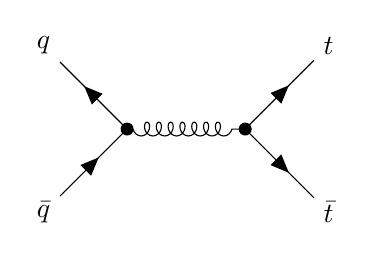
\begin{tikzpicture}[baseline=-0.09cm]
			\begin{feynman}
				\vertex[dot] (a) {};
				\vertex[dot,right= of a] (b) {};
				\vertex[above left= of a] (c) {$q$};
				\vertex[below left= of a] (d) {$\bar{q}$};
				\vertex[above right= of b] (e) {$t$};
				\vertex[below right= of b] (f) {$\bar{t}$};
				
				\diagram* {
					(a) -- [fermion] (c),
					(d) -- [fermion] (a),
					(a) -- [gluon] (b),
					(b) -- [fermion] (e),
					(b) -- [fermion] (f)
					
					%(f) -- [fermion, edge label = $k$] (b),
					%(b) -- [fermion, edge label = $k'$] (e)
				};          
			\end{feynman}        
		\end{tikzpicture}\right\vert^2 \propto g_s^4 
	\end{equation}
	\item $gg\to t\bar{t}$
	\begin{equation}
	\abs{\mathcal{M}_{SM}^{gg}}^2 = \left\vert
	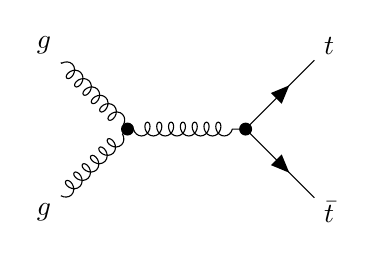
\begin{tikzpicture}[baseline=-0.09cm]
		\begin{feynman}
			\vertex[dot] (a) {};
			\vertex[dot,right= of a] (b) {};
			\vertex[above left= of a] (c) {$g$};
			\vertex[below left= of a] (d) {$g$};
			\vertex[above right= of b] (e) {$t$};
			\vertex[below right= of b] (f) {$\bar{t}$};
			
			\diagram* {
				(a) -- [gluon] (c),
				(d) -- [gluon] (a),
				(a) -- [gluon] (b),
				(b) -- [fermion] (e),
				(b) -- [fermion] (f)
				
				%(f) -- [fermion, edge label = $k$] (b),
				%(b) -- [fermion, edge label = $k'$] (e)
			};          
		\end{feynman}        
	\end{tikzpicture}\right\vert^2 \propto g_s^4 
	\end{equation}
\end{itemize}
Since these SM contributions are common to both the UV and EFT computations, our analysis focuses on the interference terms, where new physics effects appear.

Diagrammatically, the interference terms arise from the overlap between the SM Born-level diagrams shown above and the BSM one-loop diagrams displayed in the left column of Fig.~\ref{fig:diagramstable}, or their EFT counterparts shown in the right column. Each interference term contributes at a specific order in the coupling expansion, scaling either as $g_s^6$ or $g_s^4 y_{DM}^2$, depending on the structure of the BSM loop:

\begin{itemize}
	\item The interference between the SM Born diagram and the first row of Fig.~\ref{fig:diagramstable} contributes at order $g_s^6$. These one-loop diagrams involve only QCD vertices, such as quark-gluon ($q$-$\bar{q}$-$g$) and heavy partner-gluon ($T$-$\bar{T}$-$g$) interactions.
	\item The interference with the second row contributes at order $g_s^4 y_{DM}^2$, as each diagram contains two insertions of the new-physics vertex $t_R$–$T$–$s$, each proportional to $y_{DM}$, in addition to the QCD-like ones.
\end{itemize}

The EFT diagrams carry the same coupling structure as their UV one-loop counterparts. As a result, in the energy regime where the EFT is valid, the total cross section, when expanded in powers of $g_s$ and $y_{DM}$, must match term by term between the two approaches. This insight forms the basis of our strategy for evaluating the EFT's accuracy: we compare the interference contributions to the total cross section, grouping them according to their dependence on the coupling constants.

To carry out these computations, we used the Fixed Order mode of \texttt{MadGraph5\_aMC@NLO} for the next-to-leading-order (NLO) calculations of the UV one-loop model, targeting a precision of 0.1. For the EFT, the evaluations were performed at leading order (LO), also using \texttt{MadGraph\_aMC@NLO}footnote{For the NLO computations, we generated 1,000 Monte Carlo events per mass configuration; for the EFT, we used 10,000 events per point.}. We focused on the interference contributions to the total cross section for the subprocesses $qq \to t\bar{t}$ and $gg \to t\bar{t}$, isolating the terms proportional to $g_s^4 y_{DM}^2$. The parameter scan ranged from $(M_T, M_s) = (200, 190)\, \text{GeV}$ to $(10.0, 9.5)\, \text{TeV}$, thus covering both the validity regime of the EFT and regions where it is expected to break down. In all configurations, we fixed the BSM mass ratio at $M_s / M_T = 0.95$.

The total cross section values proportional to $g_s^4 y_{DM}^2$ obtained from the UV one-loop computations are shown in the upper panels of Fig.~\ref{fig:cs_qq2ttbar_gs4_ydm2}. The lower panels display the ratio $\sigma_{\text{EFT}} / \sigma_{\text{UV}}$, which quantifies the agreement between the EFT prediction and the full UV result. From the plots, we observe a precise agreement between the two approaches up to approximately $M_T \sim 4,\text{TeV}$, consistent with the expected domain of validity of the EFT expansion. However, an exception is noted at the highest mass point, $M_T = 10\, \text{TeV}$ and $M_s=9.5\, \text{TeV}$ for the $gg\to t\bar{t}$ channel, where the EFT result overestimates the UV one-loop calculation by approximately 15\%. We attribute this discrepancy to effects of large logarithms in the UV one-loop computations when BSM masses are significantly greater than the matching scale $\mu$, which in our NLO computations is the mass of the SM $Z$ boson\footnote{Changing the matching scale is not trivial in \texttt{MadGraph5\_aMC@NLO}, and we are currently investigating methods to address this.}.

In the intermediate regime, between $M_T \sim 4,\text{TeV}$ and $M_T \sim 1,\text{TeV}$, the deviation remains moderate, around 10\%. Below $M_T \sim 800,\text{GeV}$, however, the discrepancy becomes more significant. At $M_T = 600,\text{GeV}$, the EFT underestimates the UV result by approximately 20\% for the $gg \to t\bar{t}$ channel and 15\% for $q\bar{q} \to t\bar{t}$.

These results indicate that the $gg \to t\bar{t}$ subprocess is slightly more sensitive to the breakdown of the EFT description as the mass scale decreases, compared to $q\bar{q} \to t\bar{t}$. This sensitivity becomes particularly evident for $M_T \lesssim 1,\text{TeV}$, where the EFT approximation starts to lose accuracy more rapidly.

An interesting detail is observed in the lower panel of the $qq\to t\bar{t}$ plot (Fig.~\ref{fig:cs_qq2ttbar_gs4_ydm2}) at $M_T = 1\, \text{TeV}$ and $M_T = 200\, \text{GeV}$. At these specific points, the ratio of the EFT to UV total cross sections deviates from the general behavior observed in the rest of the parameter scan. We are currently investigating the physical reasons behind this anomalous behavior.

\begin{figure}[h!]
	\centering
	\includegraphics[width=0.48\linewidth]{qq2ttbar_CS.png}
	\includegraphics[width=0.48\linewidth]{gg2ttbar_CS.png}
	\caption{Graphs showing the interference contribution to the total cross section, proportional to $\alpha_s^2 y_{DM}^2$. The upper panels display the values obtained from the UV one-loop calculation, while the lower panels show the ratio $\sigma_{\text{EFT}} / \sigma_{\text{UV}}$. The left plot corresponds to the $q\bar{q} \to t\bar{t}$ channel, and the right plot to $gg \to t\bar{t}$. In both cases, the BSM mass ratio was fixed at $M_s / M_T = 0.95$.}
	\label{fig:cs_qq2ttbar_gs4_ydm2}
\end{figure}


				
				
\chapter{Conclusion and future perspectives}

The Standard Model, despite its remarkable success in describing fundamental particles and their interactions, is acknowledged to be an incomplete theory, with compelling evidence pointing towards the existence of physics Beyond the Standard Model (BSM). Phenomena such as Dark Matter, neutrino masses, and the baryon asymmetry of the universe necessitate new degrees of freedom not accounted for by the SM. While the LHC extensively probes new physics through direct searches, the accumulation of experimental data has continually pushed the mass limits on BSM particles to higher scales, thereby highlighting the growing importance of indirect search methods. In this context, Effective Field Theories (EFTs) provide a useful and systematic framework to describe the low-energy effects of heavy new physics, providing a simplified yet accurate approach to compute theoretical predictions for observables relevant to indirect searches.

In this work, we carried out a theoretical investigation of a systematic method known as the Covariant Derivative Expansion (CDE) for integrating out heavy bosonic and fermionic fields from ultraviolet (UV) models, yielding the corresponding EFT Lagrangian. We illustrated the method through two toy model applications, which allowed us to explore technical aspects that are often omitted or underemphasized in the literature.

The second part of the work focused on testing the accuracy and limitations of the EFT description by comparing its predictions with those of the full one-loop calculation in a concrete, UV-complete BSM model. The model includes a color-triplet vector-like top partner ($\psi_T$) and a real scalar singlet ($s$), the latter acting as a dark matter candidate. Assuming the BSM particles are significantly heavier than the energies probed, we employed Matchete to derive the relevant dimension-six EFT operators contributing to $t\bar{t}$ production at the LHC. The resulting Wilson coefficients were found to be loop-suppressed, with typical magnitudes ranging from $\mathcal{O}(10^{-6})$ to $\mathcal{O}(10^{-4}), \text{TeV}^{-2}$ for $y_{\text{DM}} = 1.0$, and up to $\mathcal{O}(10^{-3}), \text{TeV}^{-2}$ for $y_{\text{DM}} = 5.0$. These values lie well below the current experimental sensitivity, as expected in a weakly coupled scenario.

We then used Monte Carlo simulations to compute the total cross section for $pp \to t\bar{t}$ at leading order, spiting it in $q\bar{q}$ and $gg$ channels, for both the full UV model and its EFT limit. Particularly, we focused on the interference terms proportional to $g_s^4 y_{DM}^2$. Analyzing the results we notice that the EFT reproduced the full model results with high accuracy for heavy masses $M_T \gtrsim 4, \text{TeV}$. In the intermediate regime $1, \text{TeV} \lesssim M_T \lesssim 4, \text{TeV}$, the EFT maintained a deviation of around 10\%. However, for lighter masses $M_T \sim 800, \text{GeV}$, the deviation increased significantly, with the EFT underestimating the full result by 15–20\% or more. This breakdown became more pronounced for $M_T < 800, \text{GeV}$, where the discrepancy rapidly grows. Among the subprocesses, $gg \to t\bar{t}$ exhibited a slightly greater sensitivity to the breakdown of the EFT approximation compared to $q\bar{q} \to t\bar{t}$ as the BSM scale decreased.

For future work, we aim to refine the analysis presented in Chapter~2 and extend it to include the interference contributions to the total cross section that are proportional to $g_s^6$. In addition, we plan to explore the impact of this simple dark matter model on key Standard Model observables, such as the invariant mass distribution of the $t\bar{t}$ pair, the transverse momentum ($p_T$) distribution of the top quark, and the distribution of the transverse angle between the top and antitop quarks. These differential distributions will also serve to complement our EFT analysis, both within and beyond the regime of validity of the effective expansion.







				
				
				
				
				
				
				
				
				
				
				
				
				
				
				
				
				
				
				
				
				
				
				
				
				
				
				
				
				
				
				
				
				
				
				
				
				
				
				
				
				
				
				
				
				
				
				
				
				
				
				
				
				
				
				
				
				
				
				
				
				\newpage
				
				
				
				
				
				
				
				
				
				
				
				
				
				
				
				
				
				
				
				
				
				
				
				
				
				
				
				
				
				
				
				
				
				
				
				
				
				
				
				
				
				
				
				
				
				
				
				
				
				
				
				
				
				
				
				
				
				
				
				
				
				
				
				
				
				
				
				
				
				
				
				
				
				
				
				
				
				
				
				
				
				
				
				
				
				
				
				
				
				
				
				
				
				
				
				
				
				
				
				
				
				
				
				
				
				
				
				
				
				
				
				
				
				
				
				
				
				
				
				
				
				
				
				
				
				
				
				
				
				
				
				
				
				
				
				
				
				
				
				
				
				
				
				
				
				
				
				
				
				
				
				
				
				
				
				
				
				
				
				
				
				
				
				
				
				
				
				
				
				
				
				
				
				
				
				
				
				
				
				
				
				
				
				
				
				\newpage
				\appendix
				
				\chapter{Calculations of the toy model EFT}
				
				
				\section{Solving the classical equation of motion for the heavy fields}\label{ap:solEOM}
				
				In chapter \ref{ch:CDE}, we found the following equations of motion for the heavy fields of the toy model:
				\begin{align}
					&\left[\square + M_s^2+\frac{1}{2}y_{Hs} h^2 + \frac{\lambda_s}{6}s_c^2 \right]s_c = - y_{DM}\left( \bar{\psi}_T t_R + \bar{t}_R \psi_T \right)\label{eq:s_c1}\\
					&\left(i\slashed{D}^{\psi_{T}} - M_T\right)\psi_{T,c} = y_{DM} t_R s_c\\
					&\left(i\slashed{D}^{\psi_{T}} + M_T\right)\bar{\psi}_{T,c} = -y_{DM}\bar{t}_R s_c
				\end{align}
				
				In order to solve them, we start by rewriting the last two equations:
				\begin{align}
					&\psi_{T,c} =  y_{DM} \left(i\slashed{D}^{\psi_{T}} - M_T\right)^{-1}t_R s_c \label{eq:EOM1}\\
					&\bar{\psi}_{T,c} = - y_{DM}\bar{t}_R \left(i\overleftarrow{\slashed{D}}^{\psi_{T}} + M_T\right)^{-1} s_c\label{eq:EOM2}
				\end{align}
				
				Since we are interested in operators up to dimension six, we can expand the expression above up to order $\mathcal{O}(\frac{1}{M_T^2})$:
				\begin{align}
					&\psi_{T,c} =  -\frac{y_{DM}}{M_T} \left(1 + \frac{i\slashed{D}^{\psi_{T}}}{M_T}\right)t_R s_c\\
					&\bar{\psi}_{T,c} = - \frac{y_{DM}}{M_T} \bar{t}_R\left(1 - \frac{i\overleftarrow{\slashed{D}}^{\psi_{T}}}{  M_T}\right) s_c
				\end{align}
				
				Substituting this into Eq. (\ref{eq:s_c1}):
				%\begin{align}
				%	&\left[\square + M_s^2+2y_{Hs} h^2 + \frac{\lambda_s}{6}s_c^2\right]s_c =  y_{DM}^2\left[ \left(\left(i\slashed{D}^{\psi_{T}} + M_T\right)^{-1}\bar{t}_R s_c\right) t_R - \bar{t}_R  \left(i\slashed{D}^{\psi_{T}} - M_T\right)^{-1}\bar{t}_R s_c\right]\nonumber\\
				%	&\left[\square + M_s^2+2y_{Hs} h^2 + \frac{\lambda_s}{6}s_c^2 + y_{DM}^2\left(i\slashed{D}^{\psi_{T}} - M_T\right)^{-1}\bar{t}_R - y_{DM}^2 t_R\left(i\slashed{D}^{\psi_{T}} + M_T\right)^{-1}\bar{t}_R \right]s_c = 0\nonumber\\
				% &\hspace{3cm} \implies   s_c = 0 \implies \psi_{T,c} = 0 \ \ \ \text{and} \ \ \ \bar{\psi}_{T,c} = 0
				%\end{align}
				\begin{align}
					&\left[\square + M_s^2+\frac{1}{2}y_{Hs} h^2 + \frac{\lambda_s}{6}s_c^2\right]s_c =  \frac{y_{DM}^2}{M_T}\left[ \bar{t}_R \left(1 - \frac{i\overleftarrow{\slashed{D}}^{\psi_{T}}}{  M_T}\right)s_c t_R + \bar{t}_R  \left(1 + \frac{i\slashed{D}^{\psi_{T}}}{M_T}\right)t_R s_c\right]\nonumber\\
					&\left[\square + M_s^2+\frac{1}{2}y_{Hs} h^2 + \frac{\lambda_s}{6}s_c^2 +i \frac{y_{DM}^2}{M_T^2}\bar{t}_R \overleftarrow{\slashed{D}}^{\psi_{T}} t_R -i \frac{y_{DM}^2}{M_T^2} \bar{t}_R  \slashed{D}^{\psi_{T}}t_R  \right]s_c = 0
					% &\hspace{3cm} \implies   s_c = 0 \implies \psi_{T,c} = 0 \ \ \ \text{and} \ \ \ \bar{\psi}_{T,c} = 0
				\end{align}
				
				To solve this equation order by order, we write the solution $s_c$ as:
				\begin{align}
					s_c = s_c^{(2)} + s_c^{(4)} + s_c^{(6)}
				\end{align}
				
				\noindent where $s_c^{(n)}$ contains operators with mass dimension $n$ multiplied by prefactors that scale as $M^{1-n}$, where $M$ represents a heavy mass scale such as $M_s$ and $M_T$. Grouping terms in the equation of motion by operator dimension, we obtain:
				\begin{align}
					&M_s^2  s_c^{(2)} = 0 \nonumber\\
					&\left[\square +\frac{1}{2} y_{Hs} h^2\right]s_c^{(2)} + M^2 s_c^{(4)} = 0\nonumber\\
					&\left[\square +\frac{1}{2} y_{Hs} h^2\right]s_c^{(4)} + M^2 s_c^{(6)} +\frac{\lambda_s}{6}[s_c^{(2)}]^3 +i \frac{y_{DM}^2}{M_T^2}\bar{t}_R \overleftarrow{\slashed{D}}^{\psi_{T}} t_R s_c^{(2)}-i \frac{y_{DM}^2}{M_T^2} \bar{t}_R  \slashed{D}^{\psi_{T}}t_R s_c^{(2)}= 0
				\end{align}
				
				From the first equation, we immediately see that $s_c^{(2)}=0$. his result eliminates the source term in the second equation, implying $s_c^{(4)} = 0$ as well. With both $s_c^{(2)}$ and $s_c^{(4)} $ all remaining terms in the third equation also vanish, leading to $s_c^{(6)}=0$. Thus, up to and including dimension-6 contributions, the classical solution is simply:
				\begin{align}
					s_c=0
				\end{align} 
				
				Substituting this into Eq. (\ref{eq:EOM1}) and (\ref{eq:EOM2}) implies that:
				\begin{align}
					\psi_{T,c} = 0 \ \ \ \text{and} \ \ \ \bar{\psi}_{T,c} = 0
				\end{align}
				
				Therefore, the classical solution for the heavy fields it is zero.
				
				\section{List of interaction matrices}\label{ap:int_mt}
				
				When generalizing the matching method to include the effects of integrating out fermions, we introduced interaction matrices, as defined in Equations (\ref{eq:int_mt}) and (\ref{eq:int_mt1}). The elements of these matrices take the general form:
				\begin{align}
					\left(X_{AB}\right)_{ij}\equiv -\frac{\delta^2 \mathcal{L}_{UV, \text{int}}}{\delta A_i \delta B_j}\bigg\vert_{A=A_b,B = B_b}
				\end{align}
				Here, $A$ and $B$epresent arbitrary scalar or fermionic fields, and $\mathcal{L}_{UV, \text{int}}$ denotes the interaction part of the UV Lagrangian. The indices $i$ and $j$ collectively account for all indices carried by the fields $A$ and $B$.
				
				For our specific toy model, the interaction Lagrangian is given by:
				\begin{align}
					\mathcal{L}_{UV,\, \text{int}} =  y_{DM} \left( \bar{\psi}_T t_R + \bar{t}_R \psi_T \right) s  - y_{Ht}h\left(\bar{t}_L t_R + \bar{t}_R t_L\right)-\frac{1}{4}y_{Hs} h^2 s^2 - \frac{\lambda_s}{4!}s^4  - \frac{\lambda_h}{4!} h^4
				\end{align}
				
				Following these definitions, we can now derive the specific forms of the interaction matrices for our model:
				\begin{align}
					&\tilde{\mathbf{X}}_{\Psi\Psi} =\begin{pmatrix}
						X_{\psi_T\psi_T} & X_{\psi_T \bar{\psi}_T}\ccj^{-1} &0\\
						\ccj X_{\bar{\psi}_T \psi_T} &\ccj X_{\bar{\psi}_T \bar{\psi}_T}\ccj^{-1} &0\\
						0 &0 &0
					\end{pmatrix} =0_{3\times3}\\
					&\tilde{\mathbf{X}}_{\Psi\psi}  = \begin{pmatrix}
						X_{\psi_T\psi_T} & X_{\psi_T \bar{t}}\ccj^{-1} &0\\
						\ccj X_{\bar{\psi}_T t} &\ccj X_{\bar{\psi}_T \bar{t}}\ccj^{-1}&0\\
						0 &0 &0
					\end{pmatrix} = y_{DM} s_c 
					\begin{pmatrix} 
						0 &P_L\ccj^{-1} &0 \\
						\ccj P_R &0 &0\\
						0 &0 &0
					\end{pmatrix} = 0_{3\times3}\\
					&\tilde{\mathbf{X}}_{\psi\Psi}  = \begin{pmatrix}
						X_{t \psi_T} & X_{t \bar{\psi}_T}\ccj^{-1} &0\\
						\ccj X_{\bar{t} \psi_T} &\ccj X_{\bar{t} \bar{\psi}_T}\ccj^{-1} &0\\
						0 &0 &0
					\end{pmatrix} = y_{DM} s_c 
					\begin{pmatrix} 
						0 &P_L \ccj^{-1} &0\\
						\ccj P_R &0 &0\\
						0 &0 &0
					\end{pmatrix} = 0_{3\times3}%\frac{y_{DM}^2}{m_S^2}\left( \bar{\psi}_T t_R + \bar{t}_R \psi_T \right)  
					%\begin{pmatrix} 
					%P_R &0 \\
					%0 &P_L
					%\end{pmatrix} 
					\\
					&\tilde{\mathbf{X}}_{\Psi\phi} = \begin{pmatrix}
						0&0 &X_{\psi_T h}\\ 
						0&0&\ccj X_{\bar{\psi}^T h}\\
						0&0 &0
					\end{pmatrix} =  0_{3\times3}\\
					&\tilde{\mathbf{X}}_{\phi\Psi} =\begin{pmatrix}
						0 &0 &0\\
						0&0&0\\
						X_{ h\psi_T} & X_{h\bar{\psi}^T }\ccj^{-1} &0
					\end{pmatrix}  = 0_{3\times3}\\
					&\tilde{\mathbf{X}}_{\Psi\Phi} =  \begin{pmatrix}
						0&0&X_{\psi_T s} \\0&0&\ccj X_{\bar{\psi}_T s} \\0&0&0
					\end{pmatrix}= y_{DM}\begin{pmatrix}
						0&0&\bar{t}_R\\ 0&0&\ccj t_R\\ 0&0&0
					\end{pmatrix}\\
					&\tilde{\mathbf{X}}_{\Phi\Psi} =\begin{pmatrix}
						0&0&0 \\0&0&0\\ X_{s \psi_T } & X_{s\bar{\psi}_T }\ccj^{-1}&0 
					\end{pmatrix} =  y_{DM}\begin{pmatrix}
						0&0&0\\0&0&0\\
						\bar{t}_R & t_R\ccj^{-1} &0
					\end{pmatrix}\\
					&\tilde{\mathbf{X}}_{\psi\psi}  = \begin{pmatrix}
						X_{t t} & X_{t \bar{t}}\ccj^{-1} &0\\
						\ccj X_{\bar{t} t} &\ccj X_{\bar{t} \bar{t}}\ccj^{-1} &0\\
						0&0&0
					\end{pmatrix} = y_{Ht} \begin{pmatrix}
						0 &h \ccj^{-1} &0\\
						\ccj h & 0 &0\\
						0&0&0
					\end{pmatrix} \\
					&\tilde{\mathbf{X}}_{\psi\Phi} = \begin{pmatrix}
						0& 0 &X_{t s} \\ 0&0&\ccj X_{\bar{t} s}\\ 0&0&0
					\end{pmatrix} = y_{DM} \begin{pmatrix}
						0&0 &\bar{\psi}_{T,c} P_R \\ 0&0& \ccj P_L\psi_{T,c} \\0&0&0
					\end{pmatrix} =   0_{3\times3}\\
					& \tilde{\mathbf{X}}_{\Phi\psi} = \begin{pmatrix}
						0&0&0\\ 0&0&0\\ X_{s t} &X_{s\bar{t}}\ccj^{-1} &0
					\end{pmatrix} = y_{DM}\begin{pmatrix}
						0&0&0\\ 0&0&0\\
						\bar{\psi}_{T,c}P_R &P_L\psi_{T,c}\ccj^{-1} &0
					\end{pmatrix} =  0_{3\times3}\\
					&\tilde{\mathbf{X}}_{\psi\phi} = \begin{pmatrix}
						0&0 &X_{t h}\\ 0&0& \ccj X_{\bar{t} h} \\ 0&0&0
					\end{pmatrix} = y_{Ht}\begin{pmatrix}
						0&0& \bar{t} \\ 0&0& \ccj t \\ 0&0&0
					\end{pmatrix}\\
					&\tilde{\mathbf{X}}_{\phi\psi}  = \begin{pmatrix}
						0&0&0\\ 0&0&0\\ X_{h t} &X_{h \bar{t}}\ccj^{-1} &0
					\end{pmatrix} = y_{Ht}\begin{pmatrix}
						\bar{t} & t\ccj^{-1}
					\end{pmatrix}\\
					&\tilde{\mathbf{X}}_{\Phi\phi} = \begin{pmatrix}
						0 &0 &0\\ 0&0&0 \\ 0&0 &X_{sh}
					\end{pmatrix} = y_{Hs}h s_c = \begin{pmatrix}
						0 &0 &0\\ 0&0&0 \\ 0&0 &1
					\end{pmatrix}= 0_{3\times 3}\\
					&\tilde{\mathbf{X}}_{\Phi\Phi} = \begin{pmatrix}
						0 &0 &0\\ 0&0&0 \\ 0&0 &X_{ss}
					\end{pmatrix}  = \left(\frac{1}{2} y_{Hs} h^2 + \frac{\lambda_s}{2}s_c^2\right)\begin{pmatrix}
						0 &0 &0\\ 0&0&0 \\ 0&0 &1
					\end{pmatrix} = \frac{1}{2} y_{Hs} h^2 \begin{pmatrix}
						0 &0 &0\\ 0&0&0 \\ 0&0 &1
					\end{pmatrix}\\
					&\tilde{\mathbf{X}}_{\phi\phi} = \begin{pmatrix}
						0 &0 &0\\ 0&0&0 \\ 0&0 &X_{hh}
					\end{pmatrix} = \left(\frac{1}{2} y_{Hs} s_c^2 + \frac{\lambda_h}{2}h^2\right)\begin{pmatrix}
						0 &0 &0\\ 0&0&0 \\ 0&0 &1
					\end{pmatrix} = \frac{\lambda_h}{2}h^2\begin{pmatrix}
						0 &0 &0\\ 0&0&0 \\ 0&0 &1
					\end{pmatrix}
				\end{align}
				
				After computing this matrices, we must use these results to calculate the following shifts:
				\begin{align}
					&\bar{\Delta}_A \equiv \Delta_{A} - \tilde{\mathbf{X}}_{A\psi}\Delta_\psi^{-1}\tilde{\mathbf{X}}_{\psi A}\\
					&\bar{\mathbf{X}}_{AB} = \tilde{\mathbf{X}}_{AB} - \tilde{\mathbf{X}}_{A\psi}\Delta^{-1}_\psi\tilde{\mathbf{X}}_{\psi B}
				\end{align} 
				
				As a result, we obtain:
				\begin{align}
					&\bar{\mathbf{X}}_{\Psi\Psi} = \tilde{\mathbf{X}}_{\Psi\Psi} - \tilde{\mathbf{X}}_{\Psi\psi}\Delta^{-1}_\psi\tilde{\mathbf{X}}_{\psi \Psi}  = 0_{3\times 3}\\
					&\bar{\mathbf{X}}_{\Psi\psi}  = \tilde{\mathbf{X}}_{\Psi\psi} - \tilde{\mathbf{X}}_{\Psi\psi}\Delta^{-1}_\psi\tilde{\mathbf{X}}_{\psi \psi} = 0_{3\times 3}\\
					&\bar{\mathbf{X}}_{\psi\Psi}  = \tilde{\mathbf{X}}_{\psi\Psi} - \tilde{\mathbf{X}}_{\psi\psi}\Delta^{-1}_\psi\tilde{\mathbf{X}}_{\psi \Psi} = 0_{3\times 3}
					\\
					&\bar{\mathbf{X}}_{\Psi\phi} = \tilde{\mathbf{X}}_{\Psi\phi} - \tilde{\mathbf{X}}_{\Psi\psi}\Delta^{-1}_\psi\tilde{\mathbf{X}}_{\psi \phi} = 0_{3\times 3}\label{eq:X_Psiphi}\\
					&\bar{\mathbf{X}}_{\phi\Psi} =\tilde{\mathbf{X}}_{\phi\Psi} - \tilde{\mathbf{X}}_{\phi\psi}\Delta^{-1}_\psi\tilde{\mathbf{X}}_{\psi \Psi} = 0_{3\times 3}\label{eq:X_phiPsi}\\
					&\bar{\mathbf{X}}_{\Psi\Phi} =\tilde{\mathbf{X}}_{\Psi\Phi} - \tilde{\mathbf{X}}_{\Psi\psi}\Delta^{-1}_\psi\tilde{\mathbf{X}}_{\psi \Phi} = \tilde{\mathbf{X}}_{\Psi\Phi} \\
					&\bar{\mathbf{X}}_{\Phi\Psi} =\tilde{\mathbf{X}}_{\Phi\Psi} - \tilde{\mathbf{X}}_{\Phi\psi}\Delta^{-1}_\psi\tilde{\mathbf{X}}_{\psi \Psi} = \tilde{\mathbf{X}}_{\Phi\Psi} \\
					&\bar{\mathbf{X}}_{\psi\psi}  = \tilde{\mathbf{X}}_{\psi\psi} - \tilde{\mathbf{X}}_{\psi\psi}\Delta^{-1}_\psi\tilde{\mathbf{X}}_{\psi \psi}  \\
					&\bar{\mathbf{X}}_{\psi\Phi} = \tilde{\mathbf{X}}_{\psi\Phi} - \tilde{\mathbf{X}}_{\psi\psi}\Delta^{-1}_\psi\tilde{\mathbf{X}}_{\psi \Phi} = 0_{3\times 3}\\
					& \bar{\mathbf{X}}_{\Phi\psi} = \tilde{\mathbf{X}}_{\Phi\psi} - \tilde{\mathbf{X}}_{\Phi\psi}\Delta^{-1}_\psi\tilde{\mathbf{X}}_{\psi \psi} = 0_{3\times 3}\\
					&\bar{\mathbf{X}}_{\phi\psi}  = \tilde{\mathbf{X}}_{\phi\psi} - \tilde{\mathbf{X}}_{\phi\psi}\Delta^{-1}_\psi\tilde{\mathbf{X}}_{\psi \psi} \\
					&\bar{\mathbf{X}}_{\Phi\phi} = \tilde{\mathbf{X}}_{\Phi\phi} - \tilde{\mathbf{X}}_{\Phi\psi}\Delta^{-1}_\psi\tilde{\mathbf{X}}_{\psi \phi} = 0_{3\times 3}\\
					&\bar{\mathbf{X}}_{\Phi\Phi} = \tilde{\mathbf{X}}_{\Phi\Phi} - \tilde{\mathbf{X}}_{\Phi\psi}\Delta^{-1}_\psi\tilde{\mathbf{X}}_{\psi \Phi} = \tilde{X}_{\Phi\Phi}\\
					&\bar{\mathbf{X}}_{\phi\phi} = \tilde{\mathbf{X}}_{\phi\phi} - \tilde{\mathbf{X}}_{\phi\psi}\Delta^{-1}_\psi\tilde{\mathbf{X}}_{\psi \phi} \nonumber\\
					&\bar{\Delta}_\Psi = \Delta_{\Psi} - \tilde{\mathbf{X}}_{\Psi\psi}\Delta_\psi^{-1}\tilde{\mathbf{X}}_{\psi \Psi} = \Delta_{\Psi}\\
					&\bar{\Delta}_\psi = \Delta_{\psi} - \tilde{\mathbf{X}}_{\psi\psi}\Delta_\psi^{-1}\tilde{\mathbf{X}}_{\psi \psi} \\
					&\bar{\Delta}_\Phi = \Delta_{\Phi} - \tilde{\mathbf{X}}_{\Phi\psi}\Delta_\psi^{-1}\tilde{\mathbf{X}}_{\psi \Phi} = \Delta_{\Phi}\\
					&´\bar{\Delta}_\phi = \Delta_{\phi} - \tilde{\mathbf{X}}_{\phi\psi}\Delta_\psi^{-1}\tilde{\mathbf{X}}_{\psi \phi} 
				\end{align}
				
				\section{Scalar path integral contribution}
				
				As we saw in the calculation of the toy model one-loop EFT Lagrangian, the scalar path integral contribution is given by (Eq.~\ref{eq:exp2}):
				\begin{align}
					\mathcal{L}^{\text{1-loop}}_{EFT,SF} &= -\frac{i}{2}\sum_{n=1}^{\infty} \frac{1}{n}\int \frac{d^dq}{(2\pi)^d}  \tr\Bigg[\frac{2q\cdot P_\Phi - P_\Phi^2 +\frac{1}{2} y_{Hs} h^2}{q^2 - M_\Phi^2}\nonumber\\
					&\hspace{2.cm}- \frac{y_{DM}^2}{q^2 - M_\Phi^2} \sum^{+\infty}_{l=3} \begin{pmatrix}
						\bar{t}_R & t_R^T\ccj^{-1} 
					\end{pmatrix}  \frac{ \left[(-\slashed{q}+M_T)(-\slashed{P}_{\Psi} )\right]^l(-\slashed{q}+ M_T)}{(q^2-M_T^2)^{l+1}}\begin{pmatrix}
						t_R\\ \ccj^{-1}\bar{t}_R^T
					\end{pmatrix}\Bigg]^n\bigg\vert_{\text{hard}}\label{eq:Aexp2}
				\end{align}
				By computing the first values of $n$ in the expression above we will all operators up to dimension six. In order to keep the calculation as clear as possible, we will compute the contribution of each value of $n$ separately and then summing all at the end. Starting with $n=1$ contribution.
				
				
				\subsection{Computing the $n=1$ contribution coming from the scalar path integral }\label{ap:n_1_SF}
				
				Setting $n=1$ into Eq.~(\ref{eq:exp2}) give us:
				\begin{align}
					&\mathcal{L}^{\text{1-loop}}_{EFT,SF}[\phi_b,\psi_b] \supset\nonumber\\
					-&\frac{i}{2}\int \frac{d^dq}{(2\pi)^d}  \tr\Bigg[\frac{\frac{1}{2} y_{Hs} h^2}{q^2 - M_\Phi^2}
					- \frac{y_{DM}^2}{q^2 - M_\Phi^2} \sum^{+\infty}_{l=3} \begin{pmatrix}
						\bar{t}_R & t_R^T\ccj^{-1} 
					\end{pmatrix}  \frac{ \left[(-\slashed{q}+M_T)(-\slashed{P}_{\Psi} )\right]^l(-\slashed{q}+ M_T)}{(q^2-M_T^2)^{l+1}}\begin{pmatrix}
						t_R\\ \ccj^{-1}\bar{t}_R^T
					\end{pmatrix}\Bigg]\bigg\vert_{\text{hard}} \label{eq:An=1}
				\end{align}
				\noindent where the $P_\Phi$ are ordinary derivatives and, as a consequence, these terms does not contributes since they act on the identity on the right. Furthermore, we can see that all terms will give us operators up to dimension six.
				
				To proceed we need to compute the contributions coming from the $l$ summation in the expression above. Beginning with $l=0$, we have:
				
				\begin{align}
					\begin{pmatrix}
						\bar{t}_R & t_R^T\ccj^{-1} 
					\end{pmatrix}  \frac{ (-\slashed{q}+ M_T)}{(q^2-M_T^2)}\begin{pmatrix}
						t_R\\ \ccj^{-1}\bar{t}_R^T
					\end{pmatrix} = \bar{t}_R \frac{(-\slashed{q} + M_T)}{(q^2 - M_T^2)}t_R + t^T_R \ccj^{-1}\frac{(-\slashed{q} + M_T)}{(q^2 - M_T^2)}\ccj^{-1}\bar{t}^T_R
				\end{align}
				
				Since we have right-hand projectors in the fields, only the terms with an odd number of gamma matrices between the fields will not vanish. To see why, consider a generic term with $m$ gamma matrices:
				\begin{align}
					\bar{t}_R \underbrace{\gamma^\mu...\gamma^\nu}_{m \ \text{times}} t_R = (P_R t)^\dagger \gamma^0 \gamma^\mu...\gamma^\nu P_R t = t^\dagger P_R \gamma^0 \gamma^\mu...\gamma^\nu P_R t 
				\end{align}
				
				Using that $P_{R, L} \gamma^\mu = \gamma^\mu P_{L,R} $:
				\begin{align}
					\bar{t}_R \gamma^\mu...\gamma^\nu t_R = \bar{t} P_L \gamma^\mu...\gamma^\nu P_R t &= 
					\begin{cases}
						\bar{t}  \gamma^\mu...\gamma^\nu P_R^2 t, \, \text{for odd $m$}\\
						\bar{t}\gamma^\mu...\gamma^\nu P_L P_R t, \, \text{for an even $m$}
					\end{cases}\nonumber\\
					& = \begin{cases}
						\bar{t}  \gamma^\mu...\gamma^\nu P_R t, \, \text{for odd $m$}\\
						0, \, \text{for even $m$}
					\end{cases}
				\end{align}
				
				Therefore, the non vanishing contributions in $l=0$ are:
				\begin{align}
					\begin{pmatrix}
						\bar{t}_R & t_R^T\ccj^{-1} 
					\end{pmatrix}  \frac{ (-\slashed{q}+ M_T)}{(q^2-M_T^2)}\begin{pmatrix}
						t_R\\ \ccj^{-1}\bar{t}_R^T
					\end{pmatrix} =-\bar{t}_R \frac{\slashed{q}}{(q^2 - M_T^2)}t_R  - t^T_R\ccj^{-1}\frac{\slashed{q}}{(q^2 - M_T^2)}\ccj^{-1}\bar{t}^T_R
				\end{align}
				
				Using that $\ccj^{-1} = -\ccj$, $\ccj \gamma^\mu \ccj^{-1} = -(\gamma^\mu)^T$ and when contracting spinor indices we have $\psi^T \Gamma^T \bar{\psi}^T = - \bar{\psi}\Gamma\psi$:
				\begin{align}
					\begin{pmatrix}
						\bar{t}_R & t_R^T\ccj^{-1} 
					\end{pmatrix}  \frac{ (-\slashed{q}+ M_T)}{(q^2-M_T^2)}\begin{pmatrix}
						t_R\\ \ccj^{-1}\bar{t}_R^T
					\end{pmatrix} &=-\bar{t}_R \frac{\slashed{q}}{(q^2 - M_T^2)}t_R  - t^T_R \frac{(\gamma^\mu)^Tq_\mu}{(q^2 - M_T^2)}\bar{t}^T_R\nonumber\\
					&=-\bar{t}_R \frac{\slashed{q}}{(q^2 - M_T^2)}t_R  + \bar{t}_R \frac{\slashed{q}}{(q^2 - M_T^2)}t_R\nonumber\\
					&=0\label{eq:Al=0}
				\end{align}
				
				This result show us that there is no contribution for $l=0$.
				
				For $l=1$, the contribution is: 
				\begin{align}
					l=1 \implies \begin{pmatrix}
						\bar{t}_R & t_R^T\ccj^{-1} 
					\end{pmatrix}  \frac{ (-\slashed{q}+M_T)(-\slashed{P}_{\Psi} )(-\slashed{q}+ M_T)}{(q^2-M_T^2)^{2}}\begin{pmatrix}
						t_R\\ \ccj^{-1}\bar{t}_R^T
					\end{pmatrix}
				\end{align}
				
				Since terms with an even number of gamma matrices vanishes, the non-null contributions for the numerator of the expression above are:
				\begin{align}
					(-\slashed{q}+M_T)(-\slashed{P}_{\Psi} )(-\slashed{q}+ M_T) = -\slashed{q}\slashed{P}_{\Psi}\slashed{q} - M_T^2\slashed{P}_{\Psi}
				\end{align}
				
				Using the anticommutation relation of the gamma matrices:
				\begin{align}
					(-\slashed{q}+M_T)(-\slashed{P}_{\Psi} )(-\slashed{q}+ M_T) &= -2q\cdot  P_{\Psi}\slashed{q}+\slashed{P}_{\Psi}\slashed{q}\slashed{q} - M_T^2\slashed{P}_{\Psi}\nonumber\\
					&= -2q\cdot  P_{\Psi}\slashed{q}+\slashed{P}_{\Psi}q^2 - M_T^2\slashed{P}_{\Psi}
				\end{align}
				
				In the $n=1$ contribution for the effective Lagrangian, the loop momenta appears only in the $l$ summation. Therefore, we can anticipate some steps that are done when using dimensional regularization to compute the loop integral. Due to symmetry, we substitute $q^\mu q^\nu \to \frac{g^{\mu\nu}}{d} q^2$ when computing the loop integral. Then, if we already do this:
				\begin{align}
					(-\slashed{q}+M_T)(-\slashed{P}_{\Psi} )(-\slashed{q}+ M_T) 
					&= -\frac{2}{d}  \slashed{P}_{\Psi}q^2+\slashed{P}_{\Psi}q^2 - M_T^2\slashed{P}_{\Psi}
				\end{align}
				
				Rewriting $d$ as $4-\epsilon$ and expanding up to order $\mathcal{O}(\epsilon)$:
				\begin{align}
					(-\slashed{q}+M_T)(-\slashed{P}_{\Psi} )(-\slashed{q}+ M_T) 
					&=\left(-\frac{1}{2} + \frac{\epsilon}{8}\right)  \slashed{P}_{\Psi}q^2+\slashed{P}_{\Psi}q^2- M_T^2\slashed{P}_{\Psi}\nonumber\\
					& = \left(\frac{1}{2} + \frac{\epsilon}{8}\right) \slashed{P}_{\Psi}q^2- M_T^2\slashed{P}_{\Psi}
				\end{align}
				
				Substituting this in the $l=1$ contribution for the summation and using:
				\begin{align}
					\slashed{P}_{\Psi} = \begin{pmatrix}
						\slashed{P}_{\psi_T} &0\\ 0 &\slashed{P}_{\psi_T}^\ccj
					\end{pmatrix}
				\end{align}
				we get:
				\begin{align}
					\begin{pmatrix}
						\bar{t}_R & t_R^T\ccj^{-1} 
					\end{pmatrix}  \frac{ (-\slashed{q}+M_T)(-\slashed{P}_{\psi_T} )(-\slashed{q}+ M_T)}{(q^2-M_T^2)^{2}}\begin{pmatrix}
						t_R\\ \ccj^{-1}\bar{t}_R^T
					\end{pmatrix} = \frac{\left(\left(\frac{1}{2} + \frac{\epsilon}{8}\right) q^2- M_T^2\right)}{(q^2 - M_T^2)^2}\left[\bar{t}_R\slashed{P}_{\Psi}t_R + t^T_R \ccj^{-1}\slashed{P}_{\psi_T}\ccj^{-1}\bar{t}^T_R \right]
				\end{align}
				
				Rewriting the second term using the same identities of the $l=0$ case:
				\begin{align}
					\begin{pmatrix}
						\bar{t}_R & t_R^T\ccj^{-1} 
					\end{pmatrix}  \frac{ (-\slashed{q}+M_T)(-\slashed{P}_{\Psi} )(-\slashed{q}+ M_T)}{(q^2-M_T^2)^{2}}\begin{pmatrix}
						t_R\\ \ccj^{-1}\bar{t}_R^T
					\end{pmatrix} &= \frac{\left(\left(\frac{1}{2} + \frac{\epsilon}{8}\right) q^2- M_T^2\right)}{(q^2 - M_T^2)^2}\left[\bar{t}_R\slashed{P}_{\psi_T}t_R + t^T_R (\gamma^\mu)^T P_{\psi_T, \mu}\bar{t}^T_R \right]\nonumber\\
					&= \frac{\left(\left(\frac{1}{2} + \frac{\epsilon}{8}\right) q^2- M_T^2\right)}{(q^2 - M_T^2)^2}\left[\bar{t}_R\slashed{P}_{\psi_T}t_R - \bar{t}_R \gamma^\mu P^T_{\psi_T, \mu}t_R \right]
				\end{align}
				
				Here the transpose in the derivative means that it acts on the left. Therefore, to keep this clear we can introduce an arrow to indicate the action of the covariant derivative:
				\begin{align}
					\begin{pmatrix}
						\bar{t}_R & t_R^T\ccj^{-1} 
					\end{pmatrix}  \frac{ (-\slashed{q}+M_T)(-\slashed{P}_{\Psi} )(-\slashed{q}+ M_T)}{(q^2-M_T^2)^{2}}\begin{pmatrix}
						t_R\\ \ccj^{-1}\bar{t}_R^T
					\end{pmatrix} &=\frac{\left(\left(\frac{1}{2} + \frac{\epsilon}{8}\right) q^2- M_T^2\right)}{(q^2 - M_T^2)^2}\left[\bar{t}_R\slashed{P}_{\psi_T}t_R - \bar{t}_R \overleftarrow{\slashed{P}}_{\psi_T}t_R \right]
				\end{align}
				
				Using that $P_\mu = i D_\mu$ and keeping the chirality projectors explicitly:
				\begin{align}
					\begin{pmatrix}
						\bar{t}_R & t_R^T\ccj^{-1} 
					\end{pmatrix}  \frac{ (-\slashed{q}+M_T)(-\slashed{P}_{\Psi} )(-\slashed{q}+ M_T)}{(q^2-M_T^2)^{2}}\begin{pmatrix}
						t_R\\ \ccj^{-1}\bar{t}_R^T
					\end{pmatrix} &=i\frac{\left(\left(\frac{1}{2} + \frac{\epsilon}{8}\right) q^2- M_T^2\right)}{(q^2 - M_T^2)^2}\left[\bar{t}\, \gamma^\mu\, P_R\, D_\mu t - D_\mu \bar{t} \,\gamma^\mu\, P_R \, t \right]\label{eq:Al=1}
				\end{align}
				
				For $l=2$, we have:
				\begin{align}
					l=2 \implies \begin{pmatrix}
						\bar{t}_R & t_R\ccj^{-1} 
					\end{pmatrix}  \frac{ (-\slashed{q}+M_T)(-\slashed{P}_{\Psi} )(-\slashed{q}+M_T)(-\slashed{P}_{\Psi} )(-\slashed{q}+ M_T)}{(q^2-M_T^2)^{3}}\begin{pmatrix}
						t_R\\ \ccj^{-1}\bar{t}_R
					\end{pmatrix} 
				\end{align}
				
				Focusing in the numerator of the fraction above: 
				\begin{align}
					&(-\slashed{q}+M_\Psi)(-\slashed{P}_{\Psi} )(-\slashed{q}+M_\Psi)(-\slashed{P}_{\Psi} )(-\slashed{q}+ M_\Psi) = (\slashed{q}\slashed{P}_{\Psi}-M_\Psi\slashed{P}_{\Psi})(\slashed{q}\slashed{P}_{\Psi}-M_\Psi\slashed{P})(-\slashed{q}+ M_\Psi)\nonumber\\
					&\hspace{4cm} = (\slashed{q}\slashed{P}_{\Psi}\slashed{q}\slashed{P}_{\Psi} - M_\Psi\slashed{q}\slashed{P}_{\Psi}\slashed{P}_{\Psi} - M_\Psi\slashed{P}_{\Psi}\slashed{q}\slashed{P}_{\Psi} + M_\Psi^2\slashed{P}_{\Psi}\slashed{P}_{\Psi})(-\slashed{q}+ M_\Psi)\nonumber\\
					& \hspace{4cm}= -\slashed{q}\slashed{P}_{\Psi}\slashed{q}\slashed{P}_{\Psi}\slashed{q} + M_\Psi\slashed{q}\slashed{P}_{\Psi}\slashed{P}_{\Psi}\slashed{q} + M_\Psi\slashed{P}_{\Psi}\slashed{q}\slashed{P}_{\Psi}\slashed{q} - M_\Psi^2\slashed{P}_{\Psi}\slashed{P}_{\Psi}\slashed{q}\nonumber\\& \hspace{4.4cm} + M_\Psi\slashed{q}\slashed{P}_{\Psi}\slashed{q}\slashed{P}_{\Psi} - M_\Psi^2\slashed{q}\slashed{P}_{\Psi}\slashed{P}_{\Psi} - M_\Psi^2\slashed{P}_{\Psi}\slashed{q}\slashed{P}_{\Psi} + M_\Psi^3\slashed{P}_{\Psi}\slashed{P}_{\Psi}
				\end{align}
				
				Next, we discard terms containing an even number of gamma matrices, as we shown at the $l=0$ term calculation:
				\begin{align}
					&(-\slashed{q}+M_\Psi)(-\slashed{P}_{\Psi} )(-\slashed{q}+M_\Psi)(-\slashed{P}_{\Psi} )(-\slashed{q}+ M_\Psi)=-\slashed{q}\slashed{P}_{\Psi}\slashed{q}\slashed{P}_{\Psi}\slashed{q}   - M_\Psi^2\slashed{P}_{\Psi}\slashed{P}_{\Psi}\slashed{q}- M_\Psi^2\slashed{q}\slashed{P}_{\Psi}\slashed{P}_{\Psi} - M_\Psi^2\slashed{P}_{\Psi}\slashed{q}\slashed{P}_{\Psi} \label{eq:Al=2}
				\end{align}
				
				Since all loop momenta dependence in the numerator arises from these terms above, and integrals integrals with odd powers of $q$ vanish by symmetry, all contributions in $l=2$ will be zero when we substitute this result back in Eq.~\ref{eq:An_1}. Therefore, we can go to the $l=3$ computation, which is given by:
				\begin{align}
					l=3\implies \begin{pmatrix}
						\bar{t}_R & t_R^T\ccj^{-1} 
					\end{pmatrix}  \frac{ (-\slashed{q}+M_T)(-\slashed{P}_{\Psi}(-\slashed{q}+M_T)(-\slashed{P}_{\Psi} )(-\slashed{q}+M_T)(-\slashed{P}_{\Psi} )(-\slashed{q}+ M_T)}{(q^2-M_T^2)^{4}}\begin{pmatrix}
						t_R\\ \ccj^{-1}\bar{t}_R^T
					\end{pmatrix} 
				\end{align}
				
				Focusing in the numerator of the fraction above:
				\begin{align}
					&(-\slashed{q}+M_\Psi)(-\slashed{P}_{\Psi} )(-\slashed{q}+M_\Psi)(-\slashed{P}_{\Psi} )(-\slashed{q}+M_\Psi)(-\slashed{P}_{\Psi} )(-\slashed{q}+ M_\Psi) = (\slashed{q}\slashed{P}_{\Psi} - M_\Psi\slashed{P}_{\Psi})\times\nonumber\\&(-\slashed{q}\slashed{P}_{\Psi}\slashed{q}\slashed{P}_{\Psi}\slashed{q} + M_\Psi\slashed{q}\slashed{P}_{\Psi}\slashed{P}_{\Psi}\slashed{q} + M_\Psi\slashed{P}_{\Psi}\slashed{q}\slashed{P}_{\Psi}\slashed{q} - M_\Psi^2\slashed{P}_{\Psi}\slashed{P}_{\Psi}\slashed{q} + M_\Psi\slashed{q}\slashed{P}_{\Psi}\slashed{q}\slashed{P}_{\Psi} - M_\Psi^2\slashed{q}\slashed{P}_{\Psi}\slashed{P}_{\Psi} - M_\Psi^2\slashed{P}_{\Psi}\slashed{q}\slashed{P}_{\Psi} 
					\nonumber\\ &\hspace{13.6cm}+ M_\Psi^3\slashed{P}_{\Psi}\slashed{P}_{\Psi})
				\end{align}
				
				Again, since we know that only terms with an even powers of $q$ do not vanish:
				\begin{align}
					&(-\slashed{q}+M_\Psi)(-\slashed{P}_{\Psi} )(-\slashed{q}+M_\Psi)(-\slashed{P}_{\Psi} )(-\slashed{q}+M_\Psi)(-\slashed{P}_{\Psi} )(-\slashed{q}+ M_\Psi)=\nonumber\\
					&-\slashed{q}\slashed{P}_{\Psi}\slashed{q}\slashed{P}_{\Psi}\slashed{q}\slashed{P}_{\Psi}\slashed{q} - M_\Psi^2\slashed{q}\slashed{P}_{\Psi}\slashed{P}_{\Psi}\slashed{P}_{\Psi}\slashed{q}  - M_\Psi^2\slashed{q}\slashed{P}_{\Psi}\slashed{q}\slashed{P}_{\Psi}\slashed{P}_{\Psi} - M_\Psi^2\slashed{q}\slashed{P}_{\Psi}\slashed{P}_{\Psi}\slashed{q}\slashed{P}_{\Psi} 
					- M_\Psi^2\slashed{P}_{\Psi}\slashed{q}\slashed{P}_{\Psi}\slashed{P}_{\Psi}\slashed{q} \nonumber\\ &\hspace{6.3cm}- M_\Psi^2\slashed{P}_{\Psi}\slashed{P}_{\Psi}\slashed{q}\slashed{P}_{\Psi}\slashed{q} - M_\Psi^2\slashed{P}_{\Psi}\slashed{q}\slashed{P}_{\Psi}\slashed{q}\slashed{P}_{\Psi} 
					- M_\Psi^4\slashed{P}_{\Psi}\slashed{P}_{\Psi}\slashed{P}_{\Psi}
				\end{align}
				
				Keeping only the terms with an even number of $q$:
				\begin{align}
					&(-\slashed{q}+M_\Psi)(-\slashed{P}_{\Psi} )(-\slashed{q}+M_\Psi)(-\slashed{P}_{\Psi} )(-\slashed{q}+M_\Psi)(-\slashed{P}_{\Psi} )(-\slashed{q}+ M_\Psi)=\nonumber\\
					& -\slashed{q}\slashed{P}_{\Psi}\slashed{q}\slashed{P}_{\Psi}\slashed{q}\slashed{P}_{\Psi}\slashed{q}- M_\Psi^2\slashed{q}\slashed{P}_{\Psi}\slashed{P}_{\Psi}\slashed{P}_{\Psi}\slashed{q}  - M_\Psi^2\slashed{q}\slashed{P}_{\Psi}\slashed{q}\slashed{P}_{\Psi}\slashed{P}_{\Psi} - M_\Psi^2\slashed{q}\slashed{P}_{\Psi}\slashed{P}_{\Psi}\slashed{q}\slashed{P}_{\Psi} 
					- M_\Psi^2\slashed{P}_{\Psi}\slashed{q}\slashed{P}_{\Psi}\slashed{P}_{\Psi}\slashed{q} \nonumber\\ &\hspace{6.3cm}- M_\Psi^2\slashed{P}_{\Psi}\slashed{P}_{\Psi}\slashed{q}\slashed{P}_{\Psi}\slashed{q} - M_\Psi^2\slashed{P}_{\Psi}\slashed{q}\slashed{P}_{\Psi}\slashed{q}\slashed{P}_{\Psi} 
					- M_\Psi^4\slashed{P}_{\Psi}\slashed{P}_{\Psi}\slashed{P}_{\Psi}
				\end{align}
				%\begin{align}
				%	&(-\slashed{q}+M_\Psi)(-\slashed{P}_{\Psi} )(-\slashed{q}+M_\Psi)(-\slashed{P}_{\Psi} )(-\slashed{q}+M_\Psi)(-\slashed{P}_{\Psi} )(-\slashed{q}+ M_\Psi)\nonumber\\
				%	&= - M_\Psi^2\slashed{q}\slashed{P}_{\Psi}\slashed{q}P_{\Psi}^2  - M_\Psi^2\slashed{q}\slashed{P}_{\Psi}\slashed{q}P_{\Psi}^2 - M_\Psi^2P_{\Psi}^2\slashed{P}_{\Psi} q^2
				%	- M_\Psi^2\slashed{P}_{\Psi}P_{\Psi}^2q^2 - M_\Psi^2P_{\Psi}^2\slashed{q}\slashed{P}_{\Psi}\slashed{q}\nonumber\\&\hspace{9cm} - M_\Psi^2\slashed{P}_{\Psi}\slashed{q}\slashed{P}_{\Psi}\slashed{q}\slashed{P}_{\Psi} 
				%	- M_\Psi^4\slashed{P}_{\Psi}\slashed{P}_{\Psi}\slashed{P}_{\Psi}
				%\end{align}
				
				Anticipating the substitution $q^\mu q^\nu \to \frac{g^{\mu\nu}}{4} q^2$ and $q^\mu q^\nu q^\rho q^\sigma \to  \frac{1}{24} (g^{\mu\nu}g^{\sigma\rho} + g^{\mu\rho} g^{\nu\sigma} + g^{\mu\sigma} g^{\nu\rho})q^4$:
				\begin{align}
					&(-\slashed{q}+M_\Psi)(-\slashed{P}_{\Psi} )(-\slashed{q}+M_\Psi)(-\slashed{P}_{\Psi} )(-\slashed{q}+M_\Psi)(-\slashed{P}_{\Psi} )(-\slashed{q}+ M_\Psi)=\nonumber\\
					& -\frac{1}{24}\gamma^\mu\gamma^\alpha\gamma^\nu\gamma^\beta\gamma^\rho\gamma^\lambda\gamma^\sigma(g^{\mu\nu}g^{\sigma\rho} + g^{\mu\rho} g^{\nu\sigma} + g^{\mu\sigma} g^{\nu\rho})P_{\Psi, \alpha} P_{\Psi, \beta} P_{\Psi, \lambda} q^4\nonumber\\&- \frac{1}{4}M_\Psi^2\gamma^\mu\gamma^\nu\gamma^\rho\gamma^\sigma\gamma_\mu P_{\Psi, \nu}P_{\Psi, \rho}P_{\Psi,\sigma}q^2  -\frac{1}{4} M_\Psi^2\gamma^\mu\gamma^\nu\gamma_\mu P_{\Psi,\nu}\slashed{P}_{\Psi}\slashed{P}_{\Psi}q^2 -\frac{1}{4} M_\Psi^2\gamma^\mu\gamma^\nu\gamma^\rho\gamma_\mu P_{\Psi,\nu}P_{\Psi,\rho}\slashed{P}_{\Psi} q^2
					\nonumber\\ &- \frac{1}{4}M_\Psi^2\slashed{P}_{\Psi}\gamma^\mu\gamma^\nu\gamma^\rho\gamma_\mu P_{\Psi,\nu} P_{\Psi,\rho}q^2 -\frac{1}{4} M_\Psi^2\slashed{P}_{\Psi}\slashed{P}_{\Psi}\gamma^\mu\gamma^\nu\gamma_\mu P_{\Psi,\nu}q^2 -\frac{1}{4} M_\Psi^2\slashed{P}_{\Psi}\gamma^\mu\gamma^\nu\gamma_\mu P_{\Psi,\nu}\slashed{P}_{\Psi} q^2
					- M_\Psi^4\slashed{P}_{\Psi}\slashed{P}_{\Psi}\slashed{P}_{\Psi}
				\end{align}
				
				Note that the only powers of $q$ appearing in this expression are $0$, $2$ and $4$. Since the loop integrals involve propagators with powers $(q^2- M_T^2)^4$ and $(q^2 - M_s^2)$ for $n=1$ and $l=3$,  we can anticipate that the resulting loop functions multiplying the operator structures will :
				\begin{align}
					\tilde{\lf}^{4,1,-2}_{T,s}, \ \ \ \tilde{\lf}^{4,1,-1}_{T,s}, \ \ \ \tilde{\lf}^{4,1,0}_{T,s}
				\end{align}
				All of these loop functions are finite, so we are free to set $d=4$ from the outset. There is no poles $\frac{1}{\epsilon}$ to cancel possible $\mathcal{O}(\epsilon)$ terms and generate finite contributions.
				
				
				
				\begin{align}
					&(-\slashed{q}+M_\Psi)(-\slashed{P}_{\Psi} )(-\slashed{q}+M_\Psi)(-\slashed{P}_{\Psi} )(-\slashed{q}+M_\Psi)(-\slashed{P}_{\Psi} )(-\slashed{q}+ M_\Psi)=\nonumber\\
					& -\frac{1}{24}(\gamma^\mu\gamma^\alpha\gamma_\mu\gamma^\beta\gamma^\rho\gamma^\lambda\gamma_\rho + \gamma^\mu\gamma^\alpha\gamma^\nu\gamma^\beta\gamma_\mu\gamma^\lambda\gamma_\nu + \gamma^\mu\gamma^\alpha\gamma^\nu\gamma^\beta\gamma_\nu\gamma^\lambda\gamma_\mu)P_{\Psi, \alpha} P_{\Psi, \beta} P_{\Psi, \lambda} q^4\nonumber\\&- \frac{1}{4}M_\Psi^2\gamma^\mu\gamma^\nu\gamma^\rho\gamma^\sigma\gamma_\mu P_{\Psi, \nu}P_{\Psi, \rho}P_{\Psi,\sigma}q^2  -\frac{1}{4} M_\Psi^2\gamma^\mu\gamma^\nu\gamma_\mu P_{\Psi,\nu}\slashed{P}_{\Psi}\slashed{P}_{\Psi}q^2 -\frac{1}{4} M_\Psi^2\gamma^\mu\gamma^\nu\gamma^\rho\gamma_\mu P_{\Psi,\nu}P_{\Psi,\rho}\slashed{P}_{\Psi} q^2
					\nonumber\\ &- \frac{1}{4}M_\Psi^2\slashed{P}_{\Psi}\gamma^\mu\gamma^\nu\gamma^\rho\gamma_\mu P_{\Psi,\nu} P_{\Psi,\rho}q^2 -\frac{1}{4} M_\Psi^2\slashed{P}_{\Psi}\slashed{P}_{\Psi}\gamma^\mu\gamma^\nu\gamma_\mu P_{\Psi,\nu}q^2 -\frac{1}{4} M_\Psi^2\slashed{P}_{\Psi}\gamma^\mu\gamma^\nu\gamma_\mu P_{\Psi,\nu}\slashed{P}_{\Psi} q^2
					- M_\Psi^4\slashed{P}_{\Psi}\slashed{P}_{\Psi}\slashed{P}_{\Psi}
				\end{align}
				
				%\begin{align}
				%	&(-\slashed{q}+M_\Psi)(-\slashed{P}_{\Psi} )(-\slashed{q}+M_\Psi)(-\slashed{P}_{\Psi} )(-\slashed{q}+M_\Psi)(-\slashed{P}_{\Psi} )(-\slashed{q}+ M_\Psi)\nonumber\\
				%	&= - 2M_\Psi^2\slashed{q}\slashed{P}_{\Psi}\slashed{q}P_{\Psi}^2  - M_\Psi^2P_{\Psi}^2\slashed{P}_{\Psi} q^2
				%	- M_\Psi^2\slashed{P}_{\Psi}P_{\Psi}^2q^2 - M_\Psi^2P_{\Psi}^2\slashed{q}\slashed{P}_{\Psi}\slashed{q} - M_\Psi^2\slashed{P}_{\Psi}\slashed{q}\slashed{P}_{\Psi}\slashed{q}\slashed{P}_{\Psi} 
				%	- M_\Psi^4\slashed{P}_{\Psi}\slashed{P}_{\Psi}\slashed{P}_{\Psi}
				%\end{align}
				
				
				%Anticipating the substitution $q^\mu q^\nu \to \frac{g^{\mu\nu}}{4} q^2$:
				
				%\begin{align}
				%	&(-\slashed{q}+M_\Psi)(-\slashed{P}_{\Psi} )(-\slashed{q}+M_\Psi)(-\slashed{P}_{\Psi} )(-\slashed{q}+M_\Psi)(-\slashed{P}_{\Psi} )(-\slashed{q}+ M_\Psi)\nonumber\\
				%	&= - 4M_\Psi^2q\cdot P_{\Psi}\slashed{q}P_{\Psi}^2 + 2M_\Psi^2\slashed{P}_{\Psi} P_{\Psi}^2q^2 - M_\Psi^2P_{\Psi}^2\slashed{P}_{\Psi} q^2
				%	- M_\Psi^2\slashed{P}_{\Psi}P_{\Psi}^2q^2 
				%	- 2M_\Psi^2P_{\Psi}^2 q\cdot P_{\Psi}\slashed{q} + M_\Psi^2P_{\Psi}^2\slashed{P}_{\Psi}q^2\nonumber\\
				%	& - 2 M_\Psi^2P_{\Psi}\cdot q\slashed{P}_{\Psi}\slashed{q}\slashed{P}_{\Psi} 
				%	- M_\Psi^2\slashed{P}_{\Psi}\slashed{q}\slashed{P}_{\Psi}\slashed{q}\slashed{P}_{\Psi} 
				%	- M_\Psi^4\slashed{P}_{\Psi}\slashed{P}_{\Psi}\slashed{P}_{\Psi}
				%\end{align}
				
				Using that:
				\begin{align}
					&\gamma^\mu\gamma^\nu\gamma_\mu  = -2\gamma^\nu\\
					&\gamma^\mu\gamma^\nu\gamma^\rho\gamma_\mu = 4 g^{\nu\rho}\\
					&\gamma^\mu\gamma^\nu\gamma^\rho\gamma^\sigma\gamma_\mu=-2\gamma^\sigma\gamma^\rho\gamma^\nu
				\end{align}
				\noindent we get:
				
				\begin{align}
					&(-\slashed{q}+M_\Psi)(-\slashed{P}_{\Psi} )(-\slashed{q}+M_\Psi)(-\slashed{P}_{\Psi} )(-\slashed{q}+M_\Psi)(-\slashed{P}_{\Psi} )(-\slashed{q}+ M_\Psi)=\nonumber\\
					& -\frac{1}{24}(4\gamma^\alpha\gamma^\beta\gamma^\lambda -8 g^{\alpha\lambda}\gamma^\beta +4 \gamma^\lambda\gamma^\beta\gamma^\alpha)P_{\Psi, \alpha} P_{\Psi, \beta} P_{\Psi, \lambda} q^4\nonumber\\& + \frac{1}{2}M_\Psi^2 \gamma^\sigma\gamma^\rho\gamma^\nu P_{\Psi, \nu} P_{\Psi,\rho} P_{\Psi,\sigma}q^2  +\frac{1}{2} M_\Psi^2 \slashed{P}_{\Psi}\slashed{P}_{\Psi}\slashed{P}_{\Psi}q^2 - M_\Psi^2P_{\Psi}^2\slashed{P}_{\Psi} q^2
					\nonumber\\ &- M_\Psi^2\slashed{P}_{\Psi} P_{\Psi}^2 q^2 +\frac{1}{2} M_\Psi^2\slashed{P}_{\Psi}\slashed{P}_{\Psi} \slashed{P}_{\Psi}q^2 +\frac{1}{2} M_\Psi^2\slashed{P}_{\Psi} \slashed{P}_{\Psi}\slashed{P}_{\Psi} q^2
					- M_\Psi^4\slashed{P}_{\Psi}\slashed{P}_{\Psi}\slashed{P}_{\Psi}
				\end{align}
				\begin{align}
					&(-\slashed{q}+M_\Psi)(-\slashed{P}_{\Psi} )(-\slashed{q}+M_\Psi)(-\slashed{P}_{\Psi} )(-\slashed{q}+M_\Psi)(-\slashed{P}_{\Psi} )(-\slashed{q}+ M_\Psi)\nonumber\\
					&= -\frac{1}{24}(4\gamma^\alpha\gamma^\beta\gamma^\lambda -8 g^{\alpha\lambda}\gamma^\beta +8 g^{\lambda\beta}\gamma^\alpha - 8g^{\lambda\alpha}\gamma^\beta + 8g^{\alpha\beta}\gamma^\lambda - 4\gamma^\alpha\gamma^\beta \gamma^\lambda)P_{\Psi, \alpha} P_{\Psi, \beta} P_{\Psi, \lambda} q^4\nonumber\\&  +\frac{1}{2}M_\Psi^2 (2 g^{\sigma\rho}\gamma^\nu - 2g^{\sigma\nu}\gamma^\rho + 2g^{\nu\rho} \gamma^{\sigma}- \gamma^\nu\gamma^\rho \gamma^\sigma)  P_{\Psi, \nu} P_{\Psi,\rho} P_{\Psi,\sigma}q^2  +\frac{1}{2} M_\Psi^2 \slashed{P}_{\Psi}\slashed{P}_{\Psi}\slashed{P}_{\Psi}q^2 - M_\Psi^2P_{\Psi}^2\slashed{P}_{\Psi} q^2
					\nonumber\\ &- M_\Psi^2\slashed{P}_{\Psi} P_{\Psi}^2 q^2 +\frac{1}{2} M_\Psi^2\slashed{P}_{\Psi}\slashed{P}_{\Psi} \slashed{P}_{\Psi}q^2 +\frac{1}{2} M_\Psi^2\slashed{P}_{\Psi} \slashed{P}_{\Psi}\slashed{P}_{\Psi} q^2
					- M_\Psi^4\slashed{P}_{\Psi}\slashed{P}_{\Psi}\slashed{P}_{\Psi}\nonumber \\[0.2cm]
					&= -\frac{1}{24}( -16 g^{\alpha\lambda}\gamma^\beta +8 g^{\lambda\beta}\gamma^\alpha +8g^{\alpha\beta}\gamma^{\lambda})P_{\Psi, \alpha} P_{\Psi, \beta} P_{\Psi, \lambda} q^4\nonumber\\&  +\frac{1}{2}M_\Psi^2 (2 g^{\sigma\rho}\gamma^\nu - 2g^{\sigma\nu}\gamma^\rho + 2g^{\nu\rho} \gamma^{\sigma}- \gamma^\nu\gamma^\rho \gamma^\sigma)  P_{\Psi, \nu} P_{\Psi,\rho} P_{\Psi,\sigma}q^2  +\frac{1}{2} M_\Psi^2 \slashed{P}_{\Psi}\slashed{P}_{\Psi}\slashed{P}_{\Psi}q^2 - M_\Psi^2P_{\Psi}^2\slashed{P}_{\Psi} q^2
					\nonumber\\ &- M_\Psi^2\slashed{P}_{\Psi} P_{\Psi}^2 q^2 +\frac{1}{2} M_\Psi^2\slashed{P}_{\Psi}\slashed{P}_{\Psi} \slashed{P}_{\Psi}q^2 +\frac{1}{2} M_\Psi^2\slashed{P}_{\Psi} \slashed{P}_{\Psi}\slashed{P}_{\Psi} q^2
					- M_\Psi^4\slashed{P}_{\Psi}\slashed{P}_{\Psi}\slashed{P}_{\Psi}\nonumber\\[0.2cm]
					&= \frac{2}{3}P_{\Psi}^\mu \slashed{P}_{\Psi} P_{\Psi, \mu} q^4 - \frac{1}{3}\slashed{P}_{\Psi}P^2_\Psi q^4 - \frac{1}{3} P_{\Psi}^2\slashed{P}_{\Psi} q^4\nonumber\\&  +M_\Psi^2  \slashed{P}_{\Psi} P^2_{\Psi}q^2  - M_\Psi^2 P_{\Psi}^\mu \slashed{P}_{\Psi}P_{\Psi, \mu}q^2 + M_\Psi^2 P^2_{\Psi}\slashed{P}_{\Psi} q^2 - \frac{1}{2} M_\Psi^2 \slashed{P}_{\Psi} \slashed{P}_{\Psi} \slashed{P}_{\Psi}q^2  +\frac{1}{2} M_\Psi^2 \slashed{P}_{\Psi}\slashed{P}_{\Psi}\slashed{P}_{\Psi}q^2 - M_\Psi^2P_{\Psi}^2\slashed{P}_{\Psi} q^2
					\nonumber\\ &- M_\Psi^2\slashed{P}_{\Psi} P_{\Psi}^2 q^2 +\frac{1}{2} M_\Psi^2\slashed{P}_{\Psi}\slashed{P}_{\Psi} \slashed{P}_{\Psi}q^2 +\frac{1}{2} M_\Psi^2\slashed{P}_{\Psi} \slashed{P}_{\Psi}\slashed{P}_{\Psi} q^2
					- M_\Psi^4\slashed{P}_{\Psi}\slashed{P}_{\Psi}\slashed{P}_{\Psi}
					\nonumber\\[0.2cm]
					&= \frac{2}{3}P_{\Psi}^\mu \slashed{P}_{\Psi} P_{\Psi, \mu} q^4 - \frac{1}{3}\slashed{P}_{\Psi}P^2_\Psi q^4 - \frac{1}{3} P_{\Psi}^2\slashed{P}_{\Psi} q^4  - M_\Psi^2 P_{\Psi}^\mu \slashed{P}_{\Psi}P_{\Psi, \mu}q^2 + M_\Psi^2\slashed{P}_{\Psi}\slashed{P}_{\Psi} \slashed{P}_{\Psi}q^2 
					- M_\Psi^4\slashed{P}_{\Psi}\slashed{P}_{\Psi}\slashed{P}_{\Psi}
				\end{align}
				
				Using that the antisymmetrized and normalized product of three Dirac matrices is:
				\begin{align}
					\gamma^\mu\gamma^\nu\gamma^\rho = \Gamma^{\mu\rho\nu} + g^{\nu\rho}\gamma^\mu + g^{\mu\nu}\gamma^\rho - g^{\mu\rho}\gamma^\nu 
				\end{align}
				\noindent we get:
				\begin{align}
					&(-\slashed{q}+M_\Psi)(-\slashed{P}_{\Psi} )(-\slashed{q}+M_\Psi)(-\slashed{P}_{\Psi} )(-\slashed{q}+M_\Psi)(-\slashed{P}_{\Psi} )(-\slashed{q}+ M_\Psi)\nonumber\\
					&= \frac{2}{3}P_{\Psi}^\mu \slashed{P}_{\Psi} P_{\Psi, \mu} q^4 - \frac{1}{3}\slashed{P}_{\Psi}P^2_\Psi q^4 - \frac{1}{3} P_{\Psi}^2\slashed{P}_{\Psi} q^4  - M_\Psi^2 P_{\Psi}^\mu \slashed{P}_{\Psi}P_{\Psi, \mu}q^2 \nonumber\\
					& +M_\Psi^2\slashed{P}_{\Psi}P^2{\Psi}q^2 + M_\Psi^2 P^2{\Psi}\slashed{P}_{\Psi} - M_\Psi^2 P_{\Psi}^\mu\slashed{P}_{\Psi}P_{\Psi, \mu}q^2 -M_\Psi^4\slashed{P}_{\Psi}P^2_{\Psi} - M_\Psi^4 P^2_{\Psi}\slashed{P}_{\Psi} + M_\Psi^4 P_{\Psi}^\mu\slashed{P}_{\Psi}P_{\Psi, \mu}
					\nonumber\\&+ M_\Psi^2\Gamma^{\mu\nu\rho }P_{\Psi,\mu}P_{\Psi,\nu} P_{\Psi,\rho}q^2 
					- M_\Psi^4\Gamma^{\mu\nu\rho }P_{\Psi,\mu}P_{\Psi,\nu} P_{\Psi,\rho}
					\nonumber\\[0.2cm]
					&= \frac{2}{3}P_{\Psi}^\mu \slashed{P}_{\Psi} P_{\Psi, \mu} q^4 - \frac{1}{3}\slashed{P}_{\Psi}P^2_\Psi q^4 - \frac{1}{3} P_{\Psi}^2\slashed{P}_{\Psi} q^4  -2 M_\Psi^2 P_{\Psi}^\mu \slashed{P}_{\Psi}P_{\Psi, \mu}q^2 \nonumber\\
					& +M_\Psi^2\slashed{P}_{\Psi}P^2_{\Psi}q^2 + M_\Psi^2 P^2_{\Psi}\slashed{P}_{\Psi}  -M_\Psi^4\slashed{P}_{\Psi}P^2_{\Psi} - M_\Psi^4 P^2_{\Psi}\slashed{P}_{\Psi} + M_\Psi^4 P_{\Psi}^\mu\slashed{P}_{\Psi}P_{\Psi, \mu}
					\nonumber\\&+ M_\Psi^2\Gamma^{\mu\nu\rho }P_{\Psi,\mu}P_{\Psi,\nu} P_{\Psi,\rho}q^2 
					- M_\Psi^4\Gamma^{\mu\nu\rho }P_{\Psi,\mu}P_{\Psi,\nu} P_{\Psi,\rho}
					\nonumber\\[0.2cm]
					&=\left(\frac{2}{3}q^4 - 2 M_\Psi^2 q^2 + M_\Psi^4\right)P_{\Psi}^\mu \slashed{P}_{\Psi} P_{\Psi, \mu} + \left(-\frac{1}{3}q^4 + M_\Psi^2 - M_\Psi^4\right)\slashed{P}_{\Psi}P^2_{\Psi}\nonumber\\
					&\quad\left(-\frac{1}{3}q^4 + M_\Psi^2 - M_\Psi^4\right)P^2_{\Psi}\slashed{P}_{\Psi}  + \left(M^2q^2 - M^4\right)\Gamma^{\mu\nu\rho }P_{\Psi,\mu}P_{\Psi,\nu} P_{\Psi,\rho}
				\end{align}
				
				Substituting this in the $l=3$ contribution:
				\begin{align}
					&\begin{pmatrix}
						\bar{t}_R & t_R^T\ccj^{-1} 
					\end{pmatrix}  \frac{  \left[(-\slashed{q}+M_T)(-\slashed{P}_{\Psi} )\right]^3(-\slashed{q}+ M_T)}{(q^2-M_T^2)^{4}}\begin{pmatrix}
						t_R\\ \ccj^{-1}\bar{t}_R^T
					\end{pmatrix} = \nonumber\\
					& \frac{1}{(q^2-M_T^2)^4}\begin{pmatrix}
						\bar{t}_R & t_R^T\ccj^{-1} 
					\end{pmatrix} \Bigg[\left(\frac{2}{3}q^4 - 2 M_T^2 q^2 + M_T^4\right)P_{\Psi}^\mu \slashed{P}_{\Psi} P_{\Psi, \mu} + \left(-\frac{1}{3}q^4 + M_T^2 - M_T^4\right)\slashed{P}_{\Psi}P^2_{\Psi}
					\nonumber\\
					&\hspace{3.5cm}+\left(-\frac{1}{3}q^4 + M_T^2 - M_T^4\right)P^2_{\Psi}\slashed{P}_{\Psi}  + \left(M_T^2q^2 - M_T^4\right)\Gamma^{\mu\nu\rho }P_{\Psi,\mu}P_{\Psi,\nu} P_{\Psi,\rho}\Bigg]\begin{pmatrix}
						t_R\\ \ccj^{-1}\bar{t}_R^T
					\end{pmatrix}
				\end{align}
				
				By repeating the exact same steps as in the $l=0$ and $l=1$ cases, we find that the terms involving charge conjugation operators are equal to those without them, up to an overall minus sign and with the covariant derivatives acting on the barred fields instead. Therefore:
				\begin{align}
					&\begin{pmatrix}
						\bar{t}_R & t_R^T\ccj^{-1} 
					\end{pmatrix}  \frac{  \left[(-\slashed{q}+M_T)(-\slashed{P}_{\Psi} )\right]^3(-\slashed{q}+ M_T)}{(q^2-M_T^2)^{4}}\begin{pmatrix}
						t_R\\ \ccj^{-1}\bar{t}_R^T
					\end{pmatrix} = \nonumber\\
					&\hspace{4cm}\frac{-i}{(q^2-M_T^2)^4}\Bigg[\left(\frac{2}{3}q^4 - 2 M_\Psi^2 q^2 + M_\Psi^4\right) \left(\bar{t}\, \gamma^\mu \, P_R \, D_\nu D_\mu D_\nu t - D_\nu D_\mu D_\nu\bar{t}\, \gamma^\mu \, P_R \, t \right)\nonumber\\
					&\hspace{4cm} +\left(-\frac{1}{3}q^4 + M_\Psi^2 - M_\Psi^4\right)\left(\bar{t}\, \gamma^\mu \, P_R \, D_\mu D^2 t - \bar{t}\, \gamma^\mu \, P_R \, D_\mu D^2 \bar{t}\, \gamma^\mu \, P_R \, t\right)\nonumber\\
					&\hspace{4cm}+\left(-\frac{1}{3}q^4 + M_\Psi^2 - M_\Psi^4\right)\left(\bar{t}\, \gamma^\mu \, P_R \, D^2D_\mu t -  D^2D_\mu\bar{t}\, \gamma^\mu \, P_R \, t\right)\nonumber\\
					& \hspace{4cm}+\left(M^2q^2 - M^4\right) \left(\bar{t} \, \Gamma^{\mu\nu\rho } \, P_R \, D_\mu D_\nu D_\rho t -D_\mu D_\nu D_\rho\bar{t} \, \Gamma^{\mu\nu\rho } \, P_R \,  t  \right) \Bigg]\label{eq:Al=3}
				\end{align}
				
				To obtain the $n=1$ contribution, we substitute (\ref{eq:Al=0}), (\ref{eq:Al=1}), (\ref{eq:Al=2}), (\ref{eq:Al=3}) into Eq. (\ref{eq:An=1}):
				\begin{align}
					&\mathcal{L}^{\text{1-loop}}_{EFT,SF} \supset\nonumber\\
					&\hspace{2.5cm}-\frac{i}{2}\int \frac{d^dq}{(2\pi)^d}  \tr\Bigg\{\frac{\frac{1}{2} y_{Hs} h^2}{q^2 - M_s^2}
					- iy_{DM}^2\frac{\left((\frac{1}{2} + \frac{\epsilon}{8})q^2- M_T^2\right)}{(q^2 - M_s^2)(q^2 - M_T^2)^2}\left(\bar{t}\, \gamma^\mu\, P_R\, D_\mu t - D_\mu\bar{t}\, \gamma^\mu\, P_R\,  t \right)\nonumber\\
					&\hspace{2.5cm}-\frac{i y_{DM}^2}{(q^2 - M_s^2)(q^2-M_T^2)^4}\Bigg[\left(\frac{2}{3}q^4 - 2 M_\Psi^2 q^2 + M_\Psi^4\right) \left(\bar{t}\, \gamma^\mu \, P_R \, D_\nu D_\mu D_\nu t - D_\nu D_\mu D_\nu\bar{t}\, \gamma^\mu \, P_R \,  t\right)\nonumber\\
					&\hspace{2.5cm} +\left(-\frac{1}{3}q^4 + M_T^2 - M_T^4\right)\left(\bar{t}\, \gamma^\mu \, P_R \, D_\mu D^2 t - D_\mu D^2 \bar{t}\, \gamma^\mu \, P_R \, t\right)\nonumber\\
					&\hspace{2.5cm}+\left(-\frac{1}{3}q^4 + M_T^2 - M_T^4\right)\left(\bar{t}\, \gamma^\mu \, P_R \, D^2D_\mu t - D^2D_\mu \bar{t}\, \gamma^\mu \, P_R \,  t\right) \nonumber\\
					& \hspace{2.5cm}+\left(M_T^2q^2 - M_T^4\right) \left(\bar{t} \, \Gamma^{\mu\nu\rho } \, P_R \, D_\mu D_\nu D_\rho t - D_\mu D_\nu D_\rho\bar{t} \, \Gamma^{\mu\nu\rho } \, P_R \,  t \right) 
				\end{align}
				
				We can compact the loop integrals that appears using the following notation:
				\begin{align}
					\int \frac{d^d q}{(2\pi)^d} \frac{q^{\mu_1} q^{\mu_2} ... q^{\mu_{2n_c}}}{(q^2 - M_i^2)^{n_i}(q^2 - M_j^2)^{n_j} (q^2)^{n_L}}\equiv \frac{i}{16\pi^2}g^{\mu_1 \mu_2...\mu_{2n_c}}\tilde{\lf}[q^{2n_c}]^{n_i, n_j, ..., n_L}_{ij...0}
				\end{align}
				
				\noindent where $g^{\mu_1 \mu_2...\mu_{2n_c}}$ is the completely symmetric combination of metric tensor with $2n_C$ indices. For $n_c = 0$ we define the shorthand notation $\tilde{\lf}[q^0]^{n_i, n_j, ..., n_L}_{ij...0} \equiv \tilde{\lf}^{n_i, n_j, ..., n_L}_{ij...0}$.
				
				Using this definition, the $n=1$ contribution can be written as:
				
				\begin{align}
					\mathcal{L}^{\text{1-loop}}_{EFT,SF} \supset &\frac{1}{64\pi^2} y_{Hs} \tilde{\lf}^{1,0}_{s} h^2 -i\frac{y_{DM}^2}{16\pi^2} \left(\left(\frac{1}{4} + \frac{\epsilon}{16}\right)\tilde{\lf}^{2,1,-1}_{T,s} - \frac{1}{2}M_T^2 \tilde{\lf}^{2,1,0}_{T,s}\right)\left(\bar{t}\, \gamma^\mu\, P_R\, D_\mu t - D_\mu\bar{t}\, \gamma^\mu\, P_R\,  t\right) \nonumber\\
					&-i\frac{y_{DM}^2}{32\pi^2} \left(\frac{2}{3}\tilde{\lf}^{4,1,-2}_{T,s} - 2M_T^2 \tilde{\lf}^{4,1,-1}_{T,s} + M_T^4 \tilde{\lf}^{4,1,0}_{T,s}\right)\left(\bar{t}\, \gamma^\mu \, P_R \, D_\nu D_\mu D_\nu t - D_\nu D_\mu D_\nu\bar{t}\, \gamma^\mu \, P_R \, t\right)
					\nonumber\\&-i \frac{y_{DM}^2}{32\pi^2}\left(-\frac{1}{3}\tilde{\lf}^{4,1,-2}_{T,s}+M_T^2 \tilde{\lf}^{4,1,-1}_{T,s} - M_T^4 \tilde{\lf}^{4,1,0}_{T,s}\right)\left(\bar{t}\, \gamma^\mu \, P_R \, D_\mu D^2 t - D_\mu D^2\bar{t}\, \gamma^\mu \, P_R \,  t\right)
					\nonumber\\&- i\frac{y_{DM}^2}{32\pi^2}\left(-\frac{1}{3}\tilde{\lf}^{4,1,-2}_{T,s}+M_T^2 \tilde{\lf}^{4,1,-1}_{T,s} - M_T^4 \tilde{\lf}^{4,1,0}_{T,s}\right)\left(\bar{t}\, \gamma^\mu \, P_R \, D^2D_\mu t - D^2D_\mu \bar{t}\, \gamma^\mu \, P_R \,  t \right)
					\nonumber\\ &-i\frac{y_{DM}^2}{32\pi^2}\left(M_T^2\tilde{\lf}^{4,1,-1}_{T,s} - M_T^4\tilde{\lf}^{4,1,0}_{T,s}\right)\left(\bar{t} \, \Gamma^{\mu\nu\rho } \, P_R \, D_\mu D_\nu D_\rho t -  D_\mu D_\nu D_\rho\bar{t} \, \Gamma^{\mu\nu\rho } \, P_R \, t \right) 
				\end{align}
				
				Notice that since:
				
				\begin{align}
					\tilde{\lf}^{2,1,-1}_{T,s} = \frac{2}{\bar{\epsilon}} + \frac{M_S^2}{M_s^2 - M_T^2} 
					- \frac{(M_T^4 - 2 M_T^2 M_s^2)}{(M_T^2 - M_s^2)^2} \ln\left(\frac{M_\Psi^2}{M_s^2}\right) 
					+ \ln\left(\frac{\mu^2}{M_s^2}\right)
				\end{align}
				
				
				
				\noindent the product $\frac{\epsilon}{16}\tilde{\lf}^{2,1,-1}_{T,s}$ generates a finite contribution of $\frac{1}{8}$. Therefore:
				
				
				\begin{align}
					\mathcal{L}^{\text{1-loop}}_{EFT,SF} \supset& \frac{1}{64\pi^2} y_{Hs} \tilde{\lf}^{1,0}_{s} h^2 -i\frac{y_{DM}^2}{16\pi^2} \left(  \frac{1}{8} + \frac{1}{4}\tilde{\lf}^{2,1,-1}_{T,s} - \frac{1}{2}M_T^2 \tilde{\lf}^{2,1,0}_{T,s}\right)\left(\bar{t}\, \gamma^\mu\, P_R\, D_\mu t - D_\mu\bar{t}\, \gamma^\mu\, P_R\,  t\right) \nonumber\\
					&-i\frac{y_{DM}^2}{32\pi^2} \left(\frac{2}{3}\tilde{\lf}^{4,1,-2}_{T,s} - 2M_T^2 \tilde{\lf}^{4,1,-1}_{T,s} + M_T^4 \tilde{\lf}^{4,1,0}_{T,s}\right)\left(\bar{t}\, \gamma^\mu \, P_R \, D_\nu D_\mu D_\nu t - D_\nu D_\mu D_\nu\bar{t}\, \gamma^\mu \, P_R \, t\right)
					\nonumber\\&-i \frac{y_{DM}^2}{32\pi^2}\left(-\frac{1}{3}\tilde{\lf}^{4,1,-2}_{T,s}+M_T^2 \tilde{\lf}^{4,1,-1}_{T,s} - M_T^4 \tilde{\lf}^{4,1,0}_{T,s}\right)\left(\bar{t}\, \gamma^\mu \, P_R \, D_\mu D^2 t - D_\mu D^2\bar{t}\, \gamma^\mu \, P_R \,  t\right)
					\nonumber\\&- i\frac{y_{DM}^2}{32\pi^2}\left(-\frac{1}{3}\tilde{\lf}^{4,1,-2}_{T,s}+M_T^2 \tilde{\lf}^{4,1,-1}_{T,s} - M_T^4 \tilde{\lf}^{4,1,0}_{T,s}\right)\left(\bar{t}\, \gamma^\mu \, P_R \, D^2D_\mu t - D^2D_\mu \bar{t}\, \gamma^\mu \, P_R \,  t \right)
					\nonumber\\ &-i\frac{y_{DM}^2}{32\pi^2}\left(M_T^2\tilde{\lf}^{4,1,-1}_{T,s} - M_T^4\tilde{\lf}^{4,1,0}_{T,s}\right)\left(\bar{t} \, \Gamma^{\mu\nu\rho } \, P_R \, D_\mu D_\nu D_\rho t -  D_\mu D_\nu D_\rho\bar{t} \, \Gamma^{\mu\nu\rho } \, P_R \, t \right) 
				\end{align}
				
				
				
				In order to simplify this expression, we can use this reduction formula to loop integrals:
				
				\begin{align}
					\tilde{\lf}[q^{2n_c}]^{n_i, n_j, ..., n_L}_{ij...0} = \frac{1}{M_i^2}\left(\tilde{\lf}[q^{2n_c}]^{n_i, n_j, ..., n_L-1}_{ij...0} - \tilde{\lf}[q^{2n_c}]^{n_i-1, n_j, ..., n_L}_{ij...0} \right)
				\end{align}
				
				Using this, we get:
				
				\begin{align}
					\mathcal{L}^{\text{1-loop}}_{EFT,SF} \supset& \frac{1}{64\pi^2} y_{Hs} \tilde{\lf}^{1,0}_{s} h^2 +i\frac{y_{DM}^2}{16\pi^2} \left(-\frac{1}{8} +  \frac{1}{2} \tilde{\lf}^{1,1,0}_{T,s}-\frac{1}{4}\tilde{\lf}^{2,1,-1}_{T,s}\right)\left(\bar{t}\, \gamma^\mu\, P_R\, D_\mu t - D_\mu\bar{t}\, \gamma^\mu\, P_R\,  t\right) \nonumber\\
					&+i\frac{y_{DM}^2}{16\pi^2} \left(\frac{1}{6}\tilde{\lf}^{4,1,-2}_{T,s} - \frac{1}{2} \tilde{\lf}^{2,1,0}_{T,s} \right)\left(\bar{t}\, \gamma^\mu \, P_R \, D_\nu D_\mu D_\nu t - D_\nu D_\mu D_\nu\bar{t}\, \gamma^\mu \, P_R \, t\right)
					\nonumber\\&+ i\frac{y_{DM}^2}{16\pi^2}\left(\frac{1}{6}\tilde{\lf}^{4,1,-2}_{T,s}- \frac{1}{2}\tilde{\lf}^{3,1,-1}_{T,s} +  \frac{1}{2}\tilde{\lf}^{2,1,0}_{T,,s}\right)\left(\bar{t}\, \gamma^\mu \, P_R \, D_\mu D^2 t - D_\mu D^2\bar{t}\, \gamma^\mu \, P_R \,  t\right)
					\nonumber\\&+ i\frac{y_{DM}^2}{16\pi^2}\left(\frac{1}{6}\tilde{\lf}^{4,1,-2}_{T,s}- \frac{1}{2}\tilde{\lf}^{3,1,-1}_{T,s} +  \frac{1}{2}\tilde{\lf}^{2,1,0}_{T,s}\right)\left(\bar{t}\, \gamma^\mu \, P_R \, D^2D_\mu t - D^2D_\mu \bar{t}\, \gamma^\mu \, P_R \,  t \right)
					\nonumber\\ &+i\frac{y_{DM}^2}{16\pi^2}\left(-\frac{1}{2}\tilde{\lf}^{3,1,-1}_{T,s} + \frac{1}{2}\tilde{\lf}^{2,1,0}_{T,s}\right)\left(\bar{t} \, \Gamma^{\mu\nu\rho } \, P_R \, D_\mu D_\nu D_\rho t -  D_\mu D_\nu D_\rho\bar{t} \, \Gamma^{\mu\nu\rho } \, P_R \, t \right) 
				\end{align}
				
				
				
				
				
				\section{Pure Gauge operators computation}\label{ap:Gauge}
				
				The pure gauge operators in the one-loop effective Lagrangian of our toy model originate from the fermionic path integral contribution, which is given by:
				\begin{align}
					\mathcal{L}^{\text{1-loop}}_{EFT,F} &= i\sum_{n=0}^{\infty}\frac{1}{n} \int \frac{d^d q}{(2\pi)^d}   \tr\left[ (-\slashed{q} - M_T)^{-1}(-\slashed{P})   \right]^n_{\text{hard}} = i\sum_{n=0}^{\infty}\frac{(-1)^n}{n} \int \frac{d^d q}{(2\pi)^d}   \tr\left[ \frac{ (-\slashed{q} +M_T)\slashed{P}   }{ q^2 - M_T^2 } \right]^n\label{eq:Aexp3}
				\end{align}
				
				discussed in the DM toy model EFT Lagrangian computation, the $n=0$ and $n=1$ terms do not yield any contributions. The $n=0$ term is an infinite constant, while the $n=1$ term corresponds to a single open covariant derivative that cannot be written as a commutator. The $n=2$ contribution is explicitly derived in the main text. Therefore, we now proceed to the $n=3$ contribution.
				
				
				\subsection{$n=3$}
				
				Setting $n=3$ in Eq.~(\ref{eq:Aexp3}), the relevant term is:
				\begin{align}
					\mathcal{L}^{\text{1-loop}}_{EFT,F} &\supset\frac{i}{3} \int \frac{d^d q}{(2\pi)^d}   \tr\left[ \frac{ (-\slashed{q} +M_T)\slashed{P}   }{ q^2 - M_T^2 } \right]\left[ \frac{(-\slashed{q} +M_T) \slashed{P}   }{ q^2 - M_T^2 } \right]\left[ \frac{(-\slashed{q} +M_T) \slashed{P}   }{ q^2 - M_T^2 } \right]
				\end{align}
				
				Focusing on the numerator, we expand the product:
				\begin{align}
					\left[ (-\slashed{q} +M_T)\slashed{P}\right]^3 &=   (-\slashed{q} +M_T)\slashed{P} (-\slashed{q} +M_T)\slashed{P} (-\slashed{q} +M_T)\slashed{P}\nonumber\\
					& =  (-\slashed{q} +M_T)\slashed{P} (\slashed{q}\slashed{P}\slashed{q}\slashed{P} - M_T\slashed{q}\slashed{P}\slashed{P} - M_T \slashed{P}\slashed{q}\slashed{P} + M_T^2 \slashed{P}\slashed{P})\nonumber\\
					& =  (-\slashed{q}\slashed{P}\slashed{q}\slashed{P}\slashed{q}\slashed{P} + M_T\slashed{q}\slashed{P}\slashed{q}\slashed{P}\slashed{P} + M_T \slashed{q}\slashed{P}\slashed{P}\slashed{q}\slashed{P} - M_T^2 \slashed{q}\slashed{P}\slashed{P}\slashed{P}\nonumber\\
					&\hspace{2.8 cm} + M_T\slashed{P}\slashed{q}\slashed{P}\slashed{q}\slashed{P} - M_T^2 \slashed{P}\slashed{q}\slashed{P}\slashed{P} - M_T^2 \slashed{P}\slashed{P}\slashed{q}\slashed{P} + M_T^3 \slashed{P}\slashed{P}\slashed{P})
				\end{align}
				
				Recall that loop integrals with odd powers of q vanish due to symmetry. Therefore, discarding this kind of terms:
				\begin{align}
					\left[ (-\slashed{q} +M_T)\slashed{P}\right]^3\supset& ( + M_T\slashed{q}\slashed{P}\slashed{q}\slashed{P}\slashed{P} + M_T \slashed{q}\slashed{P}\slashed{P}\slashed{q}\slashed{P}  + M_T\slashed{P}\slashed{q}\slashed{P}\slashed{q}\slashed{P} + M_T^3 \slashed{P}\slashed{P}\slashed{P})
				\end{align}
				
				After retaining only the terms that will yield even powers of $q$ in the loop integral, we observe that the remaining expression always contains an odd number of Dirac matrices. Consequently, when taking the trace over spinor indices, all such terms will vanish:
				\begin{align}
					\tr\left[ (-\slashed{q} +M_T)\slashed{P}\right]^3 = 0
				\end{align}
				
				Therefore, the $n=3$ term does not contribute to the effective Lagrangian.
				\subsection{$n=4$}
				
				To proceed, we set n=4 in Equation (\ref{eq:Aexp3}):
				\begin{align}
					\mathcal{L}^{\text{1-loop}}_{EFT,F} &\supset\frac{i}{4} \int \frac{d^d q}{(2\pi)^d}   \tr\left[  \frac{ (-\slashed{q} +M_T)\slashed{P}  }{ q^2 - M_T^2 } \right]\left[ \frac{ (-\slashed{q} +M_T) \slashed{P}   }{ q^2 - M_T^2 } \right]\left[ \frac{ (-\slashed{q} +M_T) \slashed{P}   }{ q^2 - M_T^2 } \right]\left[ \frac{ (-\slashed{q} +M_T) \slashed{P}  }{ q^2 - M_T^2 } \right]\label{eq:AB1}
				\end{align}
				
				Let's first focus on the numerator. Expanding the product $\left[ (-\slashed{q} +M_T)\slashed{P}\right]^4$:
				\begin{align}
					\left[ (-\slashed{q} +M_T)\slashed{P}\right]^4 &=  (-\slashed{q} +M_T)\slashed{P} (-\slashed{q} +M_T)\slashed{P} (-\slashed{q} +M_T)\slashed{P} (-\slashed{q} +M_T)\slashed{P}\nonumber\\
					& = (-\slashed{q} +M_T)\slashed{P} (-\slashed{q} +M_T)\slashed{P} (\slashed{q}\slashed{P}\slashed{q}\slashed{P} - M_T\slashed{q}\slashed{P}\slashed{P} - M_T \slashed{P}\slashed{q}\slashed{P} + M_T^2 \slashed{P}\slashed{P})\nonumber\\
					& = (-\slashed{q} +M_T)\slashed{P}  (-\slashed{q}\slashed{P}\slashed{q}\slashed{P}\slashed{q}\slashed{P} + M_T\slashed{q}\slashed{P}\slashed{q}\slashed{P}\slashed{P} + M_T \slashed{q}\slashed{P}\slashed{P}\slashed{q}\slashed{P} - M_T^2 \slashed{q}\slashed{P}\slashed{P}\slashed{P}\nonumber\\
					&\hspace{2.8 cm} + M_T\slashed{P}\slashed{q}\slashed{P}\slashed{q}\slashed{P} - M_T^2 \slashed{P}\slashed{q}\slashed{P}\slashed{P} - M_T^2 \slashed{P}\slashed{P}\slashed{q}\slashed{P} + M_T^3 \slashed{P}\slashed{P}\slashed{P})\nonumber\\
					& =   \slashed{q}\slashed{P}\slashed{q}\slashed{P}\slashed{q}\slashed{P}\slashed{q}\slashed{P} - M_T\slashed{q}\slashed{P}\slashed{q}\slashed{P}\slashed{q}\slashed{P}\slashed{P} - M_T \slashed{q}\slashed{P}\slashed{q}\slashed{P}\slashed{P}\slashed{q}\slashed{P} + M_T^2 \slashed{q}\slashed{P}\slashed{q}\slashed{P}\slashed{P}\slashed{P}\nonumber\\
					&-M_T\slashed{q}\slashed{P}\slashed{P}\slashed{q}\slashed{P}\slashed{q}\slashed{P} + M_T^2 \slashed{q}\slashed{P}\slashed{P}\slashed{q}\slashed{P}\slashed{P} + M_T^2 \slashed{q}\slashed{P}\slashed{P}\slashed{P}\slashed{q}\slashed{P} - M_T^3 \slashed{q}\slashed{P}\slashed{P}\slashed{P}\slashed{P}\nonumber\\
					&-M_T \slashed{P}\slashed{q}\slashed{P}\slashed{q}\slashed{P}\slashed{q}\slashed{P} + M_T^2 \slashed{P}\slashed{q}\slashed{P}\slashed{q}\slashed{P}\slashed{P} + M_T^2 \slashed{P}\slashed{q}\slashed{P}\slashed{P}\slashed{q}\slashed{P} - M_T^3 \slashed{P}\slashed{q}\slashed{P}\slashed{P}\slashed{P}\nonumber\\
					&+M_T^2\slashed{P}\slashed{P}\slashed{q}\slashed{P}\slashed{q}\slashed{P} - M_T^3 \slashed{P}\slashed{P}\slashed{q}\slashed{P}\slashed{P} - M_T^3 \slashed{P}\slashed{P}\slashed{P}\slashed{q}\slashed{P} + M_T^4 \slashed{P}\slashed{P}\slashed{P}\slashed{P}
				\end{align}
				
				Since loop integrals with odd powers of $q$ in the numerator vanishes, we can discard them:
				\begin{align}
					\left[ (-\slashed{q} +M_T)\slashed{P}\right]^4 &\supset\slashed{q}\slashed{P}\slashed{q}\slashed{P}\slashed{q}\slashed{P}\slashed{q}\slashed{P} + M_T^2 \slashed{q}\slashed{P}\slashed{q}\slashed{P}\slashed{P}\slashed{P} + M_T^2 \slashed{q}\slashed{P}\slashed{P}\slashed{q}\slashed{P}\slashed{P} + M_T^2 \slashed{q}\slashed{P}\slashed{P}\slashed{P}\slashed{q}\slashed{P} \nonumber\\
					& + M_T^2 \slashed{P}\slashed{q}\slashed{P}\slashed{q}\slashed{P}\slashed{P} + M_T^2 \slashed{P}\slashed{q}\slashed{P}\slashed{P}\slashed{q}\slashed{P} +M_T^2\slashed{P}\slashed{P}\slashed{q}\slashed{P}\slashed{q}\slashed{P}  + M_T^4 \slashed{P}\slashed{P}\slashed{P}\slashed{P}
				\end{align}
				
				Next, we apply the standard substitutions for loop integrals, replacing products of loop momenta: $q^\mu q^\nu \to \frac{g^{\mu\nu}}{d} q^2$ and $q^\mu q^\nu q^\rho q^\sigma \to  \frac{1}{d(d+2)} (g^{\mu\nu}g^{\sigma\rho} + g^{\mu\rho} g^{\nu\sigma} + g^{\mu\sigma} g^{\nu\rho})q^4$:
				\begin{align}
					\left[ (-\slashed{q} +M_T)\slashed{P}\right]^4 &\supset \bigg[\frac{1}{d(d+2)} \gamma^\mu\gamma^\alpha\gamma^\nu\gamma^\beta\gamma^\rho\gamma^\lambda\gamma^\sigma\gamma^\theta(g_{\mu\nu}g_{\sigma\rho} + g_{\mu\rho} g_{\nu\sigma} + g_{\mu\sigma} g_{\nu\rho})q^4 
					\nonumber\\&\frac{1}{d}M_T^2 q^2 \bigg(\gamma^\mu\gamma^\alpha\gamma_\mu \gamma^\beta\gamma^\lambda\gamma^\theta + \gamma^\mu\gamma^\alpha\gamma^\beta\gamma_\mu\gamma^\lambda\gamma^\theta + \gamma^\mu\gamma^\alpha\gamma^\beta\gamma^\lambda\gamma_\mu\gamma^\theta\nonumber\\
					&+ \gamma^\alpha \gamma^\mu \gamma^\beta\gamma_\mu\gamma^\lambda\gamma^\theta + \gamma^\alpha \gamma^\mu \gamma^\beta\gamma^\lambda \gamma_\mu \gamma^\theta + \gamma^\alpha\gamma^\beta\gamma^\mu \gamma^\lambda \gamma_\mu \gamma^\theta\bigg) +M_T^4 \gamma^\alpha\gamma^\beta\gamma^\lambda\gamma^\theta
					\bigg]P_\alpha P_\beta P_\lambda P_\theta
				\end{align}
				
				When substituting this back into Equation (\ref{eq:B1}), terms proportional to $q^4$, $q^2$ and $1$ give rise to $\tilde{\lf}^{4,-2}_T$, $\tilde{\lf}^{4,-1}_T$, and $\tilde{\lf}^{4,0}_T$, respectively. Furthermore, we know that only $\tilde{\lf}^{4,-2}_T$ has a divergent contribution. Therefore, we only need to keep track of the dimension $d$ (or $\epsilon$) in terms proportional to $q^4$, as it's possible for $\mathcal{O}(\epsilon)$ contribution to cancel the $\frac{1}{\epsilon}$ pole. For the other terms, we can set $d=4$, or equivalently $\epsilon = 0$:
				\begin{align}
					\left[ (-\slashed{q} +M_T)\slashed{P}\right]^4 &\supset \bigg[\frac{q^4 }{d(d+2)}\left( \gamma^\mu\gamma^\alpha\gamma_\mu\gamma^\beta\gamma^\rho\gamma^\lambda\gamma_\rho\gamma^\theta + \gamma^\mu\gamma^\alpha\gamma^\nu\gamma^\beta\gamma_\mu\gamma^\lambda\gamma_\nu\gamma^\theta
					+\gamma^\mu\gamma^\alpha\gamma^\nu\gamma^\beta\gamma_\nu\gamma^\lambda\gamma_\mu\gamma^\theta\right)
					\nonumber\\&\frac{1}{4}M_T^2 q^2 \bigg(\gamma^\mu\gamma^\alpha\gamma_\mu \gamma^\beta\gamma^\lambda\gamma^\theta + \gamma^\mu\gamma^\alpha\gamma^\beta\gamma_\mu\gamma^\lambda\gamma^\theta + \gamma^\mu\gamma^\alpha\gamma^\beta\gamma^\lambda\gamma_\mu\gamma^\theta\nonumber\\
					&+ \gamma^\alpha \gamma^\mu \gamma^\beta\gamma_\mu\gamma^\lambda\gamma^\theta + \gamma^\alpha \gamma^\mu \gamma^\beta\gamma^\lambda \gamma_\mu \gamma^\theta + \gamma^\alpha\gamma^\beta\gamma^\mu \gamma^\lambda \gamma_\mu \gamma^\theta\bigg) +M_T^4 \gamma^\alpha\gamma^\beta\gamma^\lambda\gamma^\theta
					\bigg]P_\alpha P_\beta P_\lambda P_\theta
				\end{align}
				
				We use the following Dirac matrix identities \cite{Peskin:1995ev}:
				\begin{align}
					&\gamma^\mu\gamma^\nu\gamma_\mu  = (-2+\epsilon)\gamma^\nu\\
					&\gamma^\mu\gamma^\nu\gamma^\rho\gamma_\mu = 4 g^{\nu\rho} - \epsilon \gamma^\nu \gamma^\rho\\
					&\gamma^\mu\gamma^\nu\gamma^\rho\gamma^\sigma\gamma_\mu=-2\gamma^\sigma\gamma^\rho\gamma^\nu + \epsilon \gamma^\nu\gamma^\rho \gamma^\sigma
				\end{align}
				
				Applying these identities and retaining terms up to $\mathcal{O}(\epsilon)$, specifically keeping track of $\epsilon$ only in terms proportional to $q^4$:
				\begin{align}
					\left[ (-\slashed{q} +M_T)\slashed{P}\right]^4 &\supset \bigg[\frac{q^4 }{d(d+2)}\bigg((-2+\epsilon)^2 \gamma^\alpha\gamma^\beta\gamma^\lambda\gamma^\theta -2 \gamma^\beta\gamma^\nu\gamma^\alpha\gamma^\lambda\gamma_\nu\gamma^\theta + \epsilon\gamma^\alpha\gamma^\nu\gamma^\beta\gamma^\lambda\gamma_\nu\gamma^\theta
					\nonumber\\
					&+(-2+\epsilon)\gamma^\mu\gamma^\alpha\gamma^\beta\gamma^\lambda\gamma_\mu\gamma^\theta\bigg)
					\nonumber\\
					&\frac{1}{4}M_T^2 q^2 \bigg(-2\gamma^\alpha \gamma^\beta\gamma^\lambda\gamma^\theta +4g^{\alpha\beta} \gamma^\lambda\gamma^\theta -2 \gamma^\lambda\gamma^\beta\gamma^\alpha\gamma^\theta\nonumber\\
					&-2 \gamma^\alpha  \gamma^\beta\gamma^\lambda\gamma^\theta + 4g^{\beta\lambda}\gamma^\alpha  \gamma^\theta - 2\gamma^\alpha\gamma^\beta \gamma^\lambda  \gamma^\theta\bigg) +M_T^4 \gamma^\alpha\gamma^\beta\gamma^\lambda\gamma^\theta
					\bigg]P_\alpha P_\beta P_\lambda P_\theta
				\end{align}
				
				Further simplifying terms:
				\begin{align}
					\left[ (-\slashed{q} +M_T)\slashed{P}\right]^4 &\supset \bigg[\frac{q^4 }{d(d+2)}\bigg(4(1-\epsilon) \gamma^\alpha\gamma^\beta\gamma^\lambda\gamma^\theta -8g^{\alpha\lambda} \gamma^\beta\gamma^\theta +2 \epsilon \gamma^\beta\gamma^\alpha\gamma^\lambda\gamma^\theta \nonumber\\
					&+ 4\epsilon g^{\beta\lambda}\gamma^\alpha\gamma^\theta
					-2(-2+\epsilon)\gamma^\lambda\gamma^\beta\gamma^\alpha\gamma^\theta -2\epsilon  \gamma^\alpha\gamma^\beta\gamma^\lambda\gamma^\theta\bigg)
					\nonumber\\
					&\frac{1}{4}M_T^2 q^2 \bigg(-6\gamma^\alpha \gamma^\beta\gamma^\lambda\gamma^\theta +4g^{\alpha\beta} \gamma^\lambda\gamma^\theta -2 \gamma^\lambda\gamma^\beta\gamma^\alpha\gamma^\theta+ 4g^{\beta\lambda}\gamma^\alpha  \gamma^\theta \bigg) +M_T^4 \gamma^\alpha\gamma^\beta\gamma^\lambda\gamma^\theta
					\bigg]P_\alpha P_\beta P_\lambda P_\theta
				\end{align}
				
				Organizing the terms with four gamma matrices that are not in the correct order by using:
				\begin{align}
					\gamma^\lambda\gamma^\beta\gamma^\alpha = (2 g^{\lambda\beta}\gamma^\alpha - 2g^{\lambda\alpha}\gamma^\beta + 2g^{\alpha\beta} \gamma^{\lambda}- \gamma^\alpha\gamma^\beta \gamma^\lambda)
				\end{align}
				we obtain:
				\begin{align}
					\left[ (-\slashed{q} +M_T)\slashed{P}\right]^4 &\supset \bigg[\frac{q^4 }{d(d+2)}\bigg(4(1-\epsilon) \gamma^\alpha\gamma^\beta\gamma^\lambda\gamma^\theta -8g^{\alpha\lambda} \gamma^\beta\gamma^\theta +4 \epsilon g^{\alpha\beta} \gamma^\lambda\gamma^\theta  - 2\epsilon\gamma^\alpha\gamma^\beta\gamma^\lambda\gamma^\theta \nonumber\\
					&+ 4\epsilon g^{\beta\lambda}\gamma^\alpha\gamma^\theta
					-2(-2+\epsilon)(2 g^{\lambda\beta}\gamma^\alpha - 2g^{\lambda\alpha}\gamma^\beta + 2g^{\alpha\beta} \gamma^{\lambda}- \gamma^\alpha\gamma^\beta \gamma^\lambda)\gamma^\theta -2\epsilon  \gamma^\alpha\gamma^\beta\gamma^\lambda\gamma^\theta\bigg)
					\nonumber\\
					&+\frac{1}{4}M_T^2 q^2 \bigg(-6\gamma^\alpha \gamma^\beta\gamma^\lambda\gamma^\theta +4g^{\alpha\beta} \gamma^\lambda\gamma^\theta -2 (2 g^{\lambda\beta}\gamma^\alpha - 2g^{\lambda\alpha}\gamma^\beta + 2g^{\alpha\beta} \gamma^{\lambda}- \gamma^\alpha\gamma^\beta \gamma^\lambda)\gamma^\theta+ 4g^{\beta\lambda}\gamma^\alpha  \gamma^\theta \bigg)\nonumber\\ &+M_T^4 \gamma^\alpha\gamma^\beta\gamma^\lambda\gamma^\theta
					\bigg]P_\alpha P_\beta P_\lambda P_\theta\nonumber\\[0.2cm]
					&\supset \bigg[\frac{q^4 }{d(d+2)}\bigg(4(1-\epsilon) \gamma^\alpha\gamma^\beta\gamma^\lambda\gamma^\theta -8g^{\alpha\lambda} \gamma^\beta\gamma^\theta +4 \epsilon g^{\alpha\beta} \gamma^\lambda\gamma^\theta  - 2\epsilon\gamma^\alpha\gamma^\beta\gamma^\lambda\gamma^\theta \nonumber\\
					&+ 4\epsilon g^{\beta\lambda}\gamma^\alpha\gamma^\theta
					-4(-2+\epsilon) g^{\lambda\beta}\gamma^\alpha \gamma^\theta +  4(-2+\epsilon)g^{\lambda\alpha}\gamma^\beta\gamma^\theta - 4(-2+\epsilon)g^{\alpha\beta} \gamma^{\lambda}\gamma^\theta \nonumber\\
					&+ 2(-2+\epsilon) \gamma^\alpha\gamma^\beta \gamma^\lambda\gamma^\theta-2\epsilon  \gamma^\alpha\gamma^\beta\gamma^\lambda\gamma^\theta\bigg)
					\nonumber\\
					&+\frac{1}{4}M_T^2 q^2 \bigg(-6\gamma^\alpha \gamma^\beta\gamma^\lambda\gamma^\theta +4g^{\alpha\beta} \gamma^\lambda\gamma^\theta -4 g^{\lambda\beta}\gamma^\alpha\gamma^\theta +4 g^{\lambda\alpha}\gamma^\beta\gamma^\theta - 4g^{\alpha\beta} \gamma^{\lambda}\gamma^\theta
					\nonumber\\ &+2 \gamma^\alpha\gamma^\beta \gamma^\lambda\gamma^\theta+ 4g^{\beta\lambda}\gamma^\alpha  \gamma^\theta \bigg)+M_T^4 \gamma^\alpha\gamma^\beta\gamma^\lambda\gamma^\theta
					\bigg]P_\alpha P_\beta P_\lambda P_\theta\nonumber\\[0.2cm]
					&\supset \bigg[\frac{q^4 }{d(d+2)}\bigg(-6 \epsilon \gamma^\alpha\gamma^\beta\gamma^\lambda\gamma^\theta -4(4-\epsilon)g^{\alpha\lambda} \gamma^\beta\gamma^\theta ¨
					+8 g^{\lambda\beta}\gamma^\alpha \gamma^\theta  + 8g^{\alpha\beta} \gamma^{\lambda}\gamma^\theta\bigg)
					\nonumber\\
					&+\frac{1}{4}M_T^2 q^2 \bigg(-4\gamma^\alpha \gamma^\beta\gamma^\lambda\gamma^\theta   +4 g^{\lambda\alpha}\gamma^\beta\gamma^\theta  \bigg)+M_T^4 \gamma^\alpha\gamma^\beta\gamma^\lambda\gamma^\theta
					\bigg]P_\alpha P_\beta P_\lambda P_\theta
				\end{align}
				
				
				Now, we compute the trace of these gamma matrices. We need the following trace identities\cite{Peskin:1995ev}:
				
				\begin{align}
					&\tr(\gamma^\mu\gamma^\nu) = 4g^{\mu\nu}\\
					&\tr(\gamma^\alpha\gamma^\beta\gamma^\lambda\gamma^\theta) = 4(g^{\alpha\beta}g^{\lambda\theta}- g^{\alpha\lambda}g^{\beta\theta}+g^{\alpha\theta} g^{\beta\lambda})
				\end{align}
				
				Applying these identities to the expression for $\tr\left[ (-\slashed{q} +M_T)\slashed{P}\right]^4$:
				\begin{align}
					\tr\left[ (-\slashed{q} +M_T)\slashed{P}\right]^4 &\supset \bigg[\frac{q^4 }{d(d+2)}\bigg(-24  \epsilon (g^{\alpha\beta}g^{\lambda\theta}- g^{\alpha\lambda}g^{\beta\theta}+g^{\alpha\theta} g^{\beta\lambda}) -16(4-\epsilon)g^{\alpha\lambda} g^{\beta\theta} \nonumber\\
					&+32 g^{\lambda\beta}g^{\alpha\theta} + 32g^{\alpha\beta} g^{\lambda\theta}\bigg)
					+\frac{1}{4}M_T^2 q^2 \bigg(-16(g^{\alpha\beta}g^{\lambda\theta}- g^{\alpha\lambda}g^{\beta\theta}+g^{\alpha\theta} g^{\beta\lambda})  +16 g^{\lambda\alpha}g^{\beta\theta}  \bigg)\nonumber\\
					&+4M_T^4 (g^{\alpha\beta}g^{\lambda\theta}- g^{\alpha\lambda}g^{\beta\theta}+g^{\alpha\theta} g^{\beta\lambda})\bigg]P_\alpha P_\beta P_\lambda P_\theta
				\end{align}
				
				Rewriting $d(d+2)$ as $(4-\epsilon)(6-\epsilon)$:
				\begin{align}
					\tr\left[ (-\slashed{q} +M_T)\slashed{P}\right]^4 &\supset \bigg[q^4\bigg(4\frac{(-16 + 10\epsilon )}{(4-\epsilon)(6-\epsilon)}g^{\alpha\lambda}g^{\beta\theta} + 8\frac{(4-3\epsilon)}{(4-\epsilon)(6-\epsilon)} (g^{\alpha\beta}g^{\lambda\theta} + g^{\alpha\theta} g^{\beta\lambda})\bigg)
					\nonumber\\
					&
					+M_T^2 q^2 \bigg(8g^{\alpha\lambda}g^{\beta\theta} -4(g^{\alpha\beta}g^{\lambda\theta}+g^{\alpha\theta} g^{\beta\lambda})    \bigg)\nonumber\\
					&+4M_T^4 (g^{\alpha\beta}g^{\lambda\theta}- g^{\alpha\lambda}g^{\beta\theta}+g^{\alpha\theta} g^{\beta\lambda})\bigg]P_\alpha P_\beta P_\lambda P_\theta
				\end{align}
				
				Expanding around $\epsilon =0$ and keeping terms up to first order:
				\begin{align}
					\tr\left[ (-\slashed{q} +M_T)\slashed{P}\right]^4 &\supset \bigg[q^4\bigg(\left(-\frac{8}{3} + \frac{5}{9}\epsilon\right)g^{\alpha\lambda}g^{\beta\theta} + \left(\frac{4}{3} - \frac{4}{9}\epsilon\right) (g^{\alpha\beta}g^{\lambda\theta} + g^{\alpha\theta} g^{\beta\lambda})\bigg)
					\nonumber\\
					&
					+M_T^2 q^2 \bigg(8g^{\alpha\lambda}g^{\beta\theta} -4(g^{\alpha\beta}g^{\lambda\theta}+g^{\alpha\theta} g^{\beta\lambda})    \bigg)+4M_T^4 (g^{\alpha\beta}g^{\lambda\theta}- g^{\alpha\lambda}g^{\beta\theta}+g^{\alpha\theta} g^{\beta\lambda})\bigg]P_\alpha P_\beta P_\lambda P_\theta\nonumber\\[0.2cm]
					&\supset \left[\left(-\frac{8}{3} + \frac{5}{9}\epsilon\right) q^4 + 8M_T^2 q^2 -4 M_T^4\right]P^\mu P^\nu P_\mu P_\nu\nonumber\\
					&+\left[\left(\frac{4}{3} - \frac{4}{9}\epsilon\right)q^4 - 4M_T^2 q^2 + 4M_T^4\right] \left(P^\mu P_\mu P^\nu P_\nu + P^\mu P^\nu P_\nu P_\mu \right)
				\end{align}
				
				Substituting this back into Eq. (\ref{eq:B1}) and using the definition of the loop functions:
				\begin{align}
					\mathcal{L}^{\text{1-loop}}_{EFT,F}[\phi_b,\psi_b]\supset& -\frac{1}{64\pi^2}\left[\left(-\frac{8}{3} + \frac{5}{9}\epsilon\right) \tilde{\lf}^{4,-2}_T+ 8M_T^2 \tilde{\lf}^{4,-1}-4 M_T^4\tilde{\lf}^{4,0}_T\right]\tr(P^\mu P^\nu P_\mu P_\nu)\nonumber\\
					&-\frac{1}{64\pi^2}\left[\left(\frac{4}{3} - \frac{4}{9}\epsilon\right) \tilde{\lf}^{4,-2}_T- 4M_T^2 \tilde{\lf}^{4,-1}+4 M_T^4\tilde{\lf}^{4,0}_T\right]\tr\left(P^\mu P_\mu P^\nu P_\nu + P^\mu P^\nu P_\nu P_\mu \right)
				\end{align}
				
				Using Package X \cite{PackageX}\footnote{The notebook holding this loop functions evaluations can be found in \href{https://github.com/viniciusrocca/EFT_ToyModel/blob/main/LoopFunctionsEvaluation.nbhttps://github.com/viniciusrocca/EFT_ToyModel/blob/main/LoopFunctionsEvaluation.nb}{GitHub}} we have that:
				\begin{align}
					&\tilde{\lf}^{4,-2}_T = -\frac{5}{6} + \frac{2}{\bar{\epsilon}} + \ln\left(\frac{\mu^2}{M_T^2}\right)\\
					&\tilde{\lf}^{4,-1}_T = -\frac{1}{3 M_T^2}\\
					&\tilde{\lf}^{4,0}_T = \frac{1}{6M_T^4}
				\end{align}
				
				Substituting these values, we get:
				\begin{align}
					\mathcal{L}^{\text{1-loop}}_{EFT,F}[\phi_b,\psi_b]\supset& \frac{1}{24\pi^2}\left[\frac{2}{\bar{\epsilon}} +\ln\left(\frac{\mu^2}{M_T^2}\right) \right]\tr(P^\mu P^\nu P_\mu P_\nu)-\frac{1}{48\pi^2}\left[\frac{2}{\bar{\epsilon}} +\ln\left(\frac{\mu^2}{M_T^2}\right)\right]\tr\left(P^\mu P_\mu P^\nu P_\nu + P^\mu P^\nu P_\nu P_\mu \right)\nonumber\\
					\supset&\frac{1}{24\pi^2}\left[\frac{2}{\bar{\epsilon}} +\ln\left(\frac{\mu^2}{M_T^2}\right) \right]\tr(P^\mu P^\nu P_\mu P_\nu - P^\mu P^\nu P_\nu P_\mu)\nonumber\\
					\supset&\frac{1}{24\pi^2}\left[\frac{2}{\bar{\epsilon}} +\ln\left(\frac{\mu^2}{M_T^2}\right) \right](P^\mu P^\nu P_\mu P_\nu - P^\mu P^\nu P_\nu P_\mu)\nonumber\\
					\supset&\frac{1}{48\pi^2}\left[\frac{2}{\bar{\epsilon}} +\ln\left(\frac{\mu^2}{M_T^2}\right) \right]\tr([P^\mu, P^\nu][P_\mu, P_\nu])\nonumber\\
				\end{align}
				
				Using that $[P_\mu, P_\nu] = i g_s G_{\mu\nu}^a t^a_R$:
				\begin{align}
					\mathcal{L}^{\text{1-loop}}_{EFT,F}[\phi_b,\psi_b]\supset&-\frac{g_s^2}{48\pi^2}\left[\frac{2}{\bar{\epsilon}} +\ln\left(\frac{\mu^2}{M_T^2}\right) \right]G^a_{\mu\nu} G^{b\mu\nu}\tr(t^a_R t^b_R)
				\end{align}
				
				Recall that for $SU(N)$, we have $\tr(t^a_R t^b_R) = \frac{1}{2}\delta^{ab}$. Therefore:
				\begin{align}
					\mathcal{L}^{\text{1-loop}}_{EFT,F}[\phi_b,\psi_b]\supset&-\frac{g_s^2}{96\pi^2}\left[\frac{2}{\bar{\epsilon}} +\ln\left(\frac{\mu^2}{M_T^2}\right) \right]G^a_{\mu\nu} G^{a\mu\nu}
				\end{align}
				
				\subsection{$n=5$}
				
				Considering the $n=5$ term from Equation (\ref{eq:Aexp3}), the expression for it is:
				\begin{align}
					&\mathcal{L}^{\text{1-loop}}_{EFT,F}[\phi_b,\psi_b] \nonumber\\&=\frac{i}{5} \int \frac{d^d q}{(2\pi)^d}   \tr\left[  \frac{ (-\slashed{q} +M_T)\slashed{P}  }{ q^2 - M_T^2 } \right]\left[ \frac{ (-\slashed{q} +M_T) \slashed{P}   }{ q^2 - M_T^2 } \right]\left[ \frac{ (-\slashed{q} +M_T) \slashed{P}   }{ q^2 - M_T^2 } \right]\left[ \frac{ (-\slashed{q} +M_T) \slashed{P}  }{ q^2 - M_T^2 } \right]\left[ \frac{ (-\slashed{q} +M_T) \slashed{P}  }{ q^2 - M_T^2 } \right]
				\end{align}
				
				Expanding the numerator, $\left[ (-\slashed{q} +M_T)\slashed{P}\right]^5$:
				\begin{align}
					\left[ (-\slashed{q} +M_T)\slashed{P}\right]^5 &=  (-\slashed{q} +M_T)\slashed{P} (-\slashed{q} +M_T)\slashed{P} (-\slashed{q} +M_T)\slashed{P} (-\slashed{q} +M_T)\slashed{P} (-\slashed{q} +M_T)\slashed{P}\nonumber\\
					& = (-\slashed{q} +M_T)\slashed{P} (-\slashed{q} +M_T)\slashed{P} (-\slashed{q} +M_T)\slashed{P} (\slashed{q}\slashed{P}\slashed{q}\slashed{P} - M_T\slashed{q}\slashed{P}\slashed{P} - M_T \slashed{P}\slashed{q}\slashed{P} + M_T^2 \slashed{P}\slashed{P})\nonumber\\
					& = (-\slashed{q} +M_T)\slashed{P} (-\slashed{q} +M_T)\slashed{P}  (-\slashed{q}\slashed{P}\slashed{q}\slashed{P}\slashed{q}\slashed{P} + M_T\slashed{q}\slashed{P}\slashed{q}\slashed{P}\slashed{P} + M_T \slashed{q}\slashed{P}\slashed{P}\slashed{q}\slashed{P} - M_T^2 \slashed{q}\slashed{P}\slashed{P}\slashed{P}\nonumber\\
					&\hspace{2.8 cm} + M_T\slashed{P}\slashed{q}\slashed{P}\slashed{q}\slashed{P} - M_T^2 \slashed{P}\slashed{q}\slashed{P}\slashed{P} - M_T^2 \slashed{P}\slashed{P}\slashed{q}\slashed{P} + M_T^3 \slashed{P}\slashed{P}\slashed{P})\nonumber\\
					& =   (-\slashed{q} +M_T)\slashed{P} (\slashed{q}\slashed{P}\slashed{q}\slashed{P}\slashed{q}\slashed{P}\slashed{q}\slashed{P} - M_T\slashed{q}\slashed{P}\slashed{q}\slashed{P}\slashed{q}\slashed{P}\slashed{P} - M_T \slashed{q}\slashed{P}\slashed{q}\slashed{P}\slashed{P}\slashed{q}\slashed{P} + M_T^2 \slashed{q}\slashed{P}\slashed{q}\slashed{P}\slashed{P}\slashed{P}\nonumber\\
					&-M_T\slashed{q}\slashed{P}\slashed{P}\slashed{q}\slashed{P}\slashed{q}\slashed{P} + M_T^2 \slashed{q}\slashed{P}\slashed{P}\slashed{q}\slashed{P}\slashed{P} + M_T^2 \slashed{q}\slashed{P}\slashed{P}\slashed{P}\slashed{q}\slashed{P} - M_T^3 \slashed{q}\slashed{P}\slashed{P}\slashed{P}\slashed{P}\nonumber\\
					&-M_T \slashed{P}\slashed{q}\slashed{P}\slashed{q}\slashed{P}\slashed{q}\slashed{P} + M_T^2 \slashed{P}\slashed{q}\slashed{P}\slashed{q}\slashed{P}\slashed{P} + M_T^2 \slashed{P}\slashed{q}\slashed{P}\slashed{P}\slashed{q}\slashed{P} - M_T^3 \slashed{P}\slashed{q}\slashed{P}\slashed{P}\slashed{P}\nonumber\\
					&+M_T^2\slashed{P}\slashed{P}\slashed{q}\slashed{P}\slashed{q}\slashed{P} - M_T^3 \slashed{P}\slashed{P}\slashed{q}\slashed{P}\slashed{P} - M_T^3 \slashed{P}\slashed{P}\slashed{P}\slashed{q}\slashed{P} + M_T^4 \slashed{P}\slashed{P}\slashed{P}\slashed{P})\nonumber\\
					& =    -\slashed{q}\slashed{P}\slashed{q}\slashed{P}\slashed{q}\slashed{P}\slashed{q}\slashed{P}\slashed{q}\slashed{P} + M_T\slashed{q}\slashed{P}\slashed{q}\slashed{P}\slashed{q}\slashed{P}\slashed{q}\slashed{P}\slashed{P} + M_T \slashed{q}\slashed{P}\slashed{q}\slashed{P}\slashed{q}\slashed{P}\slashed{P}\slashed{q}\slashed{P} - M_T^2 \slashed{q}\slashed{P}\slashed{q}\slashed{P}\slashed{q}\slashed{P}\slashed{P}\slashed{P}\nonumber\\
					&+M_T\slashed{q}\slashed{P}\slashed{q}\slashed{P}\slashed{P}\slashed{q}\slashed{P}\slashed{q}\slashed{P} - M_T^2 \slashed{q}\slashed{P}\slashed{q}\slashed{P}\slashed{P}\slashed{q}\slashed{P}\slashed{P} - M_T^2 \slashed{q}\slashed{P}\slashed{q}\slashed{P}\slashed{P}\slashed{P}\slashed{q}\slashed{P} + M_T^3 \slashed{q}\slashed{P}\slashed{q}\slashed{P}\slashed{P}\slashed{P}\slashed{P}\nonumber\\
					&+M_T \slashed{q}\slashed{P}\slashed{P}\slashed{q}\slashed{P}\slashed{q}\slashed{P}\slashed{q}\slashed{P} - M_T^2 \slashed{q}\slashed{P}\slashed{P}\slashed{q}\slashed{P}\slashed{q}\slashed{P}\slashed{P} - M_T^2 \slashed{q}\slashed{P}\slashed{P}\slashed{q}\slashed{P}\slashed{P}\slashed{q}\slashed{P} + M_T^3 \slashed{q}\slashed{P}\slashed{P}\slashed{q}\slashed{P}\slashed{P}\slashed{P}\nonumber\\
					&-M_T^2\slashed{q}\slashed{P}\slashed{P}\slashed{P}\slashed{q}\slashed{P}\slashed{q}\slashed{P} + M_T^3 \slashed{q}\slashed{P}\slashed{P}\slashed{P}\slashed{q}\slashed{P}\slashed{P} + M_T^3 \slashed{q}\slashed{P}\slashed{P}\slashed{P}\slashed{P}\slashed{q}\slashed{P} - M_T^4 \slashed{q}\slashed{P}\slashed{P}\slashed{P}\slashed{P}\slashed{P}\nonumber\\
					&+M_T\slashed{P}\slashed{q}\slashed{P}\slashed{q}\slashed{P}\slashed{q}\slashed{P}\slashed{q}\slashed{P} - M_T^2\slashed{P}\slashed{q}\slashed{P}\slashed{q}\slashed{P}\slashed{q}\slashed{P}\slashed{P} - M_T^2 \slashed{P}\slashed{q}\slashed{P}\slashed{q}\slashed{P}\slashed{P}\slashed{q}\slashed{P} + M_T^3 \slashed{P}\slashed{q}\slashed{P}\slashed{q}\slashed{P}\slashed{P}\slashed{P}\nonumber\\
					&-M_T^2\slashed{P}\slashed{q}\slashed{P}\slashed{P}\slashed{q}\slashed{P}\slashed{q}\slashed{P} + M_T^3 \slashed{P}\slashed{q}\slashed{P}\slashed{P}\slashed{q}\slashed{P}\slashed{P} + M_T^3 \slashed{P}\slashed{q}\slashed{P}\slashed{P}\slashed{P}\slashed{q}\slashed{P} - M_T^4 \slashed{P}\slashed{q}\slashed{P}\slashed{P}\slashed{P}\slashed{P}\nonumber\\
					&-M_T^2 \slashed{P}\slashed{P}\slashed{q}\slashed{P}\slashed{q}\slashed{P}\slashed{q}\slashed{P} + M_T^3 \slashed{P}\slashed{P}\slashed{q}\slashed{P}\slashed{q}\slashed{P}\slashed{P} + M_T^3 \slashed{P}\slashed{P}\slashed{q}\slashed{P}\slashed{P}\slashed{q}\slashed{P} - M_T^4 \slashed{P}\slashed{P}\slashed{q}\slashed{P}\slashed{P}\slashed{P}\nonumber\\
					&+M_T^3\slashed{P}\slashed{P}\slashed{P}\slashed{q}\slashed{P}\slashed{q}\slashed{P} - M_T^4 \slashed{P}\slashed{P}\slashed{P}\slashed{q}\slashed{P}\slashed{P} - M_T^4 \slashed{P}\slashed{P}\slashed{P}\slashed{P}\slashed{q}\slashed{P} + M_T^5 \slashed{P}\slashed{P}\slashed{P}\slashed{P}\slashed{P}
				\end{align}
				
				Discarding terms with odd powers of $q$:
				\begin{align}
					\left[ (-\slashed{q} +M_T)\slashed{P}\right]^5 & =     + M_T\slashed{q}\slashed{P}\slashed{q}\slashed{P}\slashed{q}\slashed{P}\slashed{q}\slashed{P}\slashed{P} + M_T \slashed{q}\slashed{P}\slashed{q}\slashed{P}\slashed{q}\slashed{P}\slashed{P}\slashed{q}\slashed{P} \nonumber\\
					&+M_T\slashed{q}\slashed{P}\slashed{q}\slashed{P}\slashed{P}\slashed{q}\slashed{P}\slashed{q}\slashed{P} + M_T^3 \slashed{q}\slashed{P}\slashed{q}\slashed{P}\slashed{P}\slashed{P}\slashed{P}\nonumber\\
					&+M_T \slashed{q}\slashed{P}\slashed{P}\slashed{q}\slashed{P}\slashed{q}\slashed{P}\slashed{q}\slashed{P}  + M_T^3 \slashed{q}\slashed{P}\slashed{P}\slashed{q}\slashed{P}\slashed{P}\slashed{P}\nonumber\\
					& + M_T^3 \slashed{q}\slashed{P}\slashed{P}\slashed{P}\slashed{q}\slashed{P}\slashed{P} + M_T^3 \slashed{q}\slashed{P}\slashed{P}\slashed{P}\slashed{P}\slashed{q}\slashed{P} \nonumber\\
					&+M_T\slashed{P}\slashed{q}\slashed{P}\slashed{q}\slashed{P}\slashed{q}\slashed{P}\slashed{q}\slashed{P}  + M_T^3 \slashed{P}\slashed{q}\slashed{P}\slashed{q}\slashed{P}\slashed{P}\slashed{P}\nonumber\\
					& + M_T^3 \slashed{P}\slashed{q}\slashed{P}\slashed{P}\slashed{q}\slashed{P}\slashed{P} + M_T^3 \slashed{P}\slashed{q}\slashed{P}\slashed{P}\slashed{P}\slashed{q}\slashed{P} \nonumber\\
					&+ M_T^3 \slashed{P}\slashed{P}\slashed{q}\slashed{P}\slashed{q}\slashed{P}\slashed{P} + M_T^3 \slashed{P}\slashed{P}\slashed{q}\slashed{P}\slashed{P}\slashed{q}\slashed{P} \nonumber\\
					&+M_T^3\slashed{P}\slashed{P}\slashed{P}\slashed{q}\slashed{P}\slashed{q}\slashed{P}  + M_T^5 \slashed{P}\slashed{P}\slashed{P}\slashed{P}\slashed{P}
				\end{align}
				
				After discarding terms with odd powers of $q$, we find that every remaining term in the numerator contains an odd number of Dirac matrices. Consequently, when taking the trace over the spinor indices, all such terms will vanish:
				\begin{align}
					\tr\left[ (-\slashed{q} +M_T)\right]^5 = 0
				\end{align}
				
				Therefore, the $n=5$ term does not contribute to the effective Lagrangian.
				
				\subsection{$n=6$}
				
				Setting $n=6$ in Eq.~(\ref{eq:Aexp3}):
				\begin{align}
					\mathcal{L}^{\text{1-loop}}_{EFT,F} &=\nonumber\\&\frac{i}{6} \int \frac{d^d q}{(2\pi)^d}   \tr\left[  \frac{ (-\slashed{q} +M_T)\slashed{P}  }{ q^2 - M_T^2 } \right]\left[ \frac{ (-\slashed{q} +M_T) \slashed{P}   }{ q^2 - M_T^2 } \right]\left[ \frac{ (-\slashed{q} +M_T) \slashed{P}   }{ q^2 - M_T^2 } \right]\nonumber\\
					&\hspace{4.5cm}\left[ \frac{ (-\slashed{q} +M_T) \slashed{P}  }{ q^2 - M_T^2 } \right]\left[ \frac{ (-\slashed{q} +M_T) \slashed{P}  }{ q^2 - M_T^2 } \right]\left[ \frac{ (-\slashed{q} +M_T) \slashed{P}  }{ q^2 - M_T^2 } \right]\label{eq:J2}
				\end{align}
				
				Expanding the numerator, $\left[ (-\slashed{q} +M_T)\slashed{P}\right]^6$:
				\begin{align}
					\left[ (-\slashed{q} +M_T)\slashed{P}\right]^6 &=  (-\slashed{q} +M_T)\slashed{P}(-\slashed{q} +M_T)\slashed{P} (-\slashed{q} +M_T)\slashed{P} (-\slashed{q} +M_T)\slashed{P} (-\slashed{q} +M_T)\slashed{P} (-\slashed{q} +M_T)\slashed{P}\nonumber\\
					& = (-\slashed{q} +M_T)\slashed{P}(-\slashed{q} +M_T)\slashed{P} (-\slashed{q} +M_T)\slashed{P} (-\slashed{q} +M_T)\slashed{P} (\slashed{q}\slashed{P}\slashed{q}\slashed{P} - M_T\slashed{q}\slashed{P}\slashed{P} - M_T \slashed{P}\slashed{q}\slashed{P} + M_T^2 \slashed{P}\slashed{P})\nonumber\\
					& = (-\slashed{q} +M_T)\slashed{P}(-\slashed{q} +M_T)\slashed{P} (-\slashed{q} +M_T)\slashed{P}  (-\slashed{q}\slashed{P}\slashed{q}\slashed{P}\slashed{q}\slashed{P} + M_T\slashed{q}\slashed{P}\slashed{q}\slashed{P}\slashed{P} + M_T \slashed{q}\slashed{P}\slashed{P}\slashed{q}\slashed{P} - M_T^2 \slashed{q}\slashed{P}\slashed{P}\slashed{P}\nonumber\\
					&\hspace{2.8 cm} + M_T\slashed{P}\slashed{q}\slashed{P}\slashed{q}\slashed{P} - M_T^2 \slashed{P}\slashed{q}\slashed{P}\slashed{P} - M_T^2 \slashed{P}\slashed{P}\slashed{q}\slashed{P} + M_T^3 \slashed{P}\slashed{P}\slashed{P})\nonumber\\
					& =   (-\slashed{q} +M_T)\slashed{P}(-\slashed{q} +M_T)\slashed{P} (\slashed{q}\slashed{P}\slashed{q}\slashed{P}\slashed{q}\slashed{P}\slashed{q}\slashed{P} - M_T\slashed{q}\slashed{P}\slashed{q}\slashed{P}\slashed{q}\slashed{P}\slashed{P} - M_T \slashed{q}\slashed{P}\slashed{q}\slashed{P}\slashed{P}\slashed{q}\slashed{P} + M_T^2 \slashed{q}\slashed{P}\slashed{q}\slashed{P}\slashed{P}\slashed{P}\nonumber\\
					&-M_T\slashed{q}\slashed{P}\slashed{P}\slashed{q}\slashed{P}\slashed{q}\slashed{P} + M_T^2 \slashed{q}\slashed{P}\slashed{P}\slashed{q}\slashed{P}\slashed{P} + M_T^2 \slashed{q}\slashed{P}\slashed{P}\slashed{P}\slashed{q}\slashed{P} - M_T^3 \slashed{q}\slashed{P}\slashed{P}\slashed{P}\slashed{P}\nonumber\\
					&-M_T \slashed{P}\slashed{q}\slashed{P}\slashed{q}\slashed{P}\slashed{q}\slashed{P} + M_T^2 \slashed{P}\slashed{q}\slashed{P}\slashed{q}\slashed{P}\slashed{P} + M_T^2 \slashed{P}\slashed{q}\slashed{P}\slashed{P}\slashed{q}\slashed{P} - M_T^3 \slashed{P}\slashed{q}\slashed{P}\slashed{P}\slashed{P}\nonumber\\
					&+M_T^2\slashed{P}\slashed{P}\slashed{q}\slashed{P}\slashed{q}\slashed{P} - M_T^3 \slashed{P}\slashed{P}\slashed{q}\slashed{P}\slashed{P} - M_T^3 \slashed{P}\slashed{P}\slashed{P}\slashed{q}\slashed{P} + M_T^4 \slashed{P}\slashed{P}\slashed{P}\slashed{P})\nonumber\\
					& = (-\slashed{q} +M_T)\slashed{P}   (-\slashed{q}\slashed{P}\slashed{q}\slashed{P}\slashed{q}\slashed{P}\slashed{q}\slashed{P}\slashed{q}\slashed{P} + M_T\slashed{q}\slashed{P}\slashed{q}\slashed{P}\slashed{q}\slashed{P}\slashed{q}\slashed{P}\slashed{P} + M_T \slashed{q}\slashed{P}\slashed{q}\slashed{P}\slashed{q}\slashed{P}\slashed{P}\slashed{q}\slashed{P} - M_T^2 \slashed{q}\slashed{P}\slashed{q}\slashed{P}\slashed{q}\slashed{P}\slashed{P}\slashed{P}\nonumber\\
					&+M_T\slashed{q}\slashed{P}\slashed{q}\slashed{P}\slashed{P}\slashed{q}\slashed{P}\slashed{q}\slashed{P} - M_T^2 \slashed{q}\slashed{P}\slashed{q}\slashed{P}\slashed{P}\slashed{q}\slashed{P}\slashed{P} - M_T^2 \slashed{q}\slashed{P}\slashed{q}\slashed{P}\slashed{P}\slashed{P}\slashed{q}\slashed{P} + M_T^3 \slashed{q}\slashed{P}\slashed{q}\slashed{P}\slashed{P}\slashed{P}\slashed{P}\nonumber\\
					&+M_T \slashed{q}\slashed{P}\slashed{P}\slashed{q}\slashed{P}\slashed{q}\slashed{P}\slashed{q}\slashed{P} - M_T^2 \slashed{q}\slashed{P}\slashed{P}\slashed{q}\slashed{P}\slashed{q}\slashed{P}\slashed{P} - M_T^2 \slashed{q}\slashed{P}\slashed{P}\slashed{q}\slashed{P}\slashed{P}\slashed{q}\slashed{P} + M_T^3 \slashed{q}\slashed{P}\slashed{P}\slashed{q}\slashed{P}\slashed{P}\slashed{P}\nonumber\\
					&-M_T^2\slashed{q}\slashed{P}\slashed{P}\slashed{P}\slashed{q}\slashed{P}\slashed{q}\slashed{P} + M_T^3 \slashed{q}\slashed{P}\slashed{P}\slashed{P}\slashed{q}\slashed{P}\slashed{P} + M_T^3 \slashed{q}\slashed{P}\slashed{P}\slashed{P}\slashed{P}\slashed{q}\slashed{P} - M_T^4 \slashed{q}\slashed{P}\slashed{P}\slashed{P}\slashed{P}\slashed{P}\nonumber\\
					&+M_T\slashed{P}\slashed{q}\slashed{P}\slashed{q}\slashed{P}\slashed{q}\slashed{P}\slashed{q}\slashed{P} - M_T^2\slashed{P}\slashed{q}\slashed{P}\slashed{q}\slashed{P}\slashed{q}\slashed{P}\slashed{P} - M_T^2 \slashed{P}\slashed{q}\slashed{P}\slashed{q}\slashed{P}\slashed{P}\slashed{q}\slashed{P} + M_T^3 \slashed{P}\slashed{q}\slashed{P}\slashed{q}\slashed{P}\slashed{P}\slashed{P}\nonumber\\
					&-M_T^2\slashed{P}\slashed{q}\slashed{P}\slashed{P}\slashed{q}\slashed{P}\slashed{q}\slashed{P} + M_T^3 \slashed{P}\slashed{q}\slashed{P}\slashed{P}\slashed{q}\slashed{P}\slashed{P} + M_T^3 \slashed{P}\slashed{q}\slashed{P}\slashed{P}\slashed{P}\slashed{q}\slashed{P} - M_T^4 \slashed{P}\slashed{q}\slashed{P}\slashed{P}\slashed{P}\slashed{P}\nonumber\\
					&-M_T^2 \slashed{P}\slashed{P}\slashed{q}\slashed{P}\slashed{q}\slashed{P}\slashed{q}\slashed{P} + M_T^3 \slashed{P}\slashed{P}\slashed{q}\slashed{P}\slashed{q}\slashed{P}\slashed{P} + M_T^3 \slashed{P}\slashed{P}\slashed{q}\slashed{P}\slashed{P}\slashed{q}\slashed{P} - M_T^4 \slashed{P}\slashed{P}\slashed{q}\slashed{P}\slashed{P}\slashed{P}\nonumber\\
					&+M_T^3\slashed{P}\slashed{P}\slashed{P}\slashed{q}\slashed{P}\slashed{q}\slashed{P} - M_T^4 \slashed{P}\slashed{P}\slashed{P}\slashed{q}\slashed{P}\slashed{P} - M_T^4 \slashed{P}\slashed{P}\slashed{P}\slashed{P}\slashed{q}\slashed{P} + M_T^5 \slashed{P}\slashed{P}\slashed{P}\slashed{P}\slashed{P})\nonumber\\
					& =  \slashed{q}\slashed{P}\slashed{q}\slashed{P}\slashed{q}\slashed{P}\slashed{q}\slashed{P}\slashed{q}\slashed{P}\slashed{q}\slashed{P} - M_T\slashed{q}\slashed{P}\slashed{q}\slashed{P}\slashed{q}\slashed{P}\slashed{q}\slashed{P}\slashed{q}\slashed{P}\slashed{P} - M_T \slashed{q}\slashed{P}\slashed{q}\slashed{P}\slashed{q}\slashed{P}\slashed{q}\slashed{P}\slashed{P}\slashed{q}\slashed{P} + M_T^2 \slashed{q}\slashed{P}\slashed{q}\slashed{P}\slashed{q}\slashed{P}\slashed{q}\slashed{P}\slashed{P}\slashed{P}\nonumber\\
					&-M_T\slashed{q}\slashed{P}\slashed{q}\slashed{P}\slashed{q}\slashed{P}\slashed{P}\slashed{q}\slashed{P}\slashed{q}\slashed{P} + M_T^2 \slashed{q}\slashed{P}\slashed{q}\slashed{P}\slashed{q}\slashed{P}\slashed{P}\slashed{q}\slashed{P}\slashed{P} + M_T^2 \slashed{q}\slashed{P}\slashed{q}\slashed{P}\slashed{q}\slashed{P}\slashed{P}\slashed{P}\slashed{q}\slashed{P} - M_T^3 \slashed{q}\slashed{P}\slashed{q}\slashed{P}\slashed{q}\slashed{P}\slashed{P}\slashed{P}\slashed{P}\nonumber\\
					&-M_T \slashed{q}\slashed{P}\slashed{q}\slashed{P}\slashed{P}\slashed{q}\slashed{P}\slashed{q}\slashed{P}\slashed{q}\slashed{P} + M_T^2 \slashed{q}\slashed{P}\slashed{q}\slashed{P}\slashed{P}\slashed{q}\slashed{P}\slashed{q}\slashed{P}\slashed{P} + M_T^2 \slashed{q}\slashed{P}\slashed{q}\slashed{P}\slashed{P}\slashed{q}\slashed{P}\slashed{P}\slashed{q}\slashed{P} - M_T^3 \slashed{q}\slashed{P}\slashed{q}\slashed{P}\slashed{P}\slashed{q}\slashed{P}\slashed{P}\slashed{P}\nonumber\\
					&+M_T^2\slashed{q}\slashed{P}\slashed{q}\slashed{P}\slashed{P}\slashed{P}\slashed{q}\slashed{P}\slashed{q}\slashed{P} - M_T^3 \slashed{q}\slashed{P}\slashed{q}\slashed{P}\slashed{P}\slashed{P}\slashed{q}\slashed{P}\slashed{P} - M_T^3 \slashed{q}\slashed{P}\slashed{q}\slashed{P}\slashed{P}\slashed{P}\slashed{P}\slashed{q}\slashed{P} + M_T^4 \slashed{q}\slashed{P}\slashed{q}\slashed{P}\slashed{P}\slashed{P}\slashed{P}\slashed{P}\nonumber\\
					&-M_T\slashed{q}\slashed{P}\slashed{P}\slashed{q}\slashed{P}\slashed{q}\slashed{P}\slashed{q}\slashed{P}\slashed{q}\slashed{P} + M_T^2\slashed{q}\slashed{P}\slashed{P}\slashed{q}\slashed{P}\slashed{q}\slashed{P}\slashed{q}\slashed{P}\slashed{P} + M_T^2 \slashed{q}\slashed{P}\slashed{P}\slashed{q}\slashed{P}\slashed{q}\slashed{P}\slashed{P}\slashed{q}\slashed{P} - M_T^3 \slashed{q}\slashed{P}\slashed{P}\slashed{q}\slashed{P}\slashed{q}\slashed{P}\slashed{P}\slashed{P}\nonumber\\
					&+M_T^2\slashed{q}\slashed{P}\slashed{P}\slashed{q}\slashed{P}\slashed{P}\slashed{q}\slashed{P}\slashed{q}\slashed{P} - M_T^3 \slashed{q}\slashed{P}\slashed{P}\slashed{q}\slashed{P}\slashed{P}\slashed{q}\slashed{P}\slashed{P} - M_T^3 \slashed{q}\slashed{P}\slashed{P}\slashed{q}\slashed{P}\slashed{P}\slashed{P}\slashed{q}\slashed{P} + M_T^4 \slashed{q}\slashed{P}\slashed{P}\slashed{q}\slashed{P}\slashed{P}\slashed{P}\slashed{P}\nonumber\\
					&+M_T^2 \slashed{q}\slashed{P}\slashed{P}\slashed{P}\slashed{q}\slashed{P}\slashed{q}\slashed{P}\slashed{q}\slashed{P} - M_T^3 \slashed{q}\slashed{P}\slashed{P}\slashed{P}\slashed{q}\slashed{P}\slashed{q}\slashed{P}\slashed{P} - M_T^3 \slashed{q}\slashed{P}\slashed{P}\slashed{P}\slashed{q}\slashed{P}\slashed{P}\slashed{q}\slashed{P} + M_T^4 \slashed{q}\slashed{P}\slashed{P}\slashed{P}\slashed{q}\slashed{P}\slashed{P}\slashed{P}\nonumber\\
					&-M_T^3\slashed{q}\slashed{P}\slashed{P}\slashed{P}\slashed{P}\slashed{q}\slashed{P}\slashed{q}\slashed{P} + M_T^4 \slashed{q}\slashed{P}\slashed{P}\slashed{P}\slashed{P}\slashed{q}\slashed{P}\slashed{P} + M_T^4 \slashed{q}\slashed{P}\slashed{P}\slashed{P}\slashed{P}\slashed{P}\slashed{q}\slashed{P} - M_T^5 \slashed{q}\slashed{P}\slashed{P}\slashed{P}\slashed{P}\slashed{P}\slashed{P}\nonumber\\
					&-M_T\slashed{P}\slashed{q}\slashed{P}\slashed{q}\slashed{P}\slashed{q}\slashed{P}\slashed{q}\slashed{P}\slashed{q}\slashed{P} + M_T^2\slashed{P}\slashed{q}\slashed{P}\slashed{q}\slashed{P}\slashed{q}\slashed{P}\slashed{q}\slashed{P}\slashed{P} + M_T^2 \slashed{P}\slashed{q}\slashed{P}\slashed{q}\slashed{P}\slashed{q}\slashed{P}\slashed{P}\slashed{q}\slashed{P} - M_T^3 \slashed{P}\slashed{q}\slashed{P}\slashed{q}\slashed{P}\slashed{q}\slashed{P}\slashed{P}\slashed{P}\nonumber\\
					&+M_T^2\slashed{P}\slashed{q}\slashed{P}\slashed{q}\slashed{P}\slashed{P}\slashed{q}\slashed{P}\slashed{q}\slashed{P} - M_T^3\slashed{P} \slashed{q}\slashed{P}\slashed{q}\slashed{P}\slashed{P}\slashed{q}\slashed{P}\slashed{P} - M_T^3\slashed{P} \slashed{q}\slashed{P}\slashed{q}\slashed{P}\slashed{P}\slashed{P}\slashed{q}\slashed{P} + M_T^4\slashed{P} \slashed{q}\slashed{P}\slashed{q}\slashed{P}\slashed{P}\slashed{P}\slashed{P}\nonumber\\
					&+M_T^2\slashed{P} \slashed{q}\slashed{P}\slashed{P}\slashed{q}\slashed{P}\slashed{q}\slashed{P}\slashed{q}\slashed{P} - M_T^3\slashed{P} \slashed{q}\slashed{P}\slashed{P}\slashed{q}\slashed{P}\slashed{q}\slashed{P}\slashed{P} - M_T^3\slashed{P} \slashed{q}\slashed{P}\slashed{P}\slashed{q}\slashed{P}\slashed{P}\slashed{q}\slashed{P} + M_T^4\slashed{P} \slashed{q}\slashed{P}\slashed{P}\slashed{q}\slashed{P}\slashed{P}\slashed{P}\nonumber\\
					&-M_T^3\slashed{P}\slashed{q}\slashed{P}\slashed{P}\slashed{P}\slashed{q}\slashed{P}\slashed{q}\slashed{P} + M_T^4\slashed{P} \slashed{q}\slashed{P}\slashed{P}\slashed{P}\slashed{q}\slashed{P}\slashed{P} + M_T^4\slashed{P} \slashed{q}\slashed{P}\slashed{P}\slashed{P}\slashed{P}\slashed{q}\slashed{P} - M_T^5 \slashed{q}\slashed{P}\slashed{P}\slashed{P}\slashed{P}\slashed{P}\nonumber\\
					&+M_T^2\slashed{P}\slashed{P}\slashed{q}\slashed{P}\slashed{q}\slashed{P}\slashed{q}\slashed{P}\slashed{q}\slashed{P} - M_T^3\slashed{P}\slashed{P}\slashed{q}\slashed{P}\slashed{q}\slashed{P}\slashed{q}\slashed{P}\slashed{P} - M_T^3\slashed{P} \slashed{P}\slashed{q}\slashed{P}\slashed{q}\slashed{P}\slashed{P}\slashed{q}\slashed{P} + M_T^4\slashed{P} \slashed{P}\slashed{q}\slashed{P}\slashed{q}\slashed{P}\slashed{P}\slashed{P}\nonumber\\
					&-M_T^3\slashed{P}\slashed{P}\slashed{q}\slashed{P}\slashed{P}\slashed{q}\slashed{P}\slashed{q}\slashed{P} + M_T^4\slashed{P} \slashed{P}\slashed{q}\slashed{P}\slashed{P}\slashed{q}\slashed{P}\slashed{P} + M_T^4\slashed{P} \slashed{P}\slashed{q}\slashed{P}\slashed{P}\slashed{P}\slashed{q}\slashed{P} - M_T^5\slashed{P} \slashed{P}\slashed{q}\slashed{P}\slashed{P}\slashed{P}\slashed{P}\nonumber\\
					&-M_T^3\slashed{P}\slashed{P} \slashed{P}\slashed{P}\slashed{q}\slashed{P}\slashed{q}\slashed{P}\slashed{q}\slashed{P} + M_T^4\slashed{P} \slashed{P}\slashed{P}\slashed{q}\slashed{P}\slashed{q}\slashed{P}\slashed{P} + M_T^4\slashed{P} \slashed{P}\slashed{P}\slashed{q}\slashed{P}\slashed{P}\slashed{q}\slashed{P} - M_T^5 \slashed{P}\slashed{P}\slashed{q}\slashed{P}\slashed{P}\slashed{P}\nonumber\\
					&+M_T^4\slashed{P}\slashed{P}\slashed{P}\slashed{P}\slashed{q}\slashed{P}\slashed{q}\slashed{P} - M_T^5\slashed{P} \slashed{P}\slashed{P}\slashed{P}\slashed{q}\slashed{P}\slashed{P} - M_T^5\slashed{P} \slashed{P}\slashed{P}\slashed{P}\slashed{P}\slashed{q}\slashed{P} + M_T^6\slashed{P} \slashed{P}\slashed{P}\slashed{P}\slashed{P}\slashed{P}
				\end{align}
				
				Discarding terms with odd powers of $q$:
				\begin{align}
					\left[ (-\slashed{q} +M_T)\slashed{P}\right]^6 & =  \slashed{q}\slashed{P}\slashed{q}\slashed{P}\slashed{q}\slashed{P}\slashed{q}\slashed{P}\slashed{q}\slashed{P}\slashed{q}\slashed{P}  + M_T^2 \slashed{q}\slashed{P}\slashed{q}\slashed{P}\slashed{q}\slashed{P}\slashed{q}\slashed{P}\slashed{P}\slashed{P} + M_T^2 \slashed{q}\slashed{P}\slashed{q}\slashed{P}\slashed{q}\slashed{P}\slashed{P}\slashed{q}\slashed{P}\slashed{P} + M_T^2 \slashed{q}\slashed{P}\slashed{q}\slashed{P}\slashed{q}\slashed{P}\slashed{P}\slashed{P}\slashed{q}\slashed{P} \nonumber\\
					& + M_T^2 \slashed{q}\slashed{P}\slashed{q}\slashed{P}\slashed{P}\slashed{q}\slashed{P}\slashed{q}\slashed{P}\slashed{P} + M_T^2 \slashed{q}\slashed{P}\slashed{q}\slashed{P}\slashed{P}\slashed{q}\slashed{P}\slashed{P}\slashed{q}\slashed{P} +M_T^2\slashed{q}\slashed{P}\slashed{q}\slashed{P}\slashed{P}\slashed{P}\slashed{q}\slashed{P}\slashed{q}\slashed{P} + M_T^4 \slashed{q}\slashed{P}\slashed{q}\slashed{P}\slashed{P}\slashed{P}\slashed{P}\slashed{P}\nonumber\\
					& + M_T^2\slashed{q}\slashed{P}\slashed{P}\slashed{q}\slashed{P}\slashed{q}\slashed{P}\slashed{q}\slashed{P}\slashed{P} + M_T^2 \slashed{q}\slashed{P}\slashed{P}\slashed{q}\slashed{P}\slashed{q}\slashed{P}\slashed{P}\slashed{q}\slashed{P} +M_T^2\slashed{q}\slashed{P}\slashed{P}\slashed{q}\slashed{P}\slashed{P}\slashed{q}\slashed{P}\slashed{q}\slashed{P}  + M_T^4 \slashed{q}\slashed{P}\slashed{P}\slashed{q}\slashed{P}\slashed{P}\slashed{P}\slashed{P}\nonumber\\
					&+M_T^2 \slashed{q}\slashed{P}\slashed{P}\slashed{P}\slashed{q}\slashed{P}\slashed{q}\slashed{P}\slashed{q}\slashed{P} + M_T^4 \slashed{q}\slashed{P}\slashed{P}\slashed{P}\slashed{q}\slashed{P}\slashed{P}\slashed{P} + M_T^4 \slashed{q}\slashed{P}\slashed{P}\slashed{P}\slashed{P}\slashed{q}\slashed{P}\slashed{P} + M_T^4 \slashed{q}\slashed{P}\slashed{P}\slashed{P}\slashed{P}\slashed{P}\slashed{q}\slashed{P} \nonumber\\
					&+ M_T^2\slashed{P}\slashed{q}\slashed{P}\slashed{q}\slashed{P}\slashed{q}\slashed{P}\slashed{q}\slashed{P}\slashed{P} + M_T^2 \slashed{P}\slashed{q}\slashed{P}\slashed{q}\slashed{P}\slashed{q}\slashed{P}\slashed{P}\slashed{q}\slashed{P} +M_T^2\slashed{P}\slashed{q}\slashed{P}\slashed{q}\slashed{P}\slashed{P}\slashed{q}\slashed{P}\slashed{q}\slashed{P}  + M_T^4\slashed{P} \slashed{q}\slashed{P}\slashed{q}\slashed{P}\slashed{P}\slashed{P}\slashed{P}\nonumber\\
					&+M_T^2\slashed{P} \slashed{q}\slashed{P}\slashed{P}\slashed{q}\slashed{P}\slashed{q}\slashed{P}\slashed{q}\slashed{P}  + M_T^4\slashed{P} \slashed{q}\slashed{P}\slashed{P}\slashed{q}\slashed{P}\slashed{P}\slashed{P} + M_T^4\slashed{P} \slashed{q}\slashed{P}\slashed{P}\slashed{P}\slashed{q}\slashed{P}\slashed{P} + M_T^4\slashed{P} \slashed{q}\slashed{P}\slashed{P}\slashed{P}\slashed{P}\slashed{q}\slashed{P} \nonumber\\
					&+M_T^2\slashed{P}\slashed{P}\slashed{q}\slashed{P}\slashed{q}\slashed{P}\slashed{q}\slashed{P}\slashed{q}\slashed{P}  + M_T^4\slashed{P} \slashed{P}\slashed{q}\slashed{P}\slashed{q}\slashed{P}\slashed{P}\slashed{P}+ M_T^4\slashed{P} \slashed{P}\slashed{q}\slashed{P}\slashed{P}\slashed{q}\slashed{P}\slashed{P} + M_T^4\slashed{P} \slashed{P}\slashed{q}\slashed{P}\slashed{P}\slashed{P}\slashed{q}\slashed{P}\nonumber\\
					& + M_T^4\slashed{P} \slashed{P}\slashed{P}\slashed{q}\slashed{P}\slashed{q}\slashed{P}\slashed{P} + M_T^4\slashed{P} \slashed{P}\slashed{P}\slashed{q}\slashed{P}\slashed{P}\slashed{q}\slashed{P} +M_T^4\slashed{P}\slashed{P}\slashed{P}\slashed{P}\slashed{q}\slashed{P}\slashed{q}\slashed{P}  + M_T^6\slashed{P} \slashed{P}\slashed{P}\slashed{P}\slashed{P}\slashed{P}
				\end{align}
				
				After discarding terms with odd powers of $q$, the remaining terms in the numerator can be organized by their dependence on $M_T$. This results in:
				%Organizing by the power of $M_T$:		
				%\begin{align}
				%	\left[ (-\slashed{q} +M_T)\slashed{P}\right]^6 & =\slashed{q}\slashed{P}\slashed{q}\slashed{P}\slashed{q}\slashed{P}\slashed{q}\slashed{P}\slashed{q}\slashed{P}\slashed{q}\slashed{P} \nonumber\\
				%	& + M_T^2 (\slashed{q}\slashed{P}\slashed{q}\slashed{P}\slashed{q}\slashed{P}\slashed{q}\slashed{P}\slashed{P}\slashed{P} + \slashed{q}\slashed{P}\slashed{q}\slashed{P}\slashed{q}\slashed{P}\slashed{P}\slashed{q}\slashed{P}\slashed{P} + \slashed{q}\slashed{P}\slashed{q}\slashed{P}\slashed{q}\slashed{P}\slashed{P}\slashed{P}\slashed{q}\slashed{P}  \nonumber\\ 
				%	&+ \slashed{q}\slashed{P}\slashed{q}\slashed{P}\slashed{P}\slashed{q}\slashed{P}\slashed{q}\slashed{P}\slashed{P} + \slashed{q}\slashed{P}\slashed{q}\slashed{P}\slashed{P}\slashed{q}\slashed{P}\slashed{P}\slashed{q}\slashed{P} +\slashed{q}\slashed{P}\slashed{q}\slashed{P}\slashed{P}\slashed{P}\slashed{q}\slashed{P}\slashed{q}\slashed{P} \nonumber\\
				%	& + \slashed{q}\slashed{P}\slashed{P}\slashed{q}\slashed{P}\slashed{q}\slashed{P}\slashed{q}\slashed{P}\slashed{P} +  \slashed{q}\slashed{P}\slashed{P}\slashed{q}\slashed{P}\slashed{q}\slashed{P}\slashed{P}\slashed{q}\slashed{P} +\slashed{q}\slashed{P}\slashed{P}\slashed{q}\slashed{P}\slashed{P}\slashed{q}\slashed{P}\slashed{q}\slashed{P} \nonumber\\
				%	&\slashed{q}\slashed{P}\slashed{P}\slashed{P}\slashed{q}\slashed{P}\slashed{q}\slashed{P}\slashed{q}\slashed{P} + \slashed{P}\slashed{q}\slashed{P}\slashed{q}\slashed{P}\slashed{q}\slashed{P}\slashed{q}\slashed{P}\slashed{P} + \slashed{P}\slashed{q}\slashed{P}\slashed{q}\slashed{P}\slashed{q}\slashed{P}\slashed{P}\slashed{q}\slashed{P} \nonumber\\
				%	&+\slashed{P}\slashed{q}\slashed{P}\slashed{q}\slashed{P}\slashed{P}\slashed{q}\slashed{P}\slashed{q}\slashed{P}  + \slashed{P} \slashed{q}\slashed{P}\slashed{P}\slashed{q}\slashed{P}\slashed{q}\slashed{P}\slashed{q}\slashed{P} + \slashed{P}\slashed{P}\slashed{q}\slashed{P}\slashed{q}\slashed{P}\slashed{q}\slashed{P}\slashed{q}\slashed{P})\nonumber\\
				%	&M_T^4(\slashed{q}\slashed{P}\slashed{q}\slashed{P}\slashed{P}\slashed{P}\slashed{P}\slashed{P} + \slashed{q}\slashed{P}\slashed{P}\slashed{q}\slashed{P}\slashed{P}\slashed{P}\slashed{P} +  \slashed{q}\slashed{P}\slashed{P}\slashed{P}\slashed{q}\slashed{P}\slashed{P}\slashed{P} \nonumber\\
				%	&+  \slashed{q}\slashed{P}\slashed{P}\slashed{P}\slashed{P}\slashed{q}\slashed{P}\slashed{P} +  \slashed{q}\slashed{P}\slashed{P}\slashed{P}\slashed{P}\slashed{P}\slashed{q}\slashed{P} + \slashed{P} \slashed{q}\slashed{P}\slashed{q}\slashed{P}\slashed{P}\slashed{P}\slashed{P}\nonumber\\
				%	&+\slashed{P} \slashed{q}\slashed{P}\slashed{P}\slashed{q}\slashed{P}\slashed{P}\slashed{P} + \slashed{P} \slashed{q}\slashed{P}\slashed{P}\slashed{P}\slashed{q}\slashed{P}\slashed{P} + \slashed{P} \slashed{q}\slashed{P}\slashed{P}\slashed{P}\slashed{P}\slashed{q}\slashed{P}\nonumber\\
				%	&+ \slashed{P} \slashed{P}\slashed{q}\slashed{P}\slashed{q}\slashed{P}\slashed{P}\slashed{P}+ \slashed{P} \slashed{P}\slashed{q}\slashed{P}\slashed{P}\slashed{q}\slashed{P}\slashed{P} + \slashed{P} \slashed{P}\slashed{q}\slashed{P}\slashed{P}\slashed{P}\slashed{q}\slashed{P}\nonumber\\
				%	&+ \slashed{P} \slashed{P}\slashed{P}\slashed{q}\slashed{P}\slashed{q}\slashed{P}\slashed{P} + \slashed{P} \slashed{P}\slashed{P}\slashed{q}\slashed{P}\slashed{P}\slashed{q}\slashed{P} +\slashed{P}\slashed{P}\slashed{P}\slashed{P}\slashed{q}\slashed{P}\slashed{q}\slashed{P} )\nonumber\\
				%	&+ M_T^6\slashed{P} \slashed{P}\slashed{P}\slashed{P}\slashed{P}\slashed{P}\label{eq:J1}
				%\end{align}
				\begin{align}
					\left[ (-\slashed{q} +M_T)\slashed{P}\right]^6 &\supset A_6 + M_T^2 A_4 + M_T^4 A_2 + M_T^6 A_0 \label{eq:J1}
				\end{align}
				where $A_6$, $A_4$, $A_2$, and $A_0$ represent terms with $q^6$, $q^4$, $q^2$ and $q^0$ dependence, respectively. Their explicit expressions are:
				\begin{align}
					A_6 &= \slashed{q}\slashed{P}\slashed{q}\slashed{P}\slashed{q}\slashed{P}\slashed{q}\slashed{P}\slashed{q}\slashed{P}\slashed{q}\slashed{P}\nonumber\\
					A_4 & = \slashed{q}\slashed{P}\slashed{q}\slashed{P}\slashed{q}\slashed{P}\slashed{q}\slashed{P}\slashed{P}\slashed{P} + \slashed{q}\slashed{P}\slashed{q}\slashed{P}\slashed{q}\slashed{P}\slashed{P}\slashed{q}\slashed{P}\slashed{P} + \slashed{q}\slashed{P}\slashed{q}\slashed{P}\slashed{q}\slashed{P}\slashed{P}\slashed{P}\slashed{q}\slashed{P}  \nonumber\\ 
					&+ \slashed{q}\slashed{P}\slashed{q}\slashed{P}\slashed{P}\slashed{q}\slashed{P}\slashed{q}\slashed{P}\slashed{P} + \slashed{q}\slashed{P}\slashed{q}\slashed{P}\slashed{P}\slashed{q}\slashed{P}\slashed{P}\slashed{q}\slashed{P} +\slashed{q}\slashed{P}\slashed{q}\slashed{P}\slashed{P}\slashed{P}\slashed{q}\slashed{P}\slashed{q}\slashed{P} \nonumber\\
					& + \slashed{q}\slashed{P}\slashed{P}\slashed{q}\slashed{P}\slashed{q}\slashed{P}\slashed{q}\slashed{P}\slashed{P} +  \slashed{q}\slashed{P}\slashed{P}\slashed{q}\slashed{P}\slashed{q}\slashed{P}\slashed{P}\slashed{q}\slashed{P} +\slashed{q}\slashed{P}\slashed{P}\slashed{q}\slashed{P}\slashed{P}\slashed{q}\slashed{P}\slashed{q}\slashed{P} \nonumber\\
					&\slashed{q}\slashed{P}\slashed{P}\slashed{P}\slashed{q}\slashed{P}\slashed{q}\slashed{P}\slashed{q}\slashed{P} + \slashed{P}\slashed{q}\slashed{P}\slashed{q}\slashed{P}\slashed{q}\slashed{P}\slashed{q}\slashed{P}\slashed{P} + \slashed{P}\slashed{q}\slashed{P}\slashed{q}\slashed{P}\slashed{q}\slashed{P}\slashed{P}\slashed{q}\slashed{P} \nonumber\\
					&+\slashed{P}\slashed{q}\slashed{P}\slashed{q}\slashed{P}\slashed{P}\slashed{q}\slashed{P}\slashed{q}\slashed{P}  + \slashed{P} \slashed{q}\slashed{P}\slashed{P}\slashed{q}\slashed{P}\slashed{q}\slashed{P}\slashed{q}\slashed{P} + \slashed{P}\slashed{P}\slashed{q}\slashed{P}\slashed{q}\slashed{P}\slashed{q}\slashed{P}\slashed{q}\slashed{P}\nonumber\\
					A_2 &= \slashed{q}\slashed{P}\slashed{q}\slashed{P}\slashed{P}\slashed{P}\slashed{P}\slashed{P} + \slashed{q}\slashed{P}\slashed{P}\slashed{q}\slashed{P}\slashed{P}\slashed{P}\slashed{P} +  \slashed{q}\slashed{P}\slashed{P}\slashed{P}\slashed{q}\slashed{P}\slashed{P}\slashed{P} \nonumber\\
					&+  \slashed{q}\slashed{P}\slashed{P}\slashed{P}\slashed{P}\slashed{q}\slashed{P}\slashed{P} +  \slashed{q}\slashed{P}\slashed{P}\slashed{P}\slashed{P}\slashed{P}\slashed{q}\slashed{P} + \slashed{P} \slashed{q}\slashed{P}\slashed{q}\slashed{P}\slashed{P}\slashed{P}\slashed{P}\nonumber\\
					&+\slashed{P} \slashed{q}\slashed{P}\slashed{P}\slashed{q}\slashed{P}\slashed{P}\slashed{P} + \slashed{P} \slashed{q}\slashed{P}\slashed{P}\slashed{P}\slashed{q}\slashed{P}\slashed{P} + \slashed{P} \slashed{q}\slashed{P}\slashed{P}\slashed{P}\slashed{P}\slashed{q}\slashed{P}\nonumber\\
					&+ \slashed{P} \slashed{P}\slashed{q}\slashed{P}\slashed{q}\slashed{P}\slashed{P}\slashed{P}+ \slashed{P} \slashed{P}\slashed{q}\slashed{P}\slashed{P}\slashed{q}\slashed{P}\slashed{P} + \slashed{P} \slashed{P}\slashed{q}\slashed{P}\slashed{P}\slashed{P}\slashed{q}\slashed{P}\nonumber\\
					&+ \slashed{P} \slashed{P}\slashed{P}\slashed{q}\slashed{P}\slashed{q}\slashed{P}\slashed{P} + \slashed{P} \slashed{P}\slashed{P}\slashed{q}\slashed{P}\slashed{P}\slashed{q}\slashed{P} +\slashed{P}\slashed{P}\slashed{P}\slashed{P}\slashed{q}\slashed{P}\slashed{q}\slashed{P}\nonumber\\
					A_0 &= \slashed{P} \slashed{P}\slashed{P}\slashed{P}\slashed{P}\slashed{P}
				\end{align}
				
				The powers of $q$ in this expression, combined awith the denominator of the $n=6$ contribution, ehich is $1/(q^2-M_T^2)^6$, indicate that the terms will generate loop functions $\tilde{\lf}^{6,-3}_T$, $\tilde{\lf}^{6,-2}_T$, $\tilde{\lf}^{6,-1}_T$, and $\tilde{\lf}^{6,0}_T$. Since these loop functions are finite, we don't need to track  $\mathcal{O}(\epsilon)$ contributions, allowing us to set $d=4$ in our following calculations.
				
				To apply the substitutions of the loop integral calculations and compute the traces of this components above, we used Mathematica Package X \cite{PackageX}\footnote{The notebook used for this calculation can be found in \href{https://github.com/viniciusrocca/EFT_ToyModel/blob/main/Dim6PureGauge.nb}{GitHub}}. As a result we got:
				%Let's begin with $A_6$ by anticipating the substitution:
				%
				%\begin{align}
				%	q^\mu q^\nu q^\rho q^\sigma q^\alpha q^\beta \to \frac{1}{d(d+2)(d+4)}q^6 &(g^{\mu\nu}g^{\rho\sigma}g^{\alpha\beta} + 
				%	g^{\mu\nu}g^{\rho\alpha}g^{\sigma\beta} + 
				%	g^{\mu\nu}g^{\rho\beta}g^{\sigma\alpha} +
				%	g^{\mu\rho}g^{\nu\sigma}g^{\alpha\beta} \nonumber\\
				%	&+
				%	g^{\mu\rho}g^{\nu\alpha}g^{\sigma\beta} +
				%	g^{\mu\rho}g^{\nu\beta}g^{\sigma\alpha} +
				%	g^{\mu\sigma}g^{\nu\rho}g^{\alpha\beta} +
				%	g^{\mu\sigma}g^{\nu\alpha}g^{\rho\beta}\nonumber\\
				%	& +
				%	g^{\mu\sigma}g^{\nu\beta}g^{\rho\alpha} +
				%	g^{\mu\alpha}g^{\nu\rho}g^{\sigma\beta} +
				%	g^{\mu\alpha}g^{\nu\sigma}g^{\rho\beta} +
				%	g^{\mu\alpha}g^{\nu\beta}g^{\rho\sigma} \nonumber\\
				%	&+
				%	g^{\mu\beta}g^{\nu\rho}g^{\sigma\alpha} +
				%	g^{\mu\beta}g^{\nu\sigma}g^{\rho\alpha} +
				%	g^{\mu\beta}g^{\nu\alpha}g^{\rho\sigma})
				%\end{align}
				%
				%
				%Applying this and taking the trace over the spinor indices:
				%
				%\gamma^\mu\gamma^\lambda\gamma^\nu\gamma^\theta\gamma^\rho\gamma^\omega\gamma^\sigma\gamma^\eta\gamma^\alpha\gamma^\tau\gamma^\beta\gamma^\kappa
				%\begin{align}
				%	\tr A_6 = q^6&\bigg(\gamma^\mu\gamma^\lambda\gamma_\mu\gamma^\theta\gamma^\rho\gamma^\omega\gamma_\rho\gamma^\eta\gamma^\alpha\gamma^\tau\gamma_\alpha\gamma^\kappa 
				%	+ \gamma^\mu\gamma^\lambda\gamma_\mu\gamma^\theta\gamma^\rho\gamma^\omega\gamma^\sigma\gamma^\eta\gamma_\rho\gamma^\tau\gamma_\sigma\gamma^\kappa\nonumber\\
				%	&\gamma^\mu\gamma^\lambda\gamma_\mu\gamma^\theta\gamma^\rho\gamma^\omega\gamma^\sigma\gamma^\eta\gamma_\sigma\gamma^\tau\gamma_\rho\gamma^\kappa 
				%	+ \gamma^\mu\gamma^\lambda\gamma^\nu\gamma^\theta\gamma_\rho\gamma^\omega\gamma_\nu\gamma^\eta\gamma^\alpha\gamma^\tau\gamma_\alpha\gamma^\kappa\nonumber\\
				%	&\gamma^\mu\gamma^\lambda\gamma^\nu\gamma^\theta\gamma_\mu\gamma^\omega\gamma^\sigma\gamma^\eta\gamma_\nu\gamma^\tau\gamma_\sigma\gamma^\kappa\bigg)P_\lambda P_\theta P_\omega P_\eta P_\tau P_\kappa
				%\end{align}
				%
				\begin{itemize}
					\item For $A_6$:
					\begin{align}
						\tr A_6 = & q^6\bigg(-\frac{4}{3} \, g^{\eta\tau} g^{\theta\omega} g^{\kappa\lambda}
						- \frac{4}{3} \, g^{\eta\omega} g^{\theta\lambda} g^{\kappa\tau}
						- \frac{4}{3} \, g^{\eta\lambda} g^{\theta\tau} g^{\kappa\omega}
						+ \frac{4}{3} \, g^{\eta\omega} g^{\theta\kappa} g^{\lambda\tau} \nonumber\\
						& + \frac{4}{3} \, g^{\eta\kappa} g^{\theta\omega} g^{\lambda\tau}
						- \frac{4}{3} \, g^{\eta\theta} g^{\kappa\omega} g^{\lambda\tau}
						+ \frac{4}{3} \, g^{\eta\tau} g^{\theta\kappa} g^{\lambda\omega}
						- \frac{4}{3} \, g^{\eta\kappa} g^{\theta\tau} g^{\lambda\omega} \nonumber\\
						& + \frac{4}{3} \, g^{\eta\theta} g^{\kappa\tau} g^{\lambda\omega}
						- \frac{4}{3} \, g^{\eta\lambda} g^{\theta\kappa} g^{\tau\omega}
						+ \frac{4}{3} \, g^{\eta\kappa} g^{\theta\lambda} g^{\tau\omega}
						+ \frac{4}{3} \, g^{\eta\theta} g^{\kappa\lambda} g^{\tau\omega}\bigg)P_\lambda P_\theta P_\omega P_\eta P_\tau P_\kappa\nonumber\\[0.2cm]
						& \frac{4}{3}q^6\bigg(- P^\mu P^\nu P_\nu P^\rho P_\rho P_\mu -  P^\mu P_\mu P^\nu P_\nu P^\rho P_\rho -  P^\mu P^\nu P^\rho P_\mu P_\nu P_\rho +  P^\mu P^\nu P^\rho P_\rho P_\mu P_\nu\nonumber\\
						&+ P^\mu P^\nu P_\nu P^\rho P_\mu P_\rho - P^\mu P^\nu P^\rho P_\nu P_\mu P_\rho
						+P^\mu P^\nu P_\mu P^\rho P_\rho P_\nu -  P^\mu P^\nu P_\mu P^\rho P_\nu P_\rho\nonumber\\
						&+ P^\mu P^\nu P_\mu P_\nu P^\rho P_\rho - P^\mu P^\nu P^\rho P_\mu P_\rho P_\nu
						+P^\mu P_\mu P^\nu P^\rho P_\nu P_\rho + P^\mu P^\nu P^\rho P_\nu P_\rho P_\mu\bigg)
					\end{align}
					
					\item For $A_4$:
					\begin{align}
						\tr A_4 = q^4\bigg(& \frac{8}{3} \, g^{\eta\omega} g^{\theta\tau} g^{\kappa\lambda}
						+ 4 \, g^{\eta\tau} g^{\theta\omega} g^{\kappa\lambda}
						+ 4 \, g^{\eta\omega} g^{\theta\lambda} g^{\kappa\tau}
						+ \frac{8}{3} \, g^{\eta\lambda} g^{\theta\omega} g^{\kappa\tau} \nonumber\\
						& + \frac{8}{3} \, g^{\eta\tau} g^{\theta\lambda} g^{\kappa\omega}
						- \frac{20}{3} \, g^{\eta\omega} g^{\theta\kappa} g^{\lambda\tau}
						- \frac{20}{3} \, g^{\eta\kappa} g^{\theta\omega} g^{\lambda\tau}
						+ 8 \, g^{\eta\theta} g^{\kappa\omega} g^{\lambda\tau} \nonumber\\
						& - \frac{20}{3} \, g^{\eta\tau} g^{\theta\kappa} g^{\lambda\omega}
						+ 8 \, g^{\eta\kappa} g^{\theta\tau} g^{\lambda\omega}
						- \frac{20}{3} \, g^{\eta\theta} g^{\kappa\tau} g^{\lambda\omega}
						+ 8 \, g^{\eta\lambda} g^{\theta\kappa} g^{\tau\omega} \nonumber\\
						& - \frac{20}{3} \, g^{\eta\kappa} g^{\theta\lambda} g^{\tau\omega}
						- \frac{20}{3} \, g^{\eta\theta} g^{\kappa\lambda} g^{\tau\omega}\bigg)P_\lambda P_\theta P_\omega P_\eta P_\tau P_\kappa\nonumber\\[0.2cm]
						=\frac{4}{3}q^4\bigg(& 2 P^\mu P^\nu P^\rho P_\rho P_\nu P_\mu + 3 P^\mu P^\nu P_\nu P^\rho P_\rho P_\mu + 3P^\mu P_\mu P^\nu P_\nu P^\rho P_\rho + 2P^\mu P^\nu P_\nu P_\mu P^\rho P_\rho\nonumber\\
						& +2 P^\mu P_\mu P^\nu P^\rho P_\rho P_\nu - 5 P^\mu P^\nu P^\rho P_\rho P_\mu P_\nu
						- 5P^\mu P^\nu P_\nu P^\rho P_\mu P_\rho + 6 P^\mu P^\nu P^\rho P_\nu P_\mu P_\rho\nonumber\\
						&-5 P^\mu P^\nu P_\mu P^\rho P_\rho P_\nu +6 P^\mu P^\nu P_\mu P^\rho P_\nu P_\rho
						-5P^\mu P^\nu P_\mu P_\nu P^\rho P_\rho + 6 P^\mu P^\nu P^\rho P_\mu P_\rho P_\nu\nonumber\\
						& -5 P^\mu P_\mu P^\nu P^\rho P_\nu P_\rho - 5 P^\mu P^\nu P^\rho P_\nu P_\rho P_\mu\bigg)
					\end{align}
					
					\item For $A_2$:
					\begin{align}
						\tr A_2= q^2\bigg(&-6\, g^{\eta\omega} g^{\theta\tau} g^{\kappa\lambda}
						-6\, g^{\eta\tau} g^{\theta\omega} g^{\kappa\lambda}
						-6\, g^{\eta\omega} g^{\theta\lambda} g^{\kappa\tau}
						-6\, g^{\eta\lambda} g^{\theta\omega} g^{\kappa\tau}
						-6\, g^{\eta\tau} g^{\theta\lambda} g^{\kappa\omega}
						+6\, g^{\eta\lambda} g^{\theta\tau} g^{\kappa\omega} \nonumber\\
						&+10\, g^{\eta\omega} g^{\theta\kappa} g^{\lambda\tau}
						+10\, g^{\eta\kappa} g^{\theta\omega} g^{\lambda\tau}
						-10\, g^{\eta\theta} g^{\kappa\omega} g^{\lambda\tau}
						+10\, g^{\eta\tau} g^{\theta\kappa} g^{\lambda\omega}
						-10\, g^{\eta\kappa} g^{\theta\tau} g^{\lambda\omega} \nonumber\\
						&+10\, g^{\eta\theta} g^{\kappa\tau} g^{\lambda\omega}
						-10\, g^{\eta\lambda} g^{\theta\kappa} g^{\tau\omega}
						+10\, g^{\eta\kappa} g^{\theta\lambda} g^{\tau\omega}
						+10\, g^{\eta\theta} g^{\kappa\lambda} g^{\tau\omega}\bigg)P_\lambda P_\theta P_\omega P_\eta P_\tau P_\kappa\nonumber\\[0.2cm]
						= q^2\bigg(& -6 P^\mu P^\nu P^\rho P_\rho P_\nu P_\mu - 6 P^\mu P^\nu P_\nu P^\rho P_\rho P_\mu - 6P^\mu P_\mu P^\nu P_\nu P^\rho P_\rho - 6P^\mu P^\nu P_\nu P_\mu P^\rho P_\rho\nonumber\\
						&-6 P^\mu P_\mu P^\nu P^\rho P_\rho P_\nu + 6 P^\mu P^\nu P^\rho P_\mu P_\nu P_\rho + 10 P^\mu P^\nu P^\rho P_\rho P_\mu P_\nu + 10 P^\mu P^\nu P_\nu P^\rho P_\mu P_\rho\nonumber\\
						&-10 P^\mu P^\nu P^\rho P_\nu P_\mu P_\rho + 10 P^\mu P^\nu P_\mu P^\rho P_\rho P_\nu
						-10 P^\mu P^\nu P_\mu P^\rho P_\nu P_\rho + 10P^\mu P^\nu P_\mu P_\nu P^\rho P_\rho\nonumber\\
						&- 10P^\mu P^\nu P^\rho P_\mu P_\rho P_\nu + 10 P^\mu P_\mu P^\nu P^\rho P_\nu P_\rho + 10 P^\mu P^\nu P^\rho P_\nu P_\rho P_\mu	\bigg)
					\end{align}
					
					\item For $A_0$:
					\begin{align}
						\tr A_0 = \bigg(& 4\, g^{\eta\omega} g^{\theta\tau} g^{\kappa\lambda}
						+ 4\, g^{\eta\tau} g^{\theta\omega} g^{\kappa\lambda}
						+ 4\, g^{\eta\omega} g^{\theta\lambda} g^{\kappa\tau}
						+ 4\, g^{\eta\lambda} g^{\theta\omega} g^{\kappa\tau}
						+ 4\, g^{\eta\tau} g^{\theta\lambda} g^{\kappa\omega} \nonumber\\
						& - 4\, g^{\eta\lambda} g^{\theta\tau} g^{\kappa\omega}
						- 4\, g^{\eta\omega} g^{\theta\kappa} g^{\lambda\tau}
						- 4\, g^{\eta\kappa} g^{\theta\omega} g^{\lambda\tau}
						+ 4\, g^{\eta\theta} g^{\kappa\omega} g^{\lambda\tau}
						- 4\, g^{\eta\tau} g^{\theta\kappa} g^{\lambda\omega} \nonumber\\
						& + 4\, g^{\eta\kappa} g^{\theta\tau} g^{\lambda\omega}
						- 4\, g^{\eta\theta} g^{\kappa\tau} g^{\lambda\omega}
						+ 4\, g^{\eta\lambda} g^{\theta\kappa} g^{\tau\omega}
						- 4\, g^{\eta\kappa} g^{\theta\lambda} g^{\tau\omega}
						- 4\, g^{\eta\theta} g^{\kappa\lambda} g^{\tau\omega}\bigg)P_\lambda P_\theta P_\omega P_\eta P_\tau P_\kappa\nonumber\\[0.2cm]
						= 4\bigg(& P^\mu P^\nu P^\rho P_\rho P_\nu P_\mu +  P^\mu P^\nu P_\nu P^\rho P_\rho P_\mu +  P^\mu P_\mu P^\nu P_\nu P^\rho P_\rho + P^\mu P^\nu P_\nu P_\mu P^\rho P_\rho\nonumber\\
						&+  P^\mu P_\mu P^\nu P^\rho P_\rho P_\nu -  P^\mu P^\nu P^\rho P_\mu P_\nu P_\rho
						- P^\mu P^\nu P^\rho P_\rho P_\mu P_\nu -  P^\mu P^\nu P_\nu P^\rho P_\mu P_\rho\nonumber\\
						&+ P^\mu P^\nu P^\rho P_\nu P_\mu P_\rho -  P^\mu P^\nu P_\mu P^\rho P_\rho P_\nu
						+ P^\mu P^\nu P_\mu P^\rho P_\nu P_\rho -  P^\mu P^\nu P_\mu P_\nu P^\rho P_\rho\nonumber\\
						& +P^\mu P^\nu P^\rho P_\mu P_\rho P_\nu -  P^\mu P_\mu P^\nu P^\rho P_\nu P_\rho
						-  P^\mu P^\nu P^\rho P_\nu P_\rho P_\mu\bigg)
					\end{align}
				\end{itemize}
				
				Combining these intermediate results from Equation (\ref{eq:J1}) with Equation (\ref{eq:J2}) and applying the loop integral notation, the contribution to the effective Lagrangian simplifies to:
				\begin{align}
					\mathcal{L}^{\text{1-loop}}_{EFT,F} = -\frac{1}{16\pi^2}\frac{1}{6}\tr\Bigg\{&\left[-\frac{4}{3} \tilde{\lf}^{6,-3}_T +6 M_T^4\tilde{\lf}^{6,-1}_T - 4 M_T^6 \tilde{\lf}^{6,0}_T\right]P^\mu P^\nu P^\rho P_\mu P_\nu P_\rho\nonumber\\
					&+\left[-\frac{4}{3} \tilde{\lf}^{6,-3}_T + 8 M_T^2 \tilde{\lf}^{6,-2}_T  -10 M_T^4\tilde{\lf}^{6,-1}_T + 4 M_T^6 \tilde{\lf}^{6,0}_T\right]P^\mu P^\nu P^\rho P_\mu P_\rho P_\nu\nonumber\\
					&+\left[\frac{4}{3} \tilde{\lf}^{6,-3}_T -\frac{20}{3} M_T^2 \tilde{\lf}^{6,-2}_T  +10 M_T^4\tilde{\lf}^{6,-1}_T - 4 M_T^6 \tilde{\lf}^{6,0}_T\right]P^\mu P^\nu P^\rho P_\rho P_\mu P_\nu\nonumber\\
					&+\left[-\frac{4}{3} \tilde{\lf}^{6,-3}_T +8 M_T^2 \tilde{\lf}^{6,-2}_T  -10 M_T^4\tilde{\lf}^{6,-1}_T + 4 M_T^6 \tilde{\lf}^{6,0}_T\right]P^\mu P^\nu P^\rho P_\nu P_\mu P_\rho\nonumber\\
					&+\left[\frac{4}{3} \tilde{\lf}^{6,-3}_T -\frac{20}{3}M_T^2 \tilde{\lf}^{6,-2}_T  +10 M_T^4\tilde{\lf}^{6,-1}_T - 4 M_T^6 \tilde{\lf}^{6,0}_T\right]P^\mu P^\nu P^\rho P_\nu P_\rho P_\mu\nonumber\\
					&+ \left[ \frac{8}{3} M_T^2 \tilde{\lf}^{6,-2}_T  -6 M_T^4\tilde{\lf}^{6,-1}_T + 4 M_T^6 \tilde{\lf}^{6,0}_T\right]P^\mu P^\nu P^\rho P_\rho P_\nu P_\mu\nonumber\\
					&+ \left[-\frac{4}{3} \tilde{\lf}^{6,-3}_T +8 M_T^2 \tilde{\lf}^{6,-2}_T  -10 M_T^4\tilde{\lf}^{6,-1}_T + 4 M_T^6 \tilde{\lf}^{6,0}_T\right]P^\mu P^\nu P_\mu P^\rho P_\nu P_\rho\nonumber\\
					&+ \left[-\frac{4}{3} \tilde{\lf}^{6,-3}_T +4 M_T^2 \tilde{\lf}^{6,-2}_T  -6 M_T^4\tilde{\lf}^{6,-1}_T + 4 M_T^6 \tilde{\lf}^{6,0}_T\right]P^\mu P^\nu P_\nu P^\rho P_\rho P_\mu\nonumber\\
					&+ \left[-\frac{4}{3} \tilde{\lf}^{6,-3}_T +4 M_T^2 \tilde{\lf}^{6,-2}_T  -6 M_T^4\tilde{\lf}^{6,-1}_T + 4 M_T^6 \tilde{\lf}^{6,0}_T\right]P^\mu P_\mu P^\nu P_\nu P^\rho P_\rho\nonumber\\
					&+\left[ \frac{8}{3} M_T^2 \tilde{\lf}^{6,-2}_T  -6 M_T^4\tilde{\lf}^{6,-1}_T + 4 M_T^6 \tilde{\lf}^{6,0}_T\right] P^\mu P^\nu P_\nu P_\mu P^\rho P_\rho\nonumber\\
					& +\left[ \frac{8}{3} M_T^2 \tilde{\lf}^{6,-2}_T  -6 M_T^4\tilde{\lf}^{6,-1}_T + 4 M_T^6 \tilde{\lf}^{6,0}_T\right] P^\mu P_\mu P^\nu P^\rho P_\rho P_\nu\nonumber\\
					&+ \left[\frac{4}{3} \tilde{\lf}^{6,-3}_T -\frac{20}{3} M_T^2 \tilde{\lf}^{6,-2}_T  +10 M_T^4\tilde{\lf}^{6,-1}_T - 4 M_T^6 \tilde{\lf}^{6,0}_T\right] P^\mu P^\nu P_\nu P^\rho P_\mu P_\rho\nonumber\\
					&+ \left[\frac{4}{3} \tilde{\lf}^{6,-3}_T -\frac{20}{3} M_T^2 \tilde{\lf}^{6,-2}_T  +10 M_T^4\tilde{\lf}^{6,-1}_T - 4 M_T^6 \tilde{\lf}^{6,0}_T\right] P^\mu P^\nu P_\mu P^\rho P_\rho P_\nu\nonumber\\
					& + \left[\frac{4}{3} \tilde{\lf}^{6,-3}_T -\frac{20}{3} M_T^2 \tilde{\lf}^{6,-2}_T  +10 M_T^4\tilde{\lf}^{6,-1}_T - 4 M_T^6 \tilde{\lf}^{6,0}_T\right]P^\mu P_\mu P^\nu P^\rho P_\nu P_\rho\nonumber\\
					&+ \left[\frac{4}{3} \tilde{\lf}^{6,-3}_T -\frac{20}{3} M_T^2 \tilde{\lf}^{6,-2}_T  +10 M_T^4\tilde{\lf}^{6,-1}_T - 4 M_T^6 \tilde{\lf}^{6,0}_T\right]P^\mu P^\nu P_\mu P_\nu P^\rho P_\rho
					\Bigg\}
				\end{align}
				
				\section{Dimension six commutator expansion}
				
				In this section we are interested in the expansion of:
				\begin{align}
					\tr([P^\mu,[P_\mu,P_\nu]][P_\rho,[P^\rho, P^\nu]]) \ \ \ \text{and} \ \ \ \tr([P^\mu,P_\nu][P^\nu,P_\rho][P^\rho,P_\mu]) 
				\end{align}
				in terms of explicit open covariant derivative. 
				
				\subsection{Expansion of $\tr([P^\mu,[P_\mu,P_\nu]][P_\rho,[P^\rho, P^\nu]])$}
				
				Starting with the first operator, we obtain:
				\begin{align}
					\tr([P^\mu,[P_\mu,P_\nu]][P_\rho,[P^\rho, P^\nu]]) &= \tr\{(P^\mu[P_\mu,P_\nu] - [P_\mu,P_\nu]P^\mu)(P_\rho[P^\rho, P^\nu] - [P^\rho, P^\nu]P_\rho)\}\nonumber\\
					& = \tr\{(P^\mu P_\mu P_\nu - P^\mu P_\nu P_\mu - P_\mu P_\nu P^\mu + P_\nu P_\mu P^\mu)\nonumber\\
					&\hspace{5cm}(P_\rho P^\rho P^\nu - P_\rho P^\nu P^\rho - P^\rho P^\nu P_\rho + P^\nu P^\rho P_\rho)\}\nonumber\\
					&=\tr\{(P^\mu P_\mu P_\nu - 2P^\mu P_\nu P_\mu  + P_\nu P_\mu P^\mu)\nonumber\\
					&\hspace{5cm}(P_\rho P^\rho P^\nu -2 P_\rho P^\nu P^\rho  + P^\nu P^\rho P_\rho)\}\nonumber\\
					&=\tr\{ P^\mu P_\mu P_\nu P_\rho P^\rho P^\nu - 2P^\mu P_\mu P_\nu P_\rho P^\nu P^\rho + P^\mu P_\mu P_\nu  P^\nu P^\rho P_\rho\nonumber\\
					&-2P^\mu P_\nu P_\mu P_\rho P^\rho P^\nu + 4 P^\mu P_\nu P_\mu P_\rho P^\nu P^\rho - 2 P^\mu P_\nu P_\mu P^\nu P^\rho P_\rho\nonumber\\
					& + P_\nu P_\mu P^\mu P_\rho P^\rho P^\nu - 2 P_\nu P_\mu P^\mu P_\rho P^\nu P^\rho + P_\nu P_\mu P^\mu P^\nu P^\rho P_\rho\}
					% &=\tr\{ P^2 P_\nu P^2 P^\nu - 2P^2 P_\nu P_\rho P^\nu P^\rho + P^2 P^2 P^2\nonumber\\
					% &-2P^\mu P_\nu P_\mu P^2 P^\nu + 4 P^\mu P_\nu P_\mu P_\rho P^\nu P^\rho - 2 P^\mu P_\nu P_\mu P^\nu P^2\nonumber\\
					% & + P_\nu P_\mu P^\mu P^2 P^\nu - 2 P_\nu P^2 P_\rho P^\nu P^\rho + P_\nu P^2 P^\nu P^2\}\nonumber\\
				\end{align}
				
				By applying the cyclic properties of the trace, we can rearrange and simplify terms:
				\begin{align}
					\tr([P^\mu,[P_\mu,P_\nu]][P_\rho,[P^\rho, P^\nu]]) 
					&=\tr\{  4 P^\mu P_\nu P_\rho P_\nu P^\mu P^\rho + P^\mu P_\mu P_\nu P_\rho P^\rho P^\nu - 2P^\mu P_\mu P_\nu P_\rho P^\nu P^\rho + P^\mu P_\mu P_\nu  P^\nu P^\rho P_\rho\nonumber\\
					&-2P^\mu P_\nu P_\mu P_\rho P^\rho P^\nu  - 2 P^\mu P_\nu P_\mu P^\nu P^\rho P_\rho\nonumber\\
					& + P_\nu P_\mu P^\mu P_\rho P^\rho P^\nu - 2 P_\nu P_\mu P^\mu P_\rho P^\nu P^\rho + P_\nu P_\mu P^\mu P^\nu P^\rho P_\rho\}
				\end{align}
				
				\subsection{Expansion of $	\tr([P^\mu,P_\nu][P^\nu,P_\rho][P^\rho,P_\mu])$}
				
				Next, we expand the second operator:
				\begin{align}
					\tr([P^\mu,P_\nu][P^\nu,P_\rho][P^\rho,P_\mu]) &= \tr\{(P^\mu P_\nu - P_\nu P^\mu)(P^\nu P_\rho - P_\rho P^\nu) (P^\rho P_\mu - P_\mu P^\rho)\}\nonumber\\
					& = \tr\{(P^\mu P_\nu - P_\nu P^\mu)(P^\nu P_\rho P^\rho P_\mu - P^\nu P_\rho P_\mu P^\rho  - P_\rho P^\nu P^\rho P_\mu + P_\rho P^\nu P_\mu P^\rho) \}\nonumber\\
					& = \tr\{P^\mu P_\nu P^\nu P_\rho P^\rho P_\mu - P^\mu P_\nu P^\nu P_\rho P_\mu P^\rho - P^\mu P_\nu P_\rho P^\nu P^\rho P_\mu +  P^\mu P_\nu P_\rho P^\nu P_\mu P^\rho\nonumber\\
					&- P_\nu P^\mu P^\nu P_\rho P^\rho P_\mu +  P_\nu P^\mu P^\nu P_\rho P_\mu P^\rho  +  P_\nu P^\mu P_\rho P^\nu P^\rho P_\mu - P_\nu P^\mu P_\rho P^\nu P_\mu P^\rho\}
					% & = \tr\{P^\mu P^2 P^2 P_\mu - P^\mu P^2 P_\rho P_\mu P^\rho  - P^\mu P_\nu P_\rho P^\nu P^\rho P_\mu +  P^\mu P_\nu P_\rho P^\nu P_\mu P^\rho\nonumber\\
					% &- P_\nu P^\mu P^\nu P^2 P_\mu +  P_\nu P^\mu P^\nu P_\rho P_\mu P^\rho +  P_\nu P^\mu P_\rho P^\nu P^\rho P_\mu - P_\nu P^\mu P_\rho P^\nu P_\mu P^\rho\}
				\end{align}
				
				
				Again, by using the cyclic properties of the trace, we simplify the expression to:
				\begin{align}
					\tr([P^\mu,P_\nu][P^\nu,P_\rho][P^\rho,P_\mu]) 
					& = \tr\{3P^\mu P_\nu P^\rho P_\nu P^\mu P_\rho - P^\mu P_\nu P^\rho P_\mu P^\nu P_\rho+ P^\mu P_\nu P^\nu P_\rho P^\rho P_\mu \nonumber\\
					&\quad- P^\mu P_\nu P^\nu P_\rho P_\mu P^\rho - P^\mu P_\nu P_\rho P^\nu P^\rho P_\mu - P_\nu P^\mu P^\nu P_\rho P^\rho P_\mu  \}
				\end{align}
				
				
				
				
				\section{Checking dimensional regularization}
				
				
				
				
				\begin{align}
					\tilde{\lf}^{1,1,0}_{T,s}-\frac{1}{2}\tilde{\lf}^{2,1,-1}_{T,s}
				\end{align}
				
				Using that:
				
				\begin{align}
					\tilde{\lf}^{n_i,n_j,n_l}_{ij} = \frac{1}{(M_i^2 - M_j^2)}(\tilde{\lf}^{n_i,n_j-1,n_l}_ij -\tilde{\lf}^{n_i-1,n_j,n_l}_{ij} )
				\end{align}
				
				we get:
				
				\begin{align}
					\tilde{\lf}^{1,1,0}_{T,s}-\frac{1}{2}\tilde{\lf}^{2,1,-1}_{T,s} &= \frac{1}{(M_T^2 - M_s^2)}\left(\tilde{\lf}^{1,0}_{T} - \tilde{\lf}^{1,0}_{s}\right) - \frac{1}{2}\frac{1}{(M_T^2 - M_s^2)}\left(\tilde{\lf}^{2,-1}_{T} - \tilde{\lf}^{1,1,-1}_{T,s}\right)\nonumber\\
					&=\frac{1}{(M_T^2 - M_s^2)}\left(\tilde{\lf}^{1,0}_{T} - \tilde{\lf}^{1,0}_{s}\right) - \frac{1}{2}\frac{1}{(M_T^2 - M_s^2)}\tilde{\lf}^{2,-1}_{T} + \frac{1}{2}\frac{1}{(M_T^2 - M_s^2)^2}\left(\tilde{\lf}^{1,-1}_{T} - \tilde{\lf}^{1,-1}_{s}\right)
				\end{align}
				
				
				Now we use that:
				
				\begin{align}
					&\tilde{\lf}^{1,0}_{i} = M_i^2\left(\frac{2}{\bar{\epsilon}}+1 + \ln\left(\frac{\mu^2}{M_i^2}\right) \right)\\
					&\tilde{\lf}^{1,-1}_{i} = M_i^4\left(\frac{2}{\bar{\epsilon}}+ 1+ \ln\left(\frac{\mu^2}{M_i^2}\right)\right)\\
					&\tilde{\lf}^{2,-1}_{i} = 2M_i^2\left(\frac{2}{\bar{\epsilon}}+\frac{1}{2} + \ln\left(\frac{\mu^2}{M_i^2}\right) \right)
				\end{align}
				
				and then:
				
				\begin{align}
					\tilde{\lf}^{1,1,0}_{T,s}-\frac{1}{2}\tilde{\lf}^{2,1,-1}_{T,s} &=\frac{1}{(M_T^2 - M_s^2)}\left(M_T^2\left(\frac{2}{\bar{\epsilon}}+1 + \ln\left(\frac{\mu^2}{M_T^2}\right)\right) - M_s^2\left(\frac{2}{\bar{\epsilon}}+1 + \ln\left(\frac{\mu^2}{M_s^2}\right)\right)\right) \nonumber\\
					&- \frac{1}{(M_T^2 - M_s^2)}M_T^2\left(\frac{2}{\bar{\epsilon}}+\frac{1}{2} + \ln\left(\frac{\mu^2}{M_T^2}\right) \right) \nonumber\\
					&+ \frac{1}{2}\frac{1}{(M_T^2 - M_s^2)^2}\left(M_T^4\left(\frac{2}{\bar{\epsilon}}+ 1+ \ln\left(\frac{\mu^2}{M_T^2}\right)\right) - M_s^4\left(\frac{2}{\bar{\epsilon}}+ 1+ \ln\left(\frac{\mu^2}{M_s^2}\right)\right)\right)
				\end{align}
				
				\begin{align}
					\tilde{\lf}^{1,1,0}_{T,s}-\frac{1}{2}\tilde{\lf}^{2,1,-1}_{T,s} &=\frac{2}{\bar{\epsilon}} + 1 + \frac{\left[M_T^2\ln\left(\frac{\mu^2}{M_T^2}\right) -M_s^2 \ln\left(\frac{\mu^2}{M_s^2}\right)\right]}{(M_T^2 - M_s^2)} \nonumber\\
					&- \frac{1}{(M_T^2 - M_s^2)}M_T^2\left(\frac{2}{\bar{\epsilon}}+\frac{1}{2} + \ln\left(\frac{\mu^2}{M_T^2}\right) \right) \nonumber\\
					&+ \frac{1}{2}\frac{1}{(M_T^2 - M_s^2)^2}\left(M_T^4\left(\frac{2}{\bar{\epsilon}}+ 1+ \ln\left(\frac{\mu^2}{M_T^2}\right)\right) - M_s^4\left(\frac{2}{\bar{\epsilon}}+ 1+ \ln\left(\frac{\mu^2}{M_s^2}\right)\right)\right)
				\end{align}
				\begin{align}
					\tilde{\lf}^{1,1,0}_{T,s}-\frac{1}{2}\tilde{\lf}^{2,1,-1}_{T,s} &=\frac{2}{\bar{\epsilon}} + 1 -(M_T^2 - M_s^2) \frac{\left[ M_s^2 \ln\left(\frac{\mu^2}{M_s^2}\right)\right]}{(M_T^2 - M_s^2)^2} \nonumber\\
					&- \frac{(M_T^2 - M_s^2)}{(M_T^2 - M_s^2)^2}M_T^2\left(\frac{2}{\bar{\epsilon}}+\frac{1}{2}  \right) \nonumber\\
					&+ \frac{1}{2}\frac{1}{(M_T^2 - M_s^2)^2}\left(M_T^4\left(\frac{2}{\bar{\epsilon}}+ 1+ \ln\left(\frac{\mu^2}{M_T^2}\right)\right) - M_s^4\left(\frac{2}{\bar{\epsilon}}+ 1+ \ln\left(\frac{\mu^2}{M_s^2}\right)\right)\right)
				\end{align}
				
				\begin{align}
					\tilde{\lf}^{1,1,0}_{T,s}-\frac{1}{2}\tilde{\lf}^{2,1,-1}_{T,s} &=\frac{2}{\bar{\epsilon}} + 1 +\frac{1}{2(M_T^2 - M_s^2)^2}\Bigg[ -2(M_T^2 - M_s^2)M_s^2 \ln\left(\frac{\mu^2}{M_s^2}\right) - 2(M_T^2 - M_s^2)M_T^2\left(\frac{2}{\bar{\epsilon}}+\frac{1}{2}  \right)\nonumber\\
					&+ M_T^4\left(\frac{2}{\bar{\epsilon}}+ 1+ \ln\left(\frac{\mu^2}{M_T^2}\right)\right) - M_s^4\left(\frac{2}{\bar{\epsilon}}+ 1+ \ln\left(\frac{\mu^2}{M_s^2}\right)\right)\Bigg]
				\end{align}
				
				\begin{align}
					\tilde{\lf}^{1,1,0}_{T,s}-\frac{1}{2}\tilde{\lf}^{2,1,-1}_{T,s} &=\frac{2}{\bar{\epsilon}} + 1 +\frac{1}{2(M_T^2 - M_s^2)^2}\Bigg[ \frac{2}{\bar{\epsilon}}\left(-M_T^4+ 2M_s^2 M_T^2 - M_s^4\right)\nonumber\\
					&+M_T^4\ln\left(\frac{\mu^2}{M_T^2}\right) -(2M_T^2 - M_s^2)M_s^2 \ln\left(\frac{\mu^2}{M_s^2}\right) + M_s^2M_T^2 - M_s^4\Bigg]
				\end{align}
				
				\begin{align}
					\tilde{\lf}^{1,1,0}_{T,s}-\frac{1}{2}\tilde{\lf}^{2,1,-1}_{T,s} &=\frac{1}{2}\frac{2}{\bar{\epsilon}}  +\frac{1}{2(M_T^2 - M_s^2)^2}\Bigg[ M_T^4\ln\left(\frac{\mu^2}{M_T^2}\right) \nonumber\\
					&-(2M_T^2 - M_s^2)M_s^2 \ln\left(\frac{\mu^2}{M_s^2}\right) + M_s^2M_T^2 - M_s^4 + 2M_T^4 - 4M_s^2M_T^2 + 2M_s^4\Bigg]
				\end{align}
				
				\begin{align}
					\tilde{\lf}^{1,1,0}_{T,s}-\frac{1}{2}\tilde{\lf}^{2,1,-1}_{T,s} &=\frac{1}{2}\frac{2}{\bar{\epsilon}}  +\frac{1}{2(M_T^2 - M_s^2)^2}\Bigg[ M_T^4\ln\left(\frac{\mu^2}{M_T^2}\right) \nonumber\\
					&-(2M_T^2 - M_s^2)M_s^2 \ln\left(\frac{\mu^2}{M_s^2}\right)  - M_s^4 + 2M_T^4 - 3M_s^2M_T^2 + M_s^4\Bigg]
				\end{align}
				
				\begin{align}
					\tilde{\lf}^{1,1,0}_{T,s}-\frac{1}{2}\tilde{\lf}^{2,1,-1}_{T,s} &=\frac{1}{2}\frac{2}{\bar{\epsilon}}  +\frac{1}{2(M_T^2 - M_s^2)^2}\Bigg[ M_T^4\ln\left(\frac{\mu^2}{M_T^2}\right) \nonumber\\
					&-(2M_T^2 - M_s^2)M_s^2 \ln\left(\frac{\mu^2}{M_s^2}\right)  + (2M_T^2- M_s)(M_T^2 - M_s^2)\Bigg]
				\end{align}
				
				\begin{align}
					\tilde{\lf}^{1,1,0}_{T,s}-\frac{1}{2}\tilde{\lf}^{2,1,-1}_{T,s} &=\frac{1}{2}\frac{2}{\bar{\epsilon}}  +  \frac{M_T^4\ln\left(\frac{\mu^2}{M_T^2}\right)}{2(M_T^2 - M_s^2)^2}+ \frac{(2M_T^2- M_s)}{2(M_T^2 - M_s^2)^2}\Bigg[ M_T^2 - M_s^2 -M_s^2 \ln\left(\frac{\mu^2}{M_s^2}\right) \Bigg]
				\end{align}
				
				Recall that $\frac{2}{\bar{\epsilon}} = \frac{2}{\epsilon} - \gamma_E$. Therefore:
				
				\begin{align}
					\tilde{\lf}^{1,1,0}_{T,s}-\frac{1}{2}\tilde{\lf}^{2,1,-1}_{T,s} &=- \frac{1}{2}\gamma_E + \frac{1}{2}\frac{2}{\epsilon}  +  \frac{M_T^4\ln\left(\frac{\mu^2}{M_T^2}\right)}{2(M_T^2 - M_s^2)^2}+ \frac{(2M_T^2- M_s)}{2(M_T^2 - M_s^2)^2}\Bigg[ M_T^2 - M_s^2 -M_s^2 \ln\left(\frac{\mu^2}{M_s^2}\right) \Bigg]
				\end{align}
				
				
				
				
				
				\chapter{Wilson coefficients for the DM simple model}\label{ap:W_coeffs}
				
				
				
				
				
				
				
				
				
				
				
				
				
				
				
				
				
				
				
				
				
				
				
				
				
				
				
				
				
				
				
				
				
				
				
				
				
				
				
				
				
				
				
				
				
				
				
				
				
				
				
				
				
				
				
				
				
				
				
				
				
				
				
				
				
				
				
				
				
				
				
				
				
				
				
				
				
				
				
				
				
				
				
				
				
				
				
				
				
				
				
				
				
				
				
				
				
				
				
				
				
				
				
				
				
				
				
				
				
				
				
				
				
				
				
				
				
				
				
				
				
				
				
				
				
				
				
				
				
				
				
				
				
				
				
				
				
				
				
				
				
				
				
				
				
				
				
				
				
				
				
				
				
				
				
				
				
				
				
				
				
				
				
				
				
				
				
				
				
				
				
				
				
				
				
				
				
				
				
				
				
				
				
				
				
				
				
				
				
				
				
				
				
				
				
				
				
				
				
				
				
				
				
				
				
				
				
				
				
				
				
				
				
				
				
				
				
				
				
				
				
				
				
				
				
				
				
				
				
				
				
				
				
				
				
				
				
				
				
				
				
				
				
				
				
				
				
				
				
				
				
				
				
				
				
				
				
				
				
				
				
				
				
				
				
				
				
				
				
				
				
				
				
				
				
				
				
				
				
				
				
				
				
				
				
				
				
				
				
				
				
				
				
				
				
				
				
				
				
				
				
				
				
				
				
				
				
				
				
				
				
				
				
				
				
				
				
				
				
				
				
				
				
				
				
				
				
				\bibliographystyle{unsrt}
				\bibliography{refs}
				
				
				
				
				
			\end{document}
\documentclass[10pt,a4paper]{report}


\usepackage[utf8]{inputenc}
\usepackage[T1]{fontenc}
\usepackage[english]{babel}
\usepackage{amsmath,mathtools}
\usepackage{amsfonts}
\usepackage{amssymb}
\usepackage{graphicx}
\usepackage{indentfirst}
\numberwithin{equation}{section}
\usepackage{overpic}
\usepackage{geometry}
\usepackage{url}
\usepackage{color}
\usepackage{tikz-feynman}
\usepackage{physics}
\usepackage{array}
\usepackage[colorlinks,linkcolor=black,citecolor=blue,urlcolor=blue,bookmarks=false,hypertexnames=true]{hyperref}
\usepackage{caption}
\usepackage{subcaption}
\usepackage{multirow}
\usepackage{pbox}
\usepackage{booktabs}
\usepackage{bm}
\usepackage{slashed}
\usepackage{simpler-wick}
\usepackage{titlesec}
\usepackage{dsfont}
\numberwithin{equation}{section} % Number equations within sections 
%Título do capítulo centralizado
%\titleformat{\chapter}{}{\bf\huge\centering}{0em}{\bf\huge\centering}


%Título do capítulo a esquerda
%\titleformat{\chapter}{}{}{}{\bf\huge\centering}


%\usepackage{csvsimple} \csvautotabular{Quadrimomentos.csv} tabela csv para latex
%\usepackage{cite}


\definecolor{gray}{gray}{0.95}

\geometry{a4paper, left = 2.5cm, right = 2.5 cm, top = 1.75 cm, bottom = 1.75 cm}




\newcommand{\unps}[2]{\prescript{}{#1}{#2}}

%Defining some commands

\newcommand{\ccj}{\mathcal{C}}
\newcommand{\id}{\mathds{1}}
\newcommand{\lf}{\mathcal{I}}





\author{Vinícius Rocca}
\title{Monografia}





\title{CDE Method Notes}
\author{Vinicius Rocca}
\date{\today}

\begin{document}
	
	
	\maketitle
	
	\tableofcontents
	
	\newpage
	
	\addcontentsline{toc}{chapter}{Abstract}
	\chapter*{Abstract}
	
	
	\textcolor{red}{Space for Abstract}
	
	
	
	
	
	
	
	
	
	
	
	
	
	
	
	
	
	
	
	
	\addcontentsline{toc}{chapter}{Introduction}
	\chapter*{Introduction}
	
	\textcolor{red}{Standard Model is solid but we have evidences that is not the definite theory. It is possible that there is new physics at energy scales not achievable for us now and we can only see indirect effects of this new physics. Assuming that this new physics occur in an energy scale much bigger than the SM masses, what we observe can be described by an Effective Field Theory, which comes from integrating out the heavy particles of a complete UV theory that consists in an extension for SM. }
	
	\textcolor{Brief resume for Standard model, its content, symmetry groups, fields, their representation and Lagrangian´}{text}
	
	
	
	\chapter{Covariant Derivative Expansion Method (CDE)}\label{ch:CDE}
	
	%For modern physics, the ultimate goal is to understand every observed phenomena in terms of some fundamental dynamics among the basic constituents of nature. The so-called theory of everything, would unify all the different kinds of interactions. However, even if we had this theory, a quantitative analysis at the most elementary level would be of little use to providing a comprehensive and practical description of nature at all physical scales. Even only with the knowledge that we have today, we already face similar situations. For instance, in order to understand, in a simple way, the most relevant physics in the atomic structure, we use a simplified description in terms of non-relativistic electrons orbiting around the nuclear Coulomb potential instead of starting with the fundamental Quantum Electrodynamics (QED) to describe the interactions of the quarks composing the proton and the electron. In a first approximation, the atomic structure or even the chemical bond between atoms can be understood in therms of the electron mass $m_e$ and the fine structure constant $\alpha \approx 1/137$, while the proton mass $m_p$ is needed only to estimate the dominant corrections. However, if we try to provide a useful understanding of condensed matter phenomenas in terms of this simplifiead approach to atomic structure, we are going to fail because it becomes very complex.
	
	
	
	
	For modern physics, the ultimate goal is to understand every observed phenomenon in terms of fundamental dynamics among the basic constituents of nature. The so-called "theory of everything" would unify all known interactions. However, even if such a theory were available, performing quantitative analyses directly at the most fundamental level would be of limited practical use for describing nature across all physical scales. In fact, even with the knowledge we currently possess, we often encounter similar challenges.
	
	For example, to understand the essential features of atomic behavior in a simple way, we typically use a simplified description involving non-relativistic electrons moving in the Coulomb potential of a nucleus. This approach is far more practical than starting from the fundamental interactions of quarks inside the proton and the electron, which are described by Quantum Electrodynamics (QED). In a first approximation, atomic behavior, can be described in terms of the electron mass $m_e$ and the fine-structure constant $\alpha\approx 1/137$, with the proton mass $m_p$ being necessary only to estimate leading corrections. However, if we attempt to extend this simplified atomic model to obtain a useful understanding of condensed matter phenomena, we quickly run into difficulties. The complexity increases dramatically, requiring another layer of effective description.
	
	To analyze a particular physical system embedded in a complex environment, it is essential to isolate the relevant parameters, enabling a simplified description without requiring a complete understanding of the entire system. In situations involving widely separated energy scales, it is often possible to study the low-energy dynamics independently of the high-energy details. The key idea is to identify parameters that are very large or very small compared to the characteristic energy scale of interest and to take appropriate limits. This yields a well-defined approximation that can be systematically improved by including corrections arising from the neglected scales, treated as perturbations.
	
	In the context of elementary particle physics described by Quantum Field Theory (QFT), such low-energy approximations, with respect to some energy scale $\Lambda$, are formalized through the framework of Effective Field Theory (EFT). An EFT retains only the degrees of freedom relevant at energies well below $\Lambda$ and must reproduce the same physical observables of the UV theory in within this low-energy regime. To illustrate this, consider a UV theory containing heavy and light particles associated with fields of masses $m\ll\Lambda$ and $M= \Lambda$, respectively. In physical processes occurring at energy scales much smaller than $M$, heavy particles do not appear in the initial or final states, as their on-shell production is energetically forbidden. Therefore, at such energy scales, the light fields constitute the relevant degrees of freedom, and the EFT is constructed entirely in terms of them. However, heavy particle still can contribute virtually in the processes trough loops, and their effects must be encoded in the coefficients of the resulting EFT Lagrangian.
	
	Given a UV theory, an EFT can be systematically derived by integrating out the irrelevant (heavy or high-energy) degrees of freedom using the path integral formalism, followed by the imposition of matching conditions to ensure that the EFT reproduces the low-energy behavior of the full theory. In most cases, this procedure cannot be carried out exactly, and so it is implemented perturbatively. The result is an EFT Lagrangian expressed as an infinite series of higher-dimensional, non-renormalizable operators:\footnote{Although EFTs generally include an infinite number of terms, this does not obstruct renormalization. At any given order in the low-energy expansion, only a finite number of operators contribute, enabling a consistent order-by-order renormalization.} these are built from the light fields and are organized as an expansion in powers of $E/\Lambda$, where $E$ is the characteristic energy of the process under consideration.
	
	In this chapter, we present a method known as the Covariant Derivative Expansion (CDE) for computing the one-loop Effective Field Theory (EFT) Lagrangian starting from a given ultraviolet (UV) theory, while explicitly preserving covariance in the final result. The discussion is primarily based on Refs.\cite{Zhang_2017,Kr_mer_2020} with additional insights drawn from Refs. \cite{Fuentes_Mart_n_2016,henning2016oneloopmatchingrunningcovariant,henning2015usestandardmodeleffective,Cohen_2021}. 
	
	We begin the chapter with a brief review of essential elements of the path integral formalism that form the foundation for the derivation. We then introduce the core ideas behind the CDE approach, focusing on the procedure for integrating out heavy real scalar fields and the concept of matching. To illustrate the method and reinforce the main concepts, we apply it to a simple toy model that allows for a transparent, step-by-step computation.
	
	In the fourth section, we extend the formalism to include Dirac fields thereby generalizing the computation of the EFT Lagrangian, up to one-loop order, to theories involving fermions. Finally, we apply the full framework to a more realistic setting by constructing an EFT for a simple extension of the Standard Model
	
	
	
	
	
	
	
	
	%	In any physical process at energy scales much smaller than $M$, the heavy particles does not appear in the initial or final, since their on-shell states are energetically forbidden. Therefore, light fields are the relevant degrees of freedom and an EFT will be entirely built with them.
	
	%	we can equivalently calculate any observablean EFT will only contain light fields, since they are the only relevant degrees of freedom.
	
	%	 The result is a low-energy theory with an infinite sum of non-renormalizable operators\footnote{Although EFTs generically contain an infinite number of terms, this does not pose a problem for renormalization once at any given order in the energy expansion, only a finite number of operators contribute. This allows for a consistent order-by-order renormalization procedure.} built from the light fields and organized as an expansion in powers of $E/\Lambda$, where $E$ is the characteristic energy of the physical problem under consideration.
	
	%	The effects of the heavy particles are encoded in the coefficients of the resulting EFT Lagrangian in such a way that any observable  
	
	%	In this chapter we are interest in how to compute these coefficients given a UV theory. Therefore, we are going to discuss a systematic matching m
	
	
	
	
	
	
	%Effective field theories (EFT’s) provides a crucial framework in modern physics by allowing a
	%simplified yet accurate description of complex systems. Instead of consider all possible degrees of freedom, EFT’s focus only on those that are relevant at a given energy scale or under specific conditions. By systematically integrating out high-energy or short-distance effects, EFT’s allow us to derive low-energy approximations that retain the essential physics of the system. This approach is particularly powerful in quantum field theory, where interactions can span a wide range of scales, enabling an effective separation of phenomena based on their characteristic energy regimes.
	
	%\textcolor{red}{This space is designed to the introduction of this section. Here i must discuss: whats an effective theory, why to use it and how to obtain, i.e, present the need of a matching method. Furthermore, it must contain a description of the following sections}
	
	
	\section{Brief review on essential elements of path integral formalism}
	
	Theoretical predictions of physical observables play a crucial role in physics, as they provide the primary means of experimentally testing the validity of a theory. In the context of Quantum Field Theory, observable quantities such as scattering cross sections and decay rates are directly related to the elements of the $S$-matrix, which can be computed from the $n$-point correlation functions of the theory using the LSZ reduction procedure \cite{itzykson2006quantum}. Within the path integral formalism, all such $n$-point correlation functions are encoded in the generating functional\cite{Peskin:1995ev,Ryder:1985wq},
	
	
	\begin{align}
		Z[J] = \int D\phi e^{i\int d^d x \left[\mathcal{L}(\phi) + J_r(x)\phi^r(x) \right]},
	\end{align}
	
	and they can be obtained by taking functional derivatives with respect to the sources $J_r(x)$:
	
	\begin{align}
		G^{(n)}(x_1,...,x_n) =\frac{\int D\phi \ \phi^r(x_1)...\phi^s(x_n) e^{i\int d^d x \mathcal{L}(\phi)}}{\int D\phi  \ e^{i\int d^d x \mathcal{L}(\phi)} } = \frac{(-i)^n}{Z[0]} \frac{\delta^n}{\delta J_r(x_1)...\delta J_s(x_n)} Z[J]\bigg\vert_{J = 0}
	\end{align}
	
	\noindent where is $\mathcal{L}(\phi)$ is the Lagrangian density of the theory and $\phi^r(x)$ are the fields. These fields are not necessarily scalars, they might even be Dirac fields.
	
	The generating functional corresponds to the sum of all vacuum-vacuum amplitudes in the presence of the source $J$. In terms of Feynman diagrams, this sum includes contributions from both connected and disconnected diagrams. However, diagrams that differ only by permutations of vertices within the same or across different connected subdiagrams are not counted as distinct. For a generic disconnected diagram composed of $N$ connected components, its contribution to $Z[J]$ is given by the product of the contributions from each connected component, divided by the number of permutations of the connected components, $N!$. As a result, the sum of all diagrams simplifies to\cite{Peskin:1995ev}:
	
	\begin{align}
		Z[J] = \sum_{N=0}^{\infty}\frac{1}{N!}(iW[J])^N = e^{iW[J]} \implies W[J] = -i\ln{Z[J]} \label{eq:ZW}
	\end{align}
	
	\noindent where $W[J]$ is the generating functional for all fully connected correlation functions. In other words, $W[J]$ represents the sum of all fully connected Feynman diagrams contributing to the vacuum-to-vacuum amplitude.
	
	For many applications, such as renormalization and matching, it is more convenient go one step further and to work with the sum of all connected one-particle-irreducible (1PI) diagrams. These diagrams are connected Feynman diagrams that cannot be separated into disconnected parts by cutting a single internal propagator. To proceed and designate the expression for the generating functional of the 1PI correlation functions, we first introduce the vacuum expectation value (VEV) of the field $\phi^r(x)$ in the presence of the external source $J_r(x)$. This VEV, commonly referred to as the classical field, is defined as the first functional derivative of $W[J]$ with respect to the source:
	
	
	
	
	\begin{align}
		\phi_c^r(x) \equiv \frac{\delta W[J]}{J_r(x)} = -i\frac{\delta\ln{Z[J]}}{\delta J_r(x)} \label{eq:phic}
	\end{align}
	
	
	Using the classical field $\phi^r_c(x)$, we define the generating functional for 1PI correlation functions, also known as the 1PI quantum action, through a Legendre transformation of $W[J]$, with $J_r(x)$ and $\phi^r_c(x)$ treated as conjugate variables\cite{Weinberg:1996kr,Peskin:1995ev}:
	
	
	%The generating functional for 1PI correlation functions, also referred to as the 1PI quantum action, is defined as a Legendre transform of $W[J]$ with $J_r(x)$ and \cite{Peskin:1995ev, Weinberg:1996kr}:
	
	
	%For many purposes, such as renormalization and matching, its useful to go one step further, and instead of working with $W[J]$ we use the sum of all connected one-particle-irreducible (1PI) diagrams, which correspond to connected Feynman diagrams that cannot be separated into disconnected parts by cutting a single internal propagator. The generating functional for the 1PI correlation functions, also known as 1PI quantum action, is defined as a Legendre transformation of $W[J] = -i\ln{Z[J]}$\cite{Peskin:1995ev, Weinberg:1995mt}:
	
	\begin{align}
		\Gamma[\phi_c] = W[J] - \int d^d x \phi^r_c(x) J_r(x) = -i\ln{Z[J]}- \int d^d x \phi^r_c(x) J_r(x)\label{eq:1PIGF}
	\end{align}
	
	
	\subsection{Background field method}
	
	Although we previously defined the one-particle irreducible (1PI) generating functional using the vacuum expectation value of the field, this is not the only viable approach for computing it. In particular, to derive the EFT Lagrangian via matching in the upcoming sections, we will employ the Background Field Method (see \cite{itzykson2006quantum,Abbott:1981ke,PhysRevD.9.1686}) to evaluate the 1PI quantum effective action.
	
	In the Background Field Method, the field is split into a classical background field $\phi_b$ and a quantum fluctuation $\phi'$ component, as follows:
	
	
	\begin{align}
		\phi^r(x) = \phi^r_b(x) + \phi'^r(x)
	\end{align}
	
	\noindent where background field is defined to satisfy the classical equation of motion in the presence of the external source: 
	
	\begin{align}
		\frac{\delta\mathcal{L}}{\delta \phi^r}\bigg\vert_{\phi^r = \phi^r_b} + J_r(x) = 0 
	\end{align}
	
	
	We now expand the Lagrangian, including the source term, around the background field: 
	
	\begin{align}
		\mathcal{L}[\phi] + J_r\phi^r = \mathcal{L}[\phi_b] + J_r\phi_b^r - \frac{1}{2}\phi'^r \frac{\delta^2\mathcal{L}}{\delta\phi^r\delta\phi^l}\bigg\vert_{\phi = \phi_b}\phi'^l + ...
	\end{align}
	
	\noindent where there is no linear term in $\phi'$ because the background field satisfies the equation of motion. Substituting this expansion into the generating functional yields: 
	
	
	\begin{align}
		Z[J] = e^{i\int d^dx\left(\mathcal{L}[\phi_b] + J_r\phi_b^r\right)} \int D\phi \exp\left\{-\frac{i}{2}\int d^dx \phi'^r \frac{\delta^2\mathcal{L}}{\delta\phi^r\delta\phi^l}\bigg\vert_{\phi = \phi_b}\phi'^l + ... \right\}
	\end{align}
	
	In this work, we are interested only in the one-loop contributions, which correspond to the terms quadratic in the quantum fluctuations. This can be understood diagrammatically: the background field enters as tree-level lines, while the quantum fluctuation propagates internally and forms loops. Thus, terms higher than quadratic in $\phi'$ contribute only at two-loop order or beyond. Truncating at one-loop order, we obtain: 
	
	\begin{align}
		Z[J] &\approx e^{i\int d^dx\left(\mathcal{L}[\phi_b] + J_r\phi_b^r\right)} \int D\phi \exp\left\{-\frac{i}{2}\int d^dx \phi'^r \frac{\delta^2\mathcal{L}}{\delta\phi^r\delta\phi^l}\bigg\vert_{\phi = \phi_b}\phi'^l \right\}\nonumber\\
		&= N e^{i\int d^dx\left(\mathcal{L}[\phi_b] + J_r\phi_b^r\right)} \left[\det\left(-\frac{\delta^2\mathcal{L}}{\delta\phi^r\delta\phi^l}\bigg\vert_{\phi = \phi_b}\right)\right]^{-c_s}
	\end{align}
	
	\noindent where we have used the standard result for a Gaussian path integral \cite{Peskin:1995ev}. Here, $c_s = \frac{1}{2}$ for bosonic fields and $c_s = -1$ for fermionic fields, and $N$ is an irrelevant normalization constant.
	
	With this result we can calculate the generating functional of all connected $n$-point correlation functions using Eq. (\ref{eq:ZW}):
	
	\begin{align}
		W[J] = \int d^dx\left(\mathcal{L}[\phi_b] + J_r\phi_b^r\right) + i c_s \ln\det\left(-\frac{\delta^2\mathcal{L}}{\delta\phi^r\delta\phi^l}\bigg\vert_{\phi = \phi_b}\right)\label{eq:WJ}
	\end{align}
	
	Subtracting $\int d^dx J_r\phi_b^r$ at each side and defining:
	
	\begin{align}
		\Gamma[\phi_b] \equiv W[J] - \int d^dx J_r\phi_b^r = \int d^dx \mathcal{L}[\phi_b] + i c_s \ln\det\left(-\frac{\delta^2\mathcal{L}}{\delta\phi^r\delta\phi^l}\bigg\vert_{\phi = \phi_b}\right)\label{eq:1PIB}
	\end{align}
	
	This object is equivalent, up to one-loop order, to the $1PI$ generating functional defined by Eq. (\ref{eq:1PIGF}). To see this, consider the relationship between the vacuum expectation value $\phi^r_c$ the background field $\phi^r_b$, obtained by functional differentiating Eq. (\ref{eq:WJ}) with respect to the source:
	
	
	\begin{align}
		%\implies \frac{\delta W[J]}{\delta J_r} = \frac{\delta \phi^l_b}{\delta J_r} \frac{\delta}{\delta \phi^l_b} \int d^dx\mathcal{L}[\phi_b] +  \phi_b^r + i c_s \frac{\delta}{\delta J}\ln\det\left(-\frac{\delta^2\mathcal{L}}{\delta\phi^r\delta\phi^l}\bigg\vert_{\phi = \phi_b}\right)
		\frac{\delta W[J]}{\delta J_r} =  \phi_b^r + i c_s \frac{\delta}{\delta J}\ln\det\left(-\frac{\delta^2\mathcal{L}}{\delta\phi^r\delta\phi^l}\bigg\vert_{\phi = \phi_b}\right)
	\end{align}
	
	By Eq.~(\ref{eq:phic}), the left-hand side equals $\phi_c^r$, leading to: 
	
	\begin{align}
		\phi^r_c = \phi^r_b + (\text{quantum corrections})
	\end{align}
	
	This result shows that the vacuum expectation value $\phi^r_c$ differs from the background field $\phi^r_b$ by quantum corrections that start at one-loop order. Therefore, to leading order, we can identify $\phi^r_b \approx \phi^r_c$. Moreover, since the background field satisfies the classical equation of motion, the action $S[\phi_b] = \int d^d x, \mathcal{L}[\phi_b]$ is stationary at $\phi_b$. As discussed in \cite{itzykson2006quantum}, this implies: 
	
	%This result show us that the vacuum expectation value is equal to the background field plus quantum corrections of at least one-loop order. Therefore, we can say that $\phi_b^r$ is equal to $\phi_c^r$ at leading order. Moreover, since $\phi_b$ is the solution of the equation of motion, i.e, the action $S[\phi_b] = \int d^dx \mathcal{L}[\phi_b]$ is stationary at $\phi_b$, we have that\cite{itzykson2006quantum}:
	
	\begin{align}
		S[\phi_c] + J_r\phi^r_c - S[\phi_b] - J_r\phi_b^r = \text{Second order loop corrections}
	\end{align}
	
	As a result, since we are only interested in the 1PI quantum action up to one-loop order, functional $\Gamma[\phi_b]$ defined in Eq.(\ref{eq:1PIB}), is equivalent to the $1PI$ generating functional defined in Eq. (\ref{eq:1PIGF}). Consequently, we can use the Background Field Method to compute the $1PI$ generating functional to this order.
	
	
	
	
	
	
	
	
	
	
	
	
	
	
	
	
	
	
	
	
	
	
	
	
	
	%\newpage
	
	%\begin{align}
	%	\mathcal{L}_R = \mathcal{L} + \delta\mathcal{L}
	%\end{align}
	
	%\begin{align}
	%	\frac{\delta\mathcal{L}}{\delta \phi^r}\bigg\vert_{\phi^r = \phi^r_b} + J_r(x) = 0 
	%\end{align}
	
	%\begin{align}
	%	\frac{\delta\mathcal{L}}{\delta \phi^r}\bigg\vert_{\phi^r = \phi^r_b} + J'_{r}(x) = 0 
	%\end{align}
	
	
	%\begin{align}
	%	J_r(x) = J_r^1(x) + \delta J_r(x)
	%\end{align}
	
	%\begin{align}
	%	Z[J] = \int D\phi e^{i\int d^dx \left(\mathcal{L}[\phi] + J^1_r\phi^r\right)} e^{i\int d^dx \left(\delta\mathcal{L}[\phi] + \delta J_r\phi^r\right)} 
	%\end{align}
	
	%\begin{align}
	%	\phi^r(x) = \phi^r_b(x) + \phi'^r(x)
	%\end{align}
	
	
	
	
	
	
	
	
	
	%\noindent where $\phi_b(x)$, the so-called classical or background field, is a solution to the classical equations of motion, i.e, $\frac{\delta\mathcal{L}}{\delta \phi^r}\big\vert_{\phi^r = \phi_b^r} + J = 0$
	
	%begin{align}
	%	\phi_b^r(x) = \frac{\delta\ln{Z[J]}}{\delta J_r(x)}
	%\end{align}
	
	
	
	
	
	
	
	
	
	%A scalar field theory is chosen for this discussion due to its simplicity. However, the generalization to other types of fields follows a similar structure with only minor modifications.
	
	
	%Functional differentiating $n$ times $Z[J]$ with respect to the source we obtain the $n$-point correlation function:
	
	%\begin{align}
	%	G^{(n)}(x_1,...,x_n) =\frac{\int D\phi \ \phi(x_1)...\phi(x_n) e^{i\int d^d x \mathcal{L}(\phi)}}{\int D\phi  \ e^{i\int d^d x \mathcal{L}(\phi)} } = \frac{(-i)^n}{Z[0]} \frac{\delta^n}{\delta J(x_1)...\delta J(x_n)} Z[J]\bigg\vert_{J = 0}
	%\end{align}
	
	
	
	
	
	%To compute these correlation functions in practice, it is convenient to use the diagrammatic approach provided by Feynman diagrams and Feynman rules \cite{Peskin:1995ev}. In the above definition, the $n$-point correlation function is expressed as a sum of both connected and disconnected diagrams. However, any disconnected diagram can be expressed as a product of fully connected diagrams associated with $n'$-point correlation functions, where $n' < n$. Consequently, disconnected diagrams do not represent new physical processes and do not require explicit calculation. For this reason, it is more practical to focus only on connected $n$-point correlation functions.
	
	%All fully connected $n$-point correlation functions can also be encoded in the generating functional $W[J]$, defined as \cite{Srednicki:2007qs}:
	
	%\begin{align}
	%	W[J] = -i\ln{Z[J]}
	%\end{align}
	
	
	
	%\begin{equation}
	%	\begin{tikzpicture}[baseline=-0.09cm]
		%		\begin{feynman}[every blob={/tikz/fill=gray!500,/tikz/inner sep=2pt}]
			
			%			\vertex[blob] (a) {D};
			%			\vertex[above left=1.5cm of a] (b){};
			%		\vertex[above right=1.5cm of a] (c) {};
			%		\vertex[below right=1.5cm of a] (d) {};
			%		\vertex[below left=1.5cm of a] (e) {};
			%		\diagram* {
				%		(a) -- (b), 
				%		(a) -- (c), 
				%		(a) -- (d), 
				%		(a) -- (e),  
				%		};
			%	\end{feynman}
		%\end{tikzpicture} 
		%\end{equation}
		
		
		
		
		
		
		
		
		
		
		
		
		
		
		
		
		
		
		
		
		
		
		
		
		
		
		
		
		
		
		
		
		
		
		
		
		
		
		
		
		
		
		
		
		\section{Matching for real scalar fields}
		
		
		%(First version) In this section we will discuss a systematic method to obtain the Lagrangian of the EFT, up to one loop order, from the complete UV theory ($\mathcal{L}_{UV}$). For now, we will restrict our discussion to scalar fields and extend the method to fermions and Gauge bosons only at the end. Thus, consider an UV Lagrangian $\mathcal{L}_{UV}[\phi,\Phi]$ for a set of heavy scalar fields $\Phi$ of masses $\{M_i\}$ and a set of light fields $\phi$ of masses $\{m_{j}\}<<\{M_i\}$. As we discussed early, for energy scales much smaller than the heavy field masses, i.e, $\Lambda << \{M_i\}$, only the light fields are degrees of freedom.
		
		%(Second version) Consider a UV-complete theory with a set of light fields $\phi$ and heavy fields $\Phi$ with Lagrangian $\mathcal{L}_{UV}(\phi,\Phi)$. We are interest in the low energy EFT where $\Phi$ are integrated out. The EFT is valid at energy scales smaller than the heavy fields mass $M_i$ and the interactions of the light fields, at these scale, can be described by a local Lagrangian $\mathcal{L}_{EFT}(\phi)$. Thus, our objective in this section is to discuss a systematic method to integrate out heavy fields using the path integral formalism elements that we presented in the previous section. Although we are restricting ourselves to scalar fields, we will extend this method to fermions and Gauge bosons later.
		
		Consider a UV-complete theory with a set of light ($\phi$) and heavy ($\Phi$) scalar fields whose interactions are described by the $\mathcal{L}_{UV}$ Lagrangian density. As discussed in the previous section, every correlation function of this theory are encoded in generating functional:
		
		\begin{align}
			Z_{UV}[J_\Phi,J_\phi] =  \int D\Phi D\phi e^{i\int d^d x \left[\mathcal{L}_{UV}(\phi,\Phi) + J_\phi \phi + J_\Phi \Phi\right]}.
		\end{align}
		
		At energy scales below the heavy fields mass $M$, the light fields are the only relevant degrees of freedom. Consequently, all physical processes at these scales must be described by correlation functions involving only light external fields, which are generated by setting $J_\Phi = 0$ in the UV generating functional, i.e.,
		
		\begin{align} 
			Z_{UV}[J_\Phi = 0, J_\phi] = \int D\Phi D\phi e^{i\int d^d x \left[\mathcal{L}_{UV}(\phi,\Phi) + J_\phi \phi \right]}. 
		\end{align}
		
		On the other hand, at low energies, the same physics can be described using an EFT, where the heavy fields $\Phi$ are integrated out. In this approach, the interactions of the light fields are described by a local Lagrangian density $\mathcal{L}_{EFT}(\phi)$, with the corresponding EFT generating functional given by:
		
		\begin{align}
			Z_{EFT}[J_\phi] = \int  D\phi e^{i\int d^d x \left[\mathcal{L}_{EFT}(\phi) + J_\phi \phi \right]}.
		\end{align}
		
		Since both the UV theory and its EFT describe the same low-energy physics, all observable predictions must agree. A natural first attempt at ensuring this agreement is to impose the matching condition:
		
		\begin{align}
			Z_{EFT}[J_\phi] = Z_{UV}[J_\Phi = 0,J_\phi]
		\end{align}
		
		However, this condition is stronger than necessary, as it requires equality not only for on-shell but also for off-shell correlation functions. In practice, we only need to ensure that the $S$-matrix elements match between the two theories, meaning that on-shell correlation functions must be identical. Furthermore, these generating functionals are highly complex objects, making direct matching impractical.
		
		%However, this statement is somewhat stronger than we need, as it ensures the equality of on-shell as well off-shell correlation functions and what we really need is the equality of the $S$-matrix elements in the UV and EFT theories, i.e, the on-shell correlation functions. Furthermore, those generating functionals are highly complex objects. Therefore, for practical reasons, the matching condition is imposed over the one-light-particle-irreducible (1LPI) generating functional in the UV-complete theory and the 1PI generating functional of the EFT:
		
		To address these issues, the matching condition is instead imposed on the one-light-particle-irreducible (1LPI) generating functional in the UV theory and the 1PI generating functional of the EFT\cite{Zhang_2017}:
		
		\begin{align}
			\Gamma_{EFT}[\phi_b] = \Gamma_{L,UV}[\phi_b]\label{eq:MT_cd}
		\end{align}
		
		%\noindent where $\phi_b$ is the classical background field. However, in practice, it is generally not possible to find an effective Lagrangian $\mathcal{L}_{EFT}(\phi)$ that exactly satisfies this equation. Instead, we typically impose this equality only up to a prescribed order in the loop expansion and/or in the Taylor expansion in powers of $\frac{1}{M}$. In particular, throughout this chapter, we will restrict the matching condition to one-loop order.
		
		
		\noindent where $\phi_b$ is the classical background field. However, in practice, it is generally not possible to find an effective Lagrangian $\mathcal{L}_{EFT}(\phi)$ that exactly satisfies this equation. Instead, we impose the matching condition perturbatively, order-by-order in the loop expansion. In particular, throughout this chapter, we will restrict the matching condition to one-loop order, which leads to the conditions:
		
		\begin{align}
			\Gamma^{\text{tree}}_{EFT}[\phi_b] &= \Gamma^{\text{tree}}_{L,UV}[\phi_b],\label{eq:MT_C0}\\ \Gamma^{\text{1-loop}}_{EFT}[\phi_b] &= \Gamma^{\text{1-loop}}_{L,UV}[\phi_b]  \label{eq:MT_C1}
		\end{align}
		
		\noindent where this is imposed for a renormalization scale $\mu = M$.
		
		
		
		
		
		
		\subsection{Calculating the 1LPI generating functional}
		
		To compute $\Gamma_{L,UV}[\phi_b]$, we begin with the generating functional of the UV-complete theory, setting the source for the heavy field to zero:
		
		
		\begin{align} 
			Z_{UV}[J_\Phi = 0, J_\phi] = \int D\Phi D\phi e^{i\int d^d x \left[\mathcal{L}_{UV}(\phi,\Phi) + J_\phi \phi \right]}. \label{eq:Z_L}
		\end{align}
		
		
		Next, we decompose each field into a classical background configuration, labeled by a subscript ``b'', and a quantum fluctuation, labeled by a prime. That is, we write:
		
		
		\begin{align}
			\phi = \phi_b + \phi', \ \ \ \Phi = \Phi_b + \Phi'
		\end{align}
		
		The background fields satisfy the classical equations of motion (EOM) in the presence of the sources, which are given by \cite{Zhang_2017}:
		
		\begin{align}
			\frac{\delta \mathcal{L}_{UV}(\phi,\Phi)}{\delta \phi}\bigg\vert_{\phi = \phi_b} + J_{\phi} = 0, \ \ \ \frac{\delta \mathcal{L}_{UV}(\phi,\Phi)}{\delta \Phi}\bigg\vert_{\Phi = \Phi_b} = 0\label{eq:EOM}
		\end{align}
		
		\noindent where we already set $J_\Phi = 0$ due our interest in energy scales smaller than the heavy fields mass.
		
		
		%Diagrammatically, the background part corresponds to tree lines in Feynman graphs while lines inside loops arises from quantum fluctuation fields, this means that terms higher than quadratic in the quantum fields yield vertices that can only appear in the diagrams at higher loop orders. Therefore, in order to achieve the matching up to 1-loop order, we can Taylor expand the UV Lagrangian plus the light source term around $\phi = \phi_b$, i.e, $\phi' = 0$,  and consider only up to terms quadratic in the quantum fluctuations fields:
		
		%Diagrammatically, the background fields correspond to tree lines in Feynman diagrams, while internal lines within loops arise from quantum fluctuations. As a result, terms higher than quadratic in the quantum fields generate interaction vertices that contribute only at higher-loop orders. To perform the matching up to one-loop order, we decompose the fields and expand the UV Lagrangian, along with the light field source term, around $\phi = \phi_b$, retaining only terms up to quadratic order in the quantum fluctuations.
		
		
		Diagrammatically, the background fields correspond to tree lines in Feynman diagrams, while internal lines within loops arise from quantum fluctuations. As a result, terms higher than quadratic in the quantum fields generate interaction vertices that contribute only at higher-loop orders. Since we aim to perform the matching up to a specific order in the loop expansion, we can isolate the relevant contributions to $Z_{UV}[J_\Phi = 0, J_\phi]$ by counting the powers the quantum fluctuations fields in the argument of the exponential. 
		
		
		A systematic approach to achieving this is to Taylor expand $\mathcal{L}_{UV}[\Phi,\phi]+ J_\phi \phi$ around $\phi = \phi_b$, decompose the fields into background and fluctuation components, and truncate the expansion at the desired order in the quantum fluctuations, or equivalently in the desired loop order. Following this procedure, we obtain:
		
		
		
		\begin{align}
			\mathcal{L}_{UV}[\Phi,\phi]+ J_\phi \phi  = \mathcal{L}_{UV}[\Phi_b,\phi_b] + J_\phi \phi_b  - \frac{1}{2} 
			\begin{pmatrix}
				\Phi'^T & \phi'^T
			\end{pmatrix}
			\mathcal{Q}_{UV}[\Phi_b,\phi_b]
			\begin{pmatrix}
				\Phi' \\ \phi'
			\end{pmatrix} + ...\label{eq:T_exp}
		\end{align}
		
		\noindent where the absence of a linear term in $\phi'$ or $\Phi'$ follows from the fact that the background fields satisfy the equations of motion (Eq. (\ref{eq:EOM})). Furthermore, the quadratic operator $\mathcal{Q}_{UV}[\Phi_b,\phi_b]$, also know as fluctuation operator, is defined as:
		
		
		\begin{align}
			\mathcal{Q}_{UV}[\Phi_b,\phi_b] = 
			\begin{pmatrix}
				\Delta_H &X_{HL}\\
				X_{LH} &\Delta_L
			\end{pmatrix} = 
			\begin{pmatrix}
				-\frac{\delta^2 \mathcal{L}_{UV}}{\Phi'^2}[\Phi_b,\phi_b] &-\frac{\delta^2 \mathcal{L}_{UV}}{\Phi'\phi'}[\Phi_b,\phi_b]\\
				-\frac{\delta^2 \mathcal{L}_{UV}}{\phi'\Phi'}[\Phi_b,\phi_b] &-\frac{\delta^2 \mathcal{L}_{UV}}{\phi'^2}[\Phi_b,\phi_b]
			\end{pmatrix}  \label{eq:Q_UV}
		\end{align}
		
		At zeroth order, the expansion depends only on the background fields and contributes to the tree-level generating functional. Therefore, truncating the series in the first term and substituting in Eq. (\ref{eq:Z_L}) give us:
		
		\begin{align}
			Z^{\text{tree}}_{UV}[J_\Phi = 0, J_\phi] =  N e^{i\int d^d x \left[\mathcal{L}_{UV}[\Phi_b,\phi_b] + J_\phi \phi_b \right]}
		\end{align}
		
		\noindent where $N$ is some renormalization constant which is irrelevant in practical applications. 
		
		To include one-loop effects, we must retain the quadratic term in the fluctuation fields. Substituting Eq. (\ref{eq:T_exp}) into Eq. (\ref{eq:Z_L}) and truncating at quadratic order, we obtain:
		
		
		\begin{align}
			Z_{UV}[J_\Phi = 0, J_\phi] =  Z^{\text{tree}}_{UV}[J_\Phi = 0, J_\phi]\int D\phi'D\Phi'\exp{-\frac{i}{2}\int d^d x \left[
				\begin{pmatrix}
					\Phi'^T & \phi'^T
				\end{pmatrix}
				\mathcal{Q}_{UV}[\Phi_b,\phi_b]
				\begin{pmatrix}
					\Phi' \\ \phi'
				\end{pmatrix} \right]}\label{eq:ZZ}
		\end{align}
		
		%To proceed, we could formally evaluate the integral via Gaussian integration. However, the presence of mixing terms with heavy-light quantum fields in $\mathcal{Q}_{UV}[\Phi_b,\phi_b]$ (equivalently, one-loop diagrams containing both heavy and light lines), makes it necessary to first rewrite the fluctuation operator in Eq. (\ref{eq:Q_UV}) in an equivalent block-diagonal form, since the fields can have different statistics. A possibility of doing it is to perform shifts, with unit Jacobian determinant, in the quantum fields. We can choose a field transformation that transfers the information in the mixing to the heavy fields block ($\Delta_H$), while leaving $\Delta_L$ untouched. This has the advantageous that all heavy particle effects in the one-loop order comes from the evaluation of the path integral over the heavy fields and, as we will see later, the contribution of the pure light loops cancels out when imposing the matching condition, once they are the same in UV and EFT theories.
		
		Although the path integral could, in principle, be evaluated using Gaussian integration, it is useful to first bring the fluctuation operator into a block-diagonal form, decoupling the heavy and light path integrals. This can be achieved by performing shifts, with unit Jacobian determinant, in the quantum fields. Specifically, we can choose a field transformation which transfers the information in the mixed components\footnote{Equivalently, one-loop diagrams containing both heavy and light lines.} ($X_{LR}$ and $X_{RL}$) to the heavy fields block ($\Delta_H$), while leaving $\Delta_L$ untouched. This approach simplifies the matching procedure by ensuring that all heavy particle effects at one-loop order are encapsulated within the result of the heavy field integral. Additionally, since pure light loops contribution must trivially appears in both the UV theory and the EFT, it cancels out when imposing the matching conditions. Furthermore, this decoupling is particularly crucial when the heavy and light fields obey different statistics, ensuring a consistent treatment of their fluctuations.
		
		
		
		
		
		%Although the path integral could, in principle, be evaluated using Gaussian integration, the presence of mixing terms between heavy and light quantum fields in $\mathcal{Q}_{UV}[\Phi_b,\phi_b]$ introduces a complication. These terms correspond to one-loop diagrams involving both heavy and light fields, and since the fields may obey different statistics, it is convenient to first bring the fluctuation operator into a block-diagonal form. This can be achieved by performing shifts, with unit Jacobian determinant, in the quantum fields. We can choose a field transformation which transfers the information in the mixing to the heavy fields block ($\Delta_H$), while leaving $\Delta_L$ untouched. This has the advantageous that all heavy particle effects in the one-loop order comes from the evaluation of the path integral over the heavy fields. Furthermore, as we will see later, the contributions of the pure light loops cancels out when imposing the matching condition, once they are the same in UV and EFT theories.
		
		
		A suitable choice for the fields transformation that brings the fluctuation operator into the desired block-diagonal form is:
		
		\begin{align}
			V = \begin{pmatrix}
				\mathds{1} &0\\
				-\Delta_L^{-1} X_{LH} &\mathds{1}
			\end{pmatrix} 
		\end{align} 
		
		Applying this transformation to the fluctuation operator, we obtain:
		
		
		\begin{align}
			V^\dagger \mathcal{Q}_{UV}[\hat{\Phi}_c[\phi_b],\phi_b] V = \begin{pmatrix}
				\Delta_H - X_{HL}\Delta_L^{-1}X_{LH} &0\\
				0 & \Delta_L
			\end{pmatrix}
		\end{align}
		
		The functional integrals in Eq. (\ref{eq:ZZ}) can now be carried out easily\cite{Zhang_2017}:
		
		\begin{align}
			Z_{UV}[J_\Phi = 0, J_\phi] &=   Z^{\text{tree}}_{UV}[J_\Phi = 0, J_\phi]\int D\Phi' \exp{-\frac{i}{2}\int d^d x \Phi'^T \left(\Delta_H - X_{HL}\Delta_L^{-1}X_{LH}\right)\Phi'} \nonumber\\ &\hspace{8cm}\int D\phi' \exp{-\frac{i}{2}\int d^d x \phi'^T \Delta_L \phi'}\nonumber\\
			&= N' Z^{\text{tree}}_{UV}[J_\Phi = 0, J_\phi] \left[\det \left(\Delta_H - X_{HL}\Delta_L^{-1}X_{LH}\right)\right]^{-\frac{1}{2}} \left[\det \Delta_L\right]^{-\frac{1}{2}}\label{eq:GI}
		\end{align}
		
		%\noindent with $c_h$ and $c_l$ equals to $1/2$ or $-1$ depending on the bosonic or fermionic nature of the heavy and light fields. Furthermore $N'$ is another renormalization constant with irrelevant physical effects.
		
		
		\noindent where $N'$ is another renormalization constant with irrelevant physical effects.
		
		
		From $Z_{UV}[J_\Phi = 0, J_\phi]$, we obtain the generating functional of connected correlation functions, $W_{UV}[J_\Phi = 0, J_\phi]$, by taking its natural logarithm and multiplying by $-i$. Finally, we obtain the 1LPI quantum action by performing a Legendre transform on $W_{UV}$, treating $\phi_b$ and $J_\phi$ as conjugate variables. Up to an irrelevant constant, this yields:
		
		
		
		\begin{align}
			\Gamma_{L,UV}[\phi_b] &= -i\ln{Z_{UV}[J_\Phi = 0,J_\phi]} - \int d^d x J_\phi(x) \phi_b(x) \nonumber\\
			&= -i\ln{Z^{\text{tree}}_{UV}[J_\Phi = 0,J_\phi]} - \int d^d x J_\phi(x) \phi_b(x)+ \frac{i}{2}  \ln\det \left(\Delta_H - X_{HL}\Delta_L^{-1}X_{LH}\right) + \frac{i}{2} \ln\det \Delta_L
			%&= \int d^d x \mathcal{L}_{UV}[\Phi_b,\phi_b] + \frac{i}{2} \ln{\text{det}\mathcal{Q}_{UV}[\Phi_b,\phi_b]}\label{eq:G_1LPI}
		\end{align}
		
		To explicitly separate contributions at different loop orders, we define:
		
		\begin{align}
			\Gamma_{L,UV}[\phi_b] \equiv \Gamma^{\text{tree}}_{L,UV}[\phi_b] + \Gamma^{\text{1-loop}}_{L,UV}[\phi_b]
		\end{align}
		
		\noindent where:
		
		\begin{align}
			\Gamma^{\text{tree}}_{L,UV}[\phi_b] &= -i\ln{Z^{\text{tree}}_{UV}[J_\Phi = 0,J_\phi]} - \int d^d x J_\phi(x) \phi_b(x) = \int d^d x \mathcal{L}_{UV}[\Phi_b,\phi_b],\label{eq:G_UV_tree}\\
			\Gamma^{\text{1-loop}}_{L,UV}[\phi_b] &= \frac{i}{2} \ln\det \left(\Delta_H - X_{HL}\Delta_L^{-1}X_{LH}\right) + \frac{i}{2} \ln\det \Delta_L\label{eq:G_UV_one}\
		\end{align}
		
		
		Notice that on the right-hand side of the 1LPI equation, the functional dependence is explicitly in $\phi_b$. whereas on the left-handed side, it appears to depend also on $\Phi_b$. However, since we have set the source for the heavy field to zero, $\Phi_b$ satisfies the equation of motion given by Eq. (\ref{eq:EOM}), making it a function of $\phi_b$ alone. This allows us to eliminate the explicit dependence on $\Phi_b$ in the 1LPI quantum action by solving its equation of motion with $\phi_b$ treated as the background.
		
		
		%This substitution must be handled carefully, as the solution $\Phi_b\vert_{J_\Phi = 0}$ may be non-local due to the presence of inverse differential operators and a Lagrangian density is, by definition a sum of local operators. Therefore, we expand this solution in powers of the inverse heavy mass and truncate at a finite order. Furthermore, to distinguish the heavy field from its solution in the absence of the source, we define:
		
		
		
		The solution $\Phi_b\vert_{J_\Phi = 0}$ may be non-local due to the presence of inverse differential operators, whereas the Lagrangian density must consist in a sum of local operators. Therefore, this substitution must be handled carefully. When the solution is non-local, we expand it in inverse powers of the heavy mass and truncate at a finite order to ensure locality. Additionally, to clearly distinguish the heavy field from its solution in the absence of the source, we define:
		
		%Notice that in the right side of the 1LPI quation we are stating that it is a functional of $\phi_b$ and the left side shows dependence on $\Phi_b$. However,since we have set the source for the heavy field to zero, the background heavy field \(\Phi_b\) satisfies the equation of motion (Eq. (\ref{eq:EOM})), it becomes a function of $\phi_b$ alone. This allows us to eliminate the dependence on the background heavy fields in the 1LPI effective action by solving their equations of motion with the light fields treated as background. This substitution must be carried out carefully, as the solution $\Phi_b\vert_{J_\Phi = 0}$ may be non-local due to the presence of inverse differential operators. In such cases, we perform an expansion in powers of the inverse heavy mass and truncate at a finite order to ensure that the Lagrangian density remains a local object.  
		
		
		
		\begin{align}  
			\Phi_c[\phi_b] \equiv \Phi_b\vert_{J_\Phi = 0}.  
		\end{align}  
		
		After performing the expansion in $1/M$, we denote the resulting local approximation of $\Phi_c[\phi_b]$ with a hat to emphasize its locality. Therefore, using the EOM of the heavy fields in Eqs. (\ref{eq:G_UV_tree}) and (\ref{eq:G_UV_one}):
		
		\begin{align}
			\Gamma^{\text{tree}}_{L,UV}[\phi_b]  &= \int d^d x \mathcal{L}_{UV}[\hat{\Phi}_c[\phi_b],\phi_b], \label{eq:Gamma_LUV_0}\\
			\Gamma^{\text{1-loop}}_{L,UV}[\phi_b] &= \frac{i}{2} \ln\det \left(\Delta_H - X_{HL}\Delta_L^{-1}X_{LH}\right) + \frac{i}{2} \ln\det \Delta_L\ \label{eq:Gamma_LUV_1}
		\end{align}
		
		\noindent where we omitted the arguments $[\hat{\Phi}_c[\phi_b],\phi_b]$ of the operators in the second equation in order to keep a clear notation.
		%\begin{align}
		%	\Gamma_{L,UV}[\phi_b] =  \int d^d x \mathcal{L}_{UV}[\hat{\Phi}_c[\phi_b],\phi_b] + \frac{i}{2} \ln{\text{det}\mathcal{Q}_{UV}[\hat{\Phi}_c[\phi_b],\phi_b]}\label{eq:1LPI}
		%\end{align}
		
		
		\subsection{Calculating the 1PI generating functional of the EFT}
		
		%The procedure is very similar of what we done in the last section, however the effective theory only has the light fields as degrees of freedom. Thus we must decompose $\phi$ into the background and quantum fluctuation components, Taylor expand the EFT Lagrangian plus the source term up to one-loop order, substitute into the EFT generating functional and perform the Legendre transform it to obtain the 1PI quantum action.
		
		%Having obtained the 1LPI quantum action of the UV theory $\Gamma_{L,UV}[\phi_b]$ up to one-loop order, we now proceed to the calculation of the 1PI generating functional of the EFT in order to impose the matching condition. The procedure closely follows the steps taken in the previous section, so we start with the generating functional of the EFT:
		
		Having obtained the 1LPI quantum action of the UV theory, $\Gamma_{L,UV}[\phi_b]$, up to one-loop order, we now turn to the calculation of the 1PI generating functional of the EFT to impose the matching condition. The procedure closely follows the steps from the previous section. We begin with the generating functional of the EFT:
		
		\begin{align}
			Z_{EFT}[J_\phi] = \int D\phi e^{i\int d^d x \left[\mathcal{L}_{EFT}[\phi]  + J_\phi \phi\right]}\label{eq:Z_EFT}
		\end{align}
		
		%Here we are already considering only the relevant degrees of freedom for the energy scale of our interest. Therefore, the Lagrangian density depends only of the light field $\phi$. Since we actually want to find $\mathcal{L}_{EFT}[\phi]$ that satisfies the matching condition (Eq. (\ref{eq:MT_cd})) up to some order in loop expansion, we write the Lagrangian density distinguishing each loop order contribution:
		
		
		Here, we are working within the EFT framework and consequently only the light fields $\phi$ remains as relevant degrees of freedom. Our goal is to determine $\mathcal{L}_{EFT}[\phi]$ such that the matching condition (Eq. (\ref{eq:MT_cd})) holds up to a given loop order. To systematically organize the contributions, we write the EFT Lagrangian distinguishing each loop order:
		
		\begin{align}
			\mathcal{L}_{EFT}[\phi] = \mathcal{L}^{\text{tree}}_{EFT}[\phi] + \mathcal{L}^{\text{1-loop}}_{EFT}[\phi] + ...
		\end{align}
		
		\noindent where $\mathcal{L}^{\text{tree}}_{EFT}[\phi]$ and $\mathcal{L}^{\text{1-loop}}_{EFT}[\phi]$ contain effective operators at tree and one-loop level, respectively. Furthermore, we also split the fields $\phi$ into background and quantum fluctuations, Taylor expand the Lagrangian plus source around $\phi = \phi_b$, truncate the series at quadratic order in the quantum fluctuations, and substitute in the generating functional (Eq. (\ref{eq:Z_EFT})). Up to one-loop order, we obtain:
		
		
		
		\begin{align}
			Z_{EFT}[J_\phi] &= e^{i\int d^d x \left[\mathcal{L}^{\text{tree}}_{EFT}[\phi_b] + \mathcal{L}^{\text{1-loop}}_{EFT}[\phi_b] + J_\phi \phi_b\right]}\int D\phi'\exp{-\frac{i}{2}\int d^d x \left[\phi'^T \mathcal{Q}_{EFT}[\phi_b] \phi'\right]}\nonumber\\
			&=e^{i\int d^d x \left[\mathcal{L}^{\text{tree}}_{EFT}[\phi_b] + \mathcal{L}^{\text{1-loop}}_{EFT}[\phi_b] + J_\phi \phi_b\right]}\left(\det\mathcal{Q}_{EFT}[\phi_b] \right)^{-\frac{1}{2}} \label{eq:Z_EFT1}
		\end{align}
		
		
		\noindent where the quadratic operator $\mathcal{Q}_{EFT}[\phi_b]$ is:
		
		\begin{align}
			\mathcal{Q}^{\text{tree}}_{EFT}[\phi_b] \equiv -\frac{\delta^2\mathcal{L}^{\text{tree}}_{EFT}[\phi]}{\delta \phi^2}\big\vert_{\phi=\phi_b} \label{eq:Q_EFT}
		\end{align}
		
		Observe that, up to one-loop order, only $\mathcal{L}^{\text{tree}}_{EFT}[\phi]$ is considered in the computation of the quadratic operator, as the terms from $\mathcal{L}^{\text{1-loop}}_{EFT}[\phi]$ enter the calculation at two-loop order after performing the Gaussian integration. 
		
		
		Given the generating functional of the EFT, the 1PI quantum action can be calculated by the same Legendre transform of the UV case, resulting in:
		
		
		\begin{align}
			\Gamma_{EFT}[\phi_b] = \int d^d x \mathcal{L}^{tree}_{EFT}[\phi_b] + \int d^d x \mathcal{L}^{1-loop}_{EFT}[\phi_b] + \frac{i}{2} \ln{\text{det}\mathcal{Q}_{EFT}[\phi_b]}
		\end{align}
		
		Since we have carefully kept track of the contributions at each loop order, we can now explicitly identify the tree-level and one-loop terms in the 1PI quantum action:
		
		\begin{align}
			&\Gamma^{\text{tree}}_{EFT}[\phi_b] = \int d^d x \mathcal{L}^{tree}_{EFT}[\phi_b],\label{eq:Gamma_EFT_0}\\ &\Gamma^{\text{1-loop}}_{EFT}[\phi_b] = \int d^d x \mathcal{L}^{1-loop}_{EFT}[\phi_b] + \frac{i}{2} \ln{\text{det}\mathcal{Q}_{EFT}[\phi_b]} \label{eq:Gamma_EFT_1}
		\end{align}
		
		Notice that the one-loop contribution to the 1PI quantum action in the EFT consists of two terms, whereas in the UV theory, there is only one. This distinction arises because the EFT includes effective operators that are already of one-loop order and contribute at tree level (first term), in addition to the one-loop corrections generated from the tree-level EFT operators (second term).
		
		
		\subsection{Matching $\Gamma_{L,UV}[\phi_b]$ and $\Gamma_{EFT}[\phi_b]$}
		
		With the tree and one-loop contributions to the 1LPI generating functional of the UV theory and the 1PI quantum action of the EFT at hand, we can now impose the matching condition order by order in the loop expansion. At tree level, substituting Eqs. (\ref{eq:Gamma_LUV_0}) and (\ref{eq:Gamma_EFT_0}) into Eq. (\ref{eq:MT_C0}) yields:
		
		
		\begin{align}
			%\int d^d x \mathcal{L}^{tree}_{EFT}[\phi_b] = \int d^d x \mathcal{L}_{UV}[\hat{\Phi}_c[\phi_b],\phi_b]  \implies 
			\mathcal{L}^{tree}_{EFT}[\phi_b] = \mathcal{L}_{UV}[\hat{\Phi}_c[\phi_b],\phi_b] \label{eq:L_EFT_tree}
		\end{align}
		
		Thus, the tree-level EFT Lagrangian is simply the UV Lagrangian evaluated with the light fields set to their classical background values and the heavy fields replaced by the local expansion of the EOM solution in the absence of a heavy source.
		
		At one-loop level, substituting Eqs. (\ref{eq:Gamma_LUV_1}) and (\ref{eq:Gamma_EFT_1}) into Eq. (\ref{eq:MT_C1}) and rearranging, we obtain:
		
		
		\begin{align}
			\int d^d x \mathcal{L}^{1-loop}_{EFT}[\phi_b] = \frac{i}{2} \ln\det \left(\Delta_H - X_{HL}\Delta_L^{-1}X_{LH}\right) + \frac{i}{2} \ln\det \Delta_L - \frac{i}{2} \ln{\text{det}\mathcal{Q}_{EFT}[\phi_b]} \label{eq:L_1-loop_1}
		\end{align}
		
		
		%To proceed with the calculation of $\mathcal{L}^{1-loop}_{EFT}[\phi_b]$, we must handle both logarithmic determinant terms. Starting with the first term in the right-hand side, we can rewrite $\mathcal{Q}_{UV}$ in a block-diagonal form. Since we only need the determinant of the quadratic operator, and the determinant of a matrix product equals the product of the individual determinants, we introduce a transformation matrix $V$ with unit determinant that diagonalizes $\mathcal{Q}_{UV}$. A suitable choice for $V$ and its effect on the quadratic operator is given by:
		
		
		%\begin{align}
		%	\det(V) = \mathds{1} \implies \det\left(V^\dagger \mathcal{Q}_{UV}[\hat{\Phi}_c[\phi_b],\phi_b] V\right) = \det\left(\mathcal{Q}_{UV}[\hat{\Phi}_c[\phi_b],\phi_b]\right)
		%\end{align}
		
		
		
		
		%Thus, using this result and product properties of determinants and logarithm:
		
		
		
		%\begin{align}
		%	\det \mathcal{Q}_{UV}[\hat{\Phi}_c[\phi_b],\phi_b] = \det\left(	\Delta_H - X_{HL}\Delta_L^{-1}X_{LH}\right)\det\left(\Delta_L\right)
		%\end{align}
		
		%\begin{align}
		%	\frac{i}{2}\ln\det \mathcal{Q}_{UV}[\hat{\Phi}_c[\phi_b],\phi_b] =  \frac{i}{2}\ln\det V^\dagger \mathcal{Q}_{UV}[\hat{\Phi}_c[\phi_b],\phi_b] V =\frac{i}{2}\ln\det\left(	\Delta_H - X_{HL}\Delta_L^{-1}X_{LH}\right) + \frac{i}{2}\ln\det\Delta_L \label{eq:ln_Q_UV}
		%\end{align}
		
		To proceed, we must rewrite the quadratic operator of the EFT in term of elements in the first and second term in the equation above. Recall that only the tree-level part of the EFT Lagrangian contributes to $\mathcal{Q}^{\text{tree}}_{EFT}[\phi_b]$ at one-loop. Therefore, substituting Eq.(\ref{eq:L_EFT_tree}) into (\ref{eq:Q_EFT}) and applying the chain rule:
		
		
		%For the quadratic operator of the EFT the procedure is different. Remember that only $\mathcal{L}^{\text{tree}}_{EFT}[\phi_b]$ contributes to $\mathcal{Q}^{\text{tree}}_{EFT}[\phi_b]$ and we shown the relation between the EFT tree-level and the UV Lagrangian. This allow us to use the chain rule when substituting Eq. (\ref{eq:L_EFT_tree}) into (\ref{eq:Q_EFT}):
		
		\begin{align}
			\mathcal{Q}^{\text{tree}}_{EFT}[\phi_b] = -\left[\frac{\delta}{\delta \phi}\left(\frac{\delta \mathcal{L}_{UV}[\hat{\Phi}_c[\phi],\phi] }{\delta \phi}\right)\right]_{\phi=\phi_b} = -\left[\frac{\delta}{\delta \phi}\left(\frac{\delta \mathcal{L}_{UV}[\hat{\Phi}_c[\phi],\phi] }{\delta \phi} + \frac{\delta \hat{\Phi}_c[\phi]}{\delta \phi} \frac{\delta \mathcal{L}_{UV}[\hat{\Phi}_c[\phi],\phi]}{\delta \Phi}\right)\right]_{\phi=\phi_b}
		\end{align}
		
		Since $\Phi_c[\phi]$ satisfies the heavy-field equation of motion (Eq. (\ref{eq:EOM})), the second term on the right-hand side vanishes. Applying the chain rule again to the first term, we obtain:
		
		%Notice that the second term in the right-hand side is zero, once $\Phi_c[\phi]$ solves the heavy fields EOM (Eq. (\ref{eq:EOM})). Thus, using the chain rule again in the first term:
		
		
		\begin{align}
			\mathcal{Q}^{\text{tree}}_{EFT}[\phi_b] = -\left[\frac{\delta^2 \mathcal{L}_{UV}[\hat{\Phi}_c[\phi],\phi] }{\delta \phi^2} + \frac{\delta \hat{\Phi}_c[\phi]}{\delta \phi} \frac{\delta^2 \mathcal{L}_{UV}[\hat{\Phi}_c[\phi],\phi]}{\delta \Phi\phi'}\right]_{\phi=\phi_b} = \Delta_L + \frac{\delta \hat{\Phi}_c[\phi]}{\delta \phi}\bigg\vert_{\phi = \phi_b} X_{HL}\label{eq:Q_EFT1}
		\end{align}
		
		To further simplify, we use again the equation of motion for the heavy fields:
		
		\begin{align}
			0 &= \left[\frac{\delta}{\delta \phi} \left(\frac{\delta \mathcal{L}_{UV}[\hat{\Phi}_c[\phi]}{\delta \Phi}\right)\right]_{\phi = \phi_b} = \left[\frac{\delta^2 \mathcal{L}_{UV}[\hat{\Phi}_c[\phi],\phi] }{\delta \phi\delta \Phi} + \frac{\delta \hat{\Phi}_c[\phi]}{\delta \phi} \frac{\delta^2 \mathcal{L}_{UV}[\hat{\Phi}_c[\phi],\phi]}{\delta \Phi^2}\right]_{\phi=\phi_b} =  -X_{LH} - \frac{\delta \hat{\Phi}_c[\phi]}{\delta \phi}\bigg\vert_{\phi = \phi_b} \Delta_H 
		\end{align}
		
		Solving for $	\frac{\delta \hat{\Phi}_c[\phi]}{\delta \phi}\bigg\vert_{\phi = \phi_b}$:
		
		\begin{align}
			\frac{\delta \hat{\Phi}_c[\phi]}{\delta \phi}\bigg\vert_{\phi = \phi_b} = -X_{LH}\hat{\Delta}_H^{-1}
		\end{align}
		
		\noindent where $\hat{\Delta}_H^{-1}$ represents the local operator expansion of $\Delta_H^{-1}$. Substituting this result into Eq. (\ref{eq:Q_EFT1}), we obtain:
		
		\begin{align}
			&\mathcal{Q}^{\text{tree}}_{EFT}[\phi_b] = \Delta_L - X_{LH}\hat{\Delta}_H^{-1} X_{HL}
		\end{align}
		
		Taking the natural logarithm of the determinant:
		\begin{align}
			- i  \ln\det\mathcal{Q}^{\text{tree}}_{EFT}[\phi_b] &= -\frac{i}{2}\ln\det\left(\Delta_L - X_{LH}\hat{\Delta}_H^{-1} X_{HL}\right)\nonumber\\
			& = - i  \left[\ln\det\Delta_L + \ln\det\left(\mathds{1} - \Delta_L^{-1}X_{LH}\hat{\Delta}_H^{-1} X_{HL}\right)\right]\nonumber\\
			& = - i \left[\ln\det\Delta_L + \ln\det\left(\mathds{1} - \hat{\Delta}_H^{-1}X_{HL}\Delta_L^{-1} X_{LH}\right)\right]\nonumber\\
			& = - i \left[\ln\det\Delta_L  - \ln\det\hat{\Delta}_H+ \ln\det\left( \hat{\Delta}_H- X_{HL}\Delta_L^{-1} X_{LH}\right)\right]\label{eq:ln_Q_EFT}
		\end{align}
		
		Now, substituting Eq. (\ref{eq:ln_Q_EFT}) into (\ref{eq:L_1-loop_1}), we obtain the one-loop contribution to the effective Lagrangian:
		
		\begin{align}
			\int d^d x \mathcal{L}^{1-loop}_{EFT}[\phi_b] = \frac{i}{2}\ln\det\hat{\Delta}_H + \frac{i}{2}\left[\ln\det\left(	\Delta_H - X_{HL}\Delta_L^{-1}X_{LH}\right) - \ln\det\left( \hat{\Delta}_H- X_{HL}\Delta_L^{-1} X_{LH}\right)\right]\label{eq:L_1_loop_1}
		\end{align}
		
		Notice that the contributions from pure light loops, i.e., $\ln\det\Delta_L$, cancels out. This is expected, as the one-loop effective operators should only encode the indirect contributions from mixed and pure heavy field loops.\textcolor{red}{(This is what i understood, but im not sure that is right)}
		
		%Notice that the contribution of pure light loops, i.e, $\ln\det\Delta_L$ cancels out. This is expected once the one-loop effective operators should contain the indirect contribution from mixed and pure heavy loops.
		
		\subsection{Application of the expansion by regions method}
		
		
		
		
		
		%Although we can compute the one-loop Lagrangian of the EFT using Eq. (\ref{eq:L_1_loop_1}), it is not practical. The natural logarithms of the determinant in the expression contain $d$-dimensional loop integrals and can be hard or even impossible to directly evaluate them exactly when there is different scales from masses and kinematical parameters. However, the full result in an expanded form can be reproduced by using the expansion by region method\cite{Smirnov:2021dkb,Jantzen_2011,Beneke_1998}, which consists in the following steps:
		
		Although Eq. (\ref{eq:L_1_loop_1}) provides a formal expression for the one-loop effective Lagrangian, directly computing it is often impractical. The presence of natural logarithms of determinants leads to $d$-dimensional loop integrals, which become difficult to evaluate exactly using standard dimensional regularization, especially when multiple mass and kinematic scales are involved. A more effective approach is the expansion by regions method \cite{Smirnov:2021dkb,Jantzen_2011,Beneke_1998}, which reconstructs the loop integral result in an expanded form. This method proceeds as follows:
		
		
		
		\begin{enumerate}
			\item Divide the space of the loop momenta into regions according with the masses or kinematical scales and, in every region expand the integrand into a Taylor series with respect to the parameters that are small there.
			\item Use dimensional regularization to integrate the integrand, expanded in the appropriate way in every region, over the whole integration domain of the loop momenta.
			\item Set to zero any scaleless integral.
			\item Sum the result of the integral in each region.
		\end{enumerate}
		
		
		When integrating out heavy fields of a UV theory, we have two distinct mass scales: the light fields mass $m$ and the heavy fields mass $M$. It is therefore natural to assume that the two regions of the loop momenta space relevant to this problem are
		
		\begin{itemize}
			\item the hard region, where $q\sim M$,
			\item and the soft region where $q\sim m$.
		\end{itemize}
		
		Here, $q\sim M$ mean that all components of the loop momentum $q$ are of the order of the mass $M$, and similarly for $q\sim m$. As a consequence of the expansion by regions method, any ``$\ln\det$'' can be decomposed as\cite{Jantzen_2011}:
		
		\begin{align}
			\ln \text{det} X = \ln \text{det} X\vert_{\text{hard}} + \ln \text{det} X\vert_{\text{soft}},
		\end{align}
		
		\noindent where hard and the soft region contributions are obtained by first expanding the integrand for $\abs{q^2}\sim M^2 \gg m^2$ and $\abs{q^2}\sim m^2 \ll M^2$, respectively, and then integrating over the full loop momentum space, as specified by the method steps. Applying this decomposition to the logarithms of determinants appearing in Eq. (\ref{eq:L_1_loop_1}), we obtain:
		
		\begin{align}
			\begin{cases}
				&\ln\det\left(	\Delta_H - X_{HL}\Delta_L^{-1}X_{LH}\right) = \ln\det\left(	\Delta_H - X_{HL}\Delta_L^{-1}X_{LH}\right)_{\text{hard}} + \ln\det\left(	\Delta_H - X_{HL}\Delta_L^{-1}X_{LH}\right)_{\text{soft}}\\
				&\ln\det\left( \hat{\Delta}_H- X_{HL}\Delta_L^{-1} X_{LH}\right) = \ln\det\left( \hat{\Delta}_H- X_{HL}\Delta_L^{-1} X_{LH}\right)_{\text{soft}}\\
				&\ln\det\det\hat{\Delta}_H = \ln\det\hat{\Delta}_H\vert_{\text{soft}} = 0
			\end{cases}
		\end{align}
		
		In the second and third equation there is no hard region contribution once the replacement of $\Delta_H$ by its local expansion $\hat{\Delta}_H$ in powers of $1/M$ is equivalent to isolating only the soft region. Furthermore, $\ln\det\hat{\Delta}_H\vert_{\text{soft}}$ vanishes because, for pure heavy loops, expanding in the soft region produces scaleless integrals ($M^{-c} \int d^d q, q^n = 0$), which are set to zero according to the third step of the expansion by regions method.
		
		Substituting these results into the one-loop EFT Lagrangian expression (Eq. (\ref{eq:L_1_loop_1})), we obtain:
		
		\begin{align}
			\int d^dx \mathcal{L}^{1-loop}_{EFT}[\phi_b] &= \frac{i}{2}\ln{\text{det}\left(\Delta_H - X_{HL}\Delta^{-1}_L X_{LH}\right)}\vert_{\text{hard}} \label{eq:L_EFT_2}
		\end{align}
		
		%Notice that since pure light loops does not receive contribution from the hard region, i.e, $\ln\det\Delta_L\vert_{\text{hard}} = 0$, then the right-hand side of the equation above is the hard contribution of the 1LPI generating functional of the UV theory:
		
		Since pure light loops do not receive contributions from the hard region, i.e., $\ln\det\Delta_L\vert_{\text{hard}} = 0$, the right-hand side of the equation above corresponds to the hard contribution of the one-loop 1LPI generating functional of the UV theory:
		
		\begin{align}
			\int d^dx \mathcal{L}^{1-loop}_{EFT}[\phi_b] &= \Gamma^{\text{1-loop}}_{L,UV}\vert_{\text{hard}}
		\end{align}
		
		This result demonstrates that the one-loop EFT Lagrangian is entirely determined by the hard contribution, i.e., by highly virtual loops with momenta outside the EFT regime ($q \sim M \gg m$). Physically, this means that the effective operators in $\mathcal{L}^{\text{1-loop}}_{\text{EFT}}[\phi_b]$ encode the short-distance behavior of the full theory, while the long-distance effects, governed by the soft region, are already captured by the tree-level EFT Lagrangian.
		
		
		
		
		%In the hard region, all the low-energy scales are expanded out and only $M$ remains in the propagator. The resulting integrand yields local contributions in form of a polynomial in the low-energy momenta and masses, with factors of $1/M$ to adjust the dimensions. This part is therefore fully determined by the short-distance behavior
		
		
		\subsection{Evaluating functional determinants}\label{subsec:Func_determinants}
		
		To evaluate the one-loop EFT Lagrangian via Eq. (\ref{eq:L_EFT_2}), it is convenient to transform the determinant into a trace using a standard linear algebra identity\cite{Peskin:1995ev}:
		
		\begin{align} \ln\det X = \Tr\ln X. \end{align}
		
		Applying this identity, we obtain:
		
		\begin{align} \int d^d x, \mathcal{L}^{\text{1-loop}}_{\text{EFT}}[\phi_b] &= \frac{i}{2} \Tr \ln \left( \Delta_H - X_{HL} \Delta_L^{-1} X_{LH} \right) \Big|_{\text{hard}}, \label{eq:L_EFT_3}
		\end{align}
		
		\noindent where $\Tr$ denotes the trace over both the function space in which the operator acts and all relevant internal indices (e.g., spin, color, and flavor) of the quantum fields involved.
		
		%Unfortunately, we cannot diagonalize $\ln \left( \Delta_H - X_{HL} \Delta_L^{-1} X_{LH} \right)$ and compute its spectrum once it depends, in general, of arbitrary functions, i.e, the background fields. However, we can still develop a perturbative approximation of the trace.
		
		%The computation of the trace requires that we choose a basis and, consequently, a representation for the operator. The trivial choice would be the eigenstate basis of $\ln \left( \Delta_H - X_{HL} \Delta_L^{-1} X_{LH} \right)$, which we call $\ln\Delta$ to simplify the notation. However, we cannot diagonalize this operator and compute its spectrum once, in general, it depends of arbitrary functions (background fields). The second option is the momentum or position eigenstate basis because $\Delta$ derives from the UV Lagrangian density and it is often represented in one of those spaces, i.e, we know $\ln\Delta(x,i\partial_x)$ or $\ln\Delta(-i\partial_q,q)$ such\cite{henning2015usestandardmodeleffective}:
		
		%The computation of this trace requires choosing a basis, which determines a specific representation for the operator. A natural choice would be the eigenstate basis of $\ln \left( \Delta_H - X_{HL} \Delta_L^{-1} X_{LH} \right)$, which we simplify as $\ln\Delta$. However, in general, this operator depends on arbitrary background fields, preventing its diagonalization and direct computation of its spectrum. Instead, a practical alternative is to work in the position or momentum eigenstate basis, since $\Delta$ derives from the UV Lagrangian density, which is typically represented in one of these spaces, i.e, we know $\ln\Delta(x,i\partial_x)$ or $\ln\Delta(-i\partial_q,q)$ such\cite{henning2015usestandardmodeleffective}:
		
		The computation of this trace requires choosing a basis, which determines a specific representation for the operator. A natural choice would be the eigenstate basis of $\ln \left( \Delta_H - X_{HL} \Delta_L^{-1} X_{LH} \right)$, which we simplify as $\ln\Delta$. However, in general, this operator depends on arbitrary background fields, preventing its diagonalization and direct computation of its spectrum. Instead, a practical alternative is to work in the position or momentum eigenstate basis, where we can express
		
		
		\begin{align}
			\bra{x}\ln\Delta = \ln\Delta(x,i\partial_x)\bra{x} \ \ \ or \ \ \ \bra{q}\ln\Delta =  \ln\Delta(-i\partial_q,q)\bra{q},
		\end{align}
		
		\noindent once $\Delta$ derives from the UV Lagrangian density, which is typically represented in one of these spaces. For convenience, we start computing the trace in momentum eigenstate basis and insert an identity in position representation:
		
		%For notational simplicity we define $\Delta = \Delta_H - X_{HL} \Delta_L^{-1} X_{LH} $ and since $\Delta$ derives from a Lagrangian density, is therefore a function of position and momentum operator $\Delta(\hat{x},\hat{p})$. Using the momentum eigenstate basis to compute the spacetime part of the trace and inserting an identity in position space representation:
		%(\hat{x},\hat{p})
		
		
		\begin{align}
			\Tr \ln\Delta &= \int \frac{d^dq}{(2\pi)^d} \bra{q}\tr\ln\Delta\ket{q} = \int d^dx\int \frac{d^dq}{(2\pi)^d} \bra{q}\ket{x}\bra{x}\tr \ln\Delta\ket{q} = \int d^dx\int \frac{d^dq}{(2\pi)^d} e^{iq\cdot x} \tr \ln\Delta(x,i\partial_x)e^{-iq\cdot x}
		\end{align}
		
		\noindent where we used that $\bra{q}\ket{x} = e^{iq\cdot x}$, and ``$\tr$'' represent the trace over internal indices only. The derivatives in $\Delta(x,i\partial_x)$ yields factors of $q$ upon acting on the exponentials, leading to:
		
		\begin{align}
			&\Tr \ln\Delta = \int d^dx\int \frac{d^dq}{(2\pi)^d} \tr\ln\Delta(x, i\partial_x + q)\mathds{1}
		\end{align}
		
		Notice that even if $\Delta(x,i\partial_x)$ contains transpose derivatives $\partial_x^T$ acting on the left, it can be replaced by $-\partial_x$ using integration by parts, since the difference is a total derivative. Therefore, the result above remains general. Furthermore, the identity $\mathds{1}$ is a reminder that any derivative at rightmost disappear after acting on the exponential.
		
		Since the integral runs over the entire momentum space, it remains invariant over the variable change $q \to -q$, which gives:
		
		\begin{align}
			&\Tr \ln\Delta = \int d^dx\int \frac{d^dq}{(2\pi)^d}\tr\ln\Delta(x, i\partial_x - q)
		\end{align}
		
		Substituting this result into Eq. (\ref{eq:L_EFT_3}):
		
		\begin{align}
			\mathcal{L}^{1-loop}_{EFT}[\phi_b] = \frac{i}{2}\int \frac{d^dq}{(2\pi)^d}\text{tr}\ln{\left(\Delta_H - X_{HL}\Delta^{-1}_L X_{LH}\right)}_{\text{hard}}\vert_{P \to P-q}\label{eq:L_EFT_4}
		\end{align}
		
		
		\noindent where $P$ is the momentum representation of the covariant derivative and $q$ is the shift coming from the trace calculation that we discussed along this section.
		
		Some references \cite{henning2015usestandardmodeleffective, Drozd_2016} apply an additional transformation to Eq. (\ref{eq:L_EFT_4}), which we do not adopt here. However, it is worth briefly discussing. The idea is to introduce $e^{P\cdot\partial_q}$ and $e^{-P\cdot\partial_q}$, sandwiching the integrand of Eq. (\ref{eq:L_EFT_4})\footnote{This is equivalent to inserting identities, given that the derivatives $\partial_q$ in the exponentials act on unity to the right (for $e^{-P\cdot\partial_q}$) and, by integration by parts, can be made to act on unity to the left (for $e^{P\cdot\partial_q}$).} and use the Baker-Campbell-Hausdorff formula to put all covariant derivatives into commutators. Although, is advantageous to deal with $P_\mu$ in intermediate steps or in the final result through commutators, the use of Baker-Campbell-Hausdorff formula generate a lot of terms with a notation that is hard to follow and rearranging them.
		
		
		
		
		
		
		
		%At this point, there is one additional transformation that can be made \cite{henning2015usestandardmodeleffective, Drozd_2016}, but we are not going to do it. The idea behind would be introduce $e^{P\cdot\partial_q}$ and $e^{-P\cdot\partial_q}$ sandwiching the integrand of Eq. (\ref{eq:L_EFT_4})\footnote{This is equivalent to insert identities once is understood that the derivatives $\partial_q$ contained in the exponential act on unity to the right (for $e^{-P\cdot\partial_q}$) and, by integration by parts, can be made to act on unity to the left (for $e^{P\cdot\partial_q}$)} and use the Baker-Campbell-Hausdorff formula to put all covariant derivatives into commutators. This is conveni 
		
		
		\subsection{Covariant derivative expansion (CDE)}\label{subsec:CDE_Scalar}
		
		Unfortunately, it is not possible to compute exactly the right-handed side of Eq. (\ref{eq:L_EFT_4}). However, we can still develop a perturbative expansion. In this work, we employ the Covariant Derivative Expansion (CDE), a method that, as the name suggests, involves a power series expansion in the covariant derivative ($P_\mu$ or $D_\mu$), rather than splitting it into the partial derivative and gauge fields.
		
		In order to obtain a CDE for the one-loop EFT Lagrangian, we start by splitting the kinetic and interaction contributions in $\Delta_H$ assuming that it takes the generic form:
		
		
		\begin{align}
			\Delta_H = -P^2 + M^2 + X_H(\phi_b,P)
		\end{align}
		
		\noindent with $X_H(\phi,P)$ containing the interaction contributions. Substituting this into Eq. (\ref{eq:L_EFT_4}) and already performing the shift $P\to P-q$ in $\Delta_H$:
		
		
		\begin{align}
			\mathcal{L}^{1-loop}_{EFT}[\phi_b] &= \frac{i}{2}\int \frac{d^dq}{(2\pi)^d}\text{tr}\ln{\left( -P^2 +2q\cdot P - q^2 + \left(X_H- X_{HL}\Delta^{-1}_L X_{LH}\right)_{P \to P-q}\right)}_{\text{hard}}\nonumber\\
			&= \frac{i}{2}\int \frac{d^dq}{(2\pi)^d}\tr\left\{\ln{[M^2 - q^2]} + \ln{\left[1 - \frac{\left(2q\cdot P - P^2 + \left(X_H- X_{HL}\Delta^{-1}_L X_{LH}\right)_{P \to P-q}\right)}{q^2 - M^2}\right]}\right\}_{\text{hard}}\label{eq:L_EFT_6}
		\end{align}
		
		The first term on the right-hand side is independent of $\phi_b$ or any gauge field. Consequently, it can be dropped, as the Lagrangian is invariant under constant shifts. Thus:
		
		
		\begin{align}
			\mathcal{L}^{1-loop}_{EFT}[\phi_b] =  \frac{i}{2}\int \frac{d^dq}{(2\pi)^d}\tr\ln{\left[1 - \frac{\left(2q\cdot P - P^2 + \left(X_H- X_{HL}\Delta^{-1}_L X_{LH}\right)_{P \to P-q}\right)}{q^2 - M^2}\right]_{\text{hard}}}\label{eq:L_EFT_7}
		\end{align}
		
		
		In the hard region, the fraction inside the logarithm is small, allowing us to expand it as a Taylor series. To see why, let us analyze each term. The denominator, $q^2-M^2$, is of order $O(M^{2})$ since $q\sim M$ in this region. Meanwhile, in the numerator, $X_H$ arises from interaction terms in the UV Lagrangian that involve at least three fields. Since we are dealing with bosons, it may include dimension-4 operators containing either a dimensionful parameter of order $M$ or a derivative, $X_H$ is at most of order $\mathcal{O}(M)$. The terms in $X_{HL}\Delta^{-1}_L X_{LH}$ appear from the product of two interaction terms and a light-field propagator and hence they generate terms of order $\mathcal{O}(M^0)$\cite{Fuentes_Mart_n_2016}. 
		
		The remaining two terms contain covariant derivatives that acts on $\phi_b$ or generates field strength tensors. Decomposing the covariant derivatives using its definition implies that those terms are composed by background light fields (gauge and others) and ordinary derivatives of them, or equivalently momentum powers ($p$) related to this fields. Therefore, since the EFT validity is for energy scales $\Lambda \ll M$, these momentum should satisfy $p\ll M$ which also means that the fields in the EFT need to be slowly varying on distance scales of order $M^{-1}$\cite{henning2015usestandardmodeleffective}. Trivially, these conditions extends to the whole covariant derivative, i.e, $P \ll M$, which also implies that $2q\cdot P$ is $O(M)$, once $q\sim M$ in the hard region.
		
		With all these considerations we can generally state that the numerator is at most $O(M)$ while the denominator is $O(M^2)$ in the hard region. Therefore:
		
		\begin{align}
			\frac{2q\cdot P - P^2 + \left(X_H- X_{HL}\Delta^{-1}_L X_{LH}\right)_{P \to P-q}}{q^2 - M^2} << 1
		\end{align}
		
		\noindent and we can Taylor expand the logarithm in Eq. \ref{eq:L_EFT_7}:
		
		\begin{align}
			\mathcal{L}^{1-loop}_{EFT}[\phi_b] = -\frac{i}{2}\sum_{n=1}^{+\infty}\frac{1}{n}\int \frac{d^dq}{(2\pi)^d} \tr\left[\frac{\left(2q\cdot P - P^2 + \left(X_H- X_{HL}\Delta^{-1}_L X_{LH}\right)_{P \to P-q}\right)}{q^2 - M^2}\right]^n_{\text{hard}}\label{eq:ScalarLEFT}
		\end{align}
		
		This result demonstrates that, for the case of real scalars, the one-loop effective Lagrangian is an infinite series of local operators generated by evaluating momentum integrals. However, in practice, we typically truncate this series at a specific operator dimension or, equivalently, a given power of $1/M$, based on the desired level of accuracy.
		
		
		Although this may not be immediately apparent, the final result of the expansion can always be rearranged so that every covariant derivative appears within a commutator structure, i.e., as $[P_\mu,\bm{\cdot}]$. This property follows directly from the use of the CDE, which manifestly preserves gauge invariance at every step. This structure would be evident if we had inserted the exponential operators $e^{P\cdot\partial_q}$ and $e^{-P\cdot \partial_q}$ to the left and right of the integrand, respectively, and then applied the Baker-Campbell-Hausdorff (BCH) formula in Eq.~(\ref{eq:L_EFT_4}), which systematically organizes terms in commutator form.  To illustrate this feature of the CDE explicitly, we now consider a simple example where the terms are directly rearranged so that all covariant derivatives appear inside commutators.
		
		
		
		Consider the case where the loop only contains heavy fields, i.e, there are no mixed heavy-light contributions in the one-loop matching, so $X_{LH} = X_{HL} = 0$\footnote{This occurs in UV models where heavy fields do not couple linearly to the light degrees of freedom and $\Phi_c=0$.}. In this case, the one-loop Lagrangian becomes\footnote{For simplicity, we suppress the shift $P\to P-q$ in $X_H$.}:
		
		\begin{align}
			\mathcal{L}^{1-loop}_{EFT}[\phi_b] = -\frac{i}{2}\sum_{n=1}^{+\infty}\frac{1}{n}\int \frac{d^dq}{(2\pi)^d} \tr\left[\frac{\left(2q\cdot P - P^2 + X_H\right)}{q^2 - M^2}\right]^n_{\text{hard}}
		\end{align}
		
		In order to demonstrate the commutator structure, we focus on operators containing two $X_H$ and two covariant derivatives. Analyzing the expression above, we see that those terms arises from the $n=3$ and $n=4$ contributions. Starting with $n=3$ term, we have:
		
		
		\begin{align}
			\mathcal{L}^{1-loop}_{EFT}[\phi_b] &\supset -\frac{i}{6}\int \frac{d^dq}{(2\pi)^d} \tr\left[\frac{\left(2q\cdot P - P^2 + X_H\right)}{q^2 - M^2}\right]^3\nonumber\\
			&\supset-\frac{i}{6}\int \frac{d^dq}{(2\pi)^d}\tr\left[\frac{\left(2q\cdot P - P^2 + X_H\right)\left(2q\cdot P - P^2 + X_H\right)\left(2q\cdot P - P^2 +X_H\right)}{\left(q^2 - M^2\right)^3}\right]
		\end{align}
		
		Assuming that $X_H$ does not contain any covariant derivatives and consequently no $q$ dependence:
		
		\begin{align}
			\mathcal{L}^{1-loop}_{EFT}[\phi_b]&\supset-\frac{i}{6}\tr\left(-X_H P^2 X_H - P^2 X_H^2 \right)\int \frac{d^dq}{(2\pi)^d} \frac{1}{(q^2-M^2)^3}\nonumber\\
			&\supset-\frac{i}{6}\tr\left(-3X_H P^2 X_H -  2P_\mu X_H P^\mu X_H \right)\int \frac{d^dq}{(2\pi)^d} \frac{1}{(q^2-M^2)^3}\nonumber\\
		\end{align}
		
		Using dimensional regularization\cite{PackageX}:
		
		\begin{align}
			\int \frac{d^dq}{(2\pi)^d} \frac{1}{\left(q^2 - M^2\right)^3 }= -\frac{i}{32\pi^2 M^2}
		\end{align}
		
		\noindent we find:
		
		\begin{align}
			\mathcal{L}^{1-loop}_{EFT}[\phi_b]&\supset\frac{1}{192\pi^2 M^2}\tr\left(3X_H P^2 X_H +  2P_\mu X_H P^\mu X_H \right)
		\end{align}
		
		Now consider the $n=4$ term. The operators involving two insertions of $X_H$ and two covariant derivatives arise from the following expression:
		
		\begin{align}
			\mathcal{L}^{1-loop}_{EFT}[\phi_b] &\supset -\frac{i}{8}\int \frac{d^dq}{(2\pi)^d} \tr\left[\frac{\left(2q\cdot P - P^2 + X_H\right)}{q^2 - M^2}\right]^4\nonumber\\
			&\supset-\frac{i}{8}\int \frac{d^dq}{(2\pi)^d}\tr\left[\frac{\left(2q\cdot P - P^2 + X_H\right)\left(2q\cdot P - P^2 + X_H\right)\left(2q\cdot P - P^2 +X_H\right)\left(2q\cdot P - P^2 +X_H\right)}{\left(q^2 - M^2\right)^4}\right]\nonumber\\
			&\supset -\frac{i}{2}\tr\left(X_H P_\mu P_\nu X_H + P_\mu P_\nu X_H^2 + P_\mu X_H P_\nu X_H\right)\int \frac{d^dq}{(2\pi)^d} \frac{q^\mu q^\nu}{\left(q^2 - M^2\right)^4 }
		\end{align}
		
		By Lorentz symmetry, in dimensional regularization we replace $q^\mu q_\nu \to \frac{g^{\mu\nu}}{d} q^2$, yielding:
		
		\begin{align}
			\mathcal{L}^{1-loop}_{EFT}[\phi_b] &\supset -\frac{i}{2}\tr\left(X_H P^2 X_H + P_2 X_H^2 + P_\mu X_H P_\mu X_H\right)\int \frac{d^dq}{(2\pi)^d} \frac{1}{d}\frac{q^2 }{\left(q^2 - M^2\right)^4 }\nonumber\\
			&\supset -\frac{i}{2}\tr\left(3X_H P^2 X_H  + 3P_\mu X_H P_\mu X_H\right)\int \frac{d^dq}{(2\pi)^d} \frac{1}{d}\frac{q^2 }{\left(q^2 - M^2\right)^4 }\nonumber\\
		\end{align}
		
		Using the known integral identity from dimensional regularization\cite{PackageX}:
		
		\begin{align}
			\int \frac{d^dq}{(2\pi)^d} \frac{1}{d}\frac{q^2 }{\left(q^2 - M^2\right)^4 } = - \frac{i}{192\pi^2 M^2}
		\end{align}
		
		\noindent we find:
		
		\begin{align}
			\mathcal{L}^{1-loop}_{EFT}[\phi_b] &\supset -\frac{1}{128\pi^2 M^2}\tr\left(X_H P^2 X_H  + P_\mu X_H P_\mu X_H\right)
		\end{align}
		
		Adding this to the $n=3$, we obtain:
		
		\begin{align}
			\mathcal{L}^{1-loop}_{EFT}[\phi_b] &\supset \frac{1}{128\pi^2 M^2}\tr(X_H P^2 X_H) + \frac{1}{384\pi^2 M^2}\tr(P_\mu X_H P_\mu X_H)
		\end{align}
		
		By integration by parts, we have that $P_\mu X_H P_\mu X_H = - X_H P^2 X_H$ plus a total derivative. Therefore, we can rewrite the expression above as:
		
		\begin{align}
			\mathcal{L}^{1-loop}_{EFT}[\phi_b] &\supset \frac{1}{128\pi^2 M^2}\tr\left( P_\mu X_H P_\mu X_H - X_H P^2 X_H \right)\label{eq:Comm}\\
			&\supset \frac{1}{128\pi^2 M^2}\tr\left( [P_\mu, X_H][P^\mu, X_H] \right)\label{eq:Comm2}
		\end{align}
		
		Thus, all contributions involving two covariant derivatives and two $X_H$ and two $P_\mu$ adds up to an operator with every covariant derivative in a commutator. Now that we know that, we can anticipate the form of the final result before computing all the terms. Since there is only one independent operator involving two $X_H$ and two covariant derivative, we know that all relevant terms in our CDE must add up to:
		
		
		\begin{align}
			c_{ij}\tr\left\{ [P_\mu, (X_H)_{ij}][P^\mu, (X_H)_{ji}] \right\} &= c_{ij}\tr\left\{P_\mu (X_H)_{ij} P_\mu (X_H)_{ji} - (X_H)_{ij} P^2 (X_H)_{ji}\right\}\nonumber\\
			& = 2c_{ij} P\tr(P_\mu (X_H)_{ij} P_\mu (X_H)_{ji}) - (c_{ij} + c_{ji})\tr(P^2 (X_H)_{ij} (X_H)_{ji})\label{eq:Comm1}
		\end{align}
		
		\noindent where the first and second line  follows from integration by parts and relabeling indices. To determine $c_{ij}$, it is sufficient to isolate a single structure, such as $P_\mu (X_H)_{ij} P_\mu (X_H)_{ji}$, and match it with the corresponding term in Eq.~\eqref{eq:Comm}. Doing so yields:
		
		
		\begin{align}
			c_{ij} = \frac{1}{128\pi^2 M^2}
		\end{align}
		
		\noindent which is in perfect agreement with the full result in Eq.~\eqref{eq:Comm2}.
		
		More generally, this illustrates an important point: in order to determine the coefficients of effective operators in the final Lagrangian, it is often sufficient to compute only a subset of all possible contributions in the CDE. This is because the number of independent structures one can write down with open covariant derivative is greater than the number of independent operators with the covariant derivatives appearing only in commutators. Although a fully general algorithm for identifying the minimal required subset is not known, a useful practical rule is to discard all0 terms involving adjacent contracted covariant derivatives, namely those with $\tr(...P^2...)$, since they do not contribute new information to the final operator coefficients. In the example shown here (Eq.~\eqref{eq:Comm}), such terms were indeed redundant for determining $c_{ij}$
		
		
		
		
		
		%Furthermore, this result together with the tree level EFT Lagrangian expression that we found, does not give us the full simplified EFT Lagrangian up to one-loop order. We can still perform some simplification.
		
		Even after following the procedure outlined in this section to compute the EFT Lagrangian up to one-loop order and to the desired operator dimension, there is often still room for further simplification. This can be achieved by identifying and eliminating redundant operators, which are those that can be rewritten in terms of others without affecting the $S$-matrix elements and, consequently, any physical observables. The objective is to construct a minimal, non-redundant set of operators that accurately captures the same physics as the unsimplified Lagrangian. This process is analogous to finding a basis in linear algebra, but in this context, it applies to the space of higher-dimensional operators.
		
		
		Simplification procedure is decomposed in two steps. First, we apply exact identities, such as integration by parts, group identities, and commutation relations, to relate operators linearly and reduce the Lagrangian to what is known as a Green's basis. In this context, the Lagrangian can be seen as an element of a vector space spanned by all possible operators consistent with the symmetries of the theory. The exact identities serve as constraints that reduce this space, eliminating linear dependencies and leaving a smaller, but physically equivalent, basis.
		
		
		The second step involves field redefinitions, where we rewrite the field variables as nonlinear but local functions of a new set of field variables to eliminate redundant operators. According to the equivalence theorem \cite{CHISHOLM1961469,Coleman.177.2239,Kallosh:1972ap}, such field redefinitions do not alter the on-shell $S$-matrix elements, ensuring that the simplified Lagrangian is physically equivalent to the original.
		
		
		
		
		%Importantly, this step connects to the use of the classical equations of motion to eliminate redundant operators. Applying the equations of motion to trade one operator for another is equivalent to performing a field redefinition in a nonlinear way\footnote{As demonstrated in Ref. \cite{Arzt_1995}, shifting higher-dimensional operators by a term proportional to the equations of motion does not affect the $S$-matrix elements, being consistent with the equivalence theorem for field redefinitions.}. Typically, the kinetic part of the Lagrangian generates a term of the form $D_\mu D^\mu \phi$ in the equation of motion. Thus, any interaction operator containing at least one occurrence of $D_\mu D^\mu \phi$ can be systematically eliminated from the Lagrangian using the equations of motion. 
		
		
		
		
		%The second step involves field redefinitions, where we express the change variable as nonlinear but local functions of a new set of field variables. As a consequence to the equivalence theorem \cite{CHISHOLM1961469,Coleman.177.2239,Kallosh:1972ap}, these field redefinitions do not affect the on-shell $S$-matrix elements, ensuring that the simplified Lagrangian is on-shell equivalent to the original. A significant aspect of this step is that applying the equations of motion to trade one interaction operator for another is the same as redefining the fields in the Lagrangian in a non-linear way. Typically, the kinetic part of the Lagrangian contributes with a $D_\mu D^\mu\phi$ term to the equation of motion. Therefore, interaction operators with at least one occurrence of $D_\mu D^\mu\phi$ can be removed of the Lagrangian by using the EOM. As demonstrated in Ref. \cite{Arzt_1995}, shifting higher-dimensional operators by a term proportional to the classical EOM does not alter the $S$-matrix elements, as expected from the relation to the field redefinitions and the equivalence theorem. As a consequence, using the equation of motion to eliminate redundant operator is valid as a systematic approach.
		
		%The simplification procedure can be approached in two steps. First, we use exact identities, such as integration by parts, group identities or commutation relations, to linearly relate operators and taking the Lagrangian to what we call Green's basis. Then, we use field redefinitions that rewrites the field variable as a nonlinear but a local function of another set of field variables to eliminate the rest of redundant operators. As a consequence of the equivalence theorem \cite{CHISHOLM1961469,Coleman.177.2239,Kallosh:1972ap}, these field redefinitions does not change the on-shell $S$-matrix elements and, therefore, they will produce a Lagrangian with on-shell equivalence with the unsimplified one. An interesting point of field redefinition is that trading one interaction term for another using the equations of motion is the same as redefining fields in a non-linear way. Therefore, every interaction operator with at least one occurrence of $D_\mu D^\mu\phi$ can be removed from the Lagrangian using the equation of motion of the field since it always contains a piece $D_\mu D^\mu\phi$ coming from the kinetic part. As shown in Ref.\cite{Arzt_1995}, shifting the higher-dimensional operators by a term proportional to the classical equations of motion does not change the $S$-matrix elements, as we expect when interpret this as a field redefinition.
		
		
		
		%The simplification procedure can be approached in two steps. First, we use exact identities, such as integration by parts, group ident redundancies. In this step, we can think of the unsimplified Lagrangian $\mathcal{L}_{EFT}$ as an element of a vector space $\mathcal{V}$, whose basis ${\mathcal{V}_a}$ consists of all possible gauge and Lorentz-invariant monomials of fields, their covariant derivatives, and relevant coefficients. Initially, this basis is overcomplete because it does not account for the exact identities that relate the operators. These identities can be viewed as vectors in $\mathcal{V}$ that are equivalent to zero, forming a subspace $I \subseteq \mathcal{V}$. The process of simplifying $\mathcal{L}_{EFT}$ then corresponds to identifying a convenient basis for the coset space $\mathcal{V}/I$ and finding the appropriate representative of $\mathcal{L}{EFT}$ within this space.ities, and commutation relations, to eliminate
		
		%After computing the EFT Lagrangian up to one-loop order and to the desired operator dimension, it is often possible to simplify the result further by identifying and eliminating redundant operators. These are operators that can be rewritten in terms of others without affecting the $S$-matrix elements and, consequently, any physical observables. Basically, we need to find a minimal set of operator that describes the same physics as the unsimplified Lagrangian, i.e, it is analogous of the basis concept from linear algebra but for the higher dimensional operators.
		
		%We can split the simplification process into two parts, in the first we are going to use exact identities, such as integration-by-parts, group identities or commutation relations, to eliminate redundant operators. In this step, we can think in $\mathcal{L}_{EFT}$ as an element of a vector space $\mathcal{V}$ equipped with a basis $\{\mathcal{V}_a\}$ consisting of all operators in the absence of any exact identities. That is, the element of this basis span the complete set of gauge and Lorentz-invariant monomials of the fields, their covariant derivatives, and CG coefficients (including Dirac matrices). This vector space is redundant once the exact identities, relating
		%the basis operators, are accounted for. Each identity relation can be represented as a vector
		%that is equivalent to 0. Together, the identity vectors span a subspace $I \subseteq \mathcal{V}$, and we can identify the coset $\mathcal{V}/I$ with a set of Green’s basis Lagrangians. Simplifying $\mathcal{L}_{EFT}$ then comes down to finding a convenient basis for $\mathcal{V}/I$ and determining the representative element of the
		%equivalence class $\mathcal{L}_{EFT}$ defined by the coset.
		
		%eliminate redundant operators, which are operators that can be rewritten in terms of another operators without change the on-shell S-matrix elements ans, consequently, observable quantities. There are two types of simplification that we can do: using exact identities or field redefinition. When we say exact identities we
		
		%When computing an EFT Lagrangian we will often find results that contains redundant operators, which are those that who we can re-expressed in terms of another operators without affect the on-shell S-matrix and consequently observables. Therefore, eliminating those redundant operators simplifies the Lagrangian expression. We can distinguish between two types of simplification, the first is to use exact identities, such integration-by-parts, group identities or commutation relations and the second is to use field redefinitions that satisfies the on-shell equivalence. For instance, we already use this first type of simplification when replaced $\phi^2 \partial_\mu \phi \partial^\mu \phi$ by $-\frac{1}{3}\phi^3 \Box \phi$ alleging the use of integration-by-parts.
		
		%Another very common simplification, which belongs to the second type, is the shift of some operators by using the classical equation of motion of the field. It was proven in Ref. \cite{Arzt_1995} that shifting operators by a term proportional to the EOM does not cgange the S-matrix elements, even at loop level. The point is that trading one interaction term for another using the equations
		%of motion is the same as redefining the fields in the Lagrangian in a non-linear way.
		
		
		\section{Example: Integrating out a real scalar in a toy model}
		
		In the previous section, we established a systematic approach to perform matching, up to one-loop order, between a UV theory and its corresponding EFT, where a multiplet of heavy and real scalar fields are integrated out. To illustrate this method concretely, we will now apply it to a simple toy model consisting of two scalar fields: one heavy and one light. This example will provide a clear and practical demonstration of the matching procedure, highlighting the essential steps and techniques discussed earlier.
		
		Consider a renormalizable UV model with a $\mathcal{Z}_2$ symmetry, described by the following Lagrangian:
		
		
		
		\begin{align}
			\mathcal{L}_{UV}[\phi,\Phi] = \frac{1}{2}\left[\partial_\mu \phi\partial^\mu \phi - m^2\phi^2 + \partial_\mu \Phi\partial^\mu \Phi - M^2\Phi^2\right] -\frac{\lambda_0}{4!} \phi^4 - \frac{\lambda_1}{4} \phi^2 \Phi^2\label{eq:UV_ex}
		\end{align}
		
		\noindent where $\phi$ and $\Phi$ are light and heavy real scalar fields with mass $m$ and $M\gg M$, respectively.
		
		
		For energy scales $\Lambda \ll M$, we wish to derive the EFT obtained by integrating out the heavy field $\Phi$. Applying the systematic procedure discussed earlier, the resulting EFT Lagrangian will be composed of local effective operators constructed solely from the light field $\phi$. These operators can be separated into kinetic, mass and interaction terms, which are organized as an infinite series of operators with increasing dimension. We expect that the general structure of the EFT Lagrangian is given by:
		
		\begin{align} 
			\mathcal{L}_{EFT}[\phi] = \frac{1}{2}\partial^\mu\phi \partial_\mu \phi - \frac{m_L^2}{2}\phi^2 - \sum_{\mathcal{D}=4}^{\infty} \frac{C_\mathcal{D}}{M^{\mathcal{D}-4}} O_\mathcal{D} 
		\end{align}
		
		\noindent where $O_\mathcal{D}$ are operators of dimension $\mathcal{D}$, $C_\mathcal{D}$ are dimensionless Wilson coefficients, and $m_L$ is the effective mass of the light field, potentially modified by virtual heavy field contributions. For clarity, we have omitted the subscript $b$ from the background fields of the EFT to simplify the notation.
		
		To make the calculation more tractable while still capturing the essential features of the matching procedure, we truncate the series at dimension six, corresponding to terms suppressed by $1/M^2$. We now proceed with the explicit matching calculation, beginning with the tree-level contribution before moving on to one-loop corrections.
		
		
		
		\subsection{Tree level}
		
		At tree level, the EFT Lagrangian is obtained by integrating out the heavy field using its classical equation of motion. From our earlier discussion, this is given by Eq. (\ref{eq:L_EFT_tree}):
		
		\begin{align}
			\mathcal{L}_{EFT}^{\text{tree}}[\phi] = \mathcal{L}_{UV}[\phi,\hat{\Phi}_c[\phi]]
		\end{align} 
		
		The first step in evaluating this expression is to find the solution to the classical equation of motion for the heavy field $\Phi$:
		
		
		\begin{align}
			\frac{\delta \mathcal{L}_{UV}[\phi,\Phi]}{\delta \Phi}\bigg\vert_{\Phi = \Phi_c} = 0 \implies \left(\partial^2 +M^2 +\frac{\lambda_1}{2} \phi^2 \right)\Phi \bigg\vert_{\Phi = \Phi_c}= 0 \implies \Phi_c[\phi] =  0
		\end{align}
		
		Since the solution is already local, there is no need to perform an expansion. Substituting this result into the UV Lagrangian (\ref{eq:UV_ex}) and then into the tree-level EFT expression, we obtain:
		
		
		
		\begin{align}
			\mathcal{L}_{EFT}^{\text{tree}}[\phi] = \frac{1}{2} \partial_\mu \phi\partial^\mu \phi -\frac{1}{2} m^2\phi^2  -\frac{\lambda_0}{4!} \phi^4 \label{eq:tree}
		\end{align}
		
		As we can see, the tree-level EFT Lagrangian does not contain higher-dimensional operators. 
		
		\subsection{One-loop level}
		
		Having obtained the tree-level EFT Lagrangian, we now move on to the one-loop level matching. As derived in the previous section, the resulting one-loop contribution to the EFT Lagrangian is given by (Eq. (\ref{eq:1_loop_EFT})):
		
		
		
		
		\begin{align}
			\mathcal{L}^{1-loop}_{EFT}[\phi_b] = -\frac{i}{2}\sum_{n=1}^{+\infty}\frac{1}{n}\int \frac{d^dq}{(2\pi)^d} \left[\frac{\left(2q\cdot P - P^2 + \left(X_H- X_{HL}\Delta^{-1}_L X_{LH}\right)_{P \to P-q}\right)}{q^2 - M^2}\right]^n_{\text{hard}}\label{eq:1_loop_EFT}
		\end{align}
		
		\noindent where $X_H$, $X_{LH}$, $X_{HL}$ and $\Delta_L$ are components of the fluctuation operator of the UV theory. Using the example UV Lagrangian expression into the definition of theses components (Eq. (\ref{eq:Q_UV})) we find:
		
		
		\begin{align}
			&X_H = -\frac{\delta^2 \mathcal{L}_{UV}}{\Phi'^2}\bigg\vert_{\Phi = 0} = \frac{\lambda_1}{2}\phi^2\\
			&X_{LH} = -\frac{\delta^2 \mathcal{L}_{UV}}{\phi'\Phi'}\bigg\vert_{\Phi = 0} = 0\\
			&X_{HL} = -\frac{\delta^2 \mathcal{L}_{UV}}{\Phi'\phi'}\bigg\vert_{\Phi = 0} = 0\\
			&\Delta_L = -\frac{\delta^2 \mathcal{L}_{UV}}{\phi'^2}\bigg\vert_{\Phi = 0} = \left(\partial^2 + m^2 + \frac{\lambda_0}{2}\phi\right)\phi
		\end{align}
		
		The absence of heavy-light mixed terms ($X_{LH}$ and $X_{HL}$) arises due to two factors: the $\mathcal{Z}_2$ symmetry of the theory, which prohibits linear couplings in at least one of the fields, and the fact that the classical solution for the heavy field is zero.
		
		\begin{align}
			\mathcal{L}^{1-loop}_{EFT}[\phi] = -\frac{i}{2}\sum_{n=1}^{+\infty}\frac{1}{n}\int \frac{d^dq}{(2\pi)^d} \left[\frac{\left(2q\cdot P - P^2 + \frac{\lambda_1}{2}\phi^2\right)}{q^2 - M^2}\right]^n_{\text{hard}}
		\end{align}
		
		In the above expression, the subscript "hard" denotes that the loop momenta are in the high-energy regime, $q \sim M$. Normally, this would allow us to Taylor expand small parameters in the integrand, i.e, low-energy scales such as light field mass or derivatives acting on the light field with the appropriate factors of $1/M$ to adjust dimension. However, since the integrand already is a polynomial in low-energy scales, the hard subscript becomes redundant and can be omitted. Consequently, we have:
		
		
		\begin{align}
			\mathcal{L}^{1-loop}_{EFT}[\phi] = -\frac{i}{2}\sum_{n=1}^{+\infty}\frac{1}{n}\int \frac{d^dq}{(2\pi)^d} \left[\frac{\left(2q\cdot P - P^2 + \frac{\lambda_1}{2}\phi^2\right)}{q^2 - M^2}\right]^n
		\end{align}
		
		The infinite series above generates effective operators of all possible dimensions. However, since we aim to retain only operators up to dimension six, we must extract the relevant contributions accordingly. This can be accomplished by analyzing the initial terms of the series, selecting those that contain the appropriate number of light fields and derivatives to match the target dimensionality. Alternatively, we can filter contributions by focusing on terms suppressed by factors up to $\mathcal{O}(1/M^2)$.
		
		Since heavy mass contributions always arise from the loop integral, it is more practical in this scenario to count the fields and derivatives directly to determine the operator's dimension. Recall that in four-dimensional field theory, a scalar field $\phi$ and each derivative $\partial_\mu$ have mass dimension 1.
		
		We begin by examining the term with $n=1$:
		
		\begin{align}
			\mathcal{L}^{1-loop}_{EFT}[\phi]&\supset -\frac{i}{2}\int \frac{d^dq}{(2\pi)^d} \left[\frac{\left(2q\cdot P - P^2 + \frac{\lambda_1}{2}\phi^2\right)}{q^2 - M^2}\right]
		\end{align}
		
		In this simple UV theory without Gauge symmetries, the covariant derivative reduces to the ordinary derivative. Since derivatives act on fields placed to their left, they do not contribute here, simplifying the analysis. Thus, the only surviving term corresponds to a dimension-2 operator:
		
		\begin{align}
			\mathcal{L}^{1-loop}_{EFT}[\phi]&\supset -\frac{i}{2}\frac{\lambda_1}{2}\phi^2\int \frac{d^dq}{(2\pi)^d} \frac{1}{q^2 - M^2}
		\end{align}
		
		The loop integral is evaluated using dimensional regularization\cite{Zhang_2017}:
		
		\begin{align}
			\int \frac{d^dq}{(2\pi)^d} \frac{1}{q^2 - M^2} = \frac{i}{16\pi^2}M^2 \left[\frac{2}{\bar{\epsilon}} + \ln\left(\frac{\mu^2}{M^2}\right) + 1\right]
		\end{align}
		
		\noindent where $\frac{2}{\bar{\epsilon}} = \frac{2}{\epsilon} - \gamma_E + \ln 4\pi$. In the $\bar{MS}$ scheme, is understood that $\frac{2}{\bar{\epsilon}} + \ln\left(\frac{\mu^2}{M^2}\right)$ is replaced by $ln\left(\frac{\mu^2}{M^2}\right)$ in the final result. Applying this, we obtain:
		
		
		\begin{align}
			\mathcal{L}^{1-loop}_{EFT}[\phi]\supset \frac{\lambda_1 M^2}{32\pi^2} \left[1 + \ln\left(\frac{\mu^2}{M^2}\right)\right]\frac{\phi^2}{2}\label{eq:n1}
		\end{align}
		
		
		We now examine the contribution from the $n=2$ term:
		
		\begin{align}
			\mathcal{L}^{1-loop}_{EFT}[\phi]&\supset -\frac{i}{4}\int \frac{d^dq}{(2\pi)^d} \left[\frac{\left(2q\cdot P - P^2 + \frac{\lambda_1}{2}\phi^2\right)}{q^2 - M^2}\right]\left[\frac{\left(2q\cdot P - P^2 + \frac{\lambda_1}{2}\phi^2\right)}{q^2 - M^2}\right]\nonumber\\
			&\supset-\frac{i}{4}\int \frac{d^dq}{(2\pi)^d}\frac{\left(2q\cdot P - P^2 + \frac{\lambda_1}{2}\phi^2\right)\left( \frac{\lambda_1}{2}\phi^2\right)}{\left(q^2 - M^2\right)^2}
		\end{align}
		
		In the above expression, the first two terms in the numerator involve total derivatives. Since total derivative terms in the Lagrangian do not contribute to the physical dynamics, they can be discarded. As a result, the surviving contribution is a dimension-four operator:
		
		
		\begin{align}
			\mathcal{L}^{1-loop}_{EFT}[\phi]\supset -\frac{i}{4}\frac{\lambda_1^2}{4} \phi^4 \int \frac{d^dq}{(2\pi)^d} \frac{1}{\left(q^2 - M^2\right)^2 }
		\end{align}
		
		To evaluate the loop integral, we use dimensional regularization\cite{Zhang_2017}:
		
		\begin{align}
			\int \frac{d^dq}{(2\pi)^d} \frac{1}{\left(q^2 - M^2\right)^2 } = \frac{i}{16\pi^2}\left[\frac{2}{\bar{\epsilon}} + \ln\left(\frac{\mu^2}{M^2}\right)\right]
		\end{align}
		
		In the $\bar{\text{MS}}$ scheme, where $\frac{2}{\bar{\epsilon}}$ is subtracted, we obtain:
		
		\begin{align}
			\mathcal{L}^{1-loop}_{EFT}[\phi]\supset \frac{3\lambda_1^2}{32\pi^2}\ln\left(\frac{\mu^2}{M^2}\right) \frac{\phi^4}{4!} \label{eq:n2}
		\end{align}
		
		Let's examine the contribution from the $n=3$ term in the series:
		
		\begin{align}
			\mathcal{L}^{1-loop}_{EFT}[\phi]&\supset -\frac{i}{6}\int \frac{d^dq}{(2\pi)^d} \left[\frac{\left(2q\cdot P - P^2 + \frac{\lambda_1}{2}\phi^2\right)}{q^2 - M^2}\right]^3\nonumber\\
			&\supset-\frac{i}{6}\int \frac{d^dq}{(2\pi)^d}\frac{\left(2q\cdot P - P^2 + \frac{\lambda_1}{2}\phi^2\right)\left(2q\cdot P - P^2 + \frac{\lambda_1}{2}\phi^2\right)\left( \frac{\lambda_1}{2}\phi^2\right)}{\left(q^2 - M^2\right)^3}
		\end{align}
		
		To understand the possible effective operators generated, we analyze the operator dimensions. The minimal dimension possible is four. However:
		
		\begin{itemize}
			\item The only dimension-four operator with two derivatives and two scalar fields is a total derivative. Since total derivatives do not affect the physical dynamics, these terms can be ignored.
			\item Dimension-five operators, containing three derivatives and two scalar fields, are forbidden by the $\mathcal{Z}_2$ symmetry.
			\item Thus, the leading non-trivial contributions arise from dimension-six operators. These can take the form of either six scalar fields or four scalar fields with two derivatives.
		\end{itemize}
		
		Therefore, the relevant operators emerging from this term are those with six scalar fields or four fields with two derivatives:
		
		\begin{align}
			\mathcal{L}^{1-loop}_{EFT}[\phi]\supset-\frac{i}{6}\left[\frac{\lambda_1^3}{8}\phi^6 - \frac{\lambda_1^2}{4}\left(\phi^2P^2\phi^2 + P^2\phi^4\right)\right]\int \frac{d^dq}{(2\pi)^d} \frac{1}{\left(q^2 - M^2\right)^3 }%\nonumber\\
			% - \frac{i}{6}\frac{\lambda_1^2}{2}\left(\phi^2P_\mu\phi^2+
			%P_\mu\phi^4\right)\int \frac{d^dq}{(2\pi)^d} \frac{q^\mu}{\left(q^2 - M^2\right)^3 }	
		\end{align}
		
		Applying $P_\mu = i\partial_\mu$ to make the derivatives explicit, we have:
		
		
		\begin{align}
			\mathcal{L}^{1-loop}_{EFT}[\phi]&\supset-\frac{i}{6}\left[\frac{\lambda_1^3}{8}\phi^6 + \frac{\lambda_1^2}{4}\left(\phi^2\Box\phi^2 + \Box\phi^4\right)\right]\int \frac{d^dq}{(2\pi)^d} \frac{1}{\left(q^2 - M^2\right)^3 }
		\end{align}
		
		To further simplify, we use the identities:
		\begin{align}
			\Box\phi^2 = 2(\partial^\mu\phi\partial_\mu\phi + \phi\Box\phi), \ \ \ \Box\phi^4 = 12 \phi^2\partial^\mu\phi\partial_\mu\phi + 4\phi^3\Box \phi
		\end{align}
		
		Substituting these, the Lagrangian becomes:
		
		\begin{align}
			\mathcal{L}^{1-loop}_{EFT}[\phi]&\supset -\frac{i}{6}\left[\frac{\lambda_1^3}{8}\phi^6 + \frac{\lambda_1^2}{2}\left(3\phi^3\Box\phi + 7\phi^2 \partial^\mu\phi\partial_\mu\phi\right)\right]\int \frac{d^dq}{(2\pi)^d} \frac{1}{\left(q^2 - M^2\right)^3 }
		\end{align}
		
		
		Using integration by parts to eliminate the redundant derivative term, we can replace $\phi^2 \partial^\mu \phi \partial_\mu \phi$ with $-\frac{1}{3}\phi^3 \Box \phi$, yielding:
		
		
		\begin{align}
			\mathcal{L}^{1-loop}_{EFT}[\phi]&\supset -\frac{i}{6}\left[\frac{\lambda_1^3}{8}\phi^6 + \frac{\lambda_1^2}{3}\phi^3\Box\phi \right]\int \frac{d^dq}{(2\pi)^d} \frac{1}{\left(q^2 - M^2\right)^3 }
		\end{align}
		
		
		Using dimensional regularization, the momentum integral evaluates to\cite{Zhang_2017}:
		
		\begin{align}
			\int \frac{d^dq}{(2\pi)^d} \frac{1}{\left(q^2 - M^2\right)^3 }= -\frac{i}{32\pi^2 M^2}
		\end{align}
		
		Thus, the final contribution from the $n=3$ term is:
		
		\begin{align}
			\mathcal{L}^{1-loop}_{EFT}[\phi]&\supset -\frac{15 \lambda_1^3}{32\pi^2} \frac{\phi^6}{6!M^2} - \frac{\lambda_1^2}{24 \pi^2}\frac{\phi^3\Box\phi}{4! M^2}\label{eq:n3}
		\end{align}
		
		Term with $n=4$:
		
		
		\begin{align}
			\mathcal{L}^{1-loop}_{EFT}[\phi]&\supset -\frac{i}{8}\int \frac{d^dq}{(2\pi)^d} \left[\frac{\left(2q\cdot P - P^2 + \frac{\lambda_1}{2}\phi^2\right)}{q^2 - M^2}\right]^4\nonumber\\
			&\supset-\frac{i}{8}\int \frac{d^dq}{(2\pi)^d}\frac{\left(2q\cdot P - P^2 + \frac{\lambda_1}{2}\phi^2\right)\left(2q\cdot P - P^2 + \frac{\lambda_1}{2}\phi^2\right)\left(2q\cdot P - P^2 + \frac{\lambda_1}{2}\phi^2\right)\left( \frac{\lambda_1}{2}\phi^2\right)}{\left(q^2 - M^2\right)^4}
		\end{align}
		
		
		Here the minimal operator dimension is five, which are those with three derivative and two fields. The relevant operator to us will be only those with dimension six, which in these case are those involving four fields and two derivatives. The rest of the contributions are of dimension higher than six, which does not interest us. Therefore, the $n=4$ will contribute only with dimension six operators:
		
		
		\begin{align}
			\mathcal{L}^{1-loop}_{EFT}[\phi]&\supset -\frac{i}{8}\lambda_1^2\left(\phi^2P_\mu P_\nu\phi^2 + P_\mu P_\nu \phi^4 + P_\mu\phi^2  P_\nu\phi^2\right)\int \frac{d^dq}{(2\pi)^d} \frac{q^\mu q^\nu}{\left(q^2 - M^2\right)^4 }\nonumber\\
			&\supset \frac{i}{8}\lambda_1^2\left(\phi^2\partial_\mu \partial_\nu\phi^2 + \partial_\mu \partial_\nu \phi^4 + \partial_\mu\phi^2  \partial_\nu\phi^2\right)\int \frac{d^dq}{(2\pi)^d} \frac{q^\mu q^\nu}{\left(q^2 - M^2\right)^4 }
		\end{align}
		
		
		We can simplify a little bit by using the following identities:
		\begin{align}
			\begin{cases}
				\phi^2\partial_\mu \partial_\nu\phi^2  = 2\phi^2 \partial_\mu \phi \partial_\nu\phi + 2\phi^3\partial_\mu \partial_\nu\phi \\
				\partial_\mu \partial_\nu \phi^4 = 12\phi^2\partial_\mu\phi\partial_\nu\phi + 4\phi^3\partial_\mu\partial_\nu\phi\\
				\partial_\mu\phi^2  \partial_\nu\phi^2 = 6\phi^2\partial_\mu\phi\partial_\nu\phi + 2\phi^3\partial_\mu\partial_\nu\phi
			\end{cases}
		\end{align}
		
		Substituting into the Lagrangian:
		
		
		
		
		
		\begin{align}
			\mathcal{L}^{1-loop}_{EFT}[\phi]&\supset \frac{i}{2}\lambda_1^2\left(2\phi^3\partial_\mu \partial_\nu\phi + 5\phi^2 \partial_\mu \phi \partial_\nu\phi\right)\int \frac{d^dq}{(2\pi)^d} \frac{q^\mu q^\nu}{\left(q^2 - M^2\right)^4 }
		\end{align}
		
		Performing the loop integral with dimensional regularization and also discarding the $\frac{2}{\bar{\epsilon}}$ term because we are using the $\bar{MS}$ scheme:
		
		\begin{align}
			\int \frac{d^dq}{(2\pi)^d} \frac{q^\mu q^\nu}{\left(q^2 - M^2\right)^4 } = -\frac{i}{192\pi^2 M^2}g^{\mu\nu}
		\end{align}
		
		Substituting this into the Lagrangian expression:
		
		\begin{align}
			\mathcal{L}^{1-loop}_{EFT}[\phi]&\supset \frac{\lambda_1^2}{384\pi^2 M^2}\left(2\phi^3\Box\phi +5 \phi^2 \partial_\mu \phi \partial^\mu\phi\right)
		\end{align}
		
		Using the integration by parts to replace $\phi^2\partial_\mu \phi \partial^\mu$ by $-\frac{1}{3}\phi^3\Box\phi$:
		'	
		
		\begin{align}
			\mathcal{L}^{1-loop}_{EFT}[\phi]&\supset \frac{\lambda_1^2}{1152\pi^2 M^2}\phi^3\Box\phi  \label{eq:n4}
		\end{align}
		
		The other terms in $n> 4$ contributes from operator of higher dimension, or equivalently to order $1/M^4$. Therefore they are not interesting to us.
		
		Now we sum Eq. (\ref{eq:n1}), (\ref{eq:n2}), \ref{eq:n3}), \ref{eq:n4}) and \ref{eq:tree}) to obtain the EFT Lagrangian up to one-loop order and up to dimension six operators:
		
		\begin{align}
			\mathcal{L}_{EFT}^{\text{tree}}[\phi] + \mathcal{L}^{1-loop}_{EFT}[\phi]\supset \frac{1}{2}\partial^\mu\phi\partial_\mu\phi - m_L^2 \frac{\phi^2}{2} - c_4 \frac{\phi^4}{4!}
			- c_6 \frac{\phi^6}{6!} - c_6'\frac{\phi^3\Box\phi}{6!} \label{eq:ex_EFT}
		\end{align}
		
		
		%\begin{align}
		%	\mathcal{L}_{EFT}^{\text{tree}}[\phi] + \mathcal{L}^{1-loop}_{EFT}[\phi]\supset \frac{1}{2}\partial^\mu\phi\partial_\mu\phi + \left[m^2 - \frac{\lambda_1M^2}{32\pi^2}\left(\ln\left(\frac{\mu^2}{M^2}\right) + 1\right)\right] \frac{\phi^2}{2} + \left[\lambda_0 - \frac{3\lambda_1^2}{32\pi^2}\ln\left(\frac{\mu^2}{M^2}\right)\right]\frac{\phi^4}{4!} \nonumber\\
		%	- \frac{15\lambda_1^3}{32\pi^2M^2} \frac{\phi^6}{6!} - \frac{5\lambda_1^2}{8\pi^2 M^2}\frac{\phi^3\Box\phi}{6!} \label{eq:ex_EFT}
		%\end{align}
		
		\noindent where:
		
		\begin{align}
			&m_L^2 = m^2 - \frac{\lambda_1M^2}{32\pi^2}\left(\ln\left(\frac{\mu^2}{M^2}\right) + 1\right)\\
			&c_4 = \lambda_0 - \frac{3\lambda_1^2}{32\pi^2}\ln\left(\frac{\mu^2}{M^2}\right)\\
			&c_6 = \frac{15\lambda_1^3}{32\pi^2M^2} \\
			&c_6' = \frac{5\lambda_1^2}{8\pi^2 M^2}
		\end{align}
		
		As discussed in the previous section, we can simplify this result by eliminating redundant operators. Actually, we already implemented the first step of simplification using exact identities when we used integration by parts to replace $\phi^2 \partial^\mu \phi \partial_\mu \phi$ by $-\frac{1}{3}\phi^3 \Box \phi$. Therefore, we can jump to the second step and use the following field redefinition:
		
		
		\begin{align}
			\phi\to \phi \left(1 - c_6' \frac{\phi^2}{6!}\right)
		\end{align}
		
		This will eliminate the $\phi^3\Box\phi$ operator by adding contributions to $\phi^4$ and $\phi^6$ operators:
		
		\begin{align}
			\mathcal{L}_{EFT}^{\text{tree}}[\phi] + \mathcal{L}^{1-loop}_{EFT}[\phi]\supset \frac{1}{2}\partial^\mu\phi\partial_\mu\phi - m_L^2 \frac{\phi^2}{2} - \left[c_4 - \frac{m_L^2}{30}c_6'\right] \frac{\phi^4}{4!}
			- \left[c_6 + \frac{m_L^2}{2} \frac{c_6'^2}{6!} - \frac{c_4c_6'}{6} \right] \frac{\phi^6}{6!} 
		\end{align}
		
		Recall that $m_L^2$ and $c_4$ have leading order contributions from tree-level matching, along with quantum corrections from one-loop matching, whereas $c_6$ and $c_6'$ arises purely form quantum effects. Consequently, the products $m_L^2 c_6'$ and $c_4 c_6'$ consist of two types of terms: one involving a leading-order contribution multiplied by a quantum correction, and another resulting from the product of two quantum corrections. Since we are working within a perturbative framework, quantum corrections are expected to be small, and terms involving the product of two such corrections are even smaller. Thus, retain only the leading-order times quantum correction contributions and neglecting the subleading terms is a good approximation:
		
		\begin{align}
			m_L^2c_6'\approx m^2 c_6', \ \ \ c_4c_6'\approx \lambda_0 c_6'
		\end{align}
		
		Furthermore, since $c_6$ and $c_6'$ are of order $1/M^2$ and $M^2 \gg m_L^2$ we can neglect the quadratic contribution of $m_L c_6'$ that appears in the $\phi^6$ coefficient:  
		
		\begin{align}
			c_6  - \frac{c_4c_6'}{6} \gg \frac{m_L^2}{2} \frac{c_6'^2}{6!} \implies c_6 + \frac{m_L^2}{2} \frac{c_6'^2}{6!} - \frac{c_4c_6'}{6} \approx c_6  - \frac{c_4c_6'}{6} 
		\end{align}  
		
		
		Taking all these approximations into account and redefining the coefficients, we can rewrite the EFT Lagrangian up to one-loop order and up to dimension six as
		
		
		
		\begin{align}
			\mathcal{L}_{EFT}^{\text{tree}}[\phi] + \mathcal{L}^{1-loop}_{EFT}[\phi]\supset  \frac{1}{2}\partial^\mu\phi \partial_\mu \phi - m_L^2 \frac{\phi}{2} - C_4 \frac{\phi^4}{4!} - \frac{C_6}{M^2} \frac{\phi^6}{6!} 
		\end{align}
		
		
		
		\noindent where the effective coefficients are given by:
		
		\begin{align}
			&m_L^2 = m^2 - \frac{\lambda_1M^2}{32\pi^2}\left(\ln\left(\frac{\mu^2}{M^2}\right) + 1\right)\\
			&C_4 = c_4 - \frac{m_L^2}{30}c_6' \approx \lambda_0 - \frac{3\lambda_1^2}{32\pi^2}\ln\left(\frac{\mu^2}{M^2}\right) - \frac{\lambda_1^2m^2}{48\pi^2 M^2}\\
			&C_6 = c_6 + \frac{m_L^2}{2} \frac{c_6'^2}{6!} - \frac{c_4c_6'}{6} \approx \frac{15\lambda_1^2}{32\pi^2M^2} - \frac{5\lambda_0\lambda_1^2}{48\pi^2}
		\end{align}
		
		Despite its simplicity, this example allowed us to apply the matching method developed in the previous section, practice identifying relevant operators up to the desired dimension, and develop a better understanding of simplification techniques used to recognize and eliminate redundant operators.
		
		%\begin{align}
		%	\partial_\mu\partial_\nu\phi^4 = 4\partial_\mu(\phi^3\partial_\nu\phi) = 12\phi^2\partial_\mu\phi\partial_\nu\phi + 4\phi^3\partial_\mu\partial_\nu\phi
		%\end{align}
		
		%\begin{align}
		%	\partial_\mu(\phi^2\partial_\nu\phi^2) = 2\partial_\mu (\phi^3\partial_\nu\phi) = 6\phi^2\partial_\mu\phi\partial_\nu\phi + 2\phi^3\partial_\mu\partial_\nu\phi
		%\end{align}
		
		%Calculation of the d'lambertian
		%\begin{align}
		%	\Box\phi^2 = \partial^\mu \partial_\mu\phi^2 = 2\partial^\mu(\phi\partial_\mu\phi) = 2(\partial^\mu\phi\partial_\mu\phi + \phi\partial^2\phi)
		%\end{align}
		
		%\begin{align}
		%	\Box\phi^4 = \partial^\mu \partial_\mu\phi^2 = 4\partial^\mu(\phi^3\partial_\mu\phi) =12 \phi^2\partial^\mu\phi\partial_\mu\phi + 4\phi^3\Box \phi
		%\end{align}
		
		
		%\begin{align}
		%	\mathcal{L}_{UV} = \frac{1}{2}\left[\partial_\mu \phi\partial^\mu \phi - m^2\phi^2 + \partial_\mu \Phi\partial^\mu \Phi - M^2\Phi^2\right] -\frac{\lambda_0}{4!} \phi^4 - \frac{\lambda_1}{3!} \phi^3 \Phi
		%\end{align}
		
		%\begin{align}
		%	\frac{\delta \mathcal{L}_{UV}}{\delta \Phi}\bigg\vert_{\Phi = \Phi_c} = 0 \implies \Phi_c(\phi) = -\frac{\lambda_1}{3!}\frac{1}{\partial^2  +M^2}\phi^3
		%\end{align}
		
		%Local expansion up to $1/M^2$ order:
		
		%\begin{align}
		%	\hat{\Phi}_c(\phi) = -\frac{\lambda_1}{6M^2}\phi^3 + O(M^{-4})
		%\end{align}
		
		
		
		%\begin{align}
		%	\mathcal{L}_{EFT}^{\text{tree}}[\phi] = \frac{1}{2}\left[\partial_\mu \phi\partial^\mu \phi - m^2\phi^2 + \partial_\mu \Phi\partial^\mu \Phi - M^2\Phi^2\right] -\frac{\lambda_0}{4!} \phi^4 - \frac{\lambda_1}{3!} \phi^3 \Phi
		%\end{align}
		
		\section{Generalization of the matching method for fermions}\label{sec:Generalization}
		
		So far, we have applied the matching procedure to derive an effective theory in the simplest case: integrating out a heavy real scalar from a UV theory composed solely of real scalar fields. In this section, we extend this framework to UV theories that include both real and complex scalars, as well as fermions. While the fundamental principles of matching in the path integral formalism remain unchanged, new features arise due to the distinct statistical properties of bosons and fermions. In particular, scalar fields are ordinary commuting variables, whereas fermionic fields are Grassmann variables, leading to key differences in their integration and the structure of the resulting effective operators.
		
		Consider a UV theory containing both heavy and light scalar and fermionic fields, organized into multiplets as shown in Table \ref{tab:table1}. Our goal is to derive the tree-level and one-loop effective Lagrangian by integrating out the heavy fields. Since the tree-level matching procedure applied to the real scalar case did not rely on the field statistics, the same steps can be followed here. As a result, the tree-level EFT Lagrangian is obtained simply by replacing the heavy fields in the UV Lagrangian with their local classical equations of motion solution, expressed in terms of the background light fields:
		
		
		\begin{align}
			\mathcal{L}_{EFT}^{\text{tree}}[\psi,\phi] = \mathcal{L}_{UV}[\hat{\Psi}_c[\psi,\phi], \hat{\Phi}_c[\psi,\phi],\psi,\phi]\label{eq:def_tree}
		\end{align}
		
		\noindent where, for simplicity, we omit the subscript $b$, assuming that the light fields are treated as background fields.
		
		
		\begin{table}[h!]
			\centering
			\begin{tabular}{cll}
				\toprule
				Multiplet & Components & Description \\
				\midrule
				$\Psi$ & $\left(\Omega, \Omega^C, \Xi\right)^T$ & \pbox{20cm}{$\Omega$, $\Omega^C$: heavy Dirac fermions \\
					$\Xi$: heavy Majorana fermions}  \\
				\midrule
				$\Phi$ & $\big(\Sigma, \Sigma^*, \Theta\big)^T$ & \pbox{20cm}{$\Sigma$, $\Sigma^*$: heavy complex scalars \\
					$\Theta$: heavy real scalars}  \\
				\midrule
				$\psi$ & $\big(\omega, \omega^C, \xi\big)^T$ & \pbox{20cm}{$\omega$, $\omega^C$: light Dirac fermions \\
					$\xi$: light Majorana fermions} \\
				\midrule
				$\phi$ & $\big(\sigma, \sigma^*, \theta\big)^T$ & \pbox{20cm}{$\sigma$, $\sigma^*$: light complex scalars \\
					$\theta$: light real scalars} \\
				\bottomrule
			\end{tabular}
			\caption{Composition of the multiplets involved in the calculation. The superscript on the Dirac fields indicates charge conjugation, i.e., $\omega^C = \mathcal{C} \bar{\Omega}^T$, where $\mathcal{C}$ is the charge conjugation operator.}
			\label{tab:table1}
		\end{table}
		
		At the one-loop level, the first and most significant difference when integrating out fields with different statistics, compared to the purely scalar case, appears in the evaluation of the Gaussian integral over quantum fluctuations. This step occurs when computing the one-loop perturbative interaction (1LPI) and one-particle-irreducible (1PI) generating functionals for the UV and EFT theories, respectively. The key distinction lies in how functional determinants arise based on field statistics. Specifically, bosonic fields lead to determinants in the denominator\footnote{\textcolor{red}{I'm not entirely sure, but from my understanding, when treating a complex field and its conjugate as independent degrees of freedom, the result is similar to the real scalar case. The functional integral still yields a determinant in the denominator, but with an additional square root factor, leading to $(\det\mathcal{O})^{\frac{1}{2}}$ instead of $(\det\mathcal{O})^{-1}$}}, while fermionic fields, being Grassmann variables, contribute determinants in the numerator:
		
		
		
		
		\begin{align}
			&\int D\Phi \exp\left\{ \int d^4x \Phi^\dagger \mathcal{O} \Phi\right\} = N \left(\det\mathcal{O}\right)^{-\frac{1}{2}} \ \ \ & \text{(Bosonic scalar multiplet)}\nonumber\\
			%&\int D\Sigma D\Sigma^* \exp\left\{ \int d^4x \Sigma^* \mathcal{O} \Sigma\right\} = N \left(\det\mathcal{O}\right)^{-1} \ \ \ & \text{(Complex scalar field)}\nonumber\\
			&\int D\Psi D\bar{\Psi} \exp\left\{ \int d^4x \bar{\Psi} \mathcal{O} \Psi\right\} = N \det\mathcal{O}  \ \ \ & \text{(Fermionic  multiplet)}\nonumber
		\end{align}
		
		
		
		Because the Gaussian integral depends on field statistics, and typical UV theories contain both scalar and Dirac fields, the fluctuation operator often introduces mixed terms that couple fields with different statistics. As a result, the Gaussian integral cannot be evaluated directly as in the purely scalar case. Instead, we first transform the fluctuation operator into a block-diagonal form to decouple bosonic and fermionic contributions.
		
		Rather than working directly with the fluctuation operator, we examine the second variation of the UV Lagrangian. This approach makes it easier to identify mixed terms, particularly given the presence of four distinct multiplets. Given the multiplet definitions in Table \ref{tab:table1}, the second variation of the UV Lagrangian is\footnote{The difference of signs in fermionic terms result from using ait-commutation relation between fermions and derivatives with respect to fermions}:
		
		
		\begin{align}
			\delta^2 \mathcal{L}_{UV} &= \delta^2 \mathcal{L}_\text{S} +\frac{1}{2}\Psi'^T \Delta_\Psi \Psi' - \frac{1}{2}  \Psi'^T \tilde{\mathbf{X}}_{\Psi \Phi}  \Phi'+\frac{1}{2} \Phi'^T \tilde{\mathbf{X}}_{\Phi \Psi} \Psi' -\frac{1}{2}  \Psi'^T \tilde{\mathbf{X}}_{\Psi \phi}  \phi'+\frac{1}{2}  \phi'^T \tilde{\mathbf{X}}_{\phi \Psi}  \Psi' \nonumber \\
			& \quad+\frac{1}{2}  \psi'^T \tilde{\mathbf{X}}_{\psi \Psi} \Psi' +\frac{1}{2} \Psi'^T \tilde{\mathbf{X}}_{\Psi \psi} \psi'+\frac{1}{2}\psi'^T \Delta_\psi \psi' -\frac{1}{2}  \psi'^T \tilde{\mathbf{X}}_{\psi \Phi}  \Phi' +\frac{1}{2}  \Phi'^T \tilde{\mathbf{X}}_{\Phi \psi} \psi' \nonumber \\ & \quad -\frac{1}{2} \psi'^T \tilde{\mathbf{X}}_{\psi \phi}  \phi'+\frac{1}{2}  \phi'^T \tilde{\mathbf{X}}_{\phi \psi}  \psi',
			\label{eq:variation-part1}
		\end{align}
		
		\noindent where the pure scalar part is given by:
		
		\begin{align}
			\delta^2\mathcal{L}_S = -\frac{1}{2}\Phi'\Delta_\Phi\Phi' - \frac{1}{2}\phi'\Delta_\phi\phi' - \frac{1}{2}\Phi'^T \tilde{\mathbf{X}}_{\Phi\phi}\phi' -\frac{1}{2}\phi'^T\tilde{\mathbf{X}}_{\phi\Phi}\Phi'\label{eq:pure_scalar_L}
		\end{align}
		
		To simplify the visualization of Eqs. (\ref{eq:variation-part1}) and (\ref{eq:pure_scalar_L}), we introduce some compact notation. For the mixed terms, we defined matrices $\tilde{\mathbf{X}}$ with elements:
		
		
		\begin{align}
			\left(X_{AB}\right)_{ij}\equiv -\frac{\delta^2 \mathcal{L}_{UV, \text{int}}}{\delta A_i \delta B_j}\bigg\vert_{A=A_b,B = B_b}
		\end{align}
		
		\noindent where $A$ and $B$ represent arbitrary scalar or fermionic fields, and $\mathcal{L}_{UV, \text{int}}$ denotes the interaction part of the UV Lagrangian. The indices $i$ and $j$ collectively account for all indices carried by the fields $A$ and $B$. Using that $\ccj$ as the charge conjugation operator, some representative examples of these matrices are:
		
		\begin{align}
			&\tilde{\mathbf{X}}_{\Psi\Phi} = \begin{pmatrix}
				X_{\Omega\Sigma} &X_{\Omega\Sigma^*} &X_{\Omega\Theta}\\
				\ccj X_{\bar{\Omega}\Sigma} & \ccj X_{\bar{\Omega}\Sigma^*} &\ccj X_{\bar{\Omega}\Theta}\\
				X_{\Xi\Sigma} &X_{\Xi\Sigma^*} &X_{\Xi\Theta}
			\end{pmatrix}, \ \ \ 
			&\tilde{\mathbf{X}}_{\Phi\Psi} = \begin{pmatrix}
				X_{\Sigma\omega} &X_{\Sigma\bar{\Omega}}\ccj^{-1} &X_{\Sigma\Xi}\\
				X_{\Sigma^*\Omega} &  X_{\Sigma^*\bar{\Omega}}\ccj^{-1} & X_{\Sigma^*\Xi}\\
				X_{\Theta\Omega} &X_{\Theta\bar{\Omega}}\ccj^{-1} &X_{\Theta\Xi}
			\end{pmatrix},\label{eq:int_mt}\\
			&\tilde{\mathbf{X}}_{\Psi\psi} = \begin{pmatrix}
				X_{\Omega\omega} &X_{\Omega\bar{\omega}}\ccj^{-1} &X_{\Omega\xi}\\
				\ccj X_{\bar{\Omega}\omega} &  \ccj X_{\bar{\Omega}\bar{\omega}}\ccj^{-1} & \ccj X_{\bar{\Omega}\xi}\\
				X_{\Xi\omega} &X_{\xi\bar{\omega}}\ccj^{-1} &X_{\Xi\xi}
			\end{pmatrix}, \ \ \
			&\tilde{\mathbf{X}}_{\Phi\phi} = \begin{pmatrix}
				X_{\Sigma\sigma} &X_{\Sigma\sigma^*} &X_{\Sigma\theta}\\
				X_{\Sigma^*\sigma} &  \ccj X_{\Sigma^*\sigma^*} & X_{\Sigma^*\theta}\\
				X_{\Theta\Sigma} &X_{\Theta\sigma^*} &X_{\Theta\theta}
			\end{pmatrix}, \label{eq:int_mt1}
		\end{align}
		
		
		\noindent The remaining $\tilde{\mathbf{X}}$ matrices follows similar definitions for substitutions $\Phi\to\phi$ and $\Psi\to\psi$. For the quadratic terms, we also introduce a compact notation:
		
		\begin{align}
			&\Delta_\Psi = \begin{pmatrix}
				X_{\Omega\Omega} & \mathcal{C}\left(\slashed{P}_{\Omega^C} - M_{\Omega} + \mathcal{C}^{-1} X_{\Omega\bar{\Omega}}\mathcal{C}^{-1}\right) &X_{\Omega\Xi}\\
				\ccj\left(\slashed{P}_\Omega- M_{\Omega} + X_{\bar{\Omega}\Omega}\right) &\ccj X_{\bar{\Omega}\bar{\Omega}}\ccj^{-1} &\ccj X_{\bar{\Omega}\Xi}\\
				X_{\Xi\Omega} &X_{\Xi\bar{\Omega}}\ccj^{-1} &\ccj \left(\slashed{P}_\Xi - M_{\Xi} + \mathcal{C}^{-1} X_{\Xi\Xi}\right)
			\end{pmatrix},\\
			&\Delta_{\Phi} = \begin{pmatrix}
				X_{\Sigma\Sigma} &-P^2_{\Sigma^*}+M^2_{\Sigma} + X_{\Sigma\Sigma^*} &X_{\Sigma\Theta}\\
				-P^2_{\Sigma} + M^2_{\Sigma} + X_{\Sigma^*\Sigma}  &X_{\Sigma^*\Sigma^*} &X_{\Sigma\Theta}\\
				X_{\Theta\Sigma}  &X_{\Theta\Sigma^*} &-P^2_{\Theta} + M_{\Theta}^2 + X_{\Theta\Theta}
			\end{pmatrix}, 
		\end{align}
		
		\noindent where $P^\mu_\Omega$ contains the generators $T_r^a$ of a representation $r$ of the group symmetry and $P^\mu_{\Omega^C}$ contains the generators $T_{\bar{r}}^a$ of a the conjugate representation $\bar{r}$. The same holds for the generators of the complex scalar fields.
		
		For a more intuitive form, we rewrite these as:
		
		\begin{align}
			\Delta_\Psi = \ccj \tilde{\id} \left(\slashed{P} - M_\Psi\right) + \tilde{\mathbf{X}}_{\Psi\Psi}, \ \ \ \Delta_{\Phi} = \tilde{\id}\left(-P^2 + M_\Phi^2\right) + \tilde{\mathbf{X}}_{\Phi\Phi},\label{eq:prop}
		\end{align}
		
		\noindent where:
		
		
		
		\begin{align}
			&\slashed{P} - M_\Psi = \begin{pmatrix}
				\slashed{P}_\Omega - M_\Omega &0 &0\\
				0 &\slashed{P}_{\Omega^C} - M_\Omega &0\\
				0 &0 &\slashed{P}_\Xi - M_\Xi
			\end{pmatrix}, \ \ \
			&\tilde{\mathbf{X}}_{\Psi\Psi} = \begin{pmatrix}
				X_{\omega\omega} &X_{\Omega\bar{\Omega}}\ccj^{-1} &X_{\Omega\Xi}\\
				\ccj X_{\bar{\Omega}\Omega} &\ccj X_{\bar{\omega}\omega}\ccj^{-1} &\ccj X_{\bar{\Omega}\Xi}\\
				X_{\Xi\Omega} &X_{\Xi\bar{\Omega}}\ccj^{-1} &X_{\Xi\Xi}
			\end{pmatrix},\\
			-&¨P^2 + M_\Phi^2 = \begin{pmatrix}
				-P^2_\Sigma + M_\Sigma^2 &0 &0\\
				0 &-P^2_{\Sigma^*} + M_\Sigma^2 &0\\
				0 &0 &-P^2_\Theta+M_\Theta^2
			\end{pmatrix}, \ \ \
			&\tilde{\mathbf{X}}_{\Phi\Phi} = \begin{pmatrix}
				X_{\Sigma\Sigma} &X_{\Sigma\Sigma^*} &X_{\Sigma\Theta}\\
				X_{\Sigma^*\Sigma} &X_{\Sigma^*\Sigma^*} &X_{\Sigma^*\Theta}\\
				X_{\Theta\Sigma} &X_{\Theta\Sigma^*} &X_{\Theta\Theta}
			\end{pmatrix},
		\end{align}
		
		Finally, for convenience, we introduced:
		
		\begin{align}
			&\tilde{\mathds{1}} = \begin{pmatrix}
				0 &\id &0\\
				\id &0 &0\\
				0 &0 &\id
			\end{pmatrix}
		\end{align}
		
		
		The quadratic terms for the light field multiplets follow the same structure and can be trivially obtained by substituting $\Psi\to\psi$ and $\Phi\to\phi$.
		
		
		
		%\begin{align}
		%	&\Delta_\Psi = \begin{pmatrix}
			%	X_{\Omega\Omega} & \mathcal{C}\left(\slashed{P}_{\Omega^C} - M_{\Omega} + \mathcal{C}^{-1} X_{\Omega\bar{\Omega}}\mathcal{C}^{-1}\right) &X_{\Omega\Xi}\\
			%	\ccj\left(\slashed{P}_\Omega- M_{\Omega} + X_{\bar{\Omega}\Omega}\right) &\ccj X_{\bar{\Omega}\bar{\Omega}}\ccj^{-1} &\ccj X_{\bar{\Omega}\Xi}\\
			%	X_{\Xi\Omega} &X_{\Xi\bar{\Omega}}\ccj^{-1} &\ccj \left(\slashed{P}_\Xi - M_{\Xi} + \mathcal{C}^{-1} X_{\Xi\Xi}\right)
			%\end{pmatrix},\\
			%	&\Delta_\psi = \begin{pmatrix}
				%		X_{\omega\omega} & \mathcal{C}\left(\slashed{P}_{\omega^C} - m_{\omega} + \mathcal{C}^{-1} X_{\omega\bar{\omega}}\mathcal{C}^{-1}\right) &X_{\omega\xi}\\
				%		\ccj\left(\slashed{P}_\omega- m_{\omega} + X_{\bar{\omega}\omega}\right) &\ccj X_{\bar{\omega}\bar{\omega}}\ccj^{-1} &\ccj X_{\bar{\omega}\xi}\\
				%		X_{\xi\omega} &X_{\xi\bar{\omega}}\ccj^{-1} &\ccj \left(\slashed{P}_\xi - m_{\xi} + \mathcal{C}^{-1} X_{\Xi\Xi}\right)
				%	\end{pmatrix},\\
			%	&\Delta_{\Phi} = \begin{pmatrix}
				%		X_{\Sigma\Sigma} &-P^2_{\Sigma^*}+M^2_{\Sigma} + X_{\Sigma\Sigma^*} &X_{\Sigma\Theta}\\
				%		-P^2_{\Sigma} + M^2_{\Sigma} + X_{\Sigma^*\Sigma}  &X_{\Sigma^*\Sigma^*} &X_{\Sigma\Theta}\\
				%		X_{\Theta\Sigma}  &X_{\Theta\Sigma^*} &-P^2_{\Theta} + M_{\Theta}^2 + X_{\Theta\Theta}
				%	\end{pmatrix}, \\
			%	&\Delta_{\phi} = \begin{pmatrix}
				%		X_{\sigma\sigma} &-P^2_{\sigma^*}+m^2_{\sigma} + X_{\sigma\sigma^*} &X_{\sigma\theta}\\
				%		-P^2_{\sigma} + m^2_{\sigma} + X_{\sigma^*\sigma}  &X_{\sigma^*\sigma^*} &X_{\sigma\theta}\\
				%		X_{\theta\sigma}  &X_{\theta\sigma^*} &-P^2_{\theta} + m_{\theta}^2 + X_{\theta\theta}
				%%	&\tilde{\mathbf{X}}_{\Psi\Phi} = \begin{pmatrix}
					%		X_{\Omega\Sigma} &X_{\Omega\Sigma^*} &X_{\Omega\Theta}\\
					%		\ccj X_{\bar{\Omega}\Sigma} & \ccj X_{\bar{\Omega}\Sigma^*} &\ccj X_{\bar{\Omega}\Theta}\\
					%		X_{\Xi\Sigma} &X_{\Xi\Sigma^*} &X_{\Xi\Theta}
					%	\end{pmatrix}, \\
				%	&\tilde{\mathbf{X}}_{\Phi\Psi} = \begin{pmatrix}
					%		X_{\Sigma\omega} &X_{\Sigma\bar{\Omega}}\ccj^{-1} &X_{\Sigma\Xi}\\
					%		 X_{\Sigma^*\Omega} &  X_{\Sigma^*\bar{\Omega}}\ccj^{-1} & X_{\Sigma^*\Xi}\\
					%		X_{\Theta\Omega} &X_{\Theta\bar{\Omega}}\ccj^{-1} &X_{\Theta\Xi}
					%	\end{pmatrix}, \\
				%	&\tilde{\mathbf{X}}_{\Psi\psi} = \begin{pmatrix}
					%		X_{\Omega\omega} &X_{\Omega\bar{\omega}}\ccj^{-1} &X_{\Omega\xi}\\
					%		\ccj X_{\bar{\Omega}\omega} &  \ccj X_{\bar{\Omega}\bar{\omega}}\ccj^{-1} & \ccj X_{\bar{\Omega}\xi}\\
					%		X_{\Xi\omega} &X_{\xi\bar{\omega}}\ccj^{-1} &X_{\Xi\xi}
					%	\end{pmatrix}, \\
				%	&\tilde{\mathbf{X}}_{\Phi\phi} = \begin{pmatrix}
					%		X_{\Sigma\sigma} &X_{\Sigma\sigma^*} &X_{\Sigma\theta}\\
					%		 X_{\Sigma^*\sigma} &  \ccj X_{\Sigma^*\sigma^*} & X_{\Sigma^*\theta}\\
					%		X_{\Theta\Sigma} &X_{\Theta\sigma^*} &X_{\Theta\theta}
					%	\end{pmatrix}. \\
				%\end{align}
				%Furthermore, the elements of these matrices are defined as:
				
				%	\begin{align}
					%		\left(X_{AB}\right)_{ij}\equiv -\frac{\delta^2 \mathcal{L}_{UV, \text{int}}}{\delta A_i \delta B_j}
					%	\end{align}
				
				%	\noindent where $A$ and $B$ represent arbitrary scalar or fermionic fields, and $\mathcal{L}_{UV, \text{int}}$ denotes the interaction part of the UV Lagrangian. The indices $i$ and $j$ collectively account for all indices carried by the fields $A$ and $B$. Additionally, if $P^\mu_\Omega$ contains generators $T_r^a$ of a representation $r$, then $P^\mu_{\Omega^C}$ contain generators of the conjugate representation $\bar{r}$, denoted by $T_{\bar{r}}^a$. The same correspondence holds between generators in $P^\mu_\Sigma$ and $P^\mu_{\Sigma^*}$.
				
				
				%	\begin{align}
					%		\tilde{\mathds{1}} = \begin{pmatrix}
						%			0 &\id &0\\
						%			\id &0 &0\\
						%			0 &0 &\id
						%		\end{pmatrix}
					%	\end{align}
				
				%	\begin{align}
					%		\Delta_\Psi = \ccj \tilde{\id} \left(\slashed{P} - M_\Psi\right) + \tilde{\mathbf{X}}_{\Psi\Psi}
					%	\end{align}
				
				%	\begin{align}
					%		&\slashed{P} - M_\Psi = \begin{pmatrix}
						%			\slashed{P}_\Omega - M_\Omega &0 &0\\
						%			0 &\slashed{P}_{\Omega^C} - M_\Omega &0\\
						%			0 &0 &\slashed{P}_\Xi - M_\Xi
						%		\end{pmatrix}\\
					%		&\tilde{\mathbf{X}}_{\Psi\Psi} = \begin{pmatrix}
						%			X_{\omega\omega} &X_{\Omega\bar{\Omega}}\ccj^{-1} &X_{\Omega\Xi}\\
						%			\ccj X_{\bar{\Omega}\Omega} &\ccj X_{\bar{\omega}\omega}\ccj^{-1} &\ccj X_{\bar{\Omega}\Xi}\\
						%			X_{\Xi\Omega} &X_{\Xi\bar{\Omega}}\ccj^{-1} &X_{\Xi\Xi}
						%		\end{pmatrix}
					%	\end{align}
				
				%	\begin{align}
					%		\Delta_{\Phi} = \tilde{\id}\left(-P^2 + M_\Phi^2\right) + \tilde{\mathbf{X}}_{\Phi\Phi}
					%	\end{align}
				
				In order to write the fluctuation operator in a block diagonal form, our strategy will be to eliminate the mixed scalar and fermionic terms by redefining the fermionic fields. We start working in the terms of the second variation (Eq. (\ref{eq:variation-part1})) with at least one variation in the light fermionic multiplet:
				
				
				
				\begin{align}
					\delta^2 \mathcal{L}_\psi &=\frac{1}{2}  \psi'^T \tilde{\mathbf{X}}_{\psi \Psi} \Psi' +\frac{1}{2}\delta \Psi'^T \tilde{\mathbf{X}}_{\Psi \psi}  \psi'+\frac{1}{2} \psi'^T \Delta_\psi  \psi' -\frac{1}{2}  \psi'^T \tilde{\mathbf{X}}_{\psi \Phi}  \Phi' +\frac{1}{2}  \Phi'^T \tilde{\mathbf{X}}_{\Phi \psi} \psi' \nonumber \\ & \quad -\frac{1}{2}  \psi'^T \tilde{\mathbf{X}}_{\psi \phi} \phi'+\frac{1}{2}  \phi'^T \tilde{\mathbf{X}}_{\phi \psi}  \psi'
				\end{align}
				
				Defining the matrix-valued Green's function of $\Delta_\psi$
				
				
				\begin{align}
					\Delta_\psi(x) \Delta^{-1}_\psi(x,y) = \delta^{(d)}(x-y)
				\end{align}
				
				\noindent such it is understood that the product of these matrix contains an implicit integral:
				
				\begin{align}
					\Delta_\psi^{-1}f(x) \equiv \int d^d y \Delta^{-1}_\psi(x,y)f(y)
				\end{align}
				
				
				Similar to $\Delta_\psi^{-1}(x)$ we define $\overleftarrow{\Delta}_\psi^{-1}$ in such a way that:
				
				\begin{align}
					\int d^d y f(y) \overleftarrow{\Delta}_\psi^{-1}(x,y)\overleftarrow{\Delta}_\psi(x) = f(x)
				\end{align}
				
				\noindent where the left arrow indicates where the operator is acting. With these definitions of matrix-valued Green's function, the light fermionic part of the second variation can be expressed as:
				
				\begin{align}
					\delta^2 \mathcal{L}_\psi &= \frac{1}{2} \left[\psi'^T + \left(\Psi'^T \tilde{\mathbf{X}}_{\Psi\psi} + \Phi'^T\tilde{\mathbf{X}}_{\Phi\psi} + \phi'^T \tilde{\mathbf{X}}_{\phi\psi}\right)\overleftarrow{\Delta}^{-1}_\psi\right]\Delta_\psi\left[\psi' +\Delta^{-1}_\psi \left(\tilde{\mathbf{X}}_{\psi\Psi}\Psi' - \tilde{\mathbf{X}}_{\psi\phi}\Phi' - \tilde{\mathbf{X}}_{\psi\phi}\phi'\right)\right]\nonumber\\
					&\quad -\frac{1}{2}\left[\Psi'^T\tilde{\mathbf{X}}_{\Psi\psi} + \Phi'^T\tilde{\mathbf{X}}_{\Phi\psi} + \phi'^T \tilde{\mathbf{X}}_{\phi\psi}\right]\Delta^{-1}_\psi\left[\tilde{\mathbf{X}}_{\psi\Psi}\Psi' - \tilde{\mathbf{X}}_{\psi\Phi}\Phi' - \tilde{\mathbf{X}}_{\psi\phi}\phi'\right]
				\end{align}
				
				Next, we shift the light fermion multiplet as:
				
				\begin{align}
					&\psi'' = \psi' +\Delta^{-1}_\psi \left(\tilde{\mathbf{X}}_{\psi\Psi}\Psi' - \tilde{\mathbf{X}}_{\psi\phi}\Phi' - \tilde{\mathbf{X}}_{\psi\phi}\phi'\right)\\
					&\psi''^T = \psi'^T + \left(\Psi'^T \tilde{\mathbf{X}}_{\Psi\psi} + \Phi'^T\tilde{\mathbf{X}}_{\Phi\psi} + \phi'^T \tilde{\mathbf{X}}_{\phi\psi}\right)\overleftarrow{\Delta}^{-1}_\psi
				\end{align}
				
				
				\noindent under with the path integral measure is invariant. Since $\psi$ is a multiplet with Majorana-like spinors, the two shifts above are not independent. As proven in Ref. \cite{Kr_mer_2020}, it is required that:
				
				\begin{align}
					\left[\Delta_\psi^{-1}\left(\tilde{\mathbf{X}}_{\psi\Psi}\Psi' - \tilde{\mathbf{X}}_{\psi\Phi}\Phi' - \tilde{\mathbf{X}}_{\psi\phi}\phi'\right)\right]^T = \left(\Psi'^T \tilde{\mathbf{X}}_{\Psi\psi} + \Phi'^T\tilde{\mathbf{X}}_{\Phi\psi} + \phi'^T \tilde{\mathbf{X}}_{\phi\psi}\right)\overleftarrow{\Delta}^{-1}_\psi
				\end{align}
				
				After perform this shift in the light fermionic part of the second variation we obtain:
				
				
				\begin{align}
					\delta^2 \mathcal{L}_\psi &= \frac{1}{2}\psi''^T\Delta_\psi\psi'' - \frac{1}{2}\Psi'^T\tilde{\mathbf{X}}_{\Psi\psi}\Delta^{-1}_\psi \tilde{\mathbf{X}}_{\psi\Psi}\Psi' + \frac{1}{2}\Psi'^T\tilde{\mathbf{X}}_{\Psi\psi}\Delta^{-1}_\psi\tilde{\mathbf{X}}_{\psi\Phi}\Phi' + \frac{1}{2}\Psi'^T\tilde{\mathbf{X}}_{\Psi\psi}\Delta^{-1}_\psi\tilde{\mathbf{X}}_{\psi\phi}\phi'\nonumber\\
					&\quad - \frac{1}{2}\Delta\Phi^T\tilde{\mathbf{X}}_{\Phi\psi}\Delta^{-1}_\psi\tilde{\mathbf{X}}_{\psi\Psi}\Psi' + \frac{1}{2}\Delta\Phi^T\tilde{\mathbf{X}}_{\Phi\psi}\Delta^{-1}_\psi \tilde{\mathbf{X}}_{\psi\Phi}\Phi' + \frac{1}{2}\Delta\Phi^T\tilde{\mathbf{X}}_{\Phi\psi}\Delta^{-1}_\psi\tilde{\mathbf{X}}_{\psi\phi}\phi'\nonumber\\
					&\quad -\frac{1}{2}\phi'^T \tilde{\mathbf{X}}_{\phi\psi}\Delta^{-1}_\psi \tilde{\mathbf{X}}_{\psi\Psi}\Psi' + \frac{1}{2}\phi'^T \tilde{\mathbf{X}}_{\phi\psi}\Delta^{-1}_\psi\tilde{\mathbf{X}}_{\psi\Phi}\Phi' + \frac{1}{2}\phi'^T \tilde{\mathbf{X}}_{\phi\psi}\Delta^{-1}_\psi\tilde{\mathbf{X}}_{\psi\phi}\phi'
				\end{align}
				
				Now we can substitute this into Eq. (\ref{eq:variation-part1}), which will lead us to several terms. To keep the expression compact, we dfefine
				
				\begin{align}
					&\bar{\Delta}_A \equiv \Delta_{A} - \tilde{\mathbf{X}}_{A\psi}\Delta_\psi^{-1}\tilde{\mathbf{X}}_{\psi A}\\
					&\bar{\mathbf{X}}_{AB} = \tilde{\mathbf{X}}_{AB} - \tilde{\mathbf{X}}_{A\psi}\Delta^{-1}_\psi\tilde{\mathbf{X}}_{\psi B}
				\end{align}
				
				\noindent where $A$ and $B$ can be any fermionic of scalar multiplet of the theory. Using these definitions, the second variation of the UV Lagrangian takes the form:
				
				
				
				\begin{align}
					\delta^2\mathcal{L}_{UV} &= \delta^2\bar{\mathcal{L}}_S+ \frac{1}{2}\psi''^T\Delta_\psi \psi''+ \frac{1}{2}\Psi'^T\bar{\Delta}_{\Psi}\Psi' -\frac{1}{2} \Psi'^T\bar{\mathbf{X}}_{\Psi\Phi}\Phi' + \frac{1}{2}\Phi'^T\bar{\mathbf{X}}_{\Phi\Psi}\Psi' \nonumber\\
					&\quad - \frac{1}{2}\Psi'^T\bar{\mathbf{X}}_{\Psi\phi}\phi' + \frac{1}{2}\phi'^T\bar{\mathbf{X}}_{\phi\Psi}\Psi'
				\end{align}
				
				\noindent where:
				
				\begin{align}
					\delta^2\bar{\mathcal{L}}_S = -\frac{1}{2}\Phi'^T\bar{\Delta}_\Phi\Phi' - \frac{1}{2}\phi'\bar{\Delta}_\phi\phi' - \frac{1}{2}\Phi'^T \bar{\mathbf{X}}_{\Phi\phi}\phi' -\frac{1}{2}\phi'^T\bar{\mathbf{X}}_{\phi\Phi}\Phi'
				\end{align}
				
				
				Next, we proceed to eliminate the mixed scalar-heavy fermion terms. We first introduce $\Delta^{-1}_\Psi$ as the matrix-valued Green’s function, analogous to the light fermions. This allows us to rewrite the second variation of the UV Lagrangian as:
				
				
				
				\begin{align}
					\delta^2\mathcal{L}_{UV} &= \delta^2\bar{\mathcal{L}}_S + \frac{1}{2}\psi''^T\Delta_\psi \psi'' + \frac{1}{2}\left[\Psi'^T + \left(\Phi'^T\bar{\mathbf{X}}_{\Phi\Psi} + \phi'^T\bar{\mathbf{X}}_{\phi\Psi}\right)\overleftarrow{\bar{\Delta}}^{-1}_\Psi\right]\bar{\Delta}_\Psi\left[\Psi' - \bar{\Delta}^{-1}_\Psi\left(\bar{\mathbf{X}}_{\Psi\Phi}\Phi' + \bar{\mathbf{X}}_{\Psi\phi}\phi'\right)\right]\nonumber\\
					&\quad +\frac{1}{2}\left[\Phi'^T\bar{\mathbf{X}}_{\Phi\Psi} + \phi'^T\bar{\mathbf{X}}_{\phi\Psi}\right]\bar{\Delta}^{-1}_\Psi\left[\bar{\mathbf{X}}_{\Psi\Phi}\Phi' + \bar{\mathbf{X}}_{\Psi\phi}\phi'\right]
				\end{align}
				
				From this expression, we identify an appropriate shift for the heavy fermionic multiplet:\footnote{These shifts are not independent and satisfy a relation analogous to that for the light fermionic multiplet.}
				
				
				\begin{align}
					&\Psi'' = \Psi' + \bar{\Delta}^{-1}_\Psi\left(\bar{\mathbf{X}}_{\Psi\Phi}\Phi' + \bar{\mathbf{X}}_{\Psi\phi}\phi'\right)\\
					&\Psi''^T = \Psi'^T + \left(\Phi'^T\bar{\mathbf{X}}_{\Phi\Psi} + \phi'^T\bar{\mathbf{X}}_{\phi\Psi}\right)\overleftarrow{\bar{\Delta}}^{-1}_\Psi
				\end{align}
				
				Applying this shift to the second variation of the UV Lagrangian yields:
				
				\begin{align}
					\delta^2\mathcal{L}_{UV} &= \delta^2\bar{\mathcal{L}}_S + \frac{1}{2}\psi''^T\Delta_\psi \psi'' + \frac{1}{2}\Psi''\bar{\Delta}_\Psi\Psi'' +\Phi'^T\bar{\mathbf{X}}_{\Phi\Psi}\bar{\Delta}^{-1}_\Psi\bar{\mathbf{X}}_{\Psi\Phi}\Phi' + \Phi'^T\bar{\mathbf{X}}_{\Phi\Psi}\bar{\Delta}^{-1}_\Psi\bar{\mathbf{X}}_{\Psi\phi}\phi'\nonumber\\
					&\quad +\phi'^T\bar{\mathbf{X}}_{\phi\Psi}\bar{\Delta}^{-1}_\Psi\bar{\mathbf{X}}_{\Psi\Phi}\Phi' + \phi'^T\bar{\mathbf{X}}_{\phi\Psi}\bar{\Delta}^{-1}_\Psi\bar{\mathbf{X}}_{\Psi\phi}\phi'
				\end{align}
				
				Explicitly writing the scalar terms:
				
				\begin{align}
					\delta^2\mathcal{L}_{UV} &= -\frac{1}{2}\Phi'^T\left[\bar{\Delta}_\Phi 
					- \bar{\mathbf{X}}_{\Phi\Psi}\bar{\Delta}^{-1}_\Psi\bar{\mathbf{X}}_{\Psi\Phi}\right]\Phi' 
					- \frac{1}{2}\phi'\left[\bar{\Delta}_\phi - \bar{\mathbf{X}}_{\phi\Psi}\bar{\Delta}^{-1}_\Psi\bar{\mathbf{X}}_{\Psi\phi}\right]\phi' 
					- \frac{1}{2}\Phi'^T \left[\bar{\mathbf{X}}_{\Phi\phi} - \bar{\mathbf{X}}_{\Phi\Psi}\bar{\Delta}^{-1}_\Psi\bar{\mathbf{X}}_{\Psi\phi}\right]\phi'\nonumber\\
					&\quad -\frac{1}{2}\phi'^T\left[\bar{\mathbf{X}}_{\phi\Phi} - \bar{\mathbf{X}}_{\phi\Psi}\bar{\Delta}^{-1}_\Psi\bar{\mathbf{X}}_{\Psi\Phi}\right]\Phi'
					+ \frac{1}{2}\psi''^T\Delta_\psi \psi'' + \frac{1}{2}\Psi''\bar{\Delta}_\Psi\Psi''\nonumber\\
					&=-\frac{1}{2}\begin{pmatrix}
						\Phi'^T &\phi'^T
					\end{pmatrix}
					\begin{pmatrix}
						\bar{\Delta}_\Phi 
						- \bar{\mathbf{X}}_{\Phi\Psi}\bar{\Delta}^{-1}_\Psi\bar{\mathbf{X}}_{\Psi\Phi}
						&\bar{\mathbf{X}}_{\Phi\phi} - \bar{\mathbf{X}}_{\Phi\Psi}\bar{\Delta}^{-1}_\Psi\bar{\mathbf{X}}_{\Psi\phi}\\
						\bar{\mathbf{X}}_{\phi\Phi} - \bar{\mathbf{X}}_{\phi\Psi}\bar{\Delta}^{-1}_\Psi\bar{\mathbf{X}}_{\Psi\Phi}
						&\bar{\Delta}_\phi - \bar{\mathbf{X}}_{\phi\Psi}\bar{\Delta}^{-1}_\Psi\bar{\mathbf{X}}_{\Psi\phi}
					\end{pmatrix}
					\begin{pmatrix}
						\Phi'\\ \phi'
					\end{pmatrix}+ \frac{1}{2}\psi''^T\Delta_\psi \psi'' + \frac{1}{2}\Psi''\bar{\Delta}_\Psi\Psi''\nonumber\\
					&=-\frac{1}{2}\begin{pmatrix}
						\Phi'^T &\phi'^T
					\end{pmatrix}
					\mathcal{Q}_S
					\begin{pmatrix}
						\Phi'\\ \phi'
					\end{pmatrix}+ \frac{1}{2}\psi''^T\Delta_\psi \psi'' + \frac{1}{2}\Psi''\bar{\Delta}_\Psi\Psi''
				\end{align}
				
				\noindent where we introduce the folowing compact notation for the scalar fluctuation operator: 
				
				
				\begin{align}
					\mathcal{Q}_S \equiv \begin{pmatrix}
						\hat{\Delta}_\Phi &\hat{\mathbf{X}}_{\Phi\phi}\\
						\hat{\mathbf{X}}_{\phi\Phi} &\hat{\Delta}_{\phi}
					\end{pmatrix} \equiv \begin{pmatrix}
						\bar{\Delta}_\Phi 
						- \bar{\mathbf{X}}_{\Phi\Psi}\bar{\Delta}^{-1}_\Psi\bar{\mathbf{X}}_{\Psi\Phi}
						&\bar{\mathbf{X}}_{\Phi\phi} - \bar{\mathbf{X}}_{\Phi\Psi}\bar{\Delta}^{-1}_\Psi\bar{\mathbf{X}}_{\Psi\phi}\\
						\bar{\mathbf{X}}_{\phi\Phi} - \bar{\mathbf{X}}_{\phi\Psi}\bar{\Delta}^{-1}_\Psi\bar{\mathbf{X}}_{\Psi\Phi}
						&\bar{\Delta}_\phi - \bar{\mathbf{X}}_{\phi\Psi}\bar{\Delta}^{-1}_\Psi\bar{\mathbf{X}}_{\Psi\phi}
					\end{pmatrix} \label{eq:hat_def}
				\end{align}
				
				
				Notice that all mixed fermionic-bosonic fluctuation terms have been eliminated. As a result, the fluctuation operator is now block-diagonal, allowing us to evaluate the path integrals separately according to the statistics of each field. The first term corresponds to the bosonic sector, while the second and third terms belong to the fermionic sector. Therefore, after splitting the fields into classical backgrounds and quantum fluctuations, and truncating the expansion at quadratic order in the fluctuations, the generating functional for the light degrees of freedom in the UV theory becomes:
				
				%\begin{align}
				%	\delta^2\mathcal{L}_{UV} &= \delta^2\mathcal{L}_{SF} + \delta^2\mathcal{L}_{F}
				%\end{align}
				
				%\noindent where:
				
				%\begin{align}
				%	&\delta^2\mathcal{L}_{F} = \frac{1}{2}\psi''^T\Delta_\psi \psi'' + \frac{1}{2}\Psi''\bar{\Delta}_\Psi\Psi''\\
				%	&\delta^2\mathcal{L}_{SF} = -\frac{1}{2}\begin{pmatrix}
					%		\Phi'^T &\phi'^T
					%	\end{pmatrix}\mathcal{Q}_S \begin{pmatrix}
					%		\Phi'\\ \phi'
					%	\end{pmatrix}
				%\end{align}
				
				
				
				
				\begin{align}
					Z_{L,UV}[J_\phi,J_\psi]&=Z_{UV}^{\text{tree}}[J_\phi,J_\psi] \int D\Phi'D\phi' \exp\left\{-\frac{i}{2}\int d^dx\begin{pmatrix}
						\Phi'^T &\phi'^T
					\end{pmatrix}\mathcal{Q}_S \begin{pmatrix}
						\Phi'\\ \phi'
					\end{pmatrix}\right\}\nonumber\\
					&\quad \int D\Psi'' \exp\left\{ \frac{i}{2}\int d^dx\psi''^T\Delta_\psi \psi'' \right\}\int D\Psi''\exp\left\{\frac{i}{2}\int d^dx\Psi''\bar{\Delta}_\Psi\Psi''\right\}\nonumber\\
					&\propto Z_{UV}^{\text{tree}}\left(\det\mathcal{Q_S}\right)^{-\frac{1}{2}}\det\Delta_\psi \det\bar{\Delta}_\Psi
				\end{align}
				
				Performing the Legendre transformation to obtain the $1LPI$ generating functional and already separating the one-loop contributions:
				
				\begin{align}
					\Gamma^{\text{1-loop}}_{L,UV}[\phi_b,\psi_b] = \frac{i}{2}\ln{\det Q_S´} -i\ln{\det \Delta_\psi} - i\ln{\det\bar{\Delta}_\Psi}
				\end{align}
				
				By the procedure used in the real scalar case, the next step is to compute the $1PI$ quantum action for the EFT and then perform the one-loop matching. However, recall that when we applied the expansion-by-regions method in one-loop matching, the role of the EFT was to cancel the non-vanishing soft contributions of the UV theory. This reflects the physical insight that the one-loop EFT Lagrangian captures the short-distance behavior of the full theory, while the long-distance effects are already encoded in the tree-level EFT. Therefore, by analogy with the real scalar case, the one-loop spacetime integral of the EFT Lagrangian must match the hard contribution of the one-loop $1PI$ action of the UV theory \cite{Fuentes_Mart_n_2016}:
				
				\begin{align}
					\int d^dx \mathcal{L}_{EFT}^{\text{1-loop}}[\phi_b,\psi_b] = \left[\frac{i}{2}\ln{\det Q_S´} -i\ln{\det \Delta_\psi} - i\ln{\det\bar{\Delta}_\Psi}\right]_{\text{hard}} = \left[\frac{i}{2}\ln{\det Q_S´}  - i\ln{\det\bar{\Delta}_\Psi}\right]_{\text{hard}}
				\end{align}
				
				\noindent where the contribution $\ln \det \Delta_\psi$ vanishes in the hard region, since it involves only light fields.
				
				To make the computation as transparent as possible, we separate the one-loop EFT Lagrangian into two distinct contributions: one from the bosonic path integral and another from the fermionic path integral,
				
				\begin{align}
					\mathcal{L}^{\text{1-loop}}_{EFT}[\phi_b,\psi_b]= \mathcal{L}^{\text{1-loop}}_{EFT,SF}[\phi_b,\psi_b] + \mathcal{L}^{\text{1-loop}}_{EFT,F}[\phi_b,\psi_b]\label{eq:LEFT_def}
				\end{align}
				
				\noindent with:
				
				\begin{align}
					\int d^dx \mathcal{L}^{\text{1-loop}}_{EFT,SF}[\phi_b,\psi_b] = \frac{i}{2}\ln\det\mathcal{Q}_S\big\vert_{\text{hard}}\\
					\int d^dx\mathcal{L}^{\text{1-loop}}_{EFT,F}[\phi_b,\psi_b] = - i\ln{\det\bar{\Delta}_\Psi}\big\vert_{\text{hard}}
				\end{align}
				
				Let us first compute the bosonic contribution. Following the same steps as in the real scalar case, we begin by rewriting $\mathcal{Q}_S$ in block-diagonal form via field redefinitions:
				\begin{align}
					\mathcal{Q}'_S =\begin{pmatrix}
						\hat{\Delta}_\Phi - \hat{\mathbf{X}}_{\Phi\phi}\hat{\Delta}_\phi^{-1}\hat{\mathbf{X}}_{\phi\Phi}&0\\
						0&\hat{\Delta}_\phi
					\end{pmatrix}
				\end{align}
				
				Therefore, the bosonic one-loop contribution becomes:
				
				\begin{align}
					\int d^dx \mathcal{L}^{\text{1-loop}}_{EFT,SF}[\phi_b,\psi_b] = \frac{i}{2}\left[\ln\det\left(\hat{\Delta}_\Phi - \hat{\mathbf{X}}_{\Phi\phi}\hat{\Delta}_\phi^{-1}\hat{\mathbf{X}}_{\phi\Phi}\right) + \ln\det\hat{\Delta}_\phi\right]_{\text{hard}}
				\end{align}
				
				
				
				Following the exact same steps as in section~\ref{subsec:Func_determinants}, we write:
				
				\begin{align}
					\mathcal{L}^{\text{1-loop}}_{EFT,SF}[\phi_b,\psi_b] = \frac{i}{2}\int \frac{d^dq}{(2\pi)^d}\left[\tr\ln\left(\hat{\Delta}_\Phi - \hat{\mathbf{X}}_{\Phi\phi}\hat{\Delta}_\phi^{-1}\hat{\mathbf{X}}_{\phi\Phi}\right) +  \tr\ln\hat{\Delta}_\phi\right]\bigg\vert^{P\to P-q}_{\text{hard}}
				\end{align}
				
				Note that, in contrast to the real scalar case, $\hat{\Delta}\phi$ now includes contributions from heavy fermions. This is a consequence of the field redefinitions used to block-diagonalize the fluctuation operator and separate fields according to their statistics. As a result, $\tr\ln \hat{\Delta}\phi$ do not vanishes entirely in the hard region. However, we can isolate the non-vanishing part by unpacking the hatted operator definition:
				
				
				\begin{align}
					\tr\ln\hat{\Delta}_\phi = \tr\ln\left(\bar{\Delta}_\phi - \bar{\mathbf{X}}_{\phi\Psi}\bar{\Delta}^{-1}_\Psi\bar{\mathbf{X}}_{\Psi\phi}\right) = \tr\ln\bar{\Delta}_\phi + \tr\ln\left( 1 - \bar{\Delta}_{\phi}^{-1}\bar{\mathbf{X}}_{\phi\Psi}\bar{\Delta}^{-1}_\Psi\bar{\mathbf{X}}_{\Psi\phi}\right)
				\end{align}
				
				
				\noindent Here, the first term on the right-hand side contains only light-field contributions (both fermionic and bosonic) and thus vanishes in the hard region. The second term, however, contains heavy fermions terms and remains non-zero. Therefore:
				
				\begin{align}
					\mathcal{L}^{\text{1-loop}}_{EFT,SF}[\phi_b,\psi_b] = \frac{i}{2}\int \frac{d^dq}{(2\pi)^d}\left[\tr\ln\left(\hat{\Delta}_\Phi - \hat{\mathbf{X}}_{\Phi\phi}\hat{\Delta}_\phi^{-1}\hat{\mathbf{X}}_{\phi\Phi}\right) +  \tr\ln\left( 1 - \bar{\Delta}_{\phi}^{-1}\bar{\mathbf{X}}_{\phi\Psi}\bar{\Delta}^{-1}_\Psi\bar{\mathbf{X}}_{\Psi\phi}\right)\right]\bigg\vert^{P\to P-q}_{\text{hard}}\label{eq:L_SF}
				\end{align}
				
				In principle, one can proceed further by expressing the hatted and barred operators in terms of the original second variation quantities and applying the CDE method, as done in section (\ref{subsec:CDE_Scalar}). However, this generates several terms without offering significant insight. Instead, we will illustrate the procedure explicitly through a concrete example.
				
				We now proceed to evaluate the contribution from the fermionic path integral:
				
				\begin{align}
					\int d^dx\mathcal{L}^{\text{1-loop}}_{EFT,F}[\phi_b,\psi_b] = - i\ln{\det\bar{\Delta}_\Psi}\big\vert_{\text{hard}} = -i\Tr\ln\left(\Delta_\Psi - \tilde{\mathbf{X}}_{\Psi\psi}\Delta_\psi^{-1}\tilde{\mathbf{X}}_{\psi \Psi}\right)\big\vert_{\text{hard}}
				\end{align}
				
				Following the steps of section \ref{subsec:Func_determinants} on how to calculate functional determinants:
				
				\begin{align}
					\mathcal{L}^{\text{1-loop}}_{EFT,F}[\phi_b,\psi_b] = -i\int \frac{d^dq}{(2\pi)^d}\tr\ln\left(\Delta_\Psi - \tilde{\mathbf{X}}_{\Psi\psi}\Delta_\psi^{-1}\tilde{\mathbf{X}}_{\psi \Psi}\right)\bigg\vert_{\text{hard}}^{P\to P-q}
				\end{align}
				
				Using the structure of $\Delta_\Psi$ (Eq. (\ref{eq:prop}), we rewrite the integrand as:
				
				
				\begin{align}
					\mathcal{L}^{\text{1-loop}}_{EFT,F}[\phi_b,\psi_b] &= -i\int \frac{d^dq}{(2\pi)^d}\tr\ln\left(\ccj \tilde{\id} \left(\slashed{P} - M_\Psi\right) + \tilde{\mathbf{X}}_{\Psi\Psi} - \tilde{\mathbf{X}}_{\Psi\psi}\Delta_\psi^{-1}\tilde{\mathbf{X}}_{\psi \Psi}\right)\bigg\vert_{\text{hard}}^{P\to P-q}\nonumber\\
					&=-i\int \frac{d^dq}{(2\pi)^d}\Bigg\{\tr\ln\left(\ccj\tilde{\id}(-\slashed{q}-M_\Psi)\right) \nonumber\\
					&\hspace{1.5cm}+ \tr\ln\left[1 - (-\slashed{q} - M_\Psi)^{-1}\left(-\slashed{P}  -\tilde{\id}\ccj^{-1}\left( \tilde{\mathbf{X}}_{\Psi\Psi} - \tilde{\mathbf{X}}_{\Psi\psi}\Delta_\psi^{-1}\tilde{\mathbf{X}}_{\psi \Psi}\right)^{P\to P-q}\right)\right]\Bigg\}_{\text{hard}}
				\end{align}
				
				The first term is a field-independent constant and can be absorbed into the normalization of the path integral. Before proceeding with the CDE, it is convenient to eliminate explicit factors of $\tilde{\id}$ and $\ccj$ by defining:
				
				
				%\begin{align}
				%	\mathcal{L}^{\text{1-loop}}_{EFT,F}[\phi_b,\psi_b] &=-i\int \frac{d^dq}{(2\pi)^d}  \tr\ln\left[1 - \frac{ \slashed{P}  +\tilde{\id}\ccj^{-1}\left( \tilde{\mathbf{X}}_{\Psi\Psi} - \tilde{\mathbf{X}}_{\Psi\psi}\Delta_\psi^{-1}\tilde{\mathbf{X}}_{\psi \Psi}\right)^{P\to P-q}}{(\slashed{q} + M_\Psi)}\right]_{\text{hard}}
				%\end{align}
				
				
				\begin{align}
					\mathbf{X}_{\Psi A} = \tilde{\id}\ccj^{-1}\tilde{\mathbf{X}}_{\Psi A}, \ \ A\in\{\Psi,\psi\}
				\end{align}
				
				With this, the expression becomes:
				
				\begin{align}
					\mathcal{L}^{\text{1-loop}}_{EFT,F}[\phi_b,\psi_b] &=-i\int \frac{d^dq}{(2\pi)^d}  \tr\ln\left[1 - (-\slashed{q} - M_\Psi)^{-1}\left(-\slashed{P}  -\left( \mathbf{X}_{\Psi\Psi} - \mathbf{X}_{\Psi\psi}\Delta_\psi^{-1}\tilde{\mathbf{X}}_{\psi \Psi}\right)^{P\to P-q}\right)\right]_{\text{hard}} \label{eq:1-loopF}
				\end{align}
				
				Although $\Delta_\psi$ still contains $\ccj$ and $\tilde{\id}$ explicitly, these can also be absorbed. To see this, we apply Eq.~(\ref{eq:prop}) with $\Psi \to \psi$ and expand:
				
				\begin{align}
					\Delta_\psi^{-1}\big\vert_{\text{hard}} &= \left[\ccj\tilde{\id}(\slashed{P} - \slashed{q} - M_\psi) + \tilde{\mathbf{X}}_{\psi\psi}\right]^{-1}\bigg\vert_{\text{hard}}\nonumber\\
					& = \left[1 - (-\slashed{q}-M_\psi)^{-1}\left(\tilde{\id}\ccj^{-1} (-\ccj\tilde{\id}\slashed{P} - \tilde{\mathbf{X}}_{\psi\psi})\right)\right]^{-1}(-\slashed{q}-M_\psi)^{-1}\tilde{\id}\ccj^{-1}\bigg\vert_{\text{hard}}\label{eq:Taylor}
				\end{align}
				In the hard region, the loop momentum scales as $q \sim M_\Psi, M_\Phi$, which is much larger than the light fermion mass $M_\psi$, any external momenta, or the operators in $ \tilde{\mathbf{X}}_{\psi\psi}$. The latter is at most of zeroth order in the heavy mass expansion, since it contains two light fermion fields and does not correspond to a mass term. As a result, the term involving these light quantities appears suppressed relative to the dominant hard scale. This hierarchy justifies expanding the relevant expression as a Taylor series in powers of small ratios involving light fields and derivatives over the large momentum $q$:
				
				
				
				
				\begin{align}
					\Delta_\psi^{-1}\big\vert_{\text{hard}} & = \sum^{+\infty}_{n=0} \left[(-\slashed{q}-M_\psi)^{-1} \tilde{\id}\ccj^{-1} (-\ccj\tilde{\id}\slashed{P} - \tilde{\mathbf{X}}_{\psi\psi})\right]^{n}(-\slashed{q}-M_\psi)^{-1}\tilde{\id}\ccj^{-1}\bigg\vert_{\text{hard}}\nonumber\\
					& = \sum^{+\infty}_{n=0} \left[ (-\slashed{q}-M_\psi)^{-1}  (-\slashed{P} - \mathbf{X}_{\psi\psi})\right]^{n}(-\slashed{q}-M_\psi)^{-1}\tilde{\id}\ccj^{-1}\bigg\vert_{\text{hard}}
				\end{align}
				
				\noindent where we have defined:
				
				\begin{align}
					\mathbf{X}_{\psi\psi} \equiv \tilde{\id}\ccj^{-1}\tilde{\mathbf{X}}_{\psi\psi}
				\end{align}
				
				Therefore, $\Delta_\psi^{-1}$ in the hard region always appears with a rightmost factor of $\tilde{\id} \ccj^{-1}$. As a result, in any product involving $\Delta_\psi^{-1}$ and some $\tilde{\mathbf{X}}_{AB}$, these factors can be absorbed via redefinitions. For example:
				
				\begin{align}
					\Delta_\psi^{-1}\tilde{\mathbf{X}}_{\psi\Psi} = \sum^{+\infty}_{n=0} \left[(-\slashed{q}-M_\psi)^{-1} \tilde{\id}\ccj^{-1} (-\ccj\tilde{\id}\slashed{P} - \tilde{\mathbf{X}}_{\psi\psi})\right]^{n}(-\slashed{q}-M_\psi)^{-1}\mathbf{X}_{\psi\Psi}\bigg\vert_{\text{hard}}, \ \ \ \mathbf{X}_{\psi\Psi} \equiv \tilde{\id}\ccj^{-1}\tilde{\mathbf{X}}_{\psi\Psi} \label{eq:h4}
				\end{align}
				
				The same reasoning applies to insertions of $\bar{\Delta}\psi^{-1}$. A similar property holds for the operators $\tilde{\mathbf{X}}_{\Phi B}$ and $\tilde{\mathbf{X}}_{\phi B}$, which always appear as $\mathbf{X}_{\Phi B} = \tilde{\id} \tilde{\mathbf{X}}_{\Phi B}$ and $\mathbf{X}_{\phi B} = \tilde{\id} \tilde{\mathbf{X}}_{\phi B}$. Hence, the full result can ultimately be expressed in terms of the redefined operators $\mathbf{X}_{AB}$, without any explicit factors of $\tilde{\id}$ or $\ccj$ appearing in the final operator expressions.
				
				Returning to the computation of the one-loop EFT Lagrangian from the fermionic path integral (Eq.\ (\ref{eq:1-loopF})), we can now proceed with the covariant derivative expansion (CDE). As in the case of the real scalar field and in Eq. (\ref{eq:Taylor}), the argument of the logarithm contains a small fraction due to the fact that the loop momentum lies in the hard region. Consequently, by the same reasoning presented earlier, we can expand the logarithm as a Taylor series:
				
				\begin{align}
					\mathcal{L}^{\text{1-loop}}_{EFT,F}[\phi_b,\psi_b] &= i\sum_{n=0}^{\infty}\frac{1}{n} \int \frac{d^d q}{(2\pi)^d}   \tr\left[ (-\slashed{q} - M_\Psi)^{-1}\left(-\slashed{P}  -\left( \mathbf{X}_{\Psi\Psi} - \mathbf{X}_{\Psi\psi}\Delta_\psi^{-1}\tilde{\mathbf{X}}_{\psi \Psi}\right)^{P\to P-q}\right)\right]^n_{\text{hard}} \label{eq:1-loopF1}
				\end{align}
				
				This expression, combined with Eq.\ (\ref{eq:L_SF}), gives the full one-loop EFT Lagrangian resulting from integrating out heavy fermions and scalars. We will further develop some of these expressions and elaborate on the details in the context of an explicit example.
				
				It is worth noting that this is not the most general result for integrating out heavy fields. In particular, one can also include contributions from heavy vector bosons. Although we will not consider those here, the relevant discussion can be found in Ref. \cite{BenjaminBispinor}.
				
				\section{DM toy model}\label{sc:ToyModel}
				
				%\begin{align}
				%	\mathcal{L}_{BSM} = \bar{\psi}_T \left( i \gamma^\mu D_\mu -M_T \right) \psi_T - \frac{m_s^2}{2} s^2 + y_{DM} \left( \bar{\psi}_T t_R + \bar{t}_R \psi_T \right) s - V(s) 
				%\end{align}
				
				%\textcolor{red}{Considering the Higgs as a dublet, the top sector interaction lagrangian is}
				
				%\begin{align}
				%	\mathcal{L}_{t} = \bar{\psi}_T \left( i \gamma^\mu D_\mu -M_T \right) \psi_T + \frac{1}{2}(\partial_\mu s)^2 - \frac{m_s^2}{2} s^2 + y_{DM} \left( \bar{\psi}_T t_R + \bar{t}_R \psi_T \right) s -y_{Hs} H^\dagger H s^2- V(s) 
				%\end{align}
				
				%\textcolor{red}{When integrating out its necessary to consider the Higgs coupling with the scalar, top, top partner(?)}
				
				
				
				
				In the previous section, we extended the matching procedure used to derive an effective theory to also include the integration of heavy fermions and complex scalar fields from the UV model. To illustrate this method, and especially to explore the CDE of the scalar path integral’s contribution to the one-loop effective Lagrangian, we now apply it to a toy model based on an extension to a simplified version of the Standard Model\footnote{By "simplified version of the Standard Model," we mean that the Higgs field is treated as a real scalar singlet with a mass of 125 GeV, corresponding to the observed resonance peak.} (SM). This model introduces a vector-like fermionic top-quark partner ($T$) and a scalar singlet under the SM Gauge group ($s$).
				
				Upon imposing a $\mathcal{Z}_2$ symmetry, the scalar singlet can serve as a dark matter (DM) candidate, while the top partner mediates interactions between the DM and SM sectors. The Lagrangian describing the interactions of these new particles, as well as their couplings to the SM fields, is given by:
				\begin{align}
					\mathcal{L}_{UV} = \mathcal{L}_{SSM} + \bar{\psi}_T \left( i \gamma^\mu D_\mu -M_T \right) \psi_T+ \frac{1}{2}(\partial_\mu s)^2 - \frac{1}{2}m_s^2 s^2 - y_{DM} \left( \bar{\psi}_T t_R + \bar{t}_R \psi_T \right) s  - V(s) \label{eq:TML}
				\end{align}
				\noindent where:
				\begin{align}
					&V(s) = \frac{1}{4}y_{Hs} h^2 s^2 + \frac{\lambda_s}{4!}s^4  \\
					&\mathcal{L}_{SSM} = -\frac{1}{4} G^{A\mu\nu} G^{A}_{\mu\nu} + i\bar{q}  \gamma^\mu D_\mu q +\bar{t}\left( i \gamma^\mu D_\mu -m_t \right)t+\frac{1}{2} (\partial_\mu h)^2- \frac{1}{2}m_h h^2 - \frac{\lambda_h}{4!} h^4 - y_{Ht}h\left(\bar{t}_L t_R + \bar{t}_R t_L\right)
				\end{align}
				\noindent Here $G^{\mu\nu}$ denotes the field strength tensor associated with the $SU(3)_c$ Gauge group, $q$ represents the fields of lighter quarks than the top, $t$ is te top quark field, $t_R$ is his right handed component. Furthermore, $T$ is assumed to be a singlet under $SU(2)_L$.
				
				For sufficient large values of $M_T$ and $M_s$, we can apply the procedure outlined in the previous section to integrate out the BSM fields and construct the corresponding  (EFT), which includes higher-dimensional operators capturing their low-energy effects.
				
				To begin the calculation of the EFT Lagrangian, our first step is to identify the heavy and light multiplets among the fields appearing in the UV Lagrangian:
				\begin{align}
					&\Phi = s, \ \ \ \phi = h, \ \ \ \Psi = \begin{pmatrix}
						\psi_T\\ \psi_T^C
					\end{pmatrix}, \ \ \ \psi = \begin{pmatrix}
						t\\q
					\end{pmatrix}
				\end{align}
				\noindent where $\Phi$ and $\Psi$ denote the heavy scalar and fermionic multiplets, respectively, and $\phi$ and $\psi$ represent the light SM fields.
				
				With this identification, we are now ready to construct the effective Lagrangian, which consists of tree-level and one-loop contributions:
				\begin{align}
					\mathcal{L}_{EFT} = \mathcal{L}_{EFT}^{\text{tree}} + \mathcal{L}_{EFT}^{\text{1-loop}}
				\end{align}
				\noindent which can be computed separately.
				
				\subsection{Tree-level matching}
				
				At tree level, according to our matching procedure (Eq.~\ref{eq:def_tree}), the EFT Lagrangian is given by:
				\begin{align}
					\mathcal{L}_{EFT}^{\text{tree}} = \mathcal{L}_{UV}[\hat{\Psi}_c[\psi,\phi], \hat{\Phi}_c[\psi,\phi],\psi,\phi]
				\end{align}
				\noindent where $\hat{\Psi}_c[\psi,\phi]$ and $\hat{\Phi}_c[\psi,\phi]$ are the classical solutions to the equations of motion for the heavy fields. Therefore, to proceed we solve these classical EOMs, which are derived from the Euler-Lagrangian equations of the UV Lagrangian $\mathcal{L}_{UV}$. There are:
				\begin{align}
					&\left[\square + M_s^2+\frac{1}{2}y_{Hs} h^2 + \frac{\lambda_s}{6}s_c^2 \right]s_c = - y_{DM}\left( \bar{\psi}_T t_R + \bar{t}_R \psi_T \right)\label{eq:s_c}\\
					&\left(i\slashed{D}^{\psi_{T}} - M_T\right)\psi_{T,c} = y_{DM} t_R s_c\\
					&\left(i\slashed{D}^{\psi_{T}} + M_T\right)\bar{\psi}_{T,c} = -y_{DM}\bar{t}_R s_c
				\end{align}
				\noindent The classical solutions that contribute to the EFT up to dimension-six operators are:
				\begin{align}
					s_c=0, \ \ \ \psi_{T,c} = 0 \ \ \ \text{and} \ \ \ \bar{\psi}_{T,c} = 0
				\end{align} 
				\noindent The derivation of these solutions can be found in Appendix~\ref{ap:solEOM}. Substituting these classical solutions into the UV Lagrangian (Eq.~\ref{eq:TML}), we obtain the tree-level EFT Lagrangian:
				%\begin{align}
				%	&s_c = \frac{y_{DM}}{m_S^2}\left(1+\frac{\square}{m_S^2}\right)^{-1}\left( \bar{\psi}_T t_R + \bar{t}_R \psi_T \right) = \frac{y_{DM}}{m_S^2}\left( \bar{\psi}_T t_R + \bar{t}_R \psi_T \right) + \mathcal{O}(m_S^{-4})\nonumber\\
				%	\implies &s_c\approx \frac{y_{DM}}{m_S^2}\left( \bar{\psi}_T t_R + \bar{t}_R \psi_T \right) 
				%\end{align}
				%\begin{align}
				%	\psi_{T,c} &= \frac{y_{DM}}{M_T}\frac{1}{(\frac{i\slashed{D}}{M_T} - 1)} t_R \nonumber\\
				%	&= \frac{y_{DM}^2}{M_T^2 M_s^2}\frac{1}{\left(\frac{i\slashed{D}}{M_T} - 1\right)\left(1 + \frac{\square}{M_s^2}\right)}\nonumber\\
				%\end{align}	
				%\begin{align}
				%	\left(\frac{i\slashed{D}}{M_T} - 1\right)\psi_{T,c} = \frac{y_{DM}}{M_T}t_R\frac{1}{\left(1 + \frac{\square}{M_s^2}\right)} \left( \bar{\psi}_T t_R + \bar{t}_R \psi_T \right) 
				%\end{align}
				\begin{align}
					\mathcal{L}^{\text{tree}}_{EFT} = \frac{1}{2} (\partial_\mu h)^2 -\frac{1}{2}m_{h}^{2} h^2 + \bar{t}\left(i\slashed{D} -m_t\right)t + i\bar{q} \slashed{D} q - y_{Ht}h\bar{t}t - \frac{\lambda_h}{4!} h^4\label{eq:L_EFT_tree1}
				\end{align}
				It is interesting to note that, since the solutions to the equations of motion for the heavy fields vanish at leading order, there are no tree-level contributions to the EFT involving higher-dimensional operators.
				
				\subsection{One-loop matching}
				
				Having completed the tree-level matching, we now proceed to compute the one-loop corrections to the effective Lagrangian. As discussed previously (Eq.~\ref{eq:LEFT_def}), the full one-loop EFT Lagrangian splits into scalar and fermionic contributions:
				\begin{align}
					\mathcal{L}^{\text{1-loop}}_{EFT}= \mathcal{L}^{\text{1-loop}}_{EFT,SF} + \mathcal{L}^{\text{1-loop}}_{EFT,F}
				\end{align}
				According to Eqs.~(\ref{eq:L_SF}) and (\ref{eq:1-loopF1}) the scalar (SF) and fermionic (F) components are given respectively by:
				\begin{align}
					\mathcal{L}^{\text{1-loop}}_{EFT,SF} &= \frac{i}{2}\int \frac{d^dq}{(2\pi)^d}\left[\tr\ln\left(\hat{\Delta}_\Phi - \hat{\mathbf{X}}_{\Phi\phi}\hat{\Delta}_\phi^{-1}\hat{\mathbf{X}}_{\phi\Phi}\right) +  \tr\ln\left( 1 - \bar{\Delta}_{\phi}^{-1}\bar{\mathbf{X}}_{\phi\Psi}\bar{\Delta}^{-1}_\Psi\bar{\mathbf{X}}_{\Psi\phi}\right)\right]\bigg\vert^{P\to P-q}_{\text{hard}}\nonumber\\
					\mathcal{L}^{\text{1-loop}}_{EFT,F} &= i\sum_{n=0}^{\infty}\frac{1}{n} \int \frac{d^d q}{(2\pi)^d}   \tr\left[ (-\slashed{q} - M_\Psi)^{-1}\left(-\slashed{P}  -\left( \mathbf{X}_{\Psi\Psi} - \mathbf{X}_{\Psi\psi}\Delta_\psi^{-1}\tilde{\mathbf{X}}_{\psi \Psi}\right)^{P\to P-q}\right)\right]^n_{\text{hard}}\label{eq:h1}
				\end{align}
				Before proceeding to compute these loop contributions, we first determine the interaction matrices $\tilde{\mathbf{X}}$ using Eqs.~(\ref{eq:int_mt}) and (\ref{eq:int_mt1}), based on their definition:
				\begin{align}
					\left(X_{AB}\right)_{ij}\equiv -\frac{\delta^2 \mathcal{L}_{UV, \text{int}}}{\delta A_i \delta B_j}\bigg\vert_{A=A_b,B = B_b}
				\end{align} 
				The non-zero interaction matrices are:
				\begin{align}
					&\tilde{\mathbf{X}}_{\Psi\Phi} =   y_{DM}\begin{pmatrix}
						0&0&\bar{t}_R\\ 0&0&\ccj t_R\\ 0&0&0
					\end{pmatrix}, \ \ \ 
					\tilde{\mathbf{X}}_{\Phi\Psi}  =  y_{DM}\begin{pmatrix}
						0&0&0\\0&0&0\\
						\bar{t}_R & t_R\ccj^{-1} &0
					\end{pmatrix}, \ \ \ \tilde{\mathbf{X}}_{\psi\psi}  = y_{Ht} \begin{pmatrix}
						0 &h \ccj^{-1} &0\\
						\ccj h & 0 &0\\
						0&0&0
					\end{pmatrix} \label{eq:k1}\\
					&\tilde{\mathbf{X}}_{\psi\phi} = y_{Ht}\begin{pmatrix}
						0&0& \bar{t} \\ 0&0& \ccj t \\ 0&0&0
					\end{pmatrix}, \ \ \ \tilde{\mathbf{X}}_{\phi\psi} = y_{Ht}\begin{pmatrix}
						0&0&0\\ 0&0&0\\ \bar{t} &t\ccj^{-1} &0
					\end{pmatrix}, \ \ \ \tilde{\mathbf{X}}_{\Phi\Phi}   = \frac{1}{2} y_{Hs} h^2 \begin{pmatrix}
						0 &0 &0\\ 0&0&0 \\ 0&0 &1
					\end{pmatrix}\label{eq:k2}\\
					&\tilde{\mathbf{X}}_{\phi\phi} = \frac{\lambda_h}{2}h^2\begin{pmatrix}
						0 &0 &0\\ 0&0&0 \\ 0&0 &1
					\end{pmatrix}\label{eq:k3}
				\end{align}
				To decouple the bosonic and fermionic degrees of freedom, we performed shifts that redefine the propagators and interaction matrices. This leads to the barred notation:
				\begin{align}
					&\bar{\Delta}_A \equiv \Delta_{A} - \tilde{\mathbf{X}}_{A\psi}\Delta_\psi^{-1}\tilde{\mathbf{X}}_{\psi A}\\
					&\bar{\mathbf{X}}_{AB} = \tilde{\mathbf{X}}_{AB} - \tilde{\mathbf{X}}_{A\psi}\Delta^{-1}_\psi\tilde{\mathbf{X}}_{\psi B}
				\end{align}
				\noindent and the only non-vanishing are:
				\begin{align}
					&\bar{\mathbf{X}}_{\Psi\Phi} =\tilde{\mathbf{X}}_{\Psi\Phi} - \tilde{\mathbf{X}}_{\Psi\psi}\Delta^{-1}_\psi\tilde{\mathbf{X}}_{\psi \Phi} = \tilde{\mathbf{X}}_{\Psi\Phi}\label{eq:h2} \\
					&\bar{\mathbf{X}}_{\Phi\Psi} =\tilde{\mathbf{X}}_{\Phi\Psi} - \tilde{\mathbf{X}}_{\Phi\psi}\Delta^{-1}_\psi\tilde{\mathbf{X}}_{\psi \Psi} = \tilde{\mathbf{X}}_{\Phi\Psi} \\
					&\bar{\mathbf{X}}_{\psi\psi}  = \tilde{\mathbf{X}}_{\psi\psi} - \tilde{\mathbf{X}}_{\psi\psi}\Delta^{-1}_\psi\tilde{\mathbf{X}}_{\psi \psi}  \\
					&\bar{\mathbf{X}}_{\phi\psi}  = \tilde{\mathbf{X}}_{\phi\psi} - \tilde{\mathbf{X}}_{\phi\psi}\Delta^{-1}_\psi\tilde{\mathbf{X}}_{\psi \psi} \\
					&\bar{\mathbf{X}}_{\Phi\Phi} = \tilde{\mathbf{X}}_{\Phi\Phi} - \tilde{\mathbf{X}}_{\Phi\psi}\Delta^{-1}_\psi\tilde{\mathbf{X}}_{\psi \Phi} = \tilde{X}_{\Phi\Phi}\\
					&\bar{\mathbf{X}}_{\phi\phi} = \tilde{\mathbf{X}}_{\phi\phi} - \tilde{\mathbf{X}}_{\phi\psi}\Delta^{-1}_\psi\tilde{\mathbf{X}}_{\psi \phi} \\
					&\bar{\Delta}_\Psi = \Delta_{\Psi} - \tilde{\mathbf{X}}_{\Psi\psi}\Delta_\psi^{-1}\tilde{\mathbf{X}}_{\psi \Psi} = \Delta_{\Psi}\\
					&\bar{\Delta}_\psi = \Delta_{\psi} - \tilde{\mathbf{X}}_{\psi\psi}\Delta_\psi^{-1}\tilde{\mathbf{X}}_{\psi \psi} \\
					&\bar{\Delta}_\Phi = \Delta_{\Phi} - \tilde{\mathbf{X}}_{\Phi\psi}\Delta_\psi^{-1}\tilde{\mathbf{X}}_{\psi \Phi} = \Delta_{\Phi}\\
					&\bar{\Delta}_\phi = \Delta_{\phi} - \tilde{\mathbf{X}}_{\phi\psi}\Delta_\psi^{-1}\tilde{\mathbf{X}}_{\psi \phi} \label{eq:h3}
				\end{align}	
				The definition and calculation of all the interaction matrices in detail can be found in Appendix~\ref{ap:int_mt}. Using the simplifications obtained above, we now return to the scalar one-loop contribution $\mathcal{L}^{\text{1-loop}}_{EFT,SF}$. By applying the definition of the hatted matrices (Eq.~(\ref{eq:hat_def})) and the relations above, we obtain:
				\begin{align}
					&\hat{\Delta}_\Phi=\bar{\Delta}_\Phi 
					- \bar{\mathbf{X}}_{\Phi\Psi}\bar{\Delta}^{-1}_\Psi\bar{\mathbf{X}}_{\Psi\Phi}  = \Delta_\Phi - \tilde{\mathbf{X}}_{\Phi\Psi}{\Delta}^{-1}_\Psi\tilde{\mathbf{X}}_{\Psi\Phi}\nonumber\\
					&\bar{\Delta}_{\phi}^{-1}\bar{\mathbf{X}}_{\phi\Psi}\bar{\Delta}^{-1}_\Psi\bar{\mathbf{X}}_{\Psi\phi} = 0\nonumber \\
					&\hat{\mathbf{X}}_{\Phi\phi}\hat{\Delta}_\phi^{-1}\hat{\mathbf{X}}_{\phi\Phi} = \left(\bar{\mathbf{X}}_{\Phi\phi} - \bar{\mathbf{X}}_{\Phi\Psi}\bar{\Delta}^{-1}_\Psi\bar{\mathbf{X}}_{\Psi\phi}\right)\left(\bar{\Delta}_\phi - \bar{\mathbf{X}}_{\phi\Psi}\bar{\Delta}^{-1}_\Psi\bar{\mathbf{X}}_{\Psi\phi}\right)^{-1}\left(\bar{\mathbf{X}}_{\phi\Phi} - \bar{\mathbf{X}}_{\phi\Psi}\bar{\Delta}^{-1}_\Psi\bar{\mathbf{X}}_{\Psi\Phi}\right) = 0
				\end{align}
				Thus, Eq.~(\ref{eq:h1}) simplifies to:
				\begin{align}
					\mathcal{L}^{\text{1-loop}}_{EFT,SF}[\phi_b,\psi_b] = \frac{i}{2}\int \frac{d^dq}{(2\pi)^d}\left[\tr\ln\left(\Delta_\Phi 
					- \tilde{\mathbf{X}}_{\Phi\Psi}{\Delta}^{-1}_\Psi\tilde{\mathbf{X}}_{\Psi\Phi} \right) \right]\bigg\vert^{P\to P-q}_{\text{hard}}
				\end{align}
				
				Recalling the structure of $\Delta_\Phi$:
				\begin{align}
					\Delta_\Phi = \tilde{\id}(-P^2_\Phi+M_\Phi^2) + \tilde{\mathbf{X}}_{\Phi\Phi} %= \tilde{\id}(-P^2+M_s^2) + 2 y_{Hs}h^2
				\end{align}
				\noindent we rewrite the scalar contribution as:
				\begin{align}
					\mathcal{L}^{\text{1-loop}}_{EFT,SF}[\phi_b,\psi_b] = \frac{i}{2}\int \frac{d^dq}{(2\pi)^d}\left[\tr\ln\left(\tilde{\id}(-P^2_\Phi+M_\Phi^2) + \tilde{\mathbf{X}}_{\Phi\Phi}
					- \tilde{\mathbf{X}}_{\Phi\Psi}{\Delta}^{-1}_\Psi\tilde{\mathbf{X}}_{\Psi\Phi} \right) \right]\bigg\vert^{P\to P-q}_{\text{hard}}
				\end{align}
				This structure matches the form obtained in the real scalar case before we did the CDE, allowing us to proceed with an analogous expansion. Following the same steps as in Section~\ref{subsec:CDE_Scalar}, we expand the logarithm to obtain:
				%\begin{align}
				%	\mathcal{L}^{\text{1-loop}}_{EFT,SF}[\phi_b,\psi_b] = \frac{i}{2}\int \frac{d^dq}{(2\pi)^d}\left\{\tr\ln\left( M_\Phi^2 -q^2\right) + \tr\ln\left[ 1-\frac{\left(2q\cdot P_\Phi - P_\Phi^2 +\tilde{\id}\left(\tilde{\mathbf{X}}_{\Phi\Phi}- \tilde{\mathbf{X}}_{\Phi\Psi}{\Delta}^{-1}_\Psi\tilde{\mathbf{X}}_{\Psi\Phi}\right)_{P\to P-q}\right)}{q^2 - M_\Phi^2} \right]\right\} \bigg\vert_{\text{hard}}
				%\end{align}
				%\begin{align}
				%	\mathcal{L}^{\text{1-loop}}_{EFT,SF}[\phi_b,\psi_b] = \frac{i}{2}\int \frac{d^dq}{(2\pi)^d}  \tr\ln\left[ 1-\frac{\left(2q\cdot P_\Phi - P_\Phi^2 +\left(\mathbf{X}_{\Phi\Phi}-\tilde{\id} \tilde{\mathbf{X}}_{\Phi\Psi}{\Delta}^{-1}_\Psi\tilde{\mathbf{X}}_{\Psi\Phi}\right)_{P\to P-q}\right)}{q^2 - M_\Phi^2} \right]_{\text{hard}}
				%\end{align}
				\begin{align}
					\mathcal{L}^{\text{1-loop}}_{EFT,SF}[\phi_b,\psi_b] = -\frac{i}{2}\sum_{n=1}^{\infty} \frac{1}{n}\int \frac{d^dq}{(2\pi)^d}  \tr\left[\frac{2q\cdot P_\Phi - P_\Phi^2 +\left(\mathbf{X}_{\Phi\Phi}-\tilde{\id} \tilde{\mathbf{X}}_{\Phi\Psi}{\Delta}^{-1}_\Psi\tilde{\mathbf{X}}_{\Psi\Phi}\right)_{P\to P-q}}{q^2 - M_\Phi^2}\right]^n\bigg\vert_{\text{hard}}\label{eq:L_1_loop_exp}
				\end{align}
				Notice that, performing an expansion in the hard region as we did in Eq.~(\ref{eq:h4}):
				\begin{align}
					\tilde{\id}\tilde{\mathbf{X}}_{\Phi\Psi}\Delta_\Psi^{-1}\tilde{\mathbf{X}}_{\Psi\Phi}\big\vert_{\text{hard}} &= \sum^{+\infty}_{l=0} \tilde{\id}\tilde{\mathbf{X}}_{\Phi\Psi}  \left[(-\slashed{q}-M_\Psi)(-\slashed{P}_{\Psi} - \mathbf{X}_{\Psi\Psi})\right]^l(-\slashed{q}-M_\Psi)^{-1}\mathbf{X}_{\Psi\Phi}\bigg\vert_{\text{hard}}\nonumber\\
					& =  \sum^{+\infty}_{l=0} \tilde{\id}\tilde{\mathbf{X}}_{\Phi\Psi} \frac{ \left[(-\slashed{q}+M_\Psi)(-\slashed{P}_{\Psi} - \mathbf{X}_{\Psi\Psi})\right]^l(-\slashed{q}+ M_\Psi)}{(q^2-M_\Psi^2)^{l+1}}\mathbf{X}_{\Psi\Phi}\bigg\vert_{\text{hard}}\nonumber\\
					&=y_{DM}^2 \sum^{+\infty}_{l=0} \begin{pmatrix}
						0&0&0\\0&0&0\\
						\bar{t}_R & t_R^T\ccj^{-1} &0
					\end{pmatrix}  \frac{ \left[(-\slashed{q}+M_T)(-\slashed{P}_{\Psi} )\right]^l(-\slashed{q}+ M_T)}{(q^2-M_T^2)^{l+1}}\begin{pmatrix}
						0 &0 & t_R\\
						0 & 0 &\ccj^{-1}\bar{t}_R^T\\
						0 &0 &0
					\end{pmatrix}\bigg\vert_{\text{hard}}\nonumber\\
					&=y_{DM}^2 \sum^{+\infty}_{l=0} \begin{pmatrix}
						\bar{t}_R & t_R^T\ccj^{-1} 
					\end{pmatrix}  \frac{ \left[(-\slashed{q}+M_T)(-\slashed{P}_{\Psi} )\right]^l(-\slashed{q}+ M_T)}{(q^2-M_T^2)^{l+1}}\begin{pmatrix}
						t_R\\ \ccj^{-1}\bar{t}^T_R
					\end{pmatrix}\bigg\vert_{\text{hard}}\label{eq:exp1}
				\end{align}
				\noindent where we used the fact that covariant derivative matrix is proportional to the identity and:
				\begin{align}
					&\mathbf{X}_{\Psi\Phi} = \tilde{\id}\ccj^{-1}\tilde{\mathbf{X}}_{\Psi\Phi} = y_{DM} \tilde{\id}\ccj^{-1}\begin{pmatrix}
						0 &0 &\bar{t}_R\\
						0 & 0 &\ccj t_R\\
						0 &0 &0
					\end{pmatrix} = y_{DM}` \begin{pmatrix}
						0 &0 & t_R\\
						0 & 0 &\ccj^{-1}\bar{t}_R\\
						0 &0 &0
					\end{pmatrix}\\
					& \tilde{\id}\tilde{\mathbf{X}}_{\Phi\Psi} = y_{DM}\tilde{\id}\begin{pmatrix}
						0&0&0\\0&0&0\\
						\bar{t}_R & t_R\ccj^{-1} &0
					\end{pmatrix} =  y_{DM}\begin{pmatrix}
						0&0&0\\0&0&0\\
						\bar{t}_R & t_R\ccj^{-1} &0
					\end{pmatrix}\\
					&\mathbf{X}_{\Psi\Psi} = 0_{3\times 3}
				\end{align}
				%we get:
				%\begin{align}
				%	\tilde{\id}\tilde{\mathbf{X}}_{\Phi\Psi}\Delta_\Psi^{-1}\tilde{\mathbf{X}}_{\Psi\Phi}\big\vert_{\text{hard}} &=y_{DM}^2 \sum^{+\infty}_{l=0} \begin{pmatrix}
					%		0&0&0\\0&0&0\\
					%		\bar{t}_R & t_R\ccj^{-1} &0
					%	\end{pmatrix}  \frac{ \left[(-\slashed{q}+M_T)(-\slashed{P}_{\Psi} )\right]^l(-\slashed{q}+ M_T)}{(q^2-M_T^2)^{l+1}}\begin{pmatrix}
					%	0 &0 & t_R\\
					%	0 & 0 &\ccj^{-1}\bar{t}_R\\
					%	0 &0 &0
					%	\end{pmatrix}\bigg\vert_{\text{hard}}\nonumber\\
				%	&% = y_{DM}^2 \sum^{+\infty}_{l=0} \begin{pmatrix}
					%\end{pmatrix} \begin{pmatrix}
					%-\slashed{P}_{\psi_T} &0\\
					%0 &\slashed{P}_{\psi_T^C}
					%\end{pmatrix}^l
					%\frac{ (-\slashed{q}+ M_T)^{l+1}}{(q^2-M_T^2)^{l+1}}
					%\begin{pmatrix}
					%	t_R\\ \ccj^{-1}\bar{t}_R
					%\end{pmatrix}\bigg\vert_{\text{hard}}
					%\end{align}
					%Since the covariant derivative matrix is proportional to the identity, the expression can be rewritten as%\footnote{Notice that analyzing the spinor index contractions in the term that has explicit charge conjugation operator appearing, we can see that the fields are actually transposed, otherwise the product makes no sense. While calculating the interaction matrices we cannot predict that, so we must analyze carefully when this cases appears.}:
					%\begin{align}
					%	\tilde{\id}\tilde{\mathbf{X}}_{\Phi\Psi}\Delta_\Psi^{-1}\tilde{\mathbf{X}}_{\Psi\Phi}\big\vert_{\text{hard}} &=y_{DM}^2 \sum^{+\infty}_{l=0} \begin{pmatrix}
						%		\bar{t}_R & t_R\ccj^{-1} 
						%	\end{pmatrix}  \frac{ \left[(-\slashed{q}+M_T)(-\slashed{P}_{\Psi} )\right]^l(-\slashed{q}+ M_T)}{(q^2-M_T^2)^{l+1}}\begin{pmatrix}
						%		 t_R\\ \ccj^{-1}\bar{t}_R
						%	\end{pmatrix}\bigg\vert_{\text{hard}}
					%	\end{align} 	
				%\noindent where:
				%\begin{align}
				%	\slashed{P}_{\Psi} = \begin{pmatrix}
					%		\slashed{P}_{\psi_T} &0\\ 0 &\slashed{P}_{\psi_T}^\ccj
					%	\end{pmatrix}
				%\end{align}
				%\begin{align}
				%\tilde{\id}\tilde{\mathbf{X}}_{\Phi\Psi}\Delta_\Psi^{-1}\tilde{\mathbf{X}}_{\Psi\Phi}\big\vert_{\text{har%d}} &=y_{DM}^2 \sum^{+\infty}_{l=0}\Bigg[ \bar{t}_R\frac{ \left[(-\slashed{q}+M_T)(-\slashed{P}_{\psi_T} %)\right]^l(-\slashed{q}+ M_T)}{(q^2-M_T^2)^{l+1}} t_R \nonumber\\ &\hspace{5cm}+ t^T_R\ccj^{-1} \frac{ %\left[(-\slashed{q}+M_T)(-\slashed{P}_{\psi_T^C} )\right]^l(-\slashed{q}+ M_T)}{(q^2-M_T^2)^{l+1}} %\ccj^{-1}\bar{t}^T_R\Bigg]
				%\end{align}	
				Substituting the result (\ref{eq:exp1}) into Eq.~(\ref{eq:L_1_loop_exp}) and using that:
				\begin{align}
					\tilde{\mathbf{X}}_{\Phi\Phi} =  \frac{1}{2} y_{Hs} h^2 \begin{pmatrix}
						0 &0 &0\\ 0&0&0 \\ 0&0 &1
					\end{pmatrix}
				\end{align}
				we get:
				%\begin{align}
				%	\mathcal{L}^{\text{1-loop}}_{EFT,SF}[\phi_b,\psi_b] = -\frac{i}{2}\sum_{n=1}^{\infty} \frac{1}{n}\int \frac{d^dq}{(2\pi)^d}  \tr\Bigg[\frac{2q\cdot P_\Phi - P_\Phi^2 +\frac{1}{2} y_{Hs} h^2}{q^2 - M_\Phi^2}- \frac{\tilde{\id} \tilde{\mathbf{X}}_{\Phi\Psi}{\Delta}^{-1}_\Psi\tilde{\mathbf{X}}_{\Psi\Phi}}{q^2 - M_\Phi^2}\Bigg]^n\bigg\vert_{\text{hard}}
				%\end{align}
				\begin{align}
					\mathcal{L}^{\text{1-loop}}_{EFT,SF}[\phi_b,\psi_b] &= -\frac{i}{2}\sum_{n=1}^{\infty} \frac{1}{n}\int \frac{d^dq}{(2\pi)^d}  \tr\Bigg[\frac{2q\cdot P_\Phi - P_\Phi^2 +\frac{1}{2} y_{Hs} h^2}{q^2 - M_\Phi^2}\nonumber\\
					&\hspace{2.cm}- \frac{y_{DM}^2}{q^2 - M_\Phi^2} \sum^{+\infty}_{l=3} \begin{pmatrix}
						\bar{t}_R & t_R^T\ccj^{-1} 
					\end{pmatrix}  \frac{ \left[(-\slashed{q}+M_T)(-\slashed{P}_{\Psi} )\right]^l(-\slashed{q}+ M_T)}{(q^2-M_T^2)^{l+1}}\begin{pmatrix}
						t_R\\ \ccj^{-1}\bar{t}_R^T
					\end{pmatrix}\Bigg]^n\bigg\vert_{\text{hard}}\label{eq:exp2}
				\end{align}
				Each spinor field has dimension $3/2$, while each covariant derivative has dimension $1$. As a consequence the $l=1$ term has dimension 4, the $l=2$ has dimension $5$ and $l=3$ has dimension 6. Therefore, for our purpose, truncate the sum at $l=3$.
				
				Before we proceed and calculate the terms in the $l$ summation, we need to clarify some aspects that will reduce the number of terms. Let's analyze the first values of $n$.
				
				\subsubsection*{$n=1$ contribution}
				
				Setting $n=1$ into Eq.~(\ref{eq:exp2}) give us:
				\begin{align}
					&\mathcal{L}^{\text{1-loop}}_{EFT,SF}[\phi_b,\psi_b] \supset\nonumber\\
					-&\frac{i}{2}\int \frac{d^dq}{(2\pi)^d}  \tr\Bigg[\frac{\frac{1}{2} y_{Hs} h^2}{q^2 - M_\Phi^2}
					- \frac{y_{DM}^2}{q^2 - M_\Phi^2} \sum^{+\infty}_{l=3} \begin{pmatrix}
						\bar{t}_R & t_R^T\ccj^{-1} 
					\end{pmatrix}  \frac{ \left[(-\slashed{q}+M_T)(-\slashed{P}_{\Psi} )\right]^l(-\slashed{q}+ M_T)}{(q^2-M_T^2)^{l+1}}\begin{pmatrix}
						t_R\\ \ccj^{-1}\bar{t}_R^T
					\end{pmatrix}\Bigg]\bigg\vert_{\text{hard}} \label{eq:n=1}
				\end{align}
				\noindent where the $P_\Phi$ are ordinary derivatives and, as a consequence, these terms does not contributes since they act on the identity on the right. Furthermore, we can see that all terms will give us operators up to dimension six.
				
				The operators coming from the $l$ summation are:
				\begin{itemize}
					\item $l=0$: 
					\begin{align}
						\begin{pmatrix}
							\bar{t}_R & t_R^T\ccj^{-1} 
						\end{pmatrix}  \frac{ (-\slashed{q}+ M_T)}{(q^2-M_T^2)}\begin{pmatrix}
							t_R\\ \ccj^{-1}\bar{t}_R^T
						\end{pmatrix} = \bar{t}_R \frac{(-\slashed{q} + M_T)}{(q^2 - M_T^2)}t_R + t^T_R \ccj^{-1}\frac{(-\slashed{q} + M_T)}{(q^2 - M_T^2)}\ccj^{-1}\bar{t}^T_R = 0\label{eq:l=0}
					\end{align}
					
					\item $l=1$:
					\begin{align}
						&\begin{pmatrix}
							\bar{t}_R & t_R^T\ccj^{-1} 
						\end{pmatrix}  \frac{ (-\slashed{q}+M_T)(-\slashed{P}_{\Psi} )(-\slashed{q}+ M_T)}{(q^2-M_T^2)^{2}}\begin{pmatrix}
							t_R\\ \ccj^{-1}\bar{t}_R^T
						\end{pmatrix} =\nonumber\\
						&\hspace{7.4cm}i\frac{\left(\left(\frac{1}{2} + \frac{\epsilon}{8}\right) q^2- M_T^2\right)}{(q^2 - M_T^2)^2}\left[\bar{t}\, \gamma^\mu\, P_R\, D_\mu t - D_\mu \bar{t} \,\gamma^\mu\, P_R \, t \right]\label{eq:l=1}
					\end{align}
					
					\item $l=2$: 
					\begin{align}
						\begin{pmatrix}
							\bar{t}_R & t_R\ccj^{-1} 
						\end{pmatrix}  \frac{ (-\slashed{q}+M_T)(-\slashed{P}_{\Psi} )(-\slashed{q}+M_T)(-\slashed{P}_{\Psi} )(-\slashed{q}+ M_T)}{(q^2-M_T^2)^{3}}\begin{pmatrix}
							t_R\\ \ccj^{-1}\bar{t}_R
						\end{pmatrix}  = 0\label{eq:l=2}
					\end{align}
					
					\item $l=3$
					\begin{align}
						\begin{pmatrix}
							\bar{t}_R & t_R\ccj^{-1} 
						\end{pmatrix}  &\frac{  \left[(-\slashed{q}+M_T)(-\slashed{P}_{\Psi} )\right]^3(-\slashed{q}+ M_T)}{(q^2-M_T^2)^{4}}\begin{pmatrix}
							t_R\\ \ccj^{-1}\bar{t}_R
						\end{pmatrix} = \nonumber\\
						&\hspace{1.0cm}\frac{-i}{(q^2-M_T^2)^4}\Bigg[\left(\frac{2}{3}q^4 - 2 M_\Psi^2 q^2 + M_\Psi^4\right) \left(\bar{t}\, \gamma^\mu \, P_R \, D_\nu D_\mu D_\nu t - D_\nu D_\mu D_\nu\bar{t}\, \gamma^\mu \, P_R \, t \right)\nonumber\\
						& \hspace{1cm}+\left(-\frac{1}{3}q^4 + M_\Psi^2 - M_\Psi^4\right)\left(\bar{t}\, \gamma^\mu \, P_R \, D_\mu D^2 t - \bar{t}\, \gamma^\mu \, P_R \, D_\mu D^2 t\bar{t}\, \gamma^\mu \, P_R \, t\right)\nonumber\\
						&\hspace{1cm}+\left(-\frac{1}{3}q^4 + M_\Psi^2 - M_\Psi^4\right)\left(\bar{t}\, \gamma^\mu \, P_R \, D^2D_\mu t -  D^2D_\mu\bar{t}\, \gamma^\mu \, P_R \, t\right)\nonumber\\
						&\hspace{1cm} +\left(M^2q^2 - M^4\right) \left(\bar{t} \, \Gamma^{\mu\nu\rho } \, P_R \, D_\mu D_\nu D_\rho t -D_\mu D_\nu D_\rho\bar{t} \, \Gamma^{\mu\nu\rho } \, P_R \,  t  \right) \Bigg]\label{eq:l=3}
					\end{align}
					
					
					
					
				\end{itemize}
				
				\noindent where the calculation of this terms can be found in details in Appendix~\ref{ap:n_1_SF}. To obtain the $n=1$ contribution, we substitute (\ref{eq:l=0}), (\ref{eq:l=1}), (\ref{eq:l=2}), (\ref{eq:l=3}) into Eq. (\ref{eq:n=1}):
				\begin{align}
					&\mathcal{L}^{\text{1-loop}}_{EFT,SF}\supset\nonumber\\
					&\hspace{2.5cm}-\frac{i}{2}\int \frac{d^dq}{(2\pi)^d}  \tr\Bigg\{\frac{\frac{1}{2} y_{Hs} h^2}{q^2 - M_s^2}
					- iy_{DM}^2\frac{\left((\frac{1}{2} + \frac{\epsilon}{8})q^2- M_T^2\right)}{(q^2 - M_s^2)(q^2 - M_T^2)^2}\left(\bar{t}\, \gamma^\mu\, P_R\, D_\mu t - D_\mu\bar{t}\, \gamma^\mu\, P_R\,  t \right)\nonumber\\
					&\hspace{2.5cm}-\frac{i y_{DM}^2}{(q^2 - M_s^2)(q^2-M_T^2)^4}\Bigg[\left(\frac{2}{3}q^4 - 2 M_\Psi^2 q^2 + M_\Psi^4\right) \left(\bar{t}\, \gamma^\mu \, P_R \, D_\nu D_\mu D_\nu t - D_\nu D_\mu D_\nu\bar{t}\, \gamma^\mu \, P_R \,  t\right)\nonumber\\
					&\hspace{2.5cm} +\left(-\frac{1}{3}q^4 + M_T^2 - M_T^4\right)\left(\bar{t}\, \gamma^\mu \, P_R \, D_\mu D^2 t - D_\mu D^2 \bar{t}\, \gamma^\mu \, P_R \, t\right)\nonumber\\
					&\hspace{2.5cm}+\left(-\frac{1}{3}q^4 + M_T^2 - M_T^4\right)\left(\bar{t}\, \gamma^\mu \, P_R \, D^2D_\mu t - D^2D_\mu \bar{t}\, \gamma^\mu \, P_R \,  t\right) \nonumber\\
					& \hspace{2.5cm}+\left(M_T^2q^2 - M_T^4\right) \left(\bar{t} \, \Gamma^{\mu\nu\rho } \, P_R \, D_\mu D_\nu D_\rho t - D_\mu D_\nu D_\rho\bar{t} \, \Gamma^{\mu\nu\rho } \, P_R \,  t \right) 
				\end{align}
				
				We can compact the loop integrals that appears using the following notation:
				\begin{align}
					\int \frac{d^d q}{(2\pi)^d} \frac{q^{\mu_1} q^{\mu_2} ... q^{\mu_{2n_c}}}{(q^2 - M_i^2)^{n_i}(q^2 - M_j^2)^{n_j} (q^2)^{n_L}}\equiv \frac{i}{16\pi^2}g^{\mu_1 \mu_2...\mu_{2n_c}}\tilde{\lf}[q^{2n_c}]^{n_i, n_j, ..., n_L}_{ij...0}
				\end{align}
				
				\noindent where $g^{\mu_1 \mu_2...\mu_{2n_c}}$ is the completely symmetric combination of metric tensor with $2n_C$ indices. For $n_c = 0$ we define the shorthand notation $\tilde{\lf}[q^0]^{n_i, n_j, ..., n_L}_{ij...0} \equiv \tilde{\lf}^{n_i, n_j, ..., n_L}_{ij...0}$.
				
				Using this definition, the $n=1$ contribution can be written as:
				
				\begin{align}
					&\mathcal{L}^{\text{1-loop}}_{EFT,SF} \supset \frac{1}{64\pi^2} y_{Hs} \tilde{\lf}^{1,0}_{s} h^2 -i\frac{y_{DM}^2}{16\pi^2} \left(\left(\frac{1}{4} + \frac{\epsilon}{16}\right)\tilde{\lf}^{2,1,-1}_{T,s} - \frac{1}{2}M_T^2 \tilde{\lf}^{2,1,0}_{T,s}\right)\left(\bar{t}\, \gamma^\mu\, P_R\, D_\mu t - D_\mu\bar{t}\, \gamma^\mu\, P_R\,  t\right) \nonumber\\
					&-i\frac{y_{DM}^2}{32\pi^2} \left(\frac{2}{3}\tilde{\lf}^{4,1,-2}_{T,s} - 2M_T^2 \tilde{\lf}^{4,1,-1}_{T,s} + M_T^4 \tilde{\lf}^{4,1,0}_{T,s}\right)\left(\bar{t}\, \gamma^\mu \, P_R \, D_\nu D_\mu D_\nu t - D_\nu D_\mu D_\nu\bar{t}\, \gamma^\mu \, P_R \, t\right)
					\nonumber\\&-i \frac{y_{DM}^2}{32\pi^2}\left(-\frac{1}{3}\tilde{\lf}^{4,1,-2}_{T,s}+M_T^2 \tilde{\lf}^{4,1,-1}_{T,s} - M_T^4 \tilde{\lf}^{4,1,0}_{T,s}\right)\left(\bar{t}\, \gamma^\mu \, P_R \, D_\mu D^2 t - D_\mu D^2\bar{t}\, \gamma^\mu \, P_R \,  t\right)
					\nonumber\\&- i\frac{y_{DM}^2}{32\pi^2}\left(-\frac{1}{3}\tilde{\lf}^{4,1,-2}_{T,s}+M_T^2 \tilde{\lf}^{4,1,-1}_{T,s} - M_T^4 \tilde{\lf}^{4,1,0}_{T,s}\right)\left(\bar{t}\, \gamma^\mu \, P_R \, D^2D_\mu t - D^2D_\mu \bar{t}\, \gamma^\mu \, P_R \,  t \right)
					\nonumber\\ &-i\frac{y_{DM}^2}{32\pi^2}\left(M_T^2\tilde{\lf}^{4,1,-1}_{T,s} - M_T^4\tilde{\lf}^{4,1,0}_{T,s}\right)\left(\bar{t} \, \Gamma^{\mu\nu\rho } \, P_R \, D_\mu D_\nu D_\rho t -  D_\mu D_\nu D_\rho\bar{t} \, \Gamma^{\mu\nu\rho } \, P_R \, t \right) 
				\end{align}
				
				Notice that since:
				
				\begin{align}
					\tilde{\lf}^{2,1,-1}_{T,s} = \frac{2}{\bar{\epsilon}} + \frac{M_S^2}{M_s^2 - M_T^2} 
					- \frac{(M_T^4 - 2 M_T^2 M_s^2)}{(M_T^2 - M_s^2)^2} \ln\left(\frac{M_\Psi^2}{M_s^2}\right) 
					+ \ln\left(\frac{\mu^2}{M_s^2}\right)
				\end{align}
				
				
				
				\noindent the product $\frac{\epsilon}{16}\tilde{\lf}^{2,1,-1}_{T,s}$ generates a finite contribution of $\frac{1}{8}$. Therefore:
				
				
				\begin{align}
					\mathcal{L}^{\text{1-loop}}_{EFT,SF} \supset &\frac{1}{64\pi^2} y_{Hs} \tilde{\lf}^{1,0}_{s} h^2 -i\frac{y_{DM}^2}{16\pi^2} \left(  \frac{1}{8} + \frac{1}{4}\tilde{\lf}^{2,1,-1}_{T,s} - \frac{1}{2}M_T^2 \tilde{\lf}^{2,1,0}_{T,s}\right)\left(\bar{t}\, \gamma^\mu\, P_R\, D_\mu t - D_\mu\bar{t}\, \gamma^\mu\, P_R\,  t\right) \nonumber\\
					&-i\frac{y_{DM}^2}{32\pi^2} \left(\frac{2}{3}\tilde{\lf}^{4,1,-2}_{T,s} - 2M_T^2 \tilde{\lf}^{4,1,-1}_{T,s} + M_T^4 \tilde{\lf}^{4,1,0}_{T,s}\right)\left(\bar{t}\, \gamma^\mu \, P_R \, D_\nu D_\mu D_\nu t - D_\nu D_\mu D_\nu\bar{t}\, \gamma^\mu \, P_R \, t\right)
					\nonumber\\&-i \frac{y_{DM}^2}{32\pi^2}\left(-\frac{1}{3}\tilde{\lf}^{4,1,-2}_{T,s}+M_T^2 \tilde{\lf}^{4,1,-1}_{T,s} - M_T^4 \tilde{\lf}^{4,1,0}_{T,s}\right)\left(\bar{t}\, \gamma^\mu \, P_R \, D_\mu D^2 t - D_\mu D^2\bar{t}\, \gamma^\mu \, P_R \,  t\right)
					\nonumber\\&- i\frac{y_{DM}^2}{32\pi^2}\left(-\frac{1}{3}\tilde{\lf}^{4,1,-2}_{T,s}+M_T^2 \tilde{\lf}^{4,1,-1}_{T,s} - M_T^4 \tilde{\lf}^{4,1,0}_{T,s}\right)\left(\bar{t}\, \gamma^\mu \, P_R \, D^2D_\mu t - D^2D_\mu \bar{t}\, \gamma^\mu \, P_R \,  t \right)
					\nonumber\\ &-i\frac{y_{DM}^2}{32\pi^2}\left(M_T^2\tilde{\lf}^{4,1,-1}_{T,s} - M_T^4\tilde{\lf}^{4,1,0}_{T,s}\right)\left(\bar{t} \, \Gamma^{\mu\nu\rho } \, P_R \, D_\mu D_\nu D_\rho t -  D_\mu D_\nu D_\rho\bar{t} \, \Gamma^{\mu\nu\rho } \, P_R \, t \right) \label{eq:n=11}
				\end{align}
				
				
				
				In order to simplify this expression, we can use this reduction formula to loop integrals:
				
				\begin{align}
					\tilde{\lf}[q^{2n_c}]^{n_i, n_j, ..., n_L}_{ij...0} = \frac{1}{M_i^2}\left(\tilde{\lf}[q^{2n_c}]^{n_i, n_j, ..., n_L-1}_{ij...0} - \tilde{\lf}[q^{2n_c}]^{n_i-1, n_j, ..., n_L}_{ij...0} \right)\label{eq:red_f}
				\end{align}
				
				Using this, we get:
				
				\begin{align}
					\mathcal{L}^{\text{1-loop}}_{EFT,SF} \supset& \frac{1}{64\pi^2} y_{Hs} \tilde{\lf}^{1,0}_{s} h^2 +i\frac{y_{DM}^2}{16\pi^2} \left(-\frac{1}{8} +  \frac{1}{2} \tilde{\lf}^{1,1,0}_{T,s}-\frac{1}{4}\tilde{\lf}^{2,1,-1}_{T,s}\right)\left(\bar{t}\, \gamma^\mu\, P_R\, D_\mu t - D_\mu\bar{t}\, \gamma^\mu\, P_R\,  t\right) \nonumber\\
					&+i\frac{y_{DM}^2}{16\pi^2} \left(\frac{1}{6}\tilde{\lf}^{4,1,-2}_{T,s} - \frac{1}{2} \tilde{\lf}^{2,1,0}_{T,s} \right)\left(\bar{t}\, \gamma^\mu \, P_R \, D_\nu D_\mu D_\nu t - D_\nu D_\mu D_\nu\bar{t}\, \gamma^\mu \, P_R \, t\right)
					\nonumber\\&+ i\frac{y_{DM}^2}{16\pi^2}\left(\frac{1}{6}\tilde{\lf}^{4,1,-2}_{T,s}- \frac{1}{2}\tilde{\lf}^{3,1,-1}_{T,s} +  \frac{1}{2}\tilde{\lf}^{2,1,0}_{T,,s}\right)\left(\bar{t}\, \gamma^\mu \, P_R \, D_\mu D^2 t - D_\mu D^2\bar{t}\, \gamma^\mu \, P_R \,  t\right)
					\nonumber\\&+ i\frac{y_{DM}^2}{16\pi^2}\left(\frac{1}{6}\tilde{\lf}^{4,1,-2}_{T,s}- \frac{1}{2}\tilde{\lf}^{3,1,-1}_{T,s} +  \frac{1}{2}\tilde{\lf}^{2,1,0}_{T,s}\right)\left(\bar{t}\, \gamma^\mu \, P_R \, D^2D_\mu t - D^2D_\mu \bar{t}\, \gamma^\mu \, P_R \,  t \right)
					\nonumber\\ &+i\frac{y_{DM}^2}{16\pi^2}\left(-\frac{1}{2}\tilde{\lf}^{3,1,-1}_{T,s} + \frac{1}{2}\tilde{\lf}^{2,1,0}_{T,s}\right)\left(\bar{t} \, \Gamma^{\mu\nu\rho } \, P_R \, D_\mu D_\nu D_\rho t -  D_\mu D_\nu D_\rho\bar{t} \, \Gamma^{\mu\nu\rho } \, P_R \, t \right) 
				\end{align}
				
				
				
				
				
				Now we can proceed to the $n=2$ calculations
				
				\subsubsection*{ $n=2$ contribution}
				
				Setting $n=2$ into Eq.~(\ref{eq:exp2}), lead us to:
				\begin{align}
					&\mathcal{L}^{\text{1-loop}}_{EFT,SF} \supset\nonumber\\
					& -\frac{i}{4}\int \frac{d^dq}{(2\pi)^d}   \tr\Bigg[\frac{ - P_s^2 +\frac{1}{2} y_{Hs} h^2}{q^2 - M_s^2}
					- \frac{y_{DM}^2}{q^2 - M_s^2} \sum^{+\infty}_{l=3} \begin{pmatrix}
						\bar{t}_R & t_R\ccj^{-1} 
					\end{pmatrix}  \frac{ \left[(-\slashed{q}+M_T)(-\slashed{P}_{\Psi} )\right]^l(-\slashed{q}+ M_T)}{(q^2-M_T^2)^{l+1}}\begin{pmatrix}
						t_R\\ \ccj^{-1}\bar{t}_R
					\end{pmatrix}\Bigg]
					\nonumber\\
				\end{align}
				\noindent where total derivative terms and those involving derivatives acting directly on the identity operator to the right are omitted. Furthermore, we could have a term proportional to $P_s^2 h^2$, however it vanishes if we apply integration by parts.
				
				Since the operators in the $l$ sum starts with dimension $4$ and we are interest only in operators up to dimension six, only the term with $l=1$ (Eq.~(\ref{eq:l=1})) contributes to $n=2$, i.e:
				\begin{align}
					&\mathcal{L}^{\text{1-loop}}_{EFT,SF} \supset\nonumber\\
					&\supset-\frac{i}{4}\int \frac{d^dq}{(2\pi)^d}   \tr\Bigg[\frac{\frac{1}{4} y_{Hs}^2 h^4}{(q^2 - M_\Phi^2)^2}
					- \frac{y_{DM}^2y_{Hs} h^2}{(q^2 - M_\Phi^2)^2}  \begin{pmatrix}
						\bar{t}_R & t_R\ccj^{-1} 
					\end{pmatrix}  \frac{ (-\slashed{q}+M_T)(-\slashed{P}_{\Psi} )(-\slashed{q}+ M_T)}{(q^2-M_T^2)^{2}}\begin{pmatrix}
						t_R\\ \ccj^{-1}\bar{t}_R
					\end{pmatrix}\Bigg]_{\text{hard}}\nonumber\\
					&\supset -\frac{i}{4}\int \frac{d^dq}{(2\pi)^d}   \tr\Bigg[\frac{\frac{1}{4} y_{Hs}^2 h^4}{(q^2 - M_\Phi^2)^2}
					- i\frac{y_{DM}^2y_{Hs} h^2}{(q^2 - M_\Phi^2)^2}  \frac{\left(\frac{1}{2}q^2- M_T^2\right)}{(q^2 - M_T^2)^2}\left[\bar{t}\, \gamma^\mu\, P_R\, D_\mu t - D_\mu \bar{t} \,\gamma^\mu\, P_R \, t \right]\Bigg]_{\text{hard}}
				\end{align}
				
				Applying the notation to loop integrals leads to:
				\begin{align}
					&\mathcal{L}^{\text{1-loop}}_{EFT,SF}\supset \frac{y_{Hs}^2}{256\pi^2} \tilde{\lf}^{2,0}_{s} h^4-i\frac{y_{DM}^2 y_{Hs}}{16\pi^2}\left(\frac{1}{8}\tilde{\lf}^{2,2,-1}_{T,s} -\frac{1}{4} M_T^2\tilde{\lf}^{2,2,0}_{T,s} \right)h^2\left(\bar{t}\, \gamma^\mu\, P_R\, D_\mu t - D_\mu \bar{t} \,\gamma^\mu\, P_R \, t \right) 
				\end{align}
				
				Using the reduction formula (Eq.~(\ref{eq:red_f})):
				\begin{align}
					&\mathcal{L}^{\text{1-loop}}_{EFT,SF} \supset \frac{y_{Hs}^2}{256\pi^2} \tilde{\lf}^{2,0}_{s} h^4-i\frac{y_{DM}^2 y_{Hs}}{16\pi^2}\left(\frac{1}{8}\tilde{\lf}^{2,2,-1}_{T,s} -\frac{1}{4} \tilde{\lf}^{2,1,0}_{T,s} \right) h^2\left(\bar{t}\, \gamma^\mu\, P_R\, D_\mu t - D_\mu \bar{t} \,\gamma^\mu\, P_R \, t \right) \label{eq:n=2}
				\end{align}
				
				This conclude the $n=2$ contribution to the one-loop EFT Lagrangian. We now turn to the $n=3$ computation.
				
				\subsubsection*{$n=3$ contribution}
				
				Setting $n=3$ in Eq.~(\ref{eq:exp2}), we obtain:
				\begin{align}
					&\mathcal{L}^{\text{1-loop}}_{EFT,SF} \supset -\frac{i}{6}\int \frac{d^dq}{(2\pi)^d}\nonumber\\
					& \hspace{0.4cm}   \tr
					\Bigg[\frac{2q\cdot P_s - P_s^2 +\frac{1}{2} y_{Hs} h^2}{q^2 - M_s^2}
					- \frac{y_{DM}^2}{q^2 - M_s^2} \sum^{+\infty}_{l=3} \begin{pmatrix}
						\bar{t}_R & t_R\ccj^{-1} 
					\end{pmatrix}  \frac{ \left[(-\slashed{q}+M_T)(-\slashed{P}_{\Psi} )\right]^l(-\slashed{q}+ M_T)}{(q^2-M_T^2)^{l+1}}\begin{pmatrix}
						t_R\\ \ccj^{-1}\bar{t}_R
					\end{pmatrix}\Bigg]
					\nonumber\\
					&\hspace{0.8cm}\Bigg[\frac{2q\cdot P_s - P_s^2 +\frac{1}{2} y_{Hs} h^2}{q^2 - M_s^2}
					- \frac{y_{DM}^2}{q^2 - M_s^2} \sum^{+\infty}_{l=3} \begin{pmatrix}
						\bar{t}_R & t_R\ccj^{-1} 
					\end{pmatrix}  \frac{ \left[(-\slashed{q}+M_T)(-\slashed{P}_{\Psi} )\right]^l(-\slashed{q}+ M_T)}{(q^2-M_T^2)^{l+1}}\begin{pmatrix}
						t_R\\ \ccj^{-1}\bar{t}_R
					\end{pmatrix}\Bigg]
					\nonumber\\
					&\hspace{0.8cm} \Bigg[\frac{\frac{1}{2} y_{Hs} h^2}{q^2 - M_s^2}
					- \frac{y_{DM}^2}{q^2 - M_s^2} \sum^{+\infty}_{l=3} \begin{pmatrix}
						\bar{t}_R & t_R\ccj^{-1} 
					\end{pmatrix}  \frac{ \left[(-\slashed{q}+M_T)(-\slashed{P}_{\Psi} )\right]^l(-\slashed{q}+ M_T)}{(q^2-M_T^2)^{l+1}}\begin{pmatrix}
						t_R\\ \ccj^{-1}\bar{t}_R
					\end{pmatrix}\Bigg]\bigg\vert_{\text{hard}}
				\end{align}
				
				At this point, the $l$ sum no longer contributes, as every operator generated from it has dimension greater than six. Therefore, the expression above simplifies to:
				\begin{align}
					\mathcal{L}^{\text{1-loop}}_{EFT,SF} &\supset -\frac{i}{6}\int \frac{d^dq}{(2\pi)^d}   \tr
					\Bigg[\frac{2q\cdot P_s - P_s^2 +\frac{1}{2} y_{Hs} h^2}{q^2 - M_s^2}
					\Bigg]
					\Bigg[\frac{2q\cdot P_s - P_s^2 +\frac{1}{2} y_{Hs} h^2}{q^2 - M_s^2}
					\Bigg]
					\Bigg[\frac{\frac{1}{2} y_{Hs} h^2}{q^2 - M_s^2} \Bigg]\bigg\vert_{\text{hard}}\nonumber\\
					&\supset -\frac{1}{384\pi^2} y_{Hs}^2 \tilde{\lf}^{3,0}_{s}\, \left( P^2_sh^4+h^2 P^2_s h^2\right)+\frac{1}{768\pi^2} y_{Hs}^3 \tilde{\lf}^{3,0}_{s}\, h^6\nonumber\\
					&\supset \frac{1}{384\pi^2} y_{Hs}^2 \tilde{\lf}^{3,0}_{s}\, (12 h^2 \partial_\mu h\partial^\mu h +4 h^3\square h +  2h^3  \square h + 2h^2 \partial_\mu h \partial^\mu h)- \frac{1}{768\pi^2} y_{Hs}^3 \tilde{\lf}^{3,0}_{s}\, h^6\nonumber\\
					&\supset \frac{7}{192\pi^2} y_{Hs}^2 \tilde{\lf}^{3,0}_{s}\, h^2 \partial_\mu h\partial^\mu h + \frac{1}{64\pi^2} y_{Hs}^2 \tilde{\lf}^{3,0}_{s}\, h^3\square h- \frac{1}{768\pi^2} y_{Hs}^3 \tilde{\lf}^{3,0}_{s}\, h^6\label{eq:n=3}
				\end{align}
				\noindent where in the second to third line we used that $P_s = i\partial$.
				
				
				\subsubsection*{$n=4$ contribution}
				
				Similarly to the $n=3$ contribution, the $l$ sum does not contributes. Therefore, the only operators contribution at dimension six or lower are:
				\begin{align}
					&\mathcal{L}^{\text{1-loop}}_{EFT,SF} \nonumber\\
					&\supset -\frac{i}{8}\int \frac{d^dq}{(2\pi)^d}   \tr
					\Bigg[\frac{2q\cdot P_s - P_s^2 +\frac{1}{2} y_{Hs} h^2}{q^2 - M_s^2}
					\Bigg]
					\Bigg[\frac{2q\cdot P_s - P_s^2 +\frac{1}{2} y_{Hs} h^2}{q^2 - M_s^2}
					\Bigg]
					\Bigg[\frac{2q\cdot P_s - P_s^2 +\frac{1}{2} y_{Hs} h^2}{q^2 - M_s^2}
					\Bigg]
					\Bigg[\frac{\frac{1}{2} y_{Hs} h^2}{q^2 - M_s^2} \Bigg]\bigg\vert_{\text{hard}}
				\end{align}
				
				Expanding and isolating the relevant dimension-6 operators yields:
				\begin{align}
					\mathcal{L}^{\text{1-loop}}_{EFT,SF}& \supset -\frac{i}{8}\int \frac{d^dq}{(2\pi)^d}   \tr
					\Bigg[\frac{ y_{Hs}^2 h^2 (q\cdot P_s)(q\cdot P_s)h^2 + y_{Hs}^2 (q\cdot P_s)h^2 (q\cdot P_s)h^2 + y_{Hs}^2(q\cdot P_s)(q\cdot P_s) h^2 h^2}{(q^2 - M_s^2)^4}\Bigg]\label{eq:n=4}
				\end{align}
				
				Using the loop integration symmetry substitution $q^\mu q^\nu \to \frac{g^{\mu\nu}}{4}q^2$, we obtain:
				\begin{align}
					\mathcal{L}^{\text{1-loop}}_{EFT,SF} &\supset -\frac{i}{32} y_{Hs}^2\left( h^2  P_s^2 h^2 + P_s h^2 P_s h^2 + P_s h^2\right)\int \frac{d^dq}{(2\pi)^d}   
					\frac{  q^2}{(q^2 - M_s^2)^4}\nonumber\\
					&\supset \frac{1}{512\pi^2} y_{Hs}^2\tilde{\lf}^{4,-1}_{s}\left( 2h^3 P_s^2 h + 2h^2 P_{s,\mu}hP_s^\mu h + 6 h^2 P_{s,\mu}hP_s^\mu h + 2 h^3 P_s^2 h + 12 h^2 P_{s,\mu}hP_s^\mu h + 4h^3 P_s^2h\right)\nonumber\\
					&\supset \frac{1}{512\pi^2} y_{Hs}^2\tilde{\lf}^{4,-1}_{s}\left( 8h^3 P_s^2 h + 20h^2 P_{s,\mu}hP_s^\mu h \right)\nonumber\\
					&\supset- \frac{1}{64\pi^2} y_{Hs}^2 \tilde{\lf}^{4,-1}_{s}h^3  \square h - \frac{5}{128\pi^2} y_{Hs}^2 \tilde{\lf}^{4,-1}_{s} h^2 \partial_\mu h \partial^\mu h
				\end{align}
				
				This completes the set of relevant contributions, since all terms with $n\geq 5$ yield operators of dimension greater than six and are thus beyond the scope of our analysis.
				
				\subsubsection*{All one-loop contribution up to dimension six for scalar path integral}
				Having computed all relevant operators up to dimension six, we can now assemble the complete expression. Summing the results from equations (\ref{eq:n=11}), (\ref{eq:n=2}), (\ref{eq:n=3}), and (\ref{eq:n=4}), we obtain the scalar path integral contribution to one-loop effective Lagrangian:
				\begin{align}
					\mathcal{L}^{\text{1-loop}}_{EFT,SF} \supset& \frac{1}{64\pi^2} y_{Hs} \tilde{\lf}^{1,0}_{s} h^2 +i\frac{y_{DM}^2}{16\pi^2} \left(- \frac{1}{8} +  \frac{1}{2} \tilde{\lf}^{1,1,0}_{T,s}-\frac{1}{4}\tilde{\lf}^{2,1,-1}_{T,s}\right)\left(\bar{t}\, \gamma^\mu\, P_R\, D_\mu t - D_\mu\bar{t}\, \gamma^\mu\, P_R\,  t\right) \nonumber\\
					&+i\frac{y_{DM}^2}{16\pi^2} \left(\frac{1}{6}\tilde{\lf}^{4,1,-2}_{T,s} - \frac{1}{2} \tilde{\lf}^{2,1,0}_{T,s} \right)\left(\bar{t}\, \gamma^\mu \, P_R \, D_\nu D_\mu D_\nu t - D_\nu D_\mu D_\nu\bar{t}\, \gamma^\mu \, P_R \, t\right)
					\nonumber\\&+ i\frac{y_{DM}^2}{16\pi^2}\left(\frac{1}{6}\tilde{\lf}^{4,1,-2}_{T,s}- \frac{1}{2}\tilde{\lf}^{3,1,-1}_{T,s} +  \frac{1}{2}\tilde{\lf}^{2,1,0}_{T,,s}\right)\left(\bar{t}\, \gamma^\mu \, P_R \, D_\mu D^2 t - D_\mu D^2\bar{t}\, \gamma^\mu \, P_R \,  t\right)
					\nonumber\\&+ i\frac{y_{DM}^2}{16\pi^2}\left(\frac{1}{6}\tilde{\lf}^{4,1,-2}_{T,s}- \frac{1}{2}\tilde{\lf}^{3,1,-1}_{T,s} +  \frac{1}{2}\tilde{\lf}^{2,1,0}_{T,s}\right)\left(\bar{t}\, \gamma^\mu \, P_R \, D^2D_\mu t - D^2D_\mu \bar{t}\, \gamma^\mu \, P_R \,  t \right)
					\nonumber\\ &+i\frac{y_{DM}^2}{16\pi^2}\left(-\frac{1}{2}\tilde{\lf}^{3,1,-1}_{T,s} + \frac{1}{2}\tilde{\lf}^{2,1,0}_{T,s}\right)\left(\bar{t} \, \Gamma^{\mu\nu\rho } \, P_R \, D_\mu D_\nu D_\rho t -  D_\mu D_\nu D_\rho\bar{t} \, \Gamma^{\mu\nu\rho } \, P_R \, t \right) \nonumber\\
					&+\frac{y_{Hs}^2}{256\pi^2} \tilde{\lf}^{2,0}_{s} h^4+i\frac{y_{DM}^2 y_{Hs}}{16\pi^2}\left(\frac{1}{4} \tilde{\lf}^{2,1,0}_{T,s} - \frac{1}{8}\tilde{\lf}^{2,2,-1}_{T,s} \right) h^2\left(\bar{t}\, \gamma^\mu\, P_R\, D_\mu t - D_\mu \bar{t} \,\gamma^\mu\, P_R \, t \right)\nonumber\\
					&+\frac{1}{64\pi^2} y_{Hs}^2 \left(\tilde{\lf}^{3,0}_{s} - \tilde{\lf}^{4,-1}_{s}\right)\, h^3\square h + \frac{1}{192\pi^2} y_{Hs}^2 \left(7\tilde{\lf}^{3,0}_{s} - \frac{15}{2}\tilde{\lf}^{4,-1}_{s}\right)\, h^2 \partial_\mu h\partial^\mu h- \frac{1}{768\pi^2} y_{Hs}^3 \tilde{\lf}^{3,0}_{s}\, h^6
				\end{align}
				
				For future reference, the loop functions for operators containing only the Higgs field are evaluated as follows:
				\begin{align}
					&\tilde{\lf}^{1,0}_{s} = M_s^2 \left[\frac{2}{\bar{\epsilon}} + 1 + \ln\left(\frac{\mu^2}{M_s^2}\right) \right]\nonumber\\
					&\tilde{\lf}^{2,0}_{s} = \frac{2}{\bar{\epsilon}} + \ln\left(\frac{\mu^2}{M_s^2}\right)\nonumber\\
					&\tilde{\lf}^{3,0}_{s} = -\frac{1}{2 M_s^2}\nonumber\\
					&7\tilde{\lf}^{3,0}_{s} - \frac{15}{2}\tilde{\lf}^{4,-1}_{s} = -\frac{1}{ M_s^2}\nonumber\\
					&\tilde{\lf}^{3,0}_{s} - \tilde{\lf}^{4,-1}_{s} = -\frac{1}{6 M_s^2}\nonumber\\
					& \frac{1}{2} \tilde{\lf}^{1,1,0}_{T,s}-\frac{1}{4}\tilde{\lf}^{2,1,-1}_{T,s} = \frac{1}{4} \, \frac{2}{\bar{\epsilon}} + \frac{1}{2} \bm{\tilde{\lf}}^{1,1,0}_{T,s}-\frac{1}{4}\bm{\tilde{\lf}^{2,1,-1}}_{T,s}% \frac{M_s^2 - 2 M_T^2}{4 \left(M_s^2 - M_T^2\right)} 
					%+ \frac{M_T^4 \log\left(\frac{M_s^2}{M_T^2}\right)}{4 \left(M_T^2 - M_s^2\right)^2} 
					%+ \frac{1}{4} \left( \frac{1}{\epsilon} + \log\left( \frac{\mu^2}{M_s^2} \right) \right)
				\end{align}
				
				Here, the bolded $\bm{\tilde{\lf}}$ indicates that we have extracted the divergent term of the loop functions. These loop functions were evaluated using Package X \cite{PackageX}. The complete notebook containing these calculations is available on \href{https://github.com/viniciusrocca/EFT_ToyModel/blob/main/LoopFunctionsEvaluation.nb}{GitHub}. Incorporating these evaluated loop functions, the Lagrangian simplifies to:
				\begin{align}
					\mathcal{L}^{\text{1-loop}}_{EFT,SF}\supset &\frac{1}{64\pi^2} y_{Hs} M_s^2 \left[\frac{2}{\bar{\epsilon}} + 1 + \ln\left(\frac{\mu^2}{M_s^2}\right) \right] h^2 \nonumber\\
					&+i\frac{y_{DM}^2}{16\pi^2} \left(- \frac{1}{8} + \frac{1}{2} \,\frac{1}{\bar{\epsilon}}+ \frac{1}{2} \bm{\tilde{\lf}}^{1,1,0}_{T,s}-\frac{1}{4}\bm{\tilde{\lf}^{2,1,-1}}_{T,s}\right)\left(\bar{t}\, \gamma^\mu\, P_R\, D_\mu t - D_\mu\bar{t}\, \gamma^\mu\, P_R\,  t\right) \nonumber\\
					&+i\frac{y_{DM}^2}{16\pi^2} \left(\frac{1}{6}\tilde{\lf}^{4,1,-2}_{T,s} - \frac{1}{2} \tilde{\lf}^{2,1,0}_{T,s} \right)\left(\bar{t}\, \gamma^\mu \, P_R \, D_\nu D_\mu D_\nu t - D_\nu D_\mu D_\nu\bar{t}\, \gamma^\mu \, P_R \, t\right)
					\nonumber\\&+ i\frac{y_{DM}^2}{16\pi^2}\left(\frac{1}{6}\tilde{\lf}^{4,1,-2}_{T,s}- \frac{1}{2}\tilde{\lf}^{3,1,-1}_{T,s} +  \frac{1}{2}\tilde{\lf}^{2,1,0}_{T,,s}\right)\left(\bar{t}\, \gamma^\mu \, P_R \, D_\mu D^2 t - D_\mu D^2\bar{t}\, \gamma^\mu \, P_R \,  t\right)
					\nonumber\\&+ i\frac{y_{DM}^2}{16\pi^2}\left(\frac{1}{6}\tilde{\lf}^{4,1,-2}_{T,s}- \frac{1}{2}\tilde{\lf}^{3,1,-1}_{T,s} +  \frac{1}{2}\tilde{\lf}^{2,1,0}_{T,s}\right)\left(\bar{t}\, \gamma^\mu \, P_R \, D^2D_\mu t - D^2D_\mu \bar{t}\, \gamma^\mu \, P_R \,  t \right)
					\nonumber\\ &+i\frac{y_{DM}^2}{16\pi^2}\left(-\frac{1}{2}\tilde{\lf}^{3,1,-1}_{T,s} + \frac{1}{2}\tilde{\lf}^{2,1,0}_{T,s}\right)\left(\bar{t} \, \Gamma^{\mu\nu\rho } \, P_R \, D_\mu D_\nu D_\rho t -  D_\mu D_\nu D_\rho\bar{t} \, \Gamma^{\mu\nu\rho } \, P_R \, t \right) \nonumber\\
					&+\frac{y_{Hs}^2}{256\pi^2} \left[\frac{2}{\bar{\epsilon}} + \ln\left(\frac{\mu^2}{M_s^2}\right)\right] h^4+i\frac{y_{DM}^2 y_{Hs}}{16\pi^2}\left(\frac{1}{4} \tilde{\lf}^{2,1,0}_{T,s} - \frac{1}{8}\tilde{\lf}^{2,2,-1}_{T,s} \right) h^2\left(\bar{t}\, \gamma^\mu\, P_R\, D_\mu t - D_\mu \bar{t} \,\gamma^\mu\, P_R \, t \right)\nonumber\\
					&-\frac{1}{384\pi^2} \frac{y_{Hs}^2}{M_s^2} \, h^3\square h - \frac{1}{192\pi^2} \frac{y_{Hs}^2}{M_s^2} \, h^2 \partial_\mu h\partial^\mu h+ \frac{1}{1536\pi^2} \frac{y_{Hs}^3}{M_s^2} \, h^6\label{eq:L_SF1}
				\end{align}
				
				While the computation involved specific algebraic manipulations of Dirac matrices within the summation terms and additional initial steps preceding the CDE, the overall methodology for deriving this result closely resembled the approach taken in the scalar toy model.
				
				\subsubsection*{Computing one-loop contribution up to dimension six for fermionic path integral}
				
				
				With the scalar path integral's contribution now established, we shift our focus to the fermionic path integral. The relevant fermionic contribution, as detailed in Section \ref{sec:Generalization}, is provided by:
				\begin{align}
					\mathcal{L}^{\text{1-loop}}_{EFT,F} &= i\sum_{n=0}^{\infty}\frac{1}{n} \int \frac{d^d q}{(2\pi)^d}   \tr\left[ (-\slashed{q} - M_\Psi)^{-1}\left(-\slashed{P}  -\left( \mathbf{X}_{\Psi\Psi} - \mathbf{X}_{\Psi\psi}\Delta_\psi^{-1}\tilde{\mathbf{X}}_{\psi \Psi}\right)^{P\to P-q}\right) \right]^n_{\text{hard}} 
				\end{align}
				
				
				Based on our previous calculations for the interaction matrices in this toy model (Equations (\ref{eq:k1})-(\ref{eq:k3})), we found that $\mathbf{X}_{\Psi\Psi} = \mathbf{X}_{\Psi\psi} = 0_{3\times 3}$. Therefore, this expression simplifies significantly to:
				\begin{align}
					\mathcal{L}^{\text{1-loop}}_{EFT,F} &= i\sum_{n=0}^{\infty}\frac{1}{n} \int \frac{d^d q}{(2\pi)^d}   \tr\left[ (-\slashed{q} - M_T)^{-1}(-\slashed{P})   \right]^n_{\text{hard}} = i\sum_{n=0}^{\infty}\frac{(-1)^n}{n} \int \frac{d^d q}{(2\pi)^d}   \tr\left[ \frac{ (-\slashed{q} +M_T)\slashed{P}   }{ q^2 - M_T^2 } \right]^n\label{eq:exp3}
				\end{align}
				
				rearranged such that all covariant derivatives are within commutators will not vanish, as there will be no open derivative acting on the identity from the right. These non-vanishing terms will therefore generate pure gauge contributions to the one-loop EFT Lagrangian.
				
				Additionally, the terms corresponding to $n=0$ and $n=1$ o not contribute to the effective Lagrangian. The $n=0$ term yields an infinite constant, while the $n=1$ term, being a single open covariant derivative that cannot be expressed as a commutator, consequently vanishes. 
				
				Given these considerations, we now proceed to compute the contribution from the n=2 term in Eq.~(\ref{eq:exp3}):
				\begin{align}
					\mathcal{L}^{\text{1-loop}}_{EFT,F} &\supset\frac{i}{2} \int \frac{d^d q}{(2\pi)^d}   \tr\left[ \frac{ (-\slashed{q} +M_T)\slashed{P}   }{ q^2 - M_T^2 } \right]\left[ \frac{(-\slashed{q} +M_T) \slashed{P}   }{ q^2 - M_T^2 } \right]
				\end{align}
				
				Since loop integrals with odd powers of $q$ vanishes:
				\begin{align}
					\mathcal{L}^{\text{1-loop}}_{EFT,F} &\supset\frac{i}{2} \int \frac{d^d q}{(2\pi)^d}   \tr\left[ \frac{ \slashed{q}\slashed{P}\slashed{q}\slashed{P} +M_T^2\slashed{P}\slashed{P}  }{ (q^2 - M_T^2)^2 } \right]
				\end{align}
				
				Using the substitution $q^\mu q^\nu \to \frac{g^{\mu\nu}}{4}q^2$ in the loop integral and that $\gamma^\mu\gamma^\nu\gamma_\mu = -2 \gamma^\nu$:
				\begin{align}
					%\mathcal{L}^{\text{1-loop}}_{EFT,F}&=\frac{i}{2} \int \frac{d^d q}{(2\pi)^d}   \tr\left[\frac{ \frac{1}{4} \gamma^\rho \gamma^\mu\gamma_\rho\gamma^\nu P_\mu P_{\nu}q^2 +M_T^2\slashed{P}\slashed{P})  }{ (q^2 - M_T^2)^2 } \right]\nonumber\\
					\mathcal{L}^{\text{1-loop}}_{EFT,F}&\supset\frac{i}{2} \int \frac{d^d q}{(2\pi)^d}   \tr\left[ \frac{ -\frac{1}{2}\gamma^\mu \gamma^\nu P_\mu P_{\nu}q^2 +M_T^2\slashed{P}\slashed{P}  }{ (q^2 - M_T^2)^2 } \right]
				\end{align}
				
				The trace over spinor indices is $\tr(\gamma^\mu\gamma^\nu) = 4 g^{\mu\nu}$. Therefore:
				\begin{align}
					\mathcal{L}^{\text{1-loop}}_{EFT,F}
					&\supset\frac{i}{2} \int \frac{d^d q}{(2\pi)^d}   \tr\left[ \frac{ -2 P^2q^2 +4M_T^2 P^2  }{ (q^2 - M_T^2)^2 } \right]
				\end{align}
				
				Since the commutator $[P^\mu,P_\mu] = 0$, there will be no contribution for Gauge operators coming from $n=2$. Our next step is to consider the $n=3$ contribution from Eq.~(\ref{eq:exp3})Eq.~(\ref{eq:exp3}), which is given by:
				\begin{align}
					\mathcal{L}^{\text{1-loop}}_{EFT,F} &\supset\frac{i}{3} \int \frac{d^d q}{(2\pi)^d}   \tr\left[ \frac{ (-\slashed{q} +M_T)\slashed{P}   }{ q^2 - M_T^2 } \right]\left[ \frac{(-\slashed{q} +M_T) \slashed{P}   }{ q^2 - M_T^2 } \right]\left[ \frac{(-\slashed{q} +M_T) \slashed{P}   }{ q^2 - M_T^2 } \right]
				\end{align}
				
				When computing the product in the numerator, ignoring terms with odd powers of $q$, we find that only terms with an odd number of Dirac matrices remain\footnote{This calculations can be found in detail in Appendix \ref{ap:Gauge}}. Consequently, upon taking the trace over spinor indices, every such term will vanish. This implies that the $n=3$ contribution yields no terms for pure gauge operators.
				
				Proceeding to the contribution $n=4$ of Eq.~(\ref{eq:exp3}), we have: 
				\begin{align}
					\mathcal{L}^{\text{1-loop}}_{EFT,F} &\supset\frac{i}{4} \int \frac{d^d q}{(2\pi)^d}   \tr\left[  \frac{ (-\slashed{q} +M_T)\slashed{P}  }{ q^2 - M_T^2 } \right]\left[ \frac{ (-\slashed{q} +M_T) \slashed{P}   }{ q^2 - M_T^2 } \right]\left[ \frac{ (-\slashed{q} +M_T) \slashed{P}   }{ q^2 - M_T^2 } \right]\left[ \frac{ (-\slashed{q} +M_T) \slashed{P}  }{ q^2 - M_T^2 } \right]\label{eq:B1}
				\end{align}
				
				Simplifying the numerator of the integrand and calculating its trace over the spinor indices involves extensive algebra. Therefore, we present the detailed calculation in Appendix \ref{ap:Gauge}. The result obtained is:
				\begin{align}
					\mathcal{L}^{\text{1-loop}}_{EFT,F}\supset& -\frac{1}{64\pi^2}\left[\left(-\frac{8}{3} + \frac{5}{9}\epsilon\right) \tilde{\lf}^{4,-2}_T+ 8M_T^2 \tilde{\lf}^{4,-1}-4 M_T^4\tilde{\lf}^{4,0}_T\right]\tr(P^\mu P^\nu P_\mu P_\nu)\nonumber\\
					&-\frac{1}{64\pi^2}\left[\left(\frac{4}{3} - \frac{4}{9}\epsilon\right) \tilde{\lf}^{4,-2}_T- 4M_T^2 \tilde{\lf}^{4,-1}+4 M_T^4\tilde{\lf}^{4,0}_T\right]\tr\left(P^\mu P_\mu P^\nu P_\nu + P^\mu P^\nu P_\nu P_\mu \right)
				\end{align}
				
				Using Package X \cite{PackageX}\footnote{The notebook holding this loop functions evaluations can be found in \href{https://github.com/viniciusrocca/EFT_ToyModel/blob/main/LoopFunctionsEvaluation.nbhttps://github.com/viniciusrocca/EFT_ToyModel/blob/main/LoopFunctionsEvaluation.nb}{GitHub}}, the loop functions are evaluated as follows:
				\begin{align}
					&\tilde{\lf}^{4,-2}_T = -\frac{5}{6} + \frac{2}{\bar{\epsilon}} + \ln\left(\frac{\mu^2}{M_T^2}\right)\\
					&\tilde{\lf}^{4,-1}_T = -\frac{1}{3 M_T^2}\\
					&\tilde{\lf}^{4,0}_T = \frac{1}{6M_T^4}
				\end{align}
				
				Therefore, substituting these values, we obtain:
				\begin{align}
					\mathcal{L}^{\text{1-loop}}_{EFT,F}\supset& \frac{1}{24\pi^2}\left[\frac{2}{\bar{\epsilon}} +\ln\left(\frac{\mu^2}{M_T^2}\right) \right]\tr(P^\mu P^\nu P_\mu P_\nu)-\frac{1}{48\pi^2}\left[\frac{2}{\bar{\epsilon}} +\ln\left(\frac{\mu^2}{M_T^2}\right)\right]\tr\left(P^\mu P_\mu P^\nu P_\nu + P^\mu P^\nu P_\nu P_\mu \right)
				\end{align}
				
				Using the cyclic property of the trace:
				\begin{align}
					\mathcal{L}^{\text{1-loop}}_{EFT,F}\supset&\frac{1}{24\pi^2}\left[\frac{2}{\bar{\epsilon}} +\ln\left(\frac{\mu^2}{M_T^2}\right) \right]\tr(P^\mu P^\nu P_\mu P_\nu - P^\mu P^\nu P_\nu P_\mu)\nonumber\\
					\supset&\frac{1}{48\pi^2}\left[\frac{2}{\bar{\epsilon}} +\ln\left(\frac{\mu^2}{M_T^2}\right) \right]\tr([P^\mu, P^\nu][P_\mu, P_\nu])
				\end{align}
				
				Given that $[P_\mu, P_\nu] = i g_s G_{\mu\nu}^a t^a_R$, the expression further simplifies to:
				\begin{align}
					\mathcal{L}^{\text{1-loop}}_{EFT,F}\supset&-\frac{g_s^2}{48\pi^2}\left[\frac{2}{\bar{\epsilon}} +\ln\left(\frac{\mu^2}{M_T^2}\right) \right]G^a_{\mu\nu} G^{b\mu\nu}\tr(t^a_R t^b_R)
				\end{align}
				
				Recall that for $SU(N)$, $\tr(t^a_R t^b_R) = \frac{1}{2}\delta^{ab}$. Therefore:		
				\begin{align}
					\mathcal{L}^{\text{1-loop}}_{EFT,F}\supset&-\frac{g_s^2}{96\pi^2}\left[\frac{2}{\bar{\epsilon}} +\ln\left(\frac{\mu^2}{M_T^2}\right) \right]G^a_{\mu\nu} G^{a\mu\nu}\label{eq:G4}
				\end{align}
				
				Thus, the $n=4$ contribution provides a correction to the gauge field strength kinetic term.
				
				We now turn our attention to the n=5 term in the expansion given by Equation (\ref{eq:exp3}).
				
				
				\begin{align}
					&\mathcal{L}^{\text{1-loop}}_{EFT,F} &\supset\frac{i}{5} \int \frac{d^d q}{(2\pi)^d}   \tr\left[  \frac{ (-\slashed{q} +M_T)\slashed{P}  }{ q^2 - M_T^2 } \right]\left[ \frac{ (-\slashed{q} +M_T) \slashed{P}   }{ q^2 - M_T^2 } \right]\left[ \frac{ (-\slashed{q} +M_T) \slashed{P}   }{ q^2 - M_T^2 } \right]\left[ \frac{ (-\slashed{q} +M_T) \slashed{P}  }{ q^2 - M_T^2 } \right]\left[ \frac{ (-\slashed{q} +M_T) \slashed{P}  }{ q^2 - M_T^2 } \right]
				\end{align}
				
				Similar to the $n=3$ case,after simplifying the numerator of the integrand and discarding all terms with odd powers of $q$, only terms with an odd number of Dirac matrices remain. Consequently, when we compute the trace over the spinor indices, all such terms will vanish. Detailed calculations for this can be found in Appendix \ref{ap:Gauge}.
				
				
				Proceeding to the $n=6$ contribution of Eq.~(\ref{eq:exp3}), we have:
				\begin{align}
					\mathcal{L}^{\text{1-loop}}_{EFT,F} &\supset\frac{i}{6} \int \frac{d^d q}{(2\pi)^d}   \tr\left[  \frac{ (-\slashed{q} +M_T)\slashed{P}  }{ q^2 - M_T^2 } \right]\left[ \frac{ (-\slashed{q} +M_T) \slashed{P}   }{ q^2 - M_T^2 } \right]\left[ \frac{ (-\slashed{q} +M_T) \slashed{P}   }{ q^2 - M_T^2 } \right]\nonumber\\
					&\hspace{5.0cm}\left[ \frac{ (-\slashed{q} +M_T) \slashed{P}  }{ q^2 - M_T^2 } \right]\left[ \frac{ (-\slashed{q} +M_T) \slashed{P}  }{ q^2 - M_T^2 } \right]\left[ \frac{ (-\slashed{q} +M_T) \slashed{P}  }{ q^2 - M_T^2 } \right]
				\end{align}
				
				Simplifying the numerator of the integrand and calculating its trace over the spinor indices requires extensive algebra, the details of which are provided in Appendix \ref{ap:Gauge}. The result obtained is:
				\begin{align}
					\mathcal{L}^{\text{1-loop}}_{EFT,F} = -\frac{1}{16\pi^2}\frac{1}{6}\tr\Bigg\{&\left[-\frac{4}{3} \tilde{\lf}^{6,-3}_T +6 M_T^4\tilde{\lf}^{6,-1}_T - 4 M_T^6 \tilde{\lf}^{6,0}_T\right]P^\mu P^\nu P^\rho P_\mu P_\nu P_\rho\nonumber\\
					&+\left[-\frac{4}{3} \tilde{\lf}^{6,-3}_T + 8 M_T^2 \tilde{\lf}^{6,-2}_T  -10 M_T^4\tilde{\lf}^{6,-1}_T + 4 M_T^6 \tilde{\lf}^{6,0}_T\right]P^\mu P^\nu P^\rho P_\mu P_\rho P_\nu\nonumber\\
					&+\left[\frac{4}{3} \tilde{\lf}^{6,-3}_T -\frac{20}{3} M_T^2 \tilde{\lf}^{6,-2}_T  +10 M_T^4\tilde{\lf}^{6,-1}_T - 4 M_T^6 \tilde{\lf}^{6,0}_T\right]P^\mu P^\nu P^\rho P_\rho P_\mu P_\nu\nonumber\\
					&+\left[-\frac{4}{3} \tilde{\lf}^{6,-3}_T +8 M_T^2 \tilde{\lf}^{6,-2}_T  -10 M_T^4\tilde{\lf}^{6,-1}_T + 4 M_T^6 \tilde{\lf}^{6,0}_T\right]P^\mu P^\nu P^\rho P_\nu P_\mu P_\rho\nonumber\\
					&+\left[\frac{4}{3} \tilde{\lf}^{6,-3}_T -\frac{20}{3}M_T^2 \tilde{\lf}^{6,-2}_T  +10 M_T^4\tilde{\lf}^{6,-1}_T - 4 M_T^6 \tilde{\lf}^{6,0}_T\right]P^\mu P^\nu P^\rho P_\nu P_\rho P_\mu\nonumber\\
					&+ \left[ \frac{8}{3} M_T^2 \tilde{\lf}^{6,-2}_T  -6 M_T^4\tilde{\lf}^{6,-1}_T + 4 M_T^6 \tilde{\lf}^{6,0}_T\right]P^\mu P^\nu P^\rho P_\rho P_\nu P_\mu\nonumber\\
					&+ \left[-\frac{4}{3} \tilde{\lf}^{6,-3}_T +8 M_T^2 \tilde{\lf}^{6,-2}_T  -10 M_T^4\tilde{\lf}^{6,-1}_T + 4 M_T^6 \tilde{\lf}^{6,0}_T\right]P^\mu P^\nu P_\mu P^\rho P_\nu P_\rho\nonumber\\
					&+ \left[-\frac{4}{3} \tilde{\lf}^{6,-3}_T +4 M_T^2 \tilde{\lf}^{6,-2}_T  -6 M_T^4\tilde{\lf}^{6,-1}_T + 4 M_T^6 \tilde{\lf}^{6,0}_T\right]P^\mu P^\nu P_\nu P^\rho P_\rho P_\mu\nonumber\\
					&+ \left[-\frac{4}{3} \tilde{\lf}^{6,-3}_T +4 M_T^2 \tilde{\lf}^{6,-2}_T  -6 M_T^4\tilde{\lf}^{6,-1}_T + 4 M_T^6 \tilde{\lf}^{6,0}_T\right]P^\mu P_\mu P^\nu P_\nu P^\rho P_\rho\nonumber\\
					&+\left[ \frac{8}{3} M_T^2 \tilde{\lf}^{6,-2}_T  -6 M_T^4\tilde{\lf}^{6,-1}_T + 4 M_T^6 \tilde{\lf}^{6,0}_T\right] P^\mu P^\nu P_\nu P_\mu P^\rho P_\rho\nonumber\\
					& +\left[ \frac{8}{3} M_T^2 \tilde{\lf}^{6,-2}_T  -6 M_T^4\tilde{\lf}^{6,-1}_T + 4 M_T^6 \tilde{\lf}^{6,0}_T\right] P^\mu P_\mu P^\nu P^\rho P_\rho P_\nu\nonumber\\
					&+ \left[\frac{4}{3} \tilde{\lf}^{6,-3}_T -\frac{20}{3} M_T^2 \tilde{\lf}^{6,-2}_T  +10 M_T^4\tilde{\lf}^{6,-1}_T - 4 M_T^6 \tilde{\lf}^{6,0}_T\right] P^\mu P^\nu P_\nu P^\rho P_\mu P_\rho\nonumber\\
					&+ \left[\frac{4}{3} \tilde{\lf}^{6,-3}_T -\frac{20}{3} M_T^2 \tilde{\lf}^{6,-2}_T  +10 M_T^4\tilde{\lf}^{6,-1}_T - 4 M_T^6 \tilde{\lf}^{6,0}_T\right] P^\mu P^\nu P_\mu P^\rho P_\rho P_\nu\nonumber\\
					& + \left[\frac{4}{3} \tilde{\lf}^{6,-3}_T -\frac{20}{3} M_T^2 \tilde{\lf}^{6,-2}_T  +10 M_T^4\tilde{\lf}^{6,-1}_T - 4 M_T^6 \tilde{\lf}^{6,0}_T\right]P^\mu P_\mu P^\nu P^\rho P_\nu P_\rho\nonumber\\
					&+ \left[\frac{4}{3} \tilde{\lf}^{6,-3}_T -\frac{20}{3} M_T^2 \tilde{\lf}^{6,-2}_T  +10 M_T^4\tilde{\lf}^{6,-1}_T - 4 M_T^6 \tilde{\lf}^{6,0}_T\right]P^\mu P^\nu P_\mu P_\nu P^\rho P_\rho
					\Bigg\}
				\end{align}
				
				Using Package X \cite{PackageX} to compute the loop integrals\footnote{The Mathematica notebook holding this computations can be found in \href{https://github.com/viniciusrocca/EFT_ToyModel/blob/main/PureGaugeOps.nb}{GitHub}}:
				\begin{align}
					\mathcal{L}^{\text{1-loop}}_{EFT,F} \supset -\frac{1}{16\pi^2}\frac{1}{M_T^2}\frac{1}{6}\tr\Bigg\{&-\frac{2}{15}P^\mu P^\nu P^\rho P_\mu P_\nu P_\rho
					+\frac{6}{5}P^\mu P^\nu P^\rho P_\mu P_\rho P_\nu
					-\frac{17}{15}P^\mu P^\nu P^\rho P_\rho P_\mu P_\nu\nonumber\\
					&+\frac{6}{5}P^\mu P^\nu P^\rho P_\nu P_\mu P_\rho
					-\frac{17}{15}P^\mu P^\nu P^\rho P_\nu P_\rho P_\mu
					+ \frac{8}{15}P^\mu P^\nu P^\rho P_\rho P_\nu P_\mu\nonumber\\
					&+ \frac{6}{5}P^\mu P^\nu P_\mu P^\rho P_\nu P_\rho
					+ \frac{13}{15}P^\mu P^\nu P_\nu P^\rho P_\rho P_\mu
					+ \frac{13}{15}P^\mu P_\mu P^\nu P_\nu P^\rho P_\rho\nonumber\\
					&+\frac{8}{15} P^\mu P^\nu P_\nu P_\mu P^\rho P_\rho
					+\frac{8}{15} P^\mu P_\mu P^\nu P^\rho P_\rho P_\nu
					-\frac{17}{15} P^\mu P^\nu P_\nu P^\rho P_\mu P_\rho\nonumber\\
					&-\frac{17}{15} P^\mu P^\nu P_\mu P^\rho P_\rho P_\nu 
					-\frac{17}{15}P^\mu P_\mu P^\nu P^\rho P_\nu P_\rho
					-\frac{17}{15}P^\mu P^\nu P_\mu P_\nu P^\rho P_\rho
					\Bigg\}\label{eq:LF1}
				\end{align}
				
				
				
				
				%\begin{align}
				%\mathcal{L}^{\text{1-loop}}_{EFT,F}[\phi_b,\psi_b] \supset \frac{i}{16\pi^2}\frac{1}{M_T^2}\tr\Bigg\{&-\frac{2}{15}P^\mu P^\nu P^\rho P_\mu P_\nu P_\rho
				%+\frac{6}{5}P^\mu P^\nu P^\rho P_\mu P_\rho P_\nu
				%-\frac{17}{15}P^\mu P^\nu P^2 P_\mu P_\nu\nonumber\\
				% &-\frac{2}{15}P^\mu P^\nu P^\rho P_\nu P_\mu P_\rho
				%-\frac{17}{15}P^\mu P^\nu P^\rho P_\nu P_\rho P_\mu
				%+ \frac{8}{15}P^\mu P^\nu P^2 P_\nu P_\mu\nonumber\\
				% &+ \frac{6}{5}P^\mu P^\nu P_\mu P^\rho P_\nu P_\rho
				%+ \frac{13}{15}P^\mu P^2 P^\rho P_\rho P_\mu
				%+ \frac{13}{15}P^2 P^2 P^2\nonumber\\
				%	&+\frac{8}{15} P^\mu P^2 P_\mu P^2
				%	 +\frac{8}{15} P^2 P^\nu P^2 P_\nu
				%	 -\frac{17}{15} P^\mu P^2 P^\rho P_\mu P_\rho\nonumber\\
				%	&-\frac{17}{15} P^\mu P^\nu P_\mu P^2 P_\nu 
				%	-\frac{17}{15}P^2 P^\nu P^\rho P_\nu P_\rho
				%	-\frac{17}{15}P^\mu P^\nu P_\mu P_\nu P^2
				%	\Bigg\}
				%\end{align}
				
				Exploiting the cyclic property of the trace, the expression can be written as:
				\begin{align}
					%\mathcal{L}^{\text{1-loop}}_{EFT,F}[\phi_b,\psi_b] \supset \frac{i}{16\pi^2}\frac{1}{M_T^2}\Bigg\{&-\frac{2}{15}\tr(P^\mu P^\nu P^\rho P_\mu P_\nu P_\rho)
					%+\frac{18}{5}\tr(P^\mu P^\nu P^\rho P_\nu P_\mu P_\rho) + ...\Bigg\}
					\mathcal{L}^{\text{1-loop}}_{EFT,F} \supset -\frac{1}{16\pi^2}\frac{1}{M_T^2}\frac{1}{6}\Bigg\{&-\frac{2}{15}\tr(P^\mu P^\nu P^\rho P_\mu P_\nu P_\rho)
					+\frac{18}{5}\tr(P^\mu P^\nu P^\rho P_\nu P_\mu P_\rho) + ...\Bigg\}
				\end{align}
				These are the only relevant combinations for the matching that we'll perform with operators involving only commutators.
				
				A key feature of CDE is that final operators can always be expressed with all covariant derivatives appearing in commutators. For pure gauge dimension-six operators, there are only two independent forms \cite{Zhang_2017}:
				\begin{align}
					\tr([P^\mu,[P_\mu,P_\nu]][P_\rho,[P^\rho, P^\nu]]) \ \ \ \text{and} \ \ \ \tr([P^\mu,P_\nu][P^\nu,P_\rho][P^\rho,P_\mu])
				\end{align}
				
				As discussed in Section \ref{subsec:CDE_Scalar}, we can match the coefficients of the operators involving only commutators with the ones we've found. By utilizing the cyclic property of the trace, we find\footnote{The explicit expression for this terms with open covariant derivatives can be found in Appendix~\ref{ap:Gauge}}:
				\begin{align}
					&f_1\tr([P^\mu,[P_\mu,P_\nu]][P_\rho,[P^\rho, P^\nu]])  - f_2\tr([P^\mu,P_\nu][P^\nu,P_\rho][P^\rho,P_\mu])\supset f_2 \tr(P^\mu P^\nu P^\rho P_\mu P_\nu P_\rho) \nonumber\\ &\hspace{10cm}+ (4f_1 - 3 f_2) \tr(P^\mu P^\nu P^\rho P_\nu P_\mu P_\rho)
				\end{align}
				
				Matching the result (\ref{eq:LF1}) with the equation above implies:
				\begin{align}
					\begin{cases}
						f_2 = \frac{1}{16\pi^2}\frac{1}{M_T^2}\frac{1}{45}\\
						4 f_1 - 3f_2 = -\frac{1}{16\pi^2}\frac{1}{M_T^2}\frac{3}{5}
					\end{cases} \implies 
					\begin{cases}
						f_2 = \frac{1}{16\pi^2}\frac{1}{M_T^2}\frac{1}{45}\\
						f_1 = -\frac{1}{16\pi^2}\frac{1}{M_T^2}\frac{2}{15}
					\end{cases}
				\end{align}
				
				Therefore, the dimension six pure Gauge operators are:
				\begin{align}
					\mathcal{L}^{\text{1-loop}}_{EFT,F} \supset \frac{1}{16\pi^2}\frac{1}{M_T^2}\left\{-\frac{2}{15}\tr([P^\mu,[P_\mu,P_\nu]][P_\rho,[P^\rho, P^\nu]]) - \frac{1}{45}\tr([P^\mu,P_\nu][P^\nu,P_\rho][P^\rho,P_\mu])\right\}
				\end{align}
				
				Recall that $[P_\mu, P_\nu] = i g_s G_{\mu\nu}^a t^a_R$. Then:
				\begin{align}
					\mathcal{L}^{\text{1-loop}}_{EFT,F} \supset \frac{1}{16\pi^2}\frac{g_s^2}{M_T^2}\left\{\frac{2}{15}\tr(t^a_R t^b_R)[P^\mu,G^{a}_{\mu\nu}][P_\rho,G^{b}_{\rho\nu}]) + \frac{ig_s}{45}\tr(t^a_R t^b_R t^c_R)G^{a\mu}_{\hspace{0.3cm}\nu} \, G^{b\nu}_{\hspace{0.25cm}\rho}\, G^{c\rho}_{\hspace{0.25cm}\mu}\right\}
				\end{align}
				
				For $SU(3)$, we have\cite{Haber_2021}:
				\begin{align}
					\tr(t^a_R t^b_R) = \frac{1}{2}\delta^{ab} \ \ \ \text{and} \ \ \ \tr(t^a_R t^b_R t^c_R) = \frac{1}{4}(d^{abc} + i f^{abc})
				\end{align}
				
				Therefore:
				\begin{align}
					\mathcal{L}^{\text{1-loop}}_{EFT,F} \supset \frac{1}{16\pi^2}\frac{g_s^2}{M_T^2}\left\{\frac{1}{15}[P^\mu,G^{a}_{\mu\nu}][P_\rho,G^{b}_{\rho\nu}] - \frac{g_s}{180}f^{abc}G^{a\mu}_{\hspace{0.3cm}\nu} \, G^{b\nu}_{\hspace{0.25cm}\rho}\, G^{c\rho}_{\hspace{0.25cm}\mu}\right\}
				\end{align}
				
				Using Bianchi identity and integration by parts, $\tr(A(P_\mu B)) = -\tr((P_\mu A) B) + \text{total derivative}$, the above terms can be arranged into just these two dimension-six operators\cite{henning2015usestandardmodeleffective}:
				\begin{align}
					\mathcal{L}^{\text{1-loop}}_{EFT,F} \supset& \frac{1}{16\pi^2}\frac{g_s^2}{M_T^2}\left\{\frac{1}{15}(P^\mu G^{a}_{\mu\nu})^2 - \frac{g_s}{180}f^{abc}G^{a\mu}_{\hspace{0.3cm}\nu} \, G^{b\nu}_{\hspace{0.25cm}\rho}\, G^{c\rho}_{\hspace{0.25cm}\mu}\right\}\nonumber\\
					&\frac{1}{16\pi^2}\frac{g_s^2}{M_T^2}\left\{-\frac{1}{15}(D^\mu G^{a}_{\mu\nu})^2 - \frac{g_s}{180}f^{abc}G^{a\mu}_{\hspace{0.3cm}\nu} \, G^{b\nu}_{\hspace{0.25cm}\rho}\, G^{c\rho}_{\hspace{0.25cm}\mu}\right\}\label{eq:G6}
				\end{align}
				
				\noindent where we used that $P^\mu = iD^\mu$ in the last line.
				
				Terms with $n\geq 7$ contributes only to pure Gauge operators of dimension greater than six. Therefore, having computed all relevant contributions up to dimension six, we can now collect the total result for the fermionic path integral's contribution to the one-loop effective Lagrangian.
				
				
				
				
				
				
				
				\subsubsection*{All one-loop contribution up to dimension six for fermionic path integral}
				
				Adding the non-vanishing contributions that we computed (Equations (\ref{eq:G4}) and (\ref{eq:G6})), the fermionic one-loop effective Lagrangian is:
				
				\begin{align}
					\mathcal{L}^{\text{1-loop}}_{EFT,F} \supset-\frac{g_s^2}{96\pi^2}\left[\frac{2}{\bar{\epsilon}} +\ln\left(\frac{\mu^2}{M_T^2}\right) \right]G^a_{\mu\nu} G^{a\mu\nu} - \frac{1}{16\pi^2}\frac{g_s^2}{M_T^2}\left\{\frac{1}{15}(D^\mu G^{a}_{\mu\nu})^2 + \frac{g_s}{180}f^{abc}G^{a\mu}_{\hspace{0.3cm}\nu} \, G^{b\nu}_{\hspace{0.25cm}\rho}\, G^{c\rho}_{\hspace{0.25cm}\mu}\right\}\label{eq:L_F1}
				\end{align}
				
				This result shows that the fermionic path integral contributes a correction to the gauge field strength kinetic term and a higher-dimensional term representing gluon self-interactions.
				
				\subsubsection*{One-loop Lagrangian for the EFT toy model}
				
				Having calculated the individual contributions from both the scalar and fermionic path integrals to the one-loop effective Lagrangian, we can now combine them, as $\mathcal{L}^{\text{1-loop}}_{EFT}$ is simply their sum. Summing the results from Equation (\ref{eq:L_SF1}) and Equation (\ref{eq:L_F1}) leads to:
				
				
				
				
				\begin{align}
					&\mathcal{L}^{\text{1-loop}}_{EFT} \supset \frac{1}{64\pi^2} y_{Hs} M_s^2 \left[\frac{2}{\bar{\epsilon}} + 1 + \ln\left(\frac{\mu^2}{M_s^2}\right) \right] h^2 -\frac{g_s^2}{96\pi^2}\left[\frac{2}{\bar{\epsilon}} +\ln\left(\frac{\mu^2}{M_T^2}\right) \right]G^a_{\mu\nu} G^{a\mu\nu}\nonumber\\&
					+i\frac{y_{DM}^2}{16\pi^2} \left( -\frac{1}{8} + \frac{1}{2} \frac{1}{\bar{\epsilon}}+ \frac{1}{2} \bm{\tilde{\lf}}^{1,1,0}_{T,s}-\frac{1}{4}\bm{\tilde{\lf}^{2,1,-1}}_{T,s}\right)\left(\bar{t}\, \gamma^\mu\, P_R\, D_\mu t - D_\mu\bar{t}\, \gamma^\mu\, P_R\,  t\right) \nonumber\\
					&+i\frac{y_{DM}^2}{16\pi^2} \left(\frac{1}{6}\tilde{\lf}^{4,1,-2}_{T,s} - \frac{1}{2} \tilde{\lf}^{2,1,0}_{T,s} \right)\left(\bar{t}\, \gamma^\mu \, P_R \, D_\nu D_\mu D_\nu t - D_\nu D_\mu D_\nu\bar{t}\, \gamma^\mu \, P_R \, t\right)
					\nonumber\\&+ i\frac{y_{DM}^2}{16\pi^2}\left(\frac{1}{6}\tilde{\lf}^{4,1,-2}_{T,s}- \frac{1}{2}\tilde{\lf}^{3,1,-1}_{T,s} +  \frac{1}{2}\tilde{\lf}^{2,1,0}_{T,,s}\right)\left(\bar{t}\, \gamma^\mu \, P_R \, D_\mu D^2 t - D_\mu D^2\bar{t}\, \gamma^\mu \, P_R \,  t\right)
					\nonumber\\&+ i\frac{y_{DM}^2}{16\pi^2}\left(\frac{1}{6}\tilde{\lf}^{4,1,-2}_{T,s}- \frac{1}{2}\tilde{\lf}^{3,1,-1}_{T,s} +  \frac{1}{2}\tilde{\lf}^{2,1,0}_{T,s}\right)\left(\bar{t}\, \gamma^\mu \, P_R \, D^2D_\mu t - D^2D_\mu \bar{t}\, \gamma^\mu \, P_R \,  t \right)
					\nonumber\\ &+i\frac{y_{DM}^2}{16\pi^2}\left(-\frac{1}{2}\tilde{\lf}^{3,1,-1}_{T,s} + \frac{1}{2}\tilde{\lf}^{2,1,0}_{T,s}\right)\left(\bar{t} \, \Gamma^{\mu\nu\rho } \, P_R \, D_\mu D_\nu D_\rho t -  D_\mu D_\nu D_\rho\bar{t} \, \Gamma^{\mu\nu\rho } \, P_R \, t \right) \nonumber\\
					&+\frac{y_{Hs}^2}{256\pi^2} \left[\frac{2}{\bar{\epsilon}} + \ln\left(\frac{\mu^2}{M_s^2}\right)\right] h^4+i\frac{y_{DM}^2 y_{Hs}}{16\pi^2}\left(\frac{1}{4} \tilde{\lf}^{2,1,0}_{T,s} - \frac{1}{8}\tilde{\lf}^{2,2,-1}_{T,s} \right) h^2\left(\bar{t}\, \gamma^\mu\, P_R\, D_\mu t - D_\mu \bar{t} \,\gamma^\mu\, P_R \, t \right)\nonumber\\
					&--\frac{1}{384\pi^2} \frac{y_{Hs}^2}{M_s^2} \, h^3\square h - \frac{1}{192\pi^2} \frac{y_{Hs}^2}{M_s^2} \, h^2 \partial_\mu h\partial^\mu h+ \frac{1}{1536\pi^2} \frac{y_{Hs}^3}{M_s^2} \, h^6\nonumber\\
					& - \frac{1}{16\pi^2}\frac{g_s^2}{M_T^2}\left\{\frac{1}{15}(D^\mu G^{a}_{\mu\nu})^2 + \frac{g_s}{180}f^{abc}G^{a\mu}_{\hspace{0.3cm}\nu} \, G^{b\nu}_{\hspace{0.25cm}\rho}\, G^{c\rho}_{\hspace{0.25cm}\mu}\right\}
				\end{align}
				
				
				
				\subsubsection*{Lagrangian for the EFT toy model up to one-loop order}
				To obtain the full EFT Lagrangian up to one-loop order, we simply add the tree-level contribution (Equation (\ref{eq:L_EFT_tree1})) to the combined one-loop results presented above. Organizing by dimension, the complete Lagrangian is:
				%\begin{align}
				%	&\mathcal{L}_{EFT} \supset+\left[-\frac{1}{4}-\frac{g_s^2}{96\pi^2}\left(\frac{2}{\bar{\epsilon}} +\ln\left(\frac{\mu^2}{M_T^2}\right) \right)\right]G^a_{\mu\nu} G^{a\mu\nu} + \frac{1}{2} (\partial_\mu h)^2  \nonumber\\&
				%	+ \left[-\frac{1}{2}m_h^2+\frac{1}{64\pi^2} y_{Hs} M_s^2 \left(\frac{2}{\bar{\epsilon}} + 1 + \ln\left(\frac{\mu^2}{M_s^2}\right) \right)\right] h^2 + i \bar{q}\slashed{D}q + \bar{t}\left(i\slashed{D} -m_t\right)t  \nonumber\\
				%	&		+i\frac{y_{DM}^2}{16\pi^2} \left( -\frac{1}{8} + \frac{1}{2} \frac{1}{\bar{\epsilon}}+ \frac{1}{2} \bm{\tilde{\lf}}^{1,1,0}_{T,s}-\frac{1}{4}\bm{\tilde{\lf}^{2,1,-1}}_{T,s}\right)\left(\bar{t}\, \gamma^\mu\, P_R\, D_\mu t - D_\mu\bar{t}\, \gamma^\mu\, P_R\,  t\right) \nonumber\\
				%	&+i\frac{y_{DM}^2}{16\pi^2} \left(\frac{1}{6}\tilde{\lf}^{4,1,-2}_{T,s} - \frac{1}{2} \tilde{\lf}^{2,1,0}_{T,s} \right)\left(\bar{t}\, \gamma^\mu \, P_R \, D_\nu D_\mu D_\nu t - D_\nu D_\mu D_\nu\bar{t}\, \gamma^\mu \, P_R \, t\right)
				%	\nonumber\\&+ i\frac{y_{DM}^2}{16\pi^2}\left(\frac{1}{6}\tilde{\lf}^{4,1,-2}_{T,s}- \frac{1}{2}\tilde{\lf}^{3,1,-1}_{T,s} +  \frac{1}{2}\tilde{\lf}^{2,1,0}_{T,,s}\right)\left(\bar{t}\, \gamma^\mu \, P_R \, D_\mu D^2 t - D_\mu D^2\bar{t}\, \gamma^\mu \, P_R \,  t\right)
				%	\nonumber\\&+ i\frac{y_{DM}^2}{16\pi^2}\left(\frac{1}{6}\tilde{\lf}^{4,1,-2}_{T,s}- \frac{1}{2}\tilde{\lf}^{3,1,-1}_{T,s} +  \frac{1}{2}\tilde{\lf}^{2,1,0}_{T,s}\right)\left(\bar{t}\, \gamma^\mu \, P_R \, D^2D_\mu t - D^2D_\mu \bar{t}\, \gamma^\mu \, P_R \,  t \right)
				%	\nonumber\\ &+i\frac{y_{DM}^2}{16\pi^2}\left(-\frac{1}{2}\tilde{\lf}^{3,1,-1}_{T,s} + \frac{1}{2}\tilde{\lf}^{2,1,0}_{T,s}\right)\left(\bar{t} \, \Gamma^{\mu\nu\rho } \, P_R \, D_\mu D_\nu D_\rho t -  D_\mu D_\nu D_\rho\bar{t} \, \Gamma^{\mu\nu\rho } \, P_R \, t \right) \nonumber\\
				%	&+\left[-\frac{\lambda_h}{4!} + \frac{y_{Hs}^2}{256\pi^2} \left(\frac{2}{\bar{\epsilon}} + \ln\left(\frac{\mu^2}{M_s^2}\right)\right)\right] h^4 - y_{Ht} h\bar{t}t\nonumber\\
				%	&+i\frac{y_{DM}^2 y_{Hs}}{16\pi^2}\left(\frac{1}{4} \tilde{\lf}^{2,1,0}_{T,s} - \frac{1}{8}\tilde{\lf}^{2,2,-1}_{T,s} \right) h^2\left(\bar{t}\, \gamma^\mu\, P_R\, D_\mu t - D_\mu \bar{t} \,\gamma^\mu\, P_R \, t \right)\nonumber\\
				%	&-\frac{1}{384\pi^2} \frac{y_{Hs}^2}{M_s^2} \, h^3\square h - \frac{1}{192\pi^2} \frac{y_{Hs}^2}{M_s^2} \, h^2 \partial_\mu h\partial^\mu h+ \frac{1}{1536\pi^2} \frac{y_{Hs}^3}{M_s^2} \, h^6\nonumber\\
				%	& - \frac{1}{16\pi^2}\frac{g_s^2}{M_T^2}\left\{\frac{1}{15}(D^\mu G^{a}_{\mu\nu})^2 + \frac{g_s}{180}f^{abc}G^{a\mu}_{\hspace{0.3cm}\nu} \, G^{b\nu}_{\hspace{0.25cm}\rho}\, G^{c\rho}_{\hspace{0.25cm}\mu}\right\}
				%\end{align}
				%Organizing by dimension
				\begin{align}
					&\mathcal{L}_{EFT}[h,t,q,G] \supset \left[-\frac{1}{4}-\frac{g_s^2}{96\pi^2}\left(\frac{2}{\bar{\epsilon}} +\ln\left(\frac{\mu^2}{M_T^2}\right) \right)\right]G^a_{\mu\nu} G^{a\mu\nu} + \frac{1}{2} (\partial_\mu h)^2  \nonumber\\&
					+ \left[-\frac{1}{2}m_h^2+\frac{1}{64\pi^2} y_{Hs} M_s^2 \left(\frac{2}{\bar{\epsilon}} + 1 + \ln\left(\frac{\mu^2}{M_s^2}\right) \right)\right] h^2 + i \bar{q}\slashed{D}q + \bar{t}\left(i\slashed{D} -m_t\right)t  \nonumber\\
					&+\left[-\frac{\lambda_h}{4!} + \frac{y_{Hs}^2}{256\pi^2} \left(\frac{2}{\bar{\epsilon}} + \ln\left(\frac{\mu^2}{M_s^2}\right)\right)\right] h^4 - y_{Ht} h\bar{t}t\nonumber\\
					&		+i\frac{y_{DM}^2}{16\pi^2} \left( -\frac{1}{8} + \frac{1}{2} \frac{1}{\bar{\epsilon}}+ \frac{1}{2} \bm{\tilde{\lf}}^{1,1,0}_{T,s}-\frac{1}{4}\bm{\tilde{\lf}^{2,1,-1}}_{T,s}\right)\left(\bar{t}\, \gamma^\mu\, P_R\, D_\mu t - D_\mu\bar{t}\, \gamma^\mu\, P_R\,  t\right) \nonumber\\
					&+i\frac{y_{DM}^2}{16\pi^2} \left(\frac{1}{6}\tilde{\lf}^{4,1,-2}_{T,s} - \frac{1}{2} \tilde{\lf}^{2,1,0}_{T,s} \right)\left(\bar{t}\, \gamma^\mu \, P_R \, D_\nu D_\mu D_\nu t - D_\nu D_\mu D_\nu\bar{t}\, \gamma^\mu \, P_R \, t\right)
					\nonumber\\&+ i\frac{y_{DM}^2}{16\pi^2}\left(\frac{1}{6}\tilde{\lf}^{4,1,-2}_{T,s}- \frac{1}{2}\tilde{\lf}^{3,1,-1}_{T,s} +  \frac{1}{2}\tilde{\lf}^{2,1,0}_{T,,s}\right)\left(\bar{t}\, \gamma^\mu \, P_R \, D_\mu D^2 t - D_\mu D^2\bar{t}\, \gamma^\mu \, P_R \,  t\right)
					\nonumber\\&+ i\frac{y_{DM}^2}{16\pi^2}\left(\frac{1}{6}\tilde{\lf}^{4,1,-2}_{T,s}- \frac{1}{2}\tilde{\lf}^{3,1,-1}_{T,s} +  \frac{1}{2}\tilde{\lf}^{2,1,0}_{T,s}\right)\left(\bar{t}\, \gamma^\mu \, P_R \, D^2D_\mu t - D^2D_\mu \bar{t}\, \gamma^\mu \, P_R \,  t \right)
					\nonumber\\ &+i\frac{y_{DM}^2}{16\pi^2}\left(-\frac{1}{2}\tilde{\lf}^{3,1,-1}_{T,s} + \frac{1}{2}\tilde{\lf}^{2,1,0}_{T,s}\right)\left(\bar{t} \, \Gamma^{\mu\nu\rho } \, P_R \, D_\mu D_\nu D_\rho t -  D_\mu D_\nu D_\rho\bar{t} \, \Gamma^{\mu\nu\rho } \, P_R \, t \right) \nonumber\\
					&+i\frac{y_{DM}^2 y_{Hs}}{16\pi^2}\left(\frac{1}{4} \tilde{\lf}^{2,1,0}_{T,s} - \frac{1}{8}\tilde{\lf}^{2,2,-1}_{T,s} \right) h^2\left(\bar{t}\, \gamma^\mu\, P_R\, D_\mu t - D_\mu \bar{t} \,\gamma^\mu\, P_R \, t \right)\nonumber\\
					&-\frac{1}{384\pi^2} \frac{y_{Hs}^2}{M_s^2} \, h^3\square h - \frac{1}{192\pi^2} \frac{y_{Hs}^2}{M_s^2} \, h^2 \partial_\mu h\partial^\mu h+ \frac{1}{1536\pi^2} \frac{y_{Hs}^3}{M_s^2} \, h^6\nonumber\\
					& - \frac{1}{16\pi^2}\frac{g_s^2}{M_T^2}\left\{\frac{1}{15}(D^\mu G^{a}_{\mu\nu})^2 + \frac{g_s}{180}f^{abc}G^{a\mu}_{\hspace{0.3cm}\nu} \, G^{b\nu}_{\hspace{0.25cm}\rho}\, G^{c\rho}_{\hspace{0.25cm}\mu}\right\}
				\end{align}
				
				
				
				
				\newpage
				
				
				
				
				
				
				
				
				
				
				
				
				
				
				
				
				
				
				
				
				
				
				
				
				
				
				
				
				
				
				
				
				
				
				
				
				
				
				
				
				
				
				
				
				
				
				
				
				
				
				
				
				
				
				
				
				
				
				
				
				
				
				
				
				
				
				
				
				
				
				
				
				
				
				
				
				
				
				
				
				
				
				
				
				
				
				
				
				
				
				
				
				
				
				
				
				
				
				
				
				
				
				
				
				
				
				
				
				
				
				
				
				
				
				
				
				
				
				
				
				
				
				
				
				
				
				
				
				
				
				
				
				
				
				
				
				
				
				
				
				
				
				
				
				
				
				
				
				
				
				
				
				
				
				
				
				
				
				
				
				
				
				
				
				
				
				
				
				
				
				
				
				
				
				
				
				
				
				
				
				
				
				
				
				
				\newpage
				\appendix
				
				\chapter{Calculations of the toy model EFT}
				
				
				\section{Solving the classical equation of motion for the heavy fields}\label{ap:solEOM}
				
				In chapter \ref{ch:CDE}, we found the following equations of motion for the heavy fields of the toy model:
				\begin{align}
					&\left[\square + M_s^2+\frac{1}{2}y_{Hs} h^2 + \frac{\lambda_s}{6}s_c^2 \right]s_c = - y_{DM}\left( \bar{\psi}_T t_R + \bar{t}_R \psi_T \right)\label{eq:s_c1}\\
					&\left(i\slashed{D}^{\psi_{T}} - M_T\right)\psi_{T,c} = y_{DM} t_R s_c\\
					&\left(i\slashed{D}^{\psi_{T}} + M_T\right)\bar{\psi}_{T,c} = -y_{DM}\bar{t}_R s_c
				\end{align}
				
				In order to solve them, we start by rewriting the last two equations:
				\begin{align}
					&\psi_{T,c} =  y_{DM} \left(i\slashed{D}^{\psi_{T}} - M_T\right)^{-1}t_R s_c \label{eq:EOM1}\\
					&\bar{\psi}_{T,c} = - y_{DM}\bar{t}_R \left(i\overleftarrow{\slashed{D}}^{\psi_{T}} + M_T\right)^{-1} s_c\label{eq:EOM2}
				\end{align}
				
				Since we are interested in operators up to dimension six, we can expand the expression above up to order $\mathcal{O}(\frac{1}{M_T^2})$:
				\begin{align}
					&\psi_{T,c} =  -\frac{y_{DM}}{M_T} \left(1 + \frac{i\slashed{D}^{\psi_{T}}}{M_T}\right)t_R s_c\\
					&\bar{\psi}_{T,c} = - \frac{y_{DM}}{M_T} \bar{t}_R\left(1 - \frac{i\overleftarrow{\slashed{D}}^{\psi_{T}}}{  M_T}\right) s_c
				\end{align}
				
				Substituting this into Eq. (\ref{eq:s_c1}):
				%\begin{align}
				%	&\left[\square + M_s^2+2y_{Hs} h^2 + \frac{\lambda_s}{6}s_c^2\right]s_c =  y_{DM}^2\left[ \left(\left(i\slashed{D}^{\psi_{T}} + M_T\right)^{-1}\bar{t}_R s_c\right) t_R - \bar{t}_R  \left(i\slashed{D}^{\psi_{T}} - M_T\right)^{-1}\bar{t}_R s_c\right]\nonumber\\
				%	&\left[\square + M_s^2+2y_{Hs} h^2 + \frac{\lambda_s}{6}s_c^2 + y_{DM}^2\left(i\slashed{D}^{\psi_{T}} - M_T\right)^{-1}\bar{t}_R - y_{DM}^2 t_R\left(i\slashed{D}^{\psi_{T}} + M_T\right)^{-1}\bar{t}_R \right]s_c = 0\nonumber\\
				% &\hspace{3cm} \implies   s_c = 0 \implies \psi_{T,c} = 0 \ \ \ \text{and} \ \ \ \bar{\psi}_{T,c} = 0
				%\end{align}
				\begin{align}
					&\left[\square + M_s^2+\frac{1}{2}y_{Hs} h^2 + \frac{\lambda_s}{6}s_c^2\right]s_c =  \frac{y_{DM}^2}{M_T}\left[ \bar{t}_R \left(1 - \frac{i\overleftarrow{\slashed{D}}^{\psi_{T}}}{  M_T}\right)s_c t_R + \bar{t}_R  \left(1 + \frac{i\slashed{D}^{\psi_{T}}}{M_T}\right)t_R s_c\right]\nonumber\\
					&\left[\square + M_s^2+\frac{1}{2}y_{Hs} h^2 + \frac{\lambda_s}{6}s_c^2 +i \frac{y_{DM}^2}{M_T^2}\bar{t}_R \overleftarrow{\slashed{D}}^{\psi_{T}} t_R -i \frac{y_{DM}^2}{M_T^2} \bar{t}_R  \slashed{D}^{\psi_{T}}t_R  \right]s_c = 0
					% &\hspace{3cm} \implies   s_c = 0 \implies \psi_{T,c} = 0 \ \ \ \text{and} \ \ \ \bar{\psi}_{T,c} = 0
				\end{align}
				
				To solve this equation order by order, we write the solution $s_c$ as:
				\begin{align}
					s_c = s_c^{(2)} + s_c^{(4)} + s_c^{(6)}
				\end{align}
				
				\noindent where $s_c^{(n)}$ contains operators with mass dimension $n$ multiplied by prefactors that scale as $M^{1-n}$, where $M$ represents a heavy mass scale such as $M_s$ and $M_T$. Grouping terms in the equation of motion by operator dimension, we obtain:
				\begin{align}
					&M_s^2  s_c^{(2)} = 0 \nonumber\\
					&\left[\square +\frac{1}{2} y_{Hs} h^2\right]s_c^{(2)} + M^2 s_c^{(4)} = 0\nonumber\\
					&\left[\square +\frac{1}{2} y_{Hs} h^2\right]s_c^{(4)} + M^2 s_c^{(6)} +\frac{\lambda_s}{6}[s_c^{(2)}]^3 +i \frac{y_{DM}^2}{M_T^2}\bar{t}_R \overleftarrow{\slashed{D}}^{\psi_{T}} t_R s_c^{(2)}-i \frac{y_{DM}^2}{M_T^2} \bar{t}_R  \slashed{D}^{\psi_{T}}t_R s_c^{(2)}= 0
				\end{align}
				
				From the first equation, we immediately see that $s_c^{(2)}=0$. his result eliminates the source term in the second equation, implying $s_c^{(4)} = 0$ as well. With both $s_c^{(2)}$ and $s_c^{(4)} $ all remaining terms in the third equation also vanish, leading to $s_c^{(6)}=0$. Thus, up to and including dimension-6 contributions, the classical solution is simply:
				\begin{align}
					s_c=0
				\end{align} 
				
				Substituting this into Eq. (\ref{eq:EOM1}) and (\ref{eq:EOM2}) implies that:
				\begin{align}
					\psi_{T,c} = 0 \ \ \ \text{and} \ \ \ \bar{\psi}_{T,c} = 0
				\end{align}
				
				Therefore, the classical solution for the heavy fields it is zero.
				
				\section{List of interaction matrices}\label{ap:int_mt}
				
				When generalizing the matching method to include the effects of integrating out fermions, we introduced interaction matrices, as defined in Equations (\ref{eq:int_mt}) and (\ref{eq:int_mt1}). The elements of these matrices take the general form:
				\begin{align}
					\left(X_{AB}\right)_{ij}\equiv -\frac{\delta^2 \mathcal{L}_{UV, \text{int}}}{\delta A_i \delta B_j}\bigg\vert_{A=A_b,B = B_b}
				\end{align}
				Here, $A$ and $B$epresent arbitrary scalar or fermionic fields, and $\mathcal{L}_{UV, \text{int}}$ denotes the interaction part of the UV Lagrangian. The indices $i$ and $j$ collectively account for all indices carried by the fields $A$ and $B$.
				
				For our specific toy model, the interaction Lagrangian is given by:
				\begin{align}
					\mathcal{L}_{UV,\, \text{int}} =  y_{DM} \left( \bar{\psi}_T t_R + \bar{t}_R \psi_T \right) s  - y_{Ht}h\left(\bar{t}_L t_R + \bar{t}_R t_L\right)-\frac{1}{4}y_{Hs} h^2 s^2 - \frac{\lambda_s}{4!}s^4  - \frac{\lambda_h}{4!} h^4
				\end{align}
				
				Following these definitions, we can now derive the specific forms of the interaction matrices for our model:
				\begin{align}
					&\tilde{\mathbf{X}}_{\Psi\Psi} =\begin{pmatrix}
						X_{\psi_T\psi_T} & X_{\psi_T \bar{\psi}_T}\ccj^{-1} &0\\
						\ccj X_{\bar{\psi}_T \psi_T} &\ccj X_{\bar{\psi}_T \bar{\psi}_T}\ccj^{-1} &0\\
						0 &0 &0
					\end{pmatrix} =0_{3\times3}\\
					&\tilde{\mathbf{X}}_{\Psi\psi}  = \begin{pmatrix}
						X_{\psi_T\psi_T} & X_{\psi_T \bar{t}}\ccj^{-1} &0\\
						\ccj X_{\bar{\psi}_T t} &\ccj X_{\bar{\psi}_T \bar{t}}\ccj^{-1}&0\\
						0 &0 &0
					\end{pmatrix} = y_{DM} s_c 
					\begin{pmatrix} 
						0 &P_L\ccj^{-1} &0 \\
						\ccj P_R &0 &0\\
						0 &0 &0
					\end{pmatrix} = 0_{3\times3}\\
					&\tilde{\mathbf{X}}_{\psi\Psi}  = \begin{pmatrix}
						X_{t \psi_T} & X_{t \bar{\psi}_T}\ccj^{-1} &0\\
						\ccj X_{\bar{t} \psi_T} &\ccj X_{\bar{t} \bar{\psi}_T}\ccj^{-1} &0\\
						0 &0 &0
					\end{pmatrix} = y_{DM} s_c 
					\begin{pmatrix} 
						0 &P_L \ccj^{-1} &0\\
						\ccj P_R &0 &0\\
						0 &0 &0
					\end{pmatrix} = 0_{3\times3}%\frac{y_{DM}^2}{m_S^2}\left( \bar{\psi}_T t_R + \bar{t}_R \psi_T \right)  
					%\begin{pmatrix} 
					%P_R &0 \\
					%0 &P_L
					%\end{pmatrix} 
					\\
					&\tilde{\mathbf{X}}_{\Psi\phi} = \begin{pmatrix}
						0&0 &X_{\psi_T h}\\ 
						0&0&\ccj X_{\bar{\psi}^T h}\\
						0&0 &0
					\end{pmatrix} =  0_{3\times3}\\
					&\tilde{\mathbf{X}}_{\phi\Psi} =\begin{pmatrix}
						0 &0 &0\\
						0&0&0\\
						X_{ h\psi_T} & X_{h\bar{\psi}^T }\ccj^{-1} &0
					\end{pmatrix}  = 0_{3\times3}\\
					&\tilde{\mathbf{X}}_{\Psi\Phi} =  \begin{pmatrix}
						0&0&X_{\psi_T s} \\0&0&\ccj X_{\bar{\psi}_T s} \\0&0&0
					\end{pmatrix}= y_{DM}\begin{pmatrix}
						0&0&\bar{t}_R\\ 0&0&\ccj t_R\\ 0&0&0
					\end{pmatrix}\\
					&\tilde{\mathbf{X}}_{\Phi\Psi} =\begin{pmatrix}
						0&0&0 \\0&0&0\\ X_{s \psi_T } & X_{s\bar{\psi}_T }\ccj^{-1}&0 
					\end{pmatrix} =  y_{DM}\begin{pmatrix}
						0&0&0\\0&0&0\\
						\bar{t}_R & t_R\ccj^{-1} &0
					\end{pmatrix}\\
					&\tilde{\mathbf{X}}_{\psi\psi}  = \begin{pmatrix}
						X_{t t} & X_{t \bar{t}}\ccj^{-1} &0\\
						\ccj X_{\bar{t} t} &\ccj X_{\bar{t} \bar{t}}\ccj^{-1} &0\\
						0&0&0
					\end{pmatrix} = y_{Ht} \begin{pmatrix}
						0 &h \ccj^{-1} &0\\
						\ccj h & 0 &0\\
						0&0&0
					\end{pmatrix} \\
					&\tilde{\mathbf{X}}_{\psi\Phi} = \begin{pmatrix}
						0& 0 &X_{t s} \\ 0&0&\ccj X_{\bar{t} s}\\ 0&0&0
					\end{pmatrix} = y_{DM} \begin{pmatrix}
						0&0 &\bar{\psi}_{T,c} P_R \\ 0&0& \ccj P_L\psi_{T,c} \\0&0&0
					\end{pmatrix} =   0_{3\times3}\\
					& \tilde{\mathbf{X}}_{\Phi\psi} = \begin{pmatrix}
						0&0&0\\ 0&0&0\\ X_{s t} &X_{s\bar{t}}\ccj^{-1} &0
					\end{pmatrix} = y_{DM}\begin{pmatrix}
						0&0&0\\ 0&0&0\\
						\bar{\psi}_{T,c}P_R &P_L\psi_{T,c}\ccj^{-1} &0
					\end{pmatrix} =  0_{3\times3}\\
					&\tilde{\mathbf{X}}_{\psi\phi} = \begin{pmatrix}
						0&0 &X_{t h}\\ 0&0& \ccj X_{\bar{t} h} \\ 0&0&0
					\end{pmatrix} = y_{Ht}\begin{pmatrix}
						0&0& \bar{t} \\ 0&0& \ccj t \\ 0&0&0
					\end{pmatrix}\\
					&\tilde{\mathbf{X}}_{\phi\psi}  = \begin{pmatrix}
						0&0&0\\ 0&0&0\\ X_{h t} &X_{h \bar{t}}\ccj^{-1} &0
					\end{pmatrix} = y_{Ht}\begin{pmatrix}
						\bar{t} & t\ccj^{-1}
					\end{pmatrix}\\
					&\tilde{\mathbf{X}}_{\Phi\phi} = \begin{pmatrix}
						0 &0 &0\\ 0&0&0 \\ 0&0 &X_{sh}
					\end{pmatrix} = y_{Hs}h s_c = \begin{pmatrix}
						0 &0 &0\\ 0&0&0 \\ 0&0 &1
					\end{pmatrix}= 0_{3\times 3}\\
					&\tilde{\mathbf{X}}_{\Phi\Phi} = \begin{pmatrix}
						0 &0 &0\\ 0&0&0 \\ 0&0 &X_{ss}
					\end{pmatrix}  = \left(\frac{1}{2} y_{Hs} h^2 + \frac{\lambda_s}{2}s_c^2\right)\begin{pmatrix}
						0 &0 &0\\ 0&0&0 \\ 0&0 &1
					\end{pmatrix} = \frac{1}{2} y_{Hs} h^2 \begin{pmatrix}
						0 &0 &0\\ 0&0&0 \\ 0&0 &1
					\end{pmatrix}\\
					&\tilde{\mathbf{X}}_{\phi\phi} = \begin{pmatrix}
						0 &0 &0\\ 0&0&0 \\ 0&0 &X_{hh}
					\end{pmatrix} = \left(\frac{1}{2} y_{Hs} s_c^2 + \frac{\lambda_h}{2}h^2\right)\begin{pmatrix}
						0 &0 &0\\ 0&0&0 \\ 0&0 &1
					\end{pmatrix} = \frac{\lambda_h}{2}h^2\begin{pmatrix}
						0 &0 &0\\ 0&0&0 \\ 0&0 &1
					\end{pmatrix}
				\end{align}
				
				After computing this matrices, we must use these results to calculate the following shifts:
				\begin{align}
					&\bar{\Delta}_A \equiv \Delta_{A} - \tilde{\mathbf{X}}_{A\psi}\Delta_\psi^{-1}\tilde{\mathbf{X}}_{\psi A}\\
					&\bar{\mathbf{X}}_{AB} = \tilde{\mathbf{X}}_{AB} - \tilde{\mathbf{X}}_{A\psi}\Delta^{-1}_\psi\tilde{\mathbf{X}}_{\psi B}
				\end{align} 
				
				As a result, we obtain:
				\begin{align}
					&\bar{\mathbf{X}}_{\Psi\Psi} = \tilde{\mathbf{X}}_{\Psi\Psi} - \tilde{\mathbf{X}}_{\Psi\psi}\Delta^{-1}_\psi\tilde{\mathbf{X}}_{\psi \Psi}  = 0_{3\times 3}\\
					&\bar{\mathbf{X}}_{\Psi\psi}  = \tilde{\mathbf{X}}_{\Psi\psi} - \tilde{\mathbf{X}}_{\Psi\psi}\Delta^{-1}_\psi\tilde{\mathbf{X}}_{\psi \psi} = 0_{3\times 3}\\
					&\bar{\mathbf{X}}_{\psi\Psi}  = \tilde{\mathbf{X}}_{\psi\Psi} - \tilde{\mathbf{X}}_{\psi\psi}\Delta^{-1}_\psi\tilde{\mathbf{X}}_{\psi \Psi} = 0_{3\times 3}
					\\
					&\bar{\mathbf{X}}_{\Psi\phi} = \tilde{\mathbf{X}}_{\Psi\phi} - \tilde{\mathbf{X}}_{\Psi\psi}\Delta^{-1}_\psi\tilde{\mathbf{X}}_{\psi \phi} = 0_{3\times 3}\label{eq:X_Psiphi}\\
					&\bar{\mathbf{X}}_{\phi\Psi} =\tilde{\mathbf{X}}_{\phi\Psi} - \tilde{\mathbf{X}}_{\phi\psi}\Delta^{-1}_\psi\tilde{\mathbf{X}}_{\psi \Psi} = 0_{3\times 3}\label{eq:X_phiPsi}\\
					&\bar{\mathbf{X}}_{\Psi\Phi} =\tilde{\mathbf{X}}_{\Psi\Phi} - \tilde{\mathbf{X}}_{\Psi\psi}\Delta^{-1}_\psi\tilde{\mathbf{X}}_{\psi \Phi} = \tilde{\mathbf{X}}_{\Psi\Phi} \\
					&\bar{\mathbf{X}}_{\Phi\Psi} =\tilde{\mathbf{X}}_{\Phi\Psi} - \tilde{\mathbf{X}}_{\Phi\psi}\Delta^{-1}_\psi\tilde{\mathbf{X}}_{\psi \Psi} = \tilde{\mathbf{X}}_{\Phi\Psi} \\
					&\bar{\mathbf{X}}_{\psi\psi}  = \tilde{\mathbf{X}}_{\psi\psi} - \tilde{\mathbf{X}}_{\psi\psi}\Delta^{-1}_\psi\tilde{\mathbf{X}}_{\psi \psi}  \\
					&\bar{\mathbf{X}}_{\psi\Phi} = \tilde{\mathbf{X}}_{\psi\Phi} - \tilde{\mathbf{X}}_{\psi\psi}\Delta^{-1}_\psi\tilde{\mathbf{X}}_{\psi \Phi} = 0_{3\times 3}\\
					& \bar{\mathbf{X}}_{\Phi\psi} = \tilde{\mathbf{X}}_{\Phi\psi} - \tilde{\mathbf{X}}_{\Phi\psi}\Delta^{-1}_\psi\tilde{\mathbf{X}}_{\psi \psi} = 0_{3\times 3}\\
					&\bar{\mathbf{X}}_{\phi\psi}  = \tilde{\mathbf{X}}_{\phi\psi} - \tilde{\mathbf{X}}_{\phi\psi}\Delta^{-1}_\psi\tilde{\mathbf{X}}_{\psi \psi} \\
					&\bar{\mathbf{X}}_{\Phi\phi} = \tilde{\mathbf{X}}_{\Phi\phi} - \tilde{\mathbf{X}}_{\Phi\psi}\Delta^{-1}_\psi\tilde{\mathbf{X}}_{\psi \phi} = 0_{3\times 3}\\
					&\bar{\mathbf{X}}_{\Phi\Phi} = \tilde{\mathbf{X}}_{\Phi\Phi} - \tilde{\mathbf{X}}_{\Phi\psi}\Delta^{-1}_\psi\tilde{\mathbf{X}}_{\psi \Phi} = \tilde{X}_{\Phi\Phi}\\
					&\bar{\mathbf{X}}_{\phi\phi} = \tilde{\mathbf{X}}_{\phi\phi} - \tilde{\mathbf{X}}_{\phi\psi}\Delta^{-1}_\psi\tilde{\mathbf{X}}_{\psi \phi} \nonumber\\
					&\bar{\Delta}_\Psi = \Delta_{\Psi} - \tilde{\mathbf{X}}_{\Psi\psi}\Delta_\psi^{-1}\tilde{\mathbf{X}}_{\psi \Psi} = \Delta_{\Psi}\\
					&\bar{\Delta}_\psi = \Delta_{\psi} - \tilde{\mathbf{X}}_{\psi\psi}\Delta_\psi^{-1}\tilde{\mathbf{X}}_{\psi \psi} \\
					&\bar{\Delta}_\Phi = \Delta_{\Phi} - \tilde{\mathbf{X}}_{\Phi\psi}\Delta_\psi^{-1}\tilde{\mathbf{X}}_{\psi \Phi} = \Delta_{\Phi}\\
					&´\bar{\Delta}_\phi = \Delta_{\phi} - \tilde{\mathbf{X}}_{\phi\psi}\Delta_\psi^{-1}\tilde{\mathbf{X}}_{\psi \phi} 
				\end{align}
				
				\section{Scalar path integral contribution}
				
				As we saw in the calculation of the toy model one-loop EFT Lagrangian, the scalar path integral contribution is given by (Eq.~\ref{eq:exp2}):
				\begin{align}
					\mathcal{L}^{\text{1-loop}}_{EFT,SF} &= -\frac{i}{2}\sum_{n=1}^{\infty} \frac{1}{n}\int \frac{d^dq}{(2\pi)^d}  \tr\Bigg[\frac{2q\cdot P_\Phi - P_\Phi^2 +\frac{1}{2} y_{Hs} h^2}{q^2 - M_\Phi^2}\nonumber\\
					&\hspace{2.cm}- \frac{y_{DM}^2}{q^2 - M_\Phi^2} \sum^{+\infty}_{l=3} \begin{pmatrix}
						\bar{t}_R & t_R^T\ccj^{-1} 
					\end{pmatrix}  \frac{ \left[(-\slashed{q}+M_T)(-\slashed{P}_{\Psi} )\right]^l(-\slashed{q}+ M_T)}{(q^2-M_T^2)^{l+1}}\begin{pmatrix}
						t_R\\ \ccj^{-1}\bar{t}_R^T
					\end{pmatrix}\Bigg]^n\bigg\vert_{\text{hard}}\label{eq:Aexp2}
				\end{align}
				By computing the first values of $n$ in the expression above we will all operators up to dimension six. In order to keep the calculation as clear as possible, we will compute the contribution of each value of $n$ separately and then summing all at the end. Starting with $n=1$ contribution.
				
				
				\subsection{Computing the $n=1$ contribution coming from the scalar path integral }\label{ap:n_1_SF}
				
				Setting $n=1$ into Eq.~(\ref{eq:exp2}) give us:
				\begin{align}
					&\mathcal{L}^{\text{1-loop}}_{EFT,SF}[\phi_b,\psi_b] \supset\nonumber\\
					-&\frac{i}{2}\int \frac{d^dq}{(2\pi)^d}  \tr\Bigg[\frac{\frac{1}{2} y_{Hs} h^2}{q^2 - M_\Phi^2}
					- \frac{y_{DM}^2}{q^2 - M_\Phi^2} \sum^{+\infty}_{l=3} \begin{pmatrix}
						\bar{t}_R & t_R^T\ccj^{-1} 
					\end{pmatrix}  \frac{ \left[(-\slashed{q}+M_T)(-\slashed{P}_{\Psi} )\right]^l(-\slashed{q}+ M_T)}{(q^2-M_T^2)^{l+1}}\begin{pmatrix}
						t_R\\ \ccj^{-1}\bar{t}_R^T
					\end{pmatrix}\Bigg]\bigg\vert_{\text{hard}} \label{eq:An=1}
				\end{align}
				\noindent where the $P_\Phi$ are ordinary derivatives and, as a consequence, these terms does not contributes since they act on the identity on the right. Furthermore, we can see that all terms will give us operators up to dimension six.
				
				To proceed we need to compute the contributions coming from the $l$ summation in the expression above. Beginning with $l=0$, we have:
				
				\begin{align}
					\begin{pmatrix}
						\bar{t}_R & t_R^T\ccj^{-1} 
					\end{pmatrix}  \frac{ (-\slashed{q}+ M_T)}{(q^2-M_T^2)}\begin{pmatrix}
						t_R\\ \ccj^{-1}\bar{t}_R^T
					\end{pmatrix} = \bar{t}_R \frac{(-\slashed{q} + M_T)}{(q^2 - M_T^2)}t_R + t^T_R \ccj^{-1}\frac{(-\slashed{q} + M_T)}{(q^2 - M_T^2)}\ccj^{-1}\bar{t}^T_R
				\end{align}
				
				Since we have right-hand projectors in the fields, only the terms with an odd number of gamma matrices between the fields will not vanish. To see why, consider a generic term with $m$ gamma matrices:
				\begin{align}
					\bar{t}_R \underbrace{\gamma^\mu...\gamma^\nu}_{m \ \text{times}} t_R = (P_R t)^\dagger \gamma^0 \gamma^\mu...\gamma^\nu P_R t = t^\dagger P_R \gamma^0 \gamma^\mu...\gamma^\nu P_R t 
				\end{align}
				
				Using that $P_{R, L} \gamma^\mu = \gamma^\mu P_{L,R} $:
				\begin{align}
					\bar{t}_R \gamma^\mu...\gamma^\nu t_R = \bar{t} P_L \gamma^\mu...\gamma^\nu P_R t &= 
					\begin{cases}
						\bar{t}  \gamma^\mu...\gamma^\nu P_R^2 t, \, \text{for odd $m$}\\
						\bar{t}\gamma^\mu...\gamma^\nu P_L P_R t, \, \text{for an even $m$}
					\end{cases}\nonumber\\
					& = \begin{cases}
						\bar{t}  \gamma^\mu...\gamma^\nu P_R t, \, \text{for odd $m$}\\
						0, \, \text{for even $m$}
					\end{cases}
				\end{align}
				
				Therefore, the non vanishing contributions in $l=0$ are:
				\begin{align}
					\begin{pmatrix}
						\bar{t}_R & t_R^T\ccj^{-1} 
					\end{pmatrix}  \frac{ (-\slashed{q}+ M_T)}{(q^2-M_T^2)}\begin{pmatrix}
						t_R\\ \ccj^{-1}\bar{t}_R^T
					\end{pmatrix} =-\bar{t}_R \frac{\slashed{q}}{(q^2 - M_T^2)}t_R  - t^T_R\ccj^{-1}\frac{\slashed{q}}{(q^2 - M_T^2)}\ccj^{-1}\bar{t}^T_R
				\end{align}
				
				Using that $\ccj^{-1} = -\ccj$, $\ccj \gamma^\mu \ccj^{-1} = -(\gamma^\mu)^T$ and when contracting spinor indices we have $\psi^T \Gamma^T \bar{\psi}^T = - \bar{\psi}\Gamma\psi$:
				\begin{align}
					\begin{pmatrix}
						\bar{t}_R & t_R^T\ccj^{-1} 
					\end{pmatrix}  \frac{ (-\slashed{q}+ M_T)}{(q^2-M_T^2)}\begin{pmatrix}
						t_R\\ \ccj^{-1}\bar{t}_R^T
					\end{pmatrix} &=-\bar{t}_R \frac{\slashed{q}}{(q^2 - M_T^2)}t_R  - t^T_R \frac{(\gamma^\mu)^Tq_\mu}{(q^2 - M_T^2)}\bar{t}^T_R\nonumber\\
					&=-\bar{t}_R \frac{\slashed{q}}{(q^2 - M_T^2)}t_R  + \bar{t}_R \frac{\slashed{q}}{(q^2 - M_T^2)}t_R\nonumber\\
					&=0\label{eq:Al=0}
				\end{align}
				
				This result show us that there is no contribution for $l=0$.
				
				For $l=1$, the contribution is: 
				\begin{align}
					l=1 \implies \begin{pmatrix}
						\bar{t}_R & t_R^T\ccj^{-1} 
					\end{pmatrix}  \frac{ (-\slashed{q}+M_T)(-\slashed{P}_{\Psi} )(-\slashed{q}+ M_T)}{(q^2-M_T^2)^{2}}\begin{pmatrix}
						t_R\\ \ccj^{-1}\bar{t}_R^T
					\end{pmatrix}
				\end{align}
				
				Since terms with an even number of gamma matrices vanishes, the non-null contributions for the numerator of the expression above are:
				\begin{align}
					(-\slashed{q}+M_T)(-\slashed{P}_{\Psi} )(-\slashed{q}+ M_T) = -\slashed{q}\slashed{P}_{\Psi}\slashed{q} - M_T^2\slashed{P}_{\Psi}
				\end{align}
				
				Using the anticommutation relation of the gamma matrices:
				\begin{align}
					(-\slashed{q}+M_T)(-\slashed{P}_{\Psi} )(-\slashed{q}+ M_T) &= -2q\cdot  P_{\Psi}\slashed{q}+\slashed{P}_{\Psi}\slashed{q}\slashed{q} - M_T^2\slashed{P}_{\Psi}\nonumber\\
					&= -2q\cdot  P_{\Psi}\slashed{q}+\slashed{P}_{\Psi}q^2 - M_T^2\slashed{P}_{\Psi}
				\end{align}
				
				In the $n=1$ contribution for the effective Lagrangian, the loop momenta appears only in the $l$ summation. Therefore, we can anticipate some steps that are done when using dimensional regularization to compute the loop integral. Due to symmetry, we substitute $q^\mu q^\nu \to \frac{g^{\mu\nu}}{d} q^2$ when computing the loop integral. Then, if we already do this:
				\begin{align}
					(-\slashed{q}+M_T)(-\slashed{P}_{\Psi} )(-\slashed{q}+ M_T) 
					&= -\frac{2}{d}  \slashed{P}_{\Psi}q^2+\slashed{P}_{\Psi}q^2 - M_T^2\slashed{P}_{\Psi}
				\end{align}
				
				Rewriting $d$ as $4-\epsilon$ and expanding up to order $\mathcal{O}(\epsilon)$:
				\begin{align}
					(-\slashed{q}+M_T)(-\slashed{P}_{\Psi} )(-\slashed{q}+ M_T) 
					&=\left(-\frac{1}{2} + \frac{\epsilon}{8}\right)  \slashed{P}_{\Psi}q^2+\slashed{P}_{\Psi}q^2- M_T^2\slashed{P}_{\Psi}\nonumber\\
					& = \left(\frac{1}{2} + \frac{\epsilon}{8}\right) \slashed{P}_{\Psi}q^2- M_T^2\slashed{P}_{\Psi}
				\end{align}
				
				Substituting this in the $l=1$ contribution for the summation and using:
				\begin{align}
					\slashed{P}_{\Psi} = \begin{pmatrix}
						\slashed{P}_{\psi_T} &0\\ 0 &\slashed{P}_{\psi_T}^\ccj
					\end{pmatrix}
				\end{align}
				we get:
				\begin{align}
					\begin{pmatrix}
						\bar{t}_R & t_R^T\ccj^{-1} 
					\end{pmatrix}  \frac{ (-\slashed{q}+M_T)(-\slashed{P}_{\psi_T} )(-\slashed{q}+ M_T)}{(q^2-M_T^2)^{2}}\begin{pmatrix}
						t_R\\ \ccj^{-1}\bar{t}_R^T
					\end{pmatrix} = \frac{\left(\left(\frac{1}{2} + \frac{\epsilon}{8}\right) q^2- M_T^2\right)}{(q^2 - M_T^2)^2}\left[\bar{t}_R\slashed{P}_{\Psi}t_R + t^T_R \ccj^{-1}\slashed{P}_{\psi_T}\ccj^{-1}\bar{t}^T_R \right]
				\end{align}
				
				Rewriting the second term using the same identities of the $l=0$ case:
				\begin{align}
					\begin{pmatrix}
						\bar{t}_R & t_R^T\ccj^{-1} 
					\end{pmatrix}  \frac{ (-\slashed{q}+M_T)(-\slashed{P}_{\Psi} )(-\slashed{q}+ M_T)}{(q^2-M_T^2)^{2}}\begin{pmatrix}
						t_R\\ \ccj^{-1}\bar{t}_R^T
					\end{pmatrix} &= \frac{\left(\left(\frac{1}{2} + \frac{\epsilon}{8}\right) q^2- M_T^2\right)}{(q^2 - M_T^2)^2}\left[\bar{t}_R\slashed{P}_{\psi_T}t_R + t^T_R (\gamma^\mu)^T P_{\psi_T, \mu}\bar{t}^T_R \right]\nonumber\\
					&= \frac{\left(\left(\frac{1}{2} + \frac{\epsilon}{8}\right) q^2- M_T^2\right)}{(q^2 - M_T^2)^2}\left[\bar{t}_R\slashed{P}_{\psi_T}t_R - \bar{t}_R \gamma^\mu P^T_{\psi_T, \mu}t_R \right]
				\end{align}
				
				Here the transpose in the derivative means that it acts on the left. Therefore, to keep this clear we can introduce an arrow to indicate the action of the covariant derivative:
				\begin{align}
					\begin{pmatrix}
						\bar{t}_R & t_R^T\ccj^{-1} 
					\end{pmatrix}  \frac{ (-\slashed{q}+M_T)(-\slashed{P}_{\Psi} )(-\slashed{q}+ M_T)}{(q^2-M_T^2)^{2}}\begin{pmatrix}
						t_R\\ \ccj^{-1}\bar{t}_R^T
					\end{pmatrix} &=\frac{\left(\left(\frac{1}{2} + \frac{\epsilon}{8}\right) q^2- M_T^2\right)}{(q^2 - M_T^2)^2}\left[\bar{t}_R\slashed{P}_{\psi_T}t_R - \bar{t}_R \overleftarrow{\slashed{P}}_{\psi_T}t_R \right]
				\end{align}
				
				Using that $P_\mu = i D_\mu$ and keeping the chirality projectors explicitly:
				\begin{align}
					\begin{pmatrix}
						\bar{t}_R & t_R^T\ccj^{-1} 
					\end{pmatrix}  \frac{ (-\slashed{q}+M_T)(-\slashed{P}_{\Psi} )(-\slashed{q}+ M_T)}{(q^2-M_T^2)^{2}}\begin{pmatrix}
						t_R\\ \ccj^{-1}\bar{t}_R^T
					\end{pmatrix} &=i\frac{\left(\left(\frac{1}{2} + \frac{\epsilon}{8}\right) q^2- M_T^2\right)}{(q^2 - M_T^2)^2}\left[\bar{t}\, \gamma^\mu\, P_R\, D_\mu t - D_\mu \bar{t} \,\gamma^\mu\, P_R \, t \right]\label{eq:Al=1}
				\end{align}
				
				For $l=2$, we have:
				\begin{align}
					l=2 \implies \begin{pmatrix}
						\bar{t}_R & t_R\ccj^{-1} 
					\end{pmatrix}  \frac{ (-\slashed{q}+M_T)(-\slashed{P}_{\Psi} )(-\slashed{q}+M_T)(-\slashed{P}_{\Psi} )(-\slashed{q}+ M_T)}{(q^2-M_T^2)^{3}}\begin{pmatrix}
						t_R\\ \ccj^{-1}\bar{t}_R
					\end{pmatrix} 
				\end{align}
				
				Focusing in the numerator of the fraction above: 
				\begin{align}
					&(-\slashed{q}+M_\Psi)(-\slashed{P}_{\Psi} )(-\slashed{q}+M_\Psi)(-\slashed{P}_{\Psi} )(-\slashed{q}+ M_\Psi) = (\slashed{q}\slashed{P}_{\Psi}-M_\Psi\slashed{P}_{\Psi})(\slashed{q}\slashed{P}_{\Psi}-M_\Psi\slashed{P})(-\slashed{q}+ M_\Psi)\nonumber\\
					&\hspace{4cm} = (\slashed{q}\slashed{P}_{\Psi}\slashed{q}\slashed{P}_{\Psi} - M_\Psi\slashed{q}\slashed{P}_{\Psi}\slashed{P}_{\Psi} - M_\Psi\slashed{P}_{\Psi}\slashed{q}\slashed{P}_{\Psi} + M_\Psi^2\slashed{P}_{\Psi}\slashed{P}_{\Psi})(-\slashed{q}+ M_\Psi)\nonumber\\
					& \hspace{4cm}= -\slashed{q}\slashed{P}_{\Psi}\slashed{q}\slashed{P}_{\Psi}\slashed{q} + M_\Psi\slashed{q}\slashed{P}_{\Psi}\slashed{P}_{\Psi}\slashed{q} + M_\Psi\slashed{P}_{\Psi}\slashed{q}\slashed{P}_{\Psi}\slashed{q} - M_\Psi^2\slashed{P}_{\Psi}\slashed{P}_{\Psi}\slashed{q}\nonumber\\& \hspace{4.4cm} + M_\Psi\slashed{q}\slashed{P}_{\Psi}\slashed{q}\slashed{P}_{\Psi} - M_\Psi^2\slashed{q}\slashed{P}_{\Psi}\slashed{P}_{\Psi} - M_\Psi^2\slashed{P}_{\Psi}\slashed{q}\slashed{P}_{\Psi} + M_\Psi^3\slashed{P}_{\Psi}\slashed{P}_{\Psi}
				\end{align}
				
				Next, we discard terms containing an even number of gamma matrices, as we shown at the $l=0$ term calculation:
				\begin{align}
					&(-\slashed{q}+M_\Psi)(-\slashed{P}_{\Psi} )(-\slashed{q}+M_\Psi)(-\slashed{P}_{\Psi} )(-\slashed{q}+ M_\Psi)=-\slashed{q}\slashed{P}_{\Psi}\slashed{q}\slashed{P}_{\Psi}\slashed{q}   - M_\Psi^2\slashed{P}_{\Psi}\slashed{P}_{\Psi}\slashed{q}- M_\Psi^2\slashed{q}\slashed{P}_{\Psi}\slashed{P}_{\Psi} - M_\Psi^2\slashed{P}_{\Psi}\slashed{q}\slashed{P}_{\Psi} \label{eq:Al=2}
				\end{align}
				
				Since all loop momenta dependence in the numerator arises from these terms above, and integrals integrals with odd powers of $q$ vanish by symmetry, all contributions in $l=2$ will be zero when we substitute this result back in Eq.~\ref{eq:An_1}. Therefore, we can go to the $l=3$ computation, which is given by:
				\begin{align}
					l=3\implies \begin{pmatrix}
						\bar{t}_R & t_R^T\ccj^{-1} 
					\end{pmatrix}  \frac{ (-\slashed{q}+M_T)(-\slashed{P}_{\Psi}(-\slashed{q}+M_T)(-\slashed{P}_{\Psi} )(-\slashed{q}+M_T)(-\slashed{P}_{\Psi} )(-\slashed{q}+ M_T)}{(q^2-M_T^2)^{4}}\begin{pmatrix}
						t_R\\ \ccj^{-1}\bar{t}_R^T
					\end{pmatrix} 
				\end{align}
				
				Focusing in the numerator of the fraction above:
				\begin{align}
					&(-\slashed{q}+M_\Psi)(-\slashed{P}_{\Psi} )(-\slashed{q}+M_\Psi)(-\slashed{P}_{\Psi} )(-\slashed{q}+M_\Psi)(-\slashed{P}_{\Psi} )(-\slashed{q}+ M_\Psi) = (\slashed{q}\slashed{P}_{\Psi} - M_\Psi\slashed{P}_{\Psi})\times\nonumber\\&(-\slashed{q}\slashed{P}_{\Psi}\slashed{q}\slashed{P}_{\Psi}\slashed{q} + M_\Psi\slashed{q}\slashed{P}_{\Psi}\slashed{P}_{\Psi}\slashed{q} + M_\Psi\slashed{P}_{\Psi}\slashed{q}\slashed{P}_{\Psi}\slashed{q} - M_\Psi^2\slashed{P}_{\Psi}\slashed{P}_{\Psi}\slashed{q} + M_\Psi\slashed{q}\slashed{P}_{\Psi}\slashed{q}\slashed{P}_{\Psi} - M_\Psi^2\slashed{q}\slashed{P}_{\Psi}\slashed{P}_{\Psi} - M_\Psi^2\slashed{P}_{\Psi}\slashed{q}\slashed{P}_{\Psi} 
					\nonumber\\ &\hspace{13.6cm}+ M_\Psi^3\slashed{P}_{\Psi}\slashed{P}_{\Psi})
				\end{align}
				
				Again, since we know that only terms with an even powers of $q$ do not vanish:
				\begin{align}
					&(-\slashed{q}+M_\Psi)(-\slashed{P}_{\Psi} )(-\slashed{q}+M_\Psi)(-\slashed{P}_{\Psi} )(-\slashed{q}+M_\Psi)(-\slashed{P}_{\Psi} )(-\slashed{q}+ M_\Psi)=\nonumber\\
					&-\slashed{q}\slashed{P}_{\Psi}\slashed{q}\slashed{P}_{\Psi}\slashed{q}\slashed{P}_{\Psi}\slashed{q} - M_\Psi^2\slashed{q}\slashed{P}_{\Psi}\slashed{P}_{\Psi}\slashed{P}_{\Psi}\slashed{q}  - M_\Psi^2\slashed{q}\slashed{P}_{\Psi}\slashed{q}\slashed{P}_{\Psi}\slashed{P}_{\Psi} - M_\Psi^2\slashed{q}\slashed{P}_{\Psi}\slashed{P}_{\Psi}\slashed{q}\slashed{P}_{\Psi} 
					- M_\Psi^2\slashed{P}_{\Psi}\slashed{q}\slashed{P}_{\Psi}\slashed{P}_{\Psi}\slashed{q} \nonumber\\ &\hspace{6.3cm}- M_\Psi^2\slashed{P}_{\Psi}\slashed{P}_{\Psi}\slashed{q}\slashed{P}_{\Psi}\slashed{q} - M_\Psi^2\slashed{P}_{\Psi}\slashed{q}\slashed{P}_{\Psi}\slashed{q}\slashed{P}_{\Psi} 
					- M_\Psi^4\slashed{P}_{\Psi}\slashed{P}_{\Psi}\slashed{P}_{\Psi}
				\end{align}
				
				Keeping only the terms with an even number of $q$:
				\begin{align}
					&(-\slashed{q}+M_\Psi)(-\slashed{P}_{\Psi} )(-\slashed{q}+M_\Psi)(-\slashed{P}_{\Psi} )(-\slashed{q}+M_\Psi)(-\slashed{P}_{\Psi} )(-\slashed{q}+ M_\Psi)=\nonumber\\
					& -\slashed{q}\slashed{P}_{\Psi}\slashed{q}\slashed{P}_{\Psi}\slashed{q}\slashed{P}_{\Psi}\slashed{q}- M_\Psi^2\slashed{q}\slashed{P}_{\Psi}\slashed{P}_{\Psi}\slashed{P}_{\Psi}\slashed{q}  - M_\Psi^2\slashed{q}\slashed{P}_{\Psi}\slashed{q}\slashed{P}_{\Psi}\slashed{P}_{\Psi} - M_\Psi^2\slashed{q}\slashed{P}_{\Psi}\slashed{P}_{\Psi}\slashed{q}\slashed{P}_{\Psi} 
					- M_\Psi^2\slashed{P}_{\Psi}\slashed{q}\slashed{P}_{\Psi}\slashed{P}_{\Psi}\slashed{q} \nonumber\\ &\hspace{6.3cm}- M_\Psi^2\slashed{P}_{\Psi}\slashed{P}_{\Psi}\slashed{q}\slashed{P}_{\Psi}\slashed{q} - M_\Psi^2\slashed{P}_{\Psi}\slashed{q}\slashed{P}_{\Psi}\slashed{q}\slashed{P}_{\Psi} 
					- M_\Psi^4\slashed{P}_{\Psi}\slashed{P}_{\Psi}\slashed{P}_{\Psi}
				\end{align}
				%\begin{align}
				%	&(-\slashed{q}+M_\Psi)(-\slashed{P}_{\Psi} )(-\slashed{q}+M_\Psi)(-\slashed{P}_{\Psi} )(-\slashed{q}+M_\Psi)(-\slashed{P}_{\Psi} )(-\slashed{q}+ M_\Psi)\nonumber\\
				%	&= - M_\Psi^2\slashed{q}\slashed{P}_{\Psi}\slashed{q}P_{\Psi}^2  - M_\Psi^2\slashed{q}\slashed{P}_{\Psi}\slashed{q}P_{\Psi}^2 - M_\Psi^2P_{\Psi}^2\slashed{P}_{\Psi} q^2
				%	- M_\Psi^2\slashed{P}_{\Psi}P_{\Psi}^2q^2 - M_\Psi^2P_{\Psi}^2\slashed{q}\slashed{P}_{\Psi}\slashed{q}\nonumber\\&\hspace{9cm} - M_\Psi^2\slashed{P}_{\Psi}\slashed{q}\slashed{P}_{\Psi}\slashed{q}\slashed{P}_{\Psi} 
				%	- M_\Psi^4\slashed{P}_{\Psi}\slashed{P}_{\Psi}\slashed{P}_{\Psi}
				%\end{align}
				
				Anticipating the substitution $q^\mu q^\nu \to \frac{g^{\mu\nu}}{4} q^2$ and $q^\mu q^\nu q^\rho q^\sigma \to  \frac{1}{24} (g^{\mu\nu}g^{\sigma\rho} + g^{\mu\rho} g^{\nu\sigma} + g^{\mu\sigma} g^{\nu\rho})q^4$:
				\begin{align}
					&(-\slashed{q}+M_\Psi)(-\slashed{P}_{\Psi} )(-\slashed{q}+M_\Psi)(-\slashed{P}_{\Psi} )(-\slashed{q}+M_\Psi)(-\slashed{P}_{\Psi} )(-\slashed{q}+ M_\Psi)=\nonumber\\
					& -\frac{1}{24}\gamma^\mu\gamma^\alpha\gamma^\nu\gamma^\beta\gamma^\rho\gamma^\lambda\gamma^\sigma(g^{\mu\nu}g^{\sigma\rho} + g^{\mu\rho} g^{\nu\sigma} + g^{\mu\sigma} g^{\nu\rho})P_{\Psi, \alpha} P_{\Psi, \beta} P_{\Psi, \lambda} q^4\nonumber\\&- \frac{1}{4}M_\Psi^2\gamma^\mu\gamma^\nu\gamma^\rho\gamma^\sigma\gamma_\mu P_{\Psi, \nu}P_{\Psi, \rho}P_{\Psi,\sigma}q^2  -\frac{1}{4} M_\Psi^2\gamma^\mu\gamma^\nu\gamma_\mu P_{\Psi,\nu}\slashed{P}_{\Psi}\slashed{P}_{\Psi}q^2 -\frac{1}{4} M_\Psi^2\gamma^\mu\gamma^\nu\gamma^\rho\gamma_\mu P_{\Psi,\nu}P_{\Psi,\rho}\slashed{P}_{\Psi} q^2
					\nonumber\\ &- \frac{1}{4}M_\Psi^2\slashed{P}_{\Psi}\gamma^\mu\gamma^\nu\gamma^\rho\gamma_\mu P_{\Psi,\nu} P_{\Psi,\rho}q^2 -\frac{1}{4} M_\Psi^2\slashed{P}_{\Psi}\slashed{P}_{\Psi}\gamma^\mu\gamma^\nu\gamma_\mu P_{\Psi,\nu}q^2 -\frac{1}{4} M_\Psi^2\slashed{P}_{\Psi}\gamma^\mu\gamma^\nu\gamma_\mu P_{\Psi,\nu}\slashed{P}_{\Psi} q^2
					- M_\Psi^4\slashed{P}_{\Psi}\slashed{P}_{\Psi}\slashed{P}_{\Psi}
				\end{align}
				
				Note that the only powers of $q$ appearing in this expression are $0$, $2$ and $4$. Since the loop integrals involve propagators with powers $(q^2- M_T^2)^4$ and $(q^2 - M_s^2)$ for $n=1$ and $l=3$,  we can anticipate that the resulting loop functions multiplying the operator structures will :
				\begin{align}
					\tilde{\lf}^{4,1,-2}_{T,s}, \ \ \ \tilde{\lf}^{4,1,-1}_{T,s}, \ \ \ \tilde{\lf}^{4,1,0}_{T,s}
				\end{align}
				All of these loop functions are finite, so we are free to set $d=4$ from the outset. There is no poles $\frac{1}{\epsilon}$ to cancel possible $\mathcal{O}(\epsilon)$ terms and generate finite contributions.
				
				
				
				\begin{align}
					&(-\slashed{q}+M_\Psi)(-\slashed{P}_{\Psi} )(-\slashed{q}+M_\Psi)(-\slashed{P}_{\Psi} )(-\slashed{q}+M_\Psi)(-\slashed{P}_{\Psi} )(-\slashed{q}+ M_\Psi)=\nonumber\\
					& -\frac{1}{24}(\gamma^\mu\gamma^\alpha\gamma_\mu\gamma^\beta\gamma^\rho\gamma^\lambda\gamma_\rho + \gamma^\mu\gamma^\alpha\gamma^\nu\gamma^\beta\gamma_\mu\gamma^\lambda\gamma_\nu + \gamma^\mu\gamma^\alpha\gamma^\nu\gamma^\beta\gamma_\nu\gamma^\lambda\gamma_\mu)P_{\Psi, \alpha} P_{\Psi, \beta} P_{\Psi, \lambda} q^4\nonumber\\&- \frac{1}{4}M_\Psi^2\gamma^\mu\gamma^\nu\gamma^\rho\gamma^\sigma\gamma_\mu P_{\Psi, \nu}P_{\Psi, \rho}P_{\Psi,\sigma}q^2  -\frac{1}{4} M_\Psi^2\gamma^\mu\gamma^\nu\gamma_\mu P_{\Psi,\nu}\slashed{P}_{\Psi}\slashed{P}_{\Psi}q^2 -\frac{1}{4} M_\Psi^2\gamma^\mu\gamma^\nu\gamma^\rho\gamma_\mu P_{\Psi,\nu}P_{\Psi,\rho}\slashed{P}_{\Psi} q^2
					\nonumber\\ &- \frac{1}{4}M_\Psi^2\slashed{P}_{\Psi}\gamma^\mu\gamma^\nu\gamma^\rho\gamma_\mu P_{\Psi,\nu} P_{\Psi,\rho}q^2 -\frac{1}{4} M_\Psi^2\slashed{P}_{\Psi}\slashed{P}_{\Psi}\gamma^\mu\gamma^\nu\gamma_\mu P_{\Psi,\nu}q^2 -\frac{1}{4} M_\Psi^2\slashed{P}_{\Psi}\gamma^\mu\gamma^\nu\gamma_\mu P_{\Psi,\nu}\slashed{P}_{\Psi} q^2
					- M_\Psi^4\slashed{P}_{\Psi}\slashed{P}_{\Psi}\slashed{P}_{\Psi}
				\end{align}
				
				%\begin{align}
				%	&(-\slashed{q}+M_\Psi)(-\slashed{P}_{\Psi} )(-\slashed{q}+M_\Psi)(-\slashed{P}_{\Psi} )(-\slashed{q}+M_\Psi)(-\slashed{P}_{\Psi} )(-\slashed{q}+ M_\Psi)\nonumber\\
				%	&= - 2M_\Psi^2\slashed{q}\slashed{P}_{\Psi}\slashed{q}P_{\Psi}^2  - M_\Psi^2P_{\Psi}^2\slashed{P}_{\Psi} q^2
				%	- M_\Psi^2\slashed{P}_{\Psi}P_{\Psi}^2q^2 - M_\Psi^2P_{\Psi}^2\slashed{q}\slashed{P}_{\Psi}\slashed{q} - M_\Psi^2\slashed{P}_{\Psi}\slashed{q}\slashed{P}_{\Psi}\slashed{q}\slashed{P}_{\Psi} 
				%	- M_\Psi^4\slashed{P}_{\Psi}\slashed{P}_{\Psi}\slashed{P}_{\Psi}
				%\end{align}
				
				
				%Anticipating the substitution $q^\mu q^\nu \to \frac{g^{\mu\nu}}{4} q^2$:
				
				%\begin{align}
				%	&(-\slashed{q}+M_\Psi)(-\slashed{P}_{\Psi} )(-\slashed{q}+M_\Psi)(-\slashed{P}_{\Psi} )(-\slashed{q}+M_\Psi)(-\slashed{P}_{\Psi} )(-\slashed{q}+ M_\Psi)\nonumber\\
				%	&= - 4M_\Psi^2q\cdot P_{\Psi}\slashed{q}P_{\Psi}^2 + 2M_\Psi^2\slashed{P}_{\Psi} P_{\Psi}^2q^2 - M_\Psi^2P_{\Psi}^2\slashed{P}_{\Psi} q^2
				%	- M_\Psi^2\slashed{P}_{\Psi}P_{\Psi}^2q^2 
				%	- 2M_\Psi^2P_{\Psi}^2 q\cdot P_{\Psi}\slashed{q} + M_\Psi^2P_{\Psi}^2\slashed{P}_{\Psi}q^2\nonumber\\
				%	& - 2 M_\Psi^2P_{\Psi}\cdot q\slashed{P}_{\Psi}\slashed{q}\slashed{P}_{\Psi} 
				%	- M_\Psi^2\slashed{P}_{\Psi}\slashed{q}\slashed{P}_{\Psi}\slashed{q}\slashed{P}_{\Psi} 
				%	- M_\Psi^4\slashed{P}_{\Psi}\slashed{P}_{\Psi}\slashed{P}_{\Psi}
				%\end{align}
				
				Using that:
				\begin{align}
					&\gamma^\mu\gamma^\nu\gamma_\mu  = -2\gamma^\nu\\
					&\gamma^\mu\gamma^\nu\gamma^\rho\gamma_\mu = 4 g^{\nu\rho}\\
					&\gamma^\mu\gamma^\nu\gamma^\rho\gamma^\sigma\gamma_\mu=-2\gamma^\sigma\gamma^\rho\gamma^\nu
				\end{align}
				\noindent we get:
				
				\begin{align}
					&(-\slashed{q}+M_\Psi)(-\slashed{P}_{\Psi} )(-\slashed{q}+M_\Psi)(-\slashed{P}_{\Psi} )(-\slashed{q}+M_\Psi)(-\slashed{P}_{\Psi} )(-\slashed{q}+ M_\Psi)=\nonumber\\
					& -\frac{1}{24}(4\gamma^\alpha\gamma^\beta\gamma^\lambda -8 g^{\alpha\lambda}\gamma^\beta +4 \gamma^\lambda\gamma^\beta\gamma^\alpha)P_{\Psi, \alpha} P_{\Psi, \beta} P_{\Psi, \lambda} q^4\nonumber\\& + \frac{1}{2}M_\Psi^2 \gamma^\sigma\gamma^\rho\gamma^\nu P_{\Psi, \nu} P_{\Psi,\rho} P_{\Psi,\sigma}q^2  +\frac{1}{2} M_\Psi^2 \slashed{P}_{\Psi}\slashed{P}_{\Psi}\slashed{P}_{\Psi}q^2 - M_\Psi^2P_{\Psi}^2\slashed{P}_{\Psi} q^2
					\nonumber\\ &- M_\Psi^2\slashed{P}_{\Psi} P_{\Psi}^2 q^2 +\frac{1}{2} M_\Psi^2\slashed{P}_{\Psi}\slashed{P}_{\Psi} \slashed{P}_{\Psi}q^2 +\frac{1}{2} M_\Psi^2\slashed{P}_{\Psi} \slashed{P}_{\Psi}\slashed{P}_{\Psi} q^2
					- M_\Psi^4\slashed{P}_{\Psi}\slashed{P}_{\Psi}\slashed{P}_{\Psi}
				\end{align}
				\begin{align}
					&(-\slashed{q}+M_\Psi)(-\slashed{P}_{\Psi} )(-\slashed{q}+M_\Psi)(-\slashed{P}_{\Psi} )(-\slashed{q}+M_\Psi)(-\slashed{P}_{\Psi} )(-\slashed{q}+ M_\Psi)\nonumber\\
					&= -\frac{1}{24}(4\gamma^\alpha\gamma^\beta\gamma^\lambda -8 g^{\alpha\lambda}\gamma^\beta +8 g^{\lambda\beta}\gamma^\alpha - 8g^{\lambda\alpha}\gamma^\beta + 8g^{\alpha\beta}\gamma^\lambda - 4\gamma^\alpha\gamma^\beta \gamma^\lambda)P_{\Psi, \alpha} P_{\Psi, \beta} P_{\Psi, \lambda} q^4\nonumber\\&  +\frac{1}{2}M_\Psi^2 (2 g^{\sigma\rho}\gamma^\nu - 2g^{\sigma\nu}\gamma^\rho + 2g^{\nu\rho} \gamma^{\sigma}- \gamma^\nu\gamma^\rho \gamma^\sigma)  P_{\Psi, \nu} P_{\Psi,\rho} P_{\Psi,\sigma}q^2  +\frac{1}{2} M_\Psi^2 \slashed{P}_{\Psi}\slashed{P}_{\Psi}\slashed{P}_{\Psi}q^2 - M_\Psi^2P_{\Psi}^2\slashed{P}_{\Psi} q^2
					\nonumber\\ &- M_\Psi^2\slashed{P}_{\Psi} P_{\Psi}^2 q^2 +\frac{1}{2} M_\Psi^2\slashed{P}_{\Psi}\slashed{P}_{\Psi} \slashed{P}_{\Psi}q^2 +\frac{1}{2} M_\Psi^2\slashed{P}_{\Psi} \slashed{P}_{\Psi}\slashed{P}_{\Psi} q^2
					- M_\Psi^4\slashed{P}_{\Psi}\slashed{P}_{\Psi}\slashed{P}_{\Psi}\nonumber \\[0.2cm]
					&= -\frac{1}{24}( -16 g^{\alpha\lambda}\gamma^\beta +8 g^{\lambda\beta}\gamma^\alpha +8g^{\alpha\beta}\gamma^{\lambda})P_{\Psi, \alpha} P_{\Psi, \beta} P_{\Psi, \lambda} q^4\nonumber\\&  +\frac{1}{2}M_\Psi^2 (2 g^{\sigma\rho}\gamma^\nu - 2g^{\sigma\nu}\gamma^\rho + 2g^{\nu\rho} \gamma^{\sigma}- \gamma^\nu\gamma^\rho \gamma^\sigma)  P_{\Psi, \nu} P_{\Psi,\rho} P_{\Psi,\sigma}q^2  +\frac{1}{2} M_\Psi^2 \slashed{P}_{\Psi}\slashed{P}_{\Psi}\slashed{P}_{\Psi}q^2 - M_\Psi^2P_{\Psi}^2\slashed{P}_{\Psi} q^2
					\nonumber\\ &- M_\Psi^2\slashed{P}_{\Psi} P_{\Psi}^2 q^2 +\frac{1}{2} M_\Psi^2\slashed{P}_{\Psi}\slashed{P}_{\Psi} \slashed{P}_{\Psi}q^2 +\frac{1}{2} M_\Psi^2\slashed{P}_{\Psi} \slashed{P}_{\Psi}\slashed{P}_{\Psi} q^2
					- M_\Psi^4\slashed{P}_{\Psi}\slashed{P}_{\Psi}\slashed{P}_{\Psi}\nonumber\\[0.2cm]
					&= \frac{2}{3}P_{\Psi}^\mu \slashed{P}_{\Psi} P_{\Psi, \mu} q^4 - \frac{1}{3}\slashed{P}_{\Psi}P^2_\Psi q^4 - \frac{1}{3} P_{\Psi}^2\slashed{P}_{\Psi} q^4\nonumber\\&  +M_\Psi^2  \slashed{P}_{\Psi} P^2_{\Psi}q^2  - M_\Psi^2 P_{\Psi}^\mu \slashed{P}_{\Psi}P_{\Psi, \mu}q^2 + M_\Psi^2 P^2_{\Psi}\slashed{P}_{\Psi} q^2 - \frac{1}{2} M_\Psi^2 \slashed{P}_{\Psi} \slashed{P}_{\Psi} \slashed{P}_{\Psi}q^2  +\frac{1}{2} M_\Psi^2 \slashed{P}_{\Psi}\slashed{P}_{\Psi}\slashed{P}_{\Psi}q^2 - M_\Psi^2P_{\Psi}^2\slashed{P}_{\Psi} q^2
					\nonumber\\ &- M_\Psi^2\slashed{P}_{\Psi} P_{\Psi}^2 q^2 +\frac{1}{2} M_\Psi^2\slashed{P}_{\Psi}\slashed{P}_{\Psi} \slashed{P}_{\Psi}q^2 +\frac{1}{2} M_\Psi^2\slashed{P}_{\Psi} \slashed{P}_{\Psi}\slashed{P}_{\Psi} q^2
					- M_\Psi^4\slashed{P}_{\Psi}\slashed{P}_{\Psi}\slashed{P}_{\Psi}
					\nonumber\\[0.2cm]
					&= \frac{2}{3}P_{\Psi}^\mu \slashed{P}_{\Psi} P_{\Psi, \mu} q^4 - \frac{1}{3}\slashed{P}_{\Psi}P^2_\Psi q^4 - \frac{1}{3} P_{\Psi}^2\slashed{P}_{\Psi} q^4  - M_\Psi^2 P_{\Psi}^\mu \slashed{P}_{\Psi}P_{\Psi, \mu}q^2 + M_\Psi^2\slashed{P}_{\Psi}\slashed{P}_{\Psi} \slashed{P}_{\Psi}q^2 
					- M_\Psi^4\slashed{P}_{\Psi}\slashed{P}_{\Psi}\slashed{P}_{\Psi}
				\end{align}
				
				Using that the antisymmetrized and normalized product of three Dirac matrices is:
				\begin{align}
					\gamma^\mu\gamma^\nu\gamma^\rho = \Gamma^{\mu\rho\nu} + g^{\nu\rho}\gamma^\mu + g^{\mu\nu}\gamma^\rho - g^{\mu\rho}\gamma^\nu 
				\end{align}
				\noindent we get:
				\begin{align}
					&(-\slashed{q}+M_\Psi)(-\slashed{P}_{\Psi} )(-\slashed{q}+M_\Psi)(-\slashed{P}_{\Psi} )(-\slashed{q}+M_\Psi)(-\slashed{P}_{\Psi} )(-\slashed{q}+ M_\Psi)\nonumber\\
					&= \frac{2}{3}P_{\Psi}^\mu \slashed{P}_{\Psi} P_{\Psi, \mu} q^4 - \frac{1}{3}\slashed{P}_{\Psi}P^2_\Psi q^4 - \frac{1}{3} P_{\Psi}^2\slashed{P}_{\Psi} q^4  - M_\Psi^2 P_{\Psi}^\mu \slashed{P}_{\Psi}P_{\Psi, \mu}q^2 \nonumber\\
					& +M_\Psi^2\slashed{P}_{\Psi}P^2{\Psi}q^2 + M_\Psi^2 P^2{\Psi}\slashed{P}_{\Psi} - M_\Psi^2 P_{\Psi}^\mu\slashed{P}_{\Psi}P_{\Psi, \mu}q^2 -M_\Psi^4\slashed{P}_{\Psi}P^2_{\Psi} - M_\Psi^4 P^2_{\Psi}\slashed{P}_{\Psi} + M_\Psi^4 P_{\Psi}^\mu\slashed{P}_{\Psi}P_{\Psi, \mu}
					\nonumber\\&+ M_\Psi^2\Gamma^{\mu\nu\rho }P_{\Psi,\mu}P_{\Psi,\nu} P_{\Psi,\rho}q^2 
					- M_\Psi^4\Gamma^{\mu\nu\rho }P_{\Psi,\mu}P_{\Psi,\nu} P_{\Psi,\rho}
					\nonumber\\[0.2cm]
					&= \frac{2}{3}P_{\Psi}^\mu \slashed{P}_{\Psi} P_{\Psi, \mu} q^4 - \frac{1}{3}\slashed{P}_{\Psi}P^2_\Psi q^4 - \frac{1}{3} P_{\Psi}^2\slashed{P}_{\Psi} q^4  -2 M_\Psi^2 P_{\Psi}^\mu \slashed{P}_{\Psi}P_{\Psi, \mu}q^2 \nonumber\\
					& +M_\Psi^2\slashed{P}_{\Psi}P^2_{\Psi}q^2 + M_\Psi^2 P^2_{\Psi}\slashed{P}_{\Psi}  -M_\Psi^4\slashed{P}_{\Psi}P^2_{\Psi} - M_\Psi^4 P^2_{\Psi}\slashed{P}_{\Psi} + M_\Psi^4 P_{\Psi}^\mu\slashed{P}_{\Psi}P_{\Psi, \mu}
					\nonumber\\&+ M_\Psi^2\Gamma^{\mu\nu\rho }P_{\Psi,\mu}P_{\Psi,\nu} P_{\Psi,\rho}q^2 
					- M_\Psi^4\Gamma^{\mu\nu\rho }P_{\Psi,\mu}P_{\Psi,\nu} P_{\Psi,\rho}
					\nonumber\\[0.2cm]
					&=\left(\frac{2}{3}q^4 - 2 M_\Psi^2 q^2 + M_\Psi^4\right)P_{\Psi}^\mu \slashed{P}_{\Psi} P_{\Psi, \mu} + \left(-\frac{1}{3}q^4 + M_\Psi^2 - M_\Psi^4\right)\slashed{P}_{\Psi}P^2_{\Psi}\nonumber\\
					&\quad\left(-\frac{1}{3}q^4 + M_\Psi^2 - M_\Psi^4\right)P^2_{\Psi}\slashed{P}_{\Psi}  + \left(M^2q^2 - M^4\right)\Gamma^{\mu\nu\rho }P_{\Psi,\mu}P_{\Psi,\nu} P_{\Psi,\rho}
				\end{align}
				
				Substituting this in the $l=3$ contribution:
				\begin{align}
					&\begin{pmatrix}
						\bar{t}_R & t_R^T\ccj^{-1} 
					\end{pmatrix}  \frac{  \left[(-\slashed{q}+M_T)(-\slashed{P}_{\Psi} )\right]^3(-\slashed{q}+ M_T)}{(q^2-M_T^2)^{4}}\begin{pmatrix}
						t_R\\ \ccj^{-1}\bar{t}_R^T
					\end{pmatrix} = \nonumber\\
					& \frac{1}{(q^2-M_T^2)^4}\begin{pmatrix}
						\bar{t}_R & t_R^T\ccj^{-1} 
					\end{pmatrix} \Bigg[\left(\frac{2}{3}q^4 - 2 M_T^2 q^2 + M_T^4\right)P_{\Psi}^\mu \slashed{P}_{\Psi} P_{\Psi, \mu} + \left(-\frac{1}{3}q^4 + M_T^2 - M_T^4\right)\slashed{P}_{\Psi}P^2_{\Psi}
					\nonumber\\
					&\hspace{3.5cm}+\left(-\frac{1}{3}q^4 + M_T^2 - M_T^4\right)P^2_{\Psi}\slashed{P}_{\Psi}  + \left(M_T^2q^2 - M_T^4\right)\Gamma^{\mu\nu\rho }P_{\Psi,\mu}P_{\Psi,\nu} P_{\Psi,\rho}\Bigg]\begin{pmatrix}
						t_R\\ \ccj^{-1}\bar{t}_R^T
					\end{pmatrix}
				\end{align}
				
				By repeating the exact same steps as in the $l=0$ and $l=1$ cases, we find that the terms involving charge conjugation operators are equal to those without them, up to an overall minus sign and with the covariant derivatives acting on the barred fields instead. Therefore:
				\begin{align}
					&\begin{pmatrix}
						\bar{t}_R & t_R^T\ccj^{-1} 
					\end{pmatrix}  \frac{  \left[(-\slashed{q}+M_T)(-\slashed{P}_{\Psi} )\right]^3(-\slashed{q}+ M_T)}{(q^2-M_T^2)^{4}}\begin{pmatrix}
						t_R\\ \ccj^{-1}\bar{t}_R^T
					\end{pmatrix} = \nonumber\\
					&\hspace{4cm}\frac{-i}{(q^2-M_T^2)^4}\Bigg[\left(\frac{2}{3}q^4 - 2 M_\Psi^2 q^2 + M_\Psi^4\right) \left(\bar{t}\, \gamma^\mu \, P_R \, D_\nu D_\mu D_\nu t - D_\nu D_\mu D_\nu\bar{t}\, \gamma^\mu \, P_R \, t \right)\nonumber\\
					&\hspace{4cm} +\left(-\frac{1}{3}q^4 + M_\Psi^2 - M_\Psi^4\right)\left(\bar{t}\, \gamma^\mu \, P_R \, D_\mu D^2 t - \bar{t}\, \gamma^\mu \, P_R \, D_\mu D^2 \bar{t}\, \gamma^\mu \, P_R \, t\right)\nonumber\\
					&\hspace{4cm}+\left(-\frac{1}{3}q^4 + M_\Psi^2 - M_\Psi^4\right)\left(\bar{t}\, \gamma^\mu \, P_R \, D^2D_\mu t -  D^2D_\mu\bar{t}\, \gamma^\mu \, P_R \, t\right)\nonumber\\
					& \hspace{4cm}+\left(M^2q^2 - M^4\right) \left(\bar{t} \, \Gamma^{\mu\nu\rho } \, P_R \, D_\mu D_\nu D_\rho t -D_\mu D_\nu D_\rho\bar{t} \, \Gamma^{\mu\nu\rho } \, P_R \,  t  \right) \Bigg]\label{eq:Al=3}
				\end{align}
				
				To obtain the $n=1$ contribution, we substitute (\ref{eq:Al=0}), (\ref{eq:Al=1}), (\ref{eq:Al=2}), (\ref{eq:Al=3}) into Eq. (\ref{eq:An=1}):
				\begin{align}
					&\mathcal{L}^{\text{1-loop}}_{EFT,SF} \supset\nonumber\\
					&\hspace{2.5cm}-\frac{i}{2}\int \frac{d^dq}{(2\pi)^d}  \tr\Bigg\{\frac{\frac{1}{2} y_{Hs} h^2}{q^2 - M_s^2}
					- iy_{DM}^2\frac{\left((\frac{1}{2} + \frac{\epsilon}{8})q^2- M_T^2\right)}{(q^2 - M_s^2)(q^2 - M_T^2)^2}\left(\bar{t}\, \gamma^\mu\, P_R\, D_\mu t - D_\mu\bar{t}\, \gamma^\mu\, P_R\,  t \right)\nonumber\\
					&\hspace{2.5cm}-\frac{i y_{DM}^2}{(q^2 - M_s^2)(q^2-M_T^2)^4}\Bigg[\left(\frac{2}{3}q^4 - 2 M_\Psi^2 q^2 + M_\Psi^4\right) \left(\bar{t}\, \gamma^\mu \, P_R \, D_\nu D_\mu D_\nu t - D_\nu D_\mu D_\nu\bar{t}\, \gamma^\mu \, P_R \,  t\right)\nonumber\\
					&\hspace{2.5cm} +\left(-\frac{1}{3}q^4 + M_T^2 - M_T^4\right)\left(\bar{t}\, \gamma^\mu \, P_R \, D_\mu D^2 t - D_\mu D^2 \bar{t}\, \gamma^\mu \, P_R \, t\right)\nonumber\\
					&\hspace{2.5cm}+\left(-\frac{1}{3}q^4 + M_T^2 - M_T^4\right)\left(\bar{t}\, \gamma^\mu \, P_R \, D^2D_\mu t - D^2D_\mu \bar{t}\, \gamma^\mu \, P_R \,  t\right) \nonumber\\
					& \hspace{2.5cm}+\left(M_T^2q^2 - M_T^4\right) \left(\bar{t} \, \Gamma^{\mu\nu\rho } \, P_R \, D_\mu D_\nu D_\rho t - D_\mu D_\nu D_\rho\bar{t} \, \Gamma^{\mu\nu\rho } \, P_R \,  t \right) 
				\end{align}
				
				We can compact the loop integrals that appears using the following notation:
				\begin{align}
					\int \frac{d^d q}{(2\pi)^d} \frac{q^{\mu_1} q^{\mu_2} ... q^{\mu_{2n_c}}}{(q^2 - M_i^2)^{n_i}(q^2 - M_j^2)^{n_j} (q^2)^{n_L}}\equiv \frac{i}{16\pi^2}g^{\mu_1 \mu_2...\mu_{2n_c}}\tilde{\lf}[q^{2n_c}]^{n_i, n_j, ..., n_L}_{ij...0}
				\end{align}
				
				\noindent where $g^{\mu_1 \mu_2...\mu_{2n_c}}$ is the completely symmetric combination of metric tensor with $2n_C$ indices. For $n_c = 0$ we define the shorthand notation $\tilde{\lf}[q^0]^{n_i, n_j, ..., n_L}_{ij...0} \equiv \tilde{\lf}^{n_i, n_j, ..., n_L}_{ij...0}$.
				
				Using this definition, the $n=1$ contribution can be written as:
				
				\begin{align}
					\mathcal{L}^{\text{1-loop}}_{EFT,SF} \supset &\frac{1}{64\pi^2} y_{Hs} \tilde{\lf}^{1,0}_{s} h^2 -i\frac{y_{DM}^2}{16\pi^2} \left(\left(\frac{1}{4} + \frac{\epsilon}{16}\right)\tilde{\lf}^{2,1,-1}_{T,s} - \frac{1}{2}M_T^2 \tilde{\lf}^{2,1,0}_{T,s}\right)\left(\bar{t}\, \gamma^\mu\, P_R\, D_\mu t - D_\mu\bar{t}\, \gamma^\mu\, P_R\,  t\right) \nonumber\\
					&-i\frac{y_{DM}^2}{32\pi^2} \left(\frac{2}{3}\tilde{\lf}^{4,1,-2}_{T,s} - 2M_T^2 \tilde{\lf}^{4,1,-1}_{T,s} + M_T^4 \tilde{\lf}^{4,1,0}_{T,s}\right)\left(\bar{t}\, \gamma^\mu \, P_R \, D_\nu D_\mu D_\nu t - D_\nu D_\mu D_\nu\bar{t}\, \gamma^\mu \, P_R \, t\right)
					\nonumber\\&-i \frac{y_{DM}^2}{32\pi^2}\left(-\frac{1}{3}\tilde{\lf}^{4,1,-2}_{T,s}+M_T^2 \tilde{\lf}^{4,1,-1}_{T,s} - M_T^4 \tilde{\lf}^{4,1,0}_{T,s}\right)\left(\bar{t}\, \gamma^\mu \, P_R \, D_\mu D^2 t - D_\mu D^2\bar{t}\, \gamma^\mu \, P_R \,  t\right)
					\nonumber\\&- i\frac{y_{DM}^2}{32\pi^2}\left(-\frac{1}{3}\tilde{\lf}^{4,1,-2}_{T,s}+M_T^2 \tilde{\lf}^{4,1,-1}_{T,s} - M_T^4 \tilde{\lf}^{4,1,0}_{T,s}\right)\left(\bar{t}\, \gamma^\mu \, P_R \, D^2D_\mu t - D^2D_\mu \bar{t}\, \gamma^\mu \, P_R \,  t \right)
					\nonumber\\ &-i\frac{y_{DM}^2}{32\pi^2}\left(M_T^2\tilde{\lf}^{4,1,-1}_{T,s} - M_T^4\tilde{\lf}^{4,1,0}_{T,s}\right)\left(\bar{t} \, \Gamma^{\mu\nu\rho } \, P_R \, D_\mu D_\nu D_\rho t -  D_\mu D_\nu D_\rho\bar{t} \, \Gamma^{\mu\nu\rho } \, P_R \, t \right) 
				\end{align}
				
				Notice that since:
				
				\begin{align}
					\tilde{\lf}^{2,1,-1}_{T,s} = \frac{2}{\bar{\epsilon}} + \frac{M_S^2}{M_s^2 - M_T^2} 
					- \frac{(M_T^4 - 2 M_T^2 M_s^2)}{(M_T^2 - M_s^2)^2} \ln\left(\frac{M_\Psi^2}{M_s^2}\right) 
					+ \ln\left(\frac{\mu^2}{M_s^2}\right)
				\end{align}
				
				
				
				\noindent the product $\frac{\epsilon}{16}\tilde{\lf}^{2,1,-1}_{T,s}$ generates a finite contribution of $\frac{1}{8}$. Therefore:
				
				
				\begin{align}
					\mathcal{L}^{\text{1-loop}}_{EFT,SF} \supset& \frac{1}{64\pi^2} y_{Hs} \tilde{\lf}^{1,0}_{s} h^2 -i\frac{y_{DM}^2}{16\pi^2} \left(  \frac{1}{8} + \frac{1}{4}\tilde{\lf}^{2,1,-1}_{T,s} - \frac{1}{2}M_T^2 \tilde{\lf}^{2,1,0}_{T,s}\right)\left(\bar{t}\, \gamma^\mu\, P_R\, D_\mu t - D_\mu\bar{t}\, \gamma^\mu\, P_R\,  t\right) \nonumber\\
					&-i\frac{y_{DM}^2}{32\pi^2} \left(\frac{2}{3}\tilde{\lf}^{4,1,-2}_{T,s} - 2M_T^2 \tilde{\lf}^{4,1,-1}_{T,s} + M_T^4 \tilde{\lf}^{4,1,0}_{T,s}\right)\left(\bar{t}\, \gamma^\mu \, P_R \, D_\nu D_\mu D_\nu t - D_\nu D_\mu D_\nu\bar{t}\, \gamma^\mu \, P_R \, t\right)
					\nonumber\\&-i \frac{y_{DM}^2}{32\pi^2}\left(-\frac{1}{3}\tilde{\lf}^{4,1,-2}_{T,s}+M_T^2 \tilde{\lf}^{4,1,-1}_{T,s} - M_T^4 \tilde{\lf}^{4,1,0}_{T,s}\right)\left(\bar{t}\, \gamma^\mu \, P_R \, D_\mu D^2 t - D_\mu D^2\bar{t}\, \gamma^\mu \, P_R \,  t\right)
					\nonumber\\&- i\frac{y_{DM}^2}{32\pi^2}\left(-\frac{1}{3}\tilde{\lf}^{4,1,-2}_{T,s}+M_T^2 \tilde{\lf}^{4,1,-1}_{T,s} - M_T^4 \tilde{\lf}^{4,1,0}_{T,s}\right)\left(\bar{t}\, \gamma^\mu \, P_R \, D^2D_\mu t - D^2D_\mu \bar{t}\, \gamma^\mu \, P_R \,  t \right)
					\nonumber\\ &-i\frac{y_{DM}^2}{32\pi^2}\left(M_T^2\tilde{\lf}^{4,1,-1}_{T,s} - M_T^4\tilde{\lf}^{4,1,0}_{T,s}\right)\left(\bar{t} \, \Gamma^{\mu\nu\rho } \, P_R \, D_\mu D_\nu D_\rho t -  D_\mu D_\nu D_\rho\bar{t} \, \Gamma^{\mu\nu\rho } \, P_R \, t \right) 
				\end{align}
				
				
				
				In order to simplify this expression, we can use this reduction formula to loop integrals:
				
				\begin{align}
					\tilde{\lf}[q^{2n_c}]^{n_i, n_j, ..., n_L}_{ij...0} = \frac{1}{M_i^2}\left(\tilde{\lf}[q^{2n_c}]^{n_i, n_j, ..., n_L-1}_{ij...0} - \tilde{\lf}[q^{2n_c}]^{n_i-1, n_j, ..., n_L}_{ij...0} \right)
				\end{align}
				
				Using this, we get:
				
				\begin{align}
					\mathcal{L}^{\text{1-loop}}_{EFT,SF} \supset& \frac{1}{64\pi^2} y_{Hs} \tilde{\lf}^{1,0}_{s} h^2 +i\frac{y_{DM}^2}{16\pi^2} \left(-\frac{1}{8} +  \frac{1}{2} \tilde{\lf}^{1,1,0}_{T,s}-\frac{1}{4}\tilde{\lf}^{2,1,-1}_{T,s}\right)\left(\bar{t}\, \gamma^\mu\, P_R\, D_\mu t - D_\mu\bar{t}\, \gamma^\mu\, P_R\,  t\right) \nonumber\\
					&+i\frac{y_{DM}^2}{16\pi^2} \left(\frac{1}{6}\tilde{\lf}^{4,1,-2}_{T,s} - \frac{1}{2} \tilde{\lf}^{2,1,0}_{T,s} \right)\left(\bar{t}\, \gamma^\mu \, P_R \, D_\nu D_\mu D_\nu t - D_\nu D_\mu D_\nu\bar{t}\, \gamma^\mu \, P_R \, t\right)
					\nonumber\\&+ i\frac{y_{DM}^2}{16\pi^2}\left(\frac{1}{6}\tilde{\lf}^{4,1,-2}_{T,s}- \frac{1}{2}\tilde{\lf}^{3,1,-1}_{T,s} +  \frac{1}{2}\tilde{\lf}^{2,1,0}_{T,,s}\right)\left(\bar{t}\, \gamma^\mu \, P_R \, D_\mu D^2 t - D_\mu D^2\bar{t}\, \gamma^\mu \, P_R \,  t\right)
					\nonumber\\&+ i\frac{y_{DM}^2}{16\pi^2}\left(\frac{1}{6}\tilde{\lf}^{4,1,-2}_{T,s}- \frac{1}{2}\tilde{\lf}^{3,1,-1}_{T,s} +  \frac{1}{2}\tilde{\lf}^{2,1,0}_{T,s}\right)\left(\bar{t}\, \gamma^\mu \, P_R \, D^2D_\mu t - D^2D_\mu \bar{t}\, \gamma^\mu \, P_R \,  t \right)
					\nonumber\\ &+i\frac{y_{DM}^2}{16\pi^2}\left(-\frac{1}{2}\tilde{\lf}^{3,1,-1}_{T,s} + \frac{1}{2}\tilde{\lf}^{2,1,0}_{T,s}\right)\left(\bar{t} \, \Gamma^{\mu\nu\rho } \, P_R \, D_\mu D_\nu D_\rho t -  D_\mu D_\nu D_\rho\bar{t} \, \Gamma^{\mu\nu\rho } \, P_R \, t \right) 
				\end{align}
				
				
				
				
				
				\section{Pure Gauge operators computation}\label{ap:Gauge}
				
				The pure gauge operators in the one-loop effective Lagrangian of our toy model originate from the fermionic path integral contribution, which is given by:
				\begin{align}
					\mathcal{L}^{\text{1-loop}}_{EFT,F} &= i\sum_{n=0}^{\infty}\frac{1}{n} \int \frac{d^d q}{(2\pi)^d}   \tr\left[ (-\slashed{q} - M_T)^{-1}(-\slashed{P})   \right]^n_{\text{hard}} = i\sum_{n=0}^{\infty}\frac{(-1)^n}{n} \int \frac{d^d q}{(2\pi)^d}   \tr\left[ \frac{ (-\slashed{q} +M_T)\slashed{P}   }{ q^2 - M_T^2 } \right]^n\label{eq:Aexp3}
				\end{align}
				
				discussed in the DM toy model EFT Lagrangian computation, the $n=0$ and $n=1$ terms do not yield any contributions. The $n=0$ term is an infinite constant, while the $n=1$ term corresponds to a single open covariant derivative that cannot be written as a commutator. The $n=2$ contribution is explicitly derived in the main text. Therefore, we now proceed to the $n=3$ contribution.
				
				
				\subsection{$n=3$}
				
				Setting $n=3$ in Eq.~(\ref{eq:Aexp3}), the relevant term is:
				\begin{align}
					\mathcal{L}^{\text{1-loop}}_{EFT,F} &\supset\frac{i}{3} \int \frac{d^d q}{(2\pi)^d}   \tr\left[ \frac{ (-\slashed{q} +M_T)\slashed{P}   }{ q^2 - M_T^2 } \right]\left[ \frac{(-\slashed{q} +M_T) \slashed{P}   }{ q^2 - M_T^2 } \right]\left[ \frac{(-\slashed{q} +M_T) \slashed{P}   }{ q^2 - M_T^2 } \right]
				\end{align}
				
				Focusing on the numerator, we expand the product:
				\begin{align}
					\left[ (-\slashed{q} +M_T)\slashed{P}\right]^3 &=   (-\slashed{q} +M_T)\slashed{P} (-\slashed{q} +M_T)\slashed{P} (-\slashed{q} +M_T)\slashed{P}\nonumber\\
					& =  (-\slashed{q} +M_T)\slashed{P} (\slashed{q}\slashed{P}\slashed{q}\slashed{P} - M_T\slashed{q}\slashed{P}\slashed{P} - M_T \slashed{P}\slashed{q}\slashed{P} + M_T^2 \slashed{P}\slashed{P})\nonumber\\
					& =  (-\slashed{q}\slashed{P}\slashed{q}\slashed{P}\slashed{q}\slashed{P} + M_T\slashed{q}\slashed{P}\slashed{q}\slashed{P}\slashed{P} + M_T \slashed{q}\slashed{P}\slashed{P}\slashed{q}\slashed{P} - M_T^2 \slashed{q}\slashed{P}\slashed{P}\slashed{P}\nonumber\\
					&\hspace{2.8 cm} + M_T\slashed{P}\slashed{q}\slashed{P}\slashed{q}\slashed{P} - M_T^2 \slashed{P}\slashed{q}\slashed{P}\slashed{P} - M_T^2 \slashed{P}\slashed{P}\slashed{q}\slashed{P} + M_T^3 \slashed{P}\slashed{P}\slashed{P})
				\end{align}
				
				Recall that loop integrals with odd powers of q vanish due to symmetry. Therefore, discarding this kind of terms:
				\begin{align}
					\left[ (-\slashed{q} +M_T)\slashed{P}\right]^3\supset& ( + M_T\slashed{q}\slashed{P}\slashed{q}\slashed{P}\slashed{P} + M_T \slashed{q}\slashed{P}\slashed{P}\slashed{q}\slashed{P}  + M_T\slashed{P}\slashed{q}\slashed{P}\slashed{q}\slashed{P} + M_T^3 \slashed{P}\slashed{P}\slashed{P})
				\end{align}
				
				After retaining only the terms that will yield even powers of $q$ in the loop integral, we observe that the remaining expression always contains an odd number of Dirac matrices. Consequently, when taking the trace over spinor indices, all such terms will vanish:
				\begin{align}
					\tr\left[ (-\slashed{q} +M_T)\slashed{P}\right]^3 = 0
				\end{align}
				
				Therefore, the $n=3$ term does not contribute to the effective Lagrangian.
				\subsection{$n=4$}
				
				To proceed, we set n=4 in Equation (\ref{eq:Aexp3}):
				\begin{align}
					\mathcal{L}^{\text{1-loop}}_{EFT,F} &\supset\frac{i}{4} \int \frac{d^d q}{(2\pi)^d}   \tr\left[  \frac{ (-\slashed{q} +M_T)\slashed{P}  }{ q^2 - M_T^2 } \right]\left[ \frac{ (-\slashed{q} +M_T) \slashed{P}   }{ q^2 - M_T^2 } \right]\left[ \frac{ (-\slashed{q} +M_T) \slashed{P}   }{ q^2 - M_T^2 } \right]\left[ \frac{ (-\slashed{q} +M_T) \slashed{P}  }{ q^2 - M_T^2 } \right]\label{eq:AB1}
				\end{align}
				
				Let's first focus on the numerator. Expanding the product $\left[ (-\slashed{q} +M_T)\slashed{P}\right]^4$:
				\begin{align}
					\left[ (-\slashed{q} +M_T)\slashed{P}\right]^4 &=  (-\slashed{q} +M_T)\slashed{P} (-\slashed{q} +M_T)\slashed{P} (-\slashed{q} +M_T)\slashed{P} (-\slashed{q} +M_T)\slashed{P}\nonumber\\
					& = (-\slashed{q} +M_T)\slashed{P} (-\slashed{q} +M_T)\slashed{P} (\slashed{q}\slashed{P}\slashed{q}\slashed{P} - M_T\slashed{q}\slashed{P}\slashed{P} - M_T \slashed{P}\slashed{q}\slashed{P} + M_T^2 \slashed{P}\slashed{P})\nonumber\\
					& = (-\slashed{q} +M_T)\slashed{P}  (-\slashed{q}\slashed{P}\slashed{q}\slashed{P}\slashed{q}\slashed{P} + M_T\slashed{q}\slashed{P}\slashed{q}\slashed{P}\slashed{P} + M_T \slashed{q}\slashed{P}\slashed{P}\slashed{q}\slashed{P} - M_T^2 \slashed{q}\slashed{P}\slashed{P}\slashed{P}\nonumber\\
					&\hspace{2.8 cm} + M_T\slashed{P}\slashed{q}\slashed{P}\slashed{q}\slashed{P} - M_T^2 \slashed{P}\slashed{q}\slashed{P}\slashed{P} - M_T^2 \slashed{P}\slashed{P}\slashed{q}\slashed{P} + M_T^3 \slashed{P}\slashed{P}\slashed{P})\nonumber\\
					& =   \slashed{q}\slashed{P}\slashed{q}\slashed{P}\slashed{q}\slashed{P}\slashed{q}\slashed{P} - M_T\slashed{q}\slashed{P}\slashed{q}\slashed{P}\slashed{q}\slashed{P}\slashed{P} - M_T \slashed{q}\slashed{P}\slashed{q}\slashed{P}\slashed{P}\slashed{q}\slashed{P} + M_T^2 \slashed{q}\slashed{P}\slashed{q}\slashed{P}\slashed{P}\slashed{P}\nonumber\\
					&-M_T\slashed{q}\slashed{P}\slashed{P}\slashed{q}\slashed{P}\slashed{q}\slashed{P} + M_T^2 \slashed{q}\slashed{P}\slashed{P}\slashed{q}\slashed{P}\slashed{P} + M_T^2 \slashed{q}\slashed{P}\slashed{P}\slashed{P}\slashed{q}\slashed{P} - M_T^3 \slashed{q}\slashed{P}\slashed{P}\slashed{P}\slashed{P}\nonumber\\
					&-M_T \slashed{P}\slashed{q}\slashed{P}\slashed{q}\slashed{P}\slashed{q}\slashed{P} + M_T^2 \slashed{P}\slashed{q}\slashed{P}\slashed{q}\slashed{P}\slashed{P} + M_T^2 \slashed{P}\slashed{q}\slashed{P}\slashed{P}\slashed{q}\slashed{P} - M_T^3 \slashed{P}\slashed{q}\slashed{P}\slashed{P}\slashed{P}\nonumber\\
					&+M_T^2\slashed{P}\slashed{P}\slashed{q}\slashed{P}\slashed{q}\slashed{P} - M_T^3 \slashed{P}\slashed{P}\slashed{q}\slashed{P}\slashed{P} - M_T^3 \slashed{P}\slashed{P}\slashed{P}\slashed{q}\slashed{P} + M_T^4 \slashed{P}\slashed{P}\slashed{P}\slashed{P}
				\end{align}
				
				Since loop integrals with odd powers of $q$ in the numerator vanishes, we can discard them:
				\begin{align}
					\left[ (-\slashed{q} +M_T)\slashed{P}\right]^4 &\supset\slashed{q}\slashed{P}\slashed{q}\slashed{P}\slashed{q}\slashed{P}\slashed{q}\slashed{P} + M_T^2 \slashed{q}\slashed{P}\slashed{q}\slashed{P}\slashed{P}\slashed{P} + M_T^2 \slashed{q}\slashed{P}\slashed{P}\slashed{q}\slashed{P}\slashed{P} + M_T^2 \slashed{q}\slashed{P}\slashed{P}\slashed{P}\slashed{q}\slashed{P} \nonumber\\
					& + M_T^2 \slashed{P}\slashed{q}\slashed{P}\slashed{q}\slashed{P}\slashed{P} + M_T^2 \slashed{P}\slashed{q}\slashed{P}\slashed{P}\slashed{q}\slashed{P} +M_T^2\slashed{P}\slashed{P}\slashed{q}\slashed{P}\slashed{q}\slashed{P}  + M_T^4 \slashed{P}\slashed{P}\slashed{P}\slashed{P}
				\end{align}
				
				Next, we apply the standard substitutions for loop integrals, replacing products of loop momenta: $q^\mu q^\nu \to \frac{g^{\mu\nu}}{d} q^2$ and $q^\mu q^\nu q^\rho q^\sigma \to  \frac{1}{d(d+2)} (g^{\mu\nu}g^{\sigma\rho} + g^{\mu\rho} g^{\nu\sigma} + g^{\mu\sigma} g^{\nu\rho})q^4$:
				\begin{align}
					\left[ (-\slashed{q} +M_T)\slashed{P}\right]^4 &\supset \bigg[\frac{1}{d(d+2)} \gamma^\mu\gamma^\alpha\gamma^\nu\gamma^\beta\gamma^\rho\gamma^\lambda\gamma^\sigma\gamma^\theta(g_{\mu\nu}g_{\sigma\rho} + g_{\mu\rho} g_{\nu\sigma} + g_{\mu\sigma} g_{\nu\rho})q^4 
					\nonumber\\&\frac{1}{d}M_T^2 q^2 \bigg(\gamma^\mu\gamma^\alpha\gamma_\mu \gamma^\beta\gamma^\lambda\gamma^\theta + \gamma^\mu\gamma^\alpha\gamma^\beta\gamma_\mu\gamma^\lambda\gamma^\theta + \gamma^\mu\gamma^\alpha\gamma^\beta\gamma^\lambda\gamma_\mu\gamma^\theta\nonumber\\
					&+ \gamma^\alpha \gamma^\mu \gamma^\beta\gamma_\mu\gamma^\lambda\gamma^\theta + \gamma^\alpha \gamma^\mu \gamma^\beta\gamma^\lambda \gamma_\mu \gamma^\theta + \gamma^\alpha\gamma^\beta\gamma^\mu \gamma^\lambda \gamma_\mu \gamma^\theta\bigg) +M_T^4 \gamma^\alpha\gamma^\beta\gamma^\lambda\gamma^\theta
					\bigg]P_\alpha P_\beta P_\lambda P_\theta
				\end{align}
				
				When substituting this back into Equation (\ref{eq:B1}), terms proportional to $q^4$, $q^2$ and $1$ give rise to $\tilde{\lf}^{4,-2}_T$, $\tilde{\lf}^{4,-1}_T$, and $\tilde{\lf}^{4,0}_T$, respectively. Furthermore, we know that only $\tilde{\lf}^{4,-2}_T$ has a divergent contribution. Therefore, we only need to keep track of the dimension $d$ (or $\epsilon$) in terms proportional to $q^4$, as it's possible for $\mathcal{O}(\epsilon)$ contribution to cancel the $\frac{1}{\epsilon}$ pole. For the other terms, we can set $d=4$, or equivalently $\epsilon = 0$:
				\begin{align}
					\left[ (-\slashed{q} +M_T)\slashed{P}\right]^4 &\supset \bigg[\frac{q^4 }{d(d+2)}\left( \gamma^\mu\gamma^\alpha\gamma_\mu\gamma^\beta\gamma^\rho\gamma^\lambda\gamma_\rho\gamma^\theta + \gamma^\mu\gamma^\alpha\gamma^\nu\gamma^\beta\gamma_\mu\gamma^\lambda\gamma_\nu\gamma^\theta
					+\gamma^\mu\gamma^\alpha\gamma^\nu\gamma^\beta\gamma_\nu\gamma^\lambda\gamma_\mu\gamma^\theta\right)
					\nonumber\\&\frac{1}{4}M_T^2 q^2 \bigg(\gamma^\mu\gamma^\alpha\gamma_\mu \gamma^\beta\gamma^\lambda\gamma^\theta + \gamma^\mu\gamma^\alpha\gamma^\beta\gamma_\mu\gamma^\lambda\gamma^\theta + \gamma^\mu\gamma^\alpha\gamma^\beta\gamma^\lambda\gamma_\mu\gamma^\theta\nonumber\\
					&+ \gamma^\alpha \gamma^\mu \gamma^\beta\gamma_\mu\gamma^\lambda\gamma^\theta + \gamma^\alpha \gamma^\mu \gamma^\beta\gamma^\lambda \gamma_\mu \gamma^\theta + \gamma^\alpha\gamma^\beta\gamma^\mu \gamma^\lambda \gamma_\mu \gamma^\theta\bigg) +M_T^4 \gamma^\alpha\gamma^\beta\gamma^\lambda\gamma^\theta
					\bigg]P_\alpha P_\beta P_\lambda P_\theta
				\end{align}
				
				We use the following Dirac matrix identities \cite{Peskin:1995ev}:
				\begin{align}
					&\gamma^\mu\gamma^\nu\gamma_\mu  = (-2+\epsilon)\gamma^\nu\\
					&\gamma^\mu\gamma^\nu\gamma^\rho\gamma_\mu = 4 g^{\nu\rho} - \epsilon \gamma^\nu \gamma^\rho\\
					&\gamma^\mu\gamma^\nu\gamma^\rho\gamma^\sigma\gamma_\mu=-2\gamma^\sigma\gamma^\rho\gamma^\nu + \epsilon \gamma^\nu\gamma^\rho \gamma^\sigma
				\end{align}
				
				Applying these identities and retaining terms up to $\mathcal{O}(\epsilon)$, specifically keeping track of $\epsilon$ only in terms proportional to $q^4$:
				\begin{align}
					\left[ (-\slashed{q} +M_T)\slashed{P}\right]^4 &\supset \bigg[\frac{q^4 }{d(d+2)}\bigg((-2+\epsilon)^2 \gamma^\alpha\gamma^\beta\gamma^\lambda\gamma^\theta -2 \gamma^\beta\gamma^\nu\gamma^\alpha\gamma^\lambda\gamma_\nu\gamma^\theta + \epsilon\gamma^\alpha\gamma^\nu\gamma^\beta\gamma^\lambda\gamma_\nu\gamma^\theta
					\nonumber\\
					&+(-2+\epsilon)\gamma^\mu\gamma^\alpha\gamma^\beta\gamma^\lambda\gamma_\mu\gamma^\theta\bigg)
					\nonumber\\
					&\frac{1}{4}M_T^2 q^2 \bigg(-2\gamma^\alpha \gamma^\beta\gamma^\lambda\gamma^\theta +4g^{\alpha\beta} \gamma^\lambda\gamma^\theta -2 \gamma^\lambda\gamma^\beta\gamma^\alpha\gamma^\theta\nonumber\\
					&-2 \gamma^\alpha  \gamma^\beta\gamma^\lambda\gamma^\theta + 4g^{\beta\lambda}\gamma^\alpha  \gamma^\theta - 2\gamma^\alpha\gamma^\beta \gamma^\lambda  \gamma^\theta\bigg) +M_T^4 \gamma^\alpha\gamma^\beta\gamma^\lambda\gamma^\theta
					\bigg]P_\alpha P_\beta P_\lambda P_\theta
				\end{align}
				
				Further simplifying terms:
				\begin{align}
					\left[ (-\slashed{q} +M_T)\slashed{P}\right]^4 &\supset \bigg[\frac{q^4 }{d(d+2)}\bigg(4(1-\epsilon) \gamma^\alpha\gamma^\beta\gamma^\lambda\gamma^\theta -8g^{\alpha\lambda} \gamma^\beta\gamma^\theta +2 \epsilon \gamma^\beta\gamma^\alpha\gamma^\lambda\gamma^\theta \nonumber\\
					&+ 4\epsilon g^{\beta\lambda}\gamma^\alpha\gamma^\theta
					-2(-2+\epsilon)\gamma^\lambda\gamma^\beta\gamma^\alpha\gamma^\theta -2\epsilon  \gamma^\alpha\gamma^\beta\gamma^\lambda\gamma^\theta\bigg)
					\nonumber\\
					&\frac{1}{4}M_T^2 q^2 \bigg(-6\gamma^\alpha \gamma^\beta\gamma^\lambda\gamma^\theta +4g^{\alpha\beta} \gamma^\lambda\gamma^\theta -2 \gamma^\lambda\gamma^\beta\gamma^\alpha\gamma^\theta+ 4g^{\beta\lambda}\gamma^\alpha  \gamma^\theta \bigg) +M_T^4 \gamma^\alpha\gamma^\beta\gamma^\lambda\gamma^\theta
					\bigg]P_\alpha P_\beta P_\lambda P_\theta
				\end{align}
				
				Organizing the terms with four gamma matrices that are not in the correct order by using:
				\begin{align}
					\gamma^\lambda\gamma^\beta\gamma^\alpha = (2 g^{\lambda\beta}\gamma^\alpha - 2g^{\lambda\alpha}\gamma^\beta + 2g^{\alpha\beta} \gamma^{\lambda}- \gamma^\alpha\gamma^\beta \gamma^\lambda)
				\end{align}
				we obtain:
				\begin{align}
					\left[ (-\slashed{q} +M_T)\slashed{P}\right]^4 &\supset \bigg[\frac{q^4 }{d(d+2)}\bigg(4(1-\epsilon) \gamma^\alpha\gamma^\beta\gamma^\lambda\gamma^\theta -8g^{\alpha\lambda} \gamma^\beta\gamma^\theta +4 \epsilon g^{\alpha\beta} \gamma^\lambda\gamma^\theta  - 2\epsilon\gamma^\alpha\gamma^\beta\gamma^\lambda\gamma^\theta \nonumber\\
					&+ 4\epsilon g^{\beta\lambda}\gamma^\alpha\gamma^\theta
					-2(-2+\epsilon)(2 g^{\lambda\beta}\gamma^\alpha - 2g^{\lambda\alpha}\gamma^\beta + 2g^{\alpha\beta} \gamma^{\lambda}- \gamma^\alpha\gamma^\beta \gamma^\lambda)\gamma^\theta -2\epsilon  \gamma^\alpha\gamma^\beta\gamma^\lambda\gamma^\theta\bigg)
					\nonumber\\
					&+\frac{1}{4}M_T^2 q^2 \bigg(-6\gamma^\alpha \gamma^\beta\gamma^\lambda\gamma^\theta +4g^{\alpha\beta} \gamma^\lambda\gamma^\theta -2 (2 g^{\lambda\beta}\gamma^\alpha - 2g^{\lambda\alpha}\gamma^\beta + 2g^{\alpha\beta} \gamma^{\lambda}- \gamma^\alpha\gamma^\beta \gamma^\lambda)\gamma^\theta+ 4g^{\beta\lambda}\gamma^\alpha  \gamma^\theta \bigg)\nonumber\\ &+M_T^4 \gamma^\alpha\gamma^\beta\gamma^\lambda\gamma^\theta
					\bigg]P_\alpha P_\beta P_\lambda P_\theta\nonumber\\[0.2cm]
					&\supset \bigg[\frac{q^4 }{d(d+2)}\bigg(4(1-\epsilon) \gamma^\alpha\gamma^\beta\gamma^\lambda\gamma^\theta -8g^{\alpha\lambda} \gamma^\beta\gamma^\theta +4 \epsilon g^{\alpha\beta} \gamma^\lambda\gamma^\theta  - 2\epsilon\gamma^\alpha\gamma^\beta\gamma^\lambda\gamma^\theta \nonumber\\
					&+ 4\epsilon g^{\beta\lambda}\gamma^\alpha\gamma^\theta
					-4(-2+\epsilon) g^{\lambda\beta}\gamma^\alpha \gamma^\theta +  4(-2+\epsilon)g^{\lambda\alpha}\gamma^\beta\gamma^\theta - 4(-2+\epsilon)g^{\alpha\beta} \gamma^{\lambda}\gamma^\theta \nonumber\\
					&+ 2(-2+\epsilon) \gamma^\alpha\gamma^\beta \gamma^\lambda\gamma^\theta-2\epsilon  \gamma^\alpha\gamma^\beta\gamma^\lambda\gamma^\theta\bigg)
					\nonumber\\
					&+\frac{1}{4}M_T^2 q^2 \bigg(-6\gamma^\alpha \gamma^\beta\gamma^\lambda\gamma^\theta +4g^{\alpha\beta} \gamma^\lambda\gamma^\theta -4 g^{\lambda\beta}\gamma^\alpha\gamma^\theta +4 g^{\lambda\alpha}\gamma^\beta\gamma^\theta - 4g^{\alpha\beta} \gamma^{\lambda}\gamma^\theta
					\nonumber\\ &+2 \gamma^\alpha\gamma^\beta \gamma^\lambda\gamma^\theta+ 4g^{\beta\lambda}\gamma^\alpha  \gamma^\theta \bigg)+M_T^4 \gamma^\alpha\gamma^\beta\gamma^\lambda\gamma^\theta
					\bigg]P_\alpha P_\beta P_\lambda P_\theta\nonumber\\[0.2cm]
					&\supset \bigg[\frac{q^4 }{d(d+2)}\bigg(-6 \epsilon \gamma^\alpha\gamma^\beta\gamma^\lambda\gamma^\theta -4(4-\epsilon)g^{\alpha\lambda} \gamma^\beta\gamma^\theta ¨
					+8 g^{\lambda\beta}\gamma^\alpha \gamma^\theta  + 8g^{\alpha\beta} \gamma^{\lambda}\gamma^\theta\bigg)
					\nonumber\\
					&+\frac{1}{4}M_T^2 q^2 \bigg(-4\gamma^\alpha \gamma^\beta\gamma^\lambda\gamma^\theta   +4 g^{\lambda\alpha}\gamma^\beta\gamma^\theta  \bigg)+M_T^4 \gamma^\alpha\gamma^\beta\gamma^\lambda\gamma^\theta
					\bigg]P_\alpha P_\beta P_\lambda P_\theta
				\end{align}
				
				
				Now, we compute the trace of these gamma matrices. We need the following trace identities\cite{Peskin:1995ev}:
				
				\begin{align}
					&\tr(\gamma^\mu\gamma^\nu) = 4g^{\mu\nu}\\
					&\tr(\gamma^\alpha\gamma^\beta\gamma^\lambda\gamma^\theta) = 4(g^{\alpha\beta}g^{\lambda\theta}- g^{\alpha\lambda}g^{\beta\theta}+g^{\alpha\theta} g^{\beta\lambda})
				\end{align}
				
				Applying these identities to the expression for $\tr\left[ (-\slashed{q} +M_T)\slashed{P}\right]^4$:
				\begin{align}
					\tr\left[ (-\slashed{q} +M_T)\slashed{P}\right]^4 &\supset \bigg[\frac{q^4 }{d(d+2)}\bigg(-24  \epsilon (g^{\alpha\beta}g^{\lambda\theta}- g^{\alpha\lambda}g^{\beta\theta}+g^{\alpha\theta} g^{\beta\lambda}) -16(4-\epsilon)g^{\alpha\lambda} g^{\beta\theta} \nonumber\\
					&+32 g^{\lambda\beta}g^{\alpha\theta} + 32g^{\alpha\beta} g^{\lambda\theta}\bigg)
					+\frac{1}{4}M_T^2 q^2 \bigg(-16(g^{\alpha\beta}g^{\lambda\theta}- g^{\alpha\lambda}g^{\beta\theta}+g^{\alpha\theta} g^{\beta\lambda})  +16 g^{\lambda\alpha}g^{\beta\theta}  \bigg)\nonumber\\
					&+4M_T^4 (g^{\alpha\beta}g^{\lambda\theta}- g^{\alpha\lambda}g^{\beta\theta}+g^{\alpha\theta} g^{\beta\lambda})\bigg]P_\alpha P_\beta P_\lambda P_\theta
				\end{align}
				
				Rewriting $d(d+2)$ as $(4-\epsilon)(6-\epsilon)$:
				\begin{align}
					\tr\left[ (-\slashed{q} +M_T)\slashed{P}\right]^4 &\supset \bigg[q^4\bigg(4\frac{(-16 + 10\epsilon )}{(4-\epsilon)(6-\epsilon)}g^{\alpha\lambda}g^{\beta\theta} + 8\frac{(4-3\epsilon)}{(4-\epsilon)(6-\epsilon)} (g^{\alpha\beta}g^{\lambda\theta} + g^{\alpha\theta} g^{\beta\lambda})\bigg)
					\nonumber\\
					&
					+M_T^2 q^2 \bigg(8g^{\alpha\lambda}g^{\beta\theta} -4(g^{\alpha\beta}g^{\lambda\theta}+g^{\alpha\theta} g^{\beta\lambda})    \bigg)\nonumber\\
					&+4M_T^4 (g^{\alpha\beta}g^{\lambda\theta}- g^{\alpha\lambda}g^{\beta\theta}+g^{\alpha\theta} g^{\beta\lambda})\bigg]P_\alpha P_\beta P_\lambda P_\theta
				\end{align}
				
				Expanding around $\epsilon =0$ and keeping terms up to first order:
				\begin{align}
					\tr\left[ (-\slashed{q} +M_T)\slashed{P}\right]^4 &\supset \bigg[q^4\bigg(\left(-\frac{8}{3} + \frac{5}{9}\epsilon\right)g^{\alpha\lambda}g^{\beta\theta} + \left(\frac{4}{3} - \frac{4}{9}\epsilon\right) (g^{\alpha\beta}g^{\lambda\theta} + g^{\alpha\theta} g^{\beta\lambda})\bigg)
					\nonumber\\
					&
					+M_T^2 q^2 \bigg(8g^{\alpha\lambda}g^{\beta\theta} -4(g^{\alpha\beta}g^{\lambda\theta}+g^{\alpha\theta} g^{\beta\lambda})    \bigg)+4M_T^4 (g^{\alpha\beta}g^{\lambda\theta}- g^{\alpha\lambda}g^{\beta\theta}+g^{\alpha\theta} g^{\beta\lambda})\bigg]P_\alpha P_\beta P_\lambda P_\theta\nonumber\\[0.2cm]
					&\supset \left[\left(-\frac{8}{3} + \frac{5}{9}\epsilon\right) q^4 + 8M_T^2 q^2 -4 M_T^4\right]P^\mu P^\nu P_\mu P_\nu\nonumber\\
					&+\left[\left(\frac{4}{3} - \frac{4}{9}\epsilon\right)q^4 - 4M_T^2 q^2 + 4M_T^4\right] \left(P^\mu P_\mu P^\nu P_\nu + P^\mu P^\nu P_\nu P_\mu \right)
				\end{align}
				
				Substituting this back into Eq. (\ref{eq:B1}) and using the definition of the loop functions:
				\begin{align}
					\mathcal{L}^{\text{1-loop}}_{EFT,F}[\phi_b,\psi_b]\supset& -\frac{1}{64\pi^2}\left[\left(-\frac{8}{3} + \frac{5}{9}\epsilon\right) \tilde{\lf}^{4,-2}_T+ 8M_T^2 \tilde{\lf}^{4,-1}-4 M_T^4\tilde{\lf}^{4,0}_T\right]\tr(P^\mu P^\nu P_\mu P_\nu)\nonumber\\
					&-\frac{1}{64\pi^2}\left[\left(\frac{4}{3} - \frac{4}{9}\epsilon\right) \tilde{\lf}^{4,-2}_T- 4M_T^2 \tilde{\lf}^{4,-1}+4 M_T^4\tilde{\lf}^{4,0}_T\right]\tr\left(P^\mu P_\mu P^\nu P_\nu + P^\mu P^\nu P_\nu P_\mu \right)
				\end{align}
				
				Using Package X \cite{PackageX}\footnote{The notebook holding this loop functions evaluations can be found in \href{https://github.com/viniciusrocca/EFT_ToyModel/blob/main/LoopFunctionsEvaluation.nbhttps://github.com/viniciusrocca/EFT_ToyModel/blob/main/LoopFunctionsEvaluation.nb}{GitHub}} we have that:
				\begin{align}
					&\tilde{\lf}^{4,-2}_T = -\frac{5}{6} + \frac{2}{\bar{\epsilon}} + \ln\left(\frac{\mu^2}{M_T^2}\right)\\
					&\tilde{\lf}^{4,-1}_T = -\frac{1}{3 M_T^2}\\
					&\tilde{\lf}^{4,0}_T = \frac{1}{6M_T^4}
				\end{align}
				
				Substituting these values, we get:
				\begin{align}
					\mathcal{L}^{\text{1-loop}}_{EFT,F}[\phi_b,\psi_b]\supset& \frac{1}{24\pi^2}\left[\frac{2}{\bar{\epsilon}} +\ln\left(\frac{\mu^2}{M_T^2}\right) \right]\tr(P^\mu P^\nu P_\mu P_\nu)-\frac{1}{48\pi^2}\left[\frac{2}{\bar{\epsilon}} +\ln\left(\frac{\mu^2}{M_T^2}\right)\right]\tr\left(P^\mu P_\mu P^\nu P_\nu + P^\mu P^\nu P_\nu P_\mu \right)\nonumber\\
					\supset&\frac{1}{24\pi^2}\left[\frac{2}{\bar{\epsilon}} +\ln\left(\frac{\mu^2}{M_T^2}\right) \right]\tr(P^\mu P^\nu P_\mu P_\nu - P^\mu P^\nu P_\nu P_\mu)\nonumber\\
					\supset&\frac{1}{24\pi^2}\left[\frac{2}{\bar{\epsilon}} +\ln\left(\frac{\mu^2}{M_T^2}\right) \right](P^\mu P^\nu P_\mu P_\nu - P^\mu P^\nu P_\nu P_\mu)\nonumber\\
					\supset&\frac{1}{48\pi^2}\left[\frac{2}{\bar{\epsilon}} +\ln\left(\frac{\mu^2}{M_T^2}\right) \right]\tr([P^\mu, P^\nu][P_\mu, P_\nu])\nonumber\\
				\end{align}
				
				Using that $[P_\mu, P_\nu] = i g_s G_{\mu\nu}^a t^a_R$:
				\begin{align}
					\mathcal{L}^{\text{1-loop}}_{EFT,F}[\phi_b,\psi_b]\supset&-\frac{g_s^2}{48\pi^2}\left[\frac{2}{\bar{\epsilon}} +\ln\left(\frac{\mu^2}{M_T^2}\right) \right]G^a_{\mu\nu} G^{b\mu\nu}\tr(t^a_R t^b_R)
				\end{align}
				
				Recall that for $SU(N)$, we have $\tr(t^a_R t^b_R) = \frac{1}{2}\delta^{ab}$. Therefore:
				\begin{align}
					\mathcal{L}^{\text{1-loop}}_{EFT,F}[\phi_b,\psi_b]\supset&-\frac{g_s^2}{96\pi^2}\left[\frac{2}{\bar{\epsilon}} +\ln\left(\frac{\mu^2}{M_T^2}\right) \right]G^a_{\mu\nu} G^{a\mu\nu}
				\end{align}
				
				\subsection{$n=5$}
				
				Considering the $n=5$ term from Equation (\ref{eq:Aexp3}), the expression for it is:
				\begin{align}
					&\mathcal{L}^{\text{1-loop}}_{EFT,F}[\phi_b,\psi_b] \nonumber\\&=\frac{i}{5} \int \frac{d^d q}{(2\pi)^d}   \tr\left[  \frac{ (-\slashed{q} +M_T)\slashed{P}  }{ q^2 - M_T^2 } \right]\left[ \frac{ (-\slashed{q} +M_T) \slashed{P}   }{ q^2 - M_T^2 } \right]\left[ \frac{ (-\slashed{q} +M_T) \slashed{P}   }{ q^2 - M_T^2 } \right]\left[ \frac{ (-\slashed{q} +M_T) \slashed{P}  }{ q^2 - M_T^2 } \right]\left[ \frac{ (-\slashed{q} +M_T) \slashed{P}  }{ q^2 - M_T^2 } \right]
				\end{align}
				
				Expanding the numerator, $\left[ (-\slashed{q} +M_T)\slashed{P}\right]^5$:
				\begin{align}
					\left[ (-\slashed{q} +M_T)\slashed{P}\right]^5 &=  (-\slashed{q} +M_T)\slashed{P} (-\slashed{q} +M_T)\slashed{P} (-\slashed{q} +M_T)\slashed{P} (-\slashed{q} +M_T)\slashed{P} (-\slashed{q} +M_T)\slashed{P}\nonumber\\
					& = (-\slashed{q} +M_T)\slashed{P} (-\slashed{q} +M_T)\slashed{P} (-\slashed{q} +M_T)\slashed{P} (\slashed{q}\slashed{P}\slashed{q}\slashed{P} - M_T\slashed{q}\slashed{P}\slashed{P} - M_T \slashed{P}\slashed{q}\slashed{P} + M_T^2 \slashed{P}\slashed{P})\nonumber\\
					& = (-\slashed{q} +M_T)\slashed{P} (-\slashed{q} +M_T)\slashed{P}  (-\slashed{q}\slashed{P}\slashed{q}\slashed{P}\slashed{q}\slashed{P} + M_T\slashed{q}\slashed{P}\slashed{q}\slashed{P}\slashed{P} + M_T \slashed{q}\slashed{P}\slashed{P}\slashed{q}\slashed{P} - M_T^2 \slashed{q}\slashed{P}\slashed{P}\slashed{P}\nonumber\\
					&\hspace{2.8 cm} + M_T\slashed{P}\slashed{q}\slashed{P}\slashed{q}\slashed{P} - M_T^2 \slashed{P}\slashed{q}\slashed{P}\slashed{P} - M_T^2 \slashed{P}\slashed{P}\slashed{q}\slashed{P} + M_T^3 \slashed{P}\slashed{P}\slashed{P})\nonumber\\
					& =   (-\slashed{q} +M_T)\slashed{P} (\slashed{q}\slashed{P}\slashed{q}\slashed{P}\slashed{q}\slashed{P}\slashed{q}\slashed{P} - M_T\slashed{q}\slashed{P}\slashed{q}\slashed{P}\slashed{q}\slashed{P}\slashed{P} - M_T \slashed{q}\slashed{P}\slashed{q}\slashed{P}\slashed{P}\slashed{q}\slashed{P} + M_T^2 \slashed{q}\slashed{P}\slashed{q}\slashed{P}\slashed{P}\slashed{P}\nonumber\\
					&-M_T\slashed{q}\slashed{P}\slashed{P}\slashed{q}\slashed{P}\slashed{q}\slashed{P} + M_T^2 \slashed{q}\slashed{P}\slashed{P}\slashed{q}\slashed{P}\slashed{P} + M_T^2 \slashed{q}\slashed{P}\slashed{P}\slashed{P}\slashed{q}\slashed{P} - M_T^3 \slashed{q}\slashed{P}\slashed{P}\slashed{P}\slashed{P}\nonumber\\
					&-M_T \slashed{P}\slashed{q}\slashed{P}\slashed{q}\slashed{P}\slashed{q}\slashed{P} + M_T^2 \slashed{P}\slashed{q}\slashed{P}\slashed{q}\slashed{P}\slashed{P} + M_T^2 \slashed{P}\slashed{q}\slashed{P}\slashed{P}\slashed{q}\slashed{P} - M_T^3 \slashed{P}\slashed{q}\slashed{P}\slashed{P}\slashed{P}\nonumber\\
					&+M_T^2\slashed{P}\slashed{P}\slashed{q}\slashed{P}\slashed{q}\slashed{P} - M_T^3 \slashed{P}\slashed{P}\slashed{q}\slashed{P}\slashed{P} - M_T^3 \slashed{P}\slashed{P}\slashed{P}\slashed{q}\slashed{P} + M_T^4 \slashed{P}\slashed{P}\slashed{P}\slashed{P})\nonumber\\
					& =    -\slashed{q}\slashed{P}\slashed{q}\slashed{P}\slashed{q}\slashed{P}\slashed{q}\slashed{P}\slashed{q}\slashed{P} + M_T\slashed{q}\slashed{P}\slashed{q}\slashed{P}\slashed{q}\slashed{P}\slashed{q}\slashed{P}\slashed{P} + M_T \slashed{q}\slashed{P}\slashed{q}\slashed{P}\slashed{q}\slashed{P}\slashed{P}\slashed{q}\slashed{P} - M_T^2 \slashed{q}\slashed{P}\slashed{q}\slashed{P}\slashed{q}\slashed{P}\slashed{P}\slashed{P}\nonumber\\
					&+M_T\slashed{q}\slashed{P}\slashed{q}\slashed{P}\slashed{P}\slashed{q}\slashed{P}\slashed{q}\slashed{P} - M_T^2 \slashed{q}\slashed{P}\slashed{q}\slashed{P}\slashed{P}\slashed{q}\slashed{P}\slashed{P} - M_T^2 \slashed{q}\slashed{P}\slashed{q}\slashed{P}\slashed{P}\slashed{P}\slashed{q}\slashed{P} + M_T^3 \slashed{q}\slashed{P}\slashed{q}\slashed{P}\slashed{P}\slashed{P}\slashed{P}\nonumber\\
					&+M_T \slashed{q}\slashed{P}\slashed{P}\slashed{q}\slashed{P}\slashed{q}\slashed{P}\slashed{q}\slashed{P} - M_T^2 \slashed{q}\slashed{P}\slashed{P}\slashed{q}\slashed{P}\slashed{q}\slashed{P}\slashed{P} - M_T^2 \slashed{q}\slashed{P}\slashed{P}\slashed{q}\slashed{P}\slashed{P}\slashed{q}\slashed{P} + M_T^3 \slashed{q}\slashed{P}\slashed{P}\slashed{q}\slashed{P}\slashed{P}\slashed{P}\nonumber\\
					&-M_T^2\slashed{q}\slashed{P}\slashed{P}\slashed{P}\slashed{q}\slashed{P}\slashed{q}\slashed{P} + M_T^3 \slashed{q}\slashed{P}\slashed{P}\slashed{P}\slashed{q}\slashed{P}\slashed{P} + M_T^3 \slashed{q}\slashed{P}\slashed{P}\slashed{P}\slashed{P}\slashed{q}\slashed{P} - M_T^4 \slashed{q}\slashed{P}\slashed{P}\slashed{P}\slashed{P}\slashed{P}\nonumber\\
					&+M_T\slashed{P}\slashed{q}\slashed{P}\slashed{q}\slashed{P}\slashed{q}\slashed{P}\slashed{q}\slashed{P} - M_T^2\slashed{P}\slashed{q}\slashed{P}\slashed{q}\slashed{P}\slashed{q}\slashed{P}\slashed{P} - M_T^2 \slashed{P}\slashed{q}\slashed{P}\slashed{q}\slashed{P}\slashed{P}\slashed{q}\slashed{P} + M_T^3 \slashed{P}\slashed{q}\slashed{P}\slashed{q}\slashed{P}\slashed{P}\slashed{P}\nonumber\\
					&-M_T^2\slashed{P}\slashed{q}\slashed{P}\slashed{P}\slashed{q}\slashed{P}\slashed{q}\slashed{P} + M_T^3 \slashed{P}\slashed{q}\slashed{P}\slashed{P}\slashed{q}\slashed{P}\slashed{P} + M_T^3 \slashed{P}\slashed{q}\slashed{P}\slashed{P}\slashed{P}\slashed{q}\slashed{P} - M_T^4 \slashed{P}\slashed{q}\slashed{P}\slashed{P}\slashed{P}\slashed{P}\nonumber\\
					&-M_T^2 \slashed{P}\slashed{P}\slashed{q}\slashed{P}\slashed{q}\slashed{P}\slashed{q}\slashed{P} + M_T^3 \slashed{P}\slashed{P}\slashed{q}\slashed{P}\slashed{q}\slashed{P}\slashed{P} + M_T^3 \slashed{P}\slashed{P}\slashed{q}\slashed{P}\slashed{P}\slashed{q}\slashed{P} - M_T^4 \slashed{P}\slashed{P}\slashed{q}\slashed{P}\slashed{P}\slashed{P}\nonumber\\
					&+M_T^3\slashed{P}\slashed{P}\slashed{P}\slashed{q}\slashed{P}\slashed{q}\slashed{P} - M_T^4 \slashed{P}\slashed{P}\slashed{P}\slashed{q}\slashed{P}\slashed{P} - M_T^4 \slashed{P}\slashed{P}\slashed{P}\slashed{P}\slashed{q}\slashed{P} + M_T^5 \slashed{P}\slashed{P}\slashed{P}\slashed{P}\slashed{P}
				\end{align}
				
				Discarding terms with odd powers of $q$:
				\begin{align}
					\left[ (-\slashed{q} +M_T)\slashed{P}\right]^5 & =     + M_T\slashed{q}\slashed{P}\slashed{q}\slashed{P}\slashed{q}\slashed{P}\slashed{q}\slashed{P}\slashed{P} + M_T \slashed{q}\slashed{P}\slashed{q}\slashed{P}\slashed{q}\slashed{P}\slashed{P}\slashed{q}\slashed{P} \nonumber\\
					&+M_T\slashed{q}\slashed{P}\slashed{q}\slashed{P}\slashed{P}\slashed{q}\slashed{P}\slashed{q}\slashed{P} + M_T^3 \slashed{q}\slashed{P}\slashed{q}\slashed{P}\slashed{P}\slashed{P}\slashed{P}\nonumber\\
					&+M_T \slashed{q}\slashed{P}\slashed{P}\slashed{q}\slashed{P}\slashed{q}\slashed{P}\slashed{q}\slashed{P}  + M_T^3 \slashed{q}\slashed{P}\slashed{P}\slashed{q}\slashed{P}\slashed{P}\slashed{P}\nonumber\\
					& + M_T^3 \slashed{q}\slashed{P}\slashed{P}\slashed{P}\slashed{q}\slashed{P}\slashed{P} + M_T^3 \slashed{q}\slashed{P}\slashed{P}\slashed{P}\slashed{P}\slashed{q}\slashed{P} \nonumber\\
					&+M_T\slashed{P}\slashed{q}\slashed{P}\slashed{q}\slashed{P}\slashed{q}\slashed{P}\slashed{q}\slashed{P}  + M_T^3 \slashed{P}\slashed{q}\slashed{P}\slashed{q}\slashed{P}\slashed{P}\slashed{P}\nonumber\\
					& + M_T^3 \slashed{P}\slashed{q}\slashed{P}\slashed{P}\slashed{q}\slashed{P}\slashed{P} + M_T^3 \slashed{P}\slashed{q}\slashed{P}\slashed{P}\slashed{P}\slashed{q}\slashed{P} \nonumber\\
					&+ M_T^3 \slashed{P}\slashed{P}\slashed{q}\slashed{P}\slashed{q}\slashed{P}\slashed{P} + M_T^3 \slashed{P}\slashed{P}\slashed{q}\slashed{P}\slashed{P}\slashed{q}\slashed{P} \nonumber\\
					&+M_T^3\slashed{P}\slashed{P}\slashed{P}\slashed{q}\slashed{P}\slashed{q}\slashed{P}  + M_T^5 \slashed{P}\slashed{P}\slashed{P}\slashed{P}\slashed{P}
				\end{align}
				
				After discarding terms with odd powers of $q$, we find that every remaining term in the numerator contains an odd number of Dirac matrices. Consequently, when taking the trace over the spinor indices, all such terms will vanish:
				\begin{align}
					\tr\left[ (-\slashed{q} +M_T)\right]^5 = 0
				\end{align}
				
				Therefore, the $n=5$ term does not contribute to the effective Lagrangian.
				
				\subsection{$n=6$}
				
				Setting $n=6$ in Eq.~(\ref{eq:Aexp3}):
				\begin{align}
					\mathcal{L}^{\text{1-loop}}_{EFT,F} &=\nonumber\\&\frac{i}{6} \int \frac{d^d q}{(2\pi)^d}   \tr\left[  \frac{ (-\slashed{q} +M_T)\slashed{P}  }{ q^2 - M_T^2 } \right]\left[ \frac{ (-\slashed{q} +M_T) \slashed{P}   }{ q^2 - M_T^2 } \right]\left[ \frac{ (-\slashed{q} +M_T) \slashed{P}   }{ q^2 - M_T^2 } \right]\nonumber\\
					&\hspace{4.5cm}\left[ \frac{ (-\slashed{q} +M_T) \slashed{P}  }{ q^2 - M_T^2 } \right]\left[ \frac{ (-\slashed{q} +M_T) \slashed{P}  }{ q^2 - M_T^2 } \right]\left[ \frac{ (-\slashed{q} +M_T) \slashed{P}  }{ q^2 - M_T^2 } \right]\label{eq:J2}
				\end{align}
				
				Expanding the numerator, $\left[ (-\slashed{q} +M_T)\slashed{P}\right]^6$:
				\begin{align}
					\left[ (-\slashed{q} +M_T)\slashed{P}\right]^6 &=  (-\slashed{q} +M_T)\slashed{P}(-\slashed{q} +M_T)\slashed{P} (-\slashed{q} +M_T)\slashed{P} (-\slashed{q} +M_T)\slashed{P} (-\slashed{q} +M_T)\slashed{P} (-\slashed{q} +M_T)\slashed{P}\nonumber\\
					& = (-\slashed{q} +M_T)\slashed{P}(-\slashed{q} +M_T)\slashed{P} (-\slashed{q} +M_T)\slashed{P} (-\slashed{q} +M_T)\slashed{P} (\slashed{q}\slashed{P}\slashed{q}\slashed{P} - M_T\slashed{q}\slashed{P}\slashed{P} - M_T \slashed{P}\slashed{q}\slashed{P} + M_T^2 \slashed{P}\slashed{P})\nonumber\\
					& = (-\slashed{q} +M_T)\slashed{P}(-\slashed{q} +M_T)\slashed{P} (-\slashed{q} +M_T)\slashed{P}  (-\slashed{q}\slashed{P}\slashed{q}\slashed{P}\slashed{q}\slashed{P} + M_T\slashed{q}\slashed{P}\slashed{q}\slashed{P}\slashed{P} + M_T \slashed{q}\slashed{P}\slashed{P}\slashed{q}\slashed{P} - M_T^2 \slashed{q}\slashed{P}\slashed{P}\slashed{P}\nonumber\\
					&\hspace{2.8 cm} + M_T\slashed{P}\slashed{q}\slashed{P}\slashed{q}\slashed{P} - M_T^2 \slashed{P}\slashed{q}\slashed{P}\slashed{P} - M_T^2 \slashed{P}\slashed{P}\slashed{q}\slashed{P} + M_T^3 \slashed{P}\slashed{P}\slashed{P})\nonumber\\
					& =   (-\slashed{q} +M_T)\slashed{P}(-\slashed{q} +M_T)\slashed{P} (\slashed{q}\slashed{P}\slashed{q}\slashed{P}\slashed{q}\slashed{P}\slashed{q}\slashed{P} - M_T\slashed{q}\slashed{P}\slashed{q}\slashed{P}\slashed{q}\slashed{P}\slashed{P} - M_T \slashed{q}\slashed{P}\slashed{q}\slashed{P}\slashed{P}\slashed{q}\slashed{P} + M_T^2 \slashed{q}\slashed{P}\slashed{q}\slashed{P}\slashed{P}\slashed{P}\nonumber\\
					&-M_T\slashed{q}\slashed{P}\slashed{P}\slashed{q}\slashed{P}\slashed{q}\slashed{P} + M_T^2 \slashed{q}\slashed{P}\slashed{P}\slashed{q}\slashed{P}\slashed{P} + M_T^2 \slashed{q}\slashed{P}\slashed{P}\slashed{P}\slashed{q}\slashed{P} - M_T^3 \slashed{q}\slashed{P}\slashed{P}\slashed{P}\slashed{P}\nonumber\\
					&-M_T \slashed{P}\slashed{q}\slashed{P}\slashed{q}\slashed{P}\slashed{q}\slashed{P} + M_T^2 \slashed{P}\slashed{q}\slashed{P}\slashed{q}\slashed{P}\slashed{P} + M_T^2 \slashed{P}\slashed{q}\slashed{P}\slashed{P}\slashed{q}\slashed{P} - M_T^3 \slashed{P}\slashed{q}\slashed{P}\slashed{P}\slashed{P}\nonumber\\
					&+M_T^2\slashed{P}\slashed{P}\slashed{q}\slashed{P}\slashed{q}\slashed{P} - M_T^3 \slashed{P}\slashed{P}\slashed{q}\slashed{P}\slashed{P} - M_T^3 \slashed{P}\slashed{P}\slashed{P}\slashed{q}\slashed{P} + M_T^4 \slashed{P}\slashed{P}\slashed{P}\slashed{P})\nonumber\\
					& = (-\slashed{q} +M_T)\slashed{P}   (-\slashed{q}\slashed{P}\slashed{q}\slashed{P}\slashed{q}\slashed{P}\slashed{q}\slashed{P}\slashed{q}\slashed{P} + M_T\slashed{q}\slashed{P}\slashed{q}\slashed{P}\slashed{q}\slashed{P}\slashed{q}\slashed{P}\slashed{P} + M_T \slashed{q}\slashed{P}\slashed{q}\slashed{P}\slashed{q}\slashed{P}\slashed{P}\slashed{q}\slashed{P} - M_T^2 \slashed{q}\slashed{P}\slashed{q}\slashed{P}\slashed{q}\slashed{P}\slashed{P}\slashed{P}\nonumber\\
					&+M_T\slashed{q}\slashed{P}\slashed{q}\slashed{P}\slashed{P}\slashed{q}\slashed{P}\slashed{q}\slashed{P} - M_T^2 \slashed{q}\slashed{P}\slashed{q}\slashed{P}\slashed{P}\slashed{q}\slashed{P}\slashed{P} - M_T^2 \slashed{q}\slashed{P}\slashed{q}\slashed{P}\slashed{P}\slashed{P}\slashed{q}\slashed{P} + M_T^3 \slashed{q}\slashed{P}\slashed{q}\slashed{P}\slashed{P}\slashed{P}\slashed{P}\nonumber\\
					&+M_T \slashed{q}\slashed{P}\slashed{P}\slashed{q}\slashed{P}\slashed{q}\slashed{P}\slashed{q}\slashed{P} - M_T^2 \slashed{q}\slashed{P}\slashed{P}\slashed{q}\slashed{P}\slashed{q}\slashed{P}\slashed{P} - M_T^2 \slashed{q}\slashed{P}\slashed{P}\slashed{q}\slashed{P}\slashed{P}\slashed{q}\slashed{P} + M_T^3 \slashed{q}\slashed{P}\slashed{P}\slashed{q}\slashed{P}\slashed{P}\slashed{P}\nonumber\\
					&-M_T^2\slashed{q}\slashed{P}\slashed{P}\slashed{P}\slashed{q}\slashed{P}\slashed{q}\slashed{P} + M_T^3 \slashed{q}\slashed{P}\slashed{P}\slashed{P}\slashed{q}\slashed{P}\slashed{P} + M_T^3 \slashed{q}\slashed{P}\slashed{P}\slashed{P}\slashed{P}\slashed{q}\slashed{P} - M_T^4 \slashed{q}\slashed{P}\slashed{P}\slashed{P}\slashed{P}\slashed{P}\nonumber\\
					&+M_T\slashed{P}\slashed{q}\slashed{P}\slashed{q}\slashed{P}\slashed{q}\slashed{P}\slashed{q}\slashed{P} - M_T^2\slashed{P}\slashed{q}\slashed{P}\slashed{q}\slashed{P}\slashed{q}\slashed{P}\slashed{P} - M_T^2 \slashed{P}\slashed{q}\slashed{P}\slashed{q}\slashed{P}\slashed{P}\slashed{q}\slashed{P} + M_T^3 \slashed{P}\slashed{q}\slashed{P}\slashed{q}\slashed{P}\slashed{P}\slashed{P}\nonumber\\
					&-M_T^2\slashed{P}\slashed{q}\slashed{P}\slashed{P}\slashed{q}\slashed{P}\slashed{q}\slashed{P} + M_T^3 \slashed{P}\slashed{q}\slashed{P}\slashed{P}\slashed{q}\slashed{P}\slashed{P} + M_T^3 \slashed{P}\slashed{q}\slashed{P}\slashed{P}\slashed{P}\slashed{q}\slashed{P} - M_T^4 \slashed{P}\slashed{q}\slashed{P}\slashed{P}\slashed{P}\slashed{P}\nonumber\\
					&-M_T^2 \slashed{P}\slashed{P}\slashed{q}\slashed{P}\slashed{q}\slashed{P}\slashed{q}\slashed{P} + M_T^3 \slashed{P}\slashed{P}\slashed{q}\slashed{P}\slashed{q}\slashed{P}\slashed{P} + M_T^3 \slashed{P}\slashed{P}\slashed{q}\slashed{P}\slashed{P}\slashed{q}\slashed{P} - M_T^4 \slashed{P}\slashed{P}\slashed{q}\slashed{P}\slashed{P}\slashed{P}\nonumber\\
					&+M_T^3\slashed{P}\slashed{P}\slashed{P}\slashed{q}\slashed{P}\slashed{q}\slashed{P} - M_T^4 \slashed{P}\slashed{P}\slashed{P}\slashed{q}\slashed{P}\slashed{P} - M_T^4 \slashed{P}\slashed{P}\slashed{P}\slashed{P}\slashed{q}\slashed{P} + M_T^5 \slashed{P}\slashed{P}\slashed{P}\slashed{P}\slashed{P})\nonumber\\
					& =  \slashed{q}\slashed{P}\slashed{q}\slashed{P}\slashed{q}\slashed{P}\slashed{q}\slashed{P}\slashed{q}\slashed{P}\slashed{q}\slashed{P} - M_T\slashed{q}\slashed{P}\slashed{q}\slashed{P}\slashed{q}\slashed{P}\slashed{q}\slashed{P}\slashed{q}\slashed{P}\slashed{P} - M_T \slashed{q}\slashed{P}\slashed{q}\slashed{P}\slashed{q}\slashed{P}\slashed{q}\slashed{P}\slashed{P}\slashed{q}\slashed{P} + M_T^2 \slashed{q}\slashed{P}\slashed{q}\slashed{P}\slashed{q}\slashed{P}\slashed{q}\slashed{P}\slashed{P}\slashed{P}\nonumber\\
					&-M_T\slashed{q}\slashed{P}\slashed{q}\slashed{P}\slashed{q}\slashed{P}\slashed{P}\slashed{q}\slashed{P}\slashed{q}\slashed{P} + M_T^2 \slashed{q}\slashed{P}\slashed{q}\slashed{P}\slashed{q}\slashed{P}\slashed{P}\slashed{q}\slashed{P}\slashed{P} + M_T^2 \slashed{q}\slashed{P}\slashed{q}\slashed{P}\slashed{q}\slashed{P}\slashed{P}\slashed{P}\slashed{q}\slashed{P} - M_T^3 \slashed{q}\slashed{P}\slashed{q}\slashed{P}\slashed{q}\slashed{P}\slashed{P}\slashed{P}\slashed{P}\nonumber\\
					&-M_T \slashed{q}\slashed{P}\slashed{q}\slashed{P}\slashed{P}\slashed{q}\slashed{P}\slashed{q}\slashed{P}\slashed{q}\slashed{P} + M_T^2 \slashed{q}\slashed{P}\slashed{q}\slashed{P}\slashed{P}\slashed{q}\slashed{P}\slashed{q}\slashed{P}\slashed{P} + M_T^2 \slashed{q}\slashed{P}\slashed{q}\slashed{P}\slashed{P}\slashed{q}\slashed{P}\slashed{P}\slashed{q}\slashed{P} - M_T^3 \slashed{q}\slashed{P}\slashed{q}\slashed{P}\slashed{P}\slashed{q}\slashed{P}\slashed{P}\slashed{P}\nonumber\\
					&+M_T^2\slashed{q}\slashed{P}\slashed{q}\slashed{P}\slashed{P}\slashed{P}\slashed{q}\slashed{P}\slashed{q}\slashed{P} - M_T^3 \slashed{q}\slashed{P}\slashed{q}\slashed{P}\slashed{P}\slashed{P}\slashed{q}\slashed{P}\slashed{P} - M_T^3 \slashed{q}\slashed{P}\slashed{q}\slashed{P}\slashed{P}\slashed{P}\slashed{P}\slashed{q}\slashed{P} + M_T^4 \slashed{q}\slashed{P}\slashed{q}\slashed{P}\slashed{P}\slashed{P}\slashed{P}\slashed{P}\nonumber\\
					&-M_T\slashed{q}\slashed{P}\slashed{P}\slashed{q}\slashed{P}\slashed{q}\slashed{P}\slashed{q}\slashed{P}\slashed{q}\slashed{P} + M_T^2\slashed{q}\slashed{P}\slashed{P}\slashed{q}\slashed{P}\slashed{q}\slashed{P}\slashed{q}\slashed{P}\slashed{P} + M_T^2 \slashed{q}\slashed{P}\slashed{P}\slashed{q}\slashed{P}\slashed{q}\slashed{P}\slashed{P}\slashed{q}\slashed{P} - M_T^3 \slashed{q}\slashed{P}\slashed{P}\slashed{q}\slashed{P}\slashed{q}\slashed{P}\slashed{P}\slashed{P}\nonumber\\
					&+M_T^2\slashed{q}\slashed{P}\slashed{P}\slashed{q}\slashed{P}\slashed{P}\slashed{q}\slashed{P}\slashed{q}\slashed{P} - M_T^3 \slashed{q}\slashed{P}\slashed{P}\slashed{q}\slashed{P}\slashed{P}\slashed{q}\slashed{P}\slashed{P} - M_T^3 \slashed{q}\slashed{P}\slashed{P}\slashed{q}\slashed{P}\slashed{P}\slashed{P}\slashed{q}\slashed{P} + M_T^4 \slashed{q}\slashed{P}\slashed{P}\slashed{q}\slashed{P}\slashed{P}\slashed{P}\slashed{P}\nonumber\\
					&+M_T^2 \slashed{q}\slashed{P}\slashed{P}\slashed{P}\slashed{q}\slashed{P}\slashed{q}\slashed{P}\slashed{q}\slashed{P} - M_T^3 \slashed{q}\slashed{P}\slashed{P}\slashed{P}\slashed{q}\slashed{P}\slashed{q}\slashed{P}\slashed{P} - M_T^3 \slashed{q}\slashed{P}\slashed{P}\slashed{P}\slashed{q}\slashed{P}\slashed{P}\slashed{q}\slashed{P} + M_T^4 \slashed{q}\slashed{P}\slashed{P}\slashed{P}\slashed{q}\slashed{P}\slashed{P}\slashed{P}\nonumber\\
					&-M_T^3\slashed{q}\slashed{P}\slashed{P}\slashed{P}\slashed{P}\slashed{q}\slashed{P}\slashed{q}\slashed{P} + M_T^4 \slashed{q}\slashed{P}\slashed{P}\slashed{P}\slashed{P}\slashed{q}\slashed{P}\slashed{P} + M_T^4 \slashed{q}\slashed{P}\slashed{P}\slashed{P}\slashed{P}\slashed{P}\slashed{q}\slashed{P} - M_T^5 \slashed{q}\slashed{P}\slashed{P}\slashed{P}\slashed{P}\slashed{P}\slashed{P}\nonumber\\
					&-M_T\slashed{P}\slashed{q}\slashed{P}\slashed{q}\slashed{P}\slashed{q}\slashed{P}\slashed{q}\slashed{P}\slashed{q}\slashed{P} + M_T^2\slashed{P}\slashed{q}\slashed{P}\slashed{q}\slashed{P}\slashed{q}\slashed{P}\slashed{q}\slashed{P}\slashed{P} + M_T^2 \slashed{P}\slashed{q}\slashed{P}\slashed{q}\slashed{P}\slashed{q}\slashed{P}\slashed{P}\slashed{q}\slashed{P} - M_T^3 \slashed{P}\slashed{q}\slashed{P}\slashed{q}\slashed{P}\slashed{q}\slashed{P}\slashed{P}\slashed{P}\nonumber\\
					&+M_T^2\slashed{P}\slashed{q}\slashed{P}\slashed{q}\slashed{P}\slashed{P}\slashed{q}\slashed{P}\slashed{q}\slashed{P} - M_T^3\slashed{P} \slashed{q}\slashed{P}\slashed{q}\slashed{P}\slashed{P}\slashed{q}\slashed{P}\slashed{P} - M_T^3\slashed{P} \slashed{q}\slashed{P}\slashed{q}\slashed{P}\slashed{P}\slashed{P}\slashed{q}\slashed{P} + M_T^4\slashed{P} \slashed{q}\slashed{P}\slashed{q}\slashed{P}\slashed{P}\slashed{P}\slashed{P}\nonumber\\
					&+M_T^2\slashed{P} \slashed{q}\slashed{P}\slashed{P}\slashed{q}\slashed{P}\slashed{q}\slashed{P}\slashed{q}\slashed{P} - M_T^3\slashed{P} \slashed{q}\slashed{P}\slashed{P}\slashed{q}\slashed{P}\slashed{q}\slashed{P}\slashed{P} - M_T^3\slashed{P} \slashed{q}\slashed{P}\slashed{P}\slashed{q}\slashed{P}\slashed{P}\slashed{q}\slashed{P} + M_T^4\slashed{P} \slashed{q}\slashed{P}\slashed{P}\slashed{q}\slashed{P}\slashed{P}\slashed{P}\nonumber\\
					&-M_T^3\slashed{P}\slashed{q}\slashed{P}\slashed{P}\slashed{P}\slashed{q}\slashed{P}\slashed{q}\slashed{P} + M_T^4\slashed{P} \slashed{q}\slashed{P}\slashed{P}\slashed{P}\slashed{q}\slashed{P}\slashed{P} + M_T^4\slashed{P} \slashed{q}\slashed{P}\slashed{P}\slashed{P}\slashed{P}\slashed{q}\slashed{P} - M_T^5 \slashed{q}\slashed{P}\slashed{P}\slashed{P}\slashed{P}\slashed{P}\nonumber\\
					&+M_T^2\slashed{P}\slashed{P}\slashed{q}\slashed{P}\slashed{q}\slashed{P}\slashed{q}\slashed{P}\slashed{q}\slashed{P} - M_T^3\slashed{P}\slashed{P}\slashed{q}\slashed{P}\slashed{q}\slashed{P}\slashed{q}\slashed{P}\slashed{P} - M_T^3\slashed{P} \slashed{P}\slashed{q}\slashed{P}\slashed{q}\slashed{P}\slashed{P}\slashed{q}\slashed{P} + M_T^4\slashed{P} \slashed{P}\slashed{q}\slashed{P}\slashed{q}\slashed{P}\slashed{P}\slashed{P}\nonumber\\
					&-M_T^3\slashed{P}\slashed{P}\slashed{q}\slashed{P}\slashed{P}\slashed{q}\slashed{P}\slashed{q}\slashed{P} + M_T^4\slashed{P} \slashed{P}\slashed{q}\slashed{P}\slashed{P}\slashed{q}\slashed{P}\slashed{P} + M_T^4\slashed{P} \slashed{P}\slashed{q}\slashed{P}\slashed{P}\slashed{P}\slashed{q}\slashed{P} - M_T^5\slashed{P} \slashed{P}\slashed{q}\slashed{P}\slashed{P}\slashed{P}\slashed{P}\nonumber\\
					&-M_T^3\slashed{P}\slashed{P} \slashed{P}\slashed{P}\slashed{q}\slashed{P}\slashed{q}\slashed{P}\slashed{q}\slashed{P} + M_T^4\slashed{P} \slashed{P}\slashed{P}\slashed{q}\slashed{P}\slashed{q}\slashed{P}\slashed{P} + M_T^4\slashed{P} \slashed{P}\slashed{P}\slashed{q}\slashed{P}\slashed{P}\slashed{q}\slashed{P} - M_T^5 \slashed{P}\slashed{P}\slashed{q}\slashed{P}\slashed{P}\slashed{P}\nonumber\\
					&+M_T^4\slashed{P}\slashed{P}\slashed{P}\slashed{P}\slashed{q}\slashed{P}\slashed{q}\slashed{P} - M_T^5\slashed{P} \slashed{P}\slashed{P}\slashed{P}\slashed{q}\slashed{P}\slashed{P} - M_T^5\slashed{P} \slashed{P}\slashed{P}\slashed{P}\slashed{P}\slashed{q}\slashed{P} + M_T^6\slashed{P} \slashed{P}\slashed{P}\slashed{P}\slashed{P}\slashed{P}
				\end{align}
				
				Discarding terms with odd powers of $q$:
				\begin{align}
					\left[ (-\slashed{q} +M_T)\slashed{P}\right]^6 & =  \slashed{q}\slashed{P}\slashed{q}\slashed{P}\slashed{q}\slashed{P}\slashed{q}\slashed{P}\slashed{q}\slashed{P}\slashed{q}\slashed{P}  + M_T^2 \slashed{q}\slashed{P}\slashed{q}\slashed{P}\slashed{q}\slashed{P}\slashed{q}\slashed{P}\slashed{P}\slashed{P} + M_T^2 \slashed{q}\slashed{P}\slashed{q}\slashed{P}\slashed{q}\slashed{P}\slashed{P}\slashed{q}\slashed{P}\slashed{P} + M_T^2 \slashed{q}\slashed{P}\slashed{q}\slashed{P}\slashed{q}\slashed{P}\slashed{P}\slashed{P}\slashed{q}\slashed{P} \nonumber\\
					& + M_T^2 \slashed{q}\slashed{P}\slashed{q}\slashed{P}\slashed{P}\slashed{q}\slashed{P}\slashed{q}\slashed{P}\slashed{P} + M_T^2 \slashed{q}\slashed{P}\slashed{q}\slashed{P}\slashed{P}\slashed{q}\slashed{P}\slashed{P}\slashed{q}\slashed{P} +M_T^2\slashed{q}\slashed{P}\slashed{q}\slashed{P}\slashed{P}\slashed{P}\slashed{q}\slashed{P}\slashed{q}\slashed{P} + M_T^4 \slashed{q}\slashed{P}\slashed{q}\slashed{P}\slashed{P}\slashed{P}\slashed{P}\slashed{P}\nonumber\\
					& + M_T^2\slashed{q}\slashed{P}\slashed{P}\slashed{q}\slashed{P}\slashed{q}\slashed{P}\slashed{q}\slashed{P}\slashed{P} + M_T^2 \slashed{q}\slashed{P}\slashed{P}\slashed{q}\slashed{P}\slashed{q}\slashed{P}\slashed{P}\slashed{q}\slashed{P} +M_T^2\slashed{q}\slashed{P}\slashed{P}\slashed{q}\slashed{P}\slashed{P}\slashed{q}\slashed{P}\slashed{q}\slashed{P}  + M_T^4 \slashed{q}\slashed{P}\slashed{P}\slashed{q}\slashed{P}\slashed{P}\slashed{P}\slashed{P}\nonumber\\
					&+M_T^2 \slashed{q}\slashed{P}\slashed{P}\slashed{P}\slashed{q}\slashed{P}\slashed{q}\slashed{P}\slashed{q}\slashed{P} + M_T^4 \slashed{q}\slashed{P}\slashed{P}\slashed{P}\slashed{q}\slashed{P}\slashed{P}\slashed{P} + M_T^4 \slashed{q}\slashed{P}\slashed{P}\slashed{P}\slashed{P}\slashed{q}\slashed{P}\slashed{P} + M_T^4 \slashed{q}\slashed{P}\slashed{P}\slashed{P}\slashed{P}\slashed{P}\slashed{q}\slashed{P} \nonumber\\
					&+ M_T^2\slashed{P}\slashed{q}\slashed{P}\slashed{q}\slashed{P}\slashed{q}\slashed{P}\slashed{q}\slashed{P}\slashed{P} + M_T^2 \slashed{P}\slashed{q}\slashed{P}\slashed{q}\slashed{P}\slashed{q}\slashed{P}\slashed{P}\slashed{q}\slashed{P} +M_T^2\slashed{P}\slashed{q}\slashed{P}\slashed{q}\slashed{P}\slashed{P}\slashed{q}\slashed{P}\slashed{q}\slashed{P}  + M_T^4\slashed{P} \slashed{q}\slashed{P}\slashed{q}\slashed{P}\slashed{P}\slashed{P}\slashed{P}\nonumber\\
					&+M_T^2\slashed{P} \slashed{q}\slashed{P}\slashed{P}\slashed{q}\slashed{P}\slashed{q}\slashed{P}\slashed{q}\slashed{P}  + M_T^4\slashed{P} \slashed{q}\slashed{P}\slashed{P}\slashed{q}\slashed{P}\slashed{P}\slashed{P} + M_T^4\slashed{P} \slashed{q}\slashed{P}\slashed{P}\slashed{P}\slashed{q}\slashed{P}\slashed{P} + M_T^4\slashed{P} \slashed{q}\slashed{P}\slashed{P}\slashed{P}\slashed{P}\slashed{q}\slashed{P} \nonumber\\
					&+M_T^2\slashed{P}\slashed{P}\slashed{q}\slashed{P}\slashed{q}\slashed{P}\slashed{q}\slashed{P}\slashed{q}\slashed{P}  + M_T^4\slashed{P} \slashed{P}\slashed{q}\slashed{P}\slashed{q}\slashed{P}\slashed{P}\slashed{P}+ M_T^4\slashed{P} \slashed{P}\slashed{q}\slashed{P}\slashed{P}\slashed{q}\slashed{P}\slashed{P} + M_T^4\slashed{P} \slashed{P}\slashed{q}\slashed{P}\slashed{P}\slashed{P}\slashed{q}\slashed{P}\nonumber\\
					& + M_T^4\slashed{P} \slashed{P}\slashed{P}\slashed{q}\slashed{P}\slashed{q}\slashed{P}\slashed{P} + M_T^4\slashed{P} \slashed{P}\slashed{P}\slashed{q}\slashed{P}\slashed{P}\slashed{q}\slashed{P} +M_T^4\slashed{P}\slashed{P}\slashed{P}\slashed{P}\slashed{q}\slashed{P}\slashed{q}\slashed{P}  + M_T^6\slashed{P} \slashed{P}\slashed{P}\slashed{P}\slashed{P}\slashed{P}
				\end{align}
				
				After discarding terms with odd powers of $q$, the remaining terms in the numerator can be organized by their dependence on $M_T$. This results in:
				%Organizing by the power of $M_T$:		
				%\begin{align}
				%	\left[ (-\slashed{q} +M_T)\slashed{P}\right]^6 & =\slashed{q}\slashed{P}\slashed{q}\slashed{P}\slashed{q}\slashed{P}\slashed{q}\slashed{P}\slashed{q}\slashed{P}\slashed{q}\slashed{P} \nonumber\\
				%	& + M_T^2 (\slashed{q}\slashed{P}\slashed{q}\slashed{P}\slashed{q}\slashed{P}\slashed{q}\slashed{P}\slashed{P}\slashed{P} + \slashed{q}\slashed{P}\slashed{q}\slashed{P}\slashed{q}\slashed{P}\slashed{P}\slashed{q}\slashed{P}\slashed{P} + \slashed{q}\slashed{P}\slashed{q}\slashed{P}\slashed{q}\slashed{P}\slashed{P}\slashed{P}\slashed{q}\slashed{P}  \nonumber\\ 
				%	&+ \slashed{q}\slashed{P}\slashed{q}\slashed{P}\slashed{P}\slashed{q}\slashed{P}\slashed{q}\slashed{P}\slashed{P} + \slashed{q}\slashed{P}\slashed{q}\slashed{P}\slashed{P}\slashed{q}\slashed{P}\slashed{P}\slashed{q}\slashed{P} +\slashed{q}\slashed{P}\slashed{q}\slashed{P}\slashed{P}\slashed{P}\slashed{q}\slashed{P}\slashed{q}\slashed{P} \nonumber\\
				%	& + \slashed{q}\slashed{P}\slashed{P}\slashed{q}\slashed{P}\slashed{q}\slashed{P}\slashed{q}\slashed{P}\slashed{P} +  \slashed{q}\slashed{P}\slashed{P}\slashed{q}\slashed{P}\slashed{q}\slashed{P}\slashed{P}\slashed{q}\slashed{P} +\slashed{q}\slashed{P}\slashed{P}\slashed{q}\slashed{P}\slashed{P}\slashed{q}\slashed{P}\slashed{q}\slashed{P} \nonumber\\
				%	&\slashed{q}\slashed{P}\slashed{P}\slashed{P}\slashed{q}\slashed{P}\slashed{q}\slashed{P}\slashed{q}\slashed{P} + \slashed{P}\slashed{q}\slashed{P}\slashed{q}\slashed{P}\slashed{q}\slashed{P}\slashed{q}\slashed{P}\slashed{P} + \slashed{P}\slashed{q}\slashed{P}\slashed{q}\slashed{P}\slashed{q}\slashed{P}\slashed{P}\slashed{q}\slashed{P} \nonumber\\
				%	&+\slashed{P}\slashed{q}\slashed{P}\slashed{q}\slashed{P}\slashed{P}\slashed{q}\slashed{P}\slashed{q}\slashed{P}  + \slashed{P} \slashed{q}\slashed{P}\slashed{P}\slashed{q}\slashed{P}\slashed{q}\slashed{P}\slashed{q}\slashed{P} + \slashed{P}\slashed{P}\slashed{q}\slashed{P}\slashed{q}\slashed{P}\slashed{q}\slashed{P}\slashed{q}\slashed{P})\nonumber\\
				%	&M_T^4(\slashed{q}\slashed{P}\slashed{q}\slashed{P}\slashed{P}\slashed{P}\slashed{P}\slashed{P} + \slashed{q}\slashed{P}\slashed{P}\slashed{q}\slashed{P}\slashed{P}\slashed{P}\slashed{P} +  \slashed{q}\slashed{P}\slashed{P}\slashed{P}\slashed{q}\slashed{P}\slashed{P}\slashed{P} \nonumber\\
				%	&+  \slashed{q}\slashed{P}\slashed{P}\slashed{P}\slashed{P}\slashed{q}\slashed{P}\slashed{P} +  \slashed{q}\slashed{P}\slashed{P}\slashed{P}\slashed{P}\slashed{P}\slashed{q}\slashed{P} + \slashed{P} \slashed{q}\slashed{P}\slashed{q}\slashed{P}\slashed{P}\slashed{P}\slashed{P}\nonumber\\
				%	&+\slashed{P} \slashed{q}\slashed{P}\slashed{P}\slashed{q}\slashed{P}\slashed{P}\slashed{P} + \slashed{P} \slashed{q}\slashed{P}\slashed{P}\slashed{P}\slashed{q}\slashed{P}\slashed{P} + \slashed{P} \slashed{q}\slashed{P}\slashed{P}\slashed{P}\slashed{P}\slashed{q}\slashed{P}\nonumber\\
				%	&+ \slashed{P} \slashed{P}\slashed{q}\slashed{P}\slashed{q}\slashed{P}\slashed{P}\slashed{P}+ \slashed{P} \slashed{P}\slashed{q}\slashed{P}\slashed{P}\slashed{q}\slashed{P}\slashed{P} + \slashed{P} \slashed{P}\slashed{q}\slashed{P}\slashed{P}\slashed{P}\slashed{q}\slashed{P}\nonumber\\
				%	&+ \slashed{P} \slashed{P}\slashed{P}\slashed{q}\slashed{P}\slashed{q}\slashed{P}\slashed{P} + \slashed{P} \slashed{P}\slashed{P}\slashed{q}\slashed{P}\slashed{P}\slashed{q}\slashed{P} +\slashed{P}\slashed{P}\slashed{P}\slashed{P}\slashed{q}\slashed{P}\slashed{q}\slashed{P} )\nonumber\\
				%	&+ M_T^6\slashed{P} \slashed{P}\slashed{P}\slashed{P}\slashed{P}\slashed{P}\label{eq:J1}
				%\end{align}
				\begin{align}
					\left[ (-\slashed{q} +M_T)\slashed{P}\right]^6 &\supset A_6 + M_T^2 A_4 + M_T^4 A_2 + M_T^6 A_0 \label{eq:J1}
				\end{align}
				where $A_6$, $A_4$, $A_2$, and $A_0$ represent terms with $q^6$, $q^4$, $q^2$ and $q^0$ dependence, respectively. Their explicit expressions are:
				\begin{align}
					A_6 &= \slashed{q}\slashed{P}\slashed{q}\slashed{P}\slashed{q}\slashed{P}\slashed{q}\slashed{P}\slashed{q}\slashed{P}\slashed{q}\slashed{P}\nonumber\\
					A_4 & = \slashed{q}\slashed{P}\slashed{q}\slashed{P}\slashed{q}\slashed{P}\slashed{q}\slashed{P}\slashed{P}\slashed{P} + \slashed{q}\slashed{P}\slashed{q}\slashed{P}\slashed{q}\slashed{P}\slashed{P}\slashed{q}\slashed{P}\slashed{P} + \slashed{q}\slashed{P}\slashed{q}\slashed{P}\slashed{q}\slashed{P}\slashed{P}\slashed{P}\slashed{q}\slashed{P}  \nonumber\\ 
					&+ \slashed{q}\slashed{P}\slashed{q}\slashed{P}\slashed{P}\slashed{q}\slashed{P}\slashed{q}\slashed{P}\slashed{P} + \slashed{q}\slashed{P}\slashed{q}\slashed{P}\slashed{P}\slashed{q}\slashed{P}\slashed{P}\slashed{q}\slashed{P} +\slashed{q}\slashed{P}\slashed{q}\slashed{P}\slashed{P}\slashed{P}\slashed{q}\slashed{P}\slashed{q}\slashed{P} \nonumber\\
					& + \slashed{q}\slashed{P}\slashed{P}\slashed{q}\slashed{P}\slashed{q}\slashed{P}\slashed{q}\slashed{P}\slashed{P} +  \slashed{q}\slashed{P}\slashed{P}\slashed{q}\slashed{P}\slashed{q}\slashed{P}\slashed{P}\slashed{q}\slashed{P} +\slashed{q}\slashed{P}\slashed{P}\slashed{q}\slashed{P}\slashed{P}\slashed{q}\slashed{P}\slashed{q}\slashed{P} \nonumber\\
					&\slashed{q}\slashed{P}\slashed{P}\slashed{P}\slashed{q}\slashed{P}\slashed{q}\slashed{P}\slashed{q}\slashed{P} + \slashed{P}\slashed{q}\slashed{P}\slashed{q}\slashed{P}\slashed{q}\slashed{P}\slashed{q}\slashed{P}\slashed{P} + \slashed{P}\slashed{q}\slashed{P}\slashed{q}\slashed{P}\slashed{q}\slashed{P}\slashed{P}\slashed{q}\slashed{P} \nonumber\\
					&+\slashed{P}\slashed{q}\slashed{P}\slashed{q}\slashed{P}\slashed{P}\slashed{q}\slashed{P}\slashed{q}\slashed{P}  + \slashed{P} \slashed{q}\slashed{P}\slashed{P}\slashed{q}\slashed{P}\slashed{q}\slashed{P}\slashed{q}\slashed{P} + \slashed{P}\slashed{P}\slashed{q}\slashed{P}\slashed{q}\slashed{P}\slashed{q}\slashed{P}\slashed{q}\slashed{P}\nonumber\\
					A_2 &= \slashed{q}\slashed{P}\slashed{q}\slashed{P}\slashed{P}\slashed{P}\slashed{P}\slashed{P} + \slashed{q}\slashed{P}\slashed{P}\slashed{q}\slashed{P}\slashed{P}\slashed{P}\slashed{P} +  \slashed{q}\slashed{P}\slashed{P}\slashed{P}\slashed{q}\slashed{P}\slashed{P}\slashed{P} \nonumber\\
					&+  \slashed{q}\slashed{P}\slashed{P}\slashed{P}\slashed{P}\slashed{q}\slashed{P}\slashed{P} +  \slashed{q}\slashed{P}\slashed{P}\slashed{P}\slashed{P}\slashed{P}\slashed{q}\slashed{P} + \slashed{P} \slashed{q}\slashed{P}\slashed{q}\slashed{P}\slashed{P}\slashed{P}\slashed{P}\nonumber\\
					&+\slashed{P} \slashed{q}\slashed{P}\slashed{P}\slashed{q}\slashed{P}\slashed{P}\slashed{P} + \slashed{P} \slashed{q}\slashed{P}\slashed{P}\slashed{P}\slashed{q}\slashed{P}\slashed{P} + \slashed{P} \slashed{q}\slashed{P}\slashed{P}\slashed{P}\slashed{P}\slashed{q}\slashed{P}\nonumber\\
					&+ \slashed{P} \slashed{P}\slashed{q}\slashed{P}\slashed{q}\slashed{P}\slashed{P}\slashed{P}+ \slashed{P} \slashed{P}\slashed{q}\slashed{P}\slashed{P}\slashed{q}\slashed{P}\slashed{P} + \slashed{P} \slashed{P}\slashed{q}\slashed{P}\slashed{P}\slashed{P}\slashed{q}\slashed{P}\nonumber\\
					&+ \slashed{P} \slashed{P}\slashed{P}\slashed{q}\slashed{P}\slashed{q}\slashed{P}\slashed{P} + \slashed{P} \slashed{P}\slashed{P}\slashed{q}\slashed{P}\slashed{P}\slashed{q}\slashed{P} +\slashed{P}\slashed{P}\slashed{P}\slashed{P}\slashed{q}\slashed{P}\slashed{q}\slashed{P}\nonumber\\
					A_0 &= \slashed{P} \slashed{P}\slashed{P}\slashed{P}\slashed{P}\slashed{P}
				\end{align}
				
				The powers of $q$ in this expression, combined awith the denominator of the $n=6$ contribution, ehich is $1/(q^2-M_T^2)^6$, indicate that the terms will generate loop functions $\tilde{\lf}^{6,-3}_T$, $\tilde{\lf}^{6,-2}_T$, $\tilde{\lf}^{6,-1}_T$, and $\tilde{\lf}^{6,0}_T$. Since these loop functions are finite, we don't need to track  $\mathcal{O}(\epsilon)$ contributions, allowing us to set $d=4$ in our following calculations.
				
				To apply the substitutions of the loop integral calculations and compute the traces of this components above, we used Mathematica Package X \cite{PackageX}\footnote{The notebook used for this calculation can be found in \href{https://github.com/viniciusrocca/EFT_ToyModel/blob/main/Dim6PureGauge.nb}{GitHub}}. As a result we got:
				%Let's begin with $A_6$ by anticipating the substitution:
				%
				%\begin{align}
				%	q^\mu q^\nu q^\rho q^\sigma q^\alpha q^\beta \to \frac{1}{d(d+2)(d+4)}q^6 &(g^{\mu\nu}g^{\rho\sigma}g^{\alpha\beta} + 
				%	g^{\mu\nu}g^{\rho\alpha}g^{\sigma\beta} + 
				%	g^{\mu\nu}g^{\rho\beta}g^{\sigma\alpha} +
				%	g^{\mu\rho}g^{\nu\sigma}g^{\alpha\beta} \nonumber\\
				%	&+
				%	g^{\mu\rho}g^{\nu\alpha}g^{\sigma\beta} +
				%	g^{\mu\rho}g^{\nu\beta}g^{\sigma\alpha} +
				%	g^{\mu\sigma}g^{\nu\rho}g^{\alpha\beta} +
				%	g^{\mu\sigma}g^{\nu\alpha}g^{\rho\beta}\nonumber\\
				%	& +
				%	g^{\mu\sigma}g^{\nu\beta}g^{\rho\alpha} +
				%	g^{\mu\alpha}g^{\nu\rho}g^{\sigma\beta} +
				%	g^{\mu\alpha}g^{\nu\sigma}g^{\rho\beta} +
				%	g^{\mu\alpha}g^{\nu\beta}g^{\rho\sigma} \nonumber\\
				%	&+
				%	g^{\mu\beta}g^{\nu\rho}g^{\sigma\alpha} +
				%	g^{\mu\beta}g^{\nu\sigma}g^{\rho\alpha} +
				%	g^{\mu\beta}g^{\nu\alpha}g^{\rho\sigma})
				%\end{align}
				%
				%
				%Applying this and taking the trace over the spinor indices:
				%
				%\gamma^\mu\gamma^\lambda\gamma^\nu\gamma^\theta\gamma^\rho\gamma^\omega\gamma^\sigma\gamma^\eta\gamma^\alpha\gamma^\tau\gamma^\beta\gamma^\kappa
				%\begin{align}
				%	\tr A_6 = q^6&\bigg(\gamma^\mu\gamma^\lambda\gamma_\mu\gamma^\theta\gamma^\rho\gamma^\omega\gamma_\rho\gamma^\eta\gamma^\alpha\gamma^\tau\gamma_\alpha\gamma^\kappa 
				%	+ \gamma^\mu\gamma^\lambda\gamma_\mu\gamma^\theta\gamma^\rho\gamma^\omega\gamma^\sigma\gamma^\eta\gamma_\rho\gamma^\tau\gamma_\sigma\gamma^\kappa\nonumber\\
				%	&\gamma^\mu\gamma^\lambda\gamma_\mu\gamma^\theta\gamma^\rho\gamma^\omega\gamma^\sigma\gamma^\eta\gamma_\sigma\gamma^\tau\gamma_\rho\gamma^\kappa 
				%	+ \gamma^\mu\gamma^\lambda\gamma^\nu\gamma^\theta\gamma_\rho\gamma^\omega\gamma_\nu\gamma^\eta\gamma^\alpha\gamma^\tau\gamma_\alpha\gamma^\kappa\nonumber\\
				%	&\gamma^\mu\gamma^\lambda\gamma^\nu\gamma^\theta\gamma_\mu\gamma^\omega\gamma^\sigma\gamma^\eta\gamma_\nu\gamma^\tau\gamma_\sigma\gamma^\kappa\bigg)P_\lambda P_\theta P_\omega P_\eta P_\tau P_\kappa
				%\end{align}
				%
				\begin{itemize}
					\item For $A_6$:
					\begin{align}
						\tr A_6 = & q^6\bigg(-\frac{4}{3} \, g^{\eta\tau} g^{\theta\omega} g^{\kappa\lambda}
						- \frac{4}{3} \, g^{\eta\omega} g^{\theta\lambda} g^{\kappa\tau}
						- \frac{4}{3} \, g^{\eta\lambda} g^{\theta\tau} g^{\kappa\omega}
						+ \frac{4}{3} \, g^{\eta\omega} g^{\theta\kappa} g^{\lambda\tau} \nonumber\\
						& + \frac{4}{3} \, g^{\eta\kappa} g^{\theta\omega} g^{\lambda\tau}
						- \frac{4}{3} \, g^{\eta\theta} g^{\kappa\omega} g^{\lambda\tau}
						+ \frac{4}{3} \, g^{\eta\tau} g^{\theta\kappa} g^{\lambda\omega}
						- \frac{4}{3} \, g^{\eta\kappa} g^{\theta\tau} g^{\lambda\omega} \nonumber\\
						& + \frac{4}{3} \, g^{\eta\theta} g^{\kappa\tau} g^{\lambda\omega}
						- \frac{4}{3} \, g^{\eta\lambda} g^{\theta\kappa} g^{\tau\omega}
						+ \frac{4}{3} \, g^{\eta\kappa} g^{\theta\lambda} g^{\tau\omega}
						+ \frac{4}{3} \, g^{\eta\theta} g^{\kappa\lambda} g^{\tau\omega}\bigg)P_\lambda P_\theta P_\omega P_\eta P_\tau P_\kappa\nonumber\\[0.2cm]
						& \frac{4}{3}q^6\bigg(- P^\mu P^\nu P_\nu P^\rho P_\rho P_\mu -  P^\mu P_\mu P^\nu P_\nu P^\rho P_\rho -  P^\mu P^\nu P^\rho P_\mu P_\nu P_\rho +  P^\mu P^\nu P^\rho P_\rho P_\mu P_\nu\nonumber\\
						&+ P^\mu P^\nu P_\nu P^\rho P_\mu P_\rho - P^\mu P^\nu P^\rho P_\nu P_\mu P_\rho
						+P^\mu P^\nu P_\mu P^\rho P_\rho P_\nu -  P^\mu P^\nu P_\mu P^\rho P_\nu P_\rho\nonumber\\
						&+ P^\mu P^\nu P_\mu P_\nu P^\rho P_\rho - P^\mu P^\nu P^\rho P_\mu P_\rho P_\nu
						+P^\mu P_\mu P^\nu P^\rho P_\nu P_\rho + P^\mu P^\nu P^\rho P_\nu P_\rho P_\mu\bigg)
					\end{align}
					
					\item For $A_4$:
					\begin{align}
						\tr A_4 = q^4\bigg(& \frac{8}{3} \, g^{\eta\omega} g^{\theta\tau} g^{\kappa\lambda}
						+ 4 \, g^{\eta\tau} g^{\theta\omega} g^{\kappa\lambda}
						+ 4 \, g^{\eta\omega} g^{\theta\lambda} g^{\kappa\tau}
						+ \frac{8}{3} \, g^{\eta\lambda} g^{\theta\omega} g^{\kappa\tau} \nonumber\\
						& + \frac{8}{3} \, g^{\eta\tau} g^{\theta\lambda} g^{\kappa\omega}
						- \frac{20}{3} \, g^{\eta\omega} g^{\theta\kappa} g^{\lambda\tau}
						- \frac{20}{3} \, g^{\eta\kappa} g^{\theta\omega} g^{\lambda\tau}
						+ 8 \, g^{\eta\theta} g^{\kappa\omega} g^{\lambda\tau} \nonumber\\
						& - \frac{20}{3} \, g^{\eta\tau} g^{\theta\kappa} g^{\lambda\omega}
						+ 8 \, g^{\eta\kappa} g^{\theta\tau} g^{\lambda\omega}
						- \frac{20}{3} \, g^{\eta\theta} g^{\kappa\tau} g^{\lambda\omega}
						+ 8 \, g^{\eta\lambda} g^{\theta\kappa} g^{\tau\omega} \nonumber\\
						& - \frac{20}{3} \, g^{\eta\kappa} g^{\theta\lambda} g^{\tau\omega}
						- \frac{20}{3} \, g^{\eta\theta} g^{\kappa\lambda} g^{\tau\omega}\bigg)P_\lambda P_\theta P_\omega P_\eta P_\tau P_\kappa\nonumber\\[0.2cm]
						=\frac{4}{3}q^4\bigg(& 2 P^\mu P^\nu P^\rho P_\rho P_\nu P_\mu + 3 P^\mu P^\nu P_\nu P^\rho P_\rho P_\mu + 3P^\mu P_\mu P^\nu P_\nu P^\rho P_\rho + 2P^\mu P^\nu P_\nu P_\mu P^\rho P_\rho\nonumber\\
						& +2 P^\mu P_\mu P^\nu P^\rho P_\rho P_\nu - 5 P^\mu P^\nu P^\rho P_\rho P_\mu P_\nu
						- 5P^\mu P^\nu P_\nu P^\rho P_\mu P_\rho + 6 P^\mu P^\nu P^\rho P_\nu P_\mu P_\rho\nonumber\\
						&-5 P^\mu P^\nu P_\mu P^\rho P_\rho P_\nu +6 P^\mu P^\nu P_\mu P^\rho P_\nu P_\rho
						-5P^\mu P^\nu P_\mu P_\nu P^\rho P_\rho + 6 P^\mu P^\nu P^\rho P_\mu P_\rho P_\nu\nonumber\\
						& -5 P^\mu P_\mu P^\nu P^\rho P_\nu P_\rho - 5 P^\mu P^\nu P^\rho P_\nu P_\rho P_\mu\bigg)
					\end{align}
					
					\item For $A_2$:
					\begin{align}
						\tr A_2= q^2\bigg(&-6\, g^{\eta\omega} g^{\theta\tau} g^{\kappa\lambda}
						-6\, g^{\eta\tau} g^{\theta\omega} g^{\kappa\lambda}
						-6\, g^{\eta\omega} g^{\theta\lambda} g^{\kappa\tau}
						-6\, g^{\eta\lambda} g^{\theta\omega} g^{\kappa\tau}
						-6\, g^{\eta\tau} g^{\theta\lambda} g^{\kappa\omega}
						+6\, g^{\eta\lambda} g^{\theta\tau} g^{\kappa\omega} \nonumber\\
						&+10\, g^{\eta\omega} g^{\theta\kappa} g^{\lambda\tau}
						+10\, g^{\eta\kappa} g^{\theta\omega} g^{\lambda\tau}
						-10\, g^{\eta\theta} g^{\kappa\omega} g^{\lambda\tau}
						+10\, g^{\eta\tau} g^{\theta\kappa} g^{\lambda\omega}
						-10\, g^{\eta\kappa} g^{\theta\tau} g^{\lambda\omega} \nonumber\\
						&+10\, g^{\eta\theta} g^{\kappa\tau} g^{\lambda\omega}
						-10\, g^{\eta\lambda} g^{\theta\kappa} g^{\tau\omega}
						+10\, g^{\eta\kappa} g^{\theta\lambda} g^{\tau\omega}
						+10\, g^{\eta\theta} g^{\kappa\lambda} g^{\tau\omega}\bigg)P_\lambda P_\theta P_\omega P_\eta P_\tau P_\kappa\nonumber\\[0.2cm]
						= q^2\bigg(& -6 P^\mu P^\nu P^\rho P_\rho P_\nu P_\mu - 6 P^\mu P^\nu P_\nu P^\rho P_\rho P_\mu - 6P^\mu P_\mu P^\nu P_\nu P^\rho P_\rho - 6P^\mu P^\nu P_\nu P_\mu P^\rho P_\rho\nonumber\\
						&-6 P^\mu P_\mu P^\nu P^\rho P_\rho P_\nu + 6 P^\mu P^\nu P^\rho P_\mu P_\nu P_\rho + 10 P^\mu P^\nu P^\rho P_\rho P_\mu P_\nu + 10 P^\mu P^\nu P_\nu P^\rho P_\mu P_\rho\nonumber\\
						&-10 P^\mu P^\nu P^\rho P_\nu P_\mu P_\rho + 10 P^\mu P^\nu P_\mu P^\rho P_\rho P_\nu
						-10 P^\mu P^\nu P_\mu P^\rho P_\nu P_\rho + 10P^\mu P^\nu P_\mu P_\nu P^\rho P_\rho\nonumber\\
						&- 10P^\mu P^\nu P^\rho P_\mu P_\rho P_\nu + 10 P^\mu P_\mu P^\nu P^\rho P_\nu P_\rho + 10 P^\mu P^\nu P^\rho P_\nu P_\rho P_\mu	\bigg)
					\end{align}
					
					\item For $A_0$:
					\begin{align}
						\tr A_0 = \bigg(& 4\, g^{\eta\omega} g^{\theta\tau} g^{\kappa\lambda}
						+ 4\, g^{\eta\tau} g^{\theta\omega} g^{\kappa\lambda}
						+ 4\, g^{\eta\omega} g^{\theta\lambda} g^{\kappa\tau}
						+ 4\, g^{\eta\lambda} g^{\theta\omega} g^{\kappa\tau}
						+ 4\, g^{\eta\tau} g^{\theta\lambda} g^{\kappa\omega} \nonumber\\
						& - 4\, g^{\eta\lambda} g^{\theta\tau} g^{\kappa\omega}
						- 4\, g^{\eta\omega} g^{\theta\kappa} g^{\lambda\tau}
						- 4\, g^{\eta\kappa} g^{\theta\omega} g^{\lambda\tau}
						+ 4\, g^{\eta\theta} g^{\kappa\omega} g^{\lambda\tau}
						- 4\, g^{\eta\tau} g^{\theta\kappa} g^{\lambda\omega} \nonumber\\
						& + 4\, g^{\eta\kappa} g^{\theta\tau} g^{\lambda\omega}
						- 4\, g^{\eta\theta} g^{\kappa\tau} g^{\lambda\omega}
						+ 4\, g^{\eta\lambda} g^{\theta\kappa} g^{\tau\omega}
						- 4\, g^{\eta\kappa} g^{\theta\lambda} g^{\tau\omega}
						- 4\, g^{\eta\theta} g^{\kappa\lambda} g^{\tau\omega}\bigg)P_\lambda P_\theta P_\omega P_\eta P_\tau P_\kappa\nonumber\\[0.2cm]
						= 4\bigg(& P^\mu P^\nu P^\rho P_\rho P_\nu P_\mu +  P^\mu P^\nu P_\nu P^\rho P_\rho P_\mu +  P^\mu P_\mu P^\nu P_\nu P^\rho P_\rho + P^\mu P^\nu P_\nu P_\mu P^\rho P_\rho\nonumber\\
						&+  P^\mu P_\mu P^\nu P^\rho P_\rho P_\nu -  P^\mu P^\nu P^\rho P_\mu P_\nu P_\rho
						- P^\mu P^\nu P^\rho P_\rho P_\mu P_\nu -  P^\mu P^\nu P_\nu P^\rho P_\mu P_\rho\nonumber\\
						&+ P^\mu P^\nu P^\rho P_\nu P_\mu P_\rho -  P^\mu P^\nu P_\mu P^\rho P_\rho P_\nu
						+ P^\mu P^\nu P_\mu P^\rho P_\nu P_\rho -  P^\mu P^\nu P_\mu P_\nu P^\rho P_\rho\nonumber\\
						& +P^\mu P^\nu P^\rho P_\mu P_\rho P_\nu -  P^\mu P_\mu P^\nu P^\rho P_\nu P_\rho
						-  P^\mu P^\nu P^\rho P_\nu P_\rho P_\mu\bigg)
					\end{align}
				\end{itemize}
				
				Combining these intermediate results from Equation (\ref{eq:J1}) with Equation (\ref{eq:J2}) and applying the loop integral notation, the contribution to the effective Lagrangian simplifies to:
				\begin{align}
					\mathcal{L}^{\text{1-loop}}_{EFT,F} = -\frac{1}{16\pi^2}\frac{1}{6}\tr\Bigg\{&\left[-\frac{4}{3} \tilde{\lf}^{6,-3}_T +6 M_T^4\tilde{\lf}^{6,-1}_T - 4 M_T^6 \tilde{\lf}^{6,0}_T\right]P^\mu P^\nu P^\rho P_\mu P_\nu P_\rho\nonumber\\
					&+\left[-\frac{4}{3} \tilde{\lf}^{6,-3}_T + 8 M_T^2 \tilde{\lf}^{6,-2}_T  -10 M_T^4\tilde{\lf}^{6,-1}_T + 4 M_T^6 \tilde{\lf}^{6,0}_T\right]P^\mu P^\nu P^\rho P_\mu P_\rho P_\nu\nonumber\\
					&+\left[\frac{4}{3} \tilde{\lf}^{6,-3}_T -\frac{20}{3} M_T^2 \tilde{\lf}^{6,-2}_T  +10 M_T^4\tilde{\lf}^{6,-1}_T - 4 M_T^6 \tilde{\lf}^{6,0}_T\right]P^\mu P^\nu P^\rho P_\rho P_\mu P_\nu\nonumber\\
					&+\left[-\frac{4}{3} \tilde{\lf}^{6,-3}_T +8 M_T^2 \tilde{\lf}^{6,-2}_T  -10 M_T^4\tilde{\lf}^{6,-1}_T + 4 M_T^6 \tilde{\lf}^{6,0}_T\right]P^\mu P^\nu P^\rho P_\nu P_\mu P_\rho\nonumber\\
					&+\left[\frac{4}{3} \tilde{\lf}^{6,-3}_T -\frac{20}{3}M_T^2 \tilde{\lf}^{6,-2}_T  +10 M_T^4\tilde{\lf}^{6,-1}_T - 4 M_T^6 \tilde{\lf}^{6,0}_T\right]P^\mu P^\nu P^\rho P_\nu P_\rho P_\mu\nonumber\\
					&+ \left[ \frac{8}{3} M_T^2 \tilde{\lf}^{6,-2}_T  -6 M_T^4\tilde{\lf}^{6,-1}_T + 4 M_T^6 \tilde{\lf}^{6,0}_T\right]P^\mu P^\nu P^\rho P_\rho P_\nu P_\mu\nonumber\\
					&+ \left[-\frac{4}{3} \tilde{\lf}^{6,-3}_T +8 M_T^2 \tilde{\lf}^{6,-2}_T  -10 M_T^4\tilde{\lf}^{6,-1}_T + 4 M_T^6 \tilde{\lf}^{6,0}_T\right]P^\mu P^\nu P_\mu P^\rho P_\nu P_\rho\nonumber\\
					&+ \left[-\frac{4}{3} \tilde{\lf}^{6,-3}_T +4 M_T^2 \tilde{\lf}^{6,-2}_T  -6 M_T^4\tilde{\lf}^{6,-1}_T + 4 M_T^6 \tilde{\lf}^{6,0}_T\right]P^\mu P^\nu P_\nu P^\rho P_\rho P_\mu\nonumber\\
					&+ \left[-\frac{4}{3} \tilde{\lf}^{6,-3}_T +4 M_T^2 \tilde{\lf}^{6,-2}_T  -6 M_T^4\tilde{\lf}^{6,-1}_T + 4 M_T^6 \tilde{\lf}^{6,0}_T\right]P^\mu P_\mu P^\nu P_\nu P^\rho P_\rho\nonumber\\
					&+\left[ \frac{8}{3} M_T^2 \tilde{\lf}^{6,-2}_T  -6 M_T^4\tilde{\lf}^{6,-1}_T + 4 M_T^6 \tilde{\lf}^{6,0}_T\right] P^\mu P^\nu P_\nu P_\mu P^\rho P_\rho\nonumber\\
					& +\left[ \frac{8}{3} M_T^2 \tilde{\lf}^{6,-2}_T  -6 M_T^4\tilde{\lf}^{6,-1}_T + 4 M_T^6 \tilde{\lf}^{6,0}_T\right] P^\mu P_\mu P^\nu P^\rho P_\rho P_\nu\nonumber\\
					&+ \left[\frac{4}{3} \tilde{\lf}^{6,-3}_T -\frac{20}{3} M_T^2 \tilde{\lf}^{6,-2}_T  +10 M_T^4\tilde{\lf}^{6,-1}_T - 4 M_T^6 \tilde{\lf}^{6,0}_T\right] P^\mu P^\nu P_\nu P^\rho P_\mu P_\rho\nonumber\\
					&+ \left[\frac{4}{3} \tilde{\lf}^{6,-3}_T -\frac{20}{3} M_T^2 \tilde{\lf}^{6,-2}_T  +10 M_T^4\tilde{\lf}^{6,-1}_T - 4 M_T^6 \tilde{\lf}^{6,0}_T\right] P^\mu P^\nu P_\mu P^\rho P_\rho P_\nu\nonumber\\
					& + \left[\frac{4}{3} \tilde{\lf}^{6,-3}_T -\frac{20}{3} M_T^2 \tilde{\lf}^{6,-2}_T  +10 M_T^4\tilde{\lf}^{6,-1}_T - 4 M_T^6 \tilde{\lf}^{6,0}_T\right]P^\mu P_\mu P^\nu P^\rho P_\nu P_\rho\nonumber\\
					&+ \left[\frac{4}{3} \tilde{\lf}^{6,-3}_T -\frac{20}{3} M_T^2 \tilde{\lf}^{6,-2}_T  +10 M_T^4\tilde{\lf}^{6,-1}_T - 4 M_T^6 \tilde{\lf}^{6,0}_T\right]P^\mu P^\nu P_\mu P_\nu P^\rho P_\rho
					\Bigg\}
				\end{align}
				
				\section{Dimension six commutator expansion}
				
				In this section we are interested in the expansion of:
				\begin{align}
					\tr([P^\mu,[P_\mu,P_\nu]][P_\rho,[P^\rho, P^\nu]]) \ \ \ \text{and} \ \ \ \tr([P^\mu,P_\nu][P^\nu,P_\rho][P^\rho,P_\mu]) 
				\end{align}
				in terms of explicit open covariant derivative. 
				
				\subsection{Expansion of $\tr([P^\mu,[P_\mu,P_\nu]][P_\rho,[P^\rho, P^\nu]])$}
				
				Starting with the first operator, we obtain:
				\begin{align}
					\tr([P^\mu,[P_\mu,P_\nu]][P_\rho,[P^\rho, P^\nu]]) &= \tr\{(P^\mu[P_\mu,P_\nu] - [P_\mu,P_\nu]P^\mu)(P_\rho[P^\rho, P^\nu] - [P^\rho, P^\nu]P_\rho)\}\nonumber\\
					& = \tr\{(P^\mu P_\mu P_\nu - P^\mu P_\nu P_\mu - P_\mu P_\nu P^\mu + P_\nu P_\mu P^\mu)\nonumber\\
					&\hspace{5cm}(P_\rho P^\rho P^\nu - P_\rho P^\nu P^\rho - P^\rho P^\nu P_\rho + P^\nu P^\rho P_\rho)\}\nonumber\\
					&=\tr\{(P^\mu P_\mu P_\nu - 2P^\mu P_\nu P_\mu  + P_\nu P_\mu P^\mu)\nonumber\\
					&\hspace{5cm}(P_\rho P^\rho P^\nu -2 P_\rho P^\nu P^\rho  + P^\nu P^\rho P_\rho)\}\nonumber\\
					&=\tr\{ P^\mu P_\mu P_\nu P_\rho P^\rho P^\nu - 2P^\mu P_\mu P_\nu P_\rho P^\nu P^\rho + P^\mu P_\mu P_\nu  P^\nu P^\rho P_\rho\nonumber\\
					&-2P^\mu P_\nu P_\mu P_\rho P^\rho P^\nu + 4 P^\mu P_\nu P_\mu P_\rho P^\nu P^\rho - 2 P^\mu P_\nu P_\mu P^\nu P^\rho P_\rho\nonumber\\
					& + P_\nu P_\mu P^\mu P_\rho P^\rho P^\nu - 2 P_\nu P_\mu P^\mu P_\rho P^\nu P^\rho + P_\nu P_\mu P^\mu P^\nu P^\rho P_\rho\}
					% &=\tr\{ P^2 P_\nu P^2 P^\nu - 2P^2 P_\nu P_\rho P^\nu P^\rho + P^2 P^2 P^2\nonumber\\
					% &-2P^\mu P_\nu P_\mu P^2 P^\nu + 4 P^\mu P_\nu P_\mu P_\rho P^\nu P^\rho - 2 P^\mu P_\nu P_\mu P^\nu P^2\nonumber\\
					% & + P_\nu P_\mu P^\mu P^2 P^\nu - 2 P_\nu P^2 P_\rho P^\nu P^\rho + P_\nu P^2 P^\nu P^2\}\nonumber\\
				\end{align}
				
				By applying the cyclic properties of the trace, we can rearrange and simplify terms:
				\begin{align}
					\tr([P^\mu,[P_\mu,P_\nu]][P_\rho,[P^\rho, P^\nu]]) 
					&=\tr\{  4 P^\mu P_\nu P_\rho P_\nu P^\mu P^\rho + P^\mu P_\mu P_\nu P_\rho P^\rho P^\nu - 2P^\mu P_\mu P_\nu P_\rho P^\nu P^\rho + P^\mu P_\mu P_\nu  P^\nu P^\rho P_\rho\nonumber\\
					&-2P^\mu P_\nu P_\mu P_\rho P^\rho P^\nu  - 2 P^\mu P_\nu P_\mu P^\nu P^\rho P_\rho\nonumber\\
					& + P_\nu P_\mu P^\mu P_\rho P^\rho P^\nu - 2 P_\nu P_\mu P^\mu P_\rho P^\nu P^\rho + P_\nu P_\mu P^\mu P^\nu P^\rho P_\rho\}
				\end{align}
				
				\subsection{Expansion of $	\tr([P^\mu,P_\nu][P^\nu,P_\rho][P^\rho,P_\mu])$}
				
				Next, we expand the second operator:
				\begin{align}
					\tr([P^\mu,P_\nu][P^\nu,P_\rho][P^\rho,P_\mu]) &= \tr\{(P^\mu P_\nu - P_\nu P^\mu)(P^\nu P_\rho - P_\rho P^\nu) (P^\rho P_\mu - P_\mu P^\rho)\}\nonumber\\
					& = \tr\{(P^\mu P_\nu - P_\nu P^\mu)(P^\nu P_\rho P^\rho P_\mu - P^\nu P_\rho P_\mu P^\rho  - P_\rho P^\nu P^\rho P_\mu + P_\rho P^\nu P_\mu P^\rho) \}\nonumber\\
					& = \tr\{P^\mu P_\nu P^\nu P_\rho P^\rho P_\mu - P^\mu P_\nu P^\nu P_\rho P_\mu P^\rho - P^\mu P_\nu P_\rho P^\nu P^\rho P_\mu +  P^\mu P_\nu P_\rho P^\nu P_\mu P^\rho\nonumber\\
					&- P_\nu P^\mu P^\nu P_\rho P^\rho P_\mu +  P_\nu P^\mu P^\nu P_\rho P_\mu P^\rho  +  P_\nu P^\mu P_\rho P^\nu P^\rho P_\mu - P_\nu P^\mu P_\rho P^\nu P_\mu P^\rho\}
					% & = \tr\{P^\mu P^2 P^2 P_\mu - P^\mu P^2 P_\rho P_\mu P^\rho  - P^\mu P_\nu P_\rho P^\nu P^\rho P_\mu +  P^\mu P_\nu P_\rho P^\nu P_\mu P^\rho\nonumber\\
					% &- P_\nu P^\mu P^\nu P^2 P_\mu +  P_\nu P^\mu P^\nu P_\rho P_\mu P^\rho +  P_\nu P^\mu P_\rho P^\nu P^\rho P_\mu - P_\nu P^\mu P_\rho P^\nu P_\mu P^\rho\}
				\end{align}
				
				
				Again, by using the cyclic properties of the trace, we simplify the expression to:
				\begin{align}
					\tr([P^\mu,P_\nu][P^\nu,P_\rho][P^\rho,P_\mu]) 
					& = \tr\{3P^\mu P_\nu P^\rho P_\nu P^\mu P_\rho - P^\mu P_\nu P^\rho P_\mu P^\nu P_\rho+ P^\mu P_\nu P^\nu P_\rho P^\rho P_\mu \nonumber\\
					&\quad- P^\mu P_\nu P^\nu P_\rho P_\mu P^\rho - P^\mu P_\nu P_\rho P^\nu P^\rho P_\mu - P_\nu P^\mu P^\nu P_\rho P^\rho P_\mu  \}
				\end{align}
				
				
				
				
				\section{Checking dimensional regularization}
				
				
				
				
				\begin{align}
					\tilde{\lf}^{1,1,0}_{T,s}-\frac{1}{2}\tilde{\lf}^{2,1,-1}_{T,s}
				\end{align}
				
				Using that:
				
				\begin{align}
					\tilde{\lf}^{n_i,n_j,n_l}_{ij} = \frac{1}{(M_i^2 - M_j^2)}(\tilde{\lf}^{n_i,n_j-1,n_l}_ij -\tilde{\lf}^{n_i-1,n_j,n_l}_{ij} )
				\end{align}
				
				we get:
				
				\begin{align}
					\tilde{\lf}^{1,1,0}_{T,s}-\frac{1}{2}\tilde{\lf}^{2,1,-1}_{T,s} &= \frac{1}{(M_T^2 - M_s^2)}\left(\tilde{\lf}^{1,0}_{T} - \tilde{\lf}^{1,0}_{s}\right) - \frac{1}{2}\frac{1}{(M_T^2 - M_s^2)}\left(\tilde{\lf}^{2,-1}_{T} - \tilde{\lf}^{1,1,-1}_{T,s}\right)\nonumber\\
					&=\frac{1}{(M_T^2 - M_s^2)}\left(\tilde{\lf}^{1,0}_{T} - \tilde{\lf}^{1,0}_{s}\right) - \frac{1}{2}\frac{1}{(M_T^2 - M_s^2)}\tilde{\lf}^{2,-1}_{T} + \frac{1}{2}\frac{1}{(M_T^2 - M_s^2)^2}\left(\tilde{\lf}^{1,-1}_{T} - \tilde{\lf}^{1,-1}_{s}\right)
				\end{align}
				
				
				Now we use that:
				
				\begin{align}
					&\tilde{\lf}^{1,0}_{i} = M_i^2\left(\frac{2}{\bar{\epsilon}}+1 + \ln\left(\frac{\mu^2}{M_i^2}\right) \right)\\
					&\tilde{\lf}^{1,-1}_{i} = M_i^4\left(\frac{2}{\bar{\epsilon}}+ 1+ \ln\left(\frac{\mu^2}{M_i^2}\right)\right)\\
					&\tilde{\lf}^{2,-1}_{i} = 2M_i^2\left(\frac{2}{\bar{\epsilon}}+\frac{1}{2} + \ln\left(\frac{\mu^2}{M_i^2}\right) \right)
				\end{align}
				
				and then:
				
				\begin{align}
					\tilde{\lf}^{1,1,0}_{T,s}-\frac{1}{2}\tilde{\lf}^{2,1,-1}_{T,s} &=\frac{1}{(M_T^2 - M_s^2)}\left(M_T^2\left(\frac{2}{\bar{\epsilon}}+1 + \ln\left(\frac{\mu^2}{M_T^2}\right)\right) - M_s^2\left(\frac{2}{\bar{\epsilon}}+1 + \ln\left(\frac{\mu^2}{M_s^2}\right)\right)\right) \nonumber\\
					&- \frac{1}{(M_T^2 - M_s^2)}M_T^2\left(\frac{2}{\bar{\epsilon}}+\frac{1}{2} + \ln\left(\frac{\mu^2}{M_T^2}\right) \right) \nonumber\\
					&+ \frac{1}{2}\frac{1}{(M_T^2 - M_s^2)^2}\left(M_T^4\left(\frac{2}{\bar{\epsilon}}+ 1+ \ln\left(\frac{\mu^2}{M_T^2}\right)\right) - M_s^4\left(\frac{2}{\bar{\epsilon}}+ 1+ \ln\left(\frac{\mu^2}{M_s^2}\right)\right)\right)
				\end{align}
				
				\begin{align}
					\tilde{\lf}^{1,1,0}_{T,s}-\frac{1}{2}\tilde{\lf}^{2,1,-1}_{T,s} &=\frac{2}{\bar{\epsilon}} + 1 + \frac{\left[M_T^2\ln\left(\frac{\mu^2}{M_T^2}\right) -M_s^2 \ln\left(\frac{\mu^2}{M_s^2}\right)\right]}{(M_T^2 - M_s^2)} \nonumber\\
					&- \frac{1}{(M_T^2 - M_s^2)}M_T^2\left(\frac{2}{\bar{\epsilon}}+\frac{1}{2} + \ln\left(\frac{\mu^2}{M_T^2}\right) \right) \nonumber\\
					&+ \frac{1}{2}\frac{1}{(M_T^2 - M_s^2)^2}\left(M_T^4\left(\frac{2}{\bar{\epsilon}}+ 1+ \ln\left(\frac{\mu^2}{M_T^2}\right)\right) - M_s^4\left(\frac{2}{\bar{\epsilon}}+ 1+ \ln\left(\frac{\mu^2}{M_s^2}\right)\right)\right)
				\end{align}
				\begin{align}
					\tilde{\lf}^{1,1,0}_{T,s}-\frac{1}{2}\tilde{\lf}^{2,1,-1}_{T,s} &=\frac{2}{\bar{\epsilon}} + 1 -(M_T^2 - M_s^2) \frac{\left[ M_s^2 \ln\left(\frac{\mu^2}{M_s^2}\right)\right]}{(M_T^2 - M_s^2)^2} \nonumber\\
					&- \frac{(M_T^2 - M_s^2)}{(M_T^2 - M_s^2)^2}M_T^2\left(\frac{2}{\bar{\epsilon}}+\frac{1}{2}  \right) \nonumber\\
					&+ \frac{1}{2}\frac{1}{(M_T^2 - M_s^2)^2}\left(M_T^4\left(\frac{2}{\bar{\epsilon}}+ 1+ \ln\left(\frac{\mu^2}{M_T^2}\right)\right) - M_s^4\left(\frac{2}{\bar{\epsilon}}+ 1+ \ln\left(\frac{\mu^2}{M_s^2}\right)\right)\right)
				\end{align}
				
				\begin{align}
					\tilde{\lf}^{1,1,0}_{T,s}-\frac{1}{2}\tilde{\lf}^{2,1,-1}_{T,s} &=\frac{2}{\bar{\epsilon}} + 1 +\frac{1}{2(M_T^2 - M_s^2)^2}\Bigg[ -2(M_T^2 - M_s^2)M_s^2 \ln\left(\frac{\mu^2}{M_s^2}\right) - 2(M_T^2 - M_s^2)M_T^2\left(\frac{2}{\bar{\epsilon}}+\frac{1}{2}  \right)\nonumber\\
					&+ M_T^4\left(\frac{2}{\bar{\epsilon}}+ 1+ \ln\left(\frac{\mu^2}{M_T^2}\right)\right) - M_s^4\left(\frac{2}{\bar{\epsilon}}+ 1+ \ln\left(\frac{\mu^2}{M_s^2}\right)\right)\Bigg]
				\end{align}
				
				\begin{align}
					\tilde{\lf}^{1,1,0}_{T,s}-\frac{1}{2}\tilde{\lf}^{2,1,-1}_{T,s} &=\frac{2}{\bar{\epsilon}} + 1 +\frac{1}{2(M_T^2 - M_s^2)^2}\Bigg[ \frac{2}{\bar{\epsilon}}\left(-M_T^4+ 2M_s^2 M_T^2 - M_s^4\right)\nonumber\\
					&+M_T^4\ln\left(\frac{\mu^2}{M_T^2}\right) -(2M_T^2 - M_s^2)M_s^2 \ln\left(\frac{\mu^2}{M_s^2}\right) + M_s^2M_T^2 - M_s^4\Bigg]
				\end{align}
				
				\begin{align}
					\tilde{\lf}^{1,1,0}_{T,s}-\frac{1}{2}\tilde{\lf}^{2,1,-1}_{T,s} &=\frac{1}{2}\frac{2}{\bar{\epsilon}}  +\frac{1}{2(M_T^2 - M_s^2)^2}\Bigg[ M_T^4\ln\left(\frac{\mu^2}{M_T^2}\right) \nonumber\\
					&-(2M_T^2 - M_s^2)M_s^2 \ln\left(\frac{\mu^2}{M_s^2}\right) + M_s^2M_T^2 - M_s^4 + 2M_T^4 - 4M_s^2M_T^2 + 2M_s^4\Bigg]
				\end{align}
				
				\begin{align}
					\tilde{\lf}^{1,1,0}_{T,s}-\frac{1}{2}\tilde{\lf}^{2,1,-1}_{T,s} &=\frac{1}{2}\frac{2}{\bar{\epsilon}}  +\frac{1}{2(M_T^2 - M_s^2)^2}\Bigg[ M_T^4\ln\left(\frac{\mu^2}{M_T^2}\right) \nonumber\\
					&-(2M_T^2 - M_s^2)M_s^2 \ln\left(\frac{\mu^2}{M_s^2}\right)  - M_s^4 + 2M_T^4 - 3M_s^2M_T^2 + M_s^4\Bigg]
				\end{align}
				
				\begin{align}
					\tilde{\lf}^{1,1,0}_{T,s}-\frac{1}{2}\tilde{\lf}^{2,1,-1}_{T,s} &=\frac{1}{2}\frac{2}{\bar{\epsilon}}  +\frac{1}{2(M_T^2 - M_s^2)^2}\Bigg[ M_T^4\ln\left(\frac{\mu^2}{M_T^2}\right) \nonumber\\
					&-(2M_T^2 - M_s^2)M_s^2 \ln\left(\frac{\mu^2}{M_s^2}\right)  + (2M_T^2- M_s)(M_T^2 - M_s^2)\Bigg]
				\end{align}
				
				\begin{align}
					\tilde{\lf}^{1,1,0}_{T,s}-\frac{1}{2}\tilde{\lf}^{2,1,-1}_{T,s} &=\frac{1}{2}\frac{2}{\bar{\epsilon}}  +  \frac{M_T^4\ln\left(\frac{\mu^2}{M_T^2}\right)}{2(M_T^2 - M_s^2)^2}+ \frac{(2M_T^2- M_s)}{2(M_T^2 - M_s^2)^2}\Bigg[ M_T^2 - M_s^2 -M_s^2 \ln\left(\frac{\mu^2}{M_s^2}\right) \Bigg]
				\end{align}
				
				Recall that $\frac{2}{\bar{\epsilon}} = \frac{2}{\epsilon} - \gamma_E$. Therefore:
				
				\begin{align}
					\tilde{\lf}^{1,1,0}_{T,s}-\frac{1}{2}\tilde{\lf}^{2,1,-1}_{T,s} &=- \frac{1}{2}\gamma_E + \frac{1}{2}\frac{2}{\epsilon}  +  \frac{M_T^4\ln\left(\frac{\mu^2}{M_T^2}\right)}{2(M_T^2 - M_s^2)^2}+ \frac{(2M_T^2- M_s)}{2(M_T^2 - M_s^2)^2}\Bigg[ M_T^2 - M_s^2 -M_s^2 \ln\left(\frac{\mu^2}{M_s^2}\right) \Bigg]
				\end{align}
				
				
				
				
				
				
				
				
				
				
				
				
				
				
				
				
				
				
				
				
				
				
				
				
				
				
				
				
				
				
				
				
				
				
				
				
				
				
				
				
				
				
				
				
				
				
				
				
				
				
				
				
				
				
				
				
				
				
				
				
				
				
				
				
				
				
				
				
				
				
				
				
				
				
				
				
				
				
				
				
				
				
				
				
				
				
				
				
				
				
				
				
				
				
				
				
				
				
				
				
				
				
				
				
				
				
				
				
				
				
				
				
				
				
				
				
				
				
				
				
				
				
				
				
				
				
				
				
				
				
				
				
				
				
				
				
				
				
				
				
				
				
				
				
				
				
				
				
				
				
				
				
				
				
				
				
				
				
				
				
				
				
				
				
				
				
				
				
				
				
				
				
				
				
				
				
				
				
				
				
				
				
				
				
				
				
				
				
				
				
				
				
				
				
				
				
				
				
				
				
				
				
				
				
				
				
				
				
				
				
				
				
				
				
				
				
				
				
				
				
				
				
				
				
				
				
				
				
				
				
				
				
				
				
				
				
				
				
				
				
				
				
				
				
				
				
				
				
				
				
				
				
				
				
				
				
				
				
				
				
				
				
				
				
				
				
				
				
				
				
				
				
				
				
				
				
				
				
				
				
				
				
				
				
				
				
				
				
				
				
				
				
				
				
				
				
				
				
				
				
				
				
				
				
				
				
				
				
				
				
				
				
				
				
				
				
				
				
				
				
				
				
				
				
				
				
				
				
				
				
				
				
				
			\bibliographystyle{unsrt}
			\bibliography{refs}
				
				
				
				
				
			\end{document}
